\def\BookRunningTitle{Ein neuer Beweis eines arithmetischen Satzes}
\documentclass[11pt,oneside,openany]{book}
\usepackage[paperwidth=6.5in,paperheight=9.5in,inner=0.72in,outer=0.72in,top=0.75in,bottom=0.78in,headheight=14pt]{geometry}
\usepackage{fix-cm}
\usepackage{fontspec}
\setmainfont{lmroman10-regular.otf}[BoldFont=lmroman10-bold.otf,ItalicFont=lmroman10-italic.otf,BoldItalicFont=lmroman10-bolditalic.otf,SmallCapsFont=lmromancaps10-regular.otf]
\usepackage{amsmath,amssymb,graphicx,array,microtype,fancyhdr,needspace}
\usepackage{longtable}
\usepackage[unicode,hidelinks]{hyperref}
\hypersetup{pdftitle={Carl Friedrich Gauss: Werke, Band II},pdfauthor={Carl Friedrich Gauss}}
\setlength{\parindent}{1.2em}
\setlength{\parskip}{0pt plus .3pt}
\setlength{\emergencystretch}{1.4em}
\pagestyle{fancy}\fancyhf{}
\fancyhead[L]{\small\nouppercase{\BookRunningTitle}}
\fancyfoot[C]{\thepage}
\renewcommand{\headrulewidth}{.25pt}
\newcommand{\SourceLeaf}[1]{\hypertarget{native-#1}{}\label{native-#1}}
\newcommand{\Article}[1]{\par\medskip\Needspace{4\baselineskip}\pdfbookmark[1]{Art. #1}{paper-one-art-#1}\centerline{\textbf{#1.}}\nobreak\smallskip}
\newcommand{\BookRule}[1]{\par\smallskip\centerline{\rule{#1}{.35pt}}\smallskip}
\newcommand{\dotsfour}{\mathinner{.\,.\,.\,.}}
\newcommand{\dotstwo}{\mathinner{.\,.}}
\newcommand{\dotsfive}{\mathinner{.\,.\,.\,.\,.}}
\newcommand{\pdot}{\mathbin{.}}
\newcommand{\gbr}[1]{\left[#1\right]}
\widowpenalty=10000\clubpenalty=10000\displaywidowpenalty=10000
\raggedbottom

\usepackage{tikz}
\usepackage[ngerman]{babel}
\hypersetup{pdftitle={Carl Friedrich Gauss: Band II: arithmetische Abhandlungen, Besprechungen und Nachlassstudien},pdfauthor={Carl Friedrich Gauss}}
\begin{document}\frontmatter
\begin{titlepage}\centering
\vspace*{1cm}{\Large Carl Friedrich Gauss\par}\bigskip
{\huge Arithmetische Abhandlungen\par}\bigskip
{\Large Deutsche Übersetzung\par}\medskip
{\large Band II: arithmetische Abhandlungen, Besprechungen und Nachlassstudien\par}\vfill
\begin{minipage}{0.90\linewidth}\small
Diese Auswahl enthält die historischen Titelblätter und die ersten fünf vollständigen Abhandlungen des zweiten Bandes: Einen neuen Beweis eines arithmetischen Satzes (Artikel 1–7); die Summation einiger besonderer Reihen (Artikel 1–36); Neue Beweise und Erweiterungen des Fundamentaltheorems in der Theorie der quadratischen Reste, mit der Einleitung, dem fünften Beweis (Artikel 1–3), dem sechsten Beweis (Artikel 1–6) und dem neuen Algorithmus (Artikel 1–6); sowie beide Abhandlungen zur Theorie der biquadratischen Reste (Artikel 1–23 und 24–76). Es folgen fünf Selbstbesprechungen von 1808–1831 und sieben Besprechungen fremder Schriften von 1809–1831. Letztere behandeln irrationale Wurzelgrößen, die Faktorentafeln von Chernac und Burckhardt, Erchingers Siebzehneckkonstruktion und Seebers positive ternäre quadratische Formen.

Die Nachlassstudien enthalten die Lösung einer reinen Kongruenz, Lehre von den Resten, sechstes Kapitel, erster Teil (Artikel 237–252); die Allgemeinen Untersuchungen über Kongruenzen, achtes Kapitel (Artikel 330–375 wie gedruckt, einschließlich des unvollendeten Schlusses von Artikel 375), mit R. Dedekinds historischen Bemerkungen; und die Weitere Entwicklung der Untersuchungen über reine Gleichungen, vollständig wie gedruckt (Artikel 1–19), mit Dedekinds Bemerkungen. Es folgt das Fragment Beweis einiger Sätze über die Perioden der Klassen binärer quadratischer Formen, mit beiden Sätzen, dem unvollendeten Schluss des zweiten Beweises und Sterns historischer Bemerkung.

Die mit [I.] bezeichnete Fassung der ersten Abhandlung Über den Zusammenhang zwischen der Anzahl der Klassen, in die binäre quadratische Formen zerfallen, und ihrer Determinante folgt vollständig wie gedruckt, mit dem Titel und den Artikeln 1–8.

Die ursprünglich deutschen Titelangaben, Besprechungen, der Abteilungstitel des Nachlasses und die historischen Bemerkungen sind in modernem Deutsch wiedergegeben. Ihre historischen Originale werden gesondert mitgeliefert. Spätere Texte des zweiten Bandes liegen außerhalb dieser Auswahl. Der vollständige erste Band ist im gesammelten Leseband enthalten.

Historische Vorlage: Carl Friedrich Gauss, Werke, zweiter Band, zweiter Abdruck, Göttingen, 1876.

Deutsche Übersetzung erstellt mit OpenAI GPT-6.1 Sol.
\end{minipage}\end{titlepage}

\clearpage
\newcount\SavedTranslationPage
\SavedTranslationPage=\value{page}
\hypersetup{pageanchor=false}
\begingroup
\pagestyle{empty}\thispagestyle{empty}
\pdfbookmark[0]{Quellen und Terminologie der Übersetzungen}{translation-sources-II}
\noindent{\Large\bfseries Quellen und Terminologie der Übersetzungen\par}\medskip
\small\raggedright
Historischer Text: Carl Friedrich Gauss, \emph{Werke}, zweiter Band, zweiter Abdruck, Göttingen, 1876. Historische Herausgeberbeiträge behalten ihre eigene Urheberschaft und ihre Unterschriften. Ursprünglich deutsche Passagen sind im deutschen Leseband in modernem Deutsch wiedergegeben; ihre historischen Originale werden gesondert mitgeliefert.

Diese englischen und deutschen Ausgaben sind mit OpenAI GPT-6.1 Sol KI-übersetzt; auch der Satz wurde durch KI erstellt. Die folgenden menschlichen Übersetzer und Autoren sind mit ihren Schriften Quellen für die jeweils bezeichnete Terminologie und den Sprachgebrauch. Mathematische Vorlage bleibt Gauss' originalsprachlicher Text.

\par\medskip\noindent\textbf{H. Maser.}\par\nobreak\smallskip\noindent Deutscher Übersetzer und Herausgeber, \emph{Carl Friedrich Gauss' Untersuchungen über höhere Arithmetik}, Berlin: Julius Springer, 1889. Entsprechende arithmetische Passagen und deutsche mathematische Terminologie.\par
\url{https://archive.org/details/carlfriedrichga00gausgoog}
\par\medskip\noindent\textbf{James Caddall Morehead und Adam Miller Hiltebeitel.}\par\nobreak\smallskip\noindent Übersetzer von Gauss' \emph{General Investigations of Curved Surfaces of 1827 and 1825}, Princeton University Library, 1902; Project Gutenberg 36856, TeX-Ausgabe. Verwandte englische geometrische Terminologie und Ausdrucksweise.\par
\url{https://www.gutenberg.org/ebooks/36856}
\par\medskip\noindent\textbf{Paul Taylor; Bernard Leak.}\par\nobreak\smallskip\noindent Taylors englische Übersetzung von Gauss' zweitem Beweis des Fundamentalsatzes der Algebra, mit Korrekturen von Leak, 1983. Verwandte englische algebraische Terminologie. Die herangezogene Online-Ausgabe nennt Dezember 1983 als Übersetzungsdatum, August 2003 für die LaTeX-Fassung und den 8. Juni 2007 als letztes Änderungsdatum der zugrunde liegenden Quelle. Ihre Danksagung nennt Mark Wainwright für die Rückgabe von Taylors Notizen und Nikita Danilov für die Korrektur von Tippfehlern.\par
\url{https://www.paultaylor.eu/misc/gauss.html}
\par\medskip\noindent\textbf{Ulrich Görtz.}\par\nobreak\smallskip\noindent \emph{Algebra}, WS 2021/22, 3.1.1–3.1.3 und Anfang von 3.1.4; \emph{Lineare Algebra II}, SS 2021, 18.4. Zeitgenössischer deutscher arithmetischer und algebraischer Sprachgebrauch.\par
\url{https://math.ug/a-ws2122/sect0006.html}\par
\url{https://math.ug/la2-ss21/sec-quotient-ring.html}
\par\medskip\noindent\textbf{Nikolay Moshchevitin.}\par\nobreak\smallskip\noindent \emph{Eine Bemerkung über positiv definite quadratische Formen und rationale Punkte}, arXiv:1510.06214v3. Verwandte zeitgenössische deutsche Terminologie quadratischer Formen.\par
\url{https://arxiv.org/abs/1510.06214v3}
\par\medskip\noindent\textbf{Ian O. Angell und Moreton Moore.}\par\nobreak\smallskip\noindent \emph{Projections of cubic crystals}, IUCr, Tabelle 2. Englische kristallographische Nomenklatur.\par
\href{https://www.iucr.org/what-we-do/education/pamphlets/projections-of-cubic-crystals}{IUCr: Projections of cubic crystals, Tabelle 2}
\Needspace{7\baselineskip}
\par\medskip\noindent\textbf{Th. Hahn, H. Klapper, U. Müller und M. I. Aroyo.}\par\nobreak\smallskip\noindent \emph{Point groups and crystal classes}, \emph{International Tables for Crystallography A}, 2016, Kapitel 3.2. Namen der Kristallformen.\par
\url{https://doi.org/10.1107/97809553602060000930}


\Needspace{18\baselineskip}

\clearpage\endgroup\clearpage
\setcounter{page}{\the\SavedTranslationPage}
\hypersetup{pageanchor=true}

\thispagestyle{empty}\SourceLeaf{7}
\pdfbookmark[0]{Werke. Band II}{half-title}
\begin{center}
\vspace*{1.8in}
{\Large CARL FRIEDRICH GAUSS WERKE\par}
\vspace{.5in}
{\large BAND II.\par}
\end{center}
\clearpage
\thispagestyle{empty}\SourceLeaf{9}
\pdfbookmark[0]{Zweiter Abdruck. 1876}{volume-title}
\begin{center}
{\Large CARL FRIEDRICH GAUSS\par}
\vspace{.35in}{\Huge WERKE\par}
\vspace{.35in}{\large ZWEITER BAND.\par}
\vspace{.2in}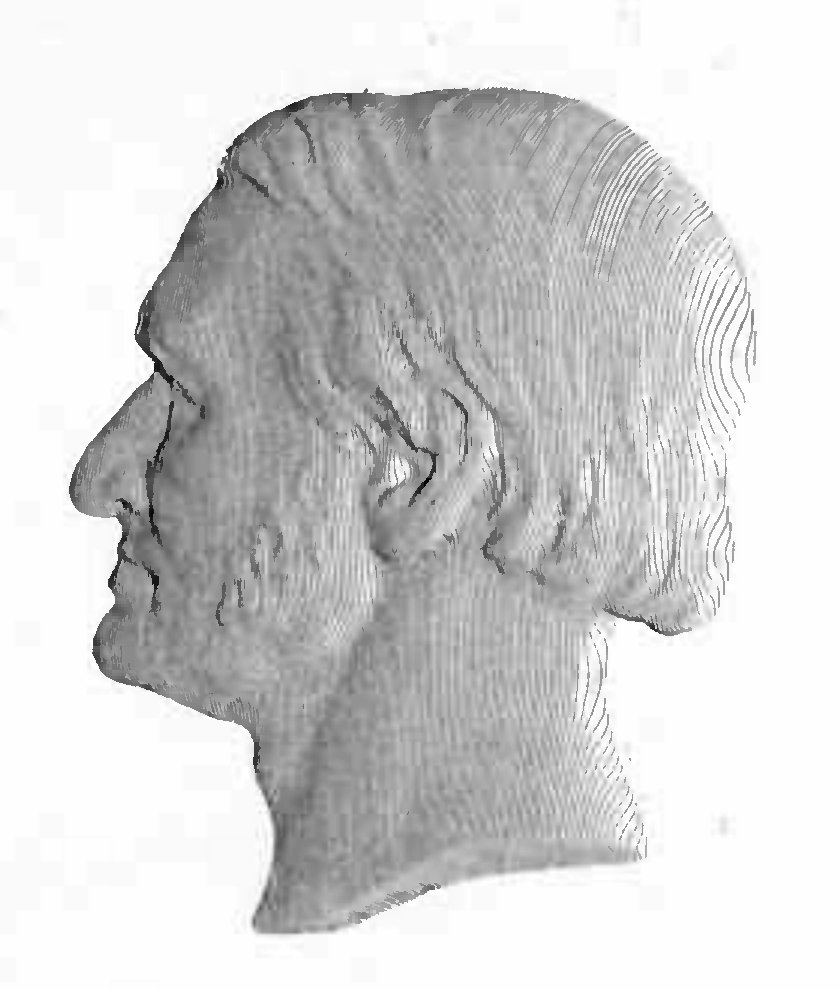
\includegraphics[width=1.6in]{assets/title_profile_contrast.png}\par
\vspace{.3in}{\large ZWEITER ABDRUCK\par}
\vspace{.2in}HERAUSGEGEBEN\par
\smallskip{\small VON DER\par}
\medskip{\small KÖNIGLICHEN GESELLSCHAFT DER WISSENSCHAFTEN\par}
\smallskip{\small ZU\par}
\medskip{\large GÖTTINGEN\par}
\smallskip1876.
\end{center}
\clearpage
\thispagestyle{empty}\SourceLeaf{11}
\pdfbookmark[0]{Ein neuer Beweis eines arithmetischen Satzes}{paper-one-title}
\begin{center}
\vspace*{.8in}
{\Large EIN NEUER BEWEIS\par}
\bigskip{\large EINES ARITHMETISCHEN SATZES\par}
\vspace{.6in}VON\par
\bigskip{\large CARL FRIEDRICH GAUSS\par}
\vspace{.3in}{\small DER KÖNIGLICHEN GESELLSCHAFT DER WISSENSCHAFTEN VORGELEGT AM 15. JANUAR 1808.\par}
\vspace{.65in}\rule{.85\linewidth}{.3pt}\par
\smallskip{\small Commentationes societatis regiae scientiarum Gottingensis. Vol. \textsc{xvi}.\par}
{\small Gottingae \textsc{mdcccviii}.\par}
\smallskip\rule{.85\linewidth}{.3pt}
\end{center}
\clearpage

\mainmatter
\SourceLeaf{13}
\begin{center}\Large EIN NEUER BEWEIS\end{center}

\begin{center}\large EINES ARITHMETISCHEN SATZES.\end{center}

\BookRule{35mm}

\Article{1}

Fragen der höheren Arithmetik zeigen sehr häufig eine eigentümliche Erscheinung, die in der Analysis viel seltener vorkommt und ihren Reiz erheblich steigert. Bei analytischen Untersuchungen können wir meist erst dann zu neuen Wahrheiten gelangen, wenn wir die Prinzipien, auf denen sie beruhen und die uns gleichsam den Weg zu ihnen öffnen müssen, zuvor gründlich beherrschen. In der Arithmetik dagegen treten sehr häufig durch Induktion und eine Art unerwarteten Glücks neue Wahrheiten von größter Eleganz hervor, deren Beweise so tief verborgen und in so große Dunkelheit gehüllt sind, dass sie sich allen Versuchen entziehen und selbst den scharfsinnigsten Untersuchungen den Zugang verwehren. Außerdem besteht zwischen arithmetischen Wahrheiten, die auf den ersten Blick völlig verschiedenartig erscheinen, ein so großer und wunderbarer Zusammenhang, dass wir nicht selten, während wir ganz anderes suchen, schließlich auf das Glücklichste zu dem so sehr ersehnten und zuvor in langen Überlegungen vergeblich gesuchten Beweis gelangen, und zwar auf einem ganz anderen Weg als dem erwarteten. Meist sind solche Wahrheiten aber von der Art, dass man auf mehreren sehr verschiedenen Wegen zu ihnen gelangen kann, und nicht immer sind die Wege, die sich zuerst anbieten, die kürzesten. Es muss daher gewiss hoch geschätzt werden, wenn es nach langer vergeblicher Untersuchung einer solchen Wahrheit, die dann zwar bewiesen wurde, aber auf ziemlich verborgenen Umwegen, schließlich gelingt, den einfachsten und eigentlichen Weg zu entdecken.

\Article{2}

Unter den im vorigen Artikel besprochenen Fragen nimmt der Satz einen hervorragenden Platz ein, der fast die gesamte Theorie der quadratischen Reste enthält und in den \emph{Untersuchungen über höhere Arithmetik} (Abschnitt IV) mit dem Namen \emph{Fundamentalsatz} ausgezeichnet \SourceLeaf{14}ist. Als \emph{erster} Entdecker dieses höchst eleganten Satzes ist ohne Zweifel der berühmte \textsc{Legendre} anzusehen, nachdem die großen Geometer \textsc{Euler} und \textsc{Lagrange} schon lange zuvor mehrere seiner besonderen Fälle durch Induktion entdeckt hatten. Ich halte mich hier nicht damit auf, die Beweisversuche dieser Männer aufzuzählen; wer möchte, möge das eben erwähnte Werk nachlesen. Zur Bestätigung des im vorigen Artikel Gesagten sei mir nur gestattet hinzuzufügen, was meine eigenen Versuche betrifft. Ich war im Jahr 1795 selbstständig auf den Satz gestoßen, als ich von allem, was in der höheren Arithmetik schon ausgearbeitet worden war, noch gar nichts wusste und von allen Hilfsmitteln der Literatur völlig abgeschnitten war. Doch ein ganzes Jahr lang quälte er mich und entzog sich meinen angestrengtesten Bemühungen, bis ich schließlich den im vierten Abschnitt jenes Werkes gegebenen Beweis fand. Später boten sich mir drei weitere an, die auf ganz verschiedenen Prinzipien beruhen; einen davon habe ich im fünften Abschnitt gegeben, die übrigen, die ihm an Eleganz nicht nachstehen, werde ich bei anderer Gelegenheit veröffentlichen. Doch alle diese Beweise scheinen zwar hinsichtlich ihrer Strenge nichts zu wünschen übrigzulassen, sind aber aus zu verschiedenartigen Prinzipien hergeleitet, vielleicht mit Ausnahme des ersten, der jedoch mit recht mühsamen Überlegungen vorgeht und durch ziemlich weitläufige Rechnungen belastet ist. Ich zögere daher nicht auszusprechen, dass bisher ein \emph{eigentlicher} Beweis gefehlt hat. Nun mögen die Sachkundigen beurteilen, ob der Beweis, den ich vor Kurzem entdeckt habe und den die folgenden Seiten enthalten, diesen Namen verdient.

\Article{3}

\textsc{Satz.} \emph{Es sei $p$ eine positive Primzahl; $k$ eine beliebige, durch $p$ nicht} \emph{teilbare ganze Zahl; es seien}

\[
\begin{aligned}
A &\quad \text{\emph{Gesamtheit der Zahlen}}\quad 1,\ 2,\ 3\ \dotsfour\ \tfrac12(p-1)\\
B &\quad \text{\emph{Gesamtheit dieser Zahlen}}\quad \tfrac12(p+1),\ \tfrac12(p+3),\ \tfrac12(p+5)\ \dotsfour\ p-1
\end{aligned}
\]

\emph{Man bilde die Produkte aus $k$ und den einzelnen Zahlen in $A$ und nehme ihre kleinsten positiven Reste modulo $p$, die offenbar alle verschieden sind und teils zu $A$, teils zu} \emph{$B$ gehören. Gehören nun zu $B$ insgesamt $\mu$ Reste, so ist $k$ ein quadratischer Rest oder Nichtrest von $p$, je nachdem $\mu$ gerade oder ungerade ist.}

\emph{Beweis.} Die zu $A$ gehörenden Reste seien $a,\ a'\ a''\ \dotsfour$, die übrigen, zu $B$ gehörenden $b,b',b''\dotsfour$. Offenbar sind die Ergänzungen der letzteren, $p-b,p-b',p-b''\dotsfour$, sämtlich von den Zahlen $a,\ a',\ a''\ \dotsfour$ verschieden, füllen aber mit diesen zusammen die Gesamtheit\SourceLeaf{15} $A$ aus. Wir haben also

\[
\begin{aligned}
1\pdot2\pdot3\ \dotsfour\ \tfrac12(p-1)=aa' a''\ \dotsfour\ (p-b)(p-b')(p-b'')\ \dotsfour
\end{aligned}
\]

Das letztere Produkt wird aber offenbar

\[
\begin{aligned}
&\equiv(-1)^\mu aa' a''\ \dotsfour\ bb' b''\ \dotsfour\ \equiv(-1)^\mu k\pdot2k\pdot3k\ \dotsfour\ \tfrac12(p-1)k\\
&\equiv(-1)^\mu k^{\frac12(p-1)}\,1\pdot2\pdot3\ \dotsfour\ \tfrac12(p-1) (\mathrm{mod.}p)
\end{aligned}
\]

\Needspace{7\baselineskip}Daher ist

\[
\begin{aligned}
1\equiv(-1)^\mu k^{\frac12(p-1)}
\end{aligned}
\]

oder $k^{\frac12(p-1)}\equiv\pm1$, je nachdem $\mu$ gerade oder ungerade ist; daraus folgt unser Satz unmittelbar.

\Article{4}

Durch die Einführung einiger geeigneter Bezeichnungen können wir die folgenden Überlegungen erheblich verkürzen. Das Zeichen $(k,p)$ soll uns daher die Anzahl derjenigen Produkte unter

\[
\begin{aligned}
k,\ 2k,\ 3k\ \dotsfour\ \tfrac12(p-1)k,
\end{aligned}
\]

bezeichnen, deren kleinste positive Reste modulo $p$ dessen Hälfte übersteigen. Ist ferner $x$ eine beliebige nicht ganze Größe, so bezeichnen wir mit dem Zeichen $[x]$ die unmittelbar unter $x$ liegende ganze Zahl, sodass $x-[x]$ stets eine positive Größe zwischen den Grenzen $0$ und $1$ ist. Die folgenden Beziehungen ergeben sich nun mit geringer Mühe:

I. $[x]+[-x]=-1.$

II. $[x]+h=[x+h]$, wenn $h$ eine ganze Zahl ist.

III. $[x]+[h-x]=h-1.$

IV. Ist $x-[x]$ ein Bruch kleiner als $\tfrac12$, so ist $[2x]-2[x]=0$; ist aber $x-[x]$ größer als $\tfrac12$, so ist $[2x]-2[x]=1.$

V. Liegt also der kleinste positive Rest der ganzen Zahl $h$ modulo $p$ unter $\tfrac12p$, so ist $\gbr{\frac{2h}{p}}-2\gbr{\frac{h}{p}}=0$; liegt jener Rest aber über $\tfrac12p$, so ist \mbox{$\gbr{\frac{2h}{p}}-2\gbr{\frac{h}{p}}=1.$}

\SourceLeaf{16}
VI. Daraus folgt sogleich $(k,p)=$

\[
\begin{aligned}
&\gbr{\frac{2k}{p}}+\gbr{\frac{4k}{p}}+\gbr{\frac{6k}{p}}\dotsfour+\gbr{\frac{(p-1)k}{p}}\\
&-2\gbr{\frac{k}{p}}-2\gbr{\frac{2k}{p}}-2\gbr{\frac{3k}{p}}\dotsfour-2\gbr{\frac{\frac12(p-1)k}{p}}.
\end{aligned}
\]

VII. Aus VI und I ergibt sich ohne Mühe

\[
\begin{aligned}
(k,p)+(-k,p)=\tfrac12(p-1)
\end{aligned}
\]

Daraus folgt, dass $-k$ dieselbe oder die entgegengesetzte Beziehung zu $p$ hat (insofern es dessen quadratischer Rest oder Nichtrest ist) wie $+k$, je nachdem $p$ die Form $4n+1$ oder die Form $4n+3$ hat. Im ersten Fall ist $-1$ offenbar ein Rest, im zweiten ein Nichtrest von $p$.

\Needspace{10\baselineskip}VIII. Die in VI gegebene Formel werden wir folgendermaßen umformen. Nach III ist

\[
\begin{aligned}
\gbr{\frac{(p-1)k}{p}}&=k-1-\gbr{\frac{k}{p}},\\
\gbr{\frac{(p-3)k}{p}}&=k-1-\gbr{\frac{3k}{p}},\\
\gbr{\frac{(p-5)k}{p}}&=k-1-\gbr{\frac{5k}{p}}\dotsfour
\end{aligned}
\]

Wenden wir diese Ersetzungen auf die letzten $\frac{p\mp1}{4}$ Glieder der oberen Reihe in jenem Ausdruck an, so erhalten wir

\Needspace{8\baselineskip}\emph{erstens}, wenn $p$ die Form $4n+1$ hat,

\[
\begin{aligned}
(k,p)&=\tfrac14(k-1)(p-1)\\
& -2\left\{\gbr{\frac{k}{p}}+\gbr{\frac{3k}{p}}+\gbr{\frac{5k}{p}}\dotsfour+\gbr{\frac{\frac12(p-3)k}{p}}\right\}\\
&\qquad-\left\{\gbr{\frac{k}{p}}+\gbr{\frac{2k}{p}}+\gbr{\frac{3k}{p}}\dotsfour+\gbr{\frac{\frac12(p-1)k}{p}}\right\}
\end{aligned}
\]

\Needspace{8\baselineskip}\emph{zweitens}, wenn $p$ die Form $4n+3$ hat,

\[
\begin{aligned}
(k,p)&=\tfrac14(k-1)(p+1)\\
& -2\left\{\gbr{\frac{k}{p}}+\gbr{\frac{3k}{p}}+\gbr{\frac{5k}{p}}\dotsfour+\gbr{\frac{\frac12(p-1)k}{p}}\right\}\\
&\qquad-\left\{\gbr{\frac{k}{p}}+\gbr{\frac{2k}{p}}+\gbr{\frac{3k}{p}}\dotsfour+\gbr{\frac{\frac12(p-1)k}{p}}\right\}
\end{aligned}
\]

IX. Für den besonderen Fall $k=+2$ folgt aus den eben gegebenen Formeln $(2,p)=\tfrac14(p\mp1)$, wobei das obere oder untere Zeichen zu nehmen ist, je nachdem $p$ die Form $4n+1$ oder $4n+3$ hat. Somit ist $(2,p)$ gerade, also $2Rp$, wenn $p$ die Form $8n+1$ oder $8n+7$ hat; dagegen ist $(2,p)$ ungerade und $2Np$, wenn $p$ die Form $8n+3$ oder $8n+5$ hat.

\SourceLeaf{17}
\Needspace{14\baselineskip}\Article{5}

\textsc{Satz.} \emph{Es sei $x$ eine positive nicht ganze Größe, unter deren Vielfachen $x$, $2x$,} \emph{$3x\dotsfour$ bis $nx$ keines eine ganze Zahl ist; man setze $[nx]=h$, woraus leicht folgt,} \emph{dass auch unter den Vielfachen der reziproken Größe $\frac1x$, $\frac2x$, $\frac3x\dotsfive$ bis $\frac hx$ keine ganze Zahl} \emph{vorkommt. Dann behaupte ich, es sei}

\[
\begin{aligned}
\left.\begin{aligned}
&[x]+[2x]+[3x]\dotstwo+[nx]\\
&+\gbr{\frac1x}+\gbr{\frac2x}+\gbr{\frac3x}\dotsfour+\gbr{\frac hx}
\end{aligned}\right\}=nh.
\end{aligned}
\]

\emph{Beweis.} In der Reihe $[x]+[2x]+[3x]\dotsfour+[nx]$, die wir $=\Omega$ setzen, sind die ersten Glieder bis einschließlich des Gliedes an der Stelle $\gbr{\frac1x}$ offenbar alle $=0$; die folgenden bis zum Glied an der Stelle $\gbr{\frac2x}$ sämtlich $=1$; die folgenden bis zum Glied an der Stelle $\gbr{\frac3x}$ sämtlich $=2$, und so weiter. Daher ist

\[
\begin{aligned}
\left.\begin{aligned}
\Omega={}&0\times\gbr{\frac1x}\\
&+1\times\left\{\gbr{\frac2x}-\gbr{\frac1x}\right\}\\
&+2\times\left\{\gbr{\frac3x}-\gbr{\frac2x}\right\}\\
&+3\times\left\{\gbr{\frac4x}-\gbr{\frac3x}\right\}\\
&\hspace{12mm}\text{usw.}\\
&+(h-1)\left\{\gbr{\frac hx}-\gbr{\frac{h-1}{x}}\right\}\\
&+h\left\{n-\gbr{\frac hx}\right\}
\end{aligned}\right\}=hn-\gbr{\frac1x}-\gbr{\frac2x}-\gbr{\frac3x}\dotsfour-\gbr{\frac hx}
\end{aligned}
\]

Q. E. D.

\Needspace{12\baselineskip}\Article{6}

\textsc{Satz.} \emph{Bezeichnen $k,p$ beliebige positive ungerade, zueinander teilerfremde Zahlen, so ist}

\[
\begin{aligned}
\left.\begin{aligned}
&\gbr{\frac kp}+\gbr{\frac{2k}{p}}+\gbr{\frac{3k}{p}}\dotsfour+\gbr{\frac{\frac12(p-1)k}{p}}\\
&+\gbr{\frac pk}+\gbr{\frac{2p}{k}}+\gbr{\frac{3p}{k}}\dotsfour+\gbr{\frac{\frac12(k-1)p}{k}}
\end{aligned}\right\}=\tfrac14(k-1)(p-1).
\end{aligned}
\]

\emph{Beweis.} Nehmen wir, was erlaubt ist, $k<p$ an, so ist $\frac{\frac12(p-1)k}{p}$ kleiner als $\frac12 k$, aber größer als $\frac12(k-1)$, also $\gbr{\frac{\frac12(p-1)k}{p}}=\frac12(k-1)$. Daraus ergibt sich offenbar der vorliegende Satz unmittelbar aus dem vorhergehenden, wenn man dort $\frac kp=x$, $\frac12(p-1)=n$, also $\frac12(k-1)=h$ setzt.

\SourceLeaf{18}
\Needspace{8\baselineskip}Übrigens lässt sich auf ähnliche Weise beweisen, dass, wenn $k$ eine zu $p$ teilerfremde \emph{gerade} Zahl ist, gilt:

\[
\begin{aligned}
\left.\begin{aligned}
&\gbr{\frac kp}+\gbr{\frac{2k}{p}}+\gbr{\frac{3k}{p}}\dotsfour+\gbr{\frac{\frac12(p-1)k}{p}}\\
&+\gbr{\frac pk}+\gbr{\frac{2p}{k}}+\gbr{\frac{3p}{k}}\dotsfour+\gbr{\frac{\frac12 kp}{k}}
\end{aligned}\right\}=\tfrac14 k(p-1)
\end{aligned}
\]

Doch halten wir uns bei diesem für unser Vorhaben nicht notwendigen Satz nicht auf.

\clearpage\Article{7}

Aus der Verbindung des vorhergehenden Satzes mit der Aussage VIII des Artikels 4 folgt nun unmittelbar der Fundamentalsatz. Bezeichnen nämlich $k,p$ beliebige verschiedene positive Primzahlen, und setzen wir

\[
\begin{aligned}
(k,p)+\gbr{\frac kp}+\gbr{\frac{2k}{p}}+\gbr{\frac{3k}{p}}\dotsfour+\gbr{\frac{\frac12(p-1)k}{p}}&=L\\
(p,k)+\gbr{\frac pk}+\gbr{\frac{2p}{k}}+\gbr{\frac{3p}{k}}\dotsfour+\gbr{\frac{\frac12(k-1)p}{k}}&=M
\end{aligned}
\]

so ist nach VIII des Artikels 4 klar, dass $L$ und $M$ stets gerade Zahlen sind. Nach dem Satz des Artikels 6 ist aber

\[
\begin{aligned}
L+M=(k,p)+(p,k)+\tfrac14(k-1)(p-1)
\end{aligned}
\]

Wann immer also $\frac14(k-1)(p-1)$ gerade ist, was geschieht, wenn für beide $k,p$ oder wenigstens für eine von ihnen die Form $4n+1$ vorliegt, müssen $(k,p)$ und $(p,k)$ notwendig entweder beide gerade oder beide ungerade sein. Ist hingegen $\frac14(k-1)(p-1)$ ungerade, was geschieht, wenn beide $k,p$ die Form $4n+3$ haben, so muss notwendig eine der Zahlen $(k,p)$, $(p,k)$ gerade, die andere ungerade sein. Im ersten Fall sind daher die Beziehung von $k$ zu $p$ und die Beziehung von $p$ zu $k$ (insofern eine der beiden ein Rest oder Nichtrest der anderen ist) gleich, im zweiten entgegengesetzt.

Q. E. D.

\BookRule{35mm}


\clearpage
\def\BookRunningTitle{Summation einiger besonderer Reihen}
\renewcommand{\Article}[1]{\par\medskip\Needspace{4\baselineskip}\pdfbookmark[1]{Art. #1}{paper-two-art-#1}\centerline{\textbf{#1.}}\nobreak\smallskip}
\clearpage\thispagestyle{empty}\SourceLeaf{19}
\pdfbookmark[0]{Summation einiger besonderer Reihen}{paper-two-title}
\begin{center}
\vspace*{.6in}{\large SUMMATION\par}
\bigskip{\Large EINIGER BESONDERER\par}
\bigskip{\large REIHEN\par}
\vspace{.65in}VON\par
\bigskip{\large CARL FRIEDRICH GAUSS\par}
\vspace{.3in}{\small DER GESELLSCHAFT VORGELEGT AM XXIV. AUGUST MDCCCVIII.\par}
\vspace{.6in}\rule{.85\linewidth}{.3pt}\par
\smallskip{\small Commentationes societatis regiae scientiarum Gottingensis recentiores. Vol. \textsc{i}.\par}
{\small Gottingae \textsc{mdcccxi}.\par}
\smallskip\rule{.85\linewidth}{.3pt}
\end{center}

\clearpage
\SourceLeaf{21}
\begin{center}\Large SUMMATION\end{center}

\begin{center}\large EINIGER BESONDERER REIHEN.\end{center}

\BookRule{22mm}

\Article{1}

Unter den bedeutenderen Wahrheiten, zu denen die Theorie der Kreisteilung den Zugang eröffnet hat, nimmt die in den Disquiss. Arithmet., Art. 356, angegebene Summation einen hervorragenden Platz ein. Das liegt sowohl an ihrer besonderen Eleganz und erstaunlichen Fruchtbarkeit, die eine andere Untersuchung später ausführlicher darzustellen Gelegenheit geben wird, als auch an den ungewöhnlichen Schwierigkeiten ihres strengen und vollständigen Beweises.\quad Diese Schwierigkeiten hätte man umso weniger erwarten sollen, als sie weniger den Satz selbst als vielmehr eine gewisse Einschränkung des Satzes betreffen: Lässt man diese außer Betracht, so steht sofort ein Beweis zur Verfügung, der sich sehr leicht aus der in jenem Werk entwickelten Theorie ergibt.\quad Der Satz wurde dort in folgender Form angegeben.\quad Es sei $n$ eine Primzahl; alle quadratischen Reste von $n$ zwischen den Grenzen $1$ und $n-1$ einschließlich seien unbestimmt durch $a$ bezeichnet und alle Nichtreste zwischen denselben Grenzen durch $b$, schließlich bezeichne $\omega$ den Bogen $\frac{360^{0}}{n}$ und $k$ eine beliebige feste ganze Zahl, die nicht durch $n$ teilbar ist. Dann gilt

I.\quad für einen Wert von $n$ von der Form $4m+1$:

\[
\begin{aligned}
\Sigma\cos ak\omega&=-\tfrac12\pm\tfrac12\surd n\\
\Sigma\cos bk\omega&=-\tfrac12\mp\tfrac12\surd n,\ \text{und somit}\\
\Sigma\cos ak\omega-\Sigma\cos bk\omega&=\pm\surd n\\
\Sigma\sin ak\omega&=0\\
\Sigma\sin bk\omega&=0
\end{aligned}
\]

\SourceLeaf{22}
II.\quad für einen Wert von $n$ von der Form $4m+3$:

\[
\begin{aligned}
\Sigma\cos ak\omega&=-\tfrac12\\
\Sigma\cos bk\omega&=-\tfrac12\\
\Sigma\sin ak\omega&=\pm\tfrac12\surd n\\
\Sigma\sin bk\omega&=\mp\tfrac12\surd n\\
\Sigma\sin ak\omega-\Sigma\sin bk\omega&=\pm\surd n
\end{aligned}
\]

Diese Summationen sind an der angeführten Stelle mit voller Strenge bewiesen worden. Hier bleibt nur die Schwierigkeit, das \emph{Vorzeichen} zu bestimmen, das vor den Wurzelausdruck zu setzen ist.\quad Ohne Mühe lässt sich zwar zeigen, dass dieses Vorzeichen insofern von der Zahl $k$ abhängt, als für alle Werte von $k$, die quadratische Reste von $n$ sind, stets \emph{dasselbe} Vorzeichen gelten muss und für alle Werte von $k$, die quadratische Nichtreste von $n$ sind, das entgegengesetzte.\quad Damit kommt es nur auf den Wert $k=1$ an: Sobald das für diesen Wert geltende Vorzeichen bekannt ist, stehen auch die Vorzeichen für alle übrigen Werte von $k$ sofort zur Verfügung.\quad Doch gerade bei dieser Frage, die auf den ersten Blick zu den leichteren zu gehören scheint, stoßen wir auf unerwartete Schwierigkeiten, und die Methode, unter deren Führung wir bisher ohne Hindernisse vorangekommen waren, verweigert jede weitere Hilfe.

\Article{2}

Bevor wir weitergehen, wird es nützlich sein, einige Beispiele unserer Summation zahlenmäßig durchzurechnen; zuvor sollen jedoch einige allgemeine Beobachtungen stehen.

I.\quad Im Fall, dass $n$ eine Primzahl von der Form $4m+1$ ist, seien alle quadratischen Reste von $n$ zwischen $1$ und $\frac12(n-1)$ einschließlich unbestimmt durch $a'$ und alle Nichtreste zwischen denselben Grenzen durch $b'$ dargestellt. Bekanntlich sind dann alle $n-a'$ unter den $a$ und alle $n-b'$ unter den $b$ enthalten. Da alle $a'$, $b'$, $n-a'$, $n-b'$ zusammen offenbar die gesamte Menge der Zahlen $1$, $2$, $3\dotsfour$ $n-1$ ausfüllen, umfassen alle $a'$ zusammen mit allen $n-a'$ sämtliche $a$; ebenso umfassen alle $b'$ zusammen mit allen $n-b'$ sämtliche $b$.\quad Daher ist

\SourceLeaf{23}
\[
\begin{aligned}
\Sigma\cos ak\omega&=\Sigma\cos a'k\omega+\Sigma\cos(n-a')k\omega\\
\Sigma\cos bk\omega&=\Sigma\cos b'k\omega+\Sigma\cos(n-b')k\omega\\
\Sigma\sin ak\omega&=\Sigma\sin a'k\omega+\Sigma\sin(n-a')k\omega\\
\Sigma\sin bk\omega&=\Sigma\sin b'k\omega+\Sigma\sin(n-b')k\omega
\end{aligned}
\]

Da nun $\cos(n-a')k\omega=\cos a'k\omega$, $\cos(n-b')k\omega=\cos b'k\omega$, $\sin(n-a')k\omega=-\sin a'k\omega$, $\sin(n-b')k\omega=-\sin b'k\omega$ gilt, ergibt sich unmittelbar

\[
\begin{aligned}
\Sigma\sin ak\omega&=\Sigma\sin a'k\omega-\Sigma\sin a'k\omega=0\\
\Sigma\sin bk\omega&=\Sigma\sin b'k\omega-\Sigma\sin b'k\omega=0
\end{aligned}
\]

Die Summation der Kosinus nimmt dagegen die Form

\[
\begin{aligned}
\Sigma\cos ak\omega&=2\Sigma\cos a'k\omega\\
\Sigma\cos bk\omega&=2\Sigma\cos b'k\omega
\end{aligned}
\]

an, sodass gelten muss:

\[
\begin{aligned}
1+4\Sigma\cos a'k\omega&=\pm\surd n\\
1+4\Sigma\cos b'k\omega&=\mp\surd n\\
2\Sigma\cos a'k\omega-2\Sigma\cos b'k\omega&=\pm\surd n
\end{aligned}
\]

II.\quad Im Fall, dass $n$ von der Form $4m+3$ ist, ist die Ergänzung jedes Restes $a$ zu $n$ ein Nichtrest und die Ergänzung jedes $b$ ein Rest. Somit stimmen sämtliche $n-a$ mit sämtlichen $b$ und sämtliche $n-b$ mit sämtlichen $a$ überein. Daraus folgt

\[
\begin{aligned}
\Sigma\cos ak\omega=\Sigma\cos(n-b)k\omega=\Sigma\cos bk\omega
\end{aligned}
\]

Da also sämtliche $a$ und $b$ zusammen alle Zahlen $1$, $2$, $3\dotsfour n-1$ ausfüllen und somit $\Sigma\cos ak\omega+\Sigma\cos bk\omega=\cos k\omega+\cos2k\omega+\cos3k\omega+\text{usw.}$ $+\cos(n-1)k\omega=-1$ gilt, ergeben sich die Summationen

\[
\begin{aligned}
\Sigma\cos ak\omega&=-\tfrac12\\
\Sigma\cos bk\omega&=-\tfrac12
\end{aligned}
\]

unmittelbar.\quad Ebenso ist

\[
\begin{aligned}
\Sigma\sin ak\omega=\Sigma\sin(n-b)k\omega=-\Sigma\sin bk\omega
\end{aligned}
\]

\SourceLeaf{24}
woraus ersichtlich ist, wie von den beiden Summationen

\[
\begin{aligned}
2\Sigma\sin ak\omega&=\pm\surd n\\
2\Sigma\sin bk\omega&=\mp\surd n
\end{aligned}
\]

die eine von der anderen abhängt.

\Article{3}

Hier folgen nun die Zahlenrechnungen für einige Beispiele:

I.\quad Für $n=5$ gibt es einen Wert von $a'$, nämlich $a'=1$, und einen Wert von $b'$, nämlich $b'=2$. Es ist

\[
\begin{aligned}
\cos\omega=+0{,}3090169944\qquad\cos2\omega=-0{,}8090169944
\end{aligned}
\]

und somit $1+4\cos\omega=+\surd5$,\quad $1+4\cos2\omega=-\surd5$.

II.\quad Für $n=13$ gibt es drei Werte von $a'$, nämlich $1$, $3$, $4$, und ebenso viele Werte von $b'$, nämlich $2$, $5$, $6$. Daraus berechnen wir

{\small\setlength{\arraycolsep}{2.5pt}\renewcommand{\arraystretch}{1.15}
\[
\begin{array}{rclcrcl}
\cos\omega&=&+0{,}8854560257&\qquad&\cos2\omega&=&+0{,}5680647467\\
\cos3\omega&=&+0{,}1205366803&\qquad&\cos5\omega&=&-0{,}7485107482\\
\cos4\omega&=&-0{,}3546048870&\qquad&\cos6\omega&=&-0{,}9709418174\\\cline{1-3}\cline{5-7}
\text{Summe}&=&+0{,}6513878190&\qquad&\text{Summe}&=&-1{,}1513878189
\end{array}
\]
}

Daher $1+4\Sigma\cos a'\omega=+\surd13$,\quad $1+4\Sigma\cos b'\omega=-\surd13$.

\Needspace{13\baselineskip}III.\quad Für $n=17$ haben wir vier Werte von $a'$, nämlich $1$, $2$, $4$, $8$, und ebenso viele Werte von $b'$, nämlich $3$, $5$, $6$, $7$.\quad Daraus berechnen sich die Kosinus:

{\small\setlength{\arraycolsep}{2.5pt}\renewcommand{\arraystretch}{1.15}
\[
\begin{array}{rclcrcl}
\cos\omega&=&+0{,}9324722294&\qquad&\cos3\omega&=&+0{,}4457383558\\
\cos2\omega&=&+0{,}7390089172&\qquad&\cos5\omega&=&-0{,}2736629901\\
\cos4\omega&=&+0{,}0922683595&\qquad&\cos6\omega&=&-0{,}6026346364\\
\cos8\omega&=&-0{,}9829730997&\qquad&\cos7\omega&=&-0{,}8502171357\\\cline{1-3}\cline{5-7}
\text{Summe}&=&+0{,}7807764064&\qquad&\text{Summe}&=&-1{,}2807764065
\end{array}
\]
}

Daher $1+4\Sigma\cos a'\omega=+\surd17$,\quad $1+4\Sigma\cos b'\omega=-\surd17$.

\SourceLeaf{25}
IV.\quad Für $n=3$ gibt es nur einen Wert von $a$, nämlich $a=1$, dem

\[
\begin{aligned}
\sin\omega=+0{,}8660254038
\end{aligned}
\]

entspricht. Daher $2\sin\omega=+\surd3$.

V.\quad Für $n=7$ gibt es drei Werte von $a$, nämlich $1$, $2$, $4$. Daraus ergeben sich die Sinus:

{\small\setlength{\arraycolsep}{2.5pt}\renewcommand{\arraystretch}{1.15}
\[
\begin{array}{rcll}
\sin\omega&=&+0{,}7818314825&\\
\sin2\omega&=&+0{,}9749279122&\\
\sin4\omega&=&-0{,}4338837391&\\\cline{1-3}
\text{Summe}&=&+1{,}3228756556,&\text{und somit }2\Sigma\sin a\omega=+\surd7.
\end{array}
\]
}

VI.\quad Für $n=11$ sind die Werte von $a$ gleich $1$, $3$, $4$, $5$, $9$. Ihnen entsprechen die Sinus:

{\small\setlength{\arraycolsep}{2.5pt}\renewcommand{\arraystretch}{1.15}
\[
\begin{array}{rcll}
\sin\omega&=&+0{,}5406408175&\\
\sin3\omega&=&+0{,}9898214419&\\
\sin4\omega&=&+0{,}7557495744&\\
\sin5\omega&=&+0{,}2817325568&\\
\sin9\omega&=&-0{,}9096319954&\\\cline{1-3}
\text{Summe}&=&+1{,}6583123952,&\text{und daher }2\Sigma\sin a\omega=+\surd11.
\end{array}
\]
}

\Needspace{19\baselineskip}VII.\quad Für $n=19$ sind die Werte von $a$ gleich $1$, $4$, $5$, $6$, $7$, $9$, $11$, $16$, $17$. Ihnen entsprechen die Sinus:

{\small\setlength{\arraycolsep}{2.5pt}\renewcommand{\arraystretch}{1.15}
\[
\begin{array}{rcll}
\sin\omega&=&+0{,}3246994692&\\
\sin4\omega&=&+0{,}9694002659&\\
\sin5\omega&=&+0{,}9965844930&\\
\sin6\omega&=&+0{,}9157733267&\\
\sin7\omega&=&+0{,}7357239107&\\
\sin9\omega&=&+0{,}1645945903&\\
\sin11\omega&=&-0{,}4759473930&\\
\sin16\omega&=&-0{,}8371664783&\\
\sin17\omega&=&-0{,}6142127127&\\\cline{1-3}
\text{Summe}&=&+2{,}1794494718,&\text{und somit }2\Sigma\sin a\omega=+\surd19.
\end{array}
\]
}

\SourceLeaf{26}
\Article{4}

In allen diesen Beispielen erhält der Wurzelausdruck das positive Vorzeichen. Dasselbe bestätigt sich leicht auch für die größeren Werte $n=23$, $n=29$ usw.; daraus ergibt sich bereits eine hohe Wahrscheinlichkeit, dass dies ebenso allgemein gilt.\quad Ein Beweis dieser Erscheinung lässt sich jedoch nicht aus den an der angeführten Stelle dargelegten Grundsätzen gewinnen; mit vollem Recht ist sie als Gegenstand einer tieferen Untersuchung anzusehen.\quad Diese Abhandlung soll daher einen strengen Beweis dieses höchst eleganten Satzes vorlegen, der zuvor mehrere Jahre lang auf verschiedene Weise vergeblich versucht worden war und schließlich durch ungewöhnliche und recht subtile Überlegungen gelang. Zugleich werden wir den Satz unter Wahrung, oder vielmehr Steigerung, seiner Eleganz zu weit größerer Allgemeinheit führen.\quad Als krönenden Abschluss werden wir schließlich den erstaunlichen und sehr engen Zusammenhang zwischen dieser Summation und einem anderen arithmetischen Satz von höchster Bedeutung zeigen.\quad Wir hoffen, dass diese Untersuchungen den Geometern an sich willkommen sein werden und dass auch die Methoden, durch die wir all dies erreichen konnten und die bei anderen Gelegenheiten ebenfalls nützlich sein können, ihrer Aufmerksamkeit würdig erscheinen werden.

\Article{5}

Unser Beweis geht aus der Betrachtung einer besonderen Art von Reihen hervor, deren Glieder von Ausdrücken wie

\[
\begin{aligned}
\frac{(1-x^m)\,(1-x^{m-1})\,(1-x^{m-2})\dotsfour(1-x^{m-\mu+1})}{(1-x)\,(1-xx)\,(1-x^3)\dotsfive(1-x^\mu)}
\end{aligned}
\]

abhängen. Der Kürze halber bezeichnen wir einen solchen Bruch mit $(m,\mu)$ und schicken zunächst einige allgemeine Beobachtungen über solche Funktionen voraus.

\Needspace{19\baselineskip}I.\quad Ist $m$ eine positive ganze Zahl kleiner als $\mu$, so verschwindet die Funktion $(m,\mu)$ offenbar, da der Zähler den Faktor $1-x^0$ enthält.\quad Für $m=\mu$ stimmen die Faktoren im Zähler in umgekehrter Reihenfolge mit denen im Nenner überein, woraus $(\mu,\mu)=1$ folgt. Für den Fall schließlich, dass $m$ eine positive ganze Zahl größer als $\mu$ ist, gelten die Formeln

\[
\begin{aligned}
(\mu+1,\mu)&=\frac{1-x^{\mu+1}}{1-x}=(\mu+1,1)\\
(\mu+2,\mu)&=\frac{(1-x^{\mu+2})\,(1-x^{\mu+1})}{(1-x)\qquad(1-xx)}=(\mu+2,2)\\
(\mu+3,\mu)&=\frac{(1-x^{\mu+3})(1-x^{\mu+2})(1-x^{\mu+1})}{(1-x)\qquad(1-xx)\qquad(1-x^3)}=(\mu+3,3)\ \text{usw.}
\end{aligned}
\]

\SourceLeaf{27}
oder allgemein

\[
\begin{aligned}
(m,\mu)=(m,m-\mu)
\end{aligned}
\]

II.\quad Ferner bestätigt sich leicht, dass allgemein

\[
\begin{aligned}
(m,\mu+1)=(m-1,\mu+1)+x^{m-\mu-1}(m-1,\mu)
\end{aligned}
\]

gilt. Da ebenso

\[
\begin{aligned}
(m-1,\mu+1)&=(m-2,\mu+1)+x^{m-\mu-2}(m-2,\mu)\\
(m-2,\mu+1)&=(m-3,\mu+1)+x^{m-\mu-3}(m-3,\mu)\\
(m-3,\mu+1)&=(m-4,\mu+1)+x^{m-\mu-4}(m-4,\mu),\ \text{usw.}
\end{aligned}
\]

ist und diese Reihe bis zu

\[
\begin{aligned}
(\mu+2,\mu+1)&=(\mu+1,\mu+1)+x(\mu+1,\mu)\\
&=(\mu,\mu)+x(\mu+1,\mu)
\end{aligned}
\]

fortgesetzt werden kann, sofern $m$ eine positive ganze Zahl größer als $\mu+1$ ist, ergibt sich

\[
\begin{aligned}
(m,\mu+1)&=(\mu,\mu)+x(\mu+1,\mu)+xx(\mu+2,\mu)\\
&\qquad+x^3(\mu+3,\mu)+\text{usw.}\\
&\qquad+x^{m-\mu-1}(m-1,\mu)
\end{aligned}
\]

\Needspace{16\baselineskip}Daraus ist ersichtlich: Ist für einen bestimmten Wert von $\mu$ jede Funktion $(m,\mu)$ bei positivem ganzzahligem $m$ ein Polynom, so muss auch jede Funktion $(m,\mu+1)$ ein Polynom sein.\quad Da diese Voraussetzung für $\mu=1$ zutrifft, gilt sie also auch für $\mu=2$ und damit auch für $\mu=3$ usw. Das heißt, allgemein ist für jeden positiven ganzzahligen Wert von $m$ die Funktion $(m,\mu)$ ein Polynom; gleichbedeutend damit ist das Produkt

\[
\begin{aligned}
(1-x^m)(1-x^{m-1})(1-x^{m-2})\dotsfour(1-x^{m-\mu+1})
\end{aligned}
\]

teilbar durch

\[
\begin{aligned}
(1-x)(1-x^2)(1-x^3)\dotsfour(1-x^\mu)
\end{aligned}
\]

\clearpage\Needspace{14\baselineskip}\Article{6}

Wir betrachten nun zwei Reihen, die beide zu unserem Ziel führen können.\quad Die erste Reihe ist

\SourceLeaf{28}
\[
\begin{aligned}
&1-\frac{1-x^m}{1-x}+\frac{(1-x^m)\,(1-x^{m-1})}{(1-x)\,(1-xx)}\\
&\qquad-\frac{(1-x^m)(1-x^{m-1})(1-x^{m-2})}{(1-x)\quad(1-xx)\quad(1-x^3)}+\text{usw.}
\end{aligned}
\]

oder

\[
\begin{aligned}
1-(m,1)+(m,2)-(m,3)+(m,4)-\text{usw.}
\end{aligned}
\]

die wir der Kürze halber mit $f(x,m)$ bezeichnen.\quad Zunächst ist unmittelbar ersichtlich, dass diese Reihe, sobald $m$ eine positive ganze Zahl ist, nach ihrem Glied an der Stelle $m+1$ (wobei $=\pm1$ gilt) \emph{abbricht} und dass ihre Summe in diesem Fall daher ein endliches Polynom in $x$ sein muss.\quad Ferner ergibt sich aus Art. 5, II, dass allgemein für jeden Wert von $m$

\[
\begin{aligned}
1&=1\\
-(m,1)&=-(m-1,1)-x^{m-1}\\
+(m,2)&=+(m-1,2)+x^{m-2}(m-1,1)\\
-(m,3)&=-(m-1,3)-x^{m-3}(m-1,2),\ \text{usw.}
\end{aligned}
\]

und somit

\[
\begin{aligned}
f(x,m)&=1-x^{m-1}-(1-x^{m-2})(m-1,1)\\
&\qquad+(1-x^{m-3})(m-1,2)\\
&\qquad-(1-x^{m-4})(m-1,3)+\text{usw.}
\end{aligned}
\]

gilt. Offenbar ist aber

\[
\begin{aligned}
(1-x^{m-2})(m-1,1)&=(1-x^{m-1})(m-2,1)\\
(1-x^{m-3})(m-1,2)&=(1-x^{m-1})(m-2,2)\\
(1-x^{m-4})(m-1,3)&=(1-x^{m-1})(m-2,3),\ \text{usw.}
\end{aligned}
\]

woraus wir die folgende Gleichung ableiten:

\[
\begin{aligned}
f(x,m)=(1-x^{m-1})f(x,m-2)\ .\ .\ .\ .\ .\ .\ .\ .\ [1]
\end{aligned}
\]

\clearpage\Needspace{11\baselineskip}\Article{7}

Da für $m=0$ die Gleichung $f(x,m)=1$ gilt, ergibt die soeben gefundene Formel

\[
\begin{aligned}
f(x,2)&=1-x\\
f(x,4)&=(1-x)(1-x^3)\\
f(x,6)&=(1-x)(1-x^3)(1-x^5)\\
f(x,8)&=(1-x)(1-x^3)(1-x^5)(1-x^7),\ \text{usw.}
\end{aligned}
\]

oder allgemein für jeden geraden Wert von $m$:

\[
\begin{aligned}
f(x,m)=(1-x)(1-x^3)(1-x^5)\dotsfour(1-x^{m-1})\ .\ .\ .\ [2].
\end{aligned}
\]

\SourceLeaf{29}
Da hingegen für $m=1$ die Gleichung $f(x,m)=0$ gilt, ist auch

\[
\begin{aligned}
f(x,3)&=0\\
f(x,5)&=0\\
f(x,7)&=0\ \text{usw.}
\end{aligned}
\]

oder allgemein für jeden ungeraden Wert von $m$:

\[
\begin{aligned}
f(x,m)=0
\end{aligned}
\]

Die letztere Summation hätte man im Übrigen schon daraus ableiten können, dass in der Reihe

\[
\begin{aligned}
1-(m,1)+(m,2)-(m,3)+\text{usw.}+(m,m-1)-(m,m)
\end{aligned}
\]

das letzte Glied das erste aufhebt, das vorletzte das zweite usw.

\Article{8}

Für unser Ziel genügt zwar der Fall, dass $m$ eine positive ungerade ganze Zahl ist. Wegen der Eigenart des Gegenstands lohnt es sich aber, auch über die Fälle, in denen $m$ gebrochen oder negativ ist, einiges hinzuzufügen.\quad Unsere Reihe bricht dann offenbar nicht mehr ab, sondern läuft ins Unendliche; außerdem sieht man leicht, dass sie divergent wird, sobald $x$ ein Wert kleiner als $1$ gegeben wird. Ihre Summation muss daher auf Werte von $x$ beschränkt werden, die größer als $1$ sind.

\Needspace{13\baselineskip}Nach Formel [1] in Art. 6 haben wir

\[
\begin{aligned}
f(x,-2)&=\frac{1}{1-\frac1x}\\[8pt]
f(x,-4)&=\frac{1}{1-\frac1x}\pdot\frac{1}{1-\frac1{x^3}}\\[8pt]
f(x,-6)&=\frac{1}{1-\frac1x}\pdot\frac{1}{1-\frac1{x^3}}\pdot\frac{1}{1-\frac1{x^5}},\ \text{usw.}
\end{aligned}
\]

sodass sich der Wert der Funktion $f(x,m)$ auch für einen negativen geraden ganzzahligen Wert von $m$ in endlichen Gliedern angeben lässt.\quad Für die übrigen Werte von $m$ werden wir die Funktion $f(x,m)$ dagegen auf folgende Weise in ein \emph{unendliches Produkt} umwandeln.

Wenn $m$ einem negativen \emph{unendlichen} Wert zustrebt, geht die Funktion $f(x,m)$ über in

\SourceLeaf{30}
\[
\begin{aligned}
&1+\frac1{x-1}+\frac1{x-1}\pdot\frac1{xx-1}\\
&\qquad+\frac1{x-1}\pdot\frac1{xx-1}\pdot\frac1{x^3-1}+\text{usw.}
\end{aligned}
\]

Diese Reihe ist also gleich dem unendlichen Produkt

\[
\begin{aligned}
\frac1{1-\frac1x}\pdot\frac1{1-\frac1{x^3}}\pdot\frac1{1-\frac1{x^5}}\pdot\frac1{1-\frac1{x^7}}\;\text{usw. bis ins Unendliche.}
\end{aligned}
\]

Da ferner allgemein

\[
\begin{aligned}
f(x,m)&=f(x,m-2\lambda)\pdot(1-x^{m-1})(1-x^{m-3})\\
&\qquad(1-x^{m-5})\dotstwo(1-x^{m-2\lambda+1})
\end{aligned}
\]

ist, gilt

\[
\begin{aligned}
f(x,m)&=f(x,-\infty)\pdot(1-x^{m-1})(1-x^{m-3})(1-x^{m-5})\\
&\qquad\text{usw. bis ins Unendliche.}\\
&=\frac{1-x^{m-1}}{1-x^{-1}}\pdot\frac{1-x^{m-3}}{1-x^{-3}}\pdot\frac{1-x^{m-5}}{1-x^{-5}}\pdot\frac{1-x^{m-7}}{1-x^{-7}}\\
&\qquad\text{usw. bis ins Unendliche.}
\end{aligned}
\]

Dessen Faktoren nähern sich im weiteren Verlauf offenbar immer mehr der Einheit.

Besondere Aufmerksamkeit verdient der Fall $m=-1$. Hier ist

\[
\begin{aligned}
f(x,-1)=1+x^{-1}+x^{-3}+x^{-6}+x^{-10}+\text{usw.}
\end{aligned}
\]

\Needspace{9\baselineskip}Diese Reihe ist also gleich dem unendlichen Produkt

\[
\begin{aligned}
\frac{1-x^{-2}}{1-x^{-1}}\pdot\frac{1-x^{-4}}{1-x^{-3}}\pdot\frac{1-x^{-6}}{1-x^{-5}}\;\text{usw.}
\end{aligned}
\]

\Needspace{11\baselineskip}oder, wenn wir $x$ für $x^{-1}$ schreiben,

\[
\begin{aligned}
1+x+x^3+x^6+\text{usw.}&=\frac{1-xx}{1-x}\pdot\frac{1-x^4}{1-x^3}\pdot\frac{1-x^6}{1-x^5}\\
&\qquad\pdot\frac{1-x^8}{1-x^7}\;\text{usw.}
\end{aligned}
\]

Diese Gleichheit zwischen zwei recht verwickelten Ausdrücken, auf die wir bei anderer Gelegenheit zurückkommen werden, ist in der Tat sehr bemerkenswert.

\Needspace{15\baselineskip}\Article{9}

Als Zweites betrachten wir die folgende Reihe:

\[
\begin{aligned}
&1+x^{\frac12}\frac{1-x^m}{1-x}+x\frac{(1-x^m)(1-x^{m-1})}{(1-x)(1-xx)}\\
&\qquad+x^{\frac32}\frac{(1-x^m)(1-x^{m-1})(1-x^{m-2})}{(1-x)(1-xx)(1-x^3)}+\text{usw.}
\end{aligned}
\]

oder

\[
\begin{aligned}
1+x^{\frac12}(m,1)+x(m,2)+x^{\frac32}(m,3)+xx(m,4)+\text{usw.}
\end{aligned}
\]

die wir mit $F(x,m)$ bezeichnen.\quad Wir beschränken diese Untersuchung auf den Fall, dass $m$ eine positive ganze Zahl ist, sodass auch diese Reihe stets
\SourceLeaf{31}
mit ihrem Glied an der Stelle $m+1$ abbricht, wobei $=x^{\frac12m}(m,m)$ gilt.\quad Da

\[
\begin{aligned}
(m,m)=1,\quad(m,m-1)=(m,1),\quad(m,m-2)=(m,2),\;\text{usw.}
\end{aligned}
\]

ist, lässt sich die Reihe auch so darstellen:

\[
\begin{aligned}
F(x,m)&=x^{\frac12m}+x^{\frac12(m-1)}(m,1)\\&\qquad+x^{\frac12(m-2)}(m,2)+x^{\frac12(m-3)}(m,3)+\text{usw.}
\end{aligned}
\]

Daraus ergibt sich

\[
\begin{aligned}
(1+x^{\frac12m+\frac12})F(x,m)&=1+x^{\frac12}(m,1)+x(m,2)\\&\qquad+x^{\frac32}(m,3)+\text{usw.}\\
&+x^{\frac12}\pdot x^m+x\pdot x^{m-1}(m,1)\\&\qquad+x^{\frac32}\pdot x^{m-2}(m,2)+\text{usw.}
\end{aligned}
\]

Da nun (Art. 5, II)

\[
\begin{aligned}
(m,1)+x^m&=(m+1,1)\\
(m,2)+x^{m-1}(m,1)&=(m+1,2)\\
(m,3)+x^{m-2}(m,2)&=(m+1,3),\;\text{usw.}
\end{aligned}
\]

gilt, erhalten wir

\[
\begin{aligned}
(1+x^{\frac12m+\frac12})F(x,m)=F(x,m+1)\ .\; .\; .\; .\; .\; .\; .\ [3]
\end{aligned}
\]

Es ist aber $F(x,0)=1$; daher gilt

\[
\begin{aligned}
F(x,1)&=1+x^{\frac12}\\
F(x,2)&=(1+x^{\frac12})(1+x)\\
F(x,3)&=(1+x^{\frac12})(1+x)(1+x^{\frac32}),\;\text{usw.}
\end{aligned}
\]

oder allgemein

\[
\begin{aligned}
F(x,m)&=(1+x^{\frac12})(1+x)(1+x^{\frac32})\\&\qquad\dotsfour(1+x^{\frac12m})\ .\; .\; .\; .\quad[4]
\end{aligned}
\]

\Needspace{12\baselineskip}\Article{10}

Nach diesen vorbereitenden Untersuchungen wollen wir unserem Ziel nun näherkommen.\quad Für einen Primzahlwert von $n$ sind die Quadrate $1$, $4$, $9\dotsfour(\frac12(n-1))^2$ untereinander sämtlich inkongruent modulo $n$. Ihre kleinsten Reste nach diesem Modul müssen daher mit den Zahlen $a$ übereinstimmen, und somit ist

\[
\begin{aligned}
\Sigma\cos ak\omega&=\cos k\omega+\cos4k\omega+\cos9k\omega\\&\qquad+\text{usw.}+\cos(\tfrac12(n-1))^2k\omega\\
\Sigma\sin ak\omega&=\sin k\omega+\sin4k\omega+\sin9k\omega\\&\qquad+\text{usw.}+\sin(\tfrac12(n-1))^2k\omega
\end{aligned}
\]

Da ferner dieselben Quadrate $1$, $4$, $9\dotsfour(\frac12(n-1))^2$ in umgekehrter Reihenfolge zu $(\frac12(n+1))^2$, $(\frac12(n+3))^2$, $(\frac12(n+5))^2\dotsfive(n-1)^2$ kongruent sind, gilt auch

\SourceLeaf{32}

\[
\begin{aligned}
\Sigma\cos ak\omega&=\cos(\tfrac12(n+1))^2k\omega\\&\qquad+\cos(\tfrac12(n+3))^2k\omega+\text{usw.}+\cos(n-1)^2k\omega\\
\Sigma\sin ak\omega&=\sin(\tfrac12(n+1))^2k\omega\\&\qquad+\sin(\tfrac12(n+3))^2k\omega+\text{usw.}+\sin(n-1)^2k\omega
\end{aligned}
\]

Wir setzen also

\[
\begin{aligned}
T&=1+\cos k\omega+\cos4k\omega+\cos9k\omega\\&\qquad+\text{usw.}+\cos(n-1)^2k\omega\\
U&=\phantom{1+}\sin k\omega+\sin4k\omega+\sin9k\omega\\&\qquad+\text{usw.}+\sin(n-1)^2k\omega
\end{aligned}
\]

Dann ist

\[
\begin{aligned}
1+2\Sigma\cos ak\omega&=T\\
2\Sigma\sin ak\omega&=U
\end{aligned}
\]

Daraus ist ersichtlich, dass die in Art. 1 angegebenen Summationen von der Summation der Reihen $T$ und $U$ abhängen. Wir lassen daher die ersteren beiseite, richten unsere Untersuchung auf diese Reihen und führen sie so allgemein durch, dass sie sowohl Primzahlwerte von $n$ als auch beliebige zusammengesetzte Werte umfasst.\quad Wir setzen dabei voraus, dass die Zahl $k$ zu $n$ teilerfremd ist: Der Fall, dass $k$ und $n$ einen gemeinsamen Teiler haben, lässt sich ohne Mühe auf diesen zurückführen.

\Needspace{12\baselineskip}\Article{11}

Wir bezeichnen die imaginäre Größe $\surd{-1}$ mit $i$ und setzen

\[
\begin{aligned}
\cos k\omega+i\sin k\omega=r
\end{aligned}
\]

Dann ist $r^n=1$, oder $r$ ist eine Wurzel der Gleichung $r^n-1=0$.\quad Man sieht leicht, dass sämtliche Zahlen $k$, $2k$, $3k\dotsfour(n-1)k$ nicht durch $n$ teilbar und untereinander inkongruent modulo $n$ sind. Daher sind die Potenzen von $r$

\[
\begin{aligned}
1,\;r,\;rr,\;r^3\dotsfour r^{n-1}
\end{aligned}
\]

sämtlich verschieden, während jede von ihnen auch der Gleichung $x^n-1=0$ genügt. Aus diesem Grund stellen diese Potenzen \emph{alle} Wurzeln der Gleichung $x^n-1=0$ dar.

Diese Schlüsse würden nicht gelten, wenn $k$ mit $n$ einen gemeinsamen Teiler hätte. Wäre nämlich $\nu$ ein solcher gemeinsamer Teiler, so wäre $k\pdot\dfrac n\nu$ durch $n$ teilbar und damit eine niedrigere Potenz als $r^n$, nämlich $r^{\frac n\nu}$, gleich der Einheit.\quad In diesem Fall stellen die Potenzen von $r$ also höchstens $\dfrac n\nu$ Wurzeln der Gleichung $x^n-1=0$ dar, und tatsächlich ergeben sie ebenso viele verschiedene Wurzeln, wenn $\nu$ der \emph{größte} gemeinsame Teiler der Zahlen\SourceLeaf{33}
$k$, $n$ ist.\quad In unserem Fall, in dem $k$ und $n$ als teilerfremd vorausgesetzt sind, lässt sich $r$ zweckmäßig eine \emph{eigentliche Wurzel} der Gleichung $x^n-1=0$ nennen. \mbox{Im anderen Fall} dagegen, in dem $k$ und $n$ einen (größten) gemeinsamen Teiler $\nu$ hätten, würde $r$ eine \emph{uneigentliche Wurzel} jener Gleichung heißen. Dann wäre aber dieselbe $r$ offenbar eine eigentliche Wurzel der Gleichung $x^{\frac n\nu}-1=0$.\quad Die einfachste uneigentliche Wurzel ist die Einheit, und im Fall, dass $n$ eine Primzahl ist, gibt es überhaupt keine anderen uneigentlichen Wurzeln.

\Needspace{13\baselineskip}\Article{12}

Setzen wir nun

\[
\begin{aligned}
W=1+r+r^4+r^9+\text{usw.}+\text{usw.}+r^{(n-1)^2}
\end{aligned}
\]

so ist offenbar $W=T+iU$; somit ist $T$ der reelle Teil von $W$, und $U$ geht aus dem imaginären Teil von $W$ hervor, wenn der Faktor $i$ weggelassen wird.\quad Damit führt sich die ganze Frage auf die Bestimmung der Summe $W$ zurück. Hierzu lässt sich entweder die in Art. 6 betrachtete Reihe verwenden oder diejenige, deren Summation wir in Art. 9 gezeigt haben; die erstere ist jedoch weniger geeignet, wenn $n$ gerade ist.\quad Dennoch hoffen wir, dass es den Lesern willkommen sein wird, wenn wir den Fall, dass $n$ ungerade ist, nach zwei Methoden behandeln.

Zunächst sei also $n$ eine ungerade Zahl, $r$ bezeichne eine beliebige eigentliche Wurzel der Gleichung $x^n-1=0$, und in der Funktion $f(x,m)$ werde $x=r$ und $m=n-1$ gesetzt.\quad Daraus ergibt sich offenbar

\[
\begin{aligned}
\frac{1-x^m}{1-x}&=\frac{1-r^{-1}}{1-r}=-r^{-1}\\
\frac{1-x^{m-1}}{1-xx}&=\frac{1-r^{-2}}{1-rr}=-r^{-2}\\
\frac{1-x^{m-2}}{1-x^3}&=\frac{1-r^{-3}}{1-r^3}=-r^{-3},\;\text{usw.}
\end{aligned}
\]

bis hin zu

\[
\begin{aligned}
\frac{1-x}{1-x^m}=\frac{1-r^{-m}}{1-r^m}=-r^{-m}
\end{aligned}
\]

(Es ist nicht überflüssig, darauf hinzuweisen, dass diese Gleichungen nur insoweit gelten, als $r$ als eigentliche Wurzel vorausgesetzt ist: Wäre $r$ eine uneigentliche Wurzel, so würden bei einigen dieser Brüche Zähler und Nenner zugleich verschwinden, und die Brüche würden somit unbestimmt).

Daraus leiten wir die folgende Gleichung ab:

\SourceLeaf{34}

\[
\begin{aligned}
f(r,n-1)&=1+r^{-1}+r^{-3}+r^{-6}+\text{usw.}+r^{-\frac12(n-1)n}\\
&=(1-r)(1-r^3)(1-r^5)\dotsfive(1-r^{n-2})
\end{aligned}
\]

\Needspace{14\baselineskip}Dieselbe Gleichung gilt weiterhin, wenn wir $r$ durch $r^\lambda$ ersetzen, wobei $\lambda$ eine beliebige zu $n$ teilerfremde ganze Zahl bezeichnet: Dann ist auch $r^\lambda$ eine eigentliche Wurzel der Gleichung $x^n-1=0$.\quad Ersetzen wir also $r$ durch $r^{n-2}$ oder, was dasselbe ist, durch $r^{-2}$, so erhalten wir

\[
\begin{aligned}
&1+r^2+r^6+r^{12}+\text{usw.}+r^{(n-1)n}\\&\qquad=(1-r^{-2})(1-r^{-6})(1-r^{-10})\ldots(1-r^{-2(n-2)})
\end{aligned}
\]

Multiplizieren wir beide Seiten dieser Gleichung mit

\[
\begin{aligned}
r\pdot r^3\pdot r^5\dotsfour r^{(n-2)}=r^{\frac14(n-1)^2}
\end{aligned}
\]

\Needspace{13\baselineskip}so ergibt sich wegen

\[
\begin{aligned}
r^{2+\frac14(n-1)^2}&=r^{\frac14(n-3)^2},\\r^{(n-1)n+\frac14\,n-1)^2}=r^{\frac14(n+1)^2}\\
r^{6+\frac14(n-1)^2}&=r^{\frac14(n-5)^2},\\r^{(n-2)(n-1)+\frac14(n-1)^2}=r^{\frac14(n+3)^2}\\
r^{12+\frac14(n-1)^2}&=r^{\frac14(n-7)^2},\\r^{(n-3)(n-2)+\frac14(n-1)^2}=r^{\frac14(n+5)^2},\;\text{usw.}
\end{aligned}
\]

die folgende Gleichung:

\[
\begin{aligned}
&r^{\frac14(n-1)^2}+r^{\frac14(n-3)^2}+r^{\frac14(n-5)^2}+\text{usw.}+r+1\\
&+r^{\frac14(n+1)^2}+r^{\frac14(n+3)^2}+r^{\frac14(n+5)^2}\\&\qquad+\text{usw.}+r^{\frac14(2n-2)^2}\\
&\qquad=(r-r^{-1})(r^3-r^{-3})(r^5-r^{-5})\dotsfour(r^{n-2}-r^{-n+2})
\end{aligned}
\]

\Needspace{7\baselineskip}oder, wenn wir die Glieder der linken Seite anders anordnen,

\[
\begin{aligned}
&1+r+r^4+\text{usw.}+r^{(n-1)^2}\\&\qquad=(r-r^{-1})(r^3-r^{-3})\ldots(r^{n-2}-r^{-n+2})\quad\dotstwo\quad[5]
\end{aligned}
\]

\Needspace{16\baselineskip}
\Article{13}

Die Faktoren auf der rechten Seite der Gleichung $[5]$ lassen sich auch folgendermaßen schreiben:

\[
\begin{aligned}
r-r^{-1}&=-(r^{n-1}-r^{-n+1})\\
r^3-r^{-3}&=-(r^{n-3}-r^{-n+3})\\
r^5-r^{-5}&=-(r^{n-5}-r^{-n+5}),\;\text{usw.}
\end{aligned}
\]

bis hin zu

\[
\begin{aligned}
r^{n-2}-r^{-n+2}=-(r^2-r^{-2})
\end{aligned}
\]

Damit nimmt die Gleichung diese Form an:

\SourceLeaf{35}

\[
\begin{aligned}
W&=(-1)^{\frac12(n-1)}(r^2-r^{-2})(r^4-r^{-4})(r^6-r^{-6})\\&\qquad\dotsfour(r^{n-1}-r^{-n+1})
\end{aligned}
\]

Multiplizieren wir diese Gleichung mit $[5]$ in ihrer ursprünglichen Form, so ergibt sich

\[
\begin{aligned}
W^2&=(-1)^{\frac12(n-1)}(r-r^{-1})(r^2-r^{-2})(r^3-r^{-3})\\&\qquad\dotsfour(r^{n-1}-r^{-n+1})
\end{aligned}
\]

wobei $(-1)^{\frac12(n-1)}$ entweder $=+1$ oder $=-1$ ist, je nachdem, ob $n$ die Form $4\mu+1$ oder die Form $4\mu+3$ hat.\quad Daraus folgt

\[
\begin{aligned}
W^2&=\pm r^{\frac12n(n-1)}(1-r^{-2})(1-r^{-4})(1-r^{-6})\\&\qquad\dotsfour(1-r^{-2(n-1)})
\end{aligned}
\]

Nun sieht man ohne Mühe, dass $r^{-2}$, $r^{-4}$, $r^{-6}\dotsfour r^{-2n+2}$ sämtliche Wurzeln der Gleichung $x^n-1=0$ mit Ausnahme der Wurzel $x=1$ darstellen. Daher muss die folgende Gleichung identisch für eine Unbestimmte gelten:

\[
\begin{aligned}
&(x-r^{-2})(x-r^{-4})(x-r^{-6})\dotsfour(x-r^{-2n+2})\\&\qquad=x^{n-1}+x^{n-2}+x^{n-3}+\text{usw.}+x+1
\end{aligned}
\]

Setzen wir also $x=1$, so erhalten wir

\[
\begin{aligned}
(1-r^{-2})(1-r^{-4})(1-r^{-6})\dotsfour(1-r^{-2n+2})=n
\end{aligned}
\]

und da offenbar $r^{\frac12n(n-1)}=1$ ist, geht unsere Gleichung in die folgende über:

\[
\begin{aligned}
W^2=\pm n\  .\  .\  .\  .\  .\  .\  .\  .\  .\  .\ [6]
\end{aligned}
\]

In dem Fall, dass $n$ die Form $4\mu+1$ hat, ist somit

\[
\begin{aligned}
W=\pm\surd n,\quad\text{und somit}\quad T=\pm\surd n,\quad U=0
\end{aligned}
\]

Im anderen Fall dagegen, in dem $n$ die Form $4\mu+3$ hat, ist

\[
\begin{aligned}
W=\pm i\surd n,\quad\text{und somit}\quad T=0,\quad U=\pm\surd n
\end{aligned}
\]

\Needspace{13\baselineskip}
\Article{14}

Die Methode des vorigen Artikels liefert nur den absoluten Wert der Summen $T$, $U$ und lässt offen, ob für $T$ im ersten Fall und für $U$ im zweiten Fall $=+\surd n$ oder $=-\surd n$ zu setzen ist.\quad Dies lässt sich aber, wenigstens für den Fall $k=1$, anhand der Gleichung $[5]$ folgendermaßen entscheiden.\quad Da für $k=1$

\SourceLeaf{36}

\[
\begin{aligned}
r-r^{-1}&=2i\sin\omega\\
r^3-r^{-3}&=2i\sin3\omega\\
r^5-r^{-5}&=2i\sin5\omega\;\text{usw.}
\end{aligned}
\]

ist, geht jene Gleichung über in

\[
\begin{aligned}
W=(2i)^{\frac12(n-1)}\sin\omega\sin3\omega\sin5\omega\ldots\sin(n-2)\omega
\end{aligned}
\]

In dem Fall, dass $n$ die Form $4\mu+1$ hat, finden sich nun in der Folge der ungeraden Zahlen

\[
\begin{aligned}
1,\;3,\;5,\;7\dotsfour\tfrac12(n-3),\quad\tfrac12(n+1)\dotsfour(n-2)
\end{aligned}
\]

$\frac14(n-1)$ Zahlen, die kleiner als $\frac12n$ sind und denen offenbar positive Sinuswerte entsprechen. Die übrigen $\frac14(n-1)$ dagegen sind größer als $\frac12n$, und ihnen entsprechen negative Sinuswerte. Das Produkt sämtlicher Sinuswerte ist daher gleich einer positiven Größe, multipliziert mit $(-1)^{\frac14(n-1)}$. Somit ist $W$ gleich einer positiven reellen Größe, multipliziert mit $i^{n-1}$ oder mit $1$, da $i^4=1$ ist und $n-1$ durch $4$ teilbar ist: Die Größe $W$ ist also reell und positiv. Daher gilt notwendig

\[
\begin{aligned}
W=+\surd n,\quad T=+\surd n
\end{aligned}
\]

Im anderen Fall, in dem $n$ die Form $4\mu+3$ hat, sind in der Folge der ungeraden Zahlen

\[
\begin{aligned}
1,\;3,\;5,\;7\dotsfour\tfrac12(n-1),\quad\tfrac12(n+3)\dotsfour(n-2)
\end{aligned}
\]

\Needspace{12\baselineskip}
die ersten $\frac14(n+1)$ kleiner als $\frac12n$, die übrigen $\frac14(n-3)$ dagegen größer.\quad Unter den Sinuswerten der Bögen $\omega$, $3\omega$, $5\omega\dotsfour(n-2)\omega$ sind somit $\frac14(n-3)$ negativ, und daher ist $W$ das Produkt aus $i^{\frac12(n-1)}$, einer positiven reellen Größe und $(-1)^{\frac14(n-3)}$. Der dritte Faktor ist $=i^{\frac12(n-3)}$ und ergibt mit dem ersten multipliziert $i^{n-2}=i$, da $i^{n-3}=1$ ist.\quad Somit gilt notwendig

\[
\begin{aligned}
W=+i\surd n,\quad\text{und}\quad U=+\surd n
\end{aligned}
\]

\Needspace{15\baselineskip}
\Article{15}

Wir werden nun zeigen, wie sich dieselben Ergebnisse aus der in Art. $9$ betrachteten Reihe ableiten lassen.\quad Ersetzen wir in der Gleichung $[4]$ den Ausdruck $x^{\frac12}$ durch $-y^{-1}$, so erhalten wir

\SourceLeaf{37}

\[
\begin{aligned}
&1-y^{-1}\frac{1-y^{-2m}}{1-y^{-2}}+y^{-2}\frac{(1-y^{-2m})(1-y^{-2m+2})}{(1-y^{-2})(1-y^{-4})}\\&\qquad-y^{-3}\frac{(1-y^{-2m})(1-y^{-2m+2})(1-y^{-2m+4})}{(1-y^{-2})(1-y^{-4})(1-y^{-6})}+\text{usw.}
\end{aligned}
\]

bis zum Glied an der Stelle $m+1$

\[
\begin{aligned}
&=(1-y^{-1})(1+y^{-2})(1-y^{-3})(1+y^{-4})\\&\qquad\ldots(1\pm y^{-m})\  .\  .\  .\  .\ [7]
\end{aligned}
\]

Wählen wir hier für $y$ eine eigentliche Wurzel der Gleichung $y^n-1=0$, etwa $r$, und setzen zugleich $m=n-1$, so ist

\[
\begin{aligned}
\frac{1-y^{-2m}}{1-y^{-2}}&=\frac{1-r^2}{1-r^{-2}}=-r^2\\
\frac{1-y^{-2m+2}}{1-y^{-4}}&=\frac{1-r^4}{1-r^{-4}}=-r^4\\
\frac{1-y^{-2m+4}}{1-y^{-6}}&=\frac{1-r^6}{1-r^{-6}}=-r^6
\end{aligned}
\]

bis hin zu

\[
\begin{aligned}
\frac{1-y^{-2}}{1-y^{-2m}}=\frac{1-r^{2n-2}}{1-r^{-2n+2}}=-r^{2n-2}
\end{aligned}
\]

Dabei ist zu beachten, dass keiner der Nenner $1-r^{-2}$, $1-r^{-4}$ usw. $=0$ wird.\quad Daher nimmt die Gleichung $[7]$ diese Form an:

\[
\begin{aligned}
&1+r+r^4+r^9+\text{usw.}+r^{(n-1)^2}\\&\qquad=(1-r^{-1})(1+r^{-2})(1-r^{-3})\dotsfour(1+r^{-n+1})
\end{aligned}
\]

\Needspace{10\baselineskip}
Multiplizieren wir auf der rechten Seite dieser Gleichung das erste Glied mit dem letzten, das zweite mit dem vorletzten usw., so erhalten wir

\[
\begin{aligned}
(1-r^{-1})(1+r^{-n+1})&=r-r^{-1}\\
(1+r^{-2})(1-r^{-n+2})&=r^{n-2}-r^{-n+2}\\
(1-r^{-3})(1+r^{-n+3})&=r^3-r^{-3}\\
(1+r^{-4})(1-r^{-n+4})&=r^{n-4}-r^{-n+4}\;\text{usw.}
\end{aligned}
\]

Man sieht leicht, dass diese Teilprodukte das folgende Produkt ergeben:

\[
\begin{aligned}
&(r-r^{-1})(r^3-r^{-3})(r^5-r^{-5})\\&\qquad\dotsfour(r^{n-4}-r^{-n+4})(r^{n-2}-r^{-n+2})
\end{aligned}
\]

Dieses ist somit

\[
\begin{aligned}
=1+r+r^4+r^9+\text{usw.}+r^{(n-1)^2}=W
\end{aligned}
\]

Diese Gleichung ist identisch mit der Gleichung $[5]$, die in Art. $12$ aus der ersten Reihe abgeleitet wurde; die übrigen Schlussfolgerungen ergeben sich dann auf dieselbe Weise wie in den Art. $13$ und $14$.

\SourceLeaf{38}

\Needspace{16\baselineskip}
\Article{16}

Wir gehen zum anderen Fall über, in dem $n$ eine gerade Zahl ist.\quad Zunächst habe $n$ die Form $4\mu+2$, sei also das Doppelte einer ungeraden Zahl. Offenbar liefern die Zahlen $\frac14nn$, $(\frac12n+1)^2-1$, $(\frac12n+2)^2-4$ usw., oder allgemein $(\frac12n+\lambda)^2-\lambda\lambda$, bei Division durch $\frac12n$ ungerade Quotienten und sind daher modulo $n$ zu $\frac12n$ kongruent.\quad Daraus folgt, dass für eine eigentliche Wurzel $r$ der Gleichung $x^n-1=0$, für die also $r^{\frac12n}=-1$ ist, gilt:

\[
\begin{aligned}
r^{(\frac12n)^2}&=-1\\
r^{(\frac12n+1)^2}&=-r\\
r^{(\frac12n+2)^2}&=-r^4\\
r^{(\frac12n+2)^2}&=-r^9\;\text{usw.}
\end{aligned}
\]

Somit hebt in der Reihe

\[
\begin{aligned}
1+r+r^4+r^9+\text{usw.}+r^{(n-1)^2}
\end{aligned}
\]

das Glied $r^{(\frac12n)^2}$ das erste auf, das nächste das zweite usw., sodass sich ergibt:

\[
\begin{aligned}
W=0,\quad T=0,\quad U=0
\end{aligned}
\]

\Needspace{9\baselineskip}
\Article{17}

Es bleibt der Fall, in dem $n$ die Form $4\mu$ hat, also durch vier teilbar ist.\quad Hier ist allgemein $(\frac12n+\lambda)^2-\lambda\lambda$ durch $n$ teilbar, und somit gilt

\[
\begin{aligned}
r^{(\frac12n+\lambda)^2}=r^{\lambda\lambda}
\end{aligned}
\]

In der Reihe

\[
\begin{aligned}
1+r+r^4+r^9+\text{usw.}+r^{(n-1)^2}
\end{aligned}
\]

ist daher das Glied $r^{(\frac12n)^2}$ dem ersten gleich, das nächste dem zweiten usw., sodass sich ergibt:

\[
\begin{aligned}
W=2(1+r+r^4+r^9+\text{usw.}+r^{(\frac12n-1)^2})
\end{aligned}
\]

Nehmen wir nun an, dass in der Gleichung $[7]$ aus Art. 15 $m=\frac12n-1$ gesetzt und für $y$ eine eigentliche Wurzel der Gleichung $y^n-1=0$, etwa $r$, gewählt wird.\quad Dann erhält die Gleichung, ebenso wie in Art. 15, die folgende Form:

\[
\begin{aligned}
&1+r+r^4+\text{usw.}+r^{(\frac12n-1)^2}\\&\qquad=(1-r^{-1})(1+r^{-2})(1-r^{-3})\dotsfour(1-r^{-\frac12n+1})
\end{aligned}
\]

\SourceLeaf{39}

oder

\[
\begin{aligned}
W&=2(1-r^{-1})(1+r^{-2})(1-r^{-3})(1+r^{-4})\\&\qquad\ldots(1-r^{-\frac12n+1})\quad\dotstwo\quad[8]
\end{aligned}
\]

\Needspace{10\baselineskip}
Da ferner $r^{\frac12n}=-1$ und folglich

\[
\begin{aligned}
1+r^{-2}&=-r^{\frac12n-2}(1-r^{-\frac12n+2})\\
1+r^{-4}&=-r^{\frac12n-4}(1-r^{-\frac12n+4})\\
1+r^{-6}&=-r^{\frac12n-6}(1-r^{-\frac12n+6})\;\text{usw.}
\end{aligned}
\]

ist und das Produkt der Faktoren $-r^{\frac12n-2}$, $-r^{\frac12n-4}$, $-r^{\frac12n-6}$ usw. bis zu $-r^2$ gleich $=(-1)^{\frac14n-1}\,r^{\frac1{16}nn-\frac14n}$ ist, lässt sich die vorige Gleichung auch folgendermaßen schreiben:

\[
\begin{aligned}
W&=2(-1)^{\frac14n-1}\,r^{\frac1{16}nn-\frac14n}(1-r^{-1})(1-r^{-2})\\&\qquad(1-r^{-3})(1-r^{-4})\dotsfour(1-r^{-\frac12n+1})
\end{aligned}
\]

\Needspace{10\baselineskip}
Da

\[
\begin{aligned}
1-r^{-1}&=-r^{-1}(1-r^{-n+1})\\
1-r^{-2}&=-r^{-2}(1-r^{-n+2})\\
1-r^{-3}&=-r^{-3}(1-r^{-n+3})\;\text{usw.}
\end{aligned}
\]

ist, erhalten wir

\[
\begin{aligned}
&(1-r^{-1})(1-r^{-2})(1-r^{-3})\ldots(1-r^{-\frac12n+1})\\
&\quad=(-1)^{\frac12n-1}\,r^{-\frac18nn+\frac14n}(1-r^{-\frac12n-1})\\&\qquad(1-r^{-\frac12n-2})(1-r^{-\frac12n-3})\ldots(1-r^{-n+1})
\end{aligned}
\]

und damit

\[
\begin{aligned}
W&=2(-1)^{\frac34n-2}\,r^{-\frac1{16}nn}(1-r^{-\frac12n-1})\\&\qquad(1-r^{-\frac12n-2})(1-r^{-\frac12n-3})\dotsfour(1-r^{-n+1})
\end{aligned}
\]

Multiplizieren wir diesen Wert von $W$ mit dem zuvor gefundenen und fügen auf beiden Seiten den Faktor $1-r^{-\frac12n}$ hinzu, so ergibt sich

\[
\begin{aligned}
(1-r^{-\frac12n})W^2&=4(-1)^{n-3}r^{-\frac14n}(1-r^{-1}\mathord{.})\\&\qquad(1-r^{-2})(1-r^{-3})\dotsfour(1-r^{-n+1})
\end{aligned}
\]

Es ist aber

\[
\begin{aligned}
1-r^{-\frac12n}&=2\\
(-1)^{n-3}&=-1\\
r^{-\frac14n}&=-r^{\frac14n}
\end{aligned}
\]

\[
\begin{aligned}
(1-r^{-1})(1-r^{-2})(1-r^{-3})\dotsfour(1-r^{-n+1})=n
\end{aligned}
\]

\Needspace{10\baselineskip}
Daraus folgt schließlich

\SourceLeaf{40}

\[
\begin{aligned}
W^2=2r^{\frac14n}n\  .\  .\  .\  .\  .\  .\  .\  .\  .\ [9]
\end{aligned}
\]

\Needspace{14\baselineskip}
Nun sieht man leicht, dass $r^{\frac14n}$ entweder $=+i$ oder $=-i$ ist, je nachdem, ob $k$ die Form $4\mu+1$ oder die Form $4\mu+3$ hat.\quad Da ferner

\[
\begin{aligned}
2i=(1+i)^2,\quad -2i=(1-i)^2
\end{aligned}
\]

ist, ergibt sich in dem Fall, dass $k$ die Form $4\mu+1$ hat,

\[
\begin{aligned}
W=\pm(1+i)\surd n,\quad\text{und somit}\quad T=U=\pm\surd n
\end{aligned}
\]

im anderen Fall dagegen, in dem $k$ die Form $4\mu+3$ hat,

\[
\begin{aligned}
W=\pm(1-i)\surd n,\quad\text{und somit}\quad T=-U=\pm\surd n
\end{aligned}
\]

\Needspace{13\baselineskip}
\Article{18}

Die Methode des vorigen Artikels lieferte die absoluten Werte der Funktionen $T$, $U$ und gab die Bedingungen an, unter denen ihnen gleiche oder entgegengesetzte Vorzeichen zu geben sind; die Vorzeichen selbst sind damit aber noch nicht bestimmt.\quad Für den Fall $k=1$ werden wir dies folgendermaßen ergänzen.

Setzen wir $\rho=\cos\frac12\omega+i\sin\frac12\omega$, sodass $r=\rho\rho$ ist. Wegen $\rho^n=-1$ lässt sich die Gleichung $[8]$ offenbar folgendermaßen schreiben:

\[
\begin{aligned}
W&=2(1+\rho^{n-2})(1+\rho^{-4})(1+\rho^{n-6})(1+\rho^{-8})\\&\qquad\ldots(1+\rho^{-n+4})(1+\rho^2)
\end{aligned}
\]

oder, wenn wir die Faktoren anders anordnen,

\[
\begin{aligned}
W&=2(1+\rho^2)(1+\rho^{-4})(1+\rho^6)(1+\rho^{-8})\\&\qquad\ldots(1+\rho^{-n+4})(1+\rho^{n-2})
\end{aligned}
\]

Nun ist

\[
\begin{aligned}
1+\rho^2&=2\rho\cos\frac12\omega\\
1+\rho^{-4}&=2\rho^{-2}\cos\omega\\
1+\rho^{-6}&=2\rho^3\cos\frac32\omega\\
1+\rho^{-8}&=2\rho^{-4}\cos2\omega,\;\text{usw.}
\end{aligned}
\]

bis hin zu

\[
\begin{aligned}
1+\rho^{-n+4}&=2\rho^{-\frac12n+2}\mathord{,}\cos(\frac14n-1)\omega\\
1+\rho^{n-2}&=2\rho^{\frac12n-1}\cos(\frac14n-\frac12)\omega
\end{aligned}
\]

Somit ergibt sich

\SourceLeaf{41}

\[
\begin{aligned}
W&=2^{\frac12n}\rho^{\frac14n}\cos\frac12\omega\cos\omega\,\frac32\omega\\&\qquad\dotsfour\cos(\frac14n-\frac12)\omega
\end{aligned}
\]

\Needspace{8\baselineskip}
Die in dieses Produkt eingehenden Kosinuswerte sind offenbar sämtlich positiv, der Faktor $\rho^{\frac14n}$ dagegen ist $=\cos45^0+i\sin45^0=(1+i)\surd\frac12$.\quad Daraus schließen wir, dass $W$ das Produkt aus $1+i$ und einer positiven reellen Größe ist. Daher gilt notwendig

\[
\begin{aligned}
W=(1+i)\surd n,\quad T=+\surd n,\quad U=+\surd n
\end{aligned}
\]

\Needspace{20\baselineskip}
\Article{19}

Es wird sich lohnen, sämtliche bisher entwickelten Summationen hier in einer Übersicht zusammenzustellen.\quad Allgemein gilt nämlich

\[
\begin{array}{c|c|c}
T=&U=&\text{für }n\text{ der Form}\\\hline
\pm\surd n&\pm\surd n&4\mu\\
\pm\surd n&0&4\mu+1\\
0&0&4\mu+2\\
0&\pm\surd n&4\mu+3
\end{array}
\]

und wenn wir $k$ $=1$ setzen, muss der Wurzelausdruck das positive Vorzeichen erhalten.\quad Damit ist nun mit voller Strenge bewiesen, was wir in Art. 3 für Primzahlwerte von $n$ durch Induktion bemerkt hatten. Es bleibt nur noch zu zeigen, wie sich die Vorzeichen in allen Fällen für beliebige Werte von $k$ bestimmen lassen.\quad Bevor wir diese Aufgabe jedoch in ihrer ganzen Allgemeinheit angehen können, müssen wir zunächst die Fälle näher betrachten, in denen $n$ eine Primzahl oder eine Primzahlpotenz ist.

\Needspace{14\baselineskip}
\Article{20}

Zunächst sei $n$ eine ungerade Primzahl. Nach den Ausführungen in Art. 10 ist offenbar $W=1+2\Sigma r^a=1+2\Sigma R^{ak}$, wenn $R=\cos\omega+i\sin\omega$ gesetzt wird und $a$, ebenso wie dort, unbestimmt sämtliche quadratischen Reste von $n$ zwischen $1$ und $n-1$ bezeichnet.\quad Bezeichnen wir ebenso durch $b$ unbestimmt sämtliche quadratischen Nichtreste zwischen denselben Grenzen, so sieht man ohne Mühe, dass sämtliche Zahlen $ak$ modulo $n$ entweder zu sämtlichen $a$ oder zu sämtlichen $b$ kongruent sind (ohne Rücksicht auf ihre Reihenfolge), je nachdem, ob $k$ ein Rest oder ein Nichtrest ist.\quad Im ersten Fall ist daher

\SourceLeaf{42}

\[
\begin{aligned}
W=1+2\Sigma R^a=1+R+R^4+R^9+\text{usw.}+R^{(n-1)^2}
\end{aligned}
\]

und somit $W=+\surd n$, wenn $n$ die Form $4\mu+1$ hat, sowie $W=+i\surd n$, wenn $n$ die Form $4\mu+3$ hat.

Im anderen Fall dagegen, in dem $k$ ein Nichtrest von $n$ ist, gilt

\[
\begin{aligned}
W=1+2\Sigma R^b
\end{aligned}
\]

\Needspace{12\baselineskip}
Da nun sämtliche $a$, $b$ offenbar die gesamte Menge der Zahlen $1$, $2$, $3$ $\ldots$ ausfüllen und folglich

\[
\begin{aligned}
\Sigma R^a+\Sigma R^b=R+R^2+R^3+\text{usw.}+R^{n-1}=-1
\end{aligned}
\]

ist, ergibt sich

\[
\begin{aligned}
W=-1-2\Sigma R^a=-(1+R+R^4+R^9+\text{usw.}+R^{(n-1)^2})
\end{aligned}
\]

und somit $W=-\surd n$, wenn $n$ die Form $4\mu+1$ hat, sowie $W=-i\surd n$, wenn $n$ die Form $4\mu+3$ hat.

\Needspace{20\baselineskip}
Daraus folgt also:

\emph{Erstens}, wenn $n$ die Form $4\mu+1$ hat und $k$ ein quadratischer Rest von $n$ ist,

\[
\begin{aligned}
T=+\surd n,\quad U=0
\end{aligned}
\]

\emph{zweitens}, wenn $n$ die Form $4\mu+1$ hat und $k$ ein Nichtrest von $n$ ist,

\[
\begin{aligned}
T=-\surd n,\quad U=0
\end{aligned}
\]

\emph{drittens}, wenn $n$ die Form $4\mu+3$ hat und $k$ ein Rest von $n$ ist,

\[
\begin{aligned}
T=0,\quad U=+\surd n
\end{aligned}
\]

\emph{viertens}, wenn $n$ die Form $4\mu+3$ hat und $k$ ein Nichtrest von $n$ ist,

\[
\begin{aligned}
T=0,\quad U=-\surd n
\end{aligned}
\]

\Needspace{17\baselineskip}
\Article{21}

Zweitens sei $n$ das Quadrat oder eine höhere Potenz einer ungeraden Primzahl $p$, und es werde $n=p^{2\varkappa}q$ gesetzt, wobei $q$ entweder $=1$ oder $=p$ ist.\quad Zunächst ist hier zu beachten, dass für eine beliebige ganze Zahl $\lambda$, die nicht durch $p^\varkappa$ teilbar ist, gilt:

\SourceLeaf{43}

\[
\begin{aligned}
&r^{\lambda\lambda}+r^{(\lambda+p^\varkappa q)^2}+r^{(\lambda+2p^\varkappa q)^2}+r^{(\lambda+3p^\varkappa q)^2}\\&\qquad+\text{usw.}+r^{(\lambda+n-p^\varkappa q)^{3}}\\
&\quad=r^{\lambda\lambda}\{1+r^{2\lambda p^\varkappa q}+r^{4\lambda p^\varkappa q}\\&\qquad+r^{6\lambda p^\varkappa q}+\text{usw.}+r^{2\lambda(n-p^\varkappa q)}\}\\&\quad=\frac{r^{\lambda\lambda}(1-r^{2\lambda n})}{1-r^{2\lambda p^\varkappa q}}=0
\end{aligned}
\]

Man erkennt dann leicht die Gleichung

\[
\begin{aligned}
W=1+r^{p^{2\varkappa}}+r^{4p^{2\varkappa}}+r^{9p^{2\varkappa}}+\text{usw.}+r^{(n-p^\varkappa)^2}
\end{aligned}
\]

Denn die übrigen Glieder der Reihe

\[
\begin{aligned}
1+r+r^4+r^9+\text{usw.}+r^{(n-1)^2}
\end{aligned}
\]

lassen sich in $(p^\varkappa-1)q$ Teilreihen mit jeweils $p^\varkappa$ Gliedern aufteilen, deren Summen durch die soeben angegebene Umformung verschwinden.

Daraus folgt im Fall $q=1$, also wenn $n$ eine Primzahlpotenz mit geradem Exponenten ist:

\[
\begin{aligned}
W=p^\varkappa=+\surd n,\;\text{und somit}\;T=+\surd n,\quad U=0
\end{aligned}
\]

Im anderen Fall dagegen, in dem $q=p$, also $n$ eine Primzahlpotenz mit ungeradem Exponenten ist, setzen wir $r^{p^{2\varkappa}}=\rho$. Dann ist $\rho$ eine eigentliche Wurzel der Gleichung $x^p-1=0$, und zwar $\rho=\cos\frac{k}{p}360^0+i\sin\frac{k}{p}360^0$, und es ergibt sich

\[
\begin{aligned}
W&=1+\rho+\rho^4+\rho^9+\text{usw.}+\rho^{(p^{\varkappa+1}-1)^2}\\&=p^\varkappa(1+\rho+\rho^4+\rho^9+\text{usw.}+\rho^{(p-1)^2})
\end{aligned}
\]

Die Summe der Reihe $1+\rho+\rho^4+\rho^9+\text{usw.}+\rho^{(p-1)^2}$ ist aber durch den vorigen Artikel bestimmt. Daraus folgt unmittelbar

\[
\begin{aligned}
W&=\pm\surd n=T,\quad\text{falls }p\text{ die Form }4\mu+1\text{ hat}\\
W&=\pm i\surd n=iU,\quad\text{falls }p\text{ die Form }4\mu+3\text{ hat}
\end{aligned}
\]

mit dem positiven oder negativen Vorzeichen, je nachdem, ob $k$ ein Rest oder ein Nichtrest von $p$ ist.

\Needspace{12\baselineskip}
\Article{22}

Aus den Ausführungen in den Art. 20 und 21 lässt sich auch leicht der folgende Satz ableiten, der uns weiter unten von erheblichem Nutzen sein wird.\quad Setzen wir

\[
\begin{aligned}
W'=1+r^h+r^{4h}+r^{9h}+\text{usw.}+r^{h(n-1)^2}
\end{aligned}
\]

\SourceLeaf{44}

wobei $h$ eine beliebige, nicht durch $p$ teilbare ganze Zahl bezeichnet, so gilt in dem Fall $n=p$ oder wenn $n$ eine Potenz von $p$ mit ungeradem Exponenten ist:

\[
\begin{aligned}
W'&=W,\;\text{falls }h\text{ ein quadratischer Rest von }p\text{ ist}\\
W'&=-W,\;\text{falls }h\text{ ein quadratischer Nichtrest von }p\text{ ist}
\end{aligned}
\]

Denn offenbar geht $W'$ aus $W$ hervor, wenn für $k$ der Ausdruck $kh$ eingesetzt wird. Im ersten Fall sind aber $k$ und $kh$ hinsichtlich ihrer Eigenschaft als Reste oder Nichtreste von $p$ gleichartig, im zweiten Fall verschiedenartig.

In dem Fall dagegen, dass $n$ eine Potenz von $p$ mit geradem Exponenten ist, gilt offenbar $W'=+\surd n$ und somit stets $W'=W$.

\Needspace{13\baselineskip}
\Article{23}

In den Art. 20, 21 und 22 haben wir ungerade Primzahlen und deren Potenzen betrachtet. Es bleibt daher der Fall, in dem $n$ eine Zweierpotenz ist.

Für $n=2$ ist offenbar $W=1+r=0$.

Für $n=4$ ergibt sich $W=1+r+r^4+r^9=2+2r$. Somit ist $W=2+2i$, wenn $k$ die Form $4\mu+1$ hat, und $W=2-2i$, wenn $k$ die Form $4\mu+3$ hat.

Für $n=8$ haben wir $W=1+r+r^4+r^9+r^{16}+r^{25}+r^{36}+r^{49}=2+4r+2r^4$ $=4r$.\quad Daher ist

\[
\begin{aligned}
W&=(1+i)\surd8,\quad\text{wenn }k\text{ die Form }8\mu+1\text{ hat}\\
W&=(-1+i)\surd8,\quad\text{wenn }k\text{ die Form }8\mu+3\text{ hat}\\
W&=(-1-i)\surd8,\quad\text{wenn }k\text{ die Form }8\mu+5\text{ hat}\\
W&=(1-i)\surd8,\quad\text{wenn }k\text{ die Form }8\mu+7\text{ hat}
\end{aligned}
\]

Ist $n$ eine höhere Zweierpotenz, so setzen wir $n=2^{2\varkappa}q$, wobei $q$ entweder $=1$ oder $=2$ und $\varkappa$ größer als $1$ ist.\quad Zunächst ist hier zu beachten, dass für eine beliebige ganze Zahl $\lambda$, die nicht durch $2^{\varkappa-1}$ teilbar ist, gilt:

\[
\begin{aligned}
&r^{\lambda\lambda}+r^{(\lambda+2^\varkappa q)^2}+r^{(\lambda+2\pdot2^\varkappa q)^2}+r^{(\lambda+3\pdot2^\varkappa q)^2}\\&\qquad+\text{usw.}+r^{(\lambda+n-2^\varkappa q)^2}\\
&\quad=r^{\lambda\lambda}\{1+r^{2^{\varkappa+1}\lambda q}+r^{2\pdot2^{\varkappa+1}\lambda q}\\&\qquad+r^{3\pdot2^{\varkappa+1}\lambda q}+\text{usw.}+r^{(2n-2^{\varkappa+1}q)\lambda}\}\\&\quad=\frac{r^{\lambda\lambda}(1-r^{2\lambda n})}{1-r^{2^{\varkappa+1}\lambda q}}=0
\end{aligned}
\]

Man erkennt dann leicht die Gleichung

\[
\begin{aligned}
W=1+r^{2^{2\varkappa-2}}+r^{4\pdot2^{2\varkappa-2}}+r^{9\pdot2^{2\varkappa-2}}+\text{usw.}+r^{(n-2^{\varkappa-1})^2}
\end{aligned}
\]

\SourceLeaf{45}

Setzen wir $r^{2^{2\varkappa-2}}=\rho$, so ist $\rho$ eine Wurzel der Gleichung $x^{4q}-1=0$, und zwar $\rho=\cos\frac{k}{4q}360^0+i\sin\frac{k}{4q}360^0$; dann ergibt sich

\[
\begin{aligned}
W&=1+\rho+\rho^4+\rho^9+\text{usw.}+\rho^{(2^{\varkappa+1}q-1)^2}\\
&=2^{\varkappa-1}(1+\rho+\rho^4+\rho^9+\text{usw.}+\rho^{(4q-1)^2})
\end{aligned}
\]

\Needspace{14\baselineskip}
Die Summe der Reihe $1+\rho+\rho^4+\rho^9+\text{usw.}+\rho^{(4q-1)^2}$ ist aber durch unsere Ausführungen zu den Fällen $n=4$, $n=8$ bestimmt. Daraus schließen wir,

dass im Fall $q=1$, also wenn $n$ eine Potenz der Zahl $4$ ist,

\[
\begin{aligned}
W&=(1+i)2^\varkappa=(1+i)\surd n,\quad\text{falls }k\text{ die Form }4\mu+1\text{ hat}\\
W&=(1-i)2^\varkappa=(1-i)\surd n,\quad\text{falls }k\text{ die Form }4\mu+3\text{ hat}
\end{aligned}
\]

gilt. Dies sind genau die für $n=4$ angegebenen Formeln;

im anderen Fall dagegen, in dem $q=2$, also $n$ eine Zweierpotenz mit einem ungeraden Exponenten größer als $3$ ist, gilt

\[
\begin{aligned}
W&=(1+i)2^\varkappa\surd2=(1+i)\surd n,\quad\text{falls }k\text{ die Form }8\mu+1\text{ hat}\\
W&=(-1+i)2^\varkappa\surd2=(-1+i)\surd n,\quad\text{falls }k\text{ die Form }8\mu+3\text{ hat}\\
W&=(-1-i)2^\varkappa\surd2=(-1-i)\surd n,\quad\text{falls }k\text{ die Form }8\mu+5\text{ hat}\\
W&=(1-i)2^\varkappa\surd2=(1-i)\surd n,\quad\text{falls }k\text{ die Form }8\mu+7\text{ hat}
\end{aligned}
\]

was ebenfalls vollständig mit den für $n=8$ angegebenen Formeln übereinstimmt.

\Needspace{12\baselineskip}
\Article{24}

Auch hier wird es sich lohnen, das Verhältnis der Summe der Reihe

\[
\begin{aligned}
W'=1+r^h+r^{4h}+r^{9h}+\text{usw.}+r^{h(n-1)^2}
\end{aligned}
\]

zu $W$ zu bestimmen, wobei $h$ eine beliebige ungerade ganze Zahl bezeichnet.\quad Da $W'$ aus $W$ durch Ersetzen von $k$ durch $kh$ hervorgeht, hängt der Wert von $W'$ ebenso von der Form der Zahl $kh$ ab, wie $W$ von der Form von $k$ abhängt.\quad Setzen wir $\frac{W'}{W}=l$, so gilt offenbar

I.\quad im Fall $n=4$ oder einer höheren Zweierpotenz mit geradem Exponenten

\[
\begin{aligned}
l&=1,\quad\text{falls }h\text{ die Form }4\mu+1\text{ hat}\\
l&=-i,\quad\text{falls }h\text{ die Form }4\mu+3\text{ hat},\;\text{und }k\text{ die Form }4\mu+1\text{ hat}\\
l&=+i,\quad\text{falls }h\text{ die Form }4\mu+3\text{ hat},\;\text{und }k\text{ dieselbe Form hat.}
\end{aligned}
\]

\SourceLeaf{46}

\Needspace{15\baselineskip}
II.\quad im Fall $n=8$ oder einer höheren Zweierpotenz mit ungeradem Exponenten

\[
\begin{aligned}
l&=1,\ \text{falls}\  h\text{ die Form }8\mu+1\text{ hat},\\
l&=-1,\ \text{falls}\  h\text{ die Form }8\mu+5\text{ hat},\\
l&=+i,\ \text{falls entweder }h\text{ die Form }8\mu+3\text{ hat},\;\text{und }k\text{ die Form }4\mu+1\text{ hat},\\
&\phantom{=+i,}\text{oder }h\text{ die Form }8\mu+7\text{ hat},\;\text{und }k\text{ die Form }4\mu+3\text{ hat},\\
l&=-i,\ \text{falls entweder }h\text{ die Form }8\mu+3\text{ hat},\;\text{und }k\text{ die Form }4\mu+3\text{ hat},\\
&\phantom{=+i,}\text{oder }h\text{ die Form }8\mu+7\text{ hat},\;\text{und }k\text{ die Form }4\mu+1\text{ hat}.
\end{aligned}
\]

Durch die vorigen Artikel ist die Bestimmung der Summe $W$ für die Fälle, in denen $n$ eine Primzahl oder eine Primzahlpotenz ist, vollständig abgeschlossen. Es bleibt daher, auch die Fälle zu erledigen, in denen $n$ aus mehreren Primzahlen zusammengesetzt ist; hierzu wird uns der folgende Satz den Weg bahnen:

\Needspace{15\baselineskip}
\Article{25}

\textsc{Satz.}\quad \textit{Es sei $n$ das Produkt zweier teilerfremder positiver ganzer Zahlen $a$, $b$,} \textit{und es werde gesetzt}

\[
\begin{aligned}
P&=1+ r^{aa}+r^{4aa}+r^{9aa}+\text{usw.}+r^{(b-1)^2aa}\\
Q&=1+r^{bb}+r^{4bb}+r^{9bb}+\text{usw.}+r^{(a-1)^2bb}
\end{aligned}
\]

\textit{Dann behaupte ich, dass $W=PQ$ ist.}

\textit{Beweis.}\quad Es bezeichne $\alpha$ unbestimmt die Zahlen $0,1,2,3\dotsfour a-1$, $\beta$ die Zahlen $0,1,2,3\dotsfour b-1$ und $\nu$ die Zahlen $0,1,2,3\dotsfour n-1$.\quad Dann gilt offenbar

\[
\begin{aligned}
P=\Sigma r^{aa\beta\beta},\quad Q=\Sigma r^{bb\alpha\alpha},\quad W=\Sigma r^{\nu\nu}
\end{aligned}
\]

Somit ist $PQ=\Sigma r^{aa\beta\beta+bb\alpha\alpha}$, wenn für $\alpha$ und $\beta$ sämtliche Werte in allen möglichen Kombinationen eingesetzt werden. Da ferner $2ab\alpha\beta=2\alpha\beta n$ ist, ergibt sich $PQ=\Sigma r^{(a\beta+b\alpha)^2}$. Man sieht aber ohne Mühe, dass die einzelnen Werte von $a\beta+b\alpha$ voneinander verschieden und jeweils einem Wert von $\nu$ gleich sind.\quad Daher ist $PQ=\Sigma r^{\nu\nu}=W$.

Außerdem ist zu beachten, dass $r^{aa}$ eine eigentliche Wurzel der Gleichung $x^b-1=0$ und $r^{bb}$ eine eigentliche Wurzel der Gleichung $x^a-1=0$ ist.

\SourceLeaf{47}

\Needspace{10\baselineskip}
\Article{26}

Es sei nun $n$ das Produkt dreier paarweise teilerfremder Zahlen $a,b,c$. Wird $bc=b'$ gesetzt, so sind offenbar auch $a$ und $b'$ teilerfremd; daher ist $W$ das Produkt der beiden Faktoren

\[
\begin{aligned}
&1+r^{aa}+r^{4aa}+r^{9aa}+\text{usw.}+r^{(b'-1)^2aa}\\
&1+r^{b'b'}+r^{4b'b'}+r^{9b'b'}+\text{usw.}+r^{(a-1)^2b'b'}
\end{aligned}
\]

Da aber $r^{aa}$ eine eigentliche Wurzel der Gleichung $x^{bc}-1=0$ ist, ist der erste Faktor selbst das Produkt aus

\[
\begin{aligned}
&1+\rho^{bb}+\rho^{4bb}+\rho^{9bb}+\text{usw.}+\rho^{(c-1)^2bb}\\
&1+\rho^{cc}+\rho^{4cc}+\rho^{9cc}+\text{usw.}+\rho^{(b-1)^2cc}
\end{aligned}
\]

wenn $r^{aa}=\rho$ gesetzt wird.\quad Daraus ist ersichtlich, dass $W$ das Produkt der drei Faktoren

\[
\begin{aligned}
&1+r^{bbcc}+r^{4bbcc}+r^{9bbcc}+\text{usw.}+r^{(a-1)^2bbcc}\\
&1+r^{aacc}+r^{4aacc}+r^{9aacc}+\text{usw.}+r^{(b-1)^2aacc}\\
&1+r^{aabb}+r^{4aabb}+r^{9aabb}+\text{usw.}+r^{(c-1)^2aabb}
\end{aligned}
\]

ist, wobei $r^{bbcc}$, $r^{aacc}$, $r^{aabb}$ jeweils eigentliche Wurzeln der Gleichungen $x^a-1=0$, $x^b-1=0$, $x^c-1=0$ sind.

\Needspace{12\baselineskip}
\Article{27}

Daraus folgt leicht allgemein: Ist $n$ das Produkt beliebig vieler paarweise teilerfremder Faktoren $a,b,c$ usw., so ist $W$ das Produkt ebenso vieler Faktoren, nämlich

\[
\begin{aligned}
&1+r^{\frac{nn}{aa}}+r^{\frac{4nn}{aa}}+r^{\frac{9nn}{aa}}+\text{usw.}+r^{\frac{(a-1)^2nn}{aa}}\\
&1+r^{\frac{nn}{bb}}+r^{\frac{4nn}{bb}}+r^{\frac{9nn}{bb}}+\text{usw.}+r^{\frac{(b-1)^2nn}{bb}}\\
&1+r^{\frac{nn}{cc}}+r^{\frac{4nn}{cc}}+r^{\frac{9nn}{cc}}+\text{usw.}+r^{\frac{(c-1)^2nn}{cc}},\;\text{usw.}
\end{aligned}
\]

wobei $r^{\frac{nn}{aa}}$, $r^{\frac{nn}{bb}}$, $r^{\frac{nn}{cc}}$ usw. eigentliche Wurzeln der Gleichungen $x^a-1=0$, $x^b-1=0$. $x^c-1=0$ usw. sind.

\Needspace{14\baselineskip}
\Article{28}

Aus diesen Grundsätzen ergibt sich nun unmittelbar der Weg zur vollständigen Bestimmung von $W$ für einen beliebigen Wert von $n$.\quad Zerlegen wir nämlich $n$ in Faktoren
\SourceLeaf{48}
$a,b,c$ usw., die entweder verschiedene Primzahlen oder Potenzen verschiedener Primzahlen sind, und setzen $r^{\frac{nn}{aa}}=A$, $r^{\frac{nn}{bb}}=B$, $r^{\frac{nn}{cc}}=C$ usw., so sind $A,B,C$ usw. eigentliche Wurzeln der Gleichungen $x^a-1=0$, $x^b-1=0$, $x^c-1=0$ usw. und $W$ das Produkt der Faktoren

\[
\begin{aligned}
&1+A+A^4+A^9+\text{usw.}+A^{(a-1)^2}\\
&1+B+B^4+B^9+\text{usw.}+B^{(b-1)^2}\\
&1+C+C^4+C^9+\text{usw.}+C^{(c-1)^2}
\end{aligned}
\]

Diese einzelnen Faktoren lassen sich aber anhand unserer Ausführungen in den Art. $20,21,23$ bestimmen, wodurch auch der Wert des Produkts bekannt wird.\quad Es wird nützlich sein, die Regeln zur Bestimmung dieser Faktoren hier in einer Übersicht zusammenzustellen.\quad Da die Wurzel $A$ $=\frac{kn}{a}\pdot\frac{360^0}{a}$ ist, wird die Summe $1+A+A^4+A^9+\text{usw.}+A^{(a-1)^2}$, die wir mit $L$ bezeichnen, ebenso durch die Zahl $\frac{kn}{a}$ bestimmt, wie in unserer allgemeinen Untersuchung $W$ durch $k$ bestimmt wird.\quad Nun sind zwölf Fälle zu unterscheiden.

I.\quad Ist $a$ eine Primzahl der Form $4\mu+1$, etwa $=p$, oder eine Potenz einer solchen Primzahl mit ungeradem Exponenten und zugleich $\frac{kn}{a}$ ein quadratischer Rest von $p$, so ist $L=+\surd a$.

II.\quad Bleiben die übrigen Bedingungen unverändert und ist $\frac{kn}{a}$ ein quadratischer Nichtrest von $p$, so ist $L=-\surd a$.

III.\quad Ist $a$ eine Primzahl der Form $4\mu+3$, etwa $=p$, oder eine Potenz einer solchen Primzahl mit ungeradem Exponenten und zugleich $\frac{kn}{a}$ ein quadratischer Rest von $p$, so ist $L=+i\surd a$.

IV.\quad Sind die übrigen Bedingungen wie in III und ist $\frac{kn}{a}$ ein quadratischer Nichtrest von $p$, so ist $L=-i\surd a$.

V.\quad Ist $a$ das Quadrat oder eine höhere Potenz einer (ungeraden) Primzahl mit geradem Exponenten, so ist $L=+\surd a$.

VI.\quad Ist $a=2$, so ist $L=0$.

VII.\quad Ist $a=4$ oder eine höhere Zweierpotenz mit geradem Exponenten und hat zugleich $\frac{kn}{a}$ die Form $4\mu+1$, so ist $L=(1+i)\surd a$.

VIII.\quad Sind die übrigen Bedingungen wie in VII und hat $\frac{kn}{a}$ die Form $4\mu+3$, so ist $L=(1-i)\surd a$.

IX.\quad Ist $a=8$ oder eine höhere Zweierpotenz mit ungeradem Exponenten und hat zugleich $\frac{kn}{a}$ die Form $8\mu+1$, so ist $L=(1+i)\surd a$.

\SourceLeaf{49}

X.\quad Sind die übrigen Bedingungen wie in IX und hat $\frac{kn}{a}$ die Form $8\mu+3$, so ist $L=(-1+i)\surd a$.

XI.\quad Bleiben die übrigen Bedingungen unverändert und hat $\frac{kn}{a}$ die Form $8\mu+5$, so ist $L=(-1-i)\surd a$.

XII.\quad Bleiben die übrigen Bedingungen unverändert und hat $\frac{kn}{a}$ die Form $8\mu+7$, so ist $L=(1-i)\surd a$.

\Needspace{17\baselineskip}
\Article{29}

Es sei beispielsweise $n=2520=8\pdot9\pdot5\pdot7$ und $k=13$.\quad Dann erhalten wir

{\small
\[
\begin{aligned}
&\text{für }a=8,\;\text{nach Fall XII,}\quad L=(1-i)\surd8\\
&\text{für den Faktor }9,\;\text{nach Fall V, zugehörige Summe }=\surd9\\
&\text{für den Faktor }5,\;\text{nach Fall II, zugehörige Summe }=-\surd5\\
&\text{für den Faktor }7,\;\text{nach Fall III, zugehörige Summe }=+i\surd7\mathord{.}
\end{aligned}
\]
}

Somit ist $W=(1-i)\pdot(-i)\pdot\surd2520=(-1-i)\surd2520$.

Für denselben Wert von $n$ sei $k=1$; dann entsprechen den Faktoren die folgenden Summen:

\[
\begin{aligned}
&\text{zum Faktor }8\;\text{die Summe }(-1+i)\surd8\\
&\text{zum Faktor }9\;\text{die Summe }\surd9\\
&\text{zum Faktor }5\;\text{die Summe }\surd5\\
&\text{zum Faktor }7\;\text{die Summe }-i\surd7
\end{aligned}
\]

Daraus ergibt sich das Produkt $W=(1+i)\surd2520$.

\Needspace{14\baselineskip}
\Article{30}

Eine weitere Methode, die Summe $W$ allgemein zu bestimmen, ergibt sich aus unseren Ausführungen in den Art. $22.\ 24$.\quad Setzen wir $\cos\omega+i\sin\omega=\rho$ und

\[
\begin{aligned}
\rho^{\frac{nn}{aa}}=\alpha,\quad\rho^{\frac{nn}{bb}}=\beta,\quad\rho^{\frac{nn}{cc}}=\gamma\;\text{usw.}
\end{aligned}
\]

so dass $r=\rho^k$, $A=\alpha^k$, $B=\beta^k$, $C=\gamma^k$ usw. gilt.\quad Dann ist

\[
\begin{aligned}
1+\rho+\rho^4+\rho^9+\text{usw.}+\rho^{(n-1)^2}
\end{aligned}
\]

das Produkt der Faktoren

\[
\begin{aligned}
&1+\alpha+\alpha^4+\alpha^9+\text{usw.}+\alpha^{(a-1)^2}\\
&1+\beta+\beta^4+\beta^9+\text{usw.}+\beta^{(b-1)^2}\\
&1+\gamma+\gamma^4+\gamma^9+\text{usw.}+\gamma^{(c-1)^2},\;\text{usw.}
\end{aligned}
\]

\SourceLeaf{50}

\Needspace{12\baselineskip}
und somit $W$ das Produkt der Faktoren

\[
\begin{aligned}
w&=1+\rho+\rho^4+\rho^9+\text{usw.}+\rho^{(n-1)^2}\\[2pt]
\mathfrak A&=\frac{1+A+A^4+A^9+\text{usw.}+A^{(a-1)^2}}{1+\alpha+\alpha^4+\alpha^9+\text{usw.}+\alpha^{(a-1)^2}}\\[2pt]
\mathfrak B&=\frac{1+B+B^4+B^9+\text{usw.}+B^{(b-1)^2}}{1+\beta+\beta^4+\beta^9+\text{usw.}+\beta^{(b-1)^2}}\\[2pt]
\mathfrak C&=\frac{1+C+C^4+C^9+\text{usw.}+C^{(c-1)^2}}{1+\gamma+\gamma^4+\gamma^9+\text{usw.}+\gamma^{(c-1)^2}}
\end{aligned}
\]

Der erste Faktor $w$ ist bereits durch die oben angegebenen Untersuchungen bestimmt (Art. $19$); die übrigen Faktoren $\mathfrak A,\mathfrak B,\mathfrak C$ usw. ergeben sich aus den Formeln der Art. $22.\ 24$, die wir hier nochmals zusammenstellen, um alles beisammen zu haben\begingroup\renewcommand{\thefootnote}{*)}\footnote{Was dort $k$ und $h$ war, ist hier offenbar $\frac{n}{a}$ und $k$ für den zweiten Faktor, $\frac{n}{b}$ und $k$ für den dritten Faktor usw.}\endgroup.\quad Hier sind zwölf Fälle zu unterscheiden, nämlich

I.\quad Ist $a$ eine (ungerade) Primzahl $=p$ oder eine Potenz einer solchen Zahl mit ungeradem Exponenten und $k$ ein quadratischer Rest von $p$, so ist der entsprechende Faktor $\mathfrak A=+1$.

II.\quad Bleiben die übrigen Bedingungen unverändert und ist $k$ ein quadratischer Nichtrest von $p$, so ist $\mathfrak A=-1$.

III.\quad Ist $a$ das Quadrat einer ungeraden Primzahl oder eine höhere Potenz derselben mit geradem Exponenten, so ist $\mathfrak A=+1$.

IV.\quad Ist $a$ $=4$ oder eine höhere Zweierpotenz mit geradem Exponenten und hat zugleich $k$ die Form $4\mu+1$, so ist $\mathfrak A=+1$.

V.\quad Sind die übrigen Bedingungen wie in IV, hat $k$ die Form $4\mu+3$ und $\frac{n}{a}$ die Form $4\mu+1$, so ist $\mathfrak A=-i$.

VI.\quad Sind die übrigen Bedingungen wie in IV, hat $k$ die Form $4\mu+3$ und $\frac{n}{a}$ die Form $4\mu+3$, so ist $\mathfrak A=+i$.

VII.\quad Ist $a$ $=8$ oder eine höhere Zweierpotenz mit ungeradem Exponenten und hat $k$ die Form $8\mu+1$, so ist $\mathfrak A=+1$.

VIII.\quad Sind die übrigen Bedingungen wie in VII und hat $k$ die Form $8\mu+5$, so ist $\mathfrak A=-1$.

IX.\quad Sind die übrigen Bedingungen wie in VII, hat $k$ die Form $8\mu+3$ und $\frac{n}{a}$ die Form $4\mu+1$, so ist $\mathfrak A=+i$.

\SourceLeaf{51}

X.\quad Sind die übrigen Bedingungen wie in VII, hat $k$ die Form $8\mu+3$ und $\frac{n}{a}$ die Form $4\mu+3$, so ist $\mathfrak A=-i$.

XI.\quad Sind die übrigen Bedingungen wie in VII, hat $k$ die Form $8\mu+7$ und $\frac{n}{a}$ die Form $4\mu+1$, so ist $\mathfrak A=-i$.

XII.\quad Sind die übrigen Bedingungen wie in VII, hat $k$ die Form $8\mu+7$ und $\frac{n}{a}$ die Form $4\mu+3$, so ist $\mathfrak A=+i$.

Den Fall $a=2$ übergehen wir; hier wäre $\mathfrak A$ zwar $=\frac00$, also unbestimmt, doch gilt dann stets $W=0$.

Die übrigen Faktoren $\mathfrak B,\mathfrak C$ usw. hängen von $b,c$ usw. ebenso ab wie $\mathfrak A$ von $a$, soweit diese Zahlen in ihre Bestimmung eingehen.

\Needspace{14\baselineskip}
\Article{31}

Nach dieser zweiten Methode gestaltet sich das erste Beispiel aus Art. $29$ folgendermaßen:

{\small
\[
\begin{aligned}
&\text{Der Faktor }w\text{ ist }=(1+i)\surd2520\\
&\text{Für }a=8\text{ ist der zugehörige Faktor }\mathfrak A\text{ nach Fall VIII }=-1\\
&\text{Zum zweiten Faktor von }n\text{, }9\text{, gehört der Faktor }+1\;\text{(nach Fall III.)}\\
&\text{Zum Faktor }5\text{ gehört der Faktor }-1\;\text{(nach Fall II.)}\\
&\text{Zum Faktor }7\text{ gehört der Faktor }-1\;\text{(nach Fall II.)}
\end{aligned}
\]
}

Daraus ergibt sich das Produkt $W=(-1-i)\surd2520$, wie in Art. $29$.

\Needspace{18\baselineskip}
\Article{32}

Da sich der Wert von $W$ nach \textit{zwei} Methoden bestimmen lässt, von denen die eine auf den Beziehungen der Zahlen $\frac{nk}{a}$, $\frac{nk}{b}$, $\frac{nk}{c}$ usw. zu den Zahlen $a,b,c$ usw. beruht, die andere dagegen von den Beziehungen von $k$ zu den Zahlen $a,b,c$ usw. abhängt, muss zwischen all diesen Beziehungen ein bedingter Zusammenhang bestehen, so dass jede von ihnen aus den übrigen bestimmbar sein muss.\quad Nehmen wir an, alle Zahlen $a,b,c$ usw. seien ungerade Primzahlen, und setzen wir $k$ $=1$. Wir teilen die Faktoren $a,b,c$ usw. in zwei Klassen: Die eine enthält diejenigen von der Form $4\mu+1$, die mit $p,p',p''$ usw. bezeichnet werden; die andere besteht aus denen von der Form $4\mu+3$, die wir mit $q,q',q''$ usw. bezeichnen. Die Anzahl der Letzteren bezeichnen wir mit $m$. Dabei bemerken wir zunächst, dass $n$ die Form $4\mu+1$ hat, wenn $m$ gerade ist (hierzu gehört auch der Fall, dass überhaupt keine Faktoren der zweiten Klasse vorhanden sind, also $m=0$), dagegen $n$ die Form $4\mu+3$ hat, wenn $m$ ungerade ist.\quad Die Bestimmung\SourceLeaf{52} von $W$ nach der ersten Methode wird nun folgendermaßen ausgeführt.\quad Die Zahlen $P,P'\;P''$ usw., $Q,Q',Q''$ usw. sollen von den Beziehungen der Zahlen $\frac{n}{p}$, $\frac{n}{p'}$, $\frac{n}{p''}$ usw., $\frac{n}{q}$, $\frac{n}{q'}$, $\frac{n}{q''}$ usw. zu den Zahlen $p,p',p''$ usw., $q,q',q''$ usw. jeweils so abhängen, dass wir setzen:

\[
\begin{aligned}
P&=+1,\;\text{wenn }\frac{n}{p}\text{ ein quadratischer Rest von }p\text{ ist}\\
P&=-1,\;\text{wenn }\frac{n}{p}\text{ ein quadratischer Nichtrest von }p\text{ ist}
\end{aligned}
\]

und ebenso für die übrigen.\quad Dann ist $W$ das Produkt der Faktoren $P\surd p$, $P'\surd p'$, $P''\surd p''$ usw. $iQ\surd q$, $iQ'\surd q'$, $iQ''\surd q''$ usw., also

\[
\begin{aligned}
W=PP'P''\ldots QQ'Q''\ldots i^m\surd n
\end{aligned}
\]

Nach der zweiten Methode oder vielmehr unmittelbar nach den Regeln des Art. $19$ gilt

\[
\begin{aligned}
W&=+\surd n,\;\text{wenn }n\text{ die Form }4\mu+1\text{ hat},\\&\qquad\text{oder gleichbedeutend, wenn }m\text{ gerade ist}\\
W&=+i\surd n,\;\text{wenn }n\text{ die Form }4\mu+3\text{ hat},\\&\qquad\text{oder wenn }m\text{ ungerade ist.}
\end{aligned}
\]

Beide Fälle lassen sich gemeinsam durch die folgende Formel ausdrücken:

\[
\begin{aligned}
W=i^{mm}\surd n
\end{aligned}
\]

Daraus folgt also

\[
\begin{aligned}
PP'P''\ldots QQ'Q''\ldots=i^{mm-m}
\end{aligned}
\]

Nun ist $i^{mm-m}$ $=1$, wenn $m$ die Form $4\mu$ oder $4\mu+1$ hat, und $=-1$, wenn $m$ die Form $4\mu+2$ oder $4\mu+3$ hat. Daraus leiten wir den folgenden höchst eleganten Satz ab:

\textsc{Satz.}\quad \textit{Es bezeichnen $a,b,c$ usw. verschiedene positive ungerade Primzahlen, deren Produkt $=n$ gesetzt wird; unter ihnen seien $m$ von der Form $4\mu+3$, die übrigen von der Form $4\mu+1$. Die Anzahl derjenigen unter diesen Zahlen $a,b,c$ usw., von denen jeweils $\frac{n}{a}$, $\frac{n}{b}$, $\frac{n}{c}$ usw. Nichtreste sind, ist gerade, wenn $m$ die Form $4\mu$ oder $4\mu+1$ hat, dagegen ungerade, wenn $m$ die Form $4\mu+2$ oder $4\mu+3$ hat.}

Setzen wir beispielsweise $a=3$, $b=5$, $c=7$, $d=11$, so haben wir drei Zahlen von der Form $4\mu+3$, nämlich $3$, $7$ und $11$; dabei gilt $5\pdot7\pdot11\,R3$; $3\pdot7\pdot11\,R5$; $3\pdot5\pdot11\,R7$; $3\pdot5\pdot7\,N11$, also ist allein $\frac{n}{d}$ ein Nichtrest von $d$.

\Needspace{12\baselineskip}
\Article{33}

Das berühmte \textit{Fundamentaltheorem} über quadratische Reste ist nichts anderes als ein besonderer Fall des soeben entwickelten Satzes.\quad Beschränken wir nämlich die Anzahl\SourceLeaf{53} der Zahlen $a,b,c$ usw. auf \textit{zwei}, so müssen, wenn nur eine von ihnen oder keine die Form $4\mu+3$ hat, offenbar entweder zugleich $aRb$, $bRa$ oder zugleich $aNb$, $bNa$ gelten; haben dagegen beide die Form $4\mu+3$, so muss die eine ein Nichtrest der anderen und diese ein Rest jener sein.\quad Hier liegt also ein \textit{vierter} Beweis dieses höchst wichtigen Satzes vor, dessen ersten und zweiten Beweis wir in den Disquisitiones Arithmeticae und dessen dritten wir kürzlich in einer besonderen Abhandlung gegeben haben (\textit{Commentt. T. XVI}); zwei weitere, die wiederum auf völlig anderen Grundsätzen beruhen, werden wir später darlegen.\quad Es ist wahrlich höchst erstaunlich, dass dieser so schöne Satz, der anfangs allen Versuchen so hartnäckig entgangen war, später auf so vielen, himmelweit voneinander entfernten Wegen erreicht werden konnte.

\Needspace{14\baselineskip}
\Article{34}

Auch die übrigen Sätze, die gewissermaßen eine Ergänzung zum Fundamentaltheorem bilden, nämlich diejenigen, durch die man die Primzahlen erkennt, von denen $-1,+2$ und $-2$ Reste oder Nichtreste sind, lassen sich aus denselben Grundsätzen ableiten. Wir beginnen mit dem Rest $+2$.

Setzen wir $n=8a$, wobei $a$ eine Primzahl ist, und $k=1$, so ist nach der Methode des Art. $28$ $W$ das Produkt zweier Faktoren. Der eine ist $+\surd a$ oder $+i\surd a$, wenn $8$ oder gleichbedeutend $2$ ein quadratischer Rest von $a$ ist; dagegen $-\surd a$ oder $-i\surd a$, wenn $2$ ein Nichtrest von $a$ ist.\quad Der zweite Faktor ist

\[
\begin{aligned}
&(1+i)\surd8,\quad\text{wenn }a\text{ die Form }8\mu+1\text{ hat}\\
&(-1+i)\surd8,\quad\text{wenn }a\text{ die Form }8\mu+3\text{ hat}\\
&(-1-i)\surd8,\quad\text{wenn }a\text{ die Form }8\mu+5\text{ hat}\\
&(1-i)\surd8,\quad\text{wenn }a\text{ die Form }8\mu+7\text{ hat}
\end{aligned}
\]

Nach Art. $18$ ist aber stets $W=(1+i)\surd n$; teilt man diesen Wert durch die vier Werte des zweiten Faktors, so erkennt man, dass der erste Faktor

\[
\begin{aligned}
&+\surd a,\quad\text{wenn }a\text{ die Form }8\mu+1\text{ hat}\\
&-i\surd a,\quad\text{wenn }a\text{ die Form }8\mu+3\text{ hat}\\
&-\surd a,\quad\text{wenn }a\text{ die Form }8\mu+5\text{ hat}\\
&+i\surd a,\quad\text{wenn }a\text{ die Form }8\mu+7\text{ hat}
\end{aligned}
\]

sein muss. Daraus folgt unmittelbar, dass $2$ im ersten und vierten Fall ein Rest von $a$, im zweiten und dritten Fall dagegen ein Nichtrest sein muss.

\SourceLeaf{54}

\Needspace{14\baselineskip}
\Article{35}

Die Primzahlen, von denen $-1$ ein Rest oder Nichtrest ist, lassen sich mithilfe des folgenden Satzes leicht erkennen, der auch für sich genommen recht bemerkenswert ist.

\textsc{Satz.}\quad \textit{Das Produkt der beiden Faktoren}

\[
\begin{aligned}
W'&=1+r^{-1}+r^{-4}+\text{usw.}+r^{-(n-1)^2}\\
W&=1+r+r^4+\text{usw.}+r^{(n-1)^2}
\end{aligned}
\]

\textit{ist $=n$, wenn $n$ ungerade ist; oder $=0$, wenn $n$ das Doppelte einer ungeraden Zahl ist; oder $=2n$, wenn $n$ durch vier teilbar ist.}

\Needspace{12\baselineskip}
\textit{Beweis.}\quad Da offenbar

\[
\begin{aligned}
W&=r+r^4+r^9+\text{usw.}+r^{nn}\\
&=r^4+r^9+\text{usw.}+r^{(n+1)^2}\\
&=r^9+\text{usw.}+r^{(n+2)^2}\quad\text{usw.}
\end{aligned}
\]

gilt, lässt sich das Produkt $WW'$ auch folgendermaßen darstellen:

\[
\begin{aligned}
&1+r+r^4+r^9+\text{usw.}+r^{(n-1)^2}\\
+{}&r^{-1}(r+r^4+r^9+r^{16}+\text{usw.}+r^{nn})\\
+{}&r^{-4}(r^4+r^9+r^{16}+r^{25}+\text{usw.}+r^{(n+1)^2})\\
+{}&r^{-9}(r^9+r^{16}+r^{25}+r^{36}+\text{usw.}+r^{(n+2)^2})\\
&\text{usw.}\\
+{}&r^{-(n-1)^2}(r^{(n-1)^2}+r^{nn}+r^{(n+1)^2}\\&\qquad+r^{(n+2)^2}+\text{usw.}+r^{(2n-2)^2})
\end{aligned}
\]

Summiert man diesen Ausdruck senkrecht, so erhält man

\[
\begin{aligned}
&n\\
+{}&r(1+rr+r^4+r^6+\text{usw.}+r^{2n-2})\\
+{}&r^4(1+r^4+r^8+r^{12}+\text{usw.}+r^{4n-4})\\
+{}&r^9(1+r^6+r^{12}+r^{18}+\text{usw.}+r^{6n-6})\\
+{}&\text{usw.}\\
+{}&r^{(n-1)^2}(1+r^{2n-2}+r^{4n-4}\\&\qquad+r^{6n-6}+\text{usw.}+r^{2(n-1)^2})
\end{aligned}
\]

Ist nun $n$ ungerade, so sind die einzelnen Teile dieses Ausdrucks außer dem ersten, $n$, sämtlich $=0$; denn der zweite ist offenbar $\frac{r(1-r^{2n})}{1-rr}$, der dritte $\frac{r^4(1-r^{4n})}{1-r^4}$ usw. Ist dagegen $n$ gerade, so muss außerdem der Teil

\SourceLeaf{55}

\[
\begin{aligned}
r^{\frac14nn}(1+r^n+r^{2n}+r^{3n}+\text{usw.}+r^{nn-n})
\end{aligned}
\]

ausgenommen werden, der $=nr^{\frac14nn}$ ist. Im ersten Fall ist daher $WW'=n$, im zweiten dagegen $=n+nr^{\frac14nn}$; nun ist $r^{\frac14nn}$ $=+1$, wenn $n$ durch vier teilbar ist, und dann ergibt sich $WW'=2n$; dagegen gilt $r^{\frac14nn}=-1$, wenn $n$ das Doppelte einer ungeraden Zahl ist, so dass dann $WW'=0$ herauskommt. Q. E. D.

\Needspace{10\baselineskip}
\Article{36}

Nach Art. 22 steht fest, dass für eine ungerade Primzahl $n$ der Quotient $\frac{W'}{W}$ $=+1$ oder $=-1$ ist, je nachdem, ob $-1$ ein Rest oder Nichtrest von $n$ ist. Daher muss im ersten Fall $W^2=+n$, im zweiten $W^2=-n$ gelten; nach Art. 13 schließen wir somit, dass der erste Fall nur eintreten kann, wenn $n$ die Form $4\mu+1$ hat, und der zweite, wenn $n$ die Form $4\mu+3$ hat.

Aus der Verbindung der für die Reste $+2$ und $-1$ gefundenen Bedingungen folgt schließlich unmittelbar, dass $-2$ ein Rest jeder Primzahl von der Form $8\mu+1$ oder $8\mu+3$ und ein Nichtrest jeder Primzahl von der Form $8\mu+5$ oder $8\mu+7$ ist.

\BookRule{42mm}

\clearpage
\def\BookRunningTitle{Neue Beweise und Erweiterungen}
\renewcommand{\Article}[1]{\par\medskip\Needspace{4\baselineskip}\pdfbookmark[1]{Art. #1}{paper-three-art-#1}\centerline{\textbf{#1.}}\nobreak\smallskip}
\clearpage\thispagestyle{empty}\SourceLeaf{57}
\pdfbookmark[0]{Neue Beweise und Erweiterungen des Fundamentaltheorems in der Theorie der quadratischen Reste}{paper-three-title}
\begin{center}
\vspace*{.5in}{\large NEUE BEWEISE UND ERWEITERUNGEN\par}
\medskip DES\par
\bigskip{\Large FUNDAMENTALTHEOREMS\par}
\bigskip{\large IN DER THEORIE DER QUADRATISCHEN RESTE\par}
\vspace{.55in}VON\par
\bigskip{\large CARL FRIEDRICH GAUSS\par}
\vspace{.25in}{\small DER KÖNIGLICHEN GESELLSCHAFT DER WISSENSCHAFTEN AM 10. FEBRUAR 1817 VORGELEGT.\par}
\vspace{.5in}\rule{.9\linewidth}{.3pt}\par
\smallskip{\small Commentationes societatis regiae scientiarum Gottingensis recentiores. Vol. \textsc{iv}.\par}
{\small Gottingae \textsc{mdcccxviii}.\par}
\smallskip\rule{.9\linewidth}{.3pt}
\end{center}

\clearpage
\SourceLeaf{59}
\begin{center}
{\large NEUE BEWEISE UND ERWEITERUNGEN\par}
\smallskip DES\par
\smallskip{\large FUNDAMENTALTHEOREMS\par}
\medskip IN DER THEORIE DER QUADRATISCHEN RESTE.\par
\end{center}
\BookRule{20mm}
Das Fundamentaltheorem über quadratische Reste, das zu den schönsten Wahrheiten der höheren Arithmetik gehört, wurde zwar durch Induktion leicht entdeckt, aber mit weit größerer Mühe bewiesen. In diesem Gebiet kommt es häufig vor, dass die Beweise der einfachsten Wahrheiten, die sich dem Forschenden durch Induktion wie von selbst darbieten, tief verborgen liegen und erst nach vielen vergeblichen Versuchen endlich ans Licht gebracht werden können, vielleicht auf einem ganz anderen Weg als dem, auf dem man sie gesucht hatte. Dann geschieht es nicht selten, dass sich, sobald ein Weg gefunden ist, nach und nach \textit{mehrere} weitere eröffnen, die zum selben Ziel führen: einige kürzer und unmittelbarer, andere gleichsam auf Umwegen und ausgehend von ganz anderen Grundsätzen, zwischen denen und der gestellten Frage man kaum einen Zusammenhang vermutet hätte. Dieser erstaunliche Zusammenhang zwischen tiefer verborgenen Wahrheiten verleiht solchen Betrachtungen nicht nur einen besonderen Reiz; er verdient auch deshalb sorgfältige Untersuchung und Aufklärung, weil sich daraus nicht selten neue Hilfsmittel oder Fortschritte für die Wissenschaft selbst ergeben.

Obwohl daher der hier behandelte arithmetische Satz durch die früheren Bemühungen, die vier völlig verschiedene Beweise geliefert haben\begingroup\renewcommand{\thefootnote}{*)}\footnote{Zwei sind im vierten und fünften Abschnitt der \textit{Disquisitiones Arithmeticae} dargelegt, der dritte in einer besonderen Abhandlung (\textit{Commentt. Soc. Gotting. Vol. XVI}); der vierte ist in die Abhandlung \textit{Summatio quarundam serierum singularium} aufgenommen (\textit{Commentt. Recentiores, Vol. I}).}\endgroup, vollständig\SourceLeaf{60} erledigt erscheinen mag, kehre ich dennoch zu demselben Gegenstand zurück und füge zwei weitere Beweise hinzu, die gewiss neues Licht darauf werfen werden. Der erste ist dem dritten insofern verwandt, als er von demselben Lemma ausgeht; danach verfolgt er jedoch einen anderen Weg, so dass er mit Recht als neuer Beweis gelten kann, der an Eleganz jenem dritten wenn nicht überlegen, so doch keineswegs unterlegen erscheinen wird. Der sechste Beweis beruht dagegen auf einem völlig anderen, feineren Grundsatz und liefert ein neues Beispiel für den erstaunlichen Zusammenhang zwischen arithmetischen Wahrheiten, die auf den ersten Blick sehr weit voneinander entfernt liegen. Diesen beiden Beweisen ist ein neuer, sehr einfacher Algorithmus beigegeben, um zu entscheiden, ob eine gegebene ganze Zahl ein quadratischer Rest oder Nichtrest einer gegebenen Primzahl ist.

\newpage
Es gab noch einen anderen Grund, die schon vor neun Jahren versprochenen neuen Beweise gerade jetzt zu veröffentlichen. Als ich im Jahr 1805 begann, die Theorie der kubischen und biquadratischen Reste zu untersuchen, einen weit schwierigeren Gegenstand, erlebte ich nahezu denselben Verlauf wie einst in der Theorie der quadratischen Reste. Die Sätze, die diese Fragen vollständig erschöpfen und eine erstaunliche Analogie zu den Sätzen über quadratische Reste erkennen lassen, wurden sogleich durch Induktion entdeckt, sobald sie auf einem geeigneten Weg gesucht wurden; alle Versuche jedoch, in jeder Hinsicht vollständige Beweise dafür zu gewinnen, blieben lange Zeit vergeblich. Gerade dies spornte mich an, den schon bekannten Beweisen über quadratische Reste mit solchem Eifer immer weitere hinzuzufügen, getragen von der Hoffnung, unter vielen verschiedenen Methoden könne die eine oder andere etwas zur Erhellung des verwandten Gegenstands beitragen. Diese Hoffnung war keineswegs vergeblich, und auf unermüdliche Arbeit folgten schließlich gute Ergebnisse. Bald wird es möglich sein, die Früchte meiner Nachtarbeit ans Licht der Öffentlichkeit zu bringen; bevor ich jedoch dieses schwierige Werk in Angriff nehme, habe ich beschlossen, noch einmal zur Theorie der quadratischen Reste zurückzukehren, alles noch darin zu Erledigende abzuschließen und so von diesem Teil der höheren Arithmetik gleichsam Abschied zu nehmen.

\clearpage
\renewcommand{\Article}[1]{\par\medskip\Needspace{4\baselineskip}\pdfbookmark[1]{Art. #1}{paper-three-fifth-art-#1}\centerline{\textbf{#1.}}\nobreak\smallskip}
\SourceLeaf{61}
\begin{center}
\textit{FÜNFTER BEWEIS DES FUNDAMENTALTHEOREMS}\par
\textit{IN DER THEORIE DER QUADRATISCHEN RESTE.}
\end{center}

\Article{1}

In der Einleitung haben wir bereits gesagt, dass der fünfte und der dritte Beweis von demselben Lemma ausgehen. Der Bequemlichkeit halber erschien es uns angebracht, es hier in einer für die vorliegende Untersuchung passenden Bezeichnung zu wiederholen.

\textsc{Lemma.}\quad \textit{Es sei $m$ eine Primzahl (positiv und ungerade) und $M$ eine ganze, durch $m$ nicht teilbare Zahl. Man nehme die kleinsten positiven Reste der Zahlen}

\[
\begin{aligned}
M,\ 2M,\ 3M,\ 4M\ \mathinner{.\,.\,.\,.\,.\,.}\ \tfrac12(m-1)M
\end{aligned}
\]

\textit{modulo $m$. Diese sind teils kleiner als $\tfrac12m$, teils größer; die Anzahl der Letzteren sei $=n$. Dann ist $M$ ein quadratischer Rest oder Nichtrest von $m$, je nachdem, ob $n$ gerade oder ungerade ist.}

{\rightskip=0pt plus1fil \textsc{Beweis.}\quad Diejenigen unter diesen Resten, die kleiner als $\tfrac12m$ sind, seien $a,b,c,d$ usw., die übrigen, die größer als $\tfrac12m$ sind, dagegen $a',\ b',\ c',\ d'$ usw. Die Ergänzungen der Letzteren zu $m$, nämlich \mbox{$m-a',\ m-b',\ m-c',\ m-d'$} usw., sind offenbar sämtlich kleiner als $\tfrac12m$ und sowohl untereinander als auch von den Resten $a,\ b,\ c,\ d$ usw. verschieden. Zusammen mit diesen bilden sie daher, wenn auch in anderer Reihenfolge, genau alle Zahlen $1,\ 2,\ 3,\ 4\dotsfour\tfrac12(m-1)$. Setzen wir also das Produkt\par}

\[
\begin{aligned}
1\pdot2\pdot3\pdot4\dotsfive\tfrac12(m-1)=P
\end{aligned}
\]

so gilt

\[
\begin{aligned}
P=abcd\dotsfour\times(m-a')(m-b')(m-c')(m-d')\dotsfour
\end{aligned}
\]

und damit

\[
\begin{aligned}
(-1)^nP=abcd\dotsfour\times(a'-m)(b'-m)(c'-m)(d'-m)\dotsfour
\end{aligned}
\]

Ferner gilt modulo $m$

\[
\begin{aligned}
PM^{\frac12(m-1)}&\equiv abcd\dotstwo\times a'b'c'd'\dotstwo\\&\equiv abcd\dotstwo\times(a'-m)(b'-m)(c'-m)(d'-m)\dotstwo
\end{aligned}
\]

und damit

\[
\begin{aligned}
PM^{\frac12(m-1)}\equiv P(-1)^n
\end{aligned}
\]

Hieraus folgt $M^{\frac12(m-1)}\equiv\pm1$, wobei das obere oder untere Vorzeichen zu nehmen ist, je nachdem, ob $n$ gerade oder ungerade ist. Mithilfe des in den \textit{Disquisitiones Arithmeticae}, Art. 106, bewiesenen Satzes ergibt sich daraus unmittelbar die Richtigkeit des Lemmas.

\SourceLeaf{62}
\Article{2}

\textsc{Satz.}\quad \textit{Es seien $m,M$ positive ungerade ganze Zahlen, die zueinander teilerfremd sind, und $n$ sei die Anzahl derjenigen unter den kleinsten positiven Resten der Zahlen}

\[
\begin{aligned}
M,\ 2M,\ 3M\dotsfive\tfrac12(m-1)M
\end{aligned}
\]

\textit{modulo $m$, die größer als $\frac12m$ sind. Ebenso sei $N$ die Anzahl derjenigen unter den kleinsten positiven Resten der Zahlen}

\[
\begin{aligned}
m,\ 2m,\ 3m\dotsfive\tfrac12(M-1)m
\end{aligned}
\]

\textit{modulo $M$, die größer als $\frac12M$ sind.\quad Dann sind die drei Zahlen $n,N$, $\frac14(m-1)(M-1)$ entweder sämtlich gerade, oder eine ist gerade und die beiden anderen sind ungerade.}

\textsc{Beweis.}\quad Wir bezeichnen

{\small
\begin{center}\setlength{\tabcolsep}{3pt}
\begin{tabular}{@{}lll@{}}
mit $f$ & die Sammlung der Zahlen & $1,\ 2,\ 3\dotsfive\frac12(m-1)\mathord{.}$ \\
mit $f'$ & die Sammlung der Zahlen & $m-1,\ m-2,\ m-3\dotsfive\frac12(m+1)$ \\
mit $F$ & die Sammlung der Zahlen & $1,\ 2,\ 3\dotsfive\frac12(M-1)$ \\
mit $F'$ & die Sammlung der Zahlen & $M-1,\ M-2,\ M-3\dotsfive\frac12(M+1)$
\end{tabular}\end{center}
}

Damit gibt $n$ an, wie viele Zahlen $Mf$ ihre kleinsten positiven Reste modulo $m$ in der Sammlung $f'$ haben. Ebenso gibt $N$ an, wie viele Zahlen $mF$ ihre kleinsten positiven Reste modulo $M$ in der Sammlung $F'$ haben. Schließlich bezeichne

{\small
\begin{center}\setlength{\tabcolsep}{3pt}
\begin{tabular}{@{}lll@{}}
$\varphi$ & die Sammlung der Zahlen & $1,\ 2,\ 3\dotsfive\frac12(mM-1)$ \\
$\varphi'$ & die Sammlung der Zahlen & $mM-1,\ mM-2,\ mM-3\dotsfive\frac12(mM+1)$
\end{tabular}\end{center}
}

Jede ganze, durch $m$ nicht teilbare Zahl muss modulo $m$ entweder einem Rest aus $f$ oder einem Rest aus $f'$ kongruent sein. Ebenso ist jede ganze, durch $M$ nicht teilbare Zahl modulo $M$ entweder einem Rest aus $F$ oder einem Rest aus $F'$ kongruent. Daher lassen sich alle Zahlen in $\varphi$, unter denen offenbar keine zugleich durch $m$ und $M$ teilbar ist, folgendermaßen in acht Klassen einteilen.

I.\quad Die erste Klasse enthält die Zahlen, die modulo $m$ einer Zahl aus $f$, modulo $M$ aber einer Zahl aus $F$ kongruent sind.\quad Ihre Anzahl bezeichnen wir mit $\alpha$.

\SourceLeaf{63}
II.\quad Die Zahlen, die modulo $m,M$ jeweils Zahlen aus $f,F'$ kongruent sind; ihre Anzahl setzen wir $=\beta$.

III.\quad Die Zahlen, die modulo $m,M$ jeweils Zahlen aus $f',F$ kongruent sind; ihre Anzahl setzen wir $=\gamma$.

IV.\quad Die Zahlen, die modulo $m,M$ jeweils Zahlen aus $f',F'$ kongruent sind; ihre Anzahl sei $=\delta$.

V.\quad Die Zahlen, die durch $m$ teilbar, modulo $M$ aber Resten aus $F$ kongruent sind.

VI.\quad Die Zahlen, die durch $m$ teilbar, modulo $M$ aber Resten aus $F'$ kongruent sind.

VII.\quad Die Zahlen, die durch $M$ teilbar, modulo $m$ aber Resten aus $f$ kongruent sind.

VIII.\quad Die Zahlen, die durch $M$ teilbar, modulo $m$ aber Resten aus $f'$ kongruent sind.

Offenbar umfassen die Klassen V und VI zusammen alle Zahlen $mF$. Die Anzahl der in VI enthaltenen Zahlen ist $=N$, also ist die Anzahl der in V enthaltenen Zahlen $\frac12(M-1)-N$.\quad Ebenso enthalten die Klassen VII und VIII zusammen alle Zahlen $Mf$; in der Klasse VIII finden sich $n$ Zahlen, in der Klasse VII dagegen $\frac12(m-1)-n$.

Auf genau dieselbe Weise werden alle Zahlen in $\varphi'$ in acht Klassen IX\,.\,.\,XVI eingeteilt. Behalten wir dabei dieselbe Reihenfolge bei, so sieht man leicht, dass die Zahlen in den Klassen

\begin{center}IX, X, XI, XII, XIII, XIV, XV, XVI\end{center}

jeweils die Ergänzungen zu $mM$ der Zahlen in den Klassen

\begin{center}IV, III, II, I, VI, V, VIII, VII\end{center}

sind, so dass sich in der Klasse IX $\delta$ Zahlen, in der Klasse X $\gamma$ Zahlen usw. finden.\quad Nehmen wir nun alle Zahlen der ersten Klasse mit allen Zahlen der neunten zusammen, so erhalten wir offenbar alle Zahlen unterhalb $mM$, die modulo $m$ einer Zahl aus $f$, modulo $M$ aber einer Zahl aus $F$ kongruent sind. Deren Anzahl ist, wie man leicht sieht, gleich der Anzahl aller Kombinationen jeder einzelnen Zahl aus $f$ mit jeder einzelnen aus $F$.\quad Wir haben daher

\[
\begin{aligned}
\alpha+\delta=\tfrac14(m-1)(M-1)
\end{aligned}
\]

\SourceLeaf{64}
und aus ähnlichem Grund gilt auch

\[
\begin{aligned}
\beta+\gamma=\tfrac14(m-1)(M-1)
\end{aligned}
\]

\Needspace{9\baselineskip}
Nehmen wir alle Zahlen der Klassen II, IV und VI zusammen, so erhalten wir offenbar alle Zahlen unterhalb $\frac12mM$, die einem Rest aus $F'$ modulo $M$ kongruent sind.\quad Dieselben Zahlen lassen sich aber auch so darstellen:

\[
\begin{aligned}
F',\ M+F',\ 2M+F',\ 3M+F'\dotsfour\tfrac12(m-3)M+F'
\end{aligned}
\]

Ihre Gesamtzahl ist daher $=\frac14(m-1)(M-1)$, oder es gilt

\[
\begin{aligned}
\beta+\delta+N=\tfrac14(m-1)(M-1)
\end{aligned}
\]

Ebenso lässt sich aus der Vereinigung aller Zahlen der Klassen III, IV und VIII folgern:

\[
\begin{aligned}
\gamma+\delta+n=\tfrac14(m-1)(M-1)
\end{aligned}
\]

Aus diesen vier Gleichungen ergeben sich die folgenden:

\[
\begin{aligned}
2\alpha&=\tfrac14(m-1)(M-1)+n+N\\
2\beta&=\tfrac14(m-1)(M-1)+n-N\\
2\gamma&=\tfrac14(m-1)(M-1)-n+N\\
2\delta&=\tfrac14(m-1)(M-1)-n-N
\end{aligned}
\]

von denen jede die Richtigkeit des Satzes zeigt.

\Article{3}

Nehmen wir nun an, $m$ und $M$ seien Primzahlen, so ergibt sich das Fundamentaltheorem unmittelbar aus der Verbindung des vorhergehenden Satzes mit dem Lemma aus Art. 1.\quad Denn offenbar gilt:

I.\quad Wenn die Zahlen $m,M$ beide die Form $4k+1$ haben oder nur eine von ihnen, ist die Zahl $\frac14(m-1)(M-1)$ gerade. Daher sind $n$ und $N$ entweder beide gerade oder beide ungerade, also ist entweder jede der Zahlen $m$ und $M$ ein quadratischer Rest der anderen oder jede ein quadratischer Nichtrest der anderen.

II.\quad Wenn dagegen beide Zahlen $m,M$ die Form $4k+3$ haben, ist \mbox{$\frac14(m-1)(M-1)$} ungerade. Daher ist eine der Zahlen $n,N$ gerade und die andere ungerade; folglich ist eine der Zahlen $m,M$ ein quadratischer Rest der anderen und diese ein quadratischer Nichtrest der ersteren. Q. E. D.

\clearpage
\renewcommand{\Article}[1]{\par\medskip\Needspace{4\baselineskip}\pdfbookmark[1]{Art. #1}{paper-three-sixth-art-#1}\centerline{\textbf{#1.}}\nobreak\smallskip}
\SourceLeaf{65}
\begin{center}
\textit{SECHSTER BEWEIS DES FUNDAMENTALTHEOREMS}\par
\textit{IN DER THEORIE DER QUADRATISCHEN RESTE.}
\end{center}

\Article{1}

\textsc{Satz.}\quad \textit{Es bezeichne $p$ eine Primzahl (positiv und ungerade), $n$ eine positive ganze, durch $p$ nicht teilbare Zahl und $x$ eine unbestimmte Größe. Dann ist die Funktion}

\[
\begin{aligned}
1+x^n+x^{2n}+x^{3n}+\text{usw.}+x^{np-n}
\end{aligned}
\]

\textit{teilbar durch}

\[
\begin{aligned}
1+x+xx+x^3+\text{usw.}+x^{p-1}
\end{aligned}
\]

{\rightskip=0pt plus 1fil \textsc{Beweis.}\quad Man nehme eine positive ganze Zahl $g$ so, dass $gn\equiv1\quad(\text{mod. }p)$ gilt, und setze $gn=1+hp$.\quad Dann gilt\par}

{\small
\[
\begin{aligned}
\frac{1+x^n+x^{2n}+x^{3n}+\text{usw.}\,x^{np-n}}{1+x+xx+x^3+\text{usw.}\,x^{p-1}} &=\frac{(1-x^{np})(1-x)}{(1-x^n)(1-x^p)}\\&=\frac{(1-x^{np})(1-x^{gn}-x+x^{hp+1})}{(1-x^n)(1-x^p)}\\
&=\frac{1-x^{np}}{1-x^p}\cdot\frac{1-x^{gn}}{1-x^n}-\frac{x(1-x^{np})}{1-x^n}\cdot\frac{1-x^{hp}}{1-x^p}
\end{aligned}
\]
}

und dieser Ausdruck ist offenbar ein Polynom.\quad Q. E. D.

Jedes Polynom in $x$, das durch $\frac{1-x^{np}}{1-x^n}$ teilbar ist, ist daher auch durch $\frac{1-x^p}{1-x}$ teilbar.

\Article{2}

Es bezeichne $\alpha$ eine positive primitive Wurzel modulo $p$; das heißt, $\alpha$ sei eine positive ganze Zahl, deren Potenzen $1,\alpha,\alpha\alpha,\alpha^3\dotsfive\alpha^{p-2}$ modulo $p$ als kleinste positive Reste ohne Rücksicht auf die Reihenfolge genau die Zahlen $1,2,3,4\dotsfive p-1$ haben.\quad Bezeichnen wir ferner mit $fx$ die Funktion

\[
\begin{aligned}
x+x^\alpha+x^{\alpha\alpha}+x^{\alpha^3}+\text{usw.}+x^{\alpha^{p-2}}+1
\end{aligned}
\]

so ist offenbar $fx-1- x-xx-x^3-\text{usw.}-x^{p-1}$ durch $1-x^p$ teilbar und damit erst recht durch $\frac{1-x^p}{1-x}=1+x+xx+x^3+\text{usw.}+x^{p-1}$. Durch diese letzte Funktion ist daher auch $fx$ selbst teilbar.\quad Da $x$ eine unbestimmte Größe darstellt, folgt daraus, dass auch $f(x^n)$ durch $\frac{1-x^{np}}{1-x^n}$ und somit nach dem vorhergehenden Artikel auch durch $\frac{1-x^p}{1-x}$ teilbar ist, sofern $n$ eine ganze, durch $p$ nicht teilbare Zahl ist. Ist dagegen $n$ eine ganze, durch $p$ teilbare Zahl, so sind die einzelnen Glieder der Funktion $f(x^n)$, jeweils um\SourceLeaf{66} eins vermindert, durch $1-x^p$ teilbar. Daher ist in diesem Fall auch $f(x^n)-p$ durch $1-x^p$ und somit auch durch $\frac{1-x^p}{1-x}$ teilbar.

\Article{3}

\textsc{Satz.}\quad \textit{Setzt man}

\[
\begin{aligned}
x-x^\alpha+x^{\alpha\alpha}-x^{\alpha^3}+x^{\alpha^4}-\text{usw.}-x^{\alpha^{p-2}}=\xi
\end{aligned}
\]

\textit{so ist $\xi\xi\mp p$ durch $\frac{1-x^p}{1-x}$ teilbar. Dabei ist das obere Vorzeichen zu nehmen, wenn $p$ die Form $4k+1$ hat, das untere, wenn $p$ die Form $4k+3$ hat.}

\textsc{Beweis.}\quad Man sieht leicht, dass von den folgenden $p-1$ Funktionen

\[
\begin{aligned}
&+x\xi-xx+x^{\alpha+1}-x^{\alpha\alpha+1}\\&\qquad+\text{usw.}+x^{\alpha^{p-2}+1}\\
&-x^\alpha\xi-x^{2\alpha}+x^{\alpha\alpha+\alpha}-x^{\alpha^3+\alpha}\\&\qquad+\text{usw.}+x^{\alpha^{p-1}+\alpha}\\
&+x^{\alpha\alpha}\xi-x^{2\alpha\alpha}+x^{\alpha^3+\alpha\alpha}-x^{\alpha^4+\alpha\alpha}\\&\qquad+\text{usw.}+x^{\alpha^p+\alpha\alpha}\\
&-x^{\alpha^3}\xi-x^{2\alpha^3}+x^{\alpha^4+\alpha^3}-x^{\alpha^5+\alpha^3}\\&\qquad+\text{usw.}+x^{\alpha^{p+1}+\alpha^3}
\end{aligned}
\]

usw. bis zu

\[
\begin{aligned}
-x^{\alpha^{p-2}}\xi-x^{2\alpha^{p-2}}+x^{\alpha^{p-1}+\alpha^{p-2}}-x^{\alpha^p+\alpha^{p-2}}\\&\qquad+\text{usw.}+x^{\alpha^{2p-4}+\alpha^{p-2}}
\end{aligned}
\]

die erste $=0$ ist, jede der übrigen dagegen durch $1-x^p$ teilbar. Daher ist auch ihre Summe durch $1-x^p$ teilbar; sie ergibt sich zu

\[
\begin{aligned}
&=\xi\xi-(f(xx)-1)+(f(x^{\alpha+1})-1)-(f(x^{\alpha\alpha+1})-1)\\&\qquad+(f(x^{\alpha^3+1})-1)-\text{usw.}\\
&\qquad+(f(x^{\alpha^{p-2}+1})-1)\\
&=\xi\xi-f(xx)+f(x^{\alpha+1})-f(x^{\alpha\alpha+1})\\&\qquad+f(x^{\alpha^3+1})-\text{usw.}+f(x^{\alpha^{p-2}+1})=\Omega
\end{aligned}
\]

\Needspace{13\baselineskip}
Damit ist dieser Ausdruck $\Omega$ auch durch $\frac{1-x^p}{1-x}$ teilbar. Unter den Exponenten $2,\ \alpha+1,\ \alpha\alpha+1,\ \alpha^3+1\dotsfive\alpha^{p-2}+1$ ist nun nur einer durch $p$ teilbar, nämlich $\alpha^{\frac12(p-1)}+1$. Nach dem vorhergehenden Artikel sind daher die folgenden einzelnen Glieder des Ausdrucks $\Omega$

\[
\begin{aligned}
f(xx),\quad f(x^{\alpha+1}),\quad f(x^{\alpha\alpha+1}),\quad (fx^{\alpha^3+1})\quad\text{usw.}
\end{aligned}
\]

mit alleiniger Ausnahme des Gliedes $f(x^{\alpha^{\frac12(p-1)}+1})$ durch $\frac{1-x^p}{1-x}$ teilbar. Diese Glieder dürfen daher weggelassen werden, so dass die folgende Funktion weiterhin durch $\frac{1-x^p}{1-x}$ teilbar bleibt:

\[
\begin{aligned}
\xi\xi\mp f(x^{\alpha^{\frac12(p-1)}+1})
\end{aligned}
\]

\SourceLeaf{67} Dabei gilt das obere oder untere Vorzeichen, je nachdem, ob $p$ die Form $4k+1$ oder die Form $4k+3$ hat. Da außerdem $f(x^{\alpha^{\frac12(p-1)}+1})-p$ durch $\frac{1-x^p}{1-x}$ teilbar ist, ist auch $\xi\xi\mp p$ durch $\frac{1-x^p}{1-x}$ teilbar. Q. E. D.

Damit das doppelte Vorzeichen keine Zweideutigkeit hervorruft, bezeichnen wir mit $\varepsilon$ die Zahl $+1$ oder $-1$, je nachdem, ob $p$ die Form $4k+1$ oder $4k+3$ hat. Damit ist $\frac{(1-x)(\xi\xi-\varepsilon p)}{1-x^p}$ ein Polynom in $x$, das wir mit $Z$ bezeichnen.

\Article{4}

Es sei $q$ eine positive ungerade Zahl, also $\frac12(q-1)$ eine ganze Zahl. Dann ist $(\xi\xi)^{\frac12(q-1)}-(\varepsilon p)^{\frac12(q-1)}$ durch $\xi\xi-\varepsilon p$ und somit auch durch $\frac{1-x^p}{1-x}$ teilbar. Wir setzen $\varepsilon^{\frac12(q-1)}=\delta$ und

\[
\begin{aligned}
\xi^{q-1}-\delta p^{\frac12(q-1)}=\frac{1-x^p}{1-x}\cdot Y
\end{aligned}
\]

Dann ist $Y$ ein Polynom in $x$, und es gilt $\delta=\mathord{.}+1$, wenn für eine der Zahlen $p,q$ oder auch für beide die Form $4k+1$ vorliegt; dagegen gilt $\delta=-1$, wenn beide $p,q$ die Form $4k+3$ haben.

\newpage
\Article{5}

Nehmen wir nun an, auch $q$ sei eine Primzahl, die von $p$ verschieden ist. Nach dem in den \textit{Disquisitiones Arithmeticae}, Art. 51, bewiesenen Satz ist offenbar

\[
\begin{aligned}
\mathord{.}\quad\xi^q-(x^q-x^{q\alpha}+x^{q\alpha\alpha}-x^{q\alpha^3}+\text{usw.}-x^{q\alpha^{p-2}})
\end{aligned}
\]

durch $q$ teilbar oder von der Form $qX$, wobei $X$ ein Polynom in $x$ ist, dessen numerische Koeffizienten ebenfalls ganze Zahlen sind (was auch für die übrigen hier vorkommenden Polynome $Z,Y,W$ vorauszusetzen ist). Für den Modul $p$ und die primitive Wurzel $\alpha$ bezeichnen wir den Index der Zahl $q$ mit $\mu$; das heißt, es gelte $q\equiv\alpha^\mu\ (\mathrm{mod.}\ p)$. Die Zahlen $q,\ q\alpha,\ q\alpha\alpha,\ q\alpha^3\dotsfive q\alpha^{p-2}$ sind daher modulo $p$ jeweils den Zahlen $\alpha^\mu,\allowbreak\ \alpha^{\mu+1},\allowbreak\ \alpha^{\mu+2}\dotsfour\alpha^{p-2},\allowbreak\ 1,\allowbreak\ \alpha,\allowbreak\ \alpha\alpha\dotsfour\alpha^{\mu-1}$ kongruent, also sind

\[
\begin{aligned}
&x^q-x^{\alpha^\mu}\\
&x^{q\alpha}-x^{\alpha^{1+1}}\\
&x^{q\alpha\alpha}-x^{\alpha^{\mu+2}}\\
&x^{q\alpha^3}-x^{\alpha^{\mu+3}}\\
&\hspace{9mm}\begin{gathered}.\\.\\.\\.\end{gathered}
\end{aligned}
\]

\SourceLeaf{68}
\[
\begin{aligned}
&x^{q\alpha^{p-\mu-2}}-x^{\alpha^{p-2}}\\
&x^{q\alpha^{p-\mu-1}}-x\\
&x^{q\alpha^{p-\mu}}-x^\alpha\\
&x^{q\alpha^{p-\mu+1}}-x^{\alpha\alpha}\\
&\hspace{9mm}\begin{gathered}.\\.\\.\\.\end{gathered}\\
&x^{q\alpha^{p-2}}-x^{\alpha^{\mu-1}}
\end{aligned}
\]

\Needspace{14\baselineskip}
durch $1-x^p$ teilbar. Nehmen wir diese Größen abwechselnd mit positivem und negativem Vorzeichen und addieren sie, so sieht man, dass $1-x^p$ die Funktion

\[
\begin{aligned}
x^q-x^{q\alpha}+x^{q\alpha\alpha}-x^{q\alpha^3}+\text{usw.}-x^{q\alpha^{p-2}}\mp\xi
\end{aligned}
\]

teilt. Dabei gilt das obere oder untere Vorzeichen, je nachdem, ob $\mu$ gerade oder ungerade ist, das heißt, ob $q$ ein quadratischer Rest oder Nichtrest von $p$ ist. Wir setzen daher

\[
\begin{aligned}
x^q-x^{q\alpha}+x^{q\alpha\alpha}- x^{q\alpha^3}+\text{usw.}-x^{q\alpha^{p-2}}-\gamma\xi\\&=(1-x^p)W
\end{aligned}
\]

mit $\gamma=+1$ oder $\gamma=-1$, je nachdem, ob $q$ ein quadratischer Rest oder Nichtrest von $p$ ist; dabei ist $W$ offenbar ein Polynom.

\Needspace{13\baselineskip}
\Article{6}

Nach diesen Vorbereitungen leiten wir aus der Verbindung der vorhergehenden Gleichungen die folgende her:

\[
\begin{aligned}
q\xi X=\varepsilon p(\delta p^{\frac12(q-1)}-\gamma)\\&\qquad+\frac{1-x^p}{1-x}\cdot(Z(\delta p^{\frac12(q-1)}-\gamma)\\&\qquad+Y\xi\xi-W\xi(1-x))
\end{aligned}
\]

Nehmen wir an, dass die Division der Funktion $\xi X$ durch

\[
\begin{aligned}
x^{p-1}+x^{p-2}+x^{p-3}+\text{usw.}+x+1
\end{aligned}
\]

den Quotienten $U$ mit dem Rest $T$ ergibt, oder dass gilt:

\[
\begin{aligned}
\xi X=\frac{1-x^p}{1-x}\cdot U+T
\end{aligned}
\]

Dabei sind $U,T$ Polynome, deren numerische Koeffizienten ebenfalls ganze Zahlen sind, und $T$ hat einen sicher niedrigeren Grad als der Divisor. Dann gilt

\[
\begin{aligned}
qT-\varepsilon p(\delta p^{\frac12(q-1)}-\gamma)\\&=\frac{1-x^p}{1-x}\cdot(Z(\delta p^{\frac12(q-1)}-\gamma)\\&\qquad+Y\xi\xi-W\xi(1-x)-qU)
\end{aligned}
\]

\Needspace{8\baselineskip}
Diese Gleichung kann offenbar nur bestehen, wenn sowohl die linke als auch die rechte Seite für sich verschwindet. Daher ist $\varepsilon p(\delta p^{\frac12(q-1)}-\gamma)$ durch $q$ teilbar\SourceLeaf{69}, ebenso auch $\delta p^{\frac12(q-1)}-\gamma$; somit ist wegen $\delta\delta=1$ auch die Zahl $p^{\frac12(q-1)}-\gamma\delta$ durch $q$ teilbar.

Bezeichnet nun $\beta$ die positiv oder negativ genommene Einheit, je nachdem, ob $p$ ein quadratischer Rest oder Nichtrest der Zahl $q$ ist, so ist $p^{\frac12(q-1)}-\beta$ durch $q$ teilbar und damit auch $\beta-\gamma\delta$. Dies ist nur möglich, wenn $\beta=\gamma\delta$ gilt. Daraus folgt unmittelbar das Fundamentaltheorem. Nämlich:

I. Wenn die Zahlen $p,q$ beide die Form $4k+1$ haben oder nur eine von ihnen, so dass $\delta=+1$ gilt, ist $\beta=\gamma$. Daher ist entweder zugleich $q$ ein quadratischer Rest von $p$ und $p$ ein quadratischer Rest von $q$, oder zugleich $q$ ein Nichtrest von $p$ und $p$ ein Nichtrest von $q$.

II. Wenn beide $p,q$ die Form $4k+3$ haben, so dass $\delta=-1$ gilt, ist $\beta=-\gamma$. Daher ist entweder zugleich $q$ ein quadratischer Rest von $p$ und $p$ ein Nichtrest von $q$, oder zugleich $q$ ein Nichtrest von $p$ und $p$ ein Rest von $q$.

Q. E. D.

\clearpage
\renewcommand{\Article}[1]{\par\medskip\Needspace{4\baselineskip}\pdfbookmark[1]{Art. #1}{paper-three-algorithm-art-#1}\centerline{\textbf{#1.}}\nobreak\smallskip}
\begin{center}\textit{Ein neuer Algorithmus zur Entscheidung, ob eine gegebene positive ganze Zahl quadratischer Rest oder Nichtrest einer gegebenen positiven Primzahl ist.}\end{center}

\Article{1}

Bevor wir die neue Lösung dieser Aufgabe darstellen, wollen wir die in den \textit{Disquisitiones Arithmeticae} angegebene Lösung kurz wiederholen. Sie lässt sich mit Hilfe des Fundamentaltheorems und der folgenden bekannten Sätze recht rasch durchführen:

I. Die Beziehung der Zahl $a$ zur Zahl $b$ (ob jene ein quadratischer Rest oder Nichtrest dieser ist) ist dieselbe wie die der Zahl $c$ zu $b$, wenn $a\equiv c\ (\mathrm{mod.}\ b)$ gilt.

II. Ist $a$ das Produkt der Faktoren $\alpha,\beta,\gamma,\delta$ usw. und $b$ eine Primzahl, so hängt die Beziehung von $a$ zu $b$ folgendermaßen von der Beziehung dieser Faktoren zu $b$ ab: $a$ ist ein quadratischer Rest von $b$ oder ein Nichtrest, je nachdem, ob eine gerade oder ungerade Anzahl dieser Faktoren Nichtreste von $b$ sind. Ein Faktor, der ein Quadrat ist, braucht daher bei dieser Untersuchung überhaupt nicht berücksichtigt zu werden; ist ein Faktor dagegen eine Potenz einer ganzen Zahl mit ungeradem Exponenten, so kann diese ganze Zahl selbst an seine Stelle treten.

III. Die Zahl 2 ist ein quadratischer Rest jeder Primzahl der Form $8m+1$ oder $8m+7$, dagegen ein Nichtrest jeder Primzahl der Form $8m+3$ oder $8m+5$.

\SourceLeaf{70}%
Es sei also eine Zahl $a$ gegeben, deren Beziehung zu einer Primzahl $b$ gesucht wird. Für $a$ ist, falls sie größer als $b$ ist, zunächst ihr kleinster positiver Rest modulo $b$ einzusetzen. Zerlegt man diesen Rest in seine Primfaktoren, so führt Satz II die Frage darauf zurück, die Beziehung jedes dieser Faktoren zu $b$ zu bestimmen. Die Beziehung des Faktors $2$ (wenn er einmal, dreimal, fünfmal usw. vorkommt) ist nach Satz III bekannt; die Beziehung jedes übrigen Faktors hängt nach dem Fundamentaltheorem von der Beziehung von $b$ selbst zu diesem Faktor ab. Anstelle der einen Beziehung der gegebenen Zahl zur Primzahl $b$ sind also nun mehrere Beziehungen der Zahl $b$ zu anderen ungeraden Primzahlen zu untersuchen, die kleiner als $b$ sind. Diese Aufgaben werden auf dieselbe Weise auf kleinere Moduln zurückgeführt, und diese aufeinanderfolgenden Reduktionen müssen offenbar schließlich enden.

\Article{2}

Zur Erläuterung dieser Lösung sei die Beziehung der Zahl $103$ zu $379$ gesucht. Da $103$ bereits kleiner als $379$ und selbst eine Primzahl ist, ist unmittelbar das Fundamentaltheorem anzuwenden. Es besagt, dass die gesuchte Beziehung derjenigen der Zahl $379$ zu $103$ entgegengesetzt ist. Diese ist wiederum gleich der Beziehung der Zahl $70$ zu $103$, die ihrerseits von den Beziehungen der Zahlen $2,\ 5,\ 7$ zu $103$ abhängt. Die erste dieser Beziehungen ist nach Satz III bekannt. Die zweite hängt nach dem Fundamentaltheorem von der Beziehung der Zahl $103$ zu $5$ ab, die nach Satz I gleich der Beziehung von $3$ zu $5$ ist; diese hängt wiederum nach dem Fundamentaltheorem von der Beziehung von $5$ zu $3$ ab, die nach Satz I gleich der nach Satz III bekannten Beziehung von $2$ zu $3$ ist. Ebenso hängt die Beziehung von $7$ zu $103$ nach dem Fundamentaltheorem von der Beziehung von $103$ zu $7$ ab, die nach Satz I gleich der Beziehung von $5$ zu $7$ ist; diese hängt wiederum nach dem Fundamentaltheorem von der Beziehung von $7$ zu $5$ ab, die nach Satz I gleich der nach Satz III bekannten Beziehung von $2$ zu $5$ ist. Wollen wir nun diese Analyse in eine Synthese umsetzen, so lässt sich die Entscheidung der Frage auf vierzehn Schritte zurückführen. Wir geben sie hier vollständig an, damit die größere Eleganz der neuen Lösung umso deutlicher hervortritt.

{\raggedright\hangindent=2.2em\hangafter=1\noindent 1.\quad Die Zahl $2$ ist ein quadratischer Rest der Zahl $103$ \mbox{(Satz III)}.\par}

{\raggedright\hangindent=2.2em\hangafter=1\noindent 2.\quad Die Zahl $2$ ist ein quadratischer Nichtrest der Zahl $3$ \mbox{(Satz III)}.\par}

{\raggedright\hangindent=2.2em\hangafter=1\noindent 3.\quad Die Zahl $5$ ist ein quadratischer Nichtrest der Zahl $3$ \mbox{(aus I und 2)}.\par}

{\raggedright\hangindent=2.2em\hangafter=1\noindent 4.\quad Die Zahl $3$ ist ein quadratischer Nichtrest der Zahl $5$ \mbox{(Fundamentaltheorem und 3)}.\par}

{\raggedright\hangindent=2.2em\hangafter=1\noindent 5.\quad Die Zahl $103$ ist ein quadratischer Nichtrest der Zahl $5$ \mbox{(I und 4)}.\par}

\SourceLeaf{71}%
{\raggedright\hangindent=2.2em\hangafter=1\noindent 6.\quad Die Zahl $5$ ist ein quadratischer Nichtrest der Zahl $103$ \mbox{(Fundamentaltheorem und 5)}.\par}

{\raggedright\hangindent=2.2em\hangafter=1\noindent 7.\quad Die Zahl $2$ ist ein quadratischer Nichtrest der Zahl $5$ \mbox{(Satz III)}.\par}

{\raggedright\hangindent=2.2em\hangafter=1\noindent 8.\quad Die Zahl $7$ ist ein quadratischer Nichtrest der Zahl $5$ \mbox{(I und 7)}.\par}

{\raggedright\hangindent=2.2em\hangafter=1\noindent 9.\quad Die Zahl $5$ ist ein quadratischer Nichtrest der Zahl $7$ \mbox{(Fundamentaltheorem und 8)}.\par}

{\raggedright\hangindent=2.2em\hangafter=1\noindent 10.\quad Die Zahl $103$ ist ein quadratischer Nichtrest der Zahl $7$ \mbox{(I und 9)}.\par}

{\raggedright\hangindent=2.2em\hangafter=1\noindent 11.\quad Die Zahl $7$ ist ein quadratischer Rest der Zahl $103$ \mbox{(Fundamentaltheorem und 10)}.\par}

{\raggedright\hangindent=2.2em\hangafter=1\noindent 12.\quad Die Zahl $70$ ist ein quadratischer Nichtrest der Zahl $103$ \mbox{(II, 1, 6, 11)}.\par}

{\raggedright\hangindent=2.2em\hangafter=1\noindent 13.\quad Die Zahl $379$ ist ein quadratischer Nichtrest der Zahl $103$ \mbox{(I und 12)}.\par}

{\raggedright\hangindent=2.2em\hangafter=1\noindent 14.\quad Die Zahl $103$ ist ein quadratischer Rest der Zahl $379$ \mbox{(Fundamentaltheorem und 13)}.\par}

Im Folgenden verwenden wir der Kürze wegen das in \textit{Comment. Gotting. Vol. XVI} eingeführte Zeichen. Mit $[x]$ bezeichnen wir die Größe $x$ selbst, wenn $x$ eine ganze Zahl ist, und die größte ganze Zahl unterhalb von $x$, wenn $x$ nicht ganzzahlig ist. Damit ist $x-[x]$ stets nichtnegativ und kleiner als eins.

\Article{3}

\textsc{Aufgabe.}\quad \textit{Es seien $a,\ b$ positive, zueinander teilerfremde ganze Zahlen, und es sei $[\frac12a]=a'$ gesetzt. Gesucht ist die Summe}

\[
\gbr{\frac ba}+\gbr{\frac{2b}a}+\gbr{\frac{3b}a}+\gbr{\frac{4b}a}+\text{usw.}+\gbr{\frac{a'b}a}
\]

\textsc{Lösung.}\quad Bezeichnen wir eine solche Summe der Kürze wegen mit $\varphi(a,b)$, so gilt auch

\[
\varphi(b,a)=\gbr{\frac ab}+\gbr{\frac{2a}b}+\gbr{\frac{3a}b}+\text{usw.}+\gbr{\frac{b'a}b}
\]

wenn wir $[\frac12b]=b'$ setzen. Im dritten Beweis des Fundamentaltheorems wurde gezeigt, dass für ungerade $a$ und $b$ gilt:

\[
\varphi(a,b)+\varphi(b,a)=a'b'
\]

Mit derselben Methode lässt sich die Gültigkeit dieses Satzes leicht auch auf den Fall ausdehnen, dass eine der Zahlen $a,\ b$ ungerade ist, wie wir dort bereits angedeutet haben. Man teile $a$ durch $b$, wie bei dem Verfahren zur Bestimmung des größten gemeinsamen Teilers zweier ganzer Zahlen; dabei sei $\beta$ der Quotient und $c$ der Rest. Dann teile man $b$ durch $c$ usw., so dass die folgenden Gleichungen entstehen:

\SourceLeaf{72}%
\[
\begin{aligned}
a&=\beta b+c\\
b&=\gamma c+d\\
c&=\delta d+e\\
d&=\varepsilon e+f\ \text{usw.}
\end{aligned}
\]

Auf diese Weise erreichen wir in der ständig abnehmenden Folge der Zahlen $b,c,d,e,f$ usw. schließlich die Eins, da $a$ und $b$ nach Voraussetzung teilerfremd sind. Die letzte Gleichung lautet daher

\[
k=\lambda l+1
\]

Da offenbar

\[
\begin{aligned}
\gbr{\frac ab}&=\gbr{\beta+\frac cb}=\beta+\gbr{\frac cb}\\
\gbr{\frac{2a}b}&=\gbr{2\beta+\frac{2c}b}=2\beta+\gbr{\frac{2c}b}\\
\gbr{\frac{3a}b}&=\gbr{3\beta+\frac{3c}b}=3\beta+\gbr{\frac{3c}b}
\end{aligned}
\]

usw.. gilt, erhalten wir

\[
\varphi(b,a)=\varphi(b,c)+\tfrac12\beta(b'b'+b')
\]

und damit

\[
\varphi(a,b)=a'b'-\tfrac12\beta(b'b'+b')-\varphi(b,c)
\]

\Needspace{10\baselineskip}
Setzen wir $[\frac12c]=c',\ [\frac12d]=d'\ [\frac12e]=e'$ usw., so ergibt sich durch ähnliche Überlegungen

\[
\begin{aligned}
\varphi(b,c)&=b'c'-\tfrac12\gamma(c'c'+c')-\varphi(c,d)\\
\varphi(c,d)&=c'd'-\tfrac12\delta(d'd'+d')-\varphi(d,e)\mathord{.}\\
\varphi(d,e)&=d'e'-\tfrac12\varepsilon(e'e'+e')-\varphi(e,f)
\end{aligned}
\]

usw., bis hin zu

\[
\varphi(k,l)=k'l'-\tfrac12\lambda(l'l'+l')-\varphi(l,1)
\]

Da offenbar $\varphi(l,1)=0$ ist, erhalten wir hieraus die Formel

\[
\begin{aligned}
\varphi(a,b)&=a'b'-b'c'+c'd'-d'e'+\text{usw.}\pm k'l'\\
&\quad-\tfrac12\beta(b'b'+b')+\tfrac12\gamma(c'c'+c')-\tfrac12\delta(d'd'+d')\\
&\quad+\tfrac12\varepsilon(e'e'+e')-\text{usw.}\mp\tfrac12\lambda(l'l'+l')
\end{aligned}
\]

\Article{4}

Aus dem dritten Beweis folgt nun leicht, dass die Beziehung der Zahl $b$ zu $a$, sofern $a$ eine Primzahl ist, unmittelbar am Wert der Summe\SourceLeaf{73} $\varphi(a,2b)$ erkannt wird. Je nachdem, ob diese Summe gerade oder ungerade ist, ist $b$ ein quadratischer Rest von $a$ oder ein Nichtrest. Zu demselben Zweck kann auch die Summe $\varphi(a,b)$ selbst verwendet werden, allerdings mit der Einschränkung, dass der Fall eines ungeraden $b$ von dem eines geraden zu unterscheiden ist. Es gilt nämlich:

I.\quad Ist $b$ ungerade, so ist $b$ ein quadratischer Rest oder Nichtrest von $a$, je nachdem, ob $\varphi(a,b)$ gerade oder ungerade ist.

II.\quad Ist $b$ gerade, so gilt dieselbe Regel, wenn außerdem $a$ die Form $8n+1$ oder $8n+7$ hat; hat dagegen bei einem geraden Wert von $b$ der Modul $a$ die Form $8n+3$ oder $8n+5$, so ist die entgegengesetzte Regel anzuwenden: $b$ ist ein quadratischer Rest von $a$, wenn $\varphi(a,b)$ ungerade ist, dagegen ein Nichtrest, wenn $\varphi(a,b)$ gerade ist.

All dies folgt sehr leicht aus Artikel 4 des dritten Beweises.

\newpage
\Article{5}

\textit{Beispiel.} Ist die Beziehung der Zahl $103$ zur Primzahl $379$ gesucht, so haben wir zur Berechnung der Summe $\varphi(379,103)$:

\[
\begin{array}{r|r|l}
a=379&a'=189&\\
b=103&b'=51&\beta=3\\
c=70&c'=35&\gamma=1\\
d=33&d'=16&\delta=2\\
e=4&e'=2&\varepsilon=8
\end{array}
\]

und damit

\[
\begin{aligned}
\varphi(379,103)&=9639-1785+560-32-3978+630-272+24\\
&=4786
\end{aligned}
\]

Also ist $103$ ein quadratischer Rest der Zahl $379$. Wollen wir stattdessen die Summe $(379,206)$ für denselben Zweck verwenden, so erhalten wir das folgende Schema:

\[
\begin{array}{r|r|l}
379&189&\\
206&103&1\\
173&86&1\\
33&16&5\\
8&4&4
\end{array}
\]

Hieraus ergibt sich

\SourceLeaf{74}%
\[
\begin{aligned}
\varphi(379,206)&=19467-8858+1376-64-5356+3741-680+40\\
&=9666
\end{aligned}
\]

Somit ist $103$ ein quadratischer Rest der Zahl $379$.

\Needspace{28\baselineskip}
\Article{6}

Um die Beziehung der Zahl $b$ zu $a$ zu entscheiden, brauchen die einzelnen Glieder der Summe $\varphi(a,b)$ nicht berechnet zu werden; es genügt zu wissen, wie viele von ihnen ungerade sind. Unsere Regel lässt sich daher auch so angeben:

Es sei wie oben $a=\beta b+c,\ b=\gamma c+d,\ c=\delta d+e$ usw., bis in der Folge der Zahlen $a,\ b,\ c,\ d,\ e$ usw. die Eins erreicht ist. Man setze $[\frac12a]=a',\ [\frac12b]=b',\ [\frac12c]=c'$ usw. Ferner sei $\mu$ die Anzahl der ungeraden Zahlen in der Folge $a',b',c'$ usw., auf die unmittelbar eine ungerade Zahl folgt, und $\nu$ die Anzahl der ungeraden Zahlen in der Folge $\beta,\gamma,\delta$ usw., denen in der Folge $b',c',d'$ usw. jeweils eine Zahl der Form $4n+1$ oder $4n+2$ entspricht. Dann ist $b$ ein quadratischer Rest oder Nichtrest von $a$, je nachdem, ob $\mu+\nu$ gerade oder ungerade ist. Ausgenommen ist allein der Fall, dass zugleich $b$ gerade ist und $a$ die Form $8n+3$ oder $8n+5$ hat; hier gilt die entgegengesetzte Regel.

In unserem Beispiel folgt in der Folge $a',b',c',d',e'$ zweimal unmittelbar auf eine ungerade Zahl wieder eine ungerade; also ist $\mu=2$; in der Folge $\beta',\gamma',\delta',\varepsilon'$ kommen zwar zwei ungerade Zahlen vor, ihnen entsprechen jedoch in der Folge $b',c',d',e'$ Zahlen der Form $4n+3$, so dass $\nu=0$ ist. Damit ist $\mu+\nu$ gerade, und folglich ist $103$ ein quadratischer Rest der Zahl $379$.

\BookRule{42mm}

\clearpage
\def\BookRunningTitle{Theorie der biquadratischen Reste}
\renewcommand{\Article}[1]{\par\medskip\Needspace{4\baselineskip}\pdfbookmark[1]{Art. #1}{paper-four-art-#1}\centerline{\textbf{#1.}}\nobreak\smallskip}
\clearpage\thispagestyle{empty}\SourceLeaf{75}
\pdfbookmark[0]{Theorie der biquadratischen Reste: Erste Abhandlung}{paper-four-title}
\begin{center}
\vspace*{.55in}{\large THEORIE\par}
\bigskip{\Large DER BIQUADRATISCHEN RESTE\par}
\vspace{.4in}{\large ERSTE ABHANDLUNG\par}
\vspace{.6in}VON\par
\bigskip{\large CARL FRIEDRICH GAUSS\par}
\vspace{.35in}{\small DER KÖNIGLICHEN GESELLSCHAFT AM 5. APRIL 1825 VORGELEGT.\par}
\vspace{.55in}\rule{.9\linewidth}{.3pt}\par
\smallskip{\small Commentationes societatis regiae scientiarum Gottingensis recentiores. Vol. \textsc{vi}.\par}
{\small Göttingen \textsc{mdcccxxviii}.\par}
\smallskip\rule{.9\linewidth}{.3pt}
\end{center}

\clearpage
\SourceLeaf{77}%
\begin{center}
{\large THEORIE DER BIQUADRATISCHEN RESTE.\par}
\bigskip ERSTE ABHANDLUNG.
\end{center}
\BookRule{28mm}

\Article{1}
Die Theorie der quadratischen Reste lässt sich auf wenige grundlegende Sätze zurückführen, die zu den schönsten Kleinodien der höheren Arithmetik gehören. Bekanntlich wurden sie zunächst durch induktive Beobachtung leicht entdeckt und dann auf vielfältige Weise so bewiesen, dass nichts mehr zu wünschen übrig bleibt.

Die Theorie der kubischen und biquadratischen Reste verlangt dagegen eine sehr viel tiefere Untersuchung. Als wir 1805 begannen, sie zu erforschen, fanden wir neben den Ergebnissen, die gleichsam an der Schwelle liegen, einige besondere Sätze, die sowohl durch ihre Einfachheit als auch durch die Schwierigkeit ihrer Beweise sehr bemerkenswert sind. Bald erkannten wir jedoch, dass die bis dahin verwendeten Prinzipien der Arithmetik keineswegs ausreichen, um die allgemeine Theorie zu begründen. Diese verlangt vielmehr notwendig, das Gebiet der höheren Arithmetik gleichsam unendlich viele Male zu erweitern. Was darunter zu verstehen ist, wird in der Fortsetzung dieser Untersuchungen völlig deutlich werden. Sobald wir dieses neue Gebiet betreten hatten, eröffnete uns die induktive Beobachtung sogleich einen Zugang zu den einfachsten Sätzen, die die gesamte Theorie umfassen. Ihre Beweise lagen aber so tief verborgen, dass sie erst nach vielen vergeblichen Versuchen schließlich ans Licht gebracht werden konnten.

Da wir nun daran gehen, diese Studien zu veröffentlichen, beginnen wir mit der Theorie der biquadratischen Reste. In dieser ersten Abhandlung\space\SourceLeaf{78}%
 werden wir diejenigen Untersuchungen darlegen, die sich schon diesseits des erweiterten Gebiets der Arithmetik abschließen ließen. Sie bahnen gleichsam den Weg dorthin und tragen zugleich einige neue Entwicklungen zur Theorie der Kreisteilung bei.

\Article{2}
Den Begriff des biquadratischen Restes haben wir in Artikel 115 der \emph{Disquisitiones Arithmeticae} eingeführt: Eine ganze Zahl $a$, positiv oder negativ, heißt biquadratischer Rest der ganzen Zahl $p$, wenn $a$ modulo $p$ einer vierten Potenz kongruent sein kann, und biquadratischer Nichtrest, wenn keine solche Kongruenz besteht. In allen folgenden Untersuchungen setzen wir, sofern wir nicht ausdrücklich etwas anderes sagen, voraus, dass der Modul $p$ eine ungerade positive Primzahl ist und dass $a$ nicht durch $p$ teilbar ist, da sich alle übrigen Fälle sehr leicht auf diesen zurückführen lassen.

\Article{3}
Offenbar ist jeder biquadratische Rest von $p$ auch quadratischer Rest derselben Zahl, und somit jeder quadratische Nichtrest auch biquadratischer Nichtrest. Dieser Satz lässt sich auch umkehren, wenn $p$ eine Primzahl der Form $4n+3$ ist. Ist nämlich in diesem Fall $a$ ein quadratischer Rest von $p$, so setzen wir $a\equiv bb\; (\mathrm{mod.}\,p)$. Dabei ist $b$ entweder quadratischer Rest von $p$ oder Nichtrest. Im ersten Fall setzen wir $b\equiv cc$, woraus $a\equiv c^4$ folgt; also ist $a$ ein biquadratischer Rest von $p$. Im zweiten Fall ist $-b$ ein quadratischer Rest von $p$ (denn $-1$ ist Nichtrest jeder Primzahl der Form $4n+3$). Setzt man $-b\equiv cc$, so folgt wie zuvor $a\equiv c^4$, und $a$ ist ein biquadratischer Rest von $p$. Zugleich sieht man leicht, dass die Kongruenz $x^4\equiv a\; (\mathrm{mod.}\,p)$ in diesem Fall außer $x\equiv c$ und $x\equiv-c$ keine weiteren Lösungen hat. Da diese unmittelbar einleuchtenden Sätze die gesamte Theorie der biquadratischen Reste für Primzahlmoduln der Form $4n+3$ erschöpfen, schließen wir solche Moduln ganz aus unserer Untersuchung aus und beschränken diese auf Primzahlmoduln der Form $4n+1$.

\Article{4}
Ist also $p$ eine Primzahl der Form $4n+1$, so lässt sich der Satz des vorigen Artikels nicht umkehren: Es kann quadratische Reste geben, die nicht zugleich biquadratische Reste sind. Dies geschieht, wenn ein quadratischer Rest dem Quadrat eines quadratischen Nichtrestes kongruent ist. Setzt man nämlich $a\equiv bb$, wobei $b$ ein quadratischer \SourceLeaf{79}%
Nichtrest von $p$ ist, und könnte die Kongruenz $x^4\equiv a$ durch einen Wert $x\equiv c$ erfüllt werden, so wäre $c^4\equiv bb$, also das Produkt $(cc-b)(cc+b)$ durch $p$ teilbar. Dann müsste $p$ entweder den Faktor $cc-b$ oder den anderen Faktor $cc+b$ teilen; das heißt, entweder $+b$ oder $-b$ wäre quadratischer Rest von $p$ und folglich wären es beide (da $-1$ ein quadratischer Rest ist), entgegen der Voraussetzung.

Man könnte also alle ganzen Zahlen, die nicht durch $p$ teilbar sind, auf drei Klassen verteilen: Die erste enthielte die biquadratischen Reste, die zweite diejenigen biquadratischen Nichtreste, die zugleich quadratische Reste sind, und die dritte die quadratischen Nichtreste. Offenbar genügt es, nur die Zahlen $1,2,3\dotsfive p-1$ so einzuteilen. Die Hälfte würde zur dritten Klasse gehören, während sich die andere Hälfte auf die erste und zweite Klasse verteilen würde.

\newpage\Article{5}
Es ist jedoch besser, vier Klassen folgendermaßen festzulegen.

Es sei $A$ die Sammlung aller biquadratischen Reste von $p$ zwischen $1$ und $p-1$, einschließlich der Grenzen, und $e$ ein beliebig gewählter quadratischer Nichtrest von $p$. Ferner sei $B$ die Sammlung der kleinsten positiven Reste der Produkte $eA$ modulo $p$, und $C,D$ seien entsprechend die Sammlungen der kleinsten positiven Reste der Produkte $eeA$, $e^3A$ modulo $p$. Dann sind offenbar die einzelnen Zahlen in $B$ voneinander verschieden, ebenso diejenigen in $C$ und diejenigen in $D$; die Null kann unter keiner dieser Zahlen vorkommen. Ferner sind alle Zahlen in $A$ und $C$ quadratische Reste von $p$, alle Zahlen in $B$ und $D$ hingegen quadratische Nichtreste. Daher kann keine der Sammlungen $A,C$ eine Zahl mit $B$ oder $D$ gemeinsam haben. Aber auch $A$ und $C$ können keine Zahl gemeinsam haben, ebenso wenig $B$ und $D$. Nehmen wir nämlich an,

I. eine Zahl aus $A$, etwa $a$, komme auch in $C$ vor und sei dort aus dem ihr kongruenten Produkt $eea'$ entstanden, wobei $a'$ eine Zahl aus $A$ ist. Man setze $a\equiv\alpha^4$, $a'\equiv\alpha'^4$ und wähle eine ganze Zahl $\Theta$ so, dass $\Theta\alpha'\equiv1$ gilt. Dann ist $ee\alpha'^4\equiv\alpha^4$, und durch Multiplikation mit $\Theta^4$ folgt

\[
ee\equiv\alpha^4\Theta^4
\]

Also wäre $ee$ ein biquadratischer Rest und somit $e$ ein quadratischer Rest, entgegen der Voraussetzung.

\SourceLeaf{80}%
II. Nimmt man ebenso an, eine Zahl gehöre zu beiden Sammlungen $B,D$ und sei aus den Produkten $ea$, $e^3a'$ entstanden, wobei $a,a'$ Zahlen aus $A$ sind, so würde aus der Kongruenz $ea\equiv e^3a'$ die Kongruenz $a\equiv eea'$ folgen. Man hätte also eine Zahl, die aus dem Produkt $eea'$ entsteht und sowohl zu $C$ als auch zu $A$ gehört, was wir gerade als unmöglich erwiesen haben.

Ferner lässt sich leicht beweisen, dass \emph{alle} quadratischen Reste von $p$ zwischen $1$ und $p-1$, einschließlich der Grenzen, notwendig entweder in $A$ oder in $C$ vorkommen und alle quadratischen Nichtreste von $p$ zwischen diesen Grenzen notwendig entweder in $B$ oder in $D$. Denn

I. Jeder solche quadratische Rest, der zugleich biquadratischer Rest ist, liegt nach Voraussetzung in $A$.

II. Einen quadratischen Rest $h$ (kleiner als $p$), der zugleich biquadratischer Nichtrest ist, schreibe man als $\equiv gg$, wobei $g$ ein quadratischer Nichtrest ist. Man wähle eine ganze Zahl $\gamma$ so, dass $e\gamma\equiv g$ gilt. Dann ist $\gamma$ ein quadratischer Rest von $p$, den wir als $\equiv kk$ schreiben. Daraus folgt

\[
h\equiv gg\equiv ee\gamma\gamma\equiv eek^4
\]

Da der kleinste Rest von $k^4$ in $A$ liegt, muss die Zahl $h$, die durch Multiplikation dieses Restes mit $ee$ entsteht, in $C$ liegen.

III. Es bezeichne $h$ einen quadratischen Nichtrest von $p$ zwischen $1$ und $p-1$. Man ermittle zwischen denselben Grenzen eine ganze Zahl $g$ so, dass $eg\equiv h$ gilt. Dann ist $g$ ein quadratischer Rest und liegt daher entweder in $A$ oder in $C$. Im ersten Fall findet sich $h$ offenbar unter den Zahlen $B$, im zweiten unter den Zahlen $D$.

Aus alledem folgt, dass sich sämtliche Zahlen $1,2,3\dotsfive p-1$ so auf die vier Listen $A,B,C,D$ verteilen, dass jede in einer davon vorkommt; jede Liste muss daher $\tfrac14(p-1)$ Zahlen enthalten. Bei dieser Einteilung stehen die Zahlen, die zu $A$ und $C$ gehören, durch das Wesen dieser Klassen fest. Die Unterscheidung zwischen $B$ und $D$ ist dagegen insofern beliebig, als sie von der Wahl der Zahl $e$ abhängt, die selbst immer zu $B$ gehört. Wählt man an ihrer Stelle eine Zahl aus $D$, so werden die Klassen $B,D$ vertauscht.

\Article{6}
Da $-1$ ein quadratischer Rest von $p$ ist, setzen wir $-1\equiv ff\; (\mathrm{mod.}\,p)$. Die vier Wurzeln der Kongruenz $x^4\equiv1$ sind dann $1,f,-1,-f$. Ist also\space%
\SourceLeaf{81}%
a ein biquadratischer Rest von $p$, etwa $\equiv\alpha^4$, so sind die vier Wurzeln der Kongruenz $x^4\equiv a$ die Zahlen $\alpha,f\alpha,-\alpha,-f\alpha$, die offenbar paarweise inkongruent sind. Sammelt man also die kleinsten positiven Reste der vierten Potenzen $1,16,81,256\dotsfour(p-1)^4$, so sind immer je vier gleich. Man erhält somit $\tfrac14(p-1)$ verschiedene biquadratische Reste, die die Sammlung $A$ bilden. Sammelt man die kleinsten Reste der vierten Potenzen nur bis $(\tfrac12p-\tfrac12)^4$, so kommt jeder zweimal vor.

\Article{7}
Das Produkt zweier biquadratischer Reste ist offenbar ein biquadratischer Rest: Multipliziert man zwei Zahlen der Klasse $A$, so gehört der kleinste positive Rest ihres Produkts wieder zu dieser Klasse. Ebenso liegen die kleinsten Reste der Produkte einer Zahl aus $B$ mit einer Zahl aus $D$ oder einer Zahl aus $C$ mit einer Zahl aus $C$ in $A$.

In $B$ liegen die Reste der Produkte $A.B$ und $C.D$; in $C$ diejenigen der Produkte $A.C$, $B.B$ und $D.D$; und schließlich in $D$ diejenigen der Produkte $A.D$ und $B.C$.

Die Beweise sind so unmittelbar, dass es genügt, einen anzudeuten. Es seien etwa $c$ und $d$ Zahlen aus $C$ und $D$, und es sei $c\equiv eea$, $d\equiv e^3a'$, wobei $a,a'$ Zahlen aus $A$ bezeichnen. Dann ist $e^4aa'$ ein biquadratischer Rest, sein kleinster Rest gehört also zu $A$. Für das Produkt gilt $cd$\relax$\equiv e.e^4aa'$; sein kleinster Rest liegt daher in $B$.

Nun lässt sich auch leicht entscheiden, zu welcher Klasse ein Produkt mehrerer Faktoren gehört. Gibt man den Klassen $A,B,C,D$ entsprechend die Charaktere $0,1,2,3$, so ist der Charakter des Produkts entweder die Summe der Charaktere der einzelnen Faktoren oder deren kleinster Rest modulo $4$.

\Article{8}
Es schien lohnend, diese elementaren Sätze ohne die Theorie der Potenzreste zu entwickeln. Zieht man diese heran, so lässt sich alles noch sehr viel leichter beweisen.

\Needspace{16\baselineskip}Es sei $g$ eine primitive Wurzel für den Modul $p$, also eine Zahl, bei der in der Folge der Potenzen $g,gg,g^3\dotsfour$ keine vor $g^{p-1}$ modulo $p$ der Einheit kongruent ist. Dann stimmen die kleinsten positiven Reste der Zahlen $1,g,gg,g^3\dotsfour g^{p-2}$, von ihrer Reihenfolge abgesehen, mit $1,2,3\dotsfive p-1$ überein und verteilen sich folgendermaßen auf vier Klassen:

\SourceLeaf{82}%
\[
\begin{array}{c|l}
\text{zu}&\text{kleinste Reste der Zahlen}\\\hline
A&1,\ g^4,g^8,g^{12}\dotsfive g^{p-5}\\
B&g,\ g^5,g^9,g^{13}\dotsfive g^{p-4}\\
C&gg,g^6,g^{10},g^{14}\dotsfive g^{p-3}\\
D&g^3,g^7,g^{11},g^{15}\dotsfive g^{p-2}
\end{array}
\]

Daraus ergeben sich alle vorhergehenden Sätze unmittelbar.

So wie hier die Zahlen $1,2,3\dotsfour p-1$ auf vier Klassen verteilt wurden, deren Sammlungen wir mit $A,B,C,D$ bezeichnen, kann man \emph{jede} ganze Zahl, die nicht durch $p$ teilbar ist, nach ihrem kleinsten Rest modulo $p$ einer dieser Klassen zuordnen.

\Article{9}
Wir bezeichnen mit $f$ den kleinsten Rest der Potenz $g^{\frac14(p-1)}$ modulo $p$. Da $ff\equiv g^{\frac12(p-1)}\equiv-1$ gilt (\emph{Disquis. Arithm.}, Artikel 62), hat das Zeichen $f$ hier offenbar dieselbe Bedeutung wie in Artikel 6. Die Potenz $g^{\frac14\lambda(p-1)}$, wobei $\lambda$ eine positive ganze Zahl bezeichnet, ist also modulo $p$ der Zahl $1,f,-1,-f$ kongruent, je nachdem $\lambda$ entsprechend die Form $4m,4m+1,4m+2,4m+3$ hat oder der kleinste Rest von $g^\lambda$ entsprechend in $A,B,C,D$ liegt. Dies gibt ein sehr einfaches Kriterium dafür, welcher Klasse eine gegebene Zahl $h$, die nicht durch $p$ teilbar ist, zuzuordnen ist: $h$ gehört zu $A,B,C$ oder $D$, je nachdem die Potenz $h^{\frac14(p-1)}$ modulo $p$ der Zahl $1,f,-1$ oder $-f$ kongruent ist.

Als Folgerung ergibt sich, dass $-1$ stets zur Klasse $A$ gehört, wenn $p$ die Form $8n+1$ hat, und zur Klasse $C$, wenn $p$ die Form $8n+5$ hat. Ein von der Theorie der Potenzreste unabhängiger Beweis dieses Satzes lässt sich leicht aus dem gewinnen, was wir in Artikel 115, III der \emph{Disquisitiones Arithmeticae} gezeigt haben.

\Article{10}
Da \emph{alle} primitiven Wurzeln für den Modul $p$ aus den Resten der Potenzen $g^\lambda$ hervorgehen, wenn man für $\lambda$ alle zu $p-1$ teilerfremden Zahlen nimmt, sieht man leicht, dass diese Wurzeln gleichmäßig auf $B$ und $D$ verteilt sind, wobei die Basis $g$ stets in $B$ liegt. Wählt man anstelle von $g$ eine andere primitive Wurzel aus $B$ als Basis, so bleibt die Einteilung dieselbe; wählt man dagegen eine primitive Wurzel aus $D$ als Basis, so werden die Klassen $B$ und $D$ vertauscht.

\SourceLeaf{83}%
Beruht die Einteilung auf dem Kriterium des vorigen Artikels, so hängt die Unterscheidung zwischen $B$ und $D$ davon ab, welche Wurzel der Kongruenz $xx\equiv-1\; (\mathrm{mod.}\,p)$ wir als charakteristische Zahl $f$ wählen.

\Article{11}
Damit sich die feineren Untersuchungen, die wir nun beginnen, leichter durch Beispiele veranschaulichen lassen, geben wir hier die Konstruktion der Klassen für alle Moduln unter $100$ an. Für jeden haben wir die kleinste primitive Wurzel gewählt.

\[
\begin{gathered}
p=5\\
g=2,\ f=2\\[3pt]
\begin{array}{c|l}
A&1\\
B&2\\
C&4\\
D&3
\end{array}
\end{gathered}
\]

\[
\begin{gathered}
p=13\\
g=2,\ f=8\\[3pt]
\begin{array}{c|l}
A&1,3,9\\
B&2,5,6\\
C&4,10,12\\
D&7,8,11
\end{array}
\end{gathered}
\]

\[
\begin{gathered}
p=17\\
g=3,\ f=13\\[3pt]
\begin{array}{c|l}
A&1,4,13,16\\
B&3,5,12,14\\
C&2,8,9,15\\
D&6,7,10,11
\end{array}
\end{gathered}
\]

\[
\begin{gathered}
p=29\\
g=2,\ f=12\\[3pt]
\begin{array}{c|l}
A&1,7,16,20,23,24,25\\
B&2,3,11,14,17,19,21\\
C&4,5,6,9,13,22,28\\
D&8,10,12,15,18,26,27
\end{array}
\end{gathered}
\]

\SourceLeaf{84}%
\[
\begin{gathered}
p=37\\
g=2,\ f=31\\[3pt]
\begin{array}{c|l}
A&1,7,9,10,12,16,26,33,34\\
B&2,14,15,18,20,24,29,31,32\\
C&3,4,11,21,25,27,28,30,36\\
D&5,6,8,13,17,19,22,23,35
\end{array}
\end{gathered}
\]

\[
\begin{gathered}
p=41\\
g=6,\ f=32\\[3pt]
\begin{array}{c|l}
A&1,4,10,16,18,23,25,31,37,40\\
B&6,14,15,17,19,22,24,26,27,35\\
C&2,5,8,9,20,21,32,33,36,39\\
D&3,7,11,12,13,28,29,30,34,38
\end{array}
\end{gathered}
\]

\[
\begin{gathered}
p=53\\
g=2,\ f=30\\[3pt]
\begin{array}{c|l}
A&1,10,13,15,16,24,28,36,42,44,46,47,49\\
B&2,3,19,20,26,30,31,32,35,39,41,45,48\\
C&4,6,7,9,11,17,25,29,37,38,40,43,52\\
D&5,8,12,14,18,21,22,23,27,33,34,50,51
\end{array}
\end{gathered}
\]

\[
\begin{gathered}
p=61\\
g=2,\ f=11\\[3pt]
\begin{array}{c|l}
A&1,9,12,13,15,16,20,22,25,34,42,47,56,57,58\\
B&2,7,18,23,24,26,30,32,33,40,44,50,51,53,55\\
C&3,4,5,14,19,27,36,39,41,45,46,48,49,52,60\\
D&6,8,10,11,17,21,28,29,31,35,37,38,43,54,59
\end{array}
\end{gathered}
\]

\[
\begin{gathered}
p=73\\
g=5,\ f=27\\[3pt]
\begin{array}{c|l}
A&1,2,4,8,9,16,18,32,36,37,41,55,57,64,65,69,71,72\\
B&5,7,10,14,17,20,28,33,34,39,40,45,53,56,59,63,66,68\\
C&3,6,12,19,23,24,25,27,35,38,46,48,49,50,54,61,67,70\\
D&11,13,15,21,22,26,29,30,31,42,43,44,47,51,52,58,60,62
\end{array}
\end{gathered}
\]

\SourceLeaf{85}%
\[
\begin{gathered}
p=89\\
g=3,\ f=34\\[3pt]
\begin{array}{c|l}
A&1,2,4,8,11,16,22,25,32,39,44\mathpunct{.}\,45,\\
&50,57,64,67,73,78,81,85,87,88\\
B&3,6,7,12,14,23,24,28,33,41,43,46,\\
&48,56,61,65,66,75,77,82,83,86\\
C&5,9,10,17,18,20,21,34,36,40,42,47,\\
&49,53,55,68,69,71,72,79,80,84\\
D&13,15\mathpunct{.}\,19,26,27,29\mathpunct{.}\,30,31,35,37,38\mathpunct{.}\,51,\\
&52,54,58,59,60,62,63,70,74,76
\end{array}
\end{gathered}
\]

\[
\begin{gathered}
p=97\\
g=5,\ f=22\\[3pt]
\begin{array}{c|l}
A&1,4,6,9,16,22,24,33,35,36,43,47,\\
&50,54,61,62,64,73,75,81,88,91,93,96\\
B&5,13,14,17,19,20,21,23,29,30,41,45,\\
&52,56,67,68,74,76,77,78,80,83,84,92\\
C&2,3,8,11,12,18,25,27,31,32,44,48,\\
&49,53,65\mathpunct{.}\,66,70,72,79,85,86,89,94,95\\
D&7,10,15,26,28,34,37,38,39\mathpunct{.}\,40,42,46,\\
&51,55,57,58,59,60,63,69,71,82,87,90
\end{array}
\end{gathered}
\]

\Article{12}
Da $2$ quadratischer Rest aller Primzahlen der Form $8n+1$, hingegen Nichtrest aller Primzahlen der Form $8n+5$ ist, liegt für Primzahlmoduln der ersten Form $2$ in der Klasse $A$ oder $C$, für Moduln der zweiten Form dagegen in $B$ oder $D$. Der Unterschied zwischen $B$ und $D$ ist nicht wesentlich, da er allein von der Wahl der Zahl $f$ abhängt; daher lassen wir die Moduln der Form $8n+5$ vorerst beiseite. Durch eine \emph{induktive Untersuchung} der Moduln der Form $8n+1$ finden wir, dass $2$ zu $A$ gehört für $p=73,89,113,233,257,281,337,353$ usw.; dagegen gehört $2$ zu $C$ für $p=17,41,97,137,193,241,313,401,409,433,449,457$ usw.

Da ferner für einen Primzahlmodul der Form $8n+1$ die Zahl $-1$ ein biquadratischer Rest ist, gehört $-2$ offenbar stets zur selben Klasse wie $+2$.

\clearpage
\SourceLeaf{86}%
\Article{13}
Vergleicht man die Beispiele des vorigen Artikels miteinander, so scheint sich zumindest auf den ersten Blick kein einfaches Kriterium anzubieten, das die ersten Moduln von den zweiten unterscheidet. Dennoch gibt es \emph{zwei} solche Kriterien, die sich durch besondere Eleganz und Einfachheit auszeichnen. Die folgenden Überlegungen werden den Weg zu einem von ihnen bahnen.

Der Modul $p$ lässt sich als Primzahl der Form $8n+1$ auf genau eine Weise in der Form $aa+2bb$ darstellen (\emph{Disquiss. Arithm.}, Artikel 182, II). Dabei setzen wir voraus, dass die Wurzeln $a,b$ positiv genommen werden. Offenbar ist $a$ ungerade und $b$ gerade; wir setzen $b=2^\lambda c$, wobei $c$ ungerade ist. Nun bemerken wir:

I. Da $p\equiv aa\ (\mathrm{mod.}\ c)$ gilt, ist $p$ ein quadratischer Rest von $c$ und somit auch von jedem der Primfaktoren, in die $c$ zerlegt wird. Umgekehrt sind nach dem Fundamentaltheorem diese einzelnen Primfaktoren quadratische Reste von $p$, und damit ist auch ihr Produkt $c$ ein quadratischer Rest von $p$. Da dies auch für die Zahl $2$ gilt, ist $b$ offenbar ein quadratischer Rest von $p$, und somit sind $bb$ und auch $-bb$ biquadratische Reste.

II. Daher muss $-2bb$ zu derselben Klasse gehören wie die Zahl $2$. Da $aa\equiv-2bb$ gilt, liegt $2$ offenbar in der Klasse $A$ oder in der Klasse $C$, je nachdem $a$ ein quadratischer Rest von $p$ oder ein quadratischer Nichtrest ist.

III. Nehmen wir nun an, $a$ sei in seine Primfaktoren zerlegt. Diejenigen der Form $8m+1$ oder $8m+7$ seien mit $\alpha,\alpha',\alpha''$ usw. bezeichnet, diejenigen der Form $8m+3$ oder $8m+5$ mit $\beta,\beta',\beta''$ usw.; die Anzahl der letzteren sei $=\mu$. Da $p\equiv2bb\ (\mathrm{mod.}\ a)$ gilt, ist $p$ ein quadratischer Rest derjenigen Primfaktoren von $a$, deren quadratischer Rest $2$ ist, also der Faktoren $\alpha,\alpha',\alpha''$ usw.; dagegen ist es ein quadratischer Nichtrest derjenigen Faktoren, deren quadratischer Nichtrest $2$ ist, also der Faktoren $\beta,\beta',\beta''$ usw. Umgekehrt sind daher nach dem Fundamentaltheorem die einzelnen $\alpha,\alpha',\alpha''$ usw. quadratische Reste von $p$, die einzelnen $\beta,\beta',\beta''$ usw. hingegen quadratische Nichtreste. Wir schließen also, dass das Produkt $a$ ein quadratischer Rest von $p$ oder ein Nichtrest ist, je nachdem $\mu$ gerade oder ungerade ist.

IV. Man bestätigt leicht, dass das Produkt aller $\alpha,\alpha',\alpha''$ usw. die Form $8m+1$ oder $8m+7$ hat und dass dies auch für das Produkt aller $\beta,\beta',\beta''$ usw. gilt, wenn deren Anzahl gerade ist. In diesem Fall muss also auch das Produkt $a$ die Form $8m+1$ oder $8m+7$ haben. Ist dagegen beim Produkt aller $\beta,\beta',\beta''$ usw.\space%
\SourceLeaf{87}%
die Anzahl der Faktoren ungerade, so hat es die Form $8m+3$ oder $8m+5$, und dasselbe gilt in diesem Fall auch für das Produkt $a$.

Aus alledem ergibt sich der elegante Satz:

\emph{Hat $a$ die Form $8m+1$ oder $8m+7$, so liegt die Zahl $2$ in $A$; hat dagegen $a$ die Form $8m+3$ oder $8m+5$, so liegt die Zahl $2$ in $C$.}

\Needspace{11\baselineskip}\begingroup\rightskip=0pt plus1fil\relax Dies bestätigen die Beispiele des vorigen Artikels. Die ersten Moduln werden nämlich folgendermaßen zerlegt: \mbox{$73=1+2\pdot36$}, \mbox{$89=81+2\pdot4$}, \mbox{$113=81+2\pdot16$}, \mbox{$233=225+2\pdot4$}, \mbox{$257=225+2\pdot16$}, \mbox{$281=81+2\pdot100$}, \mbox{$337=49+2\pdot144$}, \mbox{$353=225+2\pdot64$}; die zweiten dagegen folgendermaßen: \mbox{$17=9+2\pdot4$}, \mbox{$41=9+2\pdot16$}, \mbox{$97=25+2\pdot36$}, \mbox{$137=9+2\pdot64$}, \mbox{$193=121+2\pdot36$}, \mbox{$241=169+2\pdot36$}, \mbox{$313=25+2\pdot144$}, \mbox{$401=9+2\pdot196$}, \mbox{$409=121+2\pdot144$}, \mbox{$433=361+2\pdot36$}, \mbox{$449=441+2\pdot4$}, \mbox{$457=169+2\pdot144$}.\par\endgroup

\Article{14}
Die Zerlegung der Zahl $p$ in ein Quadrat und das Doppelte eines Quadrats hat einen so bemerkenswerten Zusammenhang mit der Einteilung der Zahl $2$ ergeben, dass es lohnend scheint zu untersuchen, ob die Zerlegung in zwei Quadrate, die bekanntlich auch für $p$ möglich ist, vielleicht zu einem ähnlichen Ergebnis führt. Hier stehen daher die Zerlegungen der Zahlen $p$, für die $2$ zur folgenden Klasse gehört:
\[
\begin{array}{c|c}
A&C\\\hline
9+64&1+16\\
25+64&25+16\\
49+64&81+16\\
169+64&121+16\\
1+256&49+144\\
25+256&225+16\\
81+256&169+144\\
289+64&1+400\\
&9+400\\
&289+144\\
&49+400\\
&441+16
\end{array}
\]

\SourceLeaf{88}%
Zunächst bemerken wir, dass von den beiden Quadraten, in die $p$ zerlegt wird, eines ungerade sein muss, das wir $=aa$ setzen, und das andere gerade, das wir $=bb$ setzen. Da $aa$ die Form $8n+1$ hat, entsprechen den Werten von $b$, die das Doppelte einer ungeraden Zahl sind, offenbar Werte von $p$ der Form $8n+5$. Diese bleiben hier bei unserer induktiven Untersuchung ausgeschlossen, da für sie die Zahl $2$ in der Klasse $B$ oder $D$ läge. Für Werte von $p$ der Form $8n+1$ muss hingegen $b$ durch vier teilbar sein. Wenn wir der induktiven Beobachtung vertrauen dürfen, die die angegebene Tabelle vor Augen führt, so gehört die Zahl $2$ zur Klasse $A$ für alle Moduln, bei denen $b$ die Form $8n$ hat, und zur Klasse $C$ für alle Moduln, bei denen $b$ die Form $8n+4$ hat. Dieser Satz verlangt jedoch eine sehr viel tiefere Untersuchung als derjenige, den wir im vorigen Artikel gewonnen haben. Seinem Beweis müssen mehrere vorbereitende Untersuchungen darüber vorausgehen, in welcher Reihenfolge die Zahlen der Sammlungen $A,B,C,D$ aufeinanderfolgen.

\Article{15}
Wir bezeichnen die Anzahl der Zahlen aus $A$, auf die unmittelbar eine Zahl aus $A,B,C,D$ folgt, entsprechend mit $(00),(01),(02),(03)$; ebenso die Anzahl der Zahlen aus $B$, auf die eine Zahl aus $A,B,C,D$ folgt, entsprechend mit $(10),(11),(12),(13)$. Entsprechend seien in $C$ jeweils $(20),(21),(22),(23)$ Zahlen und in $D$ jeweils $(30),(31),(32),(33)$ Zahlen enthalten, auf die eine Zahl aus $A,B,C,D$ folgt. Wir wollen diese sechzehn Anzahlen a priori bestimmen. Damit die Leser die allgemeinen Überlegungen leichter mit Beispielen vergleichen können, erschien es zweckmäßig, hier die Zahlenwerte der Einträge des Schemas $(S)$
\[
\begin{array}{llll}
(00),&(01),&(02),&(03)\\
(10),&(11),&(12),&(13)\\
(20).&(21),&(22),&(23)\\
(30),&(31),&(32),&(33)
\end{array}
\]
für jeden Modul anzugeben, dessen Klasseneinteilung wir in Artikel 11 angegeben haben.

\[
\begin{array}{c|c|c|c}
\begin{gathered}
p=5\\[3pt]
\begin{array}{l}
0,1,0\mathpunct{.}\,0\\
0,0,0,1\\
0,0,0,0\\
0,0,1,0
\end{array}
\end{gathered}&
\begin{gathered}
p=13\\[3pt]
\begin{array}{l}
0,1,2,0\\
1,1,0,1\\
0,1,0,1\\
1,0,1,1
\end{array}
\end{gathered}&
\begin{gathered}
p=17\\[3pt]
\begin{array}{l}
0,2,1,0\\
2,0,1,1\\
1,1,1,1\\
0,1,1,2
\end{array}
\end{gathered}&
\begin{gathered}
p=29\\[3pt]
\begin{array}{l}
2\mathpunct{.}\,3,0\mathpunct{.}\,2\\
1,1,2,3\\
2,1,2\mathpunct{.}\,1\\
1,2,3,1
\end{array}
\end{gathered}
\end{array}
\]

\SourceLeaf{89}%
\[
\begin{array}{c|c|c|c}
\begin{gathered}
p=37\\[3pt]
\begin{array}{l}
2,1,2,4\\
2,2,4,1\\
2,2,2,2\\
2,4,1,2
\end{array}
\end{gathered}&
\begin{gathered}
p=41\\[3pt]
\begin{array}{l}
0,4,3,2\\
4,2,2,2\\
3,2,3,2\\
2,2,2,4
\end{array}
\end{gathered}&
\begin{gathered}
p=53\\[3pt]
\begin{array}{l}
2,3,6,2\\
4,4,2,3\\
2,4,2,4\\
4,2,3,4
\end{array}
\end{gathered}&
\begin{gathered}
p=61\\[3pt]
\begin{array}{l}
4,3,2,6\\
3,3,6,3\\
4,3,4,3\\
3,6,3,3
\end{array}
\end{gathered}
\end{array}
\]

\[
\begin{array}{c|c|c}
\begin{gathered}
p=73\\[3pt]
\begin{array}{l}
5,6,4,2\\
6,2,5,5\\
4,5,4,5\\
2,5,5,6
\end{array}
\end{gathered}&
\begin{gathered}
p=89\\[3pt]
\begin{array}{l}
3,8,6,4\\
8,4,5,5\\
6,5,6,5\\
4,5,5,8
\end{array}
\end{gathered}&
\begin{gathered}
p=97\\[3pt]
\begin{array}{l}
2,6,7,8\\
6,8,5,5\\
7,5,7,5\\
8,5,5,6
\end{array}
\end{gathered}
\end{array}
\]

Da sich die Moduln der Formen $8n+1$ und $8n+5$ unterschiedlich verhalten, müssen wir sie getrennt behandeln. Wir beginnen mit den ersten.

\Needspace{14\baselineskip}\Article{16}
Das Zeichen $(00)$ gibt an, auf wie viele verschiedene Weisen die Gleichung $\alpha+1=\alpha'$ erfüllt werden kann, wobei $\alpha,\alpha'$ beliebige Zahlen aus $A$ bezeichnen. Für einen Modul der Form $8n+1$, wie wir ihn hier voraussetzen, gehören $\alpha'$ und $p-\alpha'$ zu derselben Sammlung. Daher können wir eleganter sagen, $(00)$ bezeichne die Anzahl der verschiedenen Möglichkeiten, die Gleichung $1+\alpha+\alpha'=p$ zu erfüllen. Offenbar kann an die Stelle dieser Gleichung auch die Kongruenz $1+\alpha+\alpha'\equiv0\ (\mathrm{mod.}\ p$ treten.

Ebenso
\begin{center}
\begin{minipage}{\linewidth}
bezeichnet $(01)$ die Anzahl der Lösungen der Kongruenz $1+\alpha+\beta\equiv0\ (\mathrm{mod.}\ p)$\par
$(02)$ die Anzahl der Lösungen der Kongruenz $1+\alpha+\gamma\equiv0$\par
$(03)$ die Anzahl der Lösungen der Kongruenz $1+\alpha+\delta\equiv0$\par
$(11)$ die Anzahl der Lösungen der Kongruenz $1+\beta+\beta'\equiv0$ usw.
\end{minipage}
\end{center}
Dabei bezeichnen $\beta$ und $\beta'$ beliebige Zahlen aus $B$, $\gamma$ Zahlen aus $C$ und $\delta$ Zahlen aus $D$. Daraus erhalten wir unmittelbar die folgenden sechs Gleichungen:
\[
\begin{gathered}
(01)=(10),\quad(02)=(20),\quad(03)=(30),\\
(12)=(21),\quad(13)=(31),\quad(23)=(32)
\end{gathered}
\]

Aus jeder gegebenen Lösung der Kongruenz $1+\alpha+\beta\equiv0$ erhält man eine Lösung von $1+\delta+\delta'\equiv0$, indem man für $\delta$ die Zahl zwischen $1\dotsfour p-1$\space%
\SourceLeaf{90}%
wählt, die $\beta\delta\equiv1$ erfüllt (sie gehört offenbar zu $D$), und für $\delta'$ den kleinsten positiven Rest des Produkts $\alpha\delta$ (der ebenfalls zu $D$ gehört). Ebenso ist der Rückweg von einer gegebenen Lösung von $1+\delta+\delta'\equiv0$ zu einer Lösung von $1+\alpha+\beta\equiv0$ möglich: Man wählt $\beta$ so, dass $\beta\delta\equiv1$ gilt, und setzt zugleich $\alpha\equiv\beta\delta'$. Beide Kongruenzen haben also gleich viele Lösungen, das heißt $(01)=(33)$.

Ebenso leiten wir aus der Kongruenz $1+\alpha+\gamma\equiv0$ die Kongruenz $\gamma'+\gamma''+1\equiv0$ her, wenn wir $\gamma'$ aus $C$ so wählen, dass $\gamma\gamma'\equiv1$ gilt, und $\gamma''$ aus derselben Sammlung kongruent zum Produkt $\alpha\gamma'$. Daraus folgt leicht, dass diese beiden Kongruenzen gleich viele Lösungen haben, also $(02)=(22)$.

Ebenso erhalten wir aus $1+\alpha+\delta\equiv0$ die Kongruenz $\beta+\beta'+1\equiv0$, wenn wir $\beta,\beta'$ so wählen, dass $\beta\delta\equiv1$, $\beta\alpha\equiv\beta'$ gilt. Damit ist $(03)=(11)$.

Schließlich gewinnen wir aus $1+\beta+\gamma\equiv0$ auf dieselbe Weise sowohl $\delta+1+\beta'\equiv0$ als auch $\gamma'+\delta'+1\equiv0$ und schließen daraus $(12)=(13)=(23)$.

Wir haben somit zwischen unseren sechzehn Unbekannten elf Gleichungen erhalten, sodass sich die Unbekannten auf fünf reduzieren und das Schema $S$ folgendermaßen geschrieben werden kann:
\[
\begin{array}{llll}
h,&i,&k,&l\\
i,&l,&m,&m\\
k,&m,&k,&m\\
l,&m,&m,&i
\end{array}
\]

Drei weitere Bedingungsgleichungen lassen sich leicht hinzufügen. Auf jede Zahl aus $A$, mit Ausnahme der letzten, $p-1$, muss eine Zahl aus einer der Sammlungen $A,B,C$ oder $D$ folgen. Also gilt
\[
(00)+(01)+(02)+(03)=2n-1
\]
und ebenso
\[
\begin{aligned}
(10)+(11)+(12)+(13)&=2n\\
(20)+(21)+(22)+(23)&=2n\\
(30)+(31)+(32)+(33)&=2n
\end{aligned}
\]
In den gerade eingeführten Zeichen ergeben die ersten drei Gleichungen:
\[
\begin{aligned}
h+i+k+l&=2n-1\\
i+l+2m&=2n\\
k+m&=n
\end{aligned}
\]

\SourceLeaf{91}%
Die vierte wird mit der zweiten identisch. Mithilfe dieser Gleichungen lassen sich drei Unbekannte eliminieren, womit alle sechzehn bereits auf zwei reduziert sind.

\Article{17}
Um sie vollständig zu bestimmen, untersuchen wir zweckmäßig die Anzahl der Lösungen der Kongruenz
\[
1+\alpha+\beta+\gamma\equiv0\ (\mathrm{mod.}\ p)
\]
wobei $\alpha,\beta,\gamma$ beliebige Zahlen aus $A,B,C$ bezeichnen. Offenbar ist der Wert $\alpha=p-1$ nicht zulässig, da $\beta+\gamma\equiv0$ nicht gelten kann. Setzt man für $\alpha$ nacheinander die übrigen Werte ein, so erhält man $h,i,k,l$ Werte von $1+\alpha$, die entsprechend zu $A,B,C,D$ gehören. Für jeden \emph{gegebenen} Wert von $1+\alpha$ in $A$, etwa $1+\alpha=\alpha^0$, hat die Kongruenz $\alpha^0+\beta+\gamma\equiv0$ so viele Lösungen wie $1+\beta'+\gamma'\equiv0$ (man setze $\beta\equiv\alpha^0\beta'$, $\gamma\equiv\alpha^0\gamma'$), also $(12)=m$ Lösungen. Ebenso hat für jeden gegebenen Wert von $1+\alpha$ in $B$, etwa $1+\alpha=\beta^0$, die Kongruenz $\beta^0+\beta+\gamma\equiv0$ so viele Lösungen wie $1+\alpha'+\beta'\equiv0$ (man setze $\beta\equiv\beta^0\alpha'$, $\gamma\equiv\beta^0\beta'$), also $(01)=i$ Lösungen. Entsprechend lässt sich für jeden gegebenen Wert von $1+\alpha$ in $C$, etwa $1+\alpha=\gamma^0$, die Kongruenz $\gamma^0+\beta+\gamma\equiv0$ auf so viele verschiedene Weisen lösen wie $1+\delta+\alpha'\equiv0$ (man setze $\beta\equiv\gamma^0\delta$, $\gamma\equiv\gamma^0\alpha'$); die Anzahl der Lösungen ist also $(03)=l$. Schließlich hat für jeden gegebenen Wert von $1+\alpha$ in $D$, etwa $1+\alpha=\delta^0$, die Kongruenz $\delta^0+\beta+\gamma\equiv0$ so viele Lösungen wie $1+\gamma'+\delta'\equiv0$ (man setze $\beta\equiv\delta^0\gamma'$, $\gamma\equiv\delta^0\delta'$), also $(23)=m$ Lösungen. Zählt man alles zusammen, so hat die Kongruenz $1+\alpha+\beta+\gamma\equiv0$ offenbar
\[
hm+ii+kl+lm
\]
verschiedene Lösungen.

\begingroup\rightskip=0pt plus1fil\relax Ganz ebenso erhalten wir, wenn für $\beta$ nacheinander die einzelnen Zahlen aus $B$ eingesetzt werden, dass die Summe $1+\beta$ entsprechend $(10),(11),(12),(13)$ oder $i,l,m,m$ Werte annimmt, die zu $A,B,C,D$ gehören. Für jeden \emph{gegebenen} Wert von $1+\beta$ aus diesen Sammlungen hat die Kongruenz $1+\beta+\alpha+\gamma\equiv0$ entsprechend $(02),(31),(20),(13)$ oder $k,m,k,m$ verschiedene Lösungen. Die Gesamtzahl aller Lösungen ist damit
\SourceLeaf{92}%
\[
=ik+lm+km+mm
\]
Zum selben Wert gelangen wir, wenn wir die Rechnung auf die Werte der Summe $1+\gamma$ gründen.\par\endgroup

\Article{18}
Aus diesen beiden Ausdrücken für dieselbe Anzahl ergibt sich die Gleichung
\[
0=hm+ii+kl-ik-km-mm
\]
und daraus durch Elimination von $h$ mithilfe von $h=2m-k-1$
\[
0=(k-m)^2+ii+kl-ik-kk-m
\]
Die letzten beiden Gleichungen aus Artikel 16 liefern $k=\frac12(l+i)$. Setzt man diesen Wert ein, so wird $ii+kl-ik-kk$ zu $\frac14(l-i)^2$, und die vorige Gleichung geht nach Multiplikation mit $4$ über in
\[
0=4(k-m)^2+(l-i)^2-4m
\]
Da $4m=2(k+m)-2(k-m)=2n-2(k-m)$ gilt, folgt
\[
2n=4(k-m)^2+2(k-m)+(l-i)^2
\]
oder
\[
8n+1=(4(k-m)+1)^2+4(l-i)^2
\]
Setzen wir also
\[
4(k-m)+1=a,\quad2l-2i=b
\]
so haben wir
\[
p=aa+bb
\]

Bekanntlich lässt sich $p$ auf genau eine Weise in zwei Quadrate zerlegen, wobei das ungerade als $aa$ und das gerade als $bb$ zu nehmen ist. Damit sind $aa,bb$ vollständig bestimmte Zahlen. Aber auch $a$ selbst ist vollständig bestimmt: Die Quadratwurzel ist positiv oder negativ zu nehmen, je nachdem die positive Wurzel die Form $4M+1$ oder $4M+3$ hat. Über die Bestimmung des Vorzeichens von $b$ werden wir gleich sprechen.

\Needspace{14\baselineskip}Verbindet man diese neuen Gleichungen mit den drei letzten Gleichungen aus Artikel 16, so sind die fünf Zahlen $h,i,k,l,m$ durch $a,b$ und $n$ folgendermaßen vollständig bestimmt:
\SourceLeaf{93}%
\[
\begin{aligned}
8h&=4n-3a-5\\
8i&=4n+a-2b-1\\
8k&=4n+a-1\\
8l&=4n+a+2b-1\\
8m&=4n-a+1
\end{aligned}
\]

Wollen wir anstelle von $n$ lieber den Modul $p$ einführen, so hat das Schema $S$, dessen einzelne Einträge zur Vermeidung von Brüchen mit $16$ multipliziert sind, folgende Gestalt:
\[
\begin{array}{l|l|l|l}
p-6a-11&p+2a-4b-3&p+2a-3&p+2a+4b-3\\
p+2a-4b-3&p+2a+4b-3&p-2a+1&p-2a+1\\
p+2a-3&p-2a+1&p+2a-3&p-2a+1\\
p+2a+4b-3&p-2a+1&p-2a+1&p+2a-4b-3
\end{array}
\]

\Article{19}\begingroup\postdisplaypenalty=10000\relax
Es bleibt zu zeigen, wie man das Vorzeichen für $b$ festlegt. In Artikel 10 haben wir bereits bemerkt, dass die Unterscheidung zwischen $B$ und $D$, die an sich nicht wesentlich ist, von der Wahl der Zahl $f$ abhängt. Für diese muss eine der beiden Wurzeln der Kongruenz $xx\equiv-1$ genommen werden, und die beiden Sammlungen werden vertauscht, wenn man statt der einen Wurzel die andere wählt. Das gerade angegebene Schema zeigt, dass eine entsprechende Vertauschung mit einem Wechsel des Vorzeichens von $b$ verbunden ist. Es lässt sich daher vorhersehen, dass zwischen dem Vorzeichen von $b$ und der Zahl $f$ ein Zusammenhang bestehen muss. Um ihn zu finden, bemerken wir zunächst: Bezeichnet $\mu$ eine nichtnegative ganze Zahl und nimmt man für $z$ alle Zahlen $1,2,3\dotsfour p-1$, so gilt modulo $p$ entweder $\Sigma z^\mu\equiv0$ oder $\Sigma z^\mu\equiv-1$, je nachdem $\mu$ nicht durch $p-1$ teilbar oder dadurch teilbar ist. Der letzte Teil des Satzes folgt daraus, dass für einen Wert von $\mu$, der durch $p-1$ teilbar ist, die Beziehung $z^\mu\equiv1$ gilt; den ersten Teil beweisen wir folgendermaßen. Bezeichnet $g$ eine primitive Wurzel, so stimmen alle $z$ mit den kleinsten Resten aller $g^y$ überein, wenn man für $y$ alle Zahlen $0,1,2,3\dotsfour p-2$ nimmt. Daher gilt $\Sigma z^\mu\equiv\Sigma g^{\mu\pdot y}$. Nun ist
\[
\begin{gathered}
\Sigma g^{\mu y}=\frac{g^{\mu(p-1)}-1}{g^\mu-1},\quad\text{also}\\
(g^\mu-1)\Sigma z^\mu\equiv g^{\mu(p-1)}-1\equiv0
\end{gathered}
\]
Für einen Wert von $\mu$, der nicht durch $p-1$ teilbar ist, kann $g^\mu$ nicht $1$ kongruent sein; das heißt, $g^\mu-1$ kann nicht durch $p$ teilbar sein. Daraus folgt $\Sigma z^\mu\equiv0$. Q. E. D.\par\endgroup

\SourceLeaf{94}%
Entwickelt man nun die Potenz $(z^4+1)^{\frac14(p-1)}$ nach dem Binomialtheorem, so ergibt der vorige Hilfssatz
\[
\Sigma(z^4+1)^{\frac14(p-1)}\equiv-2\ (\mathrm{mod.}\ p)
\]
Die kleinsten Reste aller $z^4$ liefern aber sämtliche Zahlen in $A$, wobei jede viermal vorkommt. Unter den kleinsten Resten von $z^4+1$ haben wir daher
\[
\begin{array}{rl}
4(00)&\text{zu }A\\
4(01)&\text{zu }B\\
4(02)&\text{zu }C\\
4(03)&\text{zu }D
\end{array}
\]
zu diesen Klassen gehörige, und vier sind $=0$ (nämlich für $z^4\equiv p-1$). Aus den Kriterien für die Sammlungen $A,B,C,D$ folgt
\[
\begin{aligned}
\Sigma(z^4+1)^{\frac14(p-1)}\equiv{}&4(00)+4f(01)\\
&-4(02)-4f(03)
\end{aligned}
\]
und damit
\[
-2\equiv4(00)+4f(01)-4(02)-4f(03)
\]
oder, wenn man für $(00),(01)$ usw. die im vorigen Artikel gefundenen Werte einsetzt,
\[
-2\equiv-2a-2-2bf
\]
Wir schließen also, dass stets $a+bf\equiv0$ gelten muss, oder nach Multiplikation mit $f$
\[
b\equiv af
\]
Diese Kongruenz bestimmt das Vorzeichen von $b$, wenn die Zahl $f$ bereits gewählt ist, oder die Zahl $f$, wenn das Vorzeichen von $b$ anderweitig vorgeschrieben wird.

\clearpage
\Article{20}
Nachdem wir unsere Aufgabe für Moduln der Form $8n+1$ vollständig gelöst haben, wenden wir uns dem anderen Fall zu, in dem $p$ die Form $8n+5$ hat. Diesen können wir kürzer behandeln, da sich alle Überlegungen nur wenig von den vorangegangenen unterscheiden.

Da für einen solchen Modul $-1$ zur Klasse $C$ gehört, liegen die Ergänzungen der Zahlen aus den Sammlungen $A,B,C,D$ zur Summe $p$ jeweils in den Klassen $C,D,A,B$. Daraus folgt leicht, dass

\SourceLeaf{95}%
\begin{center}
\begin{tabular}{c|l}
das Zeichen&\shortstack{die Anzahl der Lösungen\\der Kongruenz bezeichnet}\\\hline
$(00)$&$1+\alpha+\gamma\equiv0$\\
$(01)$&$1+\alpha+\delta\equiv0$\\
$(02)$&$1+\alpha+\alpha'\equiv0$\\
$(03)$&$1+\alpha+\beta\equiv0$\\
$(10)$&$1+\beta+\gamma\equiv0$\\
$(11)$&$1+\beta+\delta\equiv0$\\
$(12)$&$1+\beta+\alpha\equiv0$\\
$(13)$&$1+\beta+\beta'\equiv0$\\
$(20)$&$1+\gamma+\gamma'\equiv0$\\
$(21)$&$1+\gamma+\delta\equiv0$\\
$(22)$&$1+\gamma+\alpha\equiv0$\\
$(23)$&$1+\gamma+\beta\equiv0$\\
$(30)$&$1+\delta+\gamma\equiv0$\\
$(31)$&$1+\delta+\delta'\equiv0$\\
$(32)$&$1+\delta+\alpha\equiv0$\\
$(33)$&$1+\delta+\beta\equiv0$
\end{tabular}
\end{center}
Daraus erhalten wir sofort sechs Gleichungen:
\[
\begin{gathered}
(00)=(22),\quad(01)=(32),\quad(03)=(12),\\
(10)=(23),\quad(11)=(33),\quad(21)=(30)
\end{gathered}
\]

Multiplizieren wir die Kongruenz $1+\alpha+\gamma\equiv0$ mit einer Zahl $\gamma'$ aus der Sammlung $C$, die so gewählt ist, dass $\gamma\gamma'\equiv1$, und setzen wir für $\gamma''$ den kleinsten Rest des Produkts $\alpha\gamma'$, der offenbar ebenfalls zur Sammlung $C$ gehört, so ergibt sich $\gamma'+\gamma''+1\equiv0$, woraus wir $(00)=(20)$ folgern.

Ganz ebenso erhalten wir die Gleichungen $(01)=(13)$, $(03)=(31)$, $(10)=(11)=(21)$.

Mit diesen elf Gleichungen können wir unsere sechzehn Unbekannten auf fünf zurückführen und das Schema $S$ so darstellen:
\[
\begin{array}{llll}
h,&i,&k,&l\\
m,&m,&l,&i\\
h,&m,&h,&m\\
m,&l,&i,&m
\end{array}
\]


\SourceLeaf{96}%
Außerdem haben wir die Gleichungen
\[
\begin{aligned}
(00)+(01)+(02)+(03)&=2n+1\\
(10)+(11)+(12)+(13)&=2n+1\\
(20)+(21)+(22)+(23)&=2n\\
(30)+(31)+(32)+(33)&=2n+1
\end{aligned}
\]
oder, mit den eben eingeführten Bezeichnungen, diese drei (I):
\[
\begin{aligned}
h+i+k+l&=2n+1\\
2m+i+l&=2n+1\\
h+m&=n
\end{aligned}
\]
Mit ihrer Hilfe können wir unsere Unbekannten somit bereits auf zwei zurückführen.

Die übrigen Gleichungen leiten wir aus der Anzahl der Lösungen der Kongruenz $1+\alpha+\beta+\gamma\equiv0$ her (auch hier bezeichnen $\alpha,\beta,\gamma$ unbestimmte Zahlen aus den Sammlungen $A,B,C$, jeweils in dieser Reihenfolge). Wir beachten \emph{erstens}, dass $1+\alpha$ jeweils $h,i,k,l$ Zahlen aus $A,B,C,D$ liefert und dass es für jeden gegebenen Wert von $\alpha$ in diesen vier Fällen jeweils $m,l,i,m$ Lösungen gibt. Die Gesamtzahl der Lösungen ist daher
\[
=hm+il+ik+lm
\]
\emph{Zweitens} liefert $1+\beta$ jeweils $m,m,l,i$ Zahlen aus $A,B,C,D$, und für jeden \emph{gegebenen} Wert von $\beta$ gibt es in diesen vier Fällen jeweils $h,m,h,m$ Lösungen. Die Gesamtzahl der Lösungen ist daher
\[
=hm+mm+hl+im
\]
Daraus leiten wir die Gleichung
\[
0=mm+hl+im-il-ik-lm
\]
her. Mit der aus (I) gewonnenen Gleichung $k=2m-h$ wird daraus
\[
0=mm+hl+hi-il-im-lm
\]
Aus den Gleichungen I haben wir außerdem $l+i=1+2h$, also
\[
\begin{aligned}
2i&=1+2h+(i-l)\\
2l&=1+2h-(i-l)
\end{aligned}
\]

\SourceLeaf{97}%
Setzen wir diese Werte in die vorangegangene Gleichung ein, so ergibt sich
\[
0=4mm-4m-1-8hm+4hh+(i-l)^2
\]
Ersetzen wir hier schließlich $4m$ durch $2(h+m)-2(h-m)$ oder, nach der letzten Gleichung in I, durch $2n-2(h-m)$, so erhalten wir
\[
0=4(h-m)^2-2n+2(h-m)-1+(i-l)^2
\]
und somit
\[
8n+5=(4(h-m)+1)^2+4(i-l)^2
\]
Setzen wir also
\[
4(h-m)+1=a,\quad2i-2l=b
\]
so wird
\[
p=aa+bb
\]

Da auch in diesem Fall $p$ nur auf eine einzige Weise in zwei Quadrate zerlegt werden kann, von denen eines gerade und das andere ungerade ist, sind $aa$ und $bb$ vollständig bestimmte Zahlen: Offenbar muss $aa$ gleich dem ungeraden Quadrat und $bb$ gleich dem geraden gesetzt werden. Außerdem ist das \emph{Vorzeichen} von $a$ so zu wählen, dass $a\equiv1\ (\mathrm{mod.}\ 4)$, und das Vorzeichen von $b$ so, dass $b\equiv af\ (\mathrm{mod.}\ p)$, wie sich durch ganz ähnliche Überlegungen wie im vorangegangenen Artikel leicht beweisen lässt.

Damit werden die fünf Zahlen $h,i,k,l,m$ durch $a,b$ und $n$ wie folgt bestimmt:
\[
\begin{aligned}
8h&=4n+a-1\\
8i&=4n+a+2b+3\\
8k&=4n-3a+3\\
8l&=4n+a-2b+3\\
8m&=4n-a+1
\end{aligned}
\]
Bevorzugen wir Ausdrücke durch $p$, so lauten die Einträge des Schemas $S$, mit $16$ multipliziert:
\[
\begin{array}{l|l|l|l}
p+2a-7&p+2a+4b+1&p-2a+1&p+2a-4b+1\\
p-2a-3&p-2a-3&p+2a-4b+1&p+2a+4b+1\\
p+2a-7&p-2a-3&p+2a-7&p-2a-3\\
p-2a-3&p+2a-4b+1&p+2a+4b+1&p-2a-3
\end{array}
\]

\SourceLeaf{98}%
\Article{21}
Nachdem wir unsere Aufgabe gelöst haben, kehren wir zur Hauptuntersuchung zurück und bestimmen nun vollständig die Sammlung, zu der die Zahl $2$ gehört.

I. Hat $p$ die Form $8n+1$, so wissen wir bereits, dass die Zahl $2$ entweder in der Sammlung $A$ oder in der Sammlung $C$ liegt. Im ersten Fall sieht man leicht, dass auch die Zahlen $\frac12(p-1)$, $\frac12(p+1)$ zu $A$ gehören, im zweiten dagegen zu $C$. Nun beachten wir, dass, wenn $\alpha$ und $\alpha+1$ aufeinanderfolgende Zahlen der Sammlung $A$ sind, auch $p-\alpha-1$, $p-\alpha$ solche Zahlen sind. Gleichbedeutend damit sind Zahlen der Sammlung $A$, auf die eine Zahl derselben Sammlung folgt, stets einander paarweise zugeordnet ($\alpha$ und $p-1-\alpha$). Ihre Anzahl, $(00)$, ist daher immer gerade, sofern nicht eine Zahl sich selbst zugeordnet ist, das heißt, sofern nicht $\frac12(p-1)$ zu $A$ gehört; in diesem Fall ist ihre Anzahl ungerade. Daraus folgern wir, dass $(00)$ ungerade ist, wenn $2$ zur Sammlung $A$ gehört, und gerade, wenn $2$ zu $C$ gehört. Wir haben aber
\[
16(00)=aa+bb-6a-11
\]
oder, wenn wir $a=4q+1$, $b=4r$ setzen (siehe Artikel 14),
\[
(00)=qq-q+rr-1
\]
Da $qq-q$ offenbar stets gerade ist, ist $(00)$ ungerade oder gerade, je nachdem, ob $r$ gerade oder ungerade ist. Somit gehört $2$ zu $A$ oder zu $C$, je nachdem, ob $b$ die Form $8m$ oder die Form $8m+4$ hat. Dies ist genau der Satz, den wir in Artikel 14 durch induktive Untersuchung gefunden haben.

II. Den anderen Fall, in dem $p$ die Form $8n+5$ hat, können wir ebenso vollständig behandeln. Die Zahl $2$ gehört hier entweder zu $B$ oder zu $D$. Man sieht leicht, dass im ersten Fall $\frac12(p-1)$ zu $B$ und $\frac12(p+1)$ zu $D$ gehört, im zweiten dagegen $\frac12(p-1)$ zu $D$ und $\frac12(p+1)$ zu $B$. Nun beachten wir: Ist $\beta$ eine Zahl aus $B$, auf die eine Zahl aus $D$ folgt, so liegt auch $p-\beta-1$ in $B$ und $p-\beta$ in $D$. Zahlen mit dieser Eigenschaft sind also stets paarweise einander zugeordnet. Ihre Anzahl, $(13)$, ist daher gerade, außer wenn eine von ihnen sich selbst zugeordnet ist, das heißt, wenn $\frac12(p-1)$ zu $B$ und $\frac12(p+1)$ zu $D$ gehört; dann ist $(13)$ ungerade. Daraus folgern wir, dass $(13)$ gerade ist, wenn $2$ zu $D$ gehört, und ungerade, wenn $2$ zu $B$ gehört. Wir haben aber
\[
16(13)=aa+bb+2a+4b+1
\]

\SourceLeaf{99}%
oder, wenn wir $a=4q+1$, $b=4r+2$ setzen,
\[
(13)=qq+q+rr+2r+1
\]
Somit ist $(13)$ ungerade, wenn $r$ gerade ist; umgekehrt ist $(13)$ gerade, wenn $r$ ungerade ist. Daraus folgern wir, dass $2$ zu $B$ gehört, wenn $b$ die Form $8m+2$ hat, und zu $D$, wenn $b$ die Form $8m+6$ hat.

Das Ergebnis dieser Untersuchungen lässt sich so aussprechen:

\emph{Die Zahl $2$ gehört zur Sammlung $A,B,C$ oder $D$, je nachdem, ob die Zahl $\frac12b$ die Form $4m$, $4m+1$, $4m+2$ oder $4m+3$ hat.}

\Article{22}
In den \emph{Disquisitiones Arithmeticae} haben wir die allgemeine Theorie der Kreisteilung und der Lösung der Gleichung $x^p-1=0$ dargelegt. Unter anderem haben wir gezeigt, dass, wenn $\mu$ ein Teiler der Zahl $p-1$ ist, die Funktion $\frac{x^p-1}{x-1}$ in $\mu$ Faktoren vom Grad $\frac{p-1}{\mu}$ mithilfe einer Hilfsgleichung vom Grad $\mu$ zerlegt werden kann. Neben der allgemeinen Theorie dieser Zerlegung haben wir in jenem Werk die besonderen Fälle $\mu=2$ oder $\mu=3$ in den Artikeln 356--358 gesondert betrachtet und gezeigt, wie man die Hilfsgleichung a priori angeben kann, also ohne das Schema der kleinsten Reste der Potenzen einer primitiven Wurzel zum Modul $p$ aufzustellen. Auch ohne unseren Hinweis werden aufmerksame Leser den sehr engen Zusammenhang zwischen dem nächsten Fall dieser Theorie, nämlich $\mu=4$, und den hier in den Artikeln 15--20 entwickelten Untersuchungen leicht erkennen. Mit ihrer Hilfe lässt sich auch dieser Fall ohne Schwierigkeit vollständig behandeln. Doch behalten wir uns diese Behandlung für eine andere Gelegenheit vor. Deshalb haben wir es vorgezogen, die Untersuchung in der vorliegenden Abhandlung in rein arithmetischer Form durchzuführen, ohne die Theorie der Gleichung $x^p-1=0$ irgendwie einzubeziehen. Stattdessen fügen wir als abschließende Zugabe noch einige neue, rein arithmetische Sätze hinzu, die mit dem bisher behandelten Gegenstand sehr eng zusammenhängen.

\clearpage
\Article{23}
Entwickelt man die Potenz $(x^4+1)^{\frac12(p-1)}$ nach dem Binomialtheorem, so treten drei Glieder auf, in denen der Exponent von $x$ durch $p-1$ teilbar ist, nämlich
\[
x^{2(p-1)},\quad Px^{p-1}\quad\text{und }1
\]
\SourceLeaf{100}%
wobei $P$ den mittleren Koeffizienten
\[
\frac{\frac12(p-1)\pdot\frac12(p-3)\pdot\frac12(p-5)\dotsfive\frac14(p+3)}{1\pdot2\pdot3\dotsfive\frac14(p-1)}
\]
bezeichnet. Setzen wir also für $x$ der Reihe nach die Zahlen $1,2,3\dotsfour p-1$ ein, so erhalten wir nach dem Hilfssatz in Artikel 19
\[
\Sigma(x^4+1)^{\frac12(p-1)}\equiv-2-P
\]
Beachten wir aber das in Artikel 19 Dargelegte und außerdem, dass die Zahlen der Sammlungen $A,B,C,D$, zur Potenz mit dem Exponenten $\frac12(p-1)$ erhoben, modulo $p$ jeweils zu den Zahlen $+1,-1,+1,-1$ kongruent sind, so sehen wir leicht, dass
\[
\Sigma(x^4+1)^{\frac12(p-1)}\equiv4(00)-4(01)+4(02)-4(03)
\]
und somit nach den Schemata am Ende der Artikel 18, 20
\[
\Sigma(x^4+1)^{\frac12(p-1)}\equiv-2a-2
\]
gilt. Der Vergleich dieser beiden Werte liefert einen besonders eleganten Satz: Wir haben
\[
P\equiv2a\ (\mathrm{mod.}\ p)
\]

Bezeichnen wir die vier Produkte
\[
\begin{array}{l}
1\pdot2\pdot3\mathpunct{.\,.\,.\,.\,.\,.\,.\,.\,.\,.\,.\,.\,.\,.\,.\,.\,.\,.\,.\,.\,.\,.\,.\,.\,.}\frac14(p-1)\\
\frac14(p+3)\pdot\frac14(p+7)\pdot\frac14(p+11)\dotsfive\frac12(p-1)\\
\frac12(p+1)\pdot\frac12(p+3)\pdot\frac12(p+5)\dotsfive\frac34(p-1)\\
\frac14(3p+1)\pdot\frac14(3p+5)\pdot\frac14(3p+9)\dotsfive(p-1)
\end{array}
\]
jeweils mit $q,r,s,t$, so lässt sich der vorangegangene Satz als
\[
2a\equiv\frac rq\ (\mathrm{mod.}\ p)
\]
schreiben.

\Needspace{18\baselineskip}
Da jeder Faktor von $q$ seine Ergänzung zu $p$ in $t$ hat, gilt $q\equiv t\ (\mathrm{mod.}\ p)$, wenn die Anzahl der Faktoren gerade ist, also wenn $p$ die Form $8m+1$ hat, dagegen $q\equiv-t$, wenn die Anzahl der Faktoren ungerade ist oder $p$ die Form $8m+5$ hat. Ebenso gilt im ersten Fall $r\equiv s$, im zweiten $r\equiv-s$. In beiden Fällen gilt $qr\equiv st$, und da bekanntlich $qrst\equiv-1$, gilt $qqrr\equiv-1$,
\SourceLeaf{101}%
und somit $qr\equiv\pm f\ (\mathrm{mod.}\ p)$. Verbinden wir diese Kongruenz mit dem eben gefundenen Satz, so erhalten wir $rr\equiv\pm2af$ und daher nach den Artikeln \mbox{19, 20}
\[
2b\equiv\pm rr\ (\mathrm{mod.}\ p)\text{*)}
\]
\begingroup\renewcommand{\thefootnote}{*)}\footnotetext{und $\{(a\mp b)q\}^2\equiv a\equiv\left(\frac{r-qrr}{2}\right)^2$}\endgroup

Es ist sehr bemerkenswert, dass sich die Zerlegung der Zahl $p$ in zwei Quadrate durch völlig direkte Rechenoperationen finden lässt: Die Wurzel des ungeraden Quadrats ist der absolut kleinste Rest von $\frac r{2q}$, die Wurzel des geraden Quadrats dagegen der absolut kleinste Rest von $\frac12rr$ zum Modul $p$. Den Ausdruck $\frac r{2q}$, der für $p=5$ den Wert $=1$ hat, kann man für größere Werte von $p$ auch so schreiben:
\[
\frac{6\pdot10\pdot14\pdot18\dotsfive(p-3)}{2\pdot3\pdot4\pdot5\dotsfive\frac14(p-1)}
\]

Da wir aber außerdem wissen, mit welchem Vorzeichen diese Formel die Wurzel des ungeraden Quadrats liefert, nämlich mit demjenigen, durch das sie stets die Form $4m+1$ hat, verdient es besondere Aufmerksamkeit, dass bisher kein ähnliches allgemeines Kriterium für das Vorzeichen der Wurzel des geraden Quadrats gefunden werden konnte. Wer ein solches findet und uns mitteilt, dem werden wir sehr dankbar sein. Einstweilen erschien es angebracht, hier die Werte der Zahlen $a,b,f$ anzufügen, die sich für Werte von $p$ unter $200$ aus den kleinsten Resten der Ausdrücke $\frac r{2q}$, $\frac12rr$, $qr$ ergeben.

\SourceLeaf{102}%
\[
\begin{array}{r|r|r|r}
p&a&b&f\\\hline
5&+1&+2&2\\
13&-3&-2&5\\
17&+1&-4&13\\
29&+5&+2&12\\
37&+1&-6&31\\
41&+5&+4&9\\
53&-7&-2&23\\
61&+5&-6&11\\
73&-3&-8&27\\
89&+5&-8&34\\
97&+9&+4&22\\
101&+1&-10&91\\
109&-3&+10&33\\
113&-7&+8&15\\
137&-11&+4&37\\
149&-7&-10&44\\
157&-11&-6&129\\
173&+13&+2&80\\
181&+9&+10&162\\
193&-7&+12&81\\
197&+1&-14&183
\end{array}
\]
\BookRule{.28\linewidth}

\clearpage
\SourceLeaf{103}%
\thispagestyle{empty}
\pdfbookmark[0]{Theorie der biquadratischen Reste: Zweite Abhandlung}{paper-five-title}
\begin{center}
\vspace*{.55in}{\large THEORIE\par}
\bigskip{\Large DER BIQUADRATISCHEN RESTE\par}
\vspace{.4in}{\large ZWEITE ABHANDLUNG\par}
\vspace{.6in}VON\par
\bigskip{\large CARL FRIEDRICH GAUSS\par}
\vspace{.35in}{\small DER KÖNIGLICHEN GESELLSCHAFT AM 15. APRIL 1831 VORGELEGT.\par}
\vspace{.55in}\rule{.9\linewidth}{.3pt}\par
\smallskip{\small Commentationes societatis regiae scientiarum Gottingensis recentiores. Vol. \textsc{vii}.\par}
{\small Göttingen \textsc{mdcccxxxii}.\par}
\smallskip\rule{.9\linewidth}{.3pt}
\end{center}

\clearpage
\SourceLeaf{105}%

\renewcommand{\BookRunningTitle}{Theorie der biquadratischen Reste}
\renewcommand{\Article}[1]{\par\medskip\Needspace{4\baselineskip}\pdfbookmark[1]{Artikel #1}{paper-five-art-#1}\centerline{\textbf{#1.}}\nobreak\smallskip}
\begin{center}
\textbf{THEORIE DER BIQUADRATISCHEN RESTE.}\par
\bigskip ZWEITE ABHANDLUNG.
\end{center}
\BookRule{.16\linewidth}
\Article{24}
In der ersten Abhandlung ist alles, was zur biquadratischen Klassifikation der Zahl $+2$ erforderlich ist, vollständig behandelt worden. Wir denken uns nämlich alle durch den Modul $p$ (der als Primzahl der Form $4n+1$ vorausgesetzt wird) nicht teilbaren Zahlen auf vier Sammlungen $A,B,C,D$ verteilt, je nachdem sie zur Potenz mit dem Exponenten $\frac14(p-1)$ erhoben modulo $p$ zu $+1$, $+f$, $-1$, $-f$ kongruent werden; dabei bezeichnet $f$ eine der beiden Wurzeln der Kongruenz $ff\equiv-1\ (\mathrm{mod.}\ p)$. Wir haben gefunden, dass die Entscheidung, welcher Sammlung die Zahl $+2$ zuzurechnen ist, von der Zerlegung der Zahl $p$ in zwei Quadrate abhängt: Setzt man $p=aa+bb$, wobei $aa$ das ungerade und $bb$ das gerade Quadrat bezeichnet, und nimmt man ferner an, dass die \emph{Vorzeichen} von $a,b$ so gewählt sind, dass $a\equiv1\ (\mathrm{mod.}\ 4)$, $b\equiv af\ (\mathrm{mod.}\ p)$, so muss die Zahl $+2$ zur Sammlung $A,B,C,D$ gehören, je nachdem $\frac12b$ die Form $4n$, $4n+1$, $4n+2$, $4n+3$ hat.

Daraus folgt auch unmittelbar eine Regel zur Klassifikation der Zahl $-2$. Da $-1$ zur Klasse $A$ gehört, wenn $\frac12b$ gerade ist, im ungeraden Fall aber zur Klasse $C$, gehört nach dem Satz in Artikel 7 die Zahl $-2$ zur Klasse $A,B,C,D$, je nachdem $\frac12b$ die Form $4n$, $4n+3$, $4n+2$, $4n+1$ hat.

Diese Sätze lassen sich auch folgendermaßen ausdrücken:

\SourceLeaf{106}%
\begin{center}
\begin{tabular}{c|c|c}
Es gehört&$+2$&$-2$\\\hline
zur Sammlung&\multicolumn{2}{c}{wenn $b$ modulo $8$ kongruent ist zu}\\\hline
$A$&$0$&$0$\\
$B$&$2a$&$6a$\\
$C$&$4a$&$4a$\\
$D$&$6a$&$2a$
\end{tabular}
\end{center}

Man sieht leicht, dass die so ausgesprochenen Sätze nicht mehr von der Bedingung $a\equiv1\ (\mathrm{mod.}\ 4)$ abhängen, sondern auch dann gelten, wenn $a\equiv3\ (\mathrm{mod.}\ 4)$, sofern die andere Bedingung $af\equiv b\ (\mathrm{mod.}\ p)$ erhalten bleibt.

Ebenso leicht sieht man, dass sich der Inhalt dieser Sätze elegant in einer einzigen Formel zusammenfassen lässt, nämlich:
\begin{quote}\itshape Werden $a$ und $b$ positiv genommen, so gilt stets\end{quote}
\[
b^{\frac12ab}\equiv a^{\frac12ab}\,2^{\frac14(p-1)}\ (\mathrm{mod.}\ p)
\]

\Article{25}
Sehen wir nun, wie weit die induktive Untersuchung auf die Klassifikation der Zahl $3$ hinweist. Setzt man die Tabelle in Artikel 11 weiter fort (wobei stets die kleinste primitive Wurzel genommen wird), so zeigt sie, dass $+3$ gehört
\begin{center}zur Sammlung\end{center}
\[
\begin{array}{r|r|r||r|r|r||r|r|r||r|r|r}
\multicolumn{3}{c||}{A\ \text{für}}&\multicolumn{3}{c||}{B\ \text{für}}&\multicolumn{3}{c||}{C\ \text{für}}&\multicolumn{3}{c}{D\ \text{für}}\\
p&a&b&p&a&b&p&a&b&p&a&b\\
13&-3&+2&17&+1&-4&37&+1&-6&5&+1&+2\\
109&-3&+10&29&+5&+2&61&+5&-6&41&+5&-4\\
181&+9&+10&53&-7&+2&73&-3&-8&149&-7&+10\\
193&-7&-12&89&+5&-8&97&+9&+4&173&+13&+2\\
229&-15&+2&101&+1&+10&157&-11&-6&&&\\
277&+9&+14&113&-7&-8&241&-15&-4&&&\\
&&&137&-11&-4&&&&&&\\
&&&197&+1&-14&&&&&&\\
&&&233&+13&+8&&&&&&\\
&&&257&+1&-16&&&&&&\\
&&&269&+13&+10&&&&&&\\
&&&281&+5&+16&&&&&&\\
&&&293&+17&+2&&&&&&
\end{array}
\]

\SourceLeaf{107}%
Zumindest auf den ersten Blick erkennen wir keinen einfachen Zusammenhang zwischen den Werten der Zahlen $a,b$, denen dieselbe Sammlung entspricht. Bedenken wir aber, dass sich eine entsprechende Entscheidung in der Theorie der quadratischen Reste für die Zahl $-3$ durch eine einfachere Regel treffen lässt als für die Zahl $+3$, so besteht die Hoffnung auf einen ebenso günstigen Erfolg in der Theorie der biquadratischen Reste. Wir finden, dass $-3$ zur Sammlung gehört
\[
\begin{array}{r|r|r||r|r|r||r|r|r||r|r|r}
\multicolumn{3}{c||}{A\ \text{für}}&\multicolumn{3}{c||}{B\ \text{für}}&\multicolumn{3}{c||}{C\ \text{für}}&\multicolumn{3}{c}{D\ \text{für}}\\
p&a&b&p&a&b&p&a&b&p&a&b\\
37&+1&-6&5&+1&+2&13&-3&+2&29&+5&+2\\
61&+5&-6&17&+1&-4&73&-3&-8&41&+5&-4\\
157&-11&-6&89&+5&-8&97&+9&+4&53&-7&+2\\
193&-7&-12&113&-7&-8&109&-3&+10&101&+1&+10\\
&&&137&-11&-4&181&+9&+10&197&+1&-14\\
&&&149&-7&+10&229&-15&+2&269&+13&+10\\
&&&173&+13&+2&241&-15&-4&293&+17&+2\\
&&&233&+13&+8&277&+9&+14&&&\\
&&&257&+1&-16&&&&&&\\
&&&281&+5&+16&&&&&&
\end{array}
\]
Hier zeigt sich die induktiv gefundene Regel unmittelbar. Die Zahl $-3$ gehört nämlich zur Sammlung
\[
\begin{array}{ll}
A,&\text{wenn }b\text{ durch }3\text{ teilbar ist, d.\,h.\ }b\equiv0\ (\mathrm{mod.}\ 3)\\
B,&\text{wenn }a+b\text{ durch }3\text{ teilbar ist, d.\,h.\ }b\equiv2a\ (\mathrm{mod.}\ 3)\\
C,&\text{wenn }a\text{ durch }3\text{ teilbar ist, d.\,h.\ }a\equiv0\ (\mathrm{mod.}\ 3)\\
D,&\text{wenn }a-b\text{ durch }3\text{ teilbar ist, d.\,h.\ }b\equiv a\ (\mathrm{mod.}\ 3)
\end{array}
\]

\Article{26}
Wir finden, dass die Zahl $+5$ der folgenden Sammlung zuzurechnen ist:
\[
\begin{array}{ll}
A\text{ für }p=&101,\ 109,\ 149,\ 181,\ 269\\
B\text{ für }p=&13,\ 17,\ 73,\ 97,\ 157,\ 193,\ 197,\ 233,\ 277,\ 293\\
C\text{ für }p=&29,\ 41,\ 61,\ 89,\ 229,\ 241,\ 281\\
D\text{ für }p=&37,\ 53,\ 113,\ 137,\ 173,\ 257
\end{array}
\]
Betrachten wir die Werte der Zahlen $a,b$, die den einzelnen $p$ entsprechen, so erkennen wir die Regel hier ebenso leicht wie bei der Klassifikation der Zahl $-3$. Wir gelangen nämlich zur Sammlung

\SourceLeaf{108}%
\[
\begin{array}{ll}
A,&\text{wenn }b\equiv0\ (\mathrm{mod.}\ 5)\\
B,&\text{wenn }b\equiv a\\
C,&\text{wenn }a\equiv0\\
D,&\text{wenn }b\equiv4a
\end{array}
\]

Offenbar erfassen diese Regeln alle Fälle, denn für $b\equiv2a$ oder $b\equiv3a\ (\mathrm{mod.}\ 5)$ wäre $aa+bb\equiv0$, Q. E. A., da nach Voraussetzung $p$ eine von $5$ verschiedene Primzahl ist.

\Article{27}
Ebenso weist die induktive Untersuchung, auf die Zahlen $-7$, $-11$, $+13$, $+17$, $-19$, $-23$ angewandt und hinreichend weit fortgesetzt, auf folgende Regeln hin:
\begin{center}Für die Zahl $-7$\end{center}
\[
\begin{array}{c|l}
A&a\equiv0,\quad\text{oder }b\equiv0\ (\mathrm{mod.}\ 7)\\
B&b\equiv4a,\ \text{oder }b\equiv5a\\
C&b\equiv a,\quad\text{oder }b\equiv6a\\
D&b\equiv2a,\ \text{oder }b\equiv3a
\end{array}
\]

\begin{center}Für die Zahl $-11$.\end{center}
\[
\begin{array}{c|l}
A&b\equiv0,\ 5a,\ \text{oder }6a\ (\mathrm{mod.}\ 11)\\
B&b\equiv a,\ 3a\text{ oder }4a\\
C&a\equiv0,\ \text{oder }b\equiv2a\text{ oder }9a\\
D&b\equiv7a,\ 8a\text{ oder }10a
\end{array}
\]

\begin{center}Für die Zahl $+13$.\end{center}
\[
\begin{array}{c|l}
A&b\equiv0,\ 4a,\ 9a\ (\mathrm{mod.}\ 13)\\
B&b\equiv6a,\ 11a,\ 12a\\
C&a\equiv0;\ b\equiv3a,\ 10a\\
D&b\equiv a,\ 2a,\ 7a
\end{array}
\]

\begin{center}Für die Zahl $+17$.\end{center}
\[
\begin{array}{c|l}
A&a\equiv0;\ b\equiv0,\ a,\ 16a\ (\mathrm{mod.}\ 17)\\
B&b\equiv2a,\ 6a,\ 8a,\ 14a\\
C&b\equiv5a,\ 7a,\ 10a,\ 12a\\
D&b\equiv3a,\ 9a,\ 11a,\ 15a
\end{array}
\]

\SourceLeaf{109}%
\begin{center}Für die Zahl $-19$.\end{center}
\[
\begin{array}{c|l}
A&b\equiv0,\ 2a,\ 5a,\ 14a,\ 17a\ (\mathrm{mod.}\ 19)\\
B&b\equiv3a,\ 7a,\ 11a,\ 13a,\ 18a\\
C&a\equiv0;\ b\equiv4a,\ 9a,\ 10a,\ 15a\\
D&b\equiv a,\ 6a,\ 8a,\ 12a,\ 16a
\end{array}
\]

\begin{center}Für die Zahl $-23$.\end{center}
\[
\begin{array}{c|l}
A&a\equiv0;\ b\equiv0,\ 7a,\ 10a,\ 13a,\ 16a\ (\mathrm{mod.}\ 23)\\
B&b\equiv2a,\ 3a,\ 4a,\ 11a,\ 15a,\ 17a\\
C&b\equiv a,\ 5a,\ 9a,\ 14a,\ 18a,\ 22a\\
D&b\equiv6a,\ 8a,\ 12a,\ 19a,\ 20a,\ 21a
\end{array}
\]

\Article{28}
Die so durch induktive Untersuchung gewonnenen besonderen Sätze bestätigen sich, soweit diese Untersuchung fortgesetzt wird, und zeigen eine besonders schöne Gestalt der Kriterien. Vergleicht man sie aber miteinander, um allgemeine Schlüsse daraus zu ziehen, so bieten sich sogleich die folgenden Beobachtungen dar.

Die Kriterien dafür, welcher Sammlung die Primzahl $\pm q$ zuzurechnen ist (mit dem oberen oder unteren Vorzeichen, je nachdem $q$ die Form $4n+1$ oder $4n+3$ hat), hängen von den Formen der Zahlen $a,b$ ab, wenn man diese bezüglich des Moduls $q$ miteinander vergleicht. Es gilt nämlich:

\Needspace{11\baselineskip}
I. Ist $a\equiv0\ (\mathrm{mod.}\ q)$, so gehört $\pm q$ zu einer bestimmten Sammlung, und zwar zu $A$ für $q=7,\ 17,\ 23$ und zu $C$ für $q=3,\ 11,\ 13,\ 19$. Daraus entsteht die Vermutung, dass der erste Fall allgemein gilt, wenn $q$ die Form $8n\pm1$ hat, der zweite dagegen, wenn $q$ die Form $8n\pm3$ hat. Übrigens sind die Sammlungen $B$ und $D$ bereits ohne induktive Untersuchung ausgeschlossen, wenn der Wert von $a$ durch $q$ teilbar ist. Dann gilt $p\equiv bb\ (\mathrm{mod.}\ q)$, das heißt, $p$ ist ein quadratischer Rest von $q$, und daher muss nach dem Fundamentalsatz $\pm q$ ein quadratischer Rest von $p$ sein.

II. Ist dagegen $a$ nicht durch $q$ teilbar, so hängt das Kriterium vom Wert des Ausdrucks $\frac ba\ (\mathrm{mod.}\ q)$ ab. Dieser Ausdruck lässt zwar $q$ verschiedene Werte zu, nämlich $0,\ 1,\ 2,\ 3\dotsfour q-1$; hat aber $q$ die Form $4n+1$, so müssen die beiden
\SourceLeaf{110}%
Werte des Ausdrucks $\surd-1\ (\mathrm{mod.}\ q)$ ausgeschlossen werden. Diese können offenbar keine Werte des Ausdrucks $\frac ba\ (\mathrm{mod.}\ q)$ sein, da $p=aa+bb$ stets als eine von $q$ verschiedene Primzahl vorausgesetzt wird. Somit ist die Anzahl der zulässigen Werte des Ausdrucks $\frac ba\ (\mathrm{mod.}\ q)$ $=q-2$ für $q\equiv1\ (\mathrm{mod.}\ 4)$, während sie $=q$ für $q\equiv3\ (\mathrm{mod.}\ 4)$ bleibt.

Diese Werte verteilen sich nun auf vier Klassen: Einige, die wir unbestimmt mit $\alpha$ bezeichnen, entsprechen der Sammlung $A$, andere, mit $\beta$ bezeichnet, der Sammlung $B$, andere, $\gamma$, der Sammlung $C$, und schließlich die übrigen, $\delta$, der Sammlung $D$. Die Zahl $\pm q$ ist also der Sammlung $A,B,C,D$ zuzurechnen, je nachdem $b\equiv\alpha a$, $b\equiv\beta a$, $b\equiv\gamma a$, $b\equiv\delta a\ (\mathrm{mod.}\ q)$ gilt.

Doch das \emph{Gesetz} dieser Verteilung scheint tiefer verborgen, obwohl einige allgemeine Eigenschaften leicht zu erkennen sind. Die Anzahl der Werte ist in drei Klassen gleich, nämlich $=\frac14(q-1)$ oder $\frac14(q+1)$, während sie in einer (und zwar in derselben, die der Sammlung mit dem Kriterium $a\equiv0$ entspricht) um eins kleiner ist. Dadurch wird die Gesamtzahl der verschiedenen Kriterien für jede einzelne Sammlung gleich, nämlich $=\frac14(q-1)$ oder $\frac14(q+1)$. Ferner bemerken wir, dass $0$ stets in der ersten Klasse (unter den $\alpha$) vorkommt und dass die Ergänzungen der Zahlen $\alpha,\beta,\gamma,\delta$ zu $q$, also $q-\alpha$, $q-\beta$, $q-\gamma$, $q-\delta$, jeweils in der ersten, vierten, dritten und zweiten Klasse liegen. Schließlich sehen wir, dass die Werte der Ausdrücke $\frac1\alpha$, $\frac1\beta$, $\frac1\gamma$, $\frac1\delta\ (\mathrm{mod.}\ q)$ zur ersten, vierten, dritten und zweiten Klasse gehören, wenn das Kriterium $a\equiv0$ der Sammlung $A$ entspricht, dagegen jeweils zur dritten, zweiten, ersten und vierten Klasse, wenn sich das Kriterium $a\equiv0$ auf die Sammlung $C$ bezieht. Doch darauf beschränkt sich ungefähr, was sich durch induktive Untersuchung erreichen lässt, sofern wir uns nicht allzu kühn anmaßen wollen, das vorwegzunehmen, was später aus den eigentlichen Quellen geschöpft werden wird.

\Article{29}
Bevor wir weitergehen, ist zu bemerken, dass die Kriterien für Primzahlen (positiv genommen, wenn sie die Form $4n+1$ haben, negativ, wenn sie die Form $4n+3$ haben) zur Entscheidung für alle übrigen Zahlen ausreichen, sofern man den Satz aus Artikel 7 und die Kriterien für $-1$ und $\pm2$ hinzunimmt. Sucht man zum Beispiel Kriterien für die Zahl $+3$, so gelten die in Artikel 25 angegebenen Kriterien, die sich auf $-3$ beziehen, auch für $+3$, wenn $\frac12b$ gerade ist. Dagegen sind die Sammlungen $A,B,C,D$ mit den Sammlungen $C,D,A,B$ zu vertauschen, wenn $\frac12b$ ungerade ist. Daraus ergeben sich folgende Regeln:


\SourceLeaf{111}%
\begin{center}$+3$ gehört\end{center}
{\small
\[
\begin{array}{c|l}
\substack{\text{zur}\\\text{Sammlung}}&\text{wenn}\\
A&\begin{aligned}b\equiv0\ (\mathrm{mod.}\ 12);\\\text{oder zugleich }a\equiv0\ (\mathrm{mod.}\ 3),\ b\equiv2\ (\mathrm{mod.}\ 4)\end{aligned}\\
B&b\equiv8a\text{ oder }10a\ (\mathrm{mod.}\ 12)\\
C&\begin{aligned}b\equiv6a\ (\mathrm{mod.}\ 12);\\\text{oder zugleich }a\equiv0\ (\mathrm{mod.}\ 3),\ b\equiv0\ (\mathrm{mod.}\ 4)\end{aligned}\\
D&b\equiv2a\text{ oder }4a\ (\mathrm{mod.}\ 12)
\end{array}
\]
}

Ebenso erhält man die Kriterien für $\pm6$ durch Verbindung der Kriterien für $\mp2$ und $-3$, nämlich:
\begin{center}$+6$ gehört\end{center}
{\small
\[
\begin{array}{c|l}
\substack{\text{zur}\\\text{Sammlung}}&\text{wenn}\\
A&\begin{aligned}b\equiv0,\quad2a,22a\ (\mathrm{mod.}\ 24);\\\text{oder zugleich }a\equiv0\ (\mathrm{mod.}\ 3),\ b\equiv4a\ (\mathrm{mod.}\ 8)\end{aligned}\\
B&\begin{aligned}b\equiv4a,\quad6a,\quad8a\ (\mathrm{mod.}\ 24);\\\text{oder zugleich }a\equiv0\ (\mathrm{mod.}\ 3),\ b\equiv2a\ (\mathrm{mod.}\ 8)\end{aligned}\\
C&\begin{aligned}b\equiv10a,12a,14a\ (\mathrm{mod.}\ 24);\\\text{oder zugleich }a\equiv0\ (\mathrm{mod.}\ 3),\ b\equiv0\ (\mathrm{mod.}\ 8)\end{aligned}\\
D&\begin{aligned}b\equiv16a,18a,20a\ (\mathrm{mod.}\ 24);\\\text{oder zugleich }a\equiv0\ (\mathrm{mod.}\ 3),\ b\equiv6a\ (\mathrm{mod.}\ 8)\end{aligned}
\end{array}
\]
}

\begin{center}$-6$ dagegen gehört\end{center}
{\small
\[
\begin{array}{c|l}
\substack{\text{zur}\\\text{Sammlung}}&\text{wenn}\\
A&\begin{aligned}b\equiv0,\quad10a,14a\ (\mathrm{mod.}\ 24);\\\text{oder zugleich }a\equiv0\ (\mathrm{mod.}\ 3),\ b\equiv4a\ (\mathrm{mod.}\ 8)\end{aligned}\\
B&\begin{aligned}b\equiv4a,\quad8a,18a\ (\mathrm{mod.}\ 24);\\\text{oder zugleich }a\equiv0\ (\mathrm{mod.}\ 3),\ b\equiv6a\ (\mathrm{mod.}\ 8)\end{aligned}\\
C&\begin{aligned}b\equiv2a,12a,22a\ (\mathrm{mod.}\ 24);\\\text{oder zugleich }a\equiv0\ (\mathrm{mod.}\ 3),\ b\equiv0\ (\mathrm{mod.}\ 8)\end{aligned}\\
D&\begin{aligned}b\equiv6a,16a,20a\ (\mathrm{mod.}\ 24);\\\text{oder zugleich }a\equiv0\ (\mathrm{mod.}\ 3),\ b\equiv2a\ (\mathrm{mod.}\ 8)\end{aligned}
\end{array}
\]
}

Auf dieselbe Weise werden die Kriterien für die Zahl $+21$ aus den Kriterien für $-3$ und $-7$ zusammengestellt; die Kriterien für $-105$ aus denen für $-1$, $-3$, $+5$, $-7$ usw.

\Article{30}
Die induktive Untersuchung eröffnet somit eine überaus reiche Ernte besonderer Sätze, die mit dem Satz für die Zahl $2$ verwandt sind. Doch ein gemeinsames Band fehlt, strenge Beweise fehlen, da die Methode, mit der wir in der ersten Abhandlung die Behandlung der Zahl $2$ abgeschlossen haben, keine weitere Anwendung zulässt. Es gibt zwar verschiedene Methoden, mit denen sich Beweise für einzelne Fälle gewinnen ließen, insbesondere für diejenigen, die die Verteilung der quadratischen Reste auf die Sammlungen $A,C$ betreffen. Wir halten uns jedoch nicht bei ihnen auf, da eine allgemeine%
\SourceLeaf{112}%
, \emph{alle} Fälle umfassende Theorie unser Ziel sein muss. Nachdem wir im Jahr $1805$ begonnen hatten, dieser Frage unsere Überlegungen zu widmen, gelangten wir bald zu der Überzeugung, dass die eigentliche Quelle der allgemeinen Theorie in einer Erweiterung des Bereichs der Arithmetik zu suchen sei, wie wir bereits in Artikel 1 angedeutet haben.

Während sich die höhere Arithmetik bei den bisher behandelten Fragen allein mit reellen ganzen Zahlen befasst, erstrahlen die Sätze über biquadratische Reste erst dann in ihrer ganzen Einfachheit und eigentlichen Schönheit, wenn der Bereich der Arithmetik auf \emph{imaginäre} Größen ausgedehnt wird. Ohne Einschränkung bilden dann Zahlen der Form $a+bi$ ihren Gegenstand, wobei $i$ wie üblich die imaginäre Größe $\surd-1$ bezeichnet und $a,b$ uneingeschränkt alle reellen ganzen Zahlen zwischen $-\infty$ und $+\infty$ durchlaufen. Solche Zahlen werden wir \emph{komplexe ganze Zahlen} nennen; dabei werden die reellen Zahlen als eine darin enthaltene Art aufgefasst und den komplexen Zahlen nicht gegenübergestellt. Die vorliegende Abhandlung wird sowohl die elementare Lehre von den komplexen Zahlen als auch die ersten Anfänge der Theorie der biquadratischen Reste darstellen, deren allseitige Vollendung wir in einer nachfolgenden Fortsetzung unternehmen werden\begingroup\renewcommand{\thefootnote}{*)}\footnote{Wenigstens beiläufig ist hier noch zu bemerken, dass sich der so bestimmte Bereich besonders für die Theorie der biquadratischen Reste eignet. Die Theorie der kubischen Reste muss entsprechend auf die Betrachtung von Zahlen der Form $a+bh$ gegründet werden, wobei $h$ eine imaginäre Wurzel der Gleichung $h^3-1=0$ ist, etwa $h=-\frac12+\surd\frac34\pdot i$; ebenso wird die Theorie der Reste höherer Potenzen die Einführung anderer imaginärer Größen erfordern.}\endgroup.

\clearpage
\Article{31}
Zunächst führen wir einige Benennungen ein, die eine kürzere und klarere Darstellung ermöglichen.

Der Bereich der komplexen Zahlen $a+bi$ enthält
\begin{list}{}{\setlength{\leftmargin}{1.6em}\setlength{\labelwidth}{1.4em}\setlength{\labelsep}{.2em}}
\item[I.] die reellen Zahlen, bei denen $b=0$ gilt, und darunter je nach der Beschaffenheit von $a$
\begin{list}{}{\setlength{\leftmargin}{1.7em}\setlength{\labelwidth}{1.5em}\setlength{\labelsep}{.2em}}
\item[1)] die Null,
\item[2)] die positiven Zahlen,
\item[3)] die negativen Zahlen;
\end{list}
\item[II.] die imaginären Zahlen, bei denen $b$ von null verschieden ist. Hier unterscheiden wir wiederum
\begin{list}{}{\setlength{\leftmargin}{1.7em}\setlength{\labelwidth}{1.5em}\setlength{\labelsep}{.2em}}
\item[1)] imaginäre Zahlen ohne reellen Teil, also solche, bei denen $a=0$ gilt;
\item[2)] imaginäre Zahlen mit reellem Teil, wobei $b$ nicht null ist und auch $a=0$ nicht gilt.
\end{list}
\end{list}
Die ersteren kann man, wenn man will, rein imaginäre Zahlen, die letzteren gemischt imaginäre Zahlen nennen.

\SourceLeaf{113}%
In dieser Theorie verwenden wir vier Einheiten, $+1$, $-1$, $+i$, $-i$, die einfach positiv, negativ, positiv imaginär und negativ imaginär heißen sollen.

Die drei Produkte einer beliebigen komplexen Zahl mit $-1$, $+i$, $-i$ nennen wir ihre \emph{Gefährten} oder \emph{die ihr assoziierten Zahlen}. Mit Ausnahme der Null (die sich selbst assoziiert ist) sind also stets vier \emph{verschiedene} Zahlen einander assoziiert.

Dagegen nennen wir die Zahl, die aus einer komplexen Zahl durch Vertauschung von $i$ mit $-i$ entsteht, die zu ihr \emph{konjugierte} Zahl. Unter den imaginären Zahlen sind demnach stets zwei \emph{verschiedene} Zahlen konjugiert, während die reellen Zahlen sich selbst konjugiert sind, sofern man diese Benennung auf sie ausdehnen will.

Das Produkt einer komplexen Zahl mit der zu ihr konjugierten Zahl nennen wir die \emph{Norm} jeder der beiden. Bei einer reellen Zahl ist daher ihr Quadrat als ihre Norm anzusehen.

\Needspace{12\baselineskip}
Im Allgemeinen haben wir acht zusammenhängende Zahlen, nämlich
\[
\begin{array}{r|r}
a+bi&a-bi\\
-b+ai&-b-ai\\
-a-bi&-a+bi\\
b-ai&b+ai
\end{array}
\]
wobei wir zwei Gruppen von vier assoziierten Zahlen und vier Paare konjugierter Zahlen sehen; die gemeinsame Norm aller ist $aa+bb$. Die acht Zahlen reduzieren sich jedoch auf vier verschiedene, wenn entweder $a=\pm b$ oder für eine der beiden Zahlen $a,b=0$ gilt.

Aus den angeführten Definitionen ergibt sich unmittelbar Folgendes:

Zum Produkt zweier komplexer Zahlen ist das Produkt der zu ihnen konjugierten Zahlen konjugiert.

Dasselbe gilt für ein Produkt aus mehr Faktoren sowie für Quotienten.

Die Norm des Produkts zweier komplexer Zahlen ist gleich dem Produkt ihrer Normen.

Auch dieser Satz erstreckt sich auf Produkte aus beliebig vielen Faktoren und auf Quotienten.

Die Norm jeder komplexen Zahl (mit Ausnahme der Null, die wir von nun an meist stillschweigend ausschließen) ist eine \emph{positive} Zahl.

Ferner steht nichts im Wege, unsere Definitionen auf gebrochene oder sogar irrationale Werte von $a,b$ auszudehnen; doch soll $a+bi$ nur dann eine komplexe ganze Zahl heißen, wenn \emph{jede} der Zahlen $a,b$ ganz ist, und nur dann rational, wenn \emph{jede} der Zahlen $a,b$ rational ist.


\SourceLeaf{114}%
\Article{32}
Die Rechenregeln für komplexe Zahlen sind allgemein bekannt: Durch Einführung der Norm wird die Division auf die Multiplikation zurückgeführt, denn es gilt
\[
\frac{a+bi}{c+di}=(a+bi)\pdot\frac{c-di}{cc+dd}=\frac{ac+bd}{cc+dd}+\frac{bc-ad}{cc+dd}\pdot i
\]

Die Quadratwurzel wird mithilfe der Formel
\[
\surd(a+bi)=\pm\left(\surd\frac{\surd(aa+bb)+a}{2}+i\surd\frac{\surd(aa+bb)-a}{2}\right)
\]
gezogen, wenn $b$ positiv ist, oder mithilfe der Formel
\[
\surd(a+bi)=\pm\left(\surd\frac{\surd(aa+bb)+a}{2}-i\surd\frac{\surd(aa+bb)-a}{2}\right)
\]
wenn $b$ negativ ist. Beim Nutzen der Umformung der komplexen Größe $a+bi$ in $r(\cos\varphi+i\sin\varphi)$ zur Erleichterung der Rechnungen brauchen wir uns hier nicht aufzuhalten.

\Article{33}
Eine komplexe ganze Zahl, die sich in zwei von den Einheiten verschiedene Faktoren\begingroup\renewcommand{\thefootnote}{*)}\footnote{Oder, was dasselbe ist, in solche, deren Normen größer als die Einheit sind.}\endgroup\ zerlegen lässt, nennen wir eine zusammengesetzte komplexe Zahl; eine Zahl, die keine solche Zerlegung in Faktoren zulässt, soll dagegen eine komplexe Primzahl heißen. Daraus folgt unmittelbar, dass jede zusammengesetzte reelle Zahl auch eine zusammengesetzte komplexe Zahl ist. Eine reelle Primzahl kann jedoch eine zusammengesetzte komplexe Zahl sein, und dies gilt für die Zahl $2$ sowie für alle positiven reellen Primzahlen der Form $4n+1$ (mit Ausnahme der Zahl $1$), da sich diese bekanntlich in zwei positive Quadrate zerlegen lassen. Zum Beispiel gilt $2=(1+i)(1-i)$, $5=(1+2i)(1-2i)$, $13=(3+2i)(3-2i)$, $17=(1+4i)(1-4i)$ usw.

Dagegen sind positive reelle Primzahlen der Form $4n+3$ stets komplexe Primzahlen. Wäre nämlich eine solche Zahl $q$ $=(a+bi)(\alpha+\beta i)$, so wäre auch $q=(a-bi)(\alpha-\beta i)$ und daher $qq=(aa+bb)(\alpha\alpha+\beta\beta)$. Nun lässt sich aber $qq$ nur auf eine einzige Weise in positive, die Einheit übersteigende Faktoren zerlegen, nämlich in $q\times q$. Daher müsste $q=aa+bb=\alpha\alpha+\beta\beta$ gelten, \mbox{Q. E. A.}; denn die Summe zweier Quadrate kann nicht die Form $4n+3$ haben.

\SourceLeaf{115}%
Die negativen reellen Zahlen behalten offenbar dieselben Benennungen wie die positiven; dasselbe gilt für die rein imaginären Zahlen.

Es bleibt somit zu zeigen, wie man unter den gemischt imaginären Zahlen die zusammengesetzten von den Primzahlen unterscheidet. Dies geschieht durch den folgenden

\textsc{Satz.}\quad\emph{Jede gemischt imaginäre ganze Zahl $a+bi$ ist eine komplexe Primzahl oder eine zusammengesetzte Zahl, je nachdem, ob ihre Norm eine reelle Primzahl oder eine zusammengesetzte Zahl ist.}

\emph{Beweis.} I. Da die Norm einer zusammengesetzten komplexen Zahl stets eine zusammengesetzte Zahl ist, muss eine komplexe Zahl, deren Norm eine reelle Primzahl ist, offenbar eine komplexe Primzahl sein. \mbox{Q. E. P.}

II. Ist aber die Norm $aa+bb$ zusammengesetzt, so sei $p$ eine positive reelle Primzahl, die sie teilt. Nun sind zwei Fälle zu unterscheiden.

1) Hat $p$ die Form $4n+3$, so kann bekanntlich $aa+bb$ nur dann durch $p$ teilbar sein, wenn $p$ beide Zahlen $a,b$ teilt. Daher ist $a+bi$ eine zusammengesetzte Zahl.

\begingroup\postdisplaypenalty=10000\relax
2) Hat $p$ nicht die Form $4n+3$, so lässt sich diese Zahl sicher in zwei Quadrate zerlegen. Wir setzen daher $p=\alpha\alpha+\beta\beta$. Da
\[
(a\alpha+b\beta)(a\alpha-b\beta)=aa(\alpha\alpha+\beta\beta)-\beta\beta(aa+bb)
\]
gilt und dieser Ausdruck somit durch $p$ teilbar ist, muss $p$ einen der Faktoren $a\alpha+b\beta$, $a\alpha-b\beta$ teilen. Da ferner
\[
(a\alpha+b\beta)^2+(b\alpha-a\beta)^2=(a\alpha-b\beta)^2+(b\alpha+a\beta)^2=(aa+bb)(\alpha\alpha+\beta\beta)
\]
gilt und dieser Ausdruck somit durch $pp$ teilbar ist, muss im ersten Fall auch $b\alpha-a\beta$, im zweiten $b\alpha+a\beta$ durch $p$ teilbar sein. Daher ist im ersten Fall
\[
\frac{a+bi}{\alpha+\beta i}=\frac{a\alpha+b\beta}{p}+\frac{b\alpha-a\beta}{p}\pdot i
\]
eine komplexe ganze Zahl, im zweiten dagegen
\[
\frac{a+bi}{\alpha-\beta i}=\frac{a\alpha-b\beta}{p}+\frac{b\alpha+a\beta}{p}\pdot i
\]
eine ganze Zahl. Da also die gegebene Zahl durch $\alpha+\beta i$ oder durch $\alpha-\beta i$ teilbar ist und die Norm des Quotienten $=\frac{aa+bb}{p}$ nach Voraussetzung von der Einheit verschieden ist, ist $a+bi$ offenbar in beiden Fällen eine zusammengesetzte komplexe Zahl. \mbox{Q. E. S.}\endgroup

\SourceLeaf{116}%
\Article{34}
Den gesamten Bereich der komplexen Primzahlen erschöpfen somit die folgenden vier Arten:

\begin{list}{}{\setlength{\leftmargin}{1.7em}\setlength{\labelwidth}{1.5em}\setlength{\labelsep}{.2em}}
\item[1)] die vier Einheiten $1,+i,-1,-i$, die wir jedoch bei der Behandlung von Primzahlen meist stillschweigend als ausgeschlossen betrachten werden;
\item[2)] die Zahl $1+i$ mit ihren drei assoziierten Zahlen $-1+i$, $-1-i$, $1-i$;
\item[3)] die positiven reellen Primzahlen der Form $4n+3$ mit jeweils drei assoziierten Zahlen;
\item[4)] die komplexen Zahlen, deren Normen reelle, die Einheit übersteigende Primzahlen der Form $4n+1$ sind. Jeder gegebenen Norm dieser Art entsprechen stets acht komplexe Primzahlen und nicht mehr, da sich eine solche Norm nur auf eine einzige Weise in zwei Quadrate zerlegen lässt.
\end{list}

\Article{35}
Wie sich die reellen ganzen Zahlen in gerade und ungerade und die ersteren wiederum in durch vier teilbare Zahlen und in das Doppelte einer ungeraden Zahl einteilen, so ergibt sich unter den komplexen Zahlen eine ebenso wesentliche Unterscheidung. Sie sind nämlich

entweder durch $1+i$ nicht teilbar, nämlich Zahlen $a+bi$, bei denen eine der beiden Zahlen $a,b$ ungerade und die andere gerade ist;

oder durch $1+i$, aber nicht durch $2$ teilbar, wenn beide Zahlen $a,b$ ungerade sind;

oder durch $2$ teilbar, wenn beide Zahlen $a,b$ gerade sind.

Die Zahlen der ersten Klasse kann man passend \emph{ungerade komplexe Zahlen}, die der zweiten \emph{halbgerade}, die der dritten \emph{gerade} nennen.

Ein Produkt aus mehreren komplexen Faktoren ist stets ungerade, wenn alle Faktoren ungerade sind; halbgerade, wenn ein Faktor halbgerade und die übrigen ungerade sind; dagegen gerade, wenn unter den Faktoren mindestens zwei halbgerade oder mindestens einer gerade ist.

Die Norm jeder ungeraden komplexen Zahl hat die Form $4n+1$; die Norm einer halbgeraden Zahl hat die Form $8n+2$; schließlich ist die Norm einer geraden Zahl das Produkt einer Zahl der Form $4n+1$ mit der Zahl $4$ oder einer höheren Potenz von zwei.

\Article{36}
Da die Beziehung zwischen vier assoziierten komplexen Zahlen der Beziehung zwischen zwei entgegengesetzten reellen Zahlen analog ist (also Zahlen, die dem absoluten Wert nach gleich und mit entgegengesetzten Vorzeichen versehen sind) und unter diesen gewöhnlich und mit Recht die positive als primär angesehen wird,\ \SourceLeaf{117}%
entsteht die Frage, ob sich unter vier assoziierten komplexen Zahlen eine ähnliche Unterscheidung festlegen lässt und ob sie als nützlich anzusehen ist. Zur Entscheidung muss man bedenken, dass das Unterscheidungsprinzip so beschaffen sein muss, dass das Produkt zweier Zahlen, die unter ihren jeweiligen assoziierten Zahlen als primär gelten, stets unter seinen eigenen assoziierten Zahlen primär ist. Doch wir gelangen bald zu der Überzeugung, dass es ein solches Prinzip überhaupt nicht gibt, wenn die Unterscheidung nicht auf ganze Zahlen beschränkt wird; eine \emph{nützliche} Unterscheidung wird sogar auf ungerade Zahlen zu beschränken sein. Für diese lässt sich das angestrebte Ziel aber auf zweierlei Weise erreichen. Nämlich:

I. Das Produkt zweier Zahlen $a+bi,a'+b'i$, bei denen $a,a'$ die Form $4n+1$ haben und $b,b'$ gerade sind, besitzt dieselbe Eigenschaft, sodass der reelle Teil $\equiv1\ (\mathrm{mod.}\ 4)$ und der imaginäre Teil gerade ist. Man sieht leicht, dass unter vier assoziierten ungeraden Zahlen nur eine diese Form hat.

\Needspace{7\baselineskip}
II. Ist eine Zahl $a+bi$ so beschaffen, dass $a-1$ und $b$ entweder beide durch vier teilbar oder beide das Doppelte einer ungeraden Zahl sind, so besitzt ihr Produkt mit einer komplexen Zahl derselben Form wieder dieselbe Form; und man sieht leicht, dass unter vier assoziierten ungeraden Zahlen nur eine diese Form hat.

Von diesen beiden annähernd gleich geeigneten Prinzipien werden wir das letztere wählen: Unter vier assoziierten ungeraden komplexen Zahlen betrachten wir diejenige als primär, die nach dem Modul $2+2i$ der positiven Einheit kongruent ist. So lassen sich mehrere bemerkenswerte Sätze kürzer aussprechen. Zum Beispiel sind die komplexen Primzahlen $-1+2i$, $-1-2i$, $+3+2i$, $+3-2i$, $+1+4i$, $+1-4i$ usw. primär, ebenso die reellen Zahlen $-3$, $-7$, $-11$, $-19$ usw., die offenbar stets mit negativem Vorzeichen zu nehmen sind. Die zu einer ungeraden primären komplexen Zahl konjugierte Zahl ist ebenfalls primär.

Für halbgerade und gerade Zahlen im Allgemeinen wäre eine ähnliche Unterscheidung zu willkürlich und zu wenig nützlich. Von den assoziierten Primzahlen $1+i$, $1-i$, $-1+i$, $-1-i$ können wir zwar eine vor den übrigen als primär auswählen; auf zusammengesetzte Zahlen werden wir eine solche Unterscheidung aber nicht ausdehnen.

\Article{37}
Sind unter den Faktoren einer zusammengesetzten komplexen Zahl solche, die selbst zusammengesetzt sind, und werden diese wiederum in ihre Faktoren zerlegt, so gelangt man offenbar schließlich zu Primfaktoren; das heißt, jede zusammengesetzte Zahl ist in Primfaktoren zerlegbar. Sind darunter solche, die nicht primär sind, so ersetzen wir jede durch\ \SourceLeaf{118}%
das Produkt der assoziierten primären Zahl mit $i,-1$ oder $-i$. So lässt sich offenbar jede zusammengesetzte komplexe Zahl $M$ auf die Form
\[
M=i^\mu A^\alpha B^\beta C^\gamma\dotsfour
\]
bringen, wobei $A,B,C$ usw. verschiedene primäre komplexe Primzahlen sind und $\mu=0,1,2$ oder $3$ ist. Für diese Zerlegung ergibt sich der Satz, dass sie nur auf eine einzige Weise möglich ist. Bei flüchtiger Betrachtung könnte dieser Satz zwar an sich selbstverständlich erscheinen, doch bedarf er jedenfalls eines Beweises. Den Weg dazu bereitet der folgende

\textsc{Satz.}\quad\emph{Das Produkt $M=A^\alpha B^\beta C^\gamma\dotsfour$, in dem $A,B,C$ usw. verschiedene primäre komplexe Primzahlen bezeichnen, kann durch keine primäre komplexe Primzahl teilbar sein, die nicht unter $A,B,C$ usw. vorkommt.}

\begingroup\postdisplaypenalty=10000\relax
\emph{Beweis.} Es sei $P$ eine primäre komplexe Primzahl, die nicht unter $A,B,C$ usw. enthalten ist, und es seien $p,a,b,c$ usw. die Normen der Zahlen $P,A,B,C$ usw. Daraus folgt leicht, dass die Norm von $M$ $=a^\alpha b^\beta c^\gamma$ usw. ist. Diese Zahl müsste daher, wenn $M$ durch $P$ teilbar wäre, durch $p$ teilbar sein. Da die einzelnen Normen entweder reelle Primzahlen (aus der Folge $2,5,13,17$ usw.) oder Quadrate reeller Primzahlen (aus der Folge $9,49,121$ usw.) sind, kann dies offenbar nur eintreten, wenn $p$ mit einer der Normen $a,b,c$ usw. identisch ist. Wir nehmen daher $p=a$ an. Da aber $P,A$ nach Voraussetzung verschiedene primäre komplexe Primzahlen sind, sieht man leicht, dass diese Bedingungen nur dann zugleich bestehen können, wenn $P,A$ konjugierte imaginäre komplexe Zahlen sind und somit $p=a$ eine ungerade reelle Primzahl ist (nicht das Quadrat einer Primzahl). Wir setzen daher $A=k+li$, $P=k-li$. Indem wir Begriff und Zeichen der Kongruenz auf komplexe ganze Zahlen ausdehnen, erhalten wir $A\equiv2k\ (\mathrm{mod.}\ P)$, woraus leicht folgt:
\[
M\equiv2^\alpha k^\alpha B^\beta C^\gamma\dotsfour\ (\mathrm{mod.}\ P)
\]
Wird also $M$ als durch $P$ teilbar angenommen, so ist auch
\[
2^\alpha k^\alpha B^\beta C^\gamma\dotsfour
\]
durch $P$ teilbar und daher die Norm dieser Zahl, die
\[
=2^{2\alpha}k^{2\alpha}b^\beta c^\gamma\dotsfour
\]
ist, durch $p$ teilbar. Da jedoch $2$ und $k$ sicher nicht durch $p$ teilbar sind, folgt daraus,\ \SourceLeaf{119}%
dass $p$ mit einer der Zahlen $b,c$ usw. identisch sein muss; sei zum Beispiel $p=b$. Daraus schließen wir aber, dass entweder $B=k+li$ oder $B=k-li$ gilt, das heißt entweder $B=A$ oder $B=P$, beides gegen die Voraussetzung.\endgroup

Aus diesem Satz folgt der andere, dass die Zerlegung in Primfaktoren nur auf eine einzige Weise möglich ist, sehr leicht durch Schlüsse, die denjenigen völlig analog sind, die wir in den \emph{Disquisitiones Arithmeticae} für reelle Zahlen verwendet haben (Artikel 16). Daher wäre es überflüssig, uns hier damit aufzuhalten.


\Article{38}
Wir gehen nun zur Kongruenz von Zahlen nach komplexen Moduln über. Zu Beginn dieser Untersuchung ist jedoch anzugeben, wie sich der Bereich der komplexen Größen anschaulich darstellen lässt.

Jede reelle Größe lässt sich durch eine Strecke auf einer nach beiden Seiten unendlichen Geraden ausdrücken, die von einem beliebigen Anfangspunkt aus genommen und nach einer beliebigen, als Einheit gewählten Strecke gemessen wird. Sie lässt sich daher durch den anderen Endpunkt darstellen, wobei die Punkte auf der einen Seite des Anfangspunktes positive, auf der anderen negative Größen darstellen. Ebenso lässt sich jede komplexe Größe durch einen Punkt in einer unendlichen Ebene darstellen, in der eine bestimmte Gerade den reellen Größen zugeordnet ist: die komplexe Größe $x+iy$ durch den Punkt mit der Abszisse $=x$ und der Ordinate $=y$, wobei diese auf der einen Seite der Abszissenlinie positiv, auf der anderen negativ genommen wird. So kann man sagen, dass jede komplexe Größe den Unterschied zwischen der Lage des ihr zugeordneten Punktes und der Lage des Anfangspunktes misst. Die positive Einheit bezeichnet dabei eine beliebige festgelegte Verschiebung in einer beliebigen festgelegten Richtung, die negative Einheit eine gleich große Verschiebung in der entgegengesetzten Richtung und die imaginären Einheiten gleich große Verschiebungen in den beiden senkrechten seitlichen Richtungen.

Auf diese Weise wird die Metaphysik der Größen, die wir imaginär nennen, erheblich erhellt. Wird der Anfangspunkt mit $(0)$ bezeichnet und werden zwei komplexe Größen $m,m'$ den Punkten $M,M'$ zugeordnet, deren Lage bezüglich $(0)$ sie ausdrücken, so ist die Differenz $m-m'$ nichts anderes als die Lage des Punktes $M$ bezüglich des Punktes $M'$. Stellt dagegen das Produkt $mm'$ die Lage des Punktes $N$ bezüglich $(0)$ dar, so sieht man leicht, dass diese Lage durch die Lage des Punktes $M$ bezüglich $(0)$ ebenso bestimmt wird wie die Lage des Punktes $M'$ durch die Lage des der positiven Einheit entsprechenden Punktes. Man kann daher passend sagen, dass die Lagen der den komplexen Größen $mm'$
\SourceLeaf{120}%
$m,m',1$ entsprechenden Punkte eine \emph{Proportion} bilden. Eine ausführlichere Behandlung behalten wir uns jedoch für eine andere Gelegenheit vor. Die Schwierigkeiten, in die man die Theorie der imaginären Größen verstrickt glaubt, sind großenteils aus ungeeigneten Benennungen entstanden (haben doch manche sogar den missklingenden Namen unmöglicher Größen gebraucht). Wären wir von den Begriffen ausgegangen, die zweidimensionale Mannigfaltigkeiten darbieten, wie sie in größter Reinheit in unseren Raumanschauungen erscheinen, und hätten wir die positiven Größen direkte, die negativen inverse und die imaginären seitliche Größen genannt, so wäre an die Stelle von Verwicklungen Einfachheit und an die Stelle von Dunkelheit Klarheit getreten.

\Article{39}
Das im vorigen Artikel Dargelegte bezieht sich auf stetige komplexe Größen. In der Arithmetik, die sich nur mit ganzen Zahlen befasst, wird das Bild der komplexen Zahlen ein System gleich weit voneinander entfernter Punkte sein, die auf gleich weit voneinander entfernten Geraden so angeordnet sind, dass sie die unendliche Ebene in unendlich viele gleiche Quadrate zerlegen. Alle durch eine gegebene komplexe Zahl $a+bi=m$ teilbaren Zahlen bilden ebenfalls unendlich viele Quadrate, mit den Seiten $=\surd(aa+bb)$ oder den Flächeninhalten $=aa+bb$. Die letzteren Quadrate sind gegen die ersteren geneigt, sofern keine der beiden Zahlen $a,b$ $=0$ ist. Jeder durch den Modul $m$ nicht teilbaren Zahl entspricht ein Punkt entweder innerhalb eines solchen Quadrates oder auf einer zwei Quadraten gemeinsamen Seite; der letztere Fall kann jedoch nur eintreten, wenn $a,b$ einen gemeinsamen Teiler haben. Ferner ist klar, dass nach dem Modul $m$ kongruente Zahlen in ihren Quadraten entsprechende Lagen einnehmen. Sammeln wir daher alle Zahlen innerhalb eines bestimmten Quadrates sowie alle, die etwa auf zwei einander nicht gegenüberliegenden Seiten liegen, und fügen schließlich eine durch $m$ teilbare Zahl hinzu, so erhalten wir leicht ein vollständiges System inkongruenter Reste nach dem Modul $m$: Jede ganze Zahl muss einem von ihnen und nur einem einzigen kongruent sein. Es wäre auch nicht schwierig zu zeigen, dass die Anzahl dieser Reste der Norm des Moduls gleich ist, nämlich $=aa+bb$. Doch erscheint es ratsam, diesen sehr wichtigen Satz auf eine andere, rein arithmetische Weise zu beweisen.

\Article{40}
\textsc{Satz.}\quad\emph{Nach einem gegebenen komplexen Modul $m=a+bi$, dessen Norm $aa+bb=p$ ist und für den $a,b$ teilerfremd sind, ist jede komplexe ganze Zahl einem Rest aus der Folge $0,1,2,3\dotsfour p-1$ und nicht mehreren kongruent.}


\SourceLeaf{121}%
\emph{Beweis.} I. Es seien $\alpha,\beta$ ganze Zahlen mit $\alpha a+\beta b=1$. Dann ist
\[
i=\alpha b-\beta a+m(\beta+\alpha i)
\]
Für eine gegebene komplexe ganze Zahl $A+Bi$ haben wir daher
\[
A+Bi=A+(\alpha b-\beta a)B+m(\beta B+\alpha Bi)
\]
Bezeichnen wir mit $h$ den kleinsten positiven Rest der Zahl $A+(\alpha b-\beta a)B$ nach dem Modul $p$ und setzen
\[
A+(\alpha b-\beta a)B=h+kp=h+m(ak-bki)
\]
so ist
\[
A+Bi=h+m(\beta B+ak+(\alpha B-bk)i)
\]
oder
\[
A+Bi\equiv h(\mathrm{mod.}\ m).\qquad\text{Q. E. P.}
\]

II. Sind zwei reelle Zahlen $h,h'$ derselben komplexen Zahl nach dem Modul $m$ kongruent, so sind sie auch einander kongruent. Wir setzen daher $h-h'=m(c+di)$, woraus folgt:
\[
(h-h')(a-bi)=p(c+di)
\]
und somit
\[
(h-h')a=pc,\quad(h-h')b=-pd
\]
sowie wegen $a\alpha+b\beta=1$
\[
h-h'=p(c\alpha-d\beta),\ \text{d.\,h.}\ h\equiv h'(\mathrm{mod.}\ p)
\]
Sind also $h$ und $h'$ verschieden, so können sie nicht beide zugleich in der Sammlung der Zahlen $0,1,2,3\dotsfour p-1$ enthalten sein. Q. E. S.

\Article{41}
\textsc{Satz.}\quad\emph{Nach einem komplexen Modul $m=.\,a+bi$, dessen Norm $aa+bb=p$ ist und für den $a,b$ nicht teilerfremd sind, sondern den größten gemeinsamen Teiler $\lambda$ haben (den wir positiv genommen voraussetzen), ist jede komplexe Zahl einem Rest $x+yi$ kongruent, bei dem $x$ eine der Zahlen $0,1,2,3\dotsfour\frac p\lambda-1$ und $y$ eine der Zahlen $0,1,2,3\dotsfour\lambda-1$ ist, und zwar genau einem unter allen $p$ Resten dieser Form.}

\SourceLeaf{122}%
\emph{Beweis.} I. Wählen wir ganze Zahlen $\alpha,\beta$ mit $\alpha a+\beta b=\lambda$, so ist $\lambda i=\alpha b-\beta a+m(\beta+\alpha i)$. Es sei nun $A+Bi$ eine gegebene komplexe Zahl, $y$ der kleinste positive Rest von $B$ nach dem Modul $\lambda$ und $x$ der kleinste positive Rest von $A+(\alpha b-\beta a)\pdot\frac{B-y}{\lambda}$ nach dem Modul $\frac p\lambda$; wir setzen
\[
A+(\alpha b-\beta a)\pdot\frac{B-y}{\lambda}=x+\frac p\lambda\pdot k
\]
Dann ist
\[
\begin{aligned}
A+Bi-(x+yi)&=\frac p\lambda\pdot k+(B-y)i-(\alpha b-\beta a)\frac{B-y}{\lambda}\\
&=\frac p\lambda\pdot k+\frac{B-y}{\lambda}\pdot m(\beta+\alpha i)\\
&=\left(\frac a\lambda-\frac b\lambda\pdot i\right)km+\frac{B-y}{\lambda}(\beta+\alpha i)m
\end{aligned}
\]
also durch $m$ teilbar, oder gleichbedeutend $A+Bi\equiv x+yi(\mathrm{mod.}\ m)$ \mbox{Q. E. P.}

II. Wir nehmen an, dass nach dem Modul $m$ derselben komplexen Zahl zwei Zahlen $x+yi,x'+y'i$ kongruent sind, die daher auch einander nach dem Modul $m$ kongruent sind. Umso mehr sind sie nach dem Modul $\lambda$ kongruent, also gilt $y\equiv y'(\mathrm{mod.}\lambda)$. Werden daher beide $y,y'$ als unter den Zahlen $0,1,2,3\dotsfour\lambda-1$ enthalten vorausgesetzt, so muss $y=y'$ gelten. Damit gilt aber auch $x\equiv x'(\mathrm{mod.}\ m)$, das heißt, $x-x'$ ist durch $m$ teilbar und folglich die ganze Zahl $\frac{x-x'}\lambda$ durch $\frac a\lambda+\frac b\lambda\pdot i$, oder
\[
\frac{x-x'}\lambda\equiv0\left(\mathrm{mod.}\frac a\lambda+\frac b\lambda\pdot i\right)
\]
Da nun $\frac a\lambda,\frac b\lambda$ teilerfremd sind, folgt aus dem zweiten Teil des Satzes im vorigen Artikel, dass $\frac{x-x'}\lambda$ auch durch die Norm der Zahl $\frac a\lambda+\frac b\lambda\pdot i$, also durch die Zahl $\frac p{\lambda\lambda}$, teilbar ist, und somit $x-x'$ durch $\frac p\lambda$. Werden also auch beide $x,x'$ als in der Sammlung der Zahlen $0,1,2,3\dotsfour\frac p\lambda-1$ enthalten vorausgesetzt, so muss $x=x'$ gelten, oder die Reste $x+yi,x'+y'i$ sind identisch. Q. E. S.

Ferner ist offenbar auch der Fall hierher zu rechnen, in dem der Modul reell ist, also $b=0$ und folglich $\lambda=\pm a$, sowie der Fall, in dem der Modul rein imaginär ist, also $a=0$ und folglich $\lambda=\pm b$. In beiden Fällen gilt $\frac p\lambda=\lambda$.

\SourceLeaf{123}%
\Article{42}
Ordnet man somit alle nach einem gegebenen Modul einander kongruenten komplexen Zahlen derselben Klasse und inkongruente Zahlen verschiedenen Klassen zu, so gibt es insgesamt $p$ Klassen, die den ganzen Bereich der ganzen Zahlen erschöpfen, wobei $p$ die Norm des Moduls bezeichnet. Eine Sammlung ebenso vieler Zahlen, aus jeder Klasse eine genommen, stellt ein vollständiges System inkongruenter Reste dar, wie wir es in den Artikeln 40, 41 angegeben haben. In jenem System beruhte die Wahl der ihre Klassen gleichsam vertretenden Reste auf dem Prinzip, in jeder Klasse einen Rest $x+yi$ zu wählen, für den $y$ den kleinsten Wert hat, und unter allen mit demselben kleinsten Wert von $y$ denjenigen, für den $x$ den kleinsten Wert hat; dabei sind negative Werte sowohl für $x$ als auch für $y$ ausgeschlossen. Für andere Zwecke wird man jedoch andere Prinzipien verwenden. Besonders zu beachten ist die Wahl solcher Reste, die bei Division durch den Modul die einfachsten Quotienten ergeben. Sind $\alpha+\beta i,\alpha'+\beta'i,\alpha''+\beta''i$ usw. die bei Division kongruenter Zahlen durch den Modul entstehenden Quotienten, so sind offenbar sowohl die Differenzen der Größen $\alpha,\alpha',\alpha''$ usw. untereinander als auch die Differenzen zwischen den Größen $\beta,\beta',\beta''$ usw. ganze Zahlen. Es ist klar, dass stets ein Rest vorhanden ist, für den $\alpha$ und $\beta$ zwischen den Grenzen $0$ und $1$ liegen, die erstere eingeschlossen, die letztere ausgeschlossen. Einen solchen Rest nennen wir einfach einen kleinsten Rest. Wenn man es vorzieht, kann man stattdessen auch die Grenzen $-\frac12$ und $+\frac12$ wählen, die eine eingeschlossen, die andere ausgeschlossen; einen dieser Beschränkung entsprechenden Rest nennen wir \emph{absolut kleinsten}.

Bezüglich\textperiodcentered dieser kleinsten Reste ergeben sich folgende Aufgaben.

\Article{43}
Den kleinsten Rest einer gegebenen komplexen Zahl $A+Bi$ nach dem Modul $a+bi$, mit der Norm $=p$, findet man wie folgt. Ist $x+yi$ der gesuchte kleinste Rest, so ist $(x+yi)(a-bi)$ der kleinste Rest des Produkts $(A+Bi)(a-bi)$ nach dem Modul $(a+bi)(a-bi)$, also nach dem Modul $p$. Wir setzen daher
\[
aA+bB=Fp+f,\quad aB-bA=Gp+g
\]
sodass $f,g$ die kleinsten Reste der Zahlen $aA+bB,aB-bA$ nach dem Modul $p$ sind. Dann ist
\SourceLeaf{124}%
\[
x+yi=\frac{f+gi}{a-bi}
\]
oder
\begingroup\postdisplaypenalty=10000\relax
\[
\begin{aligned}
x&=\frac{af-bg}{p}=A-aF+bG\\
y&=\frac{ag+bf}{p}=B-aG-bF
\end{aligned}
\]
Offenbar müssen die kleinsten Reste $f,g$ entweder zwischen den Grenzen $0$ und $p-1$ oder zwischen $-\frac12p$ und $+\frac12p$ genommen werden, je nachdem, ob der einfach kleinste oder der absolut kleinste Rest der komplexen Zahl verlangt wird.\endgroup

\Article{44}
Ein vollständiges System kleinster Reste für einen gegebenen Modul lässt sich auf mehrere Arten aufstellen. Das erste Verfahren bestimmt zunächst die Grenzen, innerhalb deren die reellen Glieder liegen müssen, und gibt dann für jeden Wert innerhalb dieser Grenzen die Grenzen der imaginären Teile an. Das allgemeine Kriterium für einen kleinsten Rest $x+yi$ nach dem Modul $a+bi$ besteht darin, dass sowohl $ax+by=\xi$ als auch $ay-bx=\eta$ zwischen den Grenzen $0$ und $aa+bb$ liegen, wenn es sich um einfach kleinste Reste handelt, oder zwischen $-\frac12(aa+bb)$ und $+\frac12(aa+bb)$, wenn absolut kleinste Reste verlangt werden; dabei ist eine Grenze ausgeschlossen. Besondere Regeln würden die Unterscheidung der Fälle erfordern, die aus den verschiedenen Vorzeichen der Zahlen $a,b$ entstehen. Da die Entwicklung dieser Unterscheidung keine Schwierigkeit bietet, halten wir uns hier nicht dabei auf; es genüge, die Art des Verfahrens an einem einzigen Beispiel darzulegen.

Für den Modul $5+2i$ müssen die einfach kleinsten Reste $x+yi$ so beschaffen sein, dass sowohl $5x+2y=\xi$ als auch $5y-2x=\eta$ einer der Zahlen $0,1,2,3\dotsfour28$ gleich ist. Die Gleichung $29x=5\xi-2\eta$ zeigt, dass die positiven Werte von $x$ nicht größer als $\frac{5\pdot28}{29}$ und die negativen, vom Vorzeichen abgesehen, nicht größer als $\frac{2\pdot28}{29}$ sein können. Alle zulässigen Werte von $x$ sind daher $-1,0,1,2,3,4$. Für $x=-1$ muss $2y$ einer der Zahlen $5,6,7\dotsfour33$ und $5y$ einer der Zahlen $-2,-1,0,1\dotsfour26$ gleich sein; somit ist der kleinste Wert von $y$ $+3$, der größte $+5$. Behandelt man die übrigen Werte von $x$ ebenso, so entsteht die folgende Tabelle aller kleinsten Reste:

\SourceLeaf{125}%
\[
\begin{array}{r|l}
x&y\\\hline
-1&3,4,5\\
0&0,1,2,3,4,5\\
+1&1,2,3\pdot4,5\pdot6\\
+2&1,2,3,4,5,6\\
+3&2,3,4\pdot5,6\\
+4&2,3,4
\end{array}
\]

\Needspace{20\baselineskip}
Ebenso müssen für die absolut kleinsten Reste $\xi$ und $\eta$ einer der Zahlen $-14,-13,-12\dotsfour+14$ gleich sein. Daher kann $29x$ nicht außerhalb der Grenzen $-7\pdot14$ und $+7\pdot14$ liegen, und somit muss $x$ einer der Zahlen $-3,-2,-1,0,1,2,3$ gleich sein. Für $x=-3$ ist $2y=\xi-5x=\xi+15$ einer der Zahlen $1,2,3\dotsfour29$ gleich, $5y=\eta+2x=\eta-6$ dagegen einer der Zahlen $-20,-19,-18\dotsfour+8$; daraus ergibt sich für $y$ der einzige Wert $+1$. Behandeln wir die übrigen Werte von $x$ auf dieselbe Weise, so erhalten wir die Tabelle aller absolut kleinsten Reste:

\[
\begin{array}{r|l}
x&y\\\hline
-3&+1\\
-2&-2,-1,0,+1,+2\\
-1&-3,-2,-1,0,+1,+2\\
0&-2,-1,0,+1,+2\\
+1&-2,-1,0,+1,+2,+3\\
+2&-2,-1,0,+1,+2\\
+3&-1
\end{array}
\]


\Article{45}
Bei der Anwendung des zweiten Verfahrens wird es zweckmäßig sein, zwei Fälle zu unterscheiden.

Im ersten Fall, in dem $a$ und $b$ keinen gemeinsamen Teiler haben, setzen wir $a\alpha+\beta b=1$, und es sei $k$ der kleinste positive Rest von $\beta a-\alpha b$ nach dem Modul $p$. Die Identitäten
\[
\begin{aligned}
a(\beta a-\alpha b)&=\beta p-b(\alpha a+\beta b),\\
b(\beta a-\alpha b)&=-\alpha p+a(\alpha a+\beta b)
\end{aligned}
\]
zeigen dann, dass $ak\equiv-b,bk\equiv a(\mathrm{mod.}\ p)$ gilt. Setzen wir also wie oben $ax+by=\xi$,

\SourceLeaf{126}%
$ay-bx=\eta$, so gilt $\eta\equiv k\xi$, $\xi\equiv-k\eta(\mathrm{mod.}\ p)$. Alle Zahlen $\xi+\eta i$, denen einfach kleinste Reste $x+yi$ entsprechen, erhält man daher, indem man entweder für $\xi$ der Reihe nach die Werte $0,1,2,3\dotsfour p-1$ und für $\eta$ die kleinsten positiven Reste der Produkte $k\xi$ nach dem Modul $p$ nimmt, oder in anderer Reihenfolge für $\eta$ jene Werte und für $\xi$ die kleinsten Reste der Produkte $-k\eta$. Aus jedem $\xi+\eta i$ findet man dann das entsprechende $x+yi$ nach der Formel
\[
x+yi=\frac{\xi+\eta i}{a-bi}=\frac{a\xi-b\eta}{p}+\frac{a\eta+b\xi}{p}\pdot i
\]

\begingroup\postdisplaypenalty=10000\relax
Ferner ist klar, dass $\eta$, wenn $\xi$ um eins wächst, entweder um $k$ zunimmt oder um $p-k$ abnimmt und somit $x+yi$
\[
\begin{aligned}
&\text{entweder die Änderung }\frac{a-kb}{p}+\frac{ak+b}{p}\pdot i\\
&\text{oder diese }\frac{a-kb}{p}+b+\left(\frac{ak+b}{p}-a\right)i
\end{aligned}
\]
erfährt. Diese Bemerkung dient dazu, die Aufstellung zu erleichtern.\endgroup

Werden schließlich absolut kleinste Reste $x+yi$ verlangt, so ändern sich diese Vorschriften offenbar nur insofern, als $\xi$ der Reihe nach die Werte zwischen den Grenzen $-\frac12p$ und $+\frac12p$ beizulegen sind, während für $\eta$ die absolut kleinsten Reste der Produkte $k\xi$ genommen werden müssen. Hier folgt eine Tabelle der auf diese Weise angeordneten kleinsten Reste für den Modul $5+2i$:

\begin{center}Einfach kleinste Reste.\end{center}
{\small\setlength{\arraycolsep}{3pt}
\[
\begin{array}{r|r||r|r||r|r}
\xi+\eta i&x+yi&\xi+\eta i&x+yi&\xi+\eta i&x+yi\\\hline
0&0&10+25i&+5i&20+21i&+2+5i\\
1+17i&-1+3i&11+13i&+1+3i&21+9i&+3+3i\\
2+5i&+i&12+i&+2+i&22+26i&+2+6i\\
3+22i&+1+4i&13+18i&+1+4i&23+14i&+3+4i\\
4+10i&+2i&14+6i&+2+2i&24+2i&+4+2i\\
5+27i&-1+5i&15+23i&+1+5i&25+19i&+3+5i\\
6+15i&+3i&16+11i&+2+3i&26+7i&+4+3i\\
7+3i&+1+i&17+28i&+1+6i&27+24i&+3+6i\\
8+20i&+4i&18+16i&+2+4i&28+12i&+4+4i\\
9+8i&+1+2i&19+4i&+3+2i&&
\end{array}
\]
}

\SourceLeaf{127}%
\begin{center}Absolut kleinste Reste.\end{center}
{\small\setlength{\arraycolsep}{3pt}
\[
\begin{array}{r|r||r|r||r|r}
\xi+\eta i&x+yi&\xi+\eta i&x+yi&\xi+\eta i&x+yi\\\hline
-14-6i&-2-2i&-4-10i&-2i&+5-2i&+1\\
-13+11i&-3+i&-3+7i&-1+i&+6-14i&+2-2i\\
-12-i&-2-i&-2-5i&-i&+7+3i&+1+i\\
-11-13i&-1-3i&-1+12i&-1+2i&+8-9i&+2-i\\
-10+4i&-2&0&0&+9+8i&+1+2i\\
-9-8i&-1-2i&+1-12i&+1-2i&+10-4i&+2\\
-8+9i&-2+i&+2+5i&+i&+11+13i&+1+3i\\
-7-3i&-1-i&+3-7i&+1-i&+12+i&+2+i\\
-6+14i&-2+2i&+4+10i&+2i&+13-11i&+3-i\\
-5+2i&-1&&&+14+6i&+2+2i
\end{array}
\]
}

Der zweite Fall, in dem $a,b$ nicht teilerfremd sind, lässt sich leicht auf den vorigen zurückführen. Es sei $\lambda$ der größte gemeinsame Teiler der Zahlen $a,b$, und es sei $a=\lambda a'$, $b=\lambda b'$. Ferner bezeichne $F$ einen beliebigen kleinsten Rest nach dem Modul $\lambda$, wobei der Modul als komplexe Zahl betrachtet wird: Es stelle also eine beliebige Zahl $x+yi$ dar, für die $x,y$ entweder zwischen den Grenzen $0$ und $\lambda$ oder zwischen $-\frac12\lambda$ und $+\frac12\lambda$ liegen, je nachdem, ob es sich um einfach kleinste oder absolut kleinste Reste handelt. Weiter bezeichne $F'$ einen beliebigen kleinsten Rest nach dem Modul $a'+b'i$. Dann stellt $(a'+b'i)F+F'$ einen beliebigen kleinsten Rest nach dem Modul $a+bi$ dar, und ein vollständiges System dieser Reste entsteht, wenn alle Werte von $F$ mit allen Werten von $F'$ kombiniert werden.

\Article{46}
Zwei komplexe Zahlen heißen teilerfremd, wenn sie außer den Einheiten keine anderen gemeinsamen Teiler besitzen. Sind solche gemeinsamen Teiler vorhanden, so heißen diejenigen größte gemeinsame Teiler, deren Norm am größten ist.

Liegt die Zerlegung zweier gegebener Zahlen in Primfaktoren vor, so wird der größte gemeinsame Teiler genauso bestimmt wie bei reellen Zahlen (\emph{Disquiss. Ar.} Artikel 18). Zugleich ergibt sich daraus, dass alle gemeinsamen Teiler zweier gegebener Zahlen auch ihren auf diese Weise gefundenen größten gemeinsamen Teiler teilen müssen. Da schon von selbst klar ist, dass die drei ihm assoziierten Zahlen ebenfalls gemeinsame Teiler sind, wird es stets vier Zahlen und nicht
\SourceLeaf{128}%
mehr geben, die größte gemeinsame Teiler zu nennen sind; ihre Norm ist ein Vielfaches der Norm jedes anderen gemeinsamen Teilers.

Liegt die Zerlegung zweier gegebener Zahlen in einfache Faktoren nicht vor, so findet man den größten gemeinsamen Teiler mithilfe eines ähnlichen Algorithmus wie bei reellen Zahlen. Es seien $m,m'$ die beiden gegebenen Zahlen, und durch wiederholte Division bilde man die Folge $m'',m'''$ usw., sodass $m''$ der absolut kleinste Rest von $m$ nach dem Modul $m'$, dann $m'''$ der absolut kleinste Rest von $m'$ nach dem Modul $m''$ ist, und so fort. Bezeichnet man die Normen der Zahlen $m,m',m'',m'''$ usw. der Reihe nach mit $p,p',p'',p'''$ usw., so ist $\frac{p''}{p'}$ die Norm des Quotienten $\frac{m''}{m'}$ und daher nach der Definition eines absolut kleinsten Restes gewiss nicht größer als $\frac12$; dasselbe gilt für $\frac{p'''}{p''}$ usw. Die positiven reellen ganzen Zahlen $p',p'',p'''$ usw. bilden also eine stetig abnehmende Folge, sodass man schließlich notwendig zum Glied $0$ gelangt. Oder, was dasselbe ist: In der Folge $m,m',m'',m'''$ usw. gelangen wir schließlich zu einem Glied, das das vorhergehende ohne Rest teilt. Es sei dies $m^{(n+1)}$, und wir setzen
\[
\begin{aligned}
m&=km'+m''\\
m'&=k'm''+m'''\\
m''&=k''m'''+m''''
\end{aligned}
\]
und so fort bis zu
\[
m^{(n)}=k^{(n)}m^{(n+1)}
\]

Durchläuft man diese Gleichungen in umgekehrter Reihenfolge, so ergibt sich, dass $m^{(n+1)}$ jedes der vorhergehenden Glieder $m^{(n)}\dotsfour m'',m',m$ teilt. Durchläuft man dieselben Gleichungen dagegen in direkter Reihenfolge, so ist ersichtlich, dass jeder gemeinsame Teiler der Zahlen $m,m'$ auch jedes folgende Glied teilt. Der erste Schluss zeigt, dass $m^{(n+1)}$ ein gemeinsamer Teiler der Zahlen $m,m'$ ist; der zweite, dass dieser Teiler ein größter ist.

Wird der letzte Rest $m^{(n+1)}$ einer der vier Einheiten $1,-1,i,-i$ gleich, so zeigt dies, dass $m$ und $m'$ teilerfremd sind.

\Article{47}
Kombiniert man die Gleichungen des vorigen Artikels unter Weglassung der letzten so, dass $m'',\allowbreak m''',\allowbreak m''''\dotsfour\allowbreak m^{(n)}$ eliminiert werden, so entsteht eine Gleichung der Form
\[
m^{(n+1)}=hm+h'm'
\]
\SourceLeaf{129}%
wobei $h,h'$ ganze Zahlen sind; und zwar gilt, wenn man die in \emph{Disquiss. Ar.} Artikel 27 eingeführte Bezeichnung verwenden will,
\[
\begin{aligned}
h&=\pm[k',k'',k'''\dotsfour k^{(n-1)}]\\
&=\pm[k^{(n-1)},k^{(n-2)}\dotsfour k'',k']\\
h'&=\mp[k,k',k'',k'''\dotsfour k^{(n-1)}]\\
&=\mp[k^{(n-1)},k^{(n-2)}\dotsfour k'',k',k]
\end{aligned}
\]
mit den oberen oder unteren Vorzeichen, je nachdem, ob $n$ gerade oder ungerade ist. Diesen Satz sprechen wir folgendermaßen aus:

\emph{Ein größter gemeinsamer Teiler zweier komplexer Zahlen $m,m'$ lässt sich auf die Form $hm+h'm'$ bringen, wobei $h,h'$ ganze Zahlen sind.}

Dies gilt offenbar sowohl für den größten gemeinsamen Teiler, zu dem der Algorithmus des vorigen Artikels geführt hat, als auch für seine drei Assoziierten. Für diese sind anstelle der Koeffizienten $h,h'$ entweder $hi,h'i$ oder $-h,-h'$ oder $-hi,-h'i$ zu nehmen.

Sind daher die Zahlen $m,m'$ teilerfremd, so lässt sich die folgende Gleichung erfüllen:
\[
1=hm+h'm'
\]

Es seien zum Beispiel die Zahlen $31+6i=m$, $11-20i=m'$ gegeben. Hier finden wir
\[
\begin{aligned}
k&=i,&m''&=+11-5i\\
k'&=+1-i,&m'''&=+5-4i\\
k''&=+2,&m''''&=+1+3i\\
k'''&=-1-2i,&m'''''&=+i\\
k''''&=+3-i
\end{aligned}
\]
und daraus
\[
\begin{aligned}
\relax[k',k'',k''']&=-6-5i\\
[k,k',k'',k''']&=+4-10i
\end{aligned}
\]
und somit
\[
m'''''=i=(6+5i)m+(4-10i)m'
\]
sowie
\[
1=(5-6i)m+(-10-4i)m'
\]
was sich durch Ausführen der Rechnung bestätigt.

\Article{48}
Durch das Vorhergehende ist alles vorbereitet, was zur Theorie der Kongruenzen ersten Grades in der Arithmetik komplexer Zahlen erforderlich ist. Da diese Theorie jedoch
\SourceLeaf{130}%
von der für die Arithmetik reeller Zahlen geltenden nicht wesentlich verschieden und in den \emph{Disquisitiones Arithmeticae} ausführlich dargelegt ist, wird es genügen, hier die Hauptpunkte anzuführen.

I. Die Kongruenz $mt\equiv1\ (\mathrm{mod.}\ m')$ ist der unbestimmten Gleichung $mt+m'u=1$ gleichwertig. Wird dieser durch die Werte $t=h,u=h'$ genügt, so wird die allgemeine Lösung der Kongruenz durch $t\equiv h(\mathrm{mod.}\ m')$ dargestellt. Die Bedingung der Lösbarkeit ist, dass der Modul $m'$ mit dem Koeffizienten $m$ keinen gemeinsamen Teiler hat.

II. Die Lösung der Kongruenz $ax+b\equiv c(\mathrm{mod.}\ M)$ in dem Fall, in dem $a,M$ teilerfremd sind, hängt von der Lösung der folgenden ab:
\[
at\equiv1\ (\mathrm{mod.}\ M)
\]
Genügt ihr $t=h$, so ist die allgemeine Lösung der ersteren in der Formel enthalten:
\[
x\equiv(c-b)h\ (\mathrm{mod.}\ M)
\]

III, Die Kongruenz $ax+b\equiv c(\mathrm{mod.}\ M)$ in dem Fall, in dem $a,M$ einen gemeinsamen Teiler $\lambda$ haben, ist der folgenden gleichwertig:
\[
\frac a\lambda\pdot x\equiv\frac{c-b}\lambda\ \left(\mathrm{mod.}\frac M\lambda\right)
\]
Wird also für $\lambda$ der größte gemeinsame Teiler der Zahlen $a,M$ genommen, so wird die Lösung der gegebenen Kongruenz auf den vorigen Fall zurückgeführt. Es ist klar, dass zur Lösbarkeit notwendig und hinreichend ist, dass $\lambda$ auch die Differenz $c-b$ teilt.

\Article{49}
Bisher haben wir nur elementare Dinge berührt, die wir jedoch des Zusammenhangs wegen nicht weglassen durften. In tieferen Untersuchungen ähnelt die Arithmetik komplexer Zahlen der Arithmetik reeller Zahlen darin, dass elegantere und einfachere Sätze entstehen, wenn wir nur solche Moduln zulassen, die Primzahlen sind. Ihre Ausdehnung auf zusammengesetzte Moduln ist nämlich meist eher weitläufig als schwierig und erfordert eher Arbeit als Kunst. Daher werden wir uns im Folgenden vor allem mit Primzahlmoduln befassen.


\Article{50}
Es bezeichne $X$ eine Funktion der Unbestimmten $x$ von der folgenden Form:
\[
Ax^n+Bx^{n-1}+Cx^{n-2}+\text{usw.}+Mx+N;
\]

\SourceLeaf{131}%
wobei $n$ eine positive reelle ganze Zahl, $A,B,C$ usw. reelle oder imaginäre ganze Zahlen und $m$ eine komplexe ganze Zahl ist. Auch hier nennen wir eine ganze Zahl eine \emph{Wurzel} der Kongruenz $X\equiv0\pmod m$, wenn sie, für $x$ eingesetzt, für $X$ einen durch den Modul $m$ teilbaren Wert ergibt. Lösungen durch nach dem Modul kongruente Wurzeln betrachten wir nicht als verschieden.

Ist der Modul eine Primzahl, so kann auch hier eine solche Kongruenz vom Grad $n$ nicht mehr als $n$ verschiedene Lösungen besitzen. Bezeichne $\alpha$ eine beliebige feste ganze Zahl (komplex), so lässt sich $X$ durch Division durch $x-\alpha$ bei unbestimmt gelassener Veränderlicher auf die Form $X=(x-\alpha)X'+h$ bringen, wobei $h$ eine feste ganze Zahl und $X'$ eine Funktion vom Grad $n-1$ mit ganzzahligen Koeffizienten ist. Ist nun $\alpha$ eine Wurzel der Kongruenz $X\equiv0\pmod m$, so ist offenbar $h$ durch $m$ teilbar; oder es gilt bei unbestimmt gelassener Veränderlicher $X\equiv(x-\alpha)X'\pmod m$.

Bezeichnet ebenso $\beta$ eine feste ganze Zahl und wird $X'$ auf die Form $(x-\beta)X''+h'$ gebracht, so ist $X''$ eine Funktion vom Grad $n-2$ mit ganzzahligen Koeffizienten. Wird aber $\beta$ als Wurzel der Kongruenz $X\equiv0$ vorausgesetzt, so muss sie auch $(\beta-\alpha)X'\equiv0$ und auch $X'\equiv0$ erfüllen, sofern die Wurzeln $\alpha,\beta$ inkongruent sind. Daraus schließen wir, dass auch $h'$ durch $m$ teilbar sein muss, oder dass bei unbestimmt gelassener Veränderlicher $X\equiv(x-\alpha)(x-\beta)X''\pmod m$ gilt.

Kommt auf ähnliche Weise eine dritte, zu den vorigen inkongruente Wurzel $\gamma$ hinzu, so gilt bei unbestimmt gelassener Veränderlicher $X\equiv(x-\alpha)(x-\beta)(x-\gamma)X'''$, wobei $X'''$ eine Funktion vom Grad $n-3$ mit ganzzahligen Koeffizienten ist. So lässt sich weiter fortfahren, und zugleich ist klar, dass der Koeffizient des höchsten Gliedes in jeder Funktion $=A$ ist, den wir als durch $m$ nicht teilbar voraussetzen dürfen; andernfalls müsste die Kongruenz $X\equiv0$ wesentlich einem niedrigeren Grad zugerechnet werden. Sind also $n$ inkongruente Wurzeln vorhanden, etwa $\alpha,\beta,\gamma\dotsfour\nu$, so gilt bei unbestimmt gelassener Veränderlicher
\[
X\equiv A(x-\alpha)(x-\beta)(x-\gamma)\dotsfour(x-\nu)\pmod m
\]
Das Einsetzen eines neuen, zu jeder der Zahlen $\alpha,\beta,\gamma\dotsfour\nu$ inkongruenten Wertes würde folglich für $X$ sicher einen durch $m$ nicht teilbaren Wert ergeben, woraus die Richtigkeit des Satzes von selbst folgt.

Dieser Beweis stimmt im Wesentlichen mit demjenigen überein, den wir in \emph{Disq. Ar.} Artikel~43 gegeben haben und dessen einzelne Schritte für komplexe Zahlen ebenso gelten wie für reelle.

\SourceLeaf{132}%
\Article{51}
Was im dritten Abschnitt der \emph{Disquisitiones Arithmeticae} über Potenzreste gegeben wurde, gilt größtenteils mit geringfügigen Änderungen auch in der Arithmetik komplexer Zahlen; ja, meist könnten sogar die Beweise der Sätze beibehalten werden. Damit jedoch nichts fehlt, werden wir die Hauptsätze mit kurzen Beweisen anführen. Dabei ist stets vorauszusetzen, dass der Modul eine Primzahl ist.

\textsc{Satz.} \emph{Bezeichnet $k$ eine durch den Modul $m$, mit der Norm $=p$, nicht teilbare ganze Zahl, so gilt $k^{p-1}\equiv1\pmod m$.}

\emph{Beweis.} Es mögen $a,b,c$ usw. ein vollständiges System inkongruenter Reste nach dem Modul $m$ bilden, wobei jedoch der durch $m$ teilbare Rest weggelassen ist, sodass die Anzahl dieser Zahlen, deren Sammlung wir mit $C$ bezeichnen, $=p-1$ ist. Ferner sei $C'$ die Sammlung der Produkte $ka,kb,kc$ usw. Nach Voraussetzung ist keines dieser Produkte durch $m$ teilbar; daher hat jedes einen kongruenten Rest in der Sammlung $C$. Es lässt sich also $ak\equiv a',bk\equiv b',ck\equiv c'$ usw. $(\operatorname{mod.}m)$ setzen, sodass die Zahlen $a',b',c'$ usw. selbst in der Sammlung $C$ vorkommen. Die Sammlung der Zahlen $a',b',c'$ usw. bezeichnen wir mit $C''$. Es seien $P,P',P''$ die Produkte aus den einzelnen Zahlen der Sammlungen $C,C',C''$ in derselben Reihenfolge, also
\[
\begin{aligned}
P&=abc\dotsfour\\
P'&=k^{p-1}abc\dotsfour=k^{p-1}P\\
P''&=a'b'c'\dotsfour
\end{aligned}
\]
Da die Zahlen der Sammlung $C''$ der Reihe nach den Zahlen der Sammlung $C'$ kongruent sind, gilt $P''\equiv P'$ oder $P''\equiv k^{p-1}P$. Da aber leicht zu sehen ist, dass je zwei Zahlen der Sammlung $C''$ inkongruent und daher alle voneinander verschieden sind, stimmen die Zahlen der Sammlung $C''$ notwendig mit denen der Sammlung $C$ vollständig überein, nur in anderer Reihenfolge; somit gilt $P''=P$. Also ist $(k^{p-1}-1)P$ durch $m$ teilbar. Da $m$ eine Primzahl ist, die keinen der einzelnen Faktoren von $P$ teilt, muss notwendig $k^{p-1}-1$ durch $m$ teilbar sein. Q.~E.~D.

\Article{52}
\textsc{Satz.} \emph{Bezeichnet $k$ wie im vorigen Artikel eine durch den Modul $m$ nicht teilbare ganze Zahl und $t$ den kleinsten Exponenten (außer $0$), für den $k^t\equiv1\pmod m$ gilt, so ist $t$ ein Teiler jedes anderen Exponenten $u$, für den $k^u\equiv1\pmod m$ gilt.}

\SourceLeaf{133}%
\emph{Beweis.} Wäre $t$ kein Teiler von $u$, so sei $gt$ das nächstgrößere Vielfache von $u$ über $u$, sodass $gt-u$ eine positive ganze Zahl kleiner als $t$ ist. Aus $k^t\equiv1,k^u\equiv1$ folgt $0\equiv k^{gt}-k^u\equiv k^u(k^{gt-u}-1)$ und daher $k^{gt-u}\equiv1$; es gibt also eine Potenz von $k$ mit einem Exponenten kleiner als $t$, die der Einheit kongruent ist, gegen die Voraussetzung.

Als Folgerung ergibt sich daraus, dass $t$ gewiss die Zahl $p-1$ teilt.

Solche Zahlen $k$, für die $t=p-1$ gilt, nennen wir auch hier \emph{primitive Wurzeln} für. den Modul $m$. Dass es solche wirklich gibt, werden wir nun zeigen.

\Article{53}
Man zerlege die Zahl $p-1$ in ihre Primfaktoren, sodass
\[
p-1=a^\alpha b^\beta c^\gamma\dotsfour
\]
gilt, wobei $a,b,c$ usw. verschiedene positive reelle Primzahlen bezeichnen. Es seien $A,B,C$ usw. durch $m$ nicht teilbare ganze Zahlen (komplex), die jeweils den Kongruenzen
\[
x^{\frac{p-1}a}\equiv1,\quad x^{\frac{p-1}b}\equiv1,\quad x^{\frac{p-1}c}\equiv1\quad\text{usw.}
\]
nach dem Modul $m$ \emph{nicht} genügen. Dass es solche gibt, ist aus dem Satz des Artikels~50 ersichtlich. Schließlich sei $h$ nach dem Modul $m$ dem Produkt
\[
A^{\frac{p-1}{a^\alpha}}B^{\frac{p-1}{b^\beta}}C^{\frac{p-1}{c^\gamma}}\dotsfour
\]
kongruent. Dann behaupte ich, dass $h$ eine primitive Wurzel ist.

\emph{Beweis.} Bezeichnet $t$ den Exponenten der niedrigsten der Einheit kongruenten Potenz $h^t$, so wäre, wenn $h$ keine primitive Wurzel wäre, $t$ ein echter Teiler von $p-1$, oder $\frac{p-1}t$ eine die Einheit übersteigende ganze Zahl. Offenbar liegen die reellen Primfaktoren dieser ganzen Zahl unter $a,b,c$ usw. Wir nehmen daher, was erlaubt ist, an, dass $\frac{p-1}t$ durch $a$ teilbar ist, und setzen $p-1=atu$. Wegen $h^t\equiv1$ gilt dann auch $h^{tu}\equiv1$, oder
\[
A^{\frac{p-1}{a^\alpha}\pdot\frac{p-1}a}B^{\frac{p-1}{b^\beta}\pdot\frac{p-1}a}C^{\frac{p-1}{c^\gamma}\pdot\frac{p-1}a}\dotsfour\equiv1
\]
Offenbar ist aber $\frac{p-1}{ab^\beta}$ eine ganze Zahl, also
\[
B^{\frac{p-1}{b^\beta}\pdot\frac{p-1}a}=(B^{p-1})^{\frac{p-1}{ab^\beta}}\equiv1
\]
und ebenso
\SourceLeaf{134}%
$C^{\frac{p-1}{c^\gamma}\pdot\frac{p-1}a}\equiv1$ und so fort; daher muss $A^{\frac{p-1}{a^\alpha}\pdot\frac{p-1}a}\equiv1$ gelten.
Nun bestimme man eine positive ganze Zahl $\lambda$ derart, dass
\[
\lambda b^\beta c^\gamma\dotsfour\equiv1\pmod a
\]
gilt. Dies ist möglich, da die Primzahl $a$ die Zahl $b^\beta c^\gamma\dotsfour$ nicht teilt; wir setzen $\lambda b^\beta c^\gamma\dotsfour=1+a\mu$. Offenbar gilt $A^{\lambda\pdot\frac{p-1}{a^\alpha}\pdot\frac{p-1}a}\equiv1$; oder, da $\lambda\pdot\frac{p-1}{a^\alpha}\pdot\frac{p-1}a=(1+a\mu)\frac{p-1}a=(p-1)\mu+\frac{p-1}a$, haben wir $A^{(p-1)\mu}\pdot A^{\frac{p-1}a}\equiv1$. Weil von selbst $A^{(p-1)\mu}\equiv1$ gilt, folgt daraus auch $A^{\frac{p-1}a}\equiv1$, gegen die Voraussetzung. Die Annahme, dass $t$ ein echter Teiler von $p-1$ ist, kann also nicht bestehen, und somit ist $h$ notwendig eine primitive Wurzel.


\Article{54}
Es sei $h$ eine primitive Wurzel für den Modul $m$, mit der Norm $=p$. Die Glieder der Folge
\[
1,h,hh,h^3\dotsfour h^{p-2}
\]
sind dann einander inkongruent. Daraus folgt leicht, dass jede durch den Modul nicht teilbare ganze Zahl einem dieser Glieder kongruent sein muss; diese Folge stellt also ein vollständiges System inkongruenter Reste unter Ausschluss der Null dar. Der Exponent der Potenz, der eine gegebene Zahl kongruent ist, kann ihr \emph{Index} heißen, wobei $h$ als \emph{Basis} betrachtet wird. Hier folgen einige Beispiele, in denen wir neben jeden Index den absolut kleinsten Rest gesetzt haben.

\begin{center}\emph{Erstes Beispiel.}\end{center}
\[
m=5+4i,\quad p=41,\quad h=1+2i
\]
\begingroup\small
\[
\setlength{\arraycolsep}{2pt}
\begin{array}{r|r||r|r||r|r||r|r||r|r}
\text{Ind.}&\text{Rest}&\text{Ind.}&\text{Rest}&\text{Ind.}&\text{Rest}&\text{Ind.}&\text{Rest}&\text{Ind.}&\text{Rest}\\\hline
0&+1&8&-4&16&-2+2i&24&+2i&32&+1+i\\
1&+1+2i&9&-3+i&17&-1+2i&25&-3i&33&+1+3i\\
2&+1-i&10&-i&18&+4i&26&+2+2i&34&+2\\
3&+3+i&11&+2-i&19&+1+3i&27&+2+i&35&-3\\
4&-2i&12&-1-i&20&-1&28&+4&36&+2-2i\\
5&+3i&13&+1-3i&21&-1-2i&29&+3-i&37&+1-2i\\
6&-2-2i&14&-2&22&-1+i&30&+i&38&-4i\\
7&-2-i&15&+3&23&-3-i&31&-2+i&39&-1-3i
\end{array}
\]
\endgroup

\SourceLeaf{135}%
\begin{center}\emph{Zweites Beispiel.}\end{center}
\[
m=7,\quad p=49,\quad h=1+2i
\]
\begingroup\small
\[
\setlength{\arraycolsep}{2pt}
\begin{array}{r|r||r|r||r|r||r|r||r|r}
\text{Ind.}&\text{Rest}&\text{Ind.}&\text{Rest}&\text{Ind.}&\text{Rest}&\text{Ind.}&\text{Rest}&\text{Ind.}&\text{Rest}\\\hline
0&+1&10&-1-i&20&+2i&30&+2-2i&40&+3\\
1&+1+2i&11&+1-3i&21&+3+2i&31&-1+2i&41&+3-i\\
2&-3-3i&12&-i&22&-1+i&32&+2&42&-2-2i\\
3&+3-2i&13&+2-i&23&-3-i&33&+2-3i&43&+2+i\\
4&-3i&14&-3+3i&24&-1&34&+1+i&44&-2i\\
5&-1-3i&15&-2-3i&25&-1-2i&35&-1+3i&45&-3-2i\\
6&-2+2i&16&-3&26&+3+3i&36&+i&46&+1-i\\
7&+1-2i&17&-3+i&27&-3+2i&37&-2+i&47&+3+i\\
8&-2&18&+2+2i&28&+3i&38&+3-3i&&\\
9&-2+3i&19&-2-i&29&+1+3i&39&+2+3i&&
\end{array}
\]
\endgroup

\Article{55}
Wir fügen einige Bemerkungen über primitive Wurzeln und die Berechnung von Indizes hinzu und lassen die Beweise ihrer Einfachheit wegen weg.

I. In einem gegebenen System entsprechen nach dem Modul $p-1$ kongruente Indizes nach dem Modul $m$ kongruenten Resten, und umgekehrt.

II. Reste, die zu $p-1$ teilerfremden Indizes entsprechen, sind selbst primitive Wurzeln, und umgekehrt.

III. Wird eine primitive Wurzel $h$ als Basis genommen und ist der Index einer anderen primitiven Wurzel $h'$ gleich $t$ und umgekehrt $t'$ der Index von $h$, wenn $h'$ als Basis genommen wird, so gilt $tt'\equiv1\pmod{p-1}$. Sind unter denselben Voraussetzungen die Indizes einer anderen Zahl in diesen beiden Systemen der Reihe nach $u,u'$, so gilt $tu'\equiv u,t'u\equiv u'\pmod{p-1}$.

IV. Werden die Zahlen $1,1+i$ und jeweils ihre drei Assoziierten als zu trivial von den betrachteten Moduln ausgeschlossen, so bleiben die Primzahlen übrig, die wir in Artikel~34 an dritter und vierter Stelle aufgeführt haben. Die Normen der letzteren sind reelle Primzahlen der Form $4n+1$, die der ersteren dagegen Quadrate ungerader reeller Primzahlen; in beiden Fällen ist also $p-1$ durch $4$ teilbar.

V. Bezeichnen wir den Index der Zahl $-1$ mit $u$, so gilt $2u\equiv0\pmod{p-1}$, also entweder $u\equiv0$ oder $u\equiv\frac12(p-1)$. Da aber der Index $0$ dem Rest $+1$ entspricht, muss der Index der Zahl $-1$ notwendig $\frac12(p-1)$ sein.

VI. Bezeichnen wir ebenso mit $u$ den Index der Zahl $i$, so gilt $2u\equiv\frac12(p-1)\pmod{p-1}$, also entweder $u\equiv\frac14(p-1)$ oder $u\equiv\frac34(p-1)$. Hier hängt die Mehrdeutigkeit jedoch von der Wahl der primitiven Wurzel ab. Ist nämlich bei der als Basis genommenen primitiven Wurzel $h$
\SourceLeaf{136}%
der Index der Zahl $i$ gleich $\frac14(p-1)$, so wird er $\frac34(p-1)$, wenn $h^\mu$ als Basis genommen wird, wobei $\mu$ eine positive ganze Zahl der Form $4n+3$ bezeichnet, die zu $p-1$ teilerfremd ist, zum Beispiel die Zahl $p-2$ selbst; und umgekehrt. Daher gibt die eine Hälfte der primitiven Wurzeln der Zahl $i$ den Index $\frac14(p-1)$, die andere den Index $\frac34(p-1)$. Für jene Basen hat offenbar $-i$ den Index $\frac34(p-1)$, für diese den Index $\frac14(p-1)$.

VII. Ist der Modul eine positive reelle Primzahl der Form $4n+3$, etwa $=q$, und somit $p=qq$, so sind die Indizes aller reellen Zahlen durch $q+1$ teilbar. Bezeichnet nämlich $t$ den Index der reellen Zahl $k$, so gilt wegen $k^{q-1}\equiv\pmod q$ auch $(q-1)t\equiv0\pmod{qq-1}$, und somit ist $\frac{t}{q+1}$ eine ganze Zahl. Ebenso sind die Indizes rein imaginärer Zahlen wie $ki$ durch $\frac12(q+1)$ teilbar. Daher ist klar, dass primitive Wurzeln für solche Moduln nur unter gemischten Zahlen zu suchen sind.

\Needspace{8\baselineskip}VIII. Dagegen lassen sich für einen Modul $m$, der eine gemischte komplexe Primzahl ist und dessen Norm $p$ folglich eine reelle Primzahl der Form \mbox{$4n+1$} ist, beliebige primitive Wurzeln auch unter reellen Zahlen wählen, unter denen sich sogar ein vollständiges System inkongruenter Reste angeben lässt (Artikel~40). Offenbar ist jede reelle Zahl, die für den komplexen Modul $m$ eine primitive Wurzel ist, zugleich in der Arithmetik reeller Zahlen eine primitive Wurzel für den Modul $p$, und umgekehrt.


\Article{56}
Obwohl die Theorie quadratischer Reste und Nichtreste in der Arithmetik komplexer Zahlen in der Theorie biquadratischer Reste selbst enthalten ist, werden wir ihre Hauptsätze hier gesondert vortragen, bevor wir zu der letzteren übergehen. Der Kürze wegen behandeln wir jedoch nur den Hauptfall, in dem der Modul eine ungerade komplexe Primzahl ist.

Es sei $m$ ein solcher Modul und $p$ seine Norm. Offenbar kann eine ganze Zahl, die nicht durch $m$ teilbar ist, was hier stets vorauszusetzen ist, einem Quadrat nach dem Modul $m$ kongruent sein oder nicht, je nachdem, ob ihr Index bei einer als Basis genommenen primitiven Wurzel gerade oder ungerade ist. Im ersten Fall heißt diese ganze Zahl quadratischer Rest von $m$, im zweiten Nichtrest. Daraus folgt, dass unter $p-1$ Zahlen, die ein vollständiges System inkongruenter, durch $m$ nicht teilbarer Reste darstellen, die eine Hälfte zu den quadratischen Resten und die andere zu den quadratischen Nichtresten gehört. Jeder anderen Zahl außerhalb dieses Systems ist in dieser Hinsicht derselbe
\SourceLeaf{137}%
Charakter zuzuweisen wie der ihr kongruenten Zahl des Systems.

Ferner folgt daraus, dass das Produkt zweier quadratischer Reste ebenso wie das Produkt zweier Nichtreste ein quadratischer Rest ist, dagegen das Produkt eines quadratischen Restes und eines Nichtrestes ein Nichtrest. Allgemein ist ein Produkt aus beliebig vielen Faktoren ein quadratischer Rest oder Nichtrest, je nachdem, ob die Anzahl der Nichtreste unter den Faktoren gerade oder ungerade ist.

Zur Unterscheidung quadratischer Reste von Nichtresten bietet sich sogleich das folgende allgemeine Kriterium an:

Eine durch den Modul nicht teilbare Zahl $k$ ist ein quadratischer Rest oder Nichtrest desselben, je nachdem, ob $k^{\frac12(p-1)}\equiv1$ oder $k^{\frac12(p-1)}\equiv-1\pmod m$ gilt.

Die Richtigkeit dieses Satzes folgt unmittelbar daraus, dass bei einer beliebigen als Basis genommenen primitiven Wurzel der Index der Potenz $k^{\frac12(p-1)}$ entweder $\equiv0$ oder $\equiv\frac12(p-1)$ wird, je nachdem, ob der Index der Zahl $k$ gerade oder ungerade ist.

\Article{57}
Für einen gegebenen Modul lässt sich ein vollständiges System inkongruenter Reste leicht in zwei Klassen, quadratische Reste und Nichtreste, teilen; damit sind zugleich allen übrigen Zahlen ihre Klassen zugewiesen. Eine weit tiefere Untersuchung erfordert dagegen die Frage nach Kriterien, die jene Moduln, für die eine gegebene Zahl quadratischer Rest ist, von denen unterscheiden, für die sie Nichtrest ist.

Die reellen Einheiten $+1$ und $-1$ sind in der Arithmetik komplexer Zahlen tatsächlich Quadrate und daher auch quadratische Reste für \emph{jeden} Modul. Ebenso leicht folgt aus dem Kriterium des vorigen Artikels, dass $i$, und ebenso $-i$, quadratischer Rest jedes Moduls ist, dessen Norm $p$ die Form $8n+1$ hat, dagegen Nichtrest jedes Moduls, dessen Norm die Form $8n+5$ hat. Da es offenbar keinen Unterschied macht, ob $m$ oder eine der dazu assoziierten Zahlen $im,-m,-im$ als Modul genommen wird, dürfen wir voraussetzen, dass der Modul die primäre Zahl unter seinen Assoziierten ist (Artikel~36, II). Setzen wir also den Modul $=a+bi$, so dürfen wir $a$ als ungerade und $b$ als gerade annehmen. Dann gilt stets $aa\equiv1\pmod8$, während $bb$ entweder $\equiv0$ oder $\equiv4\pmod8$ ist, je nachdem, ob $b$ durch vier teilbar oder das Doppelte einer ungeraden Zahl ist. Somit sind $+i$ und $-i$ im ersten Fall offenbar quadratische Reste des Moduls, im zweiten Nichtreste.

\SourceLeaf{138}%
\Article{58}
Da die Entscheidung über den Charakter einer zusammengesetzten Zahl, ob sie quadratischer Rest oder Nichtrest ist, von den Charakteren ihrer Faktoren abhängt, genügt es offenbar, die Entwicklung von Kriterien zur Unterscheidung der Moduln, für die eine gegebene Zahl $k$ quadratischer Rest ist, von denen, für die sie Nichtrest ist, auf solche Werte von $k$ zu beschränken, die Primzahlen und überdies primär unter ihren Assoziierten sind. Bei dieser Untersuchung liefert das \emph{Untersuchen von Zahlenbeispielen} sogleich sehr elegante Sätze.

Beginnen wir mit der Zahl $1+i$, die sich als quadratischer Rest der Moduln
\[
\begin{gathered}
-1+2i,\ +3-2i,\ -5-2i,\ -1-6i,\ +5+4i,\ +5-4i,\\
-7,\ +7+2i,\ -5+6i,\quad\text{usw.}
\end{gathered}
\]
und als quadratischer Nichtrest der folgenden erweist:
\[
\begin{gathered}
-1-2i,\ -3,\ +3+2i,\ +1+4i,\ +1-4i,\ -5+2i,\\
-1+6i,\ +7-2i,\ -5-6i,\ -3+8i,\ -3-8i,\\
+5+8i,\ +5-8i,\ +9+4i,\ +9-4i\quad\text{usw.}
\end{gathered}
\]

Betrachten wir diese Übersicht aufmerksam, in die wir von je vier assoziierten Moduln stets den primären aufgenommen haben, so sehen wir leicht, dass alle Moduln $a+bi$ in der ersten Klasse $a+b$ $\equiv+1\pmod8$ erfüllen, die in der zweiten dagegen $a+b\equiv-3\pmod8$. Nehmen wir anstelle des primären Moduls $m$ den Assoziierten $-m$, so muss dieses Kriterium offenbar dahin geändert werden, dass für Moduln der ersten Klasse $a+b\equiv-1$ und für die der zweiten $\equiv+3\pmod8$ gilt. So ist allgemein, sofern uns die Untersuchung der Zahlenbeispiele nicht getäuscht hat und $a+bi$ eine Primzahl bezeichnet, in der $a$ ungerade. $b$ gerade ist, $1+i$ ein quadratischer Rest oder Nichtrest derselben, je nachdem, ob $a+b\equiv\pm1$ oder $\equiv\pm3\pmod8$ gilt.

Für die Zahl $-1-i$ gilt dieselbe Regel wie für $1+i$. Betrachten wir dagegen $1-i$ als Produkt aus $-i$ und $1+i$, so kommt $1-i$ offenbar derselbe Charakter zu, der $1+i$ beizulegen ist, wenn $b$ durch vier teilbar ist, dagegen der entgegengesetzte, wenn $b$ das Doppelte einer ungeraden Zahl ist. Daraus folgt leicht, dass $1-i$ ein quadratischer Rest der Primzahl $a+bi$ ist, wenn $a-b\equiv\pm1$ gilt, dagegen ein Nichtrest, wenn $a-b\equiv\pm3\pmod8$ gilt; dabei ist stets $a$ als ungerade und $b$ als gerade vorauszusetzen.

Dieser zweite Satz lässt sich auch aus dem ersten mithilfe eines allgemeineren Satzes ableiten, den wir folgendermaßen aussprechen:

\SourceLeaf{139}%
In der Theorie quadratischer Reste ist der Charakter der Zahl $\alpha+\beta i$ bezüglich des Moduls $a+bi$ derselbe wie der der Zahl $\alpha-\beta i$ bezüglich des Moduls $a-bi$.

Der Beweis dieses Satzes ergibt sich daraus, dass beide Moduln dieselbe Norm $p$ haben und dass, wenn $(\alpha+\beta i)^{\frac12(p-1)}-1$ durch $a+bi$ teilbar ist, auch $(\alpha-\beta i)^{\frac12(p-1)}-1$ durch $a-bi$ teilbar ist, während, wenn $(\alpha+\beta i)^{\frac12(p-1)}+1$ durch $a+bi$ teilbar ist, auch $(\alpha-\beta i)^{\frac12(p-1)}+1$ durch $a-bi$ teilbar sein muss.

\Article{59}
Gehen wir nun zu ungeraden Primzahlen über.

Wir finden, dass $-1+2i$ ein quadratischer Rest der Moduln $+3+2i$, $+1-4i$, $-5+2i$, $-5-2i$, $-1-6i$, $+7-2i$, $-3+8i$, $+5+8i$, $+5-8i$, $+9+4i$ usw. ist,

ein Nichtrest dagegen der Moduln $-1-2i$, $-3$, $+3-2i$, $+1+4i$, $-1+6i$, $+5+4i$, $+5-4i$, $-7$, $+7+2i$, $-5+6i$, $-5-6i$, $-3-8i$, $+9-4i$ usw.

Führen wir die Moduln der ersten Klasse auf ihre absolut kleinsten Reste nach dem Modul $-1+2i$ zurück, so finden wir nur $+1$ und $-1$, nämlich $+3+2i\equiv-1$, $+1-4i\equiv-1$, $-5+2i\equiv+1$, $-5-2i\equiv-1$ usw.

Dagegen erweisen sich alle Moduln der zweiten Klasse nach dem Modul $-1+2i$ entweder $+i$ oder $-i$ kongruent.

\Needspace{9\baselineskip}
Die Zahlen $+1,-1$ sind aber selbst quadratische Reste des Moduls $-1+2i$, während $+i$ und $-i$ dessen Nichtreste sind. Soweit man daher der Untersuchung von Zahlenbeispielen vertrauen darf, ergibt sich der folgende Satz: Die Zahl $-1+2i$ ist ein quadratischer Rest oder Nichtrest der Primzahl $a+bi$, je nachdem, ob diese ein quadratischer Rest oder Nichtrest von $-1+2i$ ist, sofern $a+bi$ unter den vier Assoziierten primär ist, oder vielmehr, wenn $a$ ungerade und $b$ gerade ist.

Aus diesem Satz folgen ohne Weiteres entsprechende Sätze über die Zahlen $+1-2i$, $-1-2i$, $+1+2i$.

\Article{60}
Untersuchen wir auf ähnliche Weise Zahlenbeispiele für $-3$ oder $+3$, so finden wir, dass beide quadratische Reste der Moduln $+3+2i$, $+3-2i$,
\SourceLeaf{140}%
$-1+6i$, $-1-6i$, $-7$, $-5+6i$, $-5-6i$, $-3+8i$, $-3-8i$, $+9+4i$, $+9-4i$ usw. sind,

Nichtreste dagegen von $-1+2i$, $-1-2i$, $+1+4i$, $+1-4i$, $-5+2i$, $-5-2i$, $+5+4i$, $+5-4i$, $+7+2i$, $+7-2i$, $+5+8i$, $+5-8i$ usw.

Die ersteren sind nach dem Modul $3$ einer der vier Zahlen $+1,-1,+i,-i$ kongruent, die letzteren dagegen einer von $+1+i,+1-i,-1+i,-1-i$. Jene sind gerade die quadratischen Reste der Zahl $3$, diese deren Nichtreste.

Diese Untersuchung von Zahlenbeispielen zeigt somit, dass die Primzahl \mbox{$a+bi$}, vorausgesetzt, dass $a$ ungerade und $b$ gerade ist, zur Zahl $-3$, und auch zu $+3$, dieselbe Beziehung hat wie diese zu jener, insofern eine ein quadratischer Rest oder Nichtrest der anderen ist.

Dehnen wir eine ähnliche Untersuchung auf andere Primzahlen aus, so finden wir dieses höchst elegante Reziprozitätsgesetz überall bestätigt und gelangen zu dem folgenden Fundamentalsatz über quadratische Reste in der Arithmetik komplexer Zahlen:

\emph{Bezeichnen $a+bi,A+Bi$ Primzahlen derart, dass $a,A$ ungerade und $b,B$ gerade sind, so ist entweder jede ein quadratischer Rest der anderen oder jede ein Nichtrest der anderen.}

Trotz der großen Einfachheit des Satzes ist sein Beweis jedoch mit großen Schwierigkeiten verbunden. Bei diesen halten wir uns hier nicht auf, da der Satz selbst nur ein besonderer Fall eines allgemeineren Satzes ist, der den Inhalt der Theorie biquadratischer Reste gleichsam ausschöpft. Zu dieser gehen wir daher nun über.


\newpage
\Article{61}
Was in Artikel~2 der vorigen Abhandlung über den Begriff des biquadratischen Restes und Nichtrestes gesagt wurde, dehnen wir auch auf die Arithmetik komplexer Zahlen aus. Wie dort beschränken wir auch hier die Untersuchung auf Moduln, die Primzahlen sind. Zugleich ist meist stillschweigend vorauszusetzen, dass der Modul so gewählt ist, dass er unter seinen Assoziierten primär, also $\equiv1$ nach dem Modul $2+2i$ ist, und dass die Zahlen, deren Charakter als biquadratische Reste oder Nichtreste betrachtet wird, durch den Modul nicht teilbar sind.

Für einen gegebenen Modul könnten somit die durch ihn nicht teilbaren Zahlen in drei Klassen eingeteilt werden: Die erste enthielte die biquadratischen Reste, die zweite diejenigen biquadratischen Nichtreste, die quadratische Reste sind, die dritte die quadratischen Nichtreste.

\SourceLeaf{141}%
Doch auch hier ist es besser, anstelle der dritten Klasse zwei aufzustellen, sodass es insgesamt vier gibt.

Wird eine beliebige primitive Wurzel als Basis genommen, so haben die biquadratischen Reste durch $4$ teilbare Indizes, also solche der Form $4n$; diejenigen Nichtreste, die quadratische Reste sind, haben Indizes der Form $4n+2$; schließlich haben die quadratischen Nichtreste teils Indizes der Form $4n+1$, teils solche der Form $4n+3$. Auf diese Weise ergeben sich zwar vier Klassen, doch wäre der Unterschied zwischen den beiden letzten kein absoluter: Er hinge von der Wahl der als Basis genommenen primitiven Wurzel ab. Denn man sieht leicht, dass die eine Hälfte der primitiven Wurzeln einem gegebenen quadratischen Nichtrest einen Index der Form $4n+1$, die andere Hälfte einen Index der Form $4n+3$ gibt. Um diese Mehrdeutigkeit zu beseitigen, setzen wir stets eine primitive Wurzel voraus, bei der der Index $\frac14(p-1)$ zur Zahl $+i$ gehört (vgl. Artikel~55, VI). So entsteht eine Klasseneinteilung, die sich kürzer und unabhängig von primitiven Wurzeln folgendermaßen aussprechen lässt.

\Needspace{10\baselineskip}
Die \emph{erste} Klasse enthalte diejenigen Zahlen $k$, für die $k^{\frac14(p-1)}\equiv1$ gilt; diese Zahlen sind die biquadratischen Reste des Moduls.

Die \emph{zweite} Klasse enthalte diejenigen, für die $k^{\frac14(p-1)}\equiv i$ gilt.

Die \emph{dritte} diejenigen, für die $k^{\frac14(p-1)}\equiv-1$ gilt.

Schließlich die \emph{vierte} diejenigen, für die $k^{\frac14(p-1)}\equiv-i$ gilt.

Die dritte Klasse enthält diejenigen biquadratischen Nichtreste, die quadratische Reste sind; die quadratischen Nichtreste verteilen sich auf die zweite und vierte Klasse.

Den Zahlen dieser Klassen legen wir der Reihe nach die \emph{biquadratischen Charaktere} $0,1,2,3$ bei. Definieren wir den Charakter $\lambda$ einer Zahl $k$ nach dem Modul $m$ als den Exponenten jener Potenz von $i$, der die Zahl $k^{\frac14(p-1)}$ kongruent ist, so sind offenbar nach dem Modul $4$ kongruente Charaktere als gleichwertig anzusehen. Vorerst ist dieser Begriff auf Moduln beschränkt, die Primzahlen sind: In der Fortsetzung dieser Untersuchungen werden wir zeigen, wie er auch auf zusammengesetzte Moduln angewandt werden kann.

\Needspace{10\baselineskip}
\Article{62}
Um eine ausgedehnte Untersuchung von Zahlenbeispielen zu den Charakteren der Zahlen zu erleichtern, fügen wir hier eine übersichtliche Tabelle hinzu. Mit ihrer Hilfe lässt sich der Charakter jeder gegebenen Zahl bezüglich eines Moduls, dessen Norm den Wert $157$ nicht übersteigt, mit wenig Arbeit erhalten, sofern die folgenden Bemerkungen beachtet werden.

\SourceLeaf{142}%
Da der Charakter einer zusammengesetzten Zahl gleich der Summe der Charaktere ihrer einzelnen Faktoren oder ihr nach dem Modul $4$ kongruent ist, genügt es, wenn wir für einen gegebenen Modul die Charaktere der Primzahlen angeben können. Da ferner die Charaktere der Einheiten $-1,i,-i$ offenbar den Zahlen $\frac12(p-1),\frac14(p-1),\frac34(p-1)$ nach dem Modul $4$ kongruent sind, genügt es auch, die Charaktere der unter ihren Assoziierten primären Zahlen anzugeben. Da schließlich nach dem Modul $m$ kongruente Moduln denselben Charakter haben, genügt es, die Charaktere solcher Zahlen in die Tabelle aufzunehmen, die in einem System absolut kleinster Reste enthalten sind. Außerdem zeigt eine ähnliche Schlussfolgerung wie in Artikel~58, dass, wenn für den Modul $a+bi$ der Charakter der Zahl $A+Bi$ gleich $\lambda$ ist und für den Modul $a-bi$ $\lambda'$ der Charakter der Zahl $A-Bi$ ist, stets $\lambda\equiv-\lambda'\pmod4$ gilt, oder gleichbedeutend $\lambda+\lambda'$ durch $4$ teilbar ist. Daher genügt es, Moduln in die Tabelle aufzunehmen, in denen $b$ entweder $0$ oder positiv ist.

\Needspace{16\baselineskip}
Wird zum Beispiel der Charakter der Zahl $11-6i$ bezüglich des Moduls $-5-6i$ gesucht, so ersetzen wir diese Zahlen durch $11+6i,-5+6i$. Sodann bestimmen wir (Artikel~43) den absolut kleinsten Rest der Zahl $11+6i$ nach dem Modul $-5+6i$; er ist $-1-4i=-1\times(1+4i)$. Da für den Modul $-5+6i$ der Charakter von $-1$ gleich $30$, der Charakter der Zahl $1+4i$ nach der Tabelle dagegen $2$ ist, ergibt sich $32$ oder $0$ als Charakter der Zahl $11+6i$ für den Modul $-5+6i$ und nach der letzten Bemerkung somit auch als Charakter der Zahl $11-6i$ für den Modul $-5-6i$. Wird ebenso der Charakter der Zahl $-5+6i$ bezüglich des Moduls $11+6i$ gesucht, so zerlegt sich ihr absolut kleinster Rest $1-5i$ in die Faktoren $-i\;1+i,\;3-2i$, denen die Charaktere $117,0,1$ entsprechen. Der gesuchte Charakter ist daher $118$ oder $2$; derselbe Charakter ist auch der Zahl $-5-6i$ bezüglich des Moduls $11-6i$ beizulegen.

\[
\begin{array}{r|c|l}
\text{Modul.}&\text{Charakter.}&\text{Zahlen.}\\\hline
-3&3&1+i\\
+3+2i&3&1+i\\
+1+4i&1&-1+2i\\
&3&1+i\\
-5+2i&0&-1-2i\\
&1&1+i\\
&2&-1+2i\\
-1+6i&0&-3\\
&1&1+i,\ -1+2i
\end{array}
\]

\SourceLeaf{143}%
\[
\begin{array}{r|c|l}
\text{Modul.}&\text{Charakter.}&\text{Zahlen.}\\\hline
-1+6i&2&-1-2i\\
+5+4i&0&1+i\\
&1&-3\\
&3&-1+2i,\ -1-2i\\
-7&0&-3\\
&1&-1+2i,\ 3-2i\\
&2&1+i\\
&3&-1-2i,\ 3+2i\\
+7+2i&0&1+i,\ 3+2i,\ 3-2i,\ 1-4i\\
&1&-3\\
&2&-1-2i,\ 1+4i\\
&3&-1+2i\\
-5+6i&0&1+i,\ -3,\ 3+2i,\ 3-2i\\
&1&1-4i\\
&2&1+4i\\
&3&-1+2i,\ -1-2i\\
-3+8i&0&-1+2i,\ 3-2i,\ 1-4i\\
&1&1+i,\ 3+2i\\
&2&-3\\
&3&-1-2i,\ 1+4i,\ -5+2i\\
+5+8i&0&-1-2i\\
&1&-5-2i,\ -1+6i\\
&2&-1+2i,\ 3-2i\\
&3&1+i,\ -3,\ 3+2i,\ 1+4i,\ 1-4i\\
+9+4i&0&-1+2i,\ 3+2i\\
&1&1+i,\ -1-2i,\ 3-2i\\
&2&-3,\ 1+4i\\
&3&1-4i,\ -5+2i\\
-1+10i&0&1+i,\ -1+2i,\ -1-2i,\ 3+2i\\
&1&-3\\
&2&3-2i,\ -5+2i,\ 5-4i\\
&3&1+4i,\ 1-4i
\end{array}
\]

\SourceLeaf{144}%
\[
\begin{array}{r|c|l}
\text{Modul.}&\text{Charakter.}&\text{Zahlen.}\\\hline
+3+10i&1&1+i,\ -1-2i,\ 1-4i\\
&2&-3,\ 3+2i,\ 1+4i,\ -5-2i\\
&3&-1+2i,\ 3-2i\\
-7+8i&0&1+i,\ -7\\
&1&3+2i,\ 3-2i,\ 1-4i,\ -5-2i\\
&2&-1-2i,\ 1+4i,\ -5+2i,\ -1-6i\\
&3&-1+2i,\ -3,\ -1+6i\\
-11&0&-3\\
&1&1+i,\ 3-2i,\ 1+4i,\ -5+2i,\ 5+4i\\
&2&-1+2i,\ -1-2i\\
&3&3+2i,\ 1-4i,\ -5-2i,\ 5-4i\\
-11+4i&0&1+i,\ -1+2i,\ 3+2i,\ 5+4i\\
&1&-1-2i,\ -1+6i\\
&2&-5+2i\\
&3&-3,\ 3-2i,\ 1+4i,\ 1-4i,\ -5-2i\\
+7+10i&0&1+4i,\ 1-4i,\ -1+6i,\ -1-6i\\
&1&-1+2i,\ 3+2i,\ -5+2i\\
&2&1+i,\ 3-2i\\
&3&-1-2i,\ -3,\ -5-2i\\
+11+6i&0&1+i,\ -1+2i,\ -3,\ 1+4i,\ 1-4i,\ -7\\
&1&-1-2i,\ 3+2i,\ 3-2i\\
&2&-5-2i,\ -1+6i,\ 5-4i\\
&3&-5+2i,\ 5+4i,\ 7-2i.
\end{array}
\]

\Article{63}
Wir werden nun versuchen, durch die Untersuchung von Zahlenbeispielen gemeinsame Kriterien für die Moduln zu finden, für die eine gegebene Primzahl denselben Charakter hat. Die Moduln setzen wir stets als primär unter ihren Assoziierten voraus, also als solche Zahlen $a+bi$, für die entweder $a\equiv1,b\equiv0$ oder $a\equiv3,b\equiv2\pmod4$ gilt.

\Needspace{15\baselineskip}
Für die Zahl $1+i$, mit der wir beginnen, lässt sich die in den Beispielen erkennbare Regel leichter erfassen, wenn wir die Moduln der ersten Art, für die $a\equiv1,b\equiv0$ gilt, von den Moduln der zweiten Art, für die $a\equiv3,b\equiv2$ gilt, trennen. Mithilfe der Tabelle des vorigen Artikels finden wir die folgenden Zuordnungen:
\SourceLeaf{145}%
\[
\begin{array}{c|l}
\text{Charakter}&\text{Moduln der ersten Art.}\\\hline
0&5+4i,\ -7+8i,\ -7-8i,\ -11+4i\\
1&1-4i,\ -3+8i,\ -3-8i,\ 9+4i,\ -11\\
2&5-4i,\ -7,\ -11-4i\\
3&-3,\ 1+4i,\ 5+8i,\ 5-8i,\ 9-4i
\end{array}
\]
Betrachten wir diese siebzehn Beispiele aufmerksam, so finden wir in allen den Charakter $\equiv\frac14(a-b-1)\pmod4$.

Ebenso gelten die Zuordnungen
\[
\begin{array}{c|l}
\text{Charakter}&\text{Moduln der zweiten Art.}\\\hline
0&3-2i,\ -1-6i,\ 7+2i,\ -5+6i,\ -1+10i,\ 11+6i\\
1&-5+2i,\ -1+6i,\ 7-2i,\ -1-10i,\ 3+10i\\
2&-1+2i,\ -5-2i,\ 3-10i,\ 7+10i\\
3&-1-2i,\ 3+2i,\ -5-6i,\ 7-10i,\ 11-6i
\end{array}
\]
In allen diesen zwanzig Beispielen findet man bei einiger Aufmerksamkeit den Charakter $\equiv\frac14(a-b-5)\pmod4$.

Diese beiden Regeln lassen sich leicht zu einer für beide Arten von Moduln gültigen Regel zusammenfassen, wenn wir bedenken, dass $\frac14bb$ für Moduln der ersten Art $\equiv0$, für Moduln der zweiten Art dagegen $\equiv1\pmod4$ ist. Somit ist der Charakter der Zahl $1+i$ bezüglich jedes primen, unter seinen Assoziierten primären Moduls $\equiv\frac14(a-b-1-bb)\pmod4$.

Nebenbei ist zu bemerken, dass, da $(b+1)^2$ stets die Form $8n+1$ hat oder gleichbedeutend $\frac14(2b+bb)$ gerade ist, jener Charakter stets gerade oder ungerade ist, je nachdem, ob $\frac14(a+b-1)$ gerade oder ungerade ist. Das stimmt mit der in Artikel~58 angegebenen Regel für den quadratischen Charakter überein.

Da $\frac14(a-b-1),\frac14(a-b+3)$ ganze Zahlen sind, von denen eine gerade, die andere ungerade ist, ist ihr Produkt gerade, oder gleichbedeutend $\frac18(a-b-1)(a-b+3)\equiv0\pmod4$. Daher kann anstelle des angegebenen Ausdrucks für den biquadratischen Charakter auch der folgende genommen werden:
\[
\frac14(a-b-1-bb)-\frac18(a-b-1)(a-b+3)=\frac18(-aa+2ab-3bb+1)
\]
\Needspace{7\baselineskip}
Diese Form empfiehlt sich auch dadurch, dass sie nicht auf primäre Moduln beschränkt ist, sondern nur voraussetzt, dass $a$ ungerade und $b$ gerade ist. Denn unter dieser Voraussetzung ist offenbar entweder $a+bi$ oder $-a-bi$ unter seinen Assoziierten primär, und der Wert jener Formel ist für beide Moduln derselbe.

\Article{64}
Gehen wir von der letzten im vorigen Artikel gefundenen Regel aus, so finden wir
\[
\begin{array}{c|l}
\text{Zahl}&\text{Charakter}\equiv\\\hline
-1+i&\frac18(aa+2ab-bb-1)\\
-1-i&\frac18(-aa+2ab+bb+1)\\
+1-i&\frac18(aa+2ab+3bb-1)
\end{array}
\]

Das folgt sogleich daraus, dass der Charakter von $i$ gleich $\frac14(aa+bb-1)$, der von $-1$ dagegen $\frac12(aa+bb-1)\equiv\frac12bb$ ist, da $aa-1$ stets die Form $8n$ hat. Diese vier Regeln sind offenbar, obwohl sie bisher aus der Untersuchung von Zahlenbeispielen gewonnen wurden, so miteinander verbunden, dass mit dem abgeschlossenen Beweis einer von ihnen zugleich die drei übrigen bewiesen sind. Es ist kaum nötig zu bemerken, dass auch in diesen Regeln nur $a$ als ungerade und $b$ als gerade vorausgesetzt wird.

Will man Formeln verwenden, die auf primäre Moduln beschränkt sind, so kann man die folgende Form benutzen:
\[
\begin{array}{c|l}
\text{Zahl}&\text{Charakter}\equiv\\\hline
-1+i&\frac14(-a-b+1-bb)\\
-1-i&\frac14(a-b-1+bb)\\
+1-i&\frac14(-a-b+1+bb)
\end{array}
\]

Die einfachsten Formeln ergeben sich, wenn wir wie zu Beginn unserer Untersuchung von Zahlenbeispielen Moduln der ersten und zweiten Art unterscheiden. Die Charaktere sind
\[
\begin{array}{c|c|c}
\text{Zahl}&\text{Für Moduln der ersten Art}&\text{Für Moduln der zweiten Art}\\\hline
-1+i&\frac14(-a-b+1)&\frac14(-a-b-3)\\
-1-i&\frac14(a-b-1)&\frac14(a-b+3)\\
+1-i&\frac14(-a-b+1)&\frac14(-a-b+5)
\end{array}
\]

\Needspace{14\baselineskip}
\Article{65}
Für die Zahl $-1+2i$, zu der wir nun übergehen, verwenden wir ebenfalls dieselbe Unterscheidung zwischen den Moduln $a+bi$, für die $a\equiv1,b\equiv0$ gilt, und denen, für die $a\equiv3,b\equiv2$ gilt. Die Tabelle in Artikel~62 zeigt für jene Zahl die folgenden Zuordnungen:
\SourceLeaf{147}%
\[
\begin{array}{c|l}
\text{Charakter}&\text{Moduln der ersten Art}\\\hline
0&-3+8i,\ +5-8i,\ +9+4i,\ -11+4i\\
1&+1+4i,\ +5-4i,\ -7,\ -3-8i\\
2&+1-4i,\ +5+8i,\ -7-8i,\ -11\\
3&-3,\ +5+4i,\ +9-4i,\ -7+8i,\ -11-4i
\end{array}
\]

Führen wir jeden dieser Moduln auf seinen absolut kleinsten Rest nach dem Modul $-1+2i$ zurück, so sehen wir, dass alle, denen der Charakter $0$ entspricht, $\equiv1$ sind; diejenigen, denen der Charakter $1$ entspricht, sind $\equiv i$; diejenigen, deren Charakter $2$ ist, werden $\equiv-1$; schließlich werden alle, deren Charakter $3$ ist, $\equiv-i$. Die Charaktere der Zahlen $1,i,-1,-i$ für den Modul $-1+2i$ sind aber selbst der Reihe nach $0,1,2,3$. Somit ist in allen diesen $17$ Beispielen der Charakter der Zahl $-1+2i$ bezüglich eines Moduls $a+bi$ der ersten Art mit dem Charakter dieser Zahl bezüglich des Moduls $-1+2i$ identisch.

Ebenso findet man mithilfe der Tabelle die Zuordnungen
\[
\begin{array}{c|l}
\text{Charakter}&\text{Moduln der zweiten Art}\\\hline
0&+3+2i,\ -5-2i,\ -1+10i,\ -1-10i,\ +11+6i\\
1&+3-2i,\ -1+6i,\ -5-6i,\ +7+10i,\ +7-10i\\
2&-5+2i,\ -1-6i,\ +7-2i\\
3&-1-2i,\ +7+2i,\ -5+6i,\ +3+10i,\ +3-10i,\ +11-6i
\end{array}
\]

Führt man diese Moduln auf ihre kleinsten Reste nach dem Modul $-1+2i$ zurück, so erweisen sich alle, denen der Reihe nach die Charaktere $0,1,2,3$ entsprechen, den Zahlen $-1,-i,+1,+i$ kongruent. Diese Zahlen selbst haben aber, wenn umgekehrt $-1+2i$ als Modul genommen wird, der Reihe nach die Charaktere $2,3,0,1$. Somit unterscheidet sich in allen diesen $19$ Beispielen der Charakter der Zahl $-1+2i$ bezüglich eines Moduls der zweiten Art um zwei Einheiten vom Charakter dieser Zahl bezüglich der als Modul genommenen Zahl $-1+2i$.

Ferner sieht man ohne Mühe, dass für die Zahl $-1-2i$ ganz Ähnliches gilt.

\Article{66}
Für die Zahl $-3$ lassen wir die Unterscheidung zwischen Moduln der ersten und zweiten Art weg, da das Ergebnis zeigt, dass sie hier überflüssig ist. Es gelten somit die Zuordnungen
\SourceLeaf{148}%
\[
\begin{array}{c|l}
\text{Charakter}&\text{Moduln}\\\hline
0&\begin{gathered}-1+6i,\ -1-6i,\ -7,\ -5+6i,\\-5-6i,\ -11,\ 11+6i,\ 11-6i\end{gathered}\\[3pt]
1&\begin{gathered}-1-2i,\ 1-4i,\ -5+2i,\ 5+4i,\ 7+2i,\\5-8i,\ -1+10i,\ -7-8i,\ -11-4i,\ 7-10i\end{gathered}\\[3pt]
2&\begin{gathered}3+2i,\ 3-2i,\ -3+8i,\ -3-8i,\\9+4i,\ 3+10i,\ 3-10i\end{gathered}\\[3pt]
3&\begin{gathered}-1+2i,\ 1+4i,\ -5-2i,\ 5-4i,\ 7-2i,\\5+8i,\ -1-10i,\ -7+8i,\ -11+4i,\ 7+10i\end{gathered}
\end{array}
\]

\Needspace{12\baselineskip}
Führen wir diese Moduln auf ihre kleinsten Reste nach dem Modul $3$ zurück, so sehen wir, dass diejenigen, denen der Charakter $0$ entspricht, teils $\equiv1$, teils $\equiv-1$ sind; diejenigen, deren Charakter $1$ ist, werden entweder $\equiv1-i$ oder $\equiv-1+i$; diejenigen, deren Charakter $2$ ist, werden entweder $\equiv i$ oder $\equiv-i$; schließlich sind diejenigen, denen der Charakter $3$ zukommt, entweder $\equiv1+i$ oder $\equiv-1-i$. Aus dieser Untersuchung von Zahlenbeispielen schließen wir daher, dass der Charakter der Zahl $-3$ für einen Modul, der eine unter ihren Assoziierten primäre Primzahl ist, mit dem Charakter dieser Zahl selbst identisch ist, wenn $3$ oder gleichbedeutend $-3$ als Modul betrachtet wird.

\newpage
\Article{67}
Eine ähnliche Untersuchung von Zahlenbeispielen für andere Primzahlen zeigt, dass die Zahlen $3\pm2i,-1\pm6i,7\pm2i,-5\pm6i$ usw. Sätze liefern, die dem in Artikel~65 für die Zahl $-1+2i$ gefundenen ähnlich sind, dass sich dagegen die Zahlen $1\pm4i,5\pm4i,-3\pm8i,5\pm8i,9\pm4i$ usw. ebenso verhalten wie die Zahl $-3$. Die Untersuchung von Zahlenbeispielen führt somit zu einem höchst eleganten Satz,. den man entsprechend der Theorie quadratischer Reste in der Arithmetik reeller Zahlen den \textsc{Fundamentalsatz} der Theorie biquadratischer Reste nennen darf, nämlich:

\emph{Bezeichnen $a+bi,a'+b'i$ verschiedene, unter ihren jeweiligen Assoziierten primäre Primzahlen, also solche, die der Einheit nach dem Modul $2+2i$ kongruent sind, so ist der biquadratische Charakter der Zahl $a+bi$ bezüglich des Moduls $a'+b'i$ mit dem Charakter der Zahl $a'+b'i$ bezüglich des Moduls $a+bi$ identisch, wenn entweder beide Zahlen $a+bi,a'+b'i$ oder wenigstens eine von ihnen zur ersten Art gehören, also nach dem Modul $4$ der Einheit kongruent sind. Dagegen unterscheiden sich jene Charaktere um zwei Einheiten, wenn keine der Zahlen $a+bi,a'+b'i$ zur ersten Art gehört, also wenn beide nach dem Modul $4$ der Zahl $3+2i$ kongruent sind.}

\SourceLeaf{149}%
Trotz der großen Einfachheit dieses Satzes zählt sein Beweis jedoch zu den tiefsten Geheimnissen der höheren Arithmetik. Zumindest beim gegenwärtigen Stand lässt er sich nur durch die subtilsten Untersuchungen erschließen, die weit über die Grenzen der vorliegenden Abhandlung hinausgingen. Daher behalten wir uns die Veröffentlichung dieses Beweises sowie die Entwicklung des Zusammenhangs zwischen diesem Satz und jenen, die wir am Anfang dieser Abhandlung durch die Untersuchung von Zahlenbeispielen festzustellen begonnen haben, für eine dritte Abhandlung vor. Zum Abschluss geben wir jedoch schon hier an, was zum Beweis der in Artikel~63.~64 vorgeschlagenen Sätze erforderlich ist.

\Needspace{15\baselineskip}
\Article{68}
Wir beginnen mit Primzahlen $a+bi$, für die $b=0$ gilt (der dritten Art in Artikel~34). Damit die Zahl unter ihren Assoziierten primär ist, muss hier also $a$ eine negative reelle Primzahl der Form $-(4n+3)$ sein, für die wir $-q$ schreiben; solche Zahlen sind $-3,-7,-11,-19$ usw. Bezeichnet $\lambda$ den Charakter der Zahl $1+i$, wenn jene Zahl als Modul genommen wird, so muss gelten
\[
i^\lambda\equiv(1+i)^{\frac14(qq-1)}\equiv2^{\frac18(qq-1)}\pdot i^{\frac18(qq-1)}\pmod q
\]
Bekanntlich ist aber $2$ ein quadratischer Rest oder Nichtrest von $q$, je nachdem, ob $q$ die Form $8n+7$ oder die Form $8n+3$ hat. Daraus schließen wir, dass allgemein
\[
2^{\frac12(q-1)}\equiv(-1)^{\frac14(q+1)}\equiv i^{\frac12(q+1)}\pmod q
\]
gilt, und somit folgt durch Erheben zur Potenz mit dem Exponenten $\frac14(q+1)$
\[
2^{\frac18(qq-1)}\equiv i^{\frac18(q+1)^2}\pmod q
\]
Die vorhergehende Gleichung nimmt daher die Form
\[
i^\lambda\equiv i^{\frac18(q+1)^2+\frac18(qq-1)}\equiv i^{\frac14(qq+q)}\pmod q
\]
an, woraus
\[
\lambda\equiv\frac14(qq+q)\equiv\frac14(q+1)^2-\frac14(q+1)\pmod4
\]
folgt; oder, da $\frac14(q+1)^2\equiv0\pmod4$ gilt, $\lambda\equiv-\frac14(q+1)\equiv\frac14(a-1)\pmod4$. Das ist gerade der Satz von Artikel~63 für den Fall $b=0$.

\SourceLeaf{150}%

\newpage
\Article{69}
Viel schwieriger sind jedoch solche Moduln $a+bi$ zu behandeln, für die $b=0$ nicht gilt (Zahlen der vierten Art aus Art.~34); mehrere Untersuchungen müssen daher vorausgehen. Die Norm $aa+bb$, die eine reelle Primzahl der Form $4n+1$ sein wird, bezeichnen wir mit $p$.

Es sei $S$ die Sammlung aller einfach kleinsten Reste für den Modul $a+bi=m$ unter Ausschluss der Null, sodass die Anzahl der in $S$ enthaltenen Zahlen $=p-1$ ist. Es bezeichne $x+yi$ eine beliebige Zahl dieses Systems, und wir setzen $ax+by=\xi,ay-bx=\eta$. Dann sind $\xi,\eta$ ganze Zahlen zwischen den Grenzen $0$ und $p$, \emph{ohne die Grenzen selbst}. Denn im vorliegenden Fall, in dem $a,b$ teilerfremd sind, zeigen die Formeln aus Art.~45, nämlich $\eta\equiv k\xi,\xi\equiv-k\eta\pmod p$, dass keine der Zahlen $\xi,\eta$ $=0$ sein kann, ohne dass die andere zugleich verschwindet, sodass $x=0,y=0$ wird; diese Kombination haben wir bereits ausgeschlossen. Das Kriterium dafür, dass die Zahl $x+yi$ in $S$ enthalten ist, besteht also darin, dass die vier Zahlen $\xi,\eta,p-\xi,p-\eta$ positiv sind.

Ferner bemerken wir, dass für keine solche Zahl $\xi=\eta$ gelten kann. Daraus würde nämlich $p(x+y)=a(\xi+\eta)+b(\xi-\eta)=2a\xi$ folgen, was widersinnig ist, da keiner der Faktoren $2,a,\xi$ durch $p$ teilbar ist. Ebenso zeigt die Gleichung $p(x-y+a+b)=2a\xi+(a+b)(p-\xi-\eta)$, dass $\xi+\eta=p$ nicht gelten kann. Da die Zahlen $\xi-\eta,p-\xi-\eta$ daher entweder positiv oder negativ sein müssen, gewinnen wir daraus eine Unterteilung des Systems $S$ in vier Sammlungen $C,C',C'',C'''$, denen wir die Zahlen folgendermaßen zuordnen:
\[
\begin{array}{c|ll}
\text{In die Sammlung}&\multicolumn{2}{c}{\text{Zahlen, für die}}\\\hline
C&\xi-\eta\text{ positiv},&p-\xi-\eta\text{ positiv}\\
C'&\xi-\eta\text{ positiv},&p-\xi-\eta\text{ negativ}\\
C''&\xi-\eta\text{ negativ},&p-\xi-\eta\text{ negativ}\\
C'''&\xi-\eta\text{ negativ},&p-\xi-\eta\text{ positiv}
\end{array}
\]

Das Kriterium für eine Zahl der Sammlung $C$ ist also eigentlich sechsfach: Die sechs Zahlen $\xi,\eta,p-\xi,p-\eta,\xi-\eta,p-\xi-\eta$ müssen positiv sein. Doch die Bedingungen $2,5$ und $6$ schließen die übrigen offenbar bereits ein. Entsprechendes gilt für die Sammlungen $C',C'',C'''$, sodass die vollständigen Kriterien dreifach sind, nämlich:
\SourceLeaf{151}%
\[
\begin{array}{c|lll}
\text{Für die Sammlung}&\multicolumn{3}{c}{\text{Folgende Zahlen müssen positiv sein}}\\\hline
C&\eta,&\xi-\eta,&p-\xi-\eta\\
C'&p-\xi,&\xi-\eta,&\xi+\eta-p\\
C''&p-\eta,&\eta-\xi,&\xi+\eta-p\\
C'''&\xi,&\eta-\xi,&p-\xi-\eta
\end{array}
\]

\Needspace{10\baselineskip}
Auch ohne unseren Hinweis wird jeder leicht erkennen, dass bei der geometrischen Darstellung komplexer Zahlen (siehe Art.~39) die Zahlen des Systems $S$ im Inneren des Quadrats liegen, dessen Seiten die Punkte verbinden, die die Zahlen $0,a+bi,(1+i)(a+bi),i(a+bi)$ darstellen, und dass die Unterteilung des Systems $S$ der Teilung des Quadrats durch seine Diagonalen entspricht. Hier haben wir jedoch rein arithmetische Überlegungen vorgezogen und überlassen der Kürze halber die Veranschaulichung durch eine geometrische Darstellung dem erfahrenen Leser.

\Needspace{22\baselineskip}
\Article{70}
Sind vier komplexe Zahlen $r=x+yi,r'=x'+y'i,r''=x''+y''i,r'''=x'''+y'''i$ so miteinander verbunden, dass $r'=m+ir,r''=m+ir'=(1+i)m-r,r'''=m+ir''=im-ir$ gilt, und nimmt man an, dass die erste, $r$, zur Sammlung $C$ gehört, so gehören die übrigen $r',r'',r'''$ der Reihe nach zu den Sammlungen $C',C'',C'''$. Setzt man nämlich $\xi=ax+by,\eta=ay-bx,\xi'=ax'+by',\eta'=ay'-bx',\xi''=ax''+by'',\eta''=ay''-bx'',\xi'''=ax'''+by''',\eta'''=ay'''-bx'''$, so findet man
\[
\begin{aligned}
\eta&=p-\xi'=p-\eta''=\xi'''\\
\xi-\eta&=\xi'+\eta'-p=\eta''-\xi''=p-\xi'''-\eta'''\\
p-\xi-\eta&=\xi'-\eta'=\xi''+\eta''-p=\eta'''-\xi'''
\end{aligned}
\]
woraus die Richtigkeit des Satzes mithilfe der Kriterien unmittelbar folgt. Da wiederum $r=m+ir'''$ gilt, sieht man leicht: Gehört $r$ nach Voraussetzung zu $C'$, so gehören die Zahlen $r',r'',r'''$ der Reihe nach zu $C'',C''',C$; gehört jene zu $C''$, so gehören diese zu $C''',C,C'$; und gehört jene schließlich zu $C'''$, so gehören diese zu $C,C',C''$.

Zugleich folgt daraus, dass die einzelnen Sammlungen $C,C',C'',C'''$ gleich viele Zahlen enthalten, nämlich $\frac14(p-1)$.

\par\medskip\Needspace{4\baselineskip}\pdfbookmark[1]{Art. 37}{paper-five-native151-art37}\centerline{\textbf{37.}}\nobreak\smallskip
\textsc{Satz.} \emph{Es bezeichne $k$ eine ganze Zahl, die durch $m$ nicht teilbar ist. Multipliziert man jede Zahl der Sammlung $C$ mit $k$ und verteilt die einfach kleinsten Reste der Produkte nach dem
\SourceLeaf{152}%
Modul $m$ auf die Sammlungen $C,C',C'',C'''$, wobei die Anzahlen der zu diesen einzelnen Sammlungen gehörigen Reste der Reihe nach mit $c,c',c'',c'''$ bezeichnet werden, so ist der Charakter der Zahl $k$ bezüglich des Moduls $m$ $\equiv c'+2c''+3c'''\pmod4$.}

\Needspace{22\baselineskip}
\emph{Beweis.} Es seien jene $c$ kleinsten Reste, die zu $C$ gehören, $\alpha,\beta,\gamma,\delta$ usw.; ferner seien die $c'$ Reste, die zu $C'$ gehören, $m+i\alpha',m+i\beta',m+i\gamma',m+i\delta'$ usw.; weiter seien die $c''$ Reste, die zu $C''$ gehören, $(1+i)m-\alpha'',(1+i)m-\beta'',(1+i)m-\gamma'',(1+i)m-\delta''$ usw.; und schließlich seien die $c'''$ Reste, die zu $C'''$ gehören, $im-i\alpha''',im-i\beta''',im-i\gamma''',im-i\delta'''$ usw. Wir betrachten nun vier Produkte, nämlich:
\begin{enumerate}
\renewcommand{\labelenumi}{\arabic{enumi})}
\item das Produkt aus allen $\frac14(p-1)$ Zahlen, die die Sammlung $C$ bilden:
\item das Produkt der Produkte, die durch Multiplikation jeder dieser Zahlen mit $k$ entstanden sind;
\item das Produkt aus den kleinsten Resten dieser Produkte, also aus den Zahlen $\alpha,\beta,\gamma,\delta$ usw., $m+i\alpha',m+i\beta'$ usw. usw.
\item das Produkt aus allen $c+c'+c''+c'''$ Zahlen $\alpha,\beta,\gamma,\delta$ usw., $\alpha',\beta',\gamma',\delta'$ usw., $\alpha'',\beta'',\gamma'',\delta''$ usw.
\end{enumerate}
Bezeichnen wir diese vier Produkte der Reihe nach mit $P,P',P'',P'''$, so gilt offenbar
\[
\begin{gathered}
P'=k^{\frac14(p-1)}P,\quad P'\equiv P'',\quad
P''\equiv P'''i^{c'+2c''+3c'''}\pmod m
\end{gathered}
\]
und daher
\[
Pk^{\frac14(p-1)}\equiv P'''i^{c'+2c''+3c'''}\pmod m
\]

Es ist aber leicht zu sehen, dass die Zahlen $\alpha',\allowbreak\beta',\allowbreak\gamma',\allowbreak\delta'$ usw., $\alpha'',\allowbreak\beta'',\allowbreak\gamma'',\allowbreak\delta''$ usw., $\alpha''',\allowbreak\beta''',\allowbreak\gamma''',\allowbreak\delta'''$ usw. sämtlich zur Sammlung $C$ gehören und sowohl untereinander als auch von den Zahlen $\alpha,\allowbreak\beta,\allowbreak\gamma,\allowbreak\delta$ usw. verschieden sind, ebenso wie diese selbst untereinander verschieden sind. Alle diese Zahlen zusammen müssen daher, wenn man von ihrer Reihenfolge absieht, mit allen Zahlen, die die Sammlung $C$ bilden, vollständig übereinstimmen. Daraus folgt $P=P'''$, also
\[
Pk^{\frac14(p-1)}\equiv Pi^{c'+2c''+3c'''}\pmod m
\]
Da schließlich keiner der einzelnen Faktoren des Produkts $P$ durch $m$ teilbar ist, folgt
\[
k^{\frac14(p-1)}\equiv i^{c'+2c''+3c'''}\pmod m
\]
sodass $c'+2c''+3c'''$ der Charakter der Zahl $k$ bezüglich des Moduls $m$ ist. Q.~E.~D.

\SourceLeaf{153}%
\Needspace{12\baselineskip}
\Article{72}
Um den allgemeinen Satz des vorigen Artikels auf die Zahl $1+i$ anzuwenden, müssen wir die Sammlung $C$ erneut in zwei kleinere Sammlungen $G$ und $G'$ unterteilen. Zur Sammlung $G$ rechnen wir die Zahlen $x+yi$, für die $ax+by=\xi$ kleiner als $\frac12p$ ist, zur anderen Sammlung $G'$ diejenigen, für die $\xi$ größer als $\frac12p$ ist. Die Anzahlen der in den Sammlungen $G,G'$ enthaltenen Zahlen bezeichnen wir der Reihe nach mit $g,g'$, sodass $g+g'=\frac14(p-1)$ gilt.

Das vollständige Kriterium für die zu $G$ gehörigen Zahlen besteht also darin, dass die drei Zahlen $\eta,\xi-\eta,p-2\xi$ positiv sind. Denn die dritte Bedingung für die Sammlung $C$, nach der $p-\xi-\eta$ positiv sein muss, ist in diesen Bedingungen bereits enthalten, da $p-\xi-\eta=(\xi-\eta)+(p-2\xi)$ gilt. Ebenso besteht das vollständige Kriterium für die zu $G'$ gehörigen Zahlen in positiven Werten der drei Zahlen $\eta,p-\xi-\eta,2\xi-p$.

Daraus folgt leicht, dass das Produkt einer beliebigen Zahl der Sammlung $G$ mit der Zahl $1+i$ zur Sammlung $C'''$ gehört. Setzt man nämlich
\[
\begin{gathered}
(x+yi)(1+i)=x'+y'i,\quad\text{und}\quad ax'+by'=\xi',\ ay'-bx'=\eta',\ \text{erhält man}\\
\xi'=\xi-\eta,\quad\eta'-\xi'=2\eta,\quad p-\xi'-\eta'=p-2\xi
\end{gathered}
\]
so ist das Kriterium dafür, dass die Zahl $x+yi$ zur Sammlung $G$ gehört, identisch mit dem Kriterium dafür, dass die Zahl $x'+y'i$ zur Sammlung $C'''$ gehört.

Auf genau dieselbe Weise zeigt man, dass das Produkt einer beliebigen Zahl der Sammlung $G'$ mit $1+i$ zur Sammlung $C''$ gehört.

\Needspace{12\baselineskip}
Geben wir also im vorigen Artikel $k$ den Wert $1+i$, so gilt $c=0,c'=0,c''=g',c'''=g$, und der Charakter der Zahl $1+i$ wird $3g+2g'=\frac12(p-1)+g$. Da die Charaktere der Zahlen $i,-1$ $\frac14(p-1),\frac12(p-1)$ sind, sind die Charaktere der Zahlen $-1+i,-1-i,1-i$ der Reihe nach $\frac34(p-1)+g,g,\frac14(p-1)+g$. Somit kommt es nun ganz auf die Bestimmung der Zahl $g$ an.

\newpage
\Article{73}
Was wir in den Art.~69---72 dargelegt haben, ist eigentlich unabhängig von der Voraussetzung, dass $m$ eine primäre Zahl ist. Von nun an nehmen wir jedoch wenigstens an, dass $a$ ungerade und $b$ gerade ist und außerdem $a,b$ und $a-b$ positive Zahlen sind. Zunächst müssen wir die Grenzen der Werte von $x$ in der Sammlung $G$ bestimmen.

\SourceLeaf{154}%
Setzt man $ay-bx=\eta,(a+b)x-(a-b)y=\zeta,p-2ax-2by=\theta$, so besteht das Kriterium für die Zahlen $x+yi$, die zur Sammlung $G$ gehören, in den drei Bedingungen, dass $\eta,\zeta,\theta$ positive Zahlen sind. Da $px=(a-b)\eta+a\zeta,p(a-2x)=a\theta+2b\eta$ gilt, müssen offenbar $x$ und $2a-x$ positive Zahlen sein, oder $x$ muss einer der Zahlen $1,2,3\ldots\frac12(a-1)$ gleich sein. Da ferner $(a-b)\theta=2b\zeta+p(a-b-2x)$ gilt, ist klar: Solange $x$ kleiner als $\frac12(a-b)$ ist, schließt die zweite Bedingung (nach der $\zeta$ positiv sein muss) die dritte (dass $\theta$ positiv sein muss) bereits ein. Ist dagegen $x$ größer als $\frac12(a-b)$, so ist die zweite Bedingung bereits in der dritten enthalten. Für die Werte von $x$, nämlich $1,2,3\ldots\frac12(a-b-1)$, braucht man daher nur dafür zu sorgen, dass $\eta$ und $\zeta$ positiv werden, oder dass $y$ größer als $\frac{bx}{a}$ und kleiner als $\frac{(a+b)x}{a-b}$ ist. Für einen solchen gegebenen Wert von $x$ beträgt die Gesamtzahl der Zahlen $x+yi$ somit
\[
\left[\frac{(a+b)x}{a-b}\right]-\left[\frac{bx}{a}\right]
\]
wenn wir die Klammern in derselben Bedeutung verwenden, in der wir sie bereits an verschiedenen anderen Stellen gebraucht haben (vgl. \emph{Theorematis arithm. dem. nova}, Art.~4, und \emph{Theorematis fund. in doctr. de residuis quadr.} usw., \emph{Algorithm. nov.}, Art.~3). Für die Werte von $x$, nämlich $\frac12(a-b+1),\frac12(a-b+3)\dotsfour\frac12(a-1)$, genügt es dagegen, $\eta$ und $\theta$ positive Werte zu geben, oder $y$ größer als $\frac{bx}{a}$ und kleiner als $\frac{p-2ax}{2b}$ oder $\frac12b+\frac{aa-2ax}{2b}$ zu machen. Für einen solchen gegebenen Wert von $x$ beträgt die Gesamtzahl der Zahlen $x+yi$ daher
\[
\left[\frac12b+\frac{aa-2ax}{2b}\right]-\left[\frac{bx}{a}\right]
\]
Daraus folgt, dass die Anzahl der Zahlen der Sammlung $G$
\[
g=\Sigma\left[\frac{(a+b)x}{a-b}\right]+\Sigma\left[\frac12b+\frac{aa-2ax}{2b}\right]-\Sigma\left[\frac{bx}{a}\right]
\]
ist; dabei erstreckt sich die erste Summe über alle ganzzahligen Werte von $x$ von $1$ bis $\frac12(a-b-1)$, die zweite von $\frac12(a-b+1)$ bis $\frac12(a-1)$ und die dritte von $1$ bis $\frac12(a-1)$.

\Needspace{14\baselineskip}
Verwenden wir das Zeichen $\varphi$ in derselben Bedeutung wie an der angeführten Stelle (\emph{Theorematis fund.} usw., \emph{Algor. nov.}, Art.~3), sodass also
\[
\varphi(t,u)=\left[\frac{u}{t}\right]+\left[\frac{2u}{t}\right]+\left[\frac{3u}{t}\right]\dotsfour+\left[\frac{t'u}{t}\right]
\]
gilt, wobei $t,u$ beliebige positive Zahlen und $t'$ die Zahl $[\frac12t]$ bezeichnen, so wird jener erste Term $=\varphi(a-b,a+b)$, der dritte $=-\varphi(a,b)$; der zweite wird dagegen
\SourceLeaf{155}%
\[
=\frac14bb+\Sigma\left[\frac{aa-2ax}{2b}\right]
\]
Schreibt man jedoch die Terme in umgekehrter Reihenfolge, so gilt
\[
\begin{aligned}
\Sigma\left[\frac{aa-2ax}{2b}\right]&=\left[\frac{a}{2b}\right]+\left[\frac{3a}{2b}\right]+\left[\frac{5a}{5b}\right]+\dotsfour+\left[\frac{(b-1)a}{2b}\right]\\
&=\varphi(2b,a)-\varphi(b,a)
\end{aligned}
\]
Unsere Formel nimmt daher die folgende Gestalt an:
\[
g=\varphi(a-b,a+b)+\varphi(2b,a)-\varphi(a,b)-\varphi(b,a)+\frac14bb
\]

Betrachten wir zunächst den Term $\varphi(a-b,a+b)$, der unmittelbar in $\varphi(a-b,2b)+1+2+3+\text{ usw. }+\frac12(a-b-1)$ oder in
\[
\varphi(a-b,2b)+\frac18((a-b)^2-1)
\]
übergeht.

Da ferner nach dem allgemeinen Satz $\varphi(t,u)+\varphi(u,t)=[\frac12t]\pdot[\frac12u]$ gilt, wenn $t,u$ teilerfremde positive ganze Zahlen sind, haben wir
\[
\varphi(a-b,2b)=\frac12b(a-b-1)-\varphi(2b,a-b)
\]
und somit
\[
\varphi(a-b,a+b)=\frac18(aa+2ab-3bb-4b-1)-\varphi(2b,a-b)
\]

Ordnen wir die Teile von $\varphi(2b,a-b)$ folgendermaßen an:
\[
\begin{aligned}
&\left[\frac{a-b}{2b}\right]+\left[\frac{3(a-b)}{2b}\right]+\left[\frac{5(a-b)}{2b}\right]+\text{ usw. }+\left[\frac{(b-1)(a-b)}{2b}\right]\\
&+\left[\frac{a-b}{b}\right]+\left[\frac{2(a-b)}{b}\right]+\left[\frac{3(a-b)}{b}\right]+\text{ usw. }+\left[\frac{\frac12b(a-b)}{b}\right]
\end{aligned}
\]
Die zweite Reihe wird offenbar
\[
\begin{aligned}
&=\varphi(b,a-b)=\varphi(b,a)-1-2-3-\text{ usw. }-\frac12b\\
&=\varphi(b,a)-\frac18(bb+2b)
\end{aligned}
\]
Die erste Reihe stellen wir nach Umkehrung ihrer Gliederfolge so dar:
\[
\begin{aligned}
&\left[\frac12(a+1-b)-\frac{a}{2b}\right]+\left[\frac12(a+3-b)-\frac{3a}{2b}\right]\\
&+\left[\frac12(a+5-b)-\frac{5a}{2b}\right]+\text{usw.}+\left[\frac12(a-1)-\frac{(b-1)a}{2b}\right]
\end{aligned}
\]
Dieser Ausdruck. Da für eine ganze Zahl $t$ und eine gebrochene Zahl $u$ allgemein $[t-u]=t-1-[u]$ gilt, geht er in den folgenden über:
\[
\begin{aligned}
&\frac18b(2a-4-b)-\left[\frac{a}{2b}\right]-\left[\frac{3a}{2b}\right]-\left[\frac{5a}{2b}\right]-\text{ usw. }-\left[\frac{(b-1)a}{2b}\right]\\
&=\frac18b(2a-4-b)-\varphi(2b,a)+\varphi(b,a)
\end{aligned}
\]

\SourceLeaf{156}%
Daraus folgt
\[
\varphi(2b,a-b)=2\varphi(b,a)-\varphi(2b,a)+\frac14b(a-3-b)
\]
und daher
\[
\varphi(a-b,a+b)=\varphi(2b,a)-2\varphi(b,a)+\frac18(aa-bb+2b-1)
\]
Setzen wir diesen Wert in die oben angegebene Formel für $g$ ein und außerdem $\varphi(a,b)+\varphi(b,a)=\frac14b(a-1)$, so erhalten wir
\[
g=2\varphi(2b,a)-2\varphi(b,a)+\frac18(aa-2ab+bb+4b-1)
\]

\newpage
\Article{74}
Durch genau dieselben Überlegungen erledigt sich der Fall, in dem $a$, $b$ positiv bleiben, aber $a-b$ negativ oder $b-a$ positiv ist. Die Gleichungen $p(a-2x)=2b\eta+a\theta$, $p(b-a+2x)=2b\zeta+(b-a)\theta$ zeigen, dass $\frac12a-x$ und $x+\frac12(b-a)$ positiv sein müssen und somit $x$ einer der Zahlen $-\frac12(b-a-1),-\frac12(b-a-3),-\frac12(b-a-5)\dotsfour+\frac12(a-1)$ gleich sein muss. Ferner folgt aus der Gleichung $px+(b-a)\eta=a\zeta$, dass für negative Werte von $x$ die Bedingung, nach der $\eta$ positiv sein muss, bereits in der Bedingung enthalten ist, nach der $\zeta$ positiv sein muss; das Umgekehrte gilt, wenn $x$ ein positiver Wert gegeben wird. Die Werte von $y$ müssen daher für einen bestimmten negativen Wert von $x$ zwischen $\frac{(a+b)x}{a-b}$ und $\frac{p-2ax}{2b}$, für einen positiven Wert von $x$ dagegen zwischen $\frac{bx}{a}$ und $\frac{p-2ax}{2b}$ liegen. Für $x=0$ sind diese Grenzen offenbar $0$ und $\frac{p-2ax}{2b}$, wobei der Wert $y=0$ selbst ausgeschlossen ist. Daraus folgt
\[
g=-\Sigma\left[\frac{(a+b)x}{a-b}\right]+\Sigma\left[\frac12b+\frac{aa-2ax}{2b}\right]-\Sigma\left[\frac{bx}{a}\right]
\]
wobei sich die erste Summe über alle negativen Werte von. $x$ von $-1$ bis $-\frac12(b-a-1)$ erstreckt, die zweite über alle Werte von $x$ von $-\frac12(b-a-1)$ bis $\frac12(a-1)$ und die dritte über alle positiven Werte von $x$ von $+1$ bis $\frac12(a-1)$. So ergibt die erste Summe $-\varphi(b-a,b+a)$, die zweite wie im vorigen Artikel $\frac14bb+\varphi(2b,a)-\varphi(b,a)$ und schließlich die dritte $-\varphi(a,b)$, also gilt
\[
g=-\varphi(b-a,b+a)+\varphi(2b,a)-\varphi(b,a)-\varphi(a,b)+\frac14bb
\]
Nun erhält man auf dieselbe Weise wie im vorigen Artikel
\SourceLeaf{157}%
\[
\begin{aligned}
\varphi(b-a,b+a)&=\varphi(b-a,2b)-\frac18((b-a)^2-1)\\
&=\frac18(3bb-2ab-aa-4b+1)-\varphi(2b,b-a)
\end{aligned}
\]
sowie
\[
\varphi(2b,b-a)=\varphi(2b,a)-2\varphi(b,a)+\frac14b(b-1-a)
\]
und somit
\[
\varphi(b-a,b+a)=2\varphi(b,a)-\varphi(2b,a)+\frac18(bb-aa-2b+1)
\]
und schließlich
\[
g=2\varphi(2b,a)-2\varphi(b,a)+\frac18(aa-2ab+bb+4b-1)
\]
Damit ist bewiesen, dass dieselbe Formel für $g$ gilt, ob $a-b$ positiv oder negativ ist, sofern $a$, $b$ positiv sind.

\Article{75}
Um eine weitere Reduktion zu erreichen, setzen wir
\[
\begin{aligned}
L&=\left[\frac{a}{2b}\right]+\left[\frac{2a}{2b}\right]+\left[\frac{3a}{2b}\right]+\text{usw.}+\left[\frac{\frac12ba}{2b}\right]\\
M&=\left[\frac{(\frac12b+1)a}{2b}\right]+\left[\frac{(\frac12b+2)a}{2b}\right]+\left[\frac{(\frac12b+3)a}{2b}\right]+\text{usw.}+\left[\frac{ba}{2b}\right]\\
N&=\left[\frac{a+b}{2b}\right]+\left[\frac{2a+b}{2b}\right]+\left[\frac{3a+b}{2b}\right]+\text{usw.}+\left[\frac{\frac12ba+b}{2b}\right]
\end{aligned}
\]
Man sieht leicht, dass allgemein $[u]+[u+\frac12]=[2u]$ gilt, welche reelle Größe $u$ auch bezeichnen mag. Daher gilt $L+N=\varphi(b,a)$, und da offenbar $L+M=\varphi(2b,a)$ ist, folgt
\[
\varphi(2b,a)-\varphi(b,a)=M-N
\]

Ferner ist ersichtlich, dass die Summe aus dem ersten Glied der Reihe $N$ und dem vorletzten Glied der Reihe $M$, nämlich $\left[\frac{a+b}{2b}\right]+\left[\frac{(b-1)a}{2b}\right]$, $=\frac12(a-1)$ wird und dass dieselbe Summe aus dem zweiten Glied der Reihe $N$ und dem drittletzten Glied der Reihe $M$ entsteht, und so weiter. Da auch das letzte Glied der Reihe $M$ $=\frac12(a-1)$ ist, das letzte Glied der Reihe $N$ dagegen $=\left[\frac{a+2}{4}\right]=\frac14(a\mp1)$, wobei das obere oder untere Vorzeichen gilt, je nachdem $a$ die Form $4n+1$ oder $4n-1$ hat, erhalten wir
\[
M+N=\frac14(a-1)b+\frac14(a\mp1)
\]
und daher
\[
\varphi(2b,a)-\varphi(b,a)=\frac14(a-1)b+\frac14(a\mp1)-2N
\]

\SourceLeaf{158}%
Die in den Art.~73 und 74 gefundene Formel für $g$ geht somit in die folgende über:
\[
g=\frac18((a+b)^2-1)+2n-4N
\]
wobei $a\mp1=4n$ gesetzt wird und $n$ eine ganze Zahl ist. Da daraus $1=16nn-8an+aa$ folgt, lässt sich diese Formel auch so darstellen:
\[
g=\frac18(-aa+2ab+bb+1)+4(\frac12(a+1)n-nn-N)
\]
Da $g$ der Charakter der Zahl $-1-i$ für den Modul $a+bi$ ist, ist dieser Charakter daher $\equiv\frac18(-aa+2ab+bb+1)\pmod4$. Das ist genau der oben (Art.~64) durch Untersuchung von Beispielen gefundene Satz; daraus folgen unmittelbar die Sätze über die Charaktere der Zahlen $1+i$, $1-i$, $-1+i$. Somit sind diese vier Sätze für den Fall, dass $a$ und $b$ positiv sind, nun streng bewiesen.

\Needspace{16\baselineskip}
\Article{76}
Bleibt $a$ positiv und ist $b$ negativ, so setzen wir $b=-b'$, sodass $b'$ positiv wird. Es ist nun bewiesen, dass für den Modul $a+b'i$ der Charakter der Zahl $-1-i$ $\equiv\frac18(-aa+2ab'+b'b'+1)\pmod4$ ist. Daher ist der Charakter der Zahl $-1+i$ für den Modul $a-b'i$ nach dem in Art.~62 angegebenen Satz $\equiv\frac18(aa-2ab'-b'b'-1)$, das heißt, der Charakter der Zahl $-1+i$ für den Modul $a+bi$ wird $\equiv\frac18(aa+2ab-bb-1)$. Das ist genau der in Art.~64 angegebene Satz, aus dem die drei übrigen über die Charaktere der Zahlen $1+i$, $1-i$, $-1-i$ unmittelbar folgen. Somit sind diese Sätze auch für den Fall bewiesen, dass $b$ negativ ist, also für alle Fälle, in denen $a$ positiv ist.

Ist schließlich $a$ negativ, so setzen wir $a=-a'$, $b=-b'$. Nach dem bereits Bewiesenen ist der Charakter der Zahl $1+i$ bezüglich des Moduls $a'+b'i$ $\equiv\frac18(-a'a'+2a'b'-3b'b'+1)\pmod4$, und es ist gleichgültig, ob wir die Zahl $a'+b'i$ oder ihre entgegengesetzte Zahl $-a'-b'i$ als Modul nehmen. Also ist der Charakter der Zahl $1+i$ bezüglich des Moduls $a+bi$ offenbar $\equiv\frac18(-aa+2ab-3bb+1)$, und Entsprechendes gilt für die Charaktere der Zahlen $1-i$, $-1+i$, $-1-i$.

Daraus schließen wir, dass der Beweis der Sätze über die Charaktere der Zahlen $1+i$, $1-i$, $-1+i$, $-1-i$ (Art.~63. 64) keiner Einschränkung mehr unterliegt.
\BookRule{.28\linewidth}

\clearpage\SourceLeaf{159}%
\thispagestyle{empty}
\pdfbookmark[0]{Besprechungen eigener Schriften}{notices-title}
\begin{center}
\vspace*{1in}{\Large BESPRECHUNGEN\par}
\vspace{.4in}{\large EIGENER\par}
\vspace{.4in}{\Large SCHRIFTEN.\par}
\end{center}

\clearpage\SourceLeaf{161}%
\renewcommand{\BookRunningTitle}{Besprechungen eigener Schriften}
\pdfbookmark[1]{Theorematis arithmetici demonstratio nova. Besprechung 1808 Mai 12}{notice-1808-05-12}
\begin{center}
\rule{.86\linewidth}{.3pt}\par
Göttingische gelehrte Anzeigen.\quad 1808 Mai 12.\par
\rule{.86\linewidth}{.3pt}
\end{center}

Eine vom Herrn Professor \textsc{Gauss} am 15. Januar dieses Jahres der Königlichen Gesellschaft der Wissenschaften vorgelegte Abhandlung,
\begin{center}\emph{Theorematis arithmetici demonstratio nova},\end{center}
deren Inhalt wir hier noch vorstellen müssen, behandelt den berühmten Fundamentalsatz der Lehre von den quadratischen Resten, der sowohl in der gesamten \emph{höheren Arithmetik} als auch in den angrenzenden Teilen der Analysis eine so wichtige Rolle spielt. Bekanntlich heißt eine ganze Zahl $a$ \emph{quadratischer Rest} der ganzen Zahl $b$, wenn es Zahlen der Form $xx-a$ gibt, die durch $b$ teilbar sind; im entgegengesetzten Fall heißt $a$ \emph{quadratischer Nichtrest} von $b$. Die Zahl $a$ kann positiv oder negativ sein, $b$ wird dagegen stets als positiv angesehen. Die höhere Arithmetik lehrt, dass alle Primzahlen $b$, für die eine gegebene Zahl $a$ quadratischer Rest ist, in bestimmten linearen Formen enthalten sind, während andere lineare Formen alle Primzahlen enthalten, von denen $a$ Nichtrest ist. So ist zum Beispiel $-1$ quadratischer Rest aller Primzahlen der Form $4n+1$ und quadratischer Nichtrest aller Primzahlen der Form $4n+3$; ferner ist $+2$ quadratischer Rest aller Primzahlen der Formen $8n+1$, $8n+7$, dagegen quadratischer Nichtrest aller Primzahlen der Formen $8n+3$, $8n+5$. Es gibt unendlich viele ähnliche spezielle Sätze; sie alle lassen sich aber aus der Verbindung der beiden angeführten
\SourceLeaf{162}%
mit dem folgenden allgemeinen Satz ableiten: Zwei verschiedene positive (ungerade) Primzahlen, $p$, $q$, stehen stets in \emph{derselben} wechselseitigen Beziehung (das heißt, die eine ist quadratischer Rest oder Nichtrest der anderen, je nachdem die andere Rest oder Nichtrest der ersten ist), wenn entweder beide die Form $4n+1$ haben oder wenigstens eine diese Form hat. Ihre wechselseitige Beziehung ist dagegen entgegengesetzt (das heißt, die eine ist Nichtrest der anderen, wenn diese Rest von jener ist, und umgekehrt), wenn \emph{beide} zugleich die Form $4n+3$ haben. Das ist der erwähnte Fundamentalsatz, den man in mehr als einer Gestalt ausdrücken kann. Die hier gewählte ist diejenige, in der er in der Abhandlung des Herrn Professor \textsc{Gauss} neu bewiesen wird.

Die schönsten Sätze der höheren Arithmetik, insbesondere auch die hier behandelten, haben die Eigenart, dass sie anhand von Zahlenbeispielen leicht entdeckt werden können, ihre Beweise dagegen äußerst tief verborgen liegen und nur durch sehr tiefgehende Untersuchungen aufzuspüren sind. Gerade das verleiht der höheren Arithmetik jenen zauberischen Reiz, der sie zum Lieblingsgebiet der führenden Mathematiker gemacht hat, ganz abgesehen von ihrem unerschöpflichen Reichtum, in dem sie alle anderen Teile der reinen Mathematik so weit übertrifft. Die beiden oben erwähnten speziellen Sätze waren schon \textsc{Fermat} bekannt, der nach eigener Aussage auch ihre Beweise besaß. Ob er sich darin täuschte, können wir nicht entscheiden, da er nie etwas darüber veröffentlicht hat. Für möglich dürfen wir es aber gewiss halten, da es mehrere Beispiele von Selbsttäuschung bei anderen großen Mathematikern gibt, insbesondere bei \textsc{Euler}, \textsc{Legendre} und auch bei \textsc{Fermat} selbst. Den ersten Beweis des ersten dieser Sätze gab \textsc{Euler}. Den anderen zu beweisen gelang diesem großen Mathematiker jedoch trotz seiner eifrigen, über viele Jahre fortgesetzten Bemühungen nicht; erst \textsc{Lagrange} war es vorbehalten, diese Lücke zu schließen. Beide Mathematiker bewiesen auch verschiedene andere spezielle Sätze; eine größere Anzahl aber, die sie anhand von Zahlenbeispielen fanden, entzog sich stets ihren Beweisversuchen. Es ist indessen ein merkwürdiges Spiel des Zufalls, dass beide Mathematiker auf diesem Weg nicht den allgemeinen Fundamentalsatz entdeckten, der sich so einfach formulieren lässt. Zuerst hat ihn, wenn auch in etwas anderer Gestalt, \textsc{Legendre} in der \emph{Histoire de l'Académie des Sciences de Paris} 1785 vorgetragen. Sowohl dort als auch später in seinem Werk \emph{Essai d'une théorie des nombres} versuchte
\SourceLeaf{163}%
dieser ausgezeichnete Analyst, den Beweis auf sehr scharfsinnige Untersuchungen zu gründen. Diese führten dennoch nicht zum gewünschten Ziel, das, wenn wir uns nicht irren, auf diesem Weg auch nicht erreicht werden konnte.

Der Verfasser der Abhandlung, der diese Besprechung gewidmet ist, betrat das Gebiet der höheren Arithmetik zu einer Zeit, als ihm alle früheren Arbeiten anderer Mathematiker auf diesem Gebiet völlig unbekannt waren. Diesem Umstand ist hauptsächlich zuzuschreiben, dass er überall einen ganz eigenen Weg eingeschlagen hat. Jenen Fundamentalsatz fand er zwar schon sehr früh anhand von Zahlenbeispielen; doch erst ein ganzes Jahr später gelang es ihm nach vielen Schwierigkeiten und vergeblichen Versuchen, den ersten vollkommen strengen Beweis zu finden, der im vierten Abschnitt seiner \emph{Disquisitiones Arithmeticae} entwickelt wird. Dieser Beweis beruht jedoch auf sehr mühsamen und weitläufigen Ausführungen. Später fand er noch drei andere Beweise, die zwar von dieser Unbequemlichkeit frei sind, dafür aber andere sehr tiefgehende und ihrem Inhalt nach völlig andersartige Untersuchungen voraussetzen. Einer dieser Beweise ist ebenfalls im angeführten Werk in Art.~262 mitgeteilt; die beiden anderen werden zu gegebener Zeit bekannt gemacht werden. Es blieb also immer der Wunsch, einen kürzeren Beweis zu finden, der von andersartigen Untersuchungen unabhängig wäre. Der Verfasser hofft daher, dass die Freunde der höheren Arithmetik mit Vergnügen einen fünften Beweis aufnehmen werden, der in der vorliegenden Abhandlung auf weniger als fünf Seiten dargestellt wird und in jeder Hinsicht nichts zu wünschen übrig zu lassen scheint. Bei der gedrängten Kürze dieses Beweises können wir hier freilich nur eine unvollkommene Vorstellung von seinem Verlauf geben. Mehr wäre hier umso überflüssiger, als der Band XVI der \emph{Commentationes}, in dem er bereits abgedruckt ist, demnächst erscheinen wird.

\Needspace{30\baselineskip}
Die Grundlage des Beweises ist der folgende neue Satz: Es sei $p$ eine (positive ungerade) Primzahl und $k$ eine beliebige ganze Zahl, die durch $p$ nicht teilbar ist. Wenn ferner unter den Resten, die bei der Division der $\frac12(p-1)$ Produkte $k$, $2k$, $3k\dotsfour\frac12(p-1)k$ durch $p$ entstehen, insgesamt $\mu$ größer als $\frac12p$ sind (also $\frac12(p-1)-\mu$ kleiner als $\frac12p$), so ist $k$ quadratischer Rest von $p$, wenn $\mu$ gerade ist, dagegen quadratischer Nichtrest, wenn $\mu$ ungerade ist. Die Zahl $\mu$, die nur von $k$
\SourceLeaf{164}%
und $p$ abhängt, bezeichnen wir mit dem Zeichen $(k,p)$. Durch eine Folge von Schlüssen, die sich nicht auszugsweise wiedergeben lassen, wird nun gezeigt, dass für zwei teilerfremde ungerade Zahlen $k$ und $p$ die Zahl $(k,p)+(p,k)+\frac14(k-1)(p-1)$ stets \emph{gerade} ist. Daraus folgt, dass immer dann, wenn $k$ und $p$ beide die Form $4n+3$ haben, eine der Zahlen $(k,p)$, $(p,k)$ gerade und die andere ungerade sein muss. In allen anderen Fällen dagegen, also wenn beide Zahlen $k$ und $p$ oder wenigstens eine von ihnen die Form $4n+1$ haben, müssen entweder .$(k,p)$, $(p,k)$ beide zugleich gerade oder beide zugleich ungerade sein. Zusammen mit dem obigen Satz ergibt sich daraus der Fundamentalsatz unmittelbar.---Auf demselben Weg, auf dem diese Ergebnisse gefunden werden, wird in der Abhandlung zugleich ein neuer Beweis der beiden oben erwähnten speziellen Sätze gegeben: Man zeigt nämlich leicht, dass $(-1,p)=\frac12(p-1)$ gilt, also eine gerade oder ungerade Zahl ist, je nachdem $p$ die Form $4n+1$ oder $4n+3$ hat; ebenso gilt $(2,p)=\frac14(p-1)$, wenn $p$ die Form $4n+1$ hat, und $(2,p)=\frac14(p+1)$, wenn $p$ die Form $4n+3$ hat. Daher ist $(2,p)$ gerade, wenn $p$ die Form $8n+1$ oder $8n+7$ hat, dagegen ungerade, wenn $p$ die Form $8n+3$ oder $8n+5$ hat.
\BookRule{.28\linewidth}

\clearpage\SourceLeaf{165}%
\pdfbookmark[1]{Summatio quarumdam serierum singularium. Besprechung 1808 September 19}{notice-1808-09-19}
\begin{center}
\rule{.98\linewidth}{.3pt}\par
Göttingische Gelehrte Anzeigen.\quad 1808 September 19.\par
\rule{.98\linewidth}{.3pt}
\end{center}

Eine vom Herrn Professor \textsc{Gauss} der Königlichen Gesellschaft der Wissenschaften vorgelegte Vorlesung,
\begin{center}\emph{Summatio quarumdam serierum singularium},\end{center}
soll eine bemerkenswerte Untersuchung zur Kreisteilung, deren Grundlage bereits in den \emph{Disquisitionibus Arithmeticis} gelegt war, ausführlicher und in größerer Allgemeinheit entwickeln, sie mit vollständigen Beweisen versehen und ihren unerwarteten Zusammenhang mit anderen wichtigen Wahrheiten zeigen. Es bezeichne $n$ eine Primzahl, $k$ eine beliebige ganze Zahl, die durch $n$ nicht teilbar ist, und $\omega$ den Bogen $\frac1n360^\circ$. Die verschiedenen, unter den Zahlen $1,2,3,4,\dotsfour n-1$ vorkommenden quadratischen Reste von $n$ seien mit $a,a',a''$ usw. bezeichnet; die nach deren Ausschluss verbleibenden Zahlen, also die quadratischen Nichtreste von $n$, dagegen mit $b,b',b''$ usw. Dann ist im angeführten Werk in Art.~356 bewiesen, dass in dem Fall, in dem $n$ die Form $4n+1$ hat,
\[
\left.\begin{aligned}
&\cos ak\omega+\cos a'k\omega+\cos a''k\omega+\text{usw.}\\
&-\cos bk\omega-\cos b'k\omega-\cos b''k\omega-\text{usw.}
\end{aligned}\right\}=\pm\surd n.
\]
und
\[
\left.\begin{aligned}
&\sin ak\omega+\sin a'k\omega+\sin a''k\omega+\text{usw.}\\
&-\sin bk\omega-\sin b'k\omega-\sin b''k\omega-\text{usw.}
\end{aligned}\right\}=0
\]
\SourceLeaf{166}%
gilt, während in dem Fall, in dem $n$ die Form $4m+3$ hat, die Summe der ersten Reihe $=0$ und die der zweiten $=\pm\surd n$ wird. Das Vorzeichen der Wurzelgröße hängt vom Wert der Zahl $k$ oder vielmehr von ihrer Beziehung zu $n$ ab und lässt sich für \emph{alle} Werte von $k$ bei einem gegebenen Wert von $n$ leicht bestimmen, sobald es für \emph{einen} bestimmt ist. Man kann nämlich zeigen, dass für alle Werte von $k$, die quadratische Reste von $n$ sind, stets \emph{dasselbe} Vorzeichen gilt und dann das entgegengesetzte für alle quadratischen Nichtreste von $n$. Da die Untersuchung im angeführten Werk bereits so weit geführt war und nur noch die Bestimmung des Vorzeichens für irgendeinen Wert von $k$ fehlte, hätte man glauben sollen, dass sich nach Erledigung der Hauptsache diese genauere Bestimmung leicht ergänzen ließe. Das lag umso näher, als die Untersuchung von Zahlenbeispielen sofort ein äußerst einfaches Ergebnis liefert: Für $k=1$ oder für alle Werte, die quadratische Reste von $n$ sind, muss die Wurzelgröße in den obigen Formeln stets \emph{positiv} genommen werden. Doch bei der Suche nach einem Beweis dieser Beobachtung stoßen wir auf ganz unerwartete Schwierigkeiten. Das Verfahren, das so befriedigend zur Bestimmung des absoluten Werts jener Reihen führte, erweist sich als völlig unzureichend, wenn die Vorzeichen vollständig bestimmt werden sollen. Den \emph{metaphysischen} Grund dieses Phänomens (um den bei französischen Mathematikern üblichen Ausdruck zu gebrauchen) muss man darin suchen, dass die Analysis bei der Kreisteilung zwischen den Bögen $\omega,2\omega,3\omega\ldots(n-1)\omega$ keinen Unterschied macht, sondern sie alle auf dieselbe Weise erfasst. Da die Untersuchung dadurch ein neues Interesse erhält, fand Herr Professor \textsc{Gauss} darin gewissermaßen eine Aufforderung, nichts unversucht zu lassen, um die Schwierigkeit zu überwinden. Erst nach vielen und verschiedenartigen vergeblichen Versuchen gelang ihm dies auf einem auch für sich bemerkenswerten Weg. Er geht nämlich von der Summation einiger Reihen aus, deren Glieder die folgende Form haben:
\[
\frac{(1-x^m)(1-x^{m-1})(1-x^{m-2})\ldots(1-x^{m-\mu+1})}{(1-x)\ (1-xx)\ (1-x^3)\dotsfour(1-x^\mu)}
\]
Bezeichnen wir der Kürze halber eine solche Funktion mit $(m,\mu)$, die, wie in der Abhandlung gezeigt wird, stets ein \emph{Polynom} in $x$ ist, so brechen die Reihen
\SourceLeaf{167}%
\[
1-(m,1)+(m,2)-(m,3)+\text{usw.}
\]
\[
1+x^{\frac12}(m,1)+x(m,2)+x^{\frac32}(m,3)+\text{usw.}
\]
nach dem Glied an Stelle $m+1$ ab, sofern $m$ eine positive ganze Zahl bezeichnet. Für gerade Werte von $m$ wird die Summe der ersten Reihe
\[
=(1-x)(1-x^3)(1-x^5)\ldots(1-x^{m-1})
\]
und $=0$ für ungerade Werte von $m$; die Summe der zweiten Reihe wird dagegen stets
\[
=(1+x^{\frac12})(1+x)(1+x^{\frac32})\ldots(1+x^{\frac12m})
\]
Auch für gebrochene und negative Werte von $m$ führt die Summation dieser Reihen zu interessanten Ergebnissen, obwohl diese für den gegenwärtigen Zweck nicht nötig sind. Wir begnügen uns damit, hier nur eines davon anzugeben. Die unendliche Reihe
\[
1+x+x^3+x^6+x^{10}+\text{usw.}
\]
deren Exponenten die Dreieckszahlen sind, ist das Produkt aus den Faktoren
\[
\frac{1-xx}{1-x}\times\frac{1-x^4}{1-x^3}\times\frac{1-x^6}{1-x^5}\times\frac{1-x^8}{1-x^7}\ \text{usw.}
\]
\begin{samepage}
oder, wenn man es vorzieht, aus
\[
(1+x)^2(1+xx)^2(1+x^3)^2(1+x^4)^2\ \text{usw.}
\]
multipliziert mit
\[
(1-x)(1-xx)1-x^3)(1-x^4)\ \text{usw.}
\]
\end{samepage}

Darzulegen, wie diese Summationen auf den Hauptgegenstand angewandt werden, würde uns hier zu weit führen. Wir dürfen die Leser umso eher auf die Abhandlung selbst verweisen, als sie bald im Druck erscheinen wird. Die oben angeführten Summationen sind nur ein spezieller Fall der Summation der folgenden Reihen:
\[
1+\cos k\omega+\cos4k\omega+\cos9k\omega+\text{usw.}+\cos(n-1)^2k\omega=T
\]
\[
\sin k\omega+\sin4k\omega+\sin9k\omega+\text{usw.}+\sin(n-1)^2k\omega=U
\]
die in der Abhandlung für alle Werte von $k$ und ohne die Einschränkung
\SourceLeaf{168}%
behandelt wird, dass $n$ eine Primzahl sein muss. Es wird nämlich gezeigt, dass
\[
T=\pm\surd n,\quad T=\pm\surd n,\quad T=0,\quad T=0
\]
und
\[
U=\pm\surd n,\quad U=0,\quad U=0,\quad U=\pm\surd n
\]
gilt, je nachdem $n$ die Formen $4m,4m+1,4m+2,4m+3$ der Reihe nach hat. Das Vorzeichen der Wurzelgröße hängt hier wiederum von $k$ ab. Seine Bestimmung, die die Unterscheidung vieler einzelner Fälle erfordert, wird auf zwei verschiedenen Wegen so entwickelt und bewiesen, dass nichts zu wünschen übrig bleiben wird. Der Vergleich dieser beiden Wege führt außerdem zu dem folgenden sehr bemerkenswerten Satz: Ist $n$ das Produkt aus beliebig vielen verschiedenen ungeraden Primzahlen $a,b,c,d$ usw., von denen insgesamt $\mu$ die Form $4m+3$ haben, und kommen unter jenen Faktoren insgesamt $\nu$ vor, von denen jeder das Produkt der übrigen (also der Reihe nach $\frac na,\frac nb,\frac nc,\frac nd$ usw.) zum quadratischen Nichtrest hat, so ist $\nu$ gerade, wenn $\mu$ die Form $4m$ oder $4m+1$ hat, dagegen ungerade, wenn $\mu$ die Form $4m+2$ oder $4m+3$ hat. Der bekannte Fundamentalsatz über die quadratischen Reste ist nur ein spezieller Fall dieses Satzes; umgekehrt lässt sich der eben angegebene Satz leicht aus diesem Fundamentalsatz ableiten. Durch diese Untersuchungen besitzt man also zugleich einen vierten Beweis dieses wichtigen Satzes, den der Verfasser zuerst auf zwei ganz verschiedenen Wegen in den \emph{Disquisitionibus Arithmeticis} und vor Kurzem auf einem dritten, ebenso verschiedenen Weg in einer eigenen Abhandlung bewiesen hatte.
\BookRule{.28\linewidth}

\clearpage
\SourceLeaf{169}%
\pdfbookmark[0]{Göttingische gelehrte Anzeigen. 1817 März 10.}{notice1817march10}
\begin{center}
\rule{.82\linewidth}{.35pt}\par
Göttingische gelehrte Anzeigen.\quad 1817 März 10.\par
\rule{.82\linewidth}{.35pt}
\end{center}
Am 10. Februar reichte Herr Hofrat \textsc{Gauss} der Königlichen Gesellschaft eine Vorlesung mit dem Titel ein:
\begin{center}\itshape
Theorematis fundamentalis in doctrina de residuis quadraticis demonstrationes et ampliationes novae.
\end{center}

Es ist eine Besonderheit der höheren Arithmetik, dass sich so viele ihrer schönsten Sätze mit größter Leichtigkeit durch die Untersuchung von Zahlenbeispielen entdecken lassen, während ihre Beweise keineswegs naheliegen. Oft findet man diese erst nach vielen vergeblichen Versuchen mithilfe tiefgehender Untersuchungen und glücklicher Kombinationen. Dieses bemerkenswerte Phänomen entspringt der oft wunderbaren Verknüpfung der verschiedenartigen Lehren in diesem Teil der Mathematik. Eben deshalb lassen sich Sätze, für die man anfangs jahrelang vergeblich einen Beweis gesucht hatte, später häufig auf mehreren ganz verschiedenen Wegen beweisen. Sobald ein neuer Satz anhand von Zahlenbeispielen entdeckt ist, muss man die Auffindung \emph{irgendeines} Beweises freilich als erstes Erfordernis ansehen. Ist dies aber gelungen, so darf man in der höheren Arithmetik die Untersuchung nicht immer für abgeschlossen und die Suche nach anderen Beweisen für überflüssigen Luxus halten. Denn zum einen findet man gewöhnlich die schönsten und einfachsten
\SourceLeaf{170}%
Beweise nicht zuerst; zum anderen macht gerade die Einsicht in die wunderbare Verknüpfung der Wahrheit der höheren Arithmetik einen Hauptreiz dieses Studiums aus und führt nicht selten wiederum zur Entdeckung neuer Wahrheiten. Aus diesen Gründen ist hier die Auffindung neuer Beweise für schon bekannte Wahrheiten oft als mindestens ebenso wichtig anzusehen wie die Entdeckung der Wahrheit selbst. Kennern der höheren Arithmetik sind diese Überlegungen nicht neu. Bekanntlich besteht ein großer Teil von \textsc{Eulers} Verdiensten um sie darin, Beweise für Sätze gefunden zu haben, die schon \textsc{Fermat}, wie es scheint anhand von Zahlenbeispielen, entdeckt hatte.

Die Lehre von den quadratischen Resten veranschaulicht das eben Gesagte. Sie beruht hauptsächlich auf dem sogenannten Fundamentaltheorem: Die wechselseitigen Beziehungen zweier (ungerader positiver) Primzahlen zueinander (insofern die eine quadratischer Rest oder Nichtrest der anderen ist) sind gleich, wenn eine oder beide Primzahlen die Form $4k+1$ haben, dagegen entgegengesetzt, wenn beide Primzahlen die Form $4k+3$ haben. Für Leser, die mit der höheren Arithmetik weniger vertraut sind, erinnern wir daran, dass eine ganze Zahl quadratischer Rest einer anderen heißt, wenn die erste durch Addition eines Vielfachen der zweiten ein Quadrat ergeben kann; Nichtrest dagegen, wenn dies unmöglich ist. Die Geschichte dieses schönen Satzes, der sich anhand von Zahlenbeispielen äußerst leicht finden lässt, wollen wir hier nicht vollständig wiederholen. Wir bemerken nur, dass der Verfasser der vorliegenden Abhandlung nach anfangs ziemlich lange vergeblich angestellten Untersuchungen nach und nach bereits vier ganz verschiedene Beweise gegeben hat. Zwei davon stehen in den \emph{Disquisitionibus Arithmeticis}; der dritte bildet den Gegenstand einer eigenen Abhandlung im sechzehnten Band der Commentationes, und der vierte ist in die Abhandlung \emph{summatio quarumdam serierum singularium} im ersten Band der \emph{Commentationes recentiores} eingearbeitet. Zu diesen beiden Abhandlungen kann man unsere Besprechungen von 1808, Mai 12 und September 19, heranziehen; dort finden sich auch ausführlichere historische Nachweise. Dass der Verfasser bei diesen vier Beweisen nicht stehen geblieben ist, obwohl jeder für sich an Strenge nichts zu wünschen übrig lässt, bedarf bei den Freunden der höheren Arithmetik keiner Rechtfertigung. Dennoch hätte er sich wahrscheinlich nicht so eifrig bemüht, noch weitere Beweise hinzuzufügen, wenn
\SourceLeaf{171}%
ihn nicht ein besonderer Umstand dazu veranlasst hätte, der hier erwähnt werden muss. Seit dem Jahr 1805 hatte er begonnen, sich mit den Theorien der kubischen und biquadratischen Reste zu beschäftigen, die noch weitaus reichhaltiger und interessanter sind als die Theorie der quadratischen Reste. Bei diesen Untersuchungen zeigten sich dieselben Erscheinungen wie bei jener, nur gleichsam in vergrößertem Maßstab. Sobald der richtige Weg eingeschlagen war, fand man anhand von Zahlenbeispielen sogleich eine Anzahl höchst einfacher Sätze, die diese Theorien ganz ausschöpfen, den Sätzen über quadratische Reste überraschend ähnlich sind und insbesondere auch ein Gegenstück zum Fundamentaltheorem bieten. Doch waren hier die Schwierigkeiten, völlig befriedigende Beweise für diese Sätze zu finden, noch viel größer. Erst nach vielen Versuchen, die über eine beträchtliche Reihe von Jahren fortgesetzt wurden, erreichte der Verfasser schließlich sein Ziel. Die große Analogie zwischen den Sätzen über quadratische und über höhere Reste ließ vermuten, dass es auch für beide analoge Beweise geben müsse. Die zuerst für quadratische Reste gefundenen Beweisarten ließen sich jedoch auf höhere Reste überhaupt nicht anwenden; gerade dies war der Beweggrund, für die ersteren immer weitere neue Beweise zu suchen. Der Verfasser wünscht daher, dass man die vorliegende Abhandlung, die noch einige neue Hilfsmittel für die Theorie der quadratischen Reste erschließt, als Vorläuferin der Theorie der kubischen und biquadratischen Reste betrachtet. Diese will er künftig veröffentlichen; ihre Gegenstände gehören zu den schwierigsten der höheren Arithmetik.

Die vorliegende Abhandlung besteht aus drei voneinander unabhängigen Teilen. Sie enthält den fünften und sechsten Beweis des Fundamentaltheorems und eine neue, mit dem dritten Beweis zusammenhängende Methode,\textperiodcentered\ um zu entscheiden, ob eine gegebene ganze Zahl quadratischer Rest oder Nichtrest einer gegebenen Primzahl ist. Unter den ersten vier Beweisen war der dritte unstreitig derjenige, der die größte Einfachheit mit der Unabhängigkeit von andersartigen Untersuchungen verband. Deshalb hat ihn auch \textsc{Legendre} in die neue Ausgabe seines \emph{Essai d'une théorie des nombres} aufgenommen. Der \emph{fünfte} Beweis scheint dem dritten in beiden Hinsichten mindestens gleichzukommen. Beide Beweise sind insofern verwandt, als sie von demselben Satz ausgehen; in ihrer weiteren Durchführung sind sie jedoch völlig von\SourceLeaf{172}%
einander verschieden. Dieser Satz lautet: Es sei $m$ eine (positive ungerade) Primzahl und $M$ eine ganze, durch $m$ nicht teilbare Zahl. Wenn ferner unter den Resten, die bei Division der Produkte
\[
M,\ 2M,\ 3M,\ 4M\mathinner{.\,.\,.\,.\,.\,.}\tfrac12(m-1)M
\]
durch $m$ entstehen, die Anzahl derjenigen, die größer als $\frac12m$ sind, mit $n$ bezeichnet wird, so ist $M$ quadratischer Rest oder Nichtrest von $m$, je nachdem $n$ gerade oder ungerade ist. Um nun zum Beweis des Fundamentaltheorems zu gelangen, nimmt man an, dass auch $M$ eine ungerade positive Primzahl ist und $N$ bezüglich $M$ und $m$ dasselbe bedeutet wie $n$ bezüglich $m$ und $M$. Ob $N$ gerade oder ungerade ist, entscheidet also, ob $m$ quadratischer Rest oder Nichtrest von $M$ ist. Durch eine sehr kurze Folge von Schlüssen zeigt der Verfasser, dass die Anzahl aller positiven ganzen Zahlen, die zugleich kleiner als $\frac12mM$ sind, bei Division durch $m$ einen Rest kleiner als $\frac12m$ und bei Division durch $M$ einen Rest kleiner als $\frac12M$ lassen,
\[
=\tfrac18(m-1)(M-1)+\tfrac12n+\tfrac12N
\]
und folglich stets
\[
\tfrac14(m-1)(M-1)+n+N
\]
eine gerade Zahl ist. Hat also mindestens eine der Zahlen $m,M$ die Form $4k+1$, sodass $\frac14(m-1)(M-1)$ gerade ist, so ist auch $n+N$ gerade; folglich sind $n$ und $N$ entweder beide gerade oder beide ungerade. Haben dagegen sowohl $m$ als auch $M$ die Form $4k+3$, so ist $n+N$ notwendig ungerade, also eine der Zahlen $n,N$ gerade und die andere ungerade. Zusammen mit dem obigen Satz folgt daraus unmittelbar das Fundamentaltheorem.

Der \emph{sechste} Beweis ist ebenso kurz und elegant wie der fünfte, beruht aber auf etwas kunstvolleren Kombinationen. Der beschränkte Raum dieser Blätter erlaubt nur, unter Weglassung der Einzelheiten, den Hauptgedanken zu berühren. Es bezeichnen:
\begin{description}
\item[$p,q$] zwei (verschiedene positive ungerade) Primzahlen,
\item[$\alpha$] eine sogenannte \emph{primitive Wurzel} zum Modul $p$, also eine durch $p$ nicht teilbare (hier positive) ganze Zahl, für die keine niedrigere Potenz als $\alpha^{p-1}$ modulo $p$ zu eins kongruent ist
\item[$x$] eine unbestimmte Größe
\SourceLeaf{173}%
\item[$\xi$] die Funktion
\[
x-x^\alpha+x^\zeta-x^\eta+x^\theta-\text{usw.}-x^\lambda
\]
wobei der bequemeren Drucklegung wegen $\zeta,\eta,\theta\ldots\lambda$ anstelle der Zahlen $\alpha\alpha,\allowbreak \alpha^3,\allowbreak \alpha^4\ldots\allowbreak \alpha^{p-2}$ stehen;
\item[$\varepsilon$] die Einheit, positiv genommen, wenn $p$ die Form $4k+1$, negativ, wenn $p$ die Form $4k+3$ hat;
\item[$\delta$] die Einheit, positiv genommen, wenn mindestens eine der Zahlen $p,q$ die Form $4k+1$ hat, negativ, wenn beide die Form $4k+3$ haben;
\item[$\gamma$] die Einheit, positiv genommen, wenn $q$ quadratischer Rest von $p$ ist, negativ, wenn $q$ quadratischer Nichtrest von $p$ ist;
\item[$\beta$] die Einheit, positiv genommen, wenn $p$ quadratischer Rest von $q$, negativ, wenn $p$ quadratischer Nichtrest von $q$ ist.
\end{description}

Nach diesen Vorbereitungen folgt leicht aus Art. 51 der \emph{Disquisitiones Arithmeticae}, dass die Funktion
\[
\xi^q-x^q+x^{q\alpha}-x^{q\zeta}+x^{q\eta}-x^{q\theta}+\text{usw.}+x^{q\lambda}
\]
nach dem Ausmultiplizieren nur durch $q$ teilbare Koeffizienten hat. Setzt man diese Funktion $=qX$, so ist $X$ ein \emph{Polynom}, dessen Koeffizienten ebenfalls ganze Zahlen sind. Durch Schlüsse, auf die hier näher einzugehen zu weit führen würde, wird in der Abhandlung bewiesen, dass die Funktion $qX\xi$ bei Division durch $x^{p-1}+x^{p-2}+x^{p-3}+x^{p-4}+\text{usw.}+x+1$ den Rest
\[
\varepsilon p(\delta p^{\frac12(q-1)}-\gamma)
\]
lässt, dass also bei Division der Funktion $X\xi$ durch denselben Divisor der Rest
\[
\frac{\varepsilon p(\delta p^{\frac12(q-1)}-\gamma)}{q}
\]
entsteht. Diese Größe muss daher eine ganze Zahl sein. Da $\delta\delta=1$ ist, folgt daraus leicht, dass
\[
p^{\frac12(q-1)}-\gamma\delta
\]
durch $q$ teilbar sein muss. Nach einem bekannten Satz ist auch $p^{\frac12(q-1)}-\beta$ durch $q$ teilbar. Somit muss $\beta=\gamma\delta$ gelten, woraus wiederum unmittelbar das Fundamentaltheorem folgt.

\clearpage\SourceLeaf{174}%
Das Fundamentaltheorem kann zusammen mit einigen bekannten Sätzen zu einer ziemlich kurzen Lösung der Aufgabe dienen, zu entscheiden, ob eine gegebene positive ganze Zahl quadratischer Rest oder Nichtrest einer gegebenen Primzahl ist, wie in der Abhandlung ausführlich gezeigt wird. Weiteres Nachdenken über den dritten Beweis des Fundamentaltheorems führte den Verfasser jedoch zu einer noch viel geschmeidigeren Lösung. Sie bildet den dritten Teil der Abhandlung. Hier geben wir nur ihre abschließende Regel an und lassen die Herleitung aus Gründen der Kürze weg. Soll entschieden werden, ob die positive ganze Zahl $b$, die durch die Primzahl $a$ nicht teilbar ist, quadratischer Rest oder Nichtrest von dieser ist, so bilde man genau wie bei der Suche nach dem größten gemeinsamen Teiler von $a$ und $b$ die Gleichungen
\[
\begin{aligned}
a&=\beta b+c\\
b&=\gamma c+d\\
c&=\delta d+e\\
d&=\varepsilon e+f\text{ usw.}
\end{aligned}
\]
bis man in der Folge der Zahlen $a,b,c,d,e,f$ usw. auf .die Einheit kommt. Man. bezeichne die Zahlen $\frac12a,\frac12b,\frac12c,\frac12d$ usw., unter Weglassung ihres Bruchteils $\frac12$, sofern einige der Zahlen $a,b,c,d$ usw. ungerade sind, mit $a',b',c',d'$ usw. Man nenne $\mu$ die Anzahl der in der Folge $a',b',c',d'$ usw. vorkommenden Paare unmittelbar aufeinanderfolgender ungerader Zahlen. Schließlich nenne man $\nu$ die Anzahl der ungeraden Zahlen in der Folge $\beta,\gamma,\delta,\varepsilon$ usw., denen in der Folge $b',c',d',e'$ usw. der Reihe nach eine Zahl der Form $4k+1$ oder $4k+2$ entspricht. Dann ist $b$ quadratischer Rest oder Nichtrest von $a$, je nachdem $\mu+\nu$ gerade oder ungerade ist, mit der einzigen Ausnahme, dass zugleich $b$ gerade ist und $a$ die Form $8k+3$ oder $8k+5$ hat. In diesem Fall gilt die entgegengesetzte Regel: Ein gerades $\mu+\nu$ zeigt an, dass $b$ quadratischer Nichtrest von $a$ ist, ein ungerades $\mu+\nu$ dagegen, dass $b$ quadratischer Rest von $a$ ist.
\BookRule{.28\linewidth}

\clearpage
\SourceLeaf{175}%
\pdfbookmark[0]{Göttingische gelehrta Anzeigen. 1825 April 11.}{notice1825april11}
\begin{center}
\rule{.82\linewidth}{.35pt}\par
.Göttingische gelehrta Anzeigen.\quad 1825 April 11.\par
\rule{.82\linewidth}{.35pt}
\end{center}
Am 5. April legte Herr Hofrat \textsc{Gauss} der Königlichen Gesellschaft eine Vorlesung mit dem Titel vor:
\begin{center}\itshape
Theoria Residuorum Biquadraticorum, Commentatio prima.
\end{center}

Die Theorie der quadratischen Reste bildet bekanntlich einen der interessantesten Teile der höheren Arithmetik. Nach vielfach wiederholten Untersuchungen kann man sie jetzt als vollendet und abgeschlossen betrachten. Nachrichten zu ihrer Geschichte finden sich in diesen Blättern von 1808 Mai 12 und September 19 sowie von 1817 März 10. An der letzten Stelle wurden auch bereits einige vorläufige Angaben zu den Nachforschungen gemacht, die der Verfasser der vorliegenden Abhandlung seit dem Jahr 1805 über die verwandte, ebenso fruchtbare und interessante, aber viel schwierigere Theorie der kubischen und biquadratischen Reste angestellt hatte. Obwohl er schon damals die wesentlichen Grundzüge dieser Theorie kannte, haben ihn bisher andere Arbeiten daran gehindert, etwas davon zu veröffentlichen. Erst jetzt konnte er sich mit der Ausarbeitung eines Teils dieser Untersuchungen befassen. Den Anfang macht die Theorie der biquadratischen Reste, die mit der Theorie der quadratischen Reste näher verwandt ist als die der kubischen. Die vorliegende Abhandlung soll jedoch
\SourceLeaf{176}%
diesen überaus reichhaltigen Gegenstand noch keineswegs ausschöpfen. Die Entwicklung der \emph{allgemeinen} Theorie, die eine ganz eigene Erweiterung des Gebiets der höheren Arithmetik verlangt, bleibt einer künftigen Fortsetzung vorbehalten. In diese erste Abhandlung sind diejenigen Untersuchungen aufgenommen, die sich ohne eine solche Erweiterung vollständig darstellen ließen. Von den Ergebnissen kann diese Besprechung nur einen Teil hervorheben.

Eine ganze Zahl $a$ heißt biquadratischer Rest der ganzen Zahl $p$, wenn es Zahlen der Form $x^4-a$ gibt, die durch $p$ teilbar sind; biquadratischer Nichtrest dagegen, wenn keine Zahlen dieser Form durch $p$ teilbar sein können. Offenbar sind alle biquadratischen Reste von $p$ zugleich quadratische Reste derselben Zahl und damit alle quadratischen Nichtreste auch biquadratische Nichtreste. Nicht alle quadratischen Reste sind jedoch zugleich biquadratische Reste. Es genügt, die Untersuchungen auf den Fall zu beschränken, dass $p$ eine Primzahl der Form $4n+1$ und $a$ nicht durch $p$ teilbar ist, da sich alle anderen Fälle leicht darauf zurückführen lassen.

Die Untersuchungen dieses Gegenstands gliedern sich in zwei Teile, je nachdem, ob $p$ oder $a$ als gegeben betrachtet wird. Der erste ist viel weniger schwierig als der zweite und im Vergleich zu ihm als ganz elementar anzusehen. Alles Wesentliche, was darüber zu sagen ist, enthält die Abhandlung vollständig.

Aus dem zweiten Teil werden hier dagegen erst einige besondere Fälle behandelt, die sich ohne allzu große Vorbereitungen erledigen ließen und der künftig zu gebenden allgemeinen Theorie vorarbeiten können. Es sind die Fälle, in denen $a=-1$ und $a=\pm2$ gesetzt wird. Der erste bereitet keinerlei Schwierigkeit: Schon in den \emph{Disquisitiones Arithmeticae} wurde gezeigt, dass $-1$ biquadratischer Rest von $p$ ist, wenn $p$ die Form $8n+1$ hat, dagegen nur quadratischer Rest und biquadratischer Nichtrest von $p$, wenn $p$ die Form $8n+5$ hat. Ganz anders verhält es sich mit dem Fall $a=\pm2$. Zwar ist seit Langem bekannt, dass $+2$ und $-2$ quadratische und damit auch biquadratische Nichtreste von $p$ sind, wenn $p$ die Form $8n+5$ hat, und wenigstens quadratische Reste, wenn $p$ die Form $8n+1$ hat. Ebenso ist bekannt, dass bei dieser Form von $p$ entweder $+2$ und $-2$ zugleich biquadratische Reste oder zugleich biquadratische Nichtreste sind:
\SourceLeaf{177}%
Die Entscheidung, welcher dieser beiden Fälle eintritt, erfordert jedoch eine Untersuchung viel höherer Art. Dafür entwickelt die Abhandlung zwei verschiedene Kriterien.

Das erste Kriterium hängt mit der Zerlegung der Zahl $p$ in ein Quadrat und das Doppelte eines Quadrats zusammen. Bekanntlich ist diese Zerlegung (da, wie schon bemerkt, $p$ als Primzahl vorausgesetzt wird) stets und nur auf eine Weise möglich. Setzt man $p=gg+2hh$, so ist $\pm2$ biquadratischer Rest von $p$, wenn $g$ die Form $8n+1$ oder $8n+7$ hat, dagegen biquadratischer Nichtrest, wenn $g$ die Form $8n+3$ oder $8n+5$ hat.

Das zweite Kriterium hängt mit der Zerlegung der Zahl $p$ in zwei Quadrate zusammen, die bekanntlich ebenfalls stets und nur auf eine Weise möglich ist. Setzt man $p=ee+ff$ und nimmt an, dass $ee$ das ungerade und $ff$ das gerade Quadrat bezeichnet, so folgt schon aus der vorausgesetzten Form $p=8n+1$, dass auch $\frac12f$ eine gerade Zahl ist. Also hat $f$ entweder die Form $8m$ oder die Form $8m+4$: Im ersten Fall ist $\pm2$ biquadratischer Rest, im anderen biquadratischer Nichtrest von $p$.

Wir deuten hier nur die Bemerkung an, zu der die höhere Arithmetik so oft Anlass gibt: Nicht so sehr die Schönheit und Einfachheit der Sätze selbst, sondern vielmehr die Schwierigkeit ihrer Beweise macht sie besonders bemerkenswert. Sobald man einen Zusammenhang zwischen dem Verhalten der Zahl $\pm2$ und den beiden angeführten Zerlegungen der Zahl $p$ vermutet, lässt sich dieser Zusammenhang anhand von Zahlenbeispielen äußerst leicht entdecken. Doch schon beim ersten Kriterium ist der Beweis nicht ganz leicht; beim zweiten liegt er viel tiefer verborgen und ist eng mit anderen subtilen Hilfsuntersuchungen verbunden, die ihrerseits zu einer bemerkenswerten Erweiterung der Theorie der Kreisteilung führen. Gerade diese wunderbare Verknüpfung der Wahrheiten ist es. die, wie schon oft bemerkt wurde, der höheren Arithmetik einen so eigenen Reiz verleiht. Diese Beweise selbst lassen sich hier natürlich nicht auszugsweise wiedergeben; man muss sie in der Abhandlung selbst nachlesen. \Needspace{7\baselineskip}Ein paar andere neue arithmetische Sätze, die ebenfalls eng mit dem Beweis des zweiten Kriteriums verbunden sind, verdienen aber wegen ihrer Einfachheit hier noch besonders hervorgehoben zu werden.

Ist $p$ eine Primzahl der Form $4k+1$ und setzt man diese Zahl $=ee+ff$,
\SourceLeaf{178}%
sodass $ee$ das ungerade und $ff$ das gerade Quadrat bezeichnet, und setzt man ferner
\[
1\pdot2\pdot3\mathinner{.\,.\,.\,.\,.\,.}\ k=q
\]
\[
(k+1)(k+2)(k+3)\dotsfive2k=r
\]
so ist stets $\pm e$ der kleinste Rest, der bei Division von $\frac r{2q}$ durch $p$ entsteht, und $\pm f$ der kleinste Rest, den man bei Division von $\frac12rr$ durch $p$ erhält (der kleinste Rest ist dabei stets zwischen den Grenzen $-\frac12p$ und $+\frac12p$ zu nehmen). Die Zahl $\frac r{2q}$, die für $p=5$ den Wert $1$ hat, kann man für größere Werte von $p$ auch in die folgende Form bringen:
\[
\frac{6\pdot10\pdot14\pdot18\dotsfive(p-3)}{2\pdot3\pdot4\pdot5\dotsfive k}
\]
Es ist sehr bemerkenswert, dass sich die Zahl $p$ so auf ganz direktem Weg in zwei Quadrate zerlegen lässt. Fast noch bemerkenswerter ist aber ein dabei auftretender Nebenumstand: Dieses Verfahren liefert die Wurzel des ungeraden Quadrats, $e$, stets mit positivem Vorzeichen, wenn $e$, positiv genommen, die Form $4m+1$ hat, und mit negativem, wenn $e$, positiv genommen, die Form $4m+3$ hat. Für das Vorzeichen, mit dem die Wurzel des geraden Quadrats, $f$, aus dieser Rechnung hervorgeht, hat sich dagegen bisher überhaupt keine allgemeine Regel finden lassen, weder a priori noch anhand von Zahlenbeispielen. Am Schluss der Abhandlung empfiehlt der Verfasser daher diesen Gegenstand den Freunden der höheren Arithmetik zur weiteren Untersuchung, überzeugt, dass ihr Gelingen zugleich eine ergiebige Quelle neuer Erweiterungen dieses schönen Teils der Mathematik erschließen werde.
\BookRule{.28\linewidth}

\clearpage
\SourceLeaf{179}
\pdfbookmark[0]{Göttingische gelehrte Anzeigen. 1831, 23. April.}{notice1831april23}
\begin{center}
\rule{.82\linewidth}{.35pt}\par
Göttingische gelehrte Anzeigen.\quad 1831, 23. April.\par
\rule{.82\linewidth}{.35pt}
\end{center}
Eine Vorlesung, die Hofrat \textsc{Gauss} der Königlichen Gesellschaft am 15. April überreicht hat:
\begin{center}\itshape
Theoria residuorum biquadraticorum, commentatio secunda,
\end{center}
setzt die bereits im sechsten Band der \emph{Commentationes novae} abgedruckte Abhandlung fort, die seinerzeit auch in unseren Blättern, im Jahr 1825, am 11. April, angezeigt wurde. Auch diese Fortsetzung, obwohl mehr als doppelt so umfangreich wie die erste Abhandlung, erschöpft den überaus reichen Gegenstand noch nicht. Die Vollendung des Ganzen wird erst einer künftigen dritten Abhandlung vorbehalten bleiben.

Obwohl wir die Grundbegriffe dieser Lehren und den Inhalt der ersten Abhandlung bei allen, die höhere Arithmetik studiert haben, als bekannt voraussetzen können, wollen wir jene Begriffe hier doch kurz in Erinnerung bringen. Dies soll den Freunden dieses Teils der Mathematik dienen, die die erste Abhandlung nicht gleich zur Hand haben. In Bezug auf eine beliebige ganze Zahl $p$ heißt eine andere ganze Zahl $k$ ein biquadratischer Rest, wenn es Zahlen der Form $x^4-k$ gibt, die durch $p$ teilbar sind; im entgegengesetzten Fall heißt sie biquadratischer Nichtrest von $p$. Es genügt hier, sich auf den Fall zu beschränken, dass $p$ eine Primzahl der Form $4n+1$ und $k$ durch
\SourceLeaf{180}
diese Primzahl nicht teilbar ist, da alle anderen Fälle entweder für sich klar sind oder sich auf diesen zurückführen lassen.

Für einen solchen \emph{gegebenen} Wert von $p$ zerfallen sämtliche durch $p$ nicht teilbaren Zahlen in \emph{vier} Klassen. Eine enthält die biquadratischen Reste, eine zweite diejenigen biquadratischen Nichtreste, die quadratische Reste von $p$ sind; auf die beiden übrigen verteilen sich die biquadratischen Nichtreste, die zugleich quadratische Nichtreste sind. Das Prinzip dieser Aufteilung besteht darin, dass stets entweder $k^n-1$ oder $k^n+1$ oder $k^n-f$ oder $k^n+f$ durch $p$ teilbar ist. Dabei bedeutet $f$ eine ganze Zahl, die $ff+1$ durch $p$ teilbar macht. Jeder, der die elementare Terminologie kennt, sieht von selbst, wie sich diese Worterklärungen darin ausdrücken lassen.

Die Theorie dieser Klassifikation ist in der ersten Abhandlung vollständig ausgeführt: sowohl für den unmittelbar einleuchtenden Fall $k=-1$ als auch für die Fälle $k=\pm2$, die subtile Hilfsuntersuchungen erfordern. Am Anfang der gegenwärtigen Abhandlung wird nun zu größeren Werten von $k$ übergegangen. Zunächst braucht man aber nur solche Werte zu betrachten, die selbst Primzahlen sind. Dabei zeigt sich, dass die Ergebnisse am einfachsten ausfallen, wenn man die Werte positiv oder negativ nimmt, je nachdem sie ihrem Betrag nach die Form $4m+1$ oder $4m+3$ haben. Die Untersuchung von Zahlenbeispielen liefert hier sofort und mit großer Leichtigkeit eine reiche Ernte neuer Lehrsätze, von denen wir nur einige anführen. Die Nummerierung der Klassen mit $1,2,3,4$ bezieht sich auf die Fälle, in denen $k^n$ jeweils zu $1,f,-1,-f$ kongruent ist. Zugleich wird für $f$ stets derjenige Wert angenommen, der $a+bf$ durch $p$ teilbar macht, wenn $aa+bb$ die Zerlegung von $p$ in ein ungerades und ein gerades Quadrat darstellt. So findet man durch die Untersuchung von Zahlenbeispielen, dass $-3$ jeweils zur Klasse $1,2,3,4$ gehört, je nachdem $b,a+b,a,a-b$ durch $3$ teilbar ist; dass $+5$ der Reihe nach zu diesen Klassen gehört, je nachdem $b,a-b,a,a+b$ durch $5$ teilbar ist; dass $-7$ in die Klasse $1$ fällt, wenn $a$ oder $b$; in die Klasse $2$, wenn $a-2b$ oder $a-3b$; in die Klasse $3$, wenn $a-b$ oder $a+b$; in die Klasse $4$, wenn $a+2b$ oder $a+3b$ durch $7$ teilbar ist, wobei die Teilbarkeit in jedem dieser Fälle die Bedingung ist. Ähnliche Sätze ergeben sich für die Zahlen $-11,+13,+17,-19,-23$ usw. So leicht sich aber all diese besonderen Sätze durch die Untersuchung von Zahlenbeispielen entdecken lassen, so schwer scheint
\SourceLeaf{181}
es, auf diesem Weg ein allgemeines Gesetz für diese Formen zu finden, auch wenn manches Gemeinsame bald auffällt. Noch viel schwerer ist es, Beweise für diese Lehrsätze zu finden. Die in der ersten Abhandlung für die Zahlen $+2$ und $-2$ verwendeten Methoden lassen sich hier nicht mehr anwenden. Andere Methoden könnten zwar ebenfalls das erledigen, was die erste und dritte Klasse betrifft, erweisen sich aber zur Begründung \emph{vollständiger} Beweise als ungeeignet.

Man erkennt daher bald, dass dieses reiche Gebiet der höheren Arithmetik nur auf ganz neuen Wegen zugänglich ist. Der Verfasser hatte schon in der ersten Abhandlung angedeutet, dass dazu eine eigentümliche Erweiterung des gesamten Feldes der höheren Arithmetik wesentlich erforderlich ist, ohne damals näher zu erklären, worin sie besteht. Die gegenwärtige Abhandlung soll diesen Gegenstand ins Licht setzen.

Es geht um nichts anderes, als dass für die wahre Begründung der Theorie der biquadratischen Reste das Feld der höheren Arithmetik, das man sonst nur auf die reellen ganzen Zahlen erstreckte, auch auf die imaginären ausgedehnt werden muss. Diesen muss das völlig gleiche Bürgerrecht wie jenen eingeräumt werden. Sobald man das eingesehen hat, erscheint jene Theorie in einem ganz neuen Licht, und ihre Ergebnisse gewinnen eine höchst überraschende Einfachheit.

Bevor jedoch in diesem erweiterten Zahlengebiet die Theorie der biquadratischen Reste selbst entwickelt werden kann, müssen auch die ihr vorangehenden Lehren der höheren Arithmetik an dieser Erweiterung teilnehmen, die bisher nur für reelle Zahlen behandelt worden sind. Von diesen vorbereitenden Untersuchungen können wir hier nur einiges anführen. Der Verfasser nennt eine Größe $a+bi$, in der $a$ und $b$ reelle Größen bedeuten und $i$ der Kürze wegen für $\surd-1$ steht, eine komplexe ganze Zahl, wenn zugleich $a$ und $b$ ganze Zahlen sind. Die komplexen Größen stehen also nicht den reellen gegenüber, sondern enthalten diese als den besonderen Fall, dass $b=0$. Für einen bequemeren Gebrauch mussten mehrere Begriffsbildungen zu komplexen Größen eigene Benennungen erhalten, die wir in dieser Anzeige jedoch zu umgehen versuchen werden.

So wie in der Arithmetik der reellen Zahlen nur von zwei Einheiten, der positiven und der negativen, die Rede ist, so haben wir in der Arithmetik der
\SourceLeaf{182}
komplexen Zahlen vier Einheiten: $+1$, $-1$, $+i$, $-i$. Eine komplexe ganze Zahl heißt \emph{zusammengesetzt}, wenn sie das Produkt zweier ganzzahliger Faktoren ist, die keine Einheiten sind. Eine komplexe Zahl, die eine \emph{solche} Zerlegung in Faktoren nicht zulässt, heißt dagegen eine komplexe Primzahl. So ist beispielsweise die reelle Zahl $3$ auch als komplexe Zahl eine Primzahl, während $5$ als komplexe Zahl zusammengesetzt ist $=(1+2i)(1-2i)$. Wie in der höheren Arithmetik der reellen Zahlen spielen die Primzahlen auch in diesem erweiterten Gebiet der Wissenschaft eine Hauptrolle.

Nimmt man eine komplexe ganze Zahl $a+bi$ als Modul an, so lassen sich $aa+bb$ paarweise nicht kongruente komplexe Zahlen angeben, und nicht mehr, zu deren einer jede vorgegebene ganze komplexe Zahl kongruent sein muss. Man kann sie ein vollständiges System inkongruenter Reste nennen. Die sogenannten kleinsten und absolut kleinsten Reste in der Arithmetik der reellen Zahlen haben auch hier ihr genaues Gegenstück. So besteht beispielsweise für den Modul $1+2i$ das vollständige System der absolut kleinsten Reste aus den Zahlen $0$, $1$, $i$, $-1$ und $-i$. Fast sämtliche Untersuchungen der ersten vier Abschnitte der \emph{Disquisitiones Arithmeticae} finden mit einigen Abwandlungen auch in der erweiterten Arithmetik ihren Platz. Das berühmte Theorem von \textsc{Fermat} nimmt hier beispielsweise folgende Gestalt an: Ist $a+bi$ eine komplexe Primzahl und $k$ eine durch sie nicht teilbare komplexe Zahl, so gilt stets $k^{aa+bb-1}\equiv1$ für den Modul $a+bi$. Besonders bemerkenswert ist aber, dass das Fundamentaltheorem für die quadratischen Reste in der Arithmetik der komplexen Zahlen sein genaues und hier sogar einfacheres Gegenstück hat. Sind nämlich $a+bi$, $A+Bi$ komplexe Primzahlen, wobei $a$ und $A$ ungerade, $b$ und $B$ gerade sind, so ist die erste quadratischer Rest der zweiten, wenn die zweite quadratischer Rest der ersten ist; dagegen ist die erste quadratischer Nichtrest der zweiten, wenn die zweite quadratischer Nichtrest der ersten ist.

Wenn die Abhandlung nach diesen Voruntersuchungen zur Lehre von den biquadratischen Resten selbst übergeht, legt sie zunächst anstelle der bloßen Unterscheidung zwischen biquadratischen Resten und Nichtresten eine Aufteilung der durch den Modul nicht teilbaren Zahlen in vier Klassen fest. Ist nämlich der Modul eine komplexe Primzahl $a+bi$, wobei stets $a$ ungerade und $b$ gerade vorausgesetzt wird und der Kürze wegen $p$ für $aa+bb$ steht, und ist $k$ eine komplexe, durch $a+bi$ nicht teilbare Zahl, so ist stets $k^{\frac14(p-1)}$
\SourceLeaf{183}
zu einer der Zahlen $+1,+i,-1,-i$ kongruent. Dadurch werden sämtliche durch $a+bi$ nicht teilbaren Zahlen in vier Klassen aufgeteilt, denen der Reihe nach der biquadratische Charakter $0,1,2,3$ zugeordnet wird. Offenbar bezieht sich der Charakter $0$ auf die biquadratischen Reste, die übrigen auf die biquadratischen Nichtreste, und zwar so, dass dem Charakter $2$ zugleich quadratische\textperiodcentered\ Reste entsprechen, den Charakteren $1$ und $3$ dagegen quadratische Nichtreste.

Man erkennt leicht, dass es vor allem darauf ankommt, diesen Charakter nur für solche Werte von $k$ bestimmen zu können, die selbst komplexe Primzahlen sind. Hier führt die Untersuchung von Zahlenbeispielen sofort zu höchst einfachen Ergebnissen.

Setzt man zunächst $k=1+i$, so zeigt sich, dass der Charakter dieser Zahl stets $\equiv\frac18(-aa+2ab-3bb+1)(\mathrm{mod.}\ 4)$ wird. Ähnliche Ausdrücke findet man für die Fälle $k=1-i$, $k=-1+i$, $k=-1-i$.

Ist dagegen $k=\alpha+\beta i$ eine Primzahl mit ungeradem $\alpha$ und geradem $\beta$, so ergibt sich durch die Untersuchung von Zahlenbeispielen sehr leicht ein zum Fundamentaltheorem für die quadratischen Reste ganz analoges Reziprozitätsgesetz. Es lässt sich am einfachsten folgendermaßen ausdrücken:

Sind sowohl $\alpha+\beta-1$ als auch $a+b-1$ durch $4$ teilbar (auf diesen Fall lassen sich alle übrigen leicht zurückführen), und bezeichnet man den Charakter von $\alpha+\beta i$ in Bezug auf den Modul $a+bi$ mit $\lambda$, dagegen den Charakter von $a+bi$ in Bezug auf den Modul $\alpha+\beta i$ mit $l$, so gilt $\lambda=l$, wenn eine der Zahlen $\beta,b$ (oder beide) durch $4$ teilbar ist. dagegen $\lambda=l\pm2$, wenn keine der Zahlen $\beta,b$ durch $4$ teilbar ist.

Diese Sätze enthalten im Grunde alles Wesentliche der Theorie der biquadratischen Reste. So leicht es aber war, sie durch die Untersuchung von Zahlenbeispielen zu entdecken, so schwer ist es, strenge Beweise für sie zu geben, besonders für den zweiten, das Fundamentaltheorem der biquadratischen Reste. Wegen des großen Umfangs, den die gegenwärtige Abhandlung bereits erreicht hat, sah sich der Verfasser gezwungen, die Darstellung des Beweises für den letzteren Satz, den er seit $20$ Jahren besitzt, einer künftigen dritten Abhandlung vorzubehalten. Die vorliegende Abhandlung enthält dagegen noch den vollständigen Beweis des ersteren Satzes über $1+i$ (von dem die
\SourceLeaf{184}
anderen Sätze für $1-i$, $-1+i$, $-1-i$ abhängen). Dieser kann bereits eine Vorstellung von der Verwicklung des Gegenstandes geben.

Wir haben noch einige allgemeine Anmerkungen hinzuzufügen. Die Verlegung der Lehre von den biquadratischen Resten in das Gebiet der komplexen Zahlen könnte manchem, der mit der Natur der imaginären Größen weniger vertraut und in falschen Vorstellungen über sie befangen ist, anstößig und unnatürlich erscheinen. Sie könnte die Meinung hervorrufen, die Untersuchung werde dadurch gleichsam in die Luft gestellt, erhalte einen schwankenden Halt und entferne sich ganz von der Anschaulichkeit. Nichts wäre unbegründeter als eine solche Meinung. Im Gegenteil lässt die Arithmetik der komplexen Zahlen die anschaulichste Veranschaulichung zu. Der Verfasser hat in seiner diesmaligen Darstellung zwar eine rein arithmetische Behandlung gewählt, aber auch die nötigen Hinweise zu dieser Veranschaulichung gegeben, die die Einsicht lebendiger macht und deshalb sehr zu empfehlen ist. sie werden selbstständig denkenden Lesern genügen. So wie die absoluten ganzen Zahlen durch eine Reihe gleich weit voneinander entfernter Punkte auf einer Geraden dargestellt werden, in der der Anfangspunkt die Zahl $0$, der nächste die Zahl $1$ usw. vertritt; und so wie man zur Darstellung der negativen Zahlen diese Reihe nur auf der entgegengesetzten Seite des Anfangspunkts unbegrenzt verlängern muss: so braucht man zur Darstellung der komplexen ganzen Zahlen lediglich hinzuzufügen, dass jene Reihe in einer bestimmten unbegrenzten Ebene liegt und parallel zu ihr auf beiden Seiten eine unbeschränkte Anzahl ähnlicher Reihen in gleichen Abständen voneinander angenommen wird. Statt einer Reihe von Punkten haben wir dann ein System von Punkten vor uns, die sich auf zwei Arten in Reihen von Reihen ordnen lassen und die ganze Ebene in gleiche Quadrate einteilen. Der nächste Punkt bei $0$ in der ersten Nebenreihe auf der einen Seite der Reihe, die die reellen Zahlen darstellt, bezieht sich dann auf die Zahl $i$, ebenso der nächste Punkt bei $0$ in der ersten Nebenreihe auf der anderen Seite auf $-i$ usw. Bei dieser Darstellung lassen sich die Ausführung der arithmetischen Operationen mit komplexen Größen, die Kongruenz, die Bildung eines vollständigen Systems inkongruenter Zahlen für einen gegebenen Modul usw. in einer Weise veranschaulichen, die nichts zu wünschen übrig lässt.

\SourceLeaf{185}
Andererseits wird dadurch die wahre Metaphysik der imaginären Größen in ein neues helles Licht gestellt.

Unsere allgemeine Arithmetik, deren Umfang die Geometrie der Alten so weit übertrifft, ist ganz eine Schöpfung der neueren Zeit. Ursprünglich vom Begriff der absoluten ganzen Zahlen ausgehend, hat sie ihr Gebiet schrittweise erweitert: Zu den ganzen Zahlen kamen die gebrochenen, zu den rationalen die irrationalen, zu den positiven die negativen, zu den reellen die imaginären hinzu. Jeder dieser Fortschritte geschah aber zunächst mit furchtsam zögernden Schritten. Die ersten Algebraiker nannten die negativen Wurzeln der Gleichungen noch falsche Wurzeln. Das sind sie auch, wenn die Aufgabe, auf die sie sich beziehen, in einer Form gestellt ist, in der die gesuchte Größe ihrer Beschaffenheit nach kein Entgegengesetztes zulässt. Aber so wenig man in der \emph{allgemeinen} Arithmetik Bedenken hat, gebrochene Zahlen aufzunehmen, obwohl es so viele zählbare Dinge gibt, bei denen eine Bruchzahl sinnlos ist, ebenso wenig durfte man dort den negativen Zahlen die gleichen Rechte wie den positiven deshalb versagen, weil unzählige Dinge kein Entgegengesetztes zulassen. Die Realität der negativen Zahlen ist hinreichend gerechtfertigt, da sie in unzähligen anderen Fällen ein angemessenes Substrat finden. Darüber besteht freilich schon seit langer Zeit Klarheit. Die den reellen Größen gegenübergestellten imaginären dagegen---früher. und hier und da noch heute, wenn auch unpassend, \emph{unmögliche} genannt---sind noch immer weniger eingebürgert als bloß geduldet. Sie erscheinen daher eher als ein an sich inhaltsleeres Zeichenspiel, dem man ein denkbares Substrat unbedingt abspricht, ohne jedoch den reichen Tribut verschmähen zu wollen, den dieses Zeichenspiel schließlich zum Schatz der Verhältnisse reeller Größen beiträgt.

Der Verfasser betrachtet diesen höchst wichtigen Teil der Mathematik seit vielen Jahren aus einem anderen Blickwinkel, unter dem man den imaginären Größen ebenso gut einen Gegenstand zugrunde legen kann wie den negativen. Bisher fehlte jedoch ein Anlass, diese Sicht öffentlich und ausdrücklich darzulegen. Aufmerksame Leser werden ihre Spuren allerdings leicht in der $1799$ erschienenen Schrift über Gleichungen und in der Preisschrift über die Umbildung der Flächen wiederfinden. In der gegenwärtigen Abhandlung werden ihre Grundzüge kurz angegeben; sie bestehen in Folgendem.

Positive und negative Zahlen lassen sich nur dort anwenden, wo
\SourceLeaf{186}
das Gezählte ein Entgegengesetztes hat, das, mit ihm vereinigt gedacht, der Vernichtung gleichzusetzen ist. Genau betrachtet gilt diese Voraussetzung nur dort, wo nicht Substanzen (für sich denkbare Gegenstände), sondern Beziehungen zwischen jeweils zwei Gegenständen gezählt werden. Dabei wird vorausgesetzt, dass diese Gegenstände auf bestimmte Art in eine Reihe geordnet sind, beispielsweise $A,B,C,D\dotsfour$, und dass die Beziehung von $A$ zu $B$ als gleich der Beziehung von $B$ zu $C$ usw. gelten kann. Zum Begriff der Entgegensetzung gehört hier nichts weiter als der \emph{Austausch} der Glieder der Beziehung. Gilt also die Beziehung (oder der Übergang) von $A$ zu $B$ als $+1$, so muss die Beziehung von $B$ zu $A$ durch $-1$ dargestellt werden. Soweit eine solche Reihe auf beiden Seiten unbegrenzt ist, stellt also jede reelle ganze Zahl die Beziehung eines beliebig als Anfang gewählten Gliedes zu einem bestimmten Glied der Reihe dar.

Sind die Gegenstände aber so beschaffen, dass sie sich nicht in eine einzige, wenn auch unbegrenzte Reihe ordnen lassen, sondern nur in Reihen von Reihen, oder, gleichbedeutend damit, bilden sie eine Mannigfaltigkeit von zwei Dimensionen; und verhalten sich die Beziehungen einer Reihe zu einer anderen oder die Übergänge zwischen ihnen ähnlich wie zuvor die Übergänge von einem Glied einer Reihe zu einem anderen Glied derselben Reihe, so braucht man offenbar zum Messen des Übergangs von einem Glied des Systems zu einem anderen außer den bisherigen Einheiten $+1$ und $-1$ noch zwei weitere, einander ebenfalls entgegengesetzte Einheiten $+i$ und $-i$. Dabei muss aber noch vorausgesetzt werden, dass die Einheit $i$ stets den Übergang von einem gegebenen Glied einer Reihe zu einem \emph{bestimmten} Glied der unmittelbar angrenzenden Reihe bezeichnet. Auf diese Weise lässt sich das System also auf zwei Arten in Reihen von Reihen ordnen.

Der Mathematiker sieht von der Beschaffenheit der Gegenstände und vom Inhalt ihrer Beziehungen vollständig ab. Er hat es nur damit zu tun, die Beziehungen zu zählen und miteinander zu vergleichen. Insofern darf er die Gleichartigkeit, die er den durch $+1$ und $-1$ bezeichneten Beziehungen an sich zuschreibt, auf alle vier Elemente $+1$, $-1$, $+i$ und $-i$ ausdehnen.

Anschaulich werden diese Verhältnisse nur durch eine Darstellung
\SourceLeaf{187}
im Raum. Der einfachste Fall liegt vor, wenn kein Grund besteht, die Symbole der Gegenstände anders als quadratisch anzuordnen: Man teilt eine unbegrenzte Ebene durch zwei Systeme paralleler Linien, die sich rechtwinklig kreuzen, in Quadrate und wählt die Schnittpunkte als Symbole. Jeder solche Punkt $A$ hat hier vier Nachbarn. Bezeichnet man die Beziehung von $A$ zu einem benachbarten Punkt mit $+1$, so ist die mit $-1$ zu bezeichnende Beziehung von selbst bestimmt. Dagegen kann man für $+i$ nach Belieben eine der beiden anderen wählen, also den zu $+i$ gehörenden Punkt \emph{rechts} oder \emph{links} nehmen. Sobald man vorwärts und rückwärts \emph{in} der Ebene sowie oben und unten in Bezug auf ihre beiden Seiten einmal nach Belieben festgelegt hat, ist dieser Unterschied zwischen rechts und links \emph{in sich} völlig bestimmt. Unsere Anschauung dieses Unterschieds können wir anderen allerdings \emph{nur} vermitteln, indem wir auf tatsächlich vorhandene materielle Dinge zeigen\begingroup\renewcommand{\thefootnote}{*)}\footnote{Beide Bemerkungen hat bereits \textsc{Kant} gemacht. Man begreift aber nicht, wie dieser scharfsinnige Philosoph in der ersten einen Beweis für seine Ansicht finden zu können glaubte, dass der Raum \emph{nur} Form unserer äußeren Anschauung sei, da die zweite so klar das Gegenteil beweist und zeigt, dass der Raum unabhängig von unserer Anschauungsart eine reelle Bedeutung haben muss.}\endgroup. Auch wenn man sich über Letzteres entschieden hat, sieht man jedoch, dass es von unserer Willkür abhing, welche der beiden sich in einem Punkt kreuzenden Reihen wir als Hauptreihe und welche Richtung darin wir als auf positive Zahlen bezogen ansehen wollten. Ferner sieht man: Will man die zuvor als $+i$ behandelte Beziehung für $+1$ nehmen, muss man notwendig die zuvor durch $-1$ bezeichnete Beziehung für $+i$ nehmen. In der Sprache der Mathematiker heißt das: $+i$ ist eine mittlere Proportionalgröße zwischen $+1$ und $-1$ oder entspricht dem Zeichen $\surd-1$. Wir sagen absichtlich nicht \emph{die} mittlere Proportionalgröße, denn $-i$ hat offenbar den gleichen Anspruch. Damit ist die Möglichkeit, für $\surd-1$ eine anschauliche Bedeutung anzugeben, vollkommen gerechtfertigt. Mehr braucht es nicht, um diese Größe in das Gebiet der Gegenstände der Arithmetik aufzunehmen.

\newpage
Wir glaubten, den Freunden der Mathematik mit dieser kurzen Darstellung der Hauptpunkte einer neuen Theorie der sogenannten imaginären Größen einen Dienst zu erweisen. Wenn man diesen Gegenstand bisher aus einem falschen Blickwinkel betrachtet und dabei eine geheimnisvolle Dunkelheit
\SourceLeaf{188}
gefunden hat, so liegt das größtenteils an den wenig passenden Benennungen. Hätte man $+1$, $-1$, $\surd-1$ beispielsweise direkte, inverse und laterale Einheit genannt statt positive, negative und imaginäre (oder gar unmögliche) Einheit, so hätte von solcher Dunkelheit kaum die Rede sein können. Der Verfasser hat sich vorbehalten, den Gegenstand, der in der vorliegenden Abhandlung eigentlich nur nebenbei berührt wird, künftig vollständiger zu behandeln. Dabei wird auch die Frage beantwortet werden, warum die Beziehungen zwischen Dingen, die eine Mannigfaltigkeit von mehr als zwei Dimensionen bilden, nicht noch weitere Arten von Größen liefern können, die in der allgemeinen Arithmetik zulässig sind.
\BookRule{.28\linewidth}


\clearpage
\SourceLeaf{189}
\thispagestyle{empty}
\pdfbookmark[0]{Besprechungen fremder Schriften}{other-notices-title}
\begin{center}
\vspace*{1in}{\Large BESPRECHUNGEN\par}
\vspace{.4in}{\large FREMDER\par}
\vspace{.4in}{\Large SCHRIFTEN.\par}
\end{center}

\clearpage
\SourceLeaf{191}
\renewcommand{\BookRunningTitle}{Besprechungen fremder Schriften}
\pdfbookmark[1]{Recherches sur l'irréductibilité. Anzeige 1809, 11. März}{notice-1809-03-11}
\begin{center}
\rule{.86\linewidth}{.3pt}\par
Göttingische gelehrte Anzeigen.\quad 1809, 11. März.\par
\rule{.86\linewidth}{.3pt}
\end{center}
\begin{center}
\emph{Recherches sur l'irréductibilité Arithmétique et Géométrique des nombres et de leurs puissances.}\quad 1808.\quad (Ohne Druckort.\quad 25 S. in großem Quartformat.)
\end{center}

Eine Schrift mit dem Ziel, irrationale Wurzelgrößen in der Form rationaler Größen darzustellen. Wir müssen uns damit begnügen, die Freunde der Mathematik auf dieses kleine Werk aufmerksam gemacht zu haben. Denn der Umfang dieser Blätter erlaubt uns nicht, hier ausführlicher den eigentümlichen Blickwinkel des Verfassers und seine von der üblichen ganz abweichende Behandlung der Wurzelgrößen darzustellen und zu prüfen.

\Needspace{8\baselineskip}
\pdfbookmark[1]{Chernac, Cribrum Arithmeticum. Anzeige 1812, 23. März}{notice-1812-03-23}
\begin{center}
\rule{.86\linewidth}{.3pt}\par
Göttingische Gelehrte Anzeigen.\quad 1812, 23. März.\par
\rule{.86\linewidth}{.3pt}
\end{center}
\emph{Cribrum Arithmeticum, sive tabula continens numeros primos a compositis segregatos, occurrentes in serie numerorum ab unitate progredientium usque ad decies centena milia et ultra haec ad viginti millia} $(1020000)$. \emph{Numeris compositis, per} $2$, $3$, $5$ \emph{non dividuis, adscripti sunt divisores simplices, non minimi tantum, sed omnino}
\SourceLeaf{192}
\emph{omnes. Confecit} \textsc{Ladislaus Chernac}, \emph{Pannonius, A. L. M. Philos. et Medic. Doctor, in almo lyceo Daventriensi philosophiae professor. Daventriae} 1811. (Auf Kosten des Verfassers, gedruckt bei J. H. Lange.\quad XXII und 1022 S. in großem Quartformat.)

Der vollständige Titel dieses wichtigen und sehr verdienstvollen Werks bezeichnet den Inhalt bereits hinreichend: Es ist eine durch ebenso sorgfältige wie mühsame mehrjährige Arbeit berechnete Tafel aller Primfaktoren sämtlicher durch $2$, $3$ und $5$ nicht teilbaren Zahlen von $1$ bis $1020000$, sauber und, soweit wir bei gelegentlichen Prüfungen feststellen konnten, sehr korrekt gedruckt. Wie wertvoll ein solches Geschenk an die Arithmetik ist, kann jeder leicht beurteilen, der häufig mit größeren Zahlen rechnet. Der Verfasser verdient doppelten Dank: sowohl für die höchst mühsame Arbeit selbst, durch die er seinen Namen den unvergesslichen Namen von \textsc{Rhaeticus}, \textsc{Pitiscus}, \textsc{Brigg}, \textsc{Vlacq}, \textsc{Wolfram}, \textsc{Taylor} und anderen zugesellt hat, als auch für den gewiss sehr erheblichen Druckaufwand, für den sich sonst wohl kaum ein Verleger gefunden hätte. Schon öfter wurden solche Tafeln berechnet, wenn auch meist in geringerem Umfang, blieben aber entweder ganz im Manuskript oder wurden nicht vollständig gedruckt. Bekanntlich ermunterte \textsc{Lambert} früher nach besten Kräften zur Fortsetzung der oft gedruckten \textsc{Pell}schen Tafel, die bis $100000$ reicht. Nach einer Mitteilung von \textsc{Bernoulli} in \textsc{Lambert}s Briefwechsel hatte \textsc{Oberreit} sie bis $500000$ fortgeführt; eine Abschrift davon war in \textsc{Schulze}s Hände gelangt. \textsc{Anton Felkel} hatte sie, wie in der Monatl. Correspondenz, Band 2, S. 223 berichtet wird, im Manuskript bis zu zwei Millionen vollendet und wollte sie später bis $2460000$ liefern. Was davon in Wien auf öffentliche Kosten bereits gedruckt worden war, wurde jedoch im Türkenkrieg zu Patronen verarbeitet, weil sich keine Käufer fanden! So ging eine verdienstvolle Arbeit vieler Jahre für die Öffentlichkeit verloren. Umso mehr hielten wir es für unsere Pflicht, hier das Erscheinen des gegenwärtigen Werks anzuzeigen. Die erste Million steht nun jedem zum Gebrauch zur Verfügung; wer Gelegenheit und Eifer für diesen Gegenstand hat, möge daher seine Mühe auf das Weitere richten.

\SourceLeaf{193}
\Needspace{8\baselineskip}
\pdfbookmark[1]{Burckhardt, deuxième million. Anzeige 1814, 3. November}{notice-1814-11-03}
\begin{center}
\rule{.86\linewidth}{.3pt}\par
Göttingische gelehrte Anzeigen.\quad 1814, 3. November.\par
\rule{.86\linewidth}{.3pt}
\end{center}
\emph{Tables des diviseurs pour tous les nombres du deuxième million, ou plus exactement depuis} $1020000$ \emph{à} $2028000$, \emph{avec les nombres premiers qui s'y trouvent. Par} \textsc{J. Ch. Burckhardt}, \emph{membre de l'institut impérial, du bureau des longitudes de France, et de plusieurs autres sociétés savantes. Paris}, 1814. \emph{M\textsuperscript{me} V\textsuperscript{e} Courcier}. (VIII. und 112 S. in Folio.)

Früher, als wir bei der Anzeige der \textsc{Chernac}schen Faktorentafel für die erste Million zu hoffen gewagt hätten, können wir bereits die Vollendung und das Erscheinen einer ähnlichen Tafel für die zweite Million melden. Der verdienstvolle Verfasser, dessen Name allein schon größte Sorgfalt und Genauigkeit verbürgt, hat durch diese mühsame Arbeit alle Freunde der Arithmetik sehr verpflichtet. \textsc{Chernac}s Tafel für die erste Million enthält alle Primfaktoren, \textsc{Burckhardt}s Tafel für die zweite dagegen jeweils nur den kleinsten Teiler. Die vollständige Zerlegung einer Zahl der zweiten Million erfordert daher die Division durch den kleinsten Teiler und das Nachschlagen des Quotienten in der \textsc{Chernac}schen Tafel. Diese kleine Mühe fällt jedoch gegenüber dem großen Vorteil, die Tafel auf so viel kleinerem Raum zu besitzen, gar nicht ins Gewicht. Dabei bleibt die Aussicht, die Tafel mit der Zeit noch bis zu zehn Millionen erweitert zu sehen. Die Unterbringung in dem kleinen Band ermöglichte der Verfasser teils durch die Beschränkung auf den kleinsten Teiler, teils durch einen möglichst sparsamen Druck. Bezeichnet $a$ unbestimmt eine der achtzig Zahlen unter $300$, die durch $2$, $3$ und $5$ nicht teilbar sind, so ist jede durch $2$, $3$ und $5$ nicht teilbare Zahl in der Form $300n+a$ enthalten. Alle achtzig Zahlen, für die $n$ denselben Wert hat, stehen in einer einzigen senkrechten Spalte; jede Seite enthält dreißig solcher Spalten. Jede Seite umfasst also von neuntausend in natürlicher Reihenfolge aufeinanderfolgenden Zahlen alle, die durch $2$, $3$ oder $5$ nicht teilbar sind.

\Needspace{6\baselineskip}
Die Methode, mit der Herr \textsc{Burckhardt} seine Tafel erstellt hat, verdient hier besondere Erwähnung. Er ließ ein Netz in Kupfer stechen, in dem $81$ waagerechte und $78$ senkrechte Linien ein in $80\times77$, also $6160$ kleine Quadrate geteiltes Rechteck bildeten, und davon die nötige Anzahl Abzüge herstellen. An der Seite konnten die achtzig Werte
\SourceLeaf{194}
von $a$ gleich mit eingestochen werden; die Werte von $300n$ schrieb man in fortlaufender Reihenfolge mit der Feder über die $77$ senkrechten Spalten. Jedes Blatt stellt so alle durch $2$, $3$ und $5$ nicht teilbaren Zahlen dar, die sich unter jeweils $23100$ in natürlicher Reihenfolge aufeinanderfolgenden Zahlen befinden; $44$ Blätter genügen, um eine ganze Million zu umfassen. Man sieht leicht, dass die Zahlen, deren kleinster Teiler $7$ oder $11$ ist, auf jedem folgenden Blatt in derselben Reihenfolge wiederkehren. Diese Teiler konnten daher gleich in die Kupferplatte gestochen werden und erschienen so auf jedem Blatt von selbst an den richtigen Stellen. Um nun die folgenden Teiler, beispielsweise $13$, einzutragen, nahm Herr B. von einem überzähligen Blatt der Breite nach nur $13$ Spalten. Er betrachtete dieses als den Anfang seiner Tafel und schnitt alle Quadrate aus, die den Teiler $13$ enthalten mussten. Dieses Gitter brauchte er dann nur auf die ersten dreizehn Spalten des ersten Blattes, danach auf die nächsten dreizehn usw. zu legen, um sofort alle Stellen zu sehen, die, soweit sie nicht schon $7$ oder $11$ enthielten, mit $13$ auszufüllen waren. Ebenso verfuhr er danach mit dem Teiler $17$ usw. Bis zum Teiler $73$ reichten die überzähligen Blätter auf diese Weise aus. Für die größeren Teiler $79$, $83$ usw. scheint Herr B. den Rahmen aus zwei oder mehreren Teilen zusammengesetzt zu haben. Bei den Teilern über $500$ zog Herr B. dagegen vor, die Vielfachen durch Addition zu ermitteln, wobei er für den anderen Faktor nur Primzahlen zu nehmen brauchte. Wir halten das ganze Verfahren für höchst zweckmäßig und würden es allen zur Nachahmung empfehlen, die die Tafel vielleicht noch weiter fortsetzen möchten. Für die dritte und vierte Million hat der Verfasser inzwischen selbst schon einen großen Teil der Rechnungen ausgeführt. Wir haben daher begründete Hoffnung, auch diese bald im Druck zu sehen.

\begingroup\setlength{\topsep}{0pt}\setlength{\partopsep}{0pt}
\Needspace{22\baselineskip}
\pdfbookmark[1]{Burckhardt, troisième million. Anzeige 1816, 7. November}{notice-1816-11-07}
\begin{center}
\rule{.86\linewidth}{.3pt}\par
Göttingische gelehrte Anzeigen.\quad 1816, 7. November.\par
\rule{.86\linewidth}{.3pt}
\end{center}
\emph{Tables des diviseurs pour tous les nombres du troisième million, ou plus exactement, depuis} $2028000$ \emph{à} $3036000$, \emph{avec les nombres premiers qui s'y trouvent; par} \textsc{J. Chr. Burckhardt}, \emph{membre de l'académie royale des sciences, du bureau des }
\SourceLeaf{195}
\emph{longitudes de France et de plusieurs autres sociétés savantes. Paris} 1816. \emph{M\textsuperscript{me} V\textsuperscript{e} Courcier}. (112 S. in Folio.)

Da wir bei der Anzeige der Faktorentafel für die zweite Million bereits die Berechnungsmethode des verdienstvollen Verfassers und die Einrichtung der Tafel selbst ausführlich beschrieben haben, können wir uns hier mit der bloßen Anzeige des Erscheinens der Tafel für die dritte Million begnügen. Bald dürfen wir vom Verfasser auch noch die auf dieselbe Art dargestellte Tafel für die \emph{erste} Million erwarten, sodass die ganze Tafel bis über drei Millionen nur einen mäßig großen Band ausmachen wird. Dafür gebührt dem Verfasser der Dank aller Freunde der Arithmetik. Sie sehen durch diese mühsame Arbeit ein Bedürfnis in einem Umfang erfüllt, der alles weit übersteigt, was man noch vor wenigen Jahren zu hoffen wagen konnte.

\Needspace{8\baselineskip}
\pdfbookmark[1]{Burckhardt, premier million. Anzeige 1817, 9. August}{notice-1817-08-09}
\begin{center}
\rule{.86\linewidth}{.3pt}\par
Göttingische gelehrte Anzeigen.\quad 1817, 9. August.\par
\rule{.86\linewidth}{.3pt}
\end{center}
\emph{Tables des diviseurs, pour tous les nombres du premier million, ou plus exactement depuis} $1$ \emph{à} $1020000$, \emph{avec les nombres premiers qui s'y trouvent; par} \textsc{J. Chr. Burckhardt}, \emph{membre de l'académie des sciences dans l'institut royal, du bureau des longitudes de France, et de plusieurs autres sociétés savantes. Paris} 1817. \emph{M\textsuperscript{me} V\textsuperscript{e} Courcier}. (114 S. in Folio.)

Mit Verweis auf unsere Anzeigen der Tafeln für die zweite und dritte Million kündigen wir jetzt nur das tatsächliche\textperiodcentered\ Erscheinen dieser Faktorentafeln für die erste Million an. Wir besitzen damit nun ein zusammenhängendes Ganzes für die ersten drei Millionen. Für die gegenwärtige erste Million benutzte der Verfasser teils das \emph{Cribrum Arithmeticum} von \textsc{Chernac}, teils eine handschriftliche Tafel von \textsc{Schenmark}, die die Bibliothek des Königlichen Instituts besitzt. Letztere war allerdings nicht ganz mit aller wünschenswerten Sorgfalt erstellt worden. Wenn beide voneinander abwichen, war die Entscheidung, welche von beiden recht hatte, oft ziemlich mühsam. In der \textsc{Chernac}schen Tafel fand sich nur eine sehr geringe Anzahl von Fehlern, die Herr \textsc{Burckhardt} hier mitgeteilt hat.

\SourceLeaf{196}
Auch für die vierte, fünfte und sechste Million hat der Verfasser die Materialien bereits größtenteils bereit. Er bietet an, diese Fortsetzung zu liefern, wenn der Verleger durch einen hinreichenden Absatz der ersten drei Millionen ermutigt wird. Es wäre in der Tat sehr zu bedauern, wenn die Früchte einer so mühsamen und nützlichen Arbeit der Welt vorenthalten würden.
\endgroup

\clearpage
\SourceLeaf{196-erchinger}
\Needspace{8\baselineskip}
\pdfbookmark[1]{Erchinger, Siebzehneck. Besprechung vom 19. Dezember 1825}{notice-1825-12-19}
\begin{center}
\rule{.86\linewidth}{.3pt}\par
Göttingische gelehrte Anzeigen.\quad 19. Dezember 1825.\par
\rule{.86\linewidth}{.3pt}
\end{center}
Der Königlichen Gesellschaft ist im Namen von Herrn \textsc{Erchinger} aus Thuningen im Königreich Würtemberg eine kleine Abhandlung vorgelegt worden, die die
\begin{center}\emph{Geometrische Konstruktion des regelmäßigen Siebzehnecks}\end{center}
zum Gegenstand hat. Die allgemeine Theorie der regelmäßigen Vielecke hat bekanntlich durch ihre enge Verbindung mit der höheren Arithmetik eine neue Gestalt und einen erweiterten Umfang erhalten. Ein, wenn auch verhältnismäßig kleiner, Teil davon ist die Theorie der Vielecke, die sich geometrisch konstruieren lassen. Seit der Zeit der Griechen wusste man, dass das Dreieck, das Fünfeck, das Fünfzehneck und alle Vielecke, die daraus durch Verdopplung oder wiederholte Verdopplung der Seitenzahl entstehen, diese Eigenschaft haben; man glaubte und behauptete wohl auch ausdrücklich, dass dies die einzigen seien. Die höhere Arithmetik hat gezeigt, dass dies ein Irrtum war: Indem sie die wahren Quellen der ganz allgemeinen Theorie offenlegte, ergab sich von selbst, dass es außer den genannten Vielecken noch unzählige andere gibt, die sich geometrisch konstruieren lassen und unter denen das Siebzehneck das einfachste ist. Dabei zeigt sich im hellsten Licht die Überlegenheit der Analysis, die das Allgemeinste wie das Besondere mit gleicher Leichtigkeit umfasst, über die Geometrie, die immer beim Besonderen stehen bleiben muss, beim Fortschreiten von einfacheren zu zusammengesetzteren Fällen durch stets wachsende Verwicklungen aufgehalten wird und jenen nächsten Fall nach den bekannten wohl kaum jemals ohne fremde Hilfe erreicht hätte. Dennoch bleibt es wichtig, interessant und wünschenswert, auch rein geometrische Behandlungen fortwährend zu pflegen und der
\SourceLeaf{197}
Geometrie wenigstens einen Teil der neuen Felder zu erschließen, die die Analysis erobert. Dem Rezensenten ist nicht bekannt, dass bisher jemand die Konstruktion des Siebzehnecks öffentlich behandelt hätte, außer Herrn \textsc{Pauker} in den Schriften der Kurländischen Gesellschaft und in seiner Geometrie. Davon verschieden und stärker im rein geometrischen Geist durchgeführt ist die Konstruktion von Herrn \textsc{Erchinger}, die im Folgenden besteht. (Die zugehörige Figur, eine gerade Linie, auf der nacheinander die Punkte $DBGAIFCE$ liegen, kann sich jeder selbst zeichnen.) Man wähle eine beliebige gerade Linie $AB$ und verlängere sie rückwärts und vorwärts nach $C$ und $D$, sodass $AC\times BC=AD\times BD=4AB\times AB$ gilt. Ferner bestimme man die Punkte $E$, $G$ an beiden Seiten der verlängerten Linie $CA$, sodass $AE\times EC=AG\times CG=AB\times AB$, und den Punkt $F$ auf der Seite $A$ der verlängerten Linie $BA$, sodass $AF\times DF=AB\times AB$ gilt. Schließlich teile man $AE$ in $I$, sodass $AI\times EI=AB\times AF$ gilt, wobei $AI$ der kleinere und $EI$ der größere Abschnitt von $AE$ ist. Dann bilde man ein Dreieck, in dem zwei Seiten jeweils $=AB$ und die dritte $=AI$ sind. Beschreibt man um dieses Dreieck einen Kreis, so ist $AI$ die Seite des in diesen Kreis eingeschriebenen regelmäßigen Siebzehnecks.

Prüft man die Richtigkeit dieser Konstruktion durch Vergleich mit der in Art. 354 der \emph{Disquisitiones Arithmeticae} als Beispiel entwickelten Theorie des Siebzehnecks, so erkennt man leicht, dass sie lediglich die geometrische Übersetzung der Gleichungen ist, zu denen die Anwendung der allgemeinen Theorie führt. Tatsächlich sind die Entfernungen der Punkte $C$, $D$, $E$, $F$, $G$, $I$ von $A$ genau die Größen, die dort mit $(8\pdot1)$, $(8\pdot3)$, $(4\pdot1)$, $(4\pdot3)$, $(4\pdot9)$, $(2\pdot1)$ bezeichnet sind, wenn man das positive und negative Zeichen durch die Lage ausdrückt und die Entfernung des Punktes $B$ von $A$ im selben Sinn $=-1$ setzt. Das eigentliche Verdienst der Abhandlung von Herrn \textsc{Erchinger} liegt jedoch weniger in der Aufstellung der Konstruktion selbst, da die Analysis bereits den einfachsten Weg vorgezeichnet hatte, als in der rein geometrischen Begründung ihrer Richtigkeit. Diese ist mit so vorbildlicher, mühevoller Sorgfalt durchgeführt, um alles nicht rein Elementare zu vermeiden, dass sie dem Verfasser zur Ehre gereicht und den Wunsch weckt, sein tatsächlich nicht gewöhnliches mathematisches Talent möge jede Ermutigung finden.

\clearpage
\SourceLeaf{198}
\Needspace{8\baselineskip}
\pdfbookmark[1]{Seeber, positive ternäre quadratische Formen. Besprechung vom 9. Juli 1831}{notice-1831-07-09}
\begin{center}
\rule{.86\linewidth}{.3pt}\par
Göttingische gelehrte Anzeigen.\quad 9. Juli 1831.\par
\rule{.86\linewidth}{.3pt}
\end{center}
\emph{Untersuchungen über die Eigenschaften der positiven ternären quadratischen Formen von} \textsc{Ludwig August Seeber}, \emph{Dr. der Philosophie, ordentlicher Professor der Physik an der Universität in Freiburg. Freiburg im Breisgau} 1831. (248 S. in 4.)

Die Funktionen zweier unbestimmter Größen $x$ und $y$ von der Gestalt $axx+2bxy+cyy$, wobei $a,b,c$ bestimmte ganze Zahlen bezeichnen, bilden bekanntlich unter dem Namen \emph{quadratische Formen} oder, wenn eine weitere Unterscheidung nötig ist, \emph{binäre quadratische Formen} einen der interessantesten und reichhaltigsten Gegenstände der höheren Arithmetik. Dabei stellen sich zunächst folgende Aufgaben: zu entscheiden, ob eine solche gegebene Form eine andere $a'x'x'+2b'x'y'+c'y'y'$ enthält, also durch eine Substitution $x=\alpha x'+\beta y'$, $y=\gamma x'+\delta y'$, in der $\alpha,\beta,\gamma,\delta$ ganze Zahlen sind, in diese überführt werden kann; ob eine solche Beziehung zwischen zwei Formen gegenseitig ist, in welchem Fall die Formen äquivalent heißen; ferner in beiden Fällen alle möglichen Umformungen der einen in die andere anzugeben; schließlich alle möglichen Darstellungen einer gegebenen ganzen Zahl durch eine gegebene Form mit ganzzahligen Werten der unbestimmten Größen zu finden. Diese Aufgaben sind in den \emph{Disquisitiones Arithmeticae} vollständig gelöst, bilden aber nur den bei Weitem kleineren Teil des dortigen Abschnitts über quadratische Formen. Die folgenden feineren Untersuchungen erfordern\textsuperscript{.} zum Teil eine vorläufige Bearbeitung eines um eine Stufe höheren und viel größere Schwierigkeiten bietenden Gebiets: der Lehre von ähnlichen Funktionen dreier unbestimmter Größen $x,y,z$, die also die Gestalt $axx+byy+czz+2a'yz+2b'xz+2c'xy$ haben und ternäre quadratische Formen heißen. Die Lösung der Hauptaufgaben zu diesen ternären Formen ist in dem genannten Werk entwickelt, jedoch nur so weit, wie es für den angegebenen Zweck nötig war. Nach einem Abstand von dreißig Jahren hat nun der Verfasser des vorliegenden Werks diese Untersuchungen als Erster wieder aufgenommen und für eine Hauptgattung der ternären Formen, nämlich die positiven, das in den \emph{Disquisitiones }
\SourceLeaf{199}
\emph{Arithmeticae} unvollendet Gelassene vervollständigt. Denjenigen, die sich eingehender mit der höheren Arithmetik beschäftigt haben, könnten wir mit wenigen Worten sagen, was in dem vorliegenden Werk neu geleistet wird. Um aber auch anderen verständlich zu sein, müssen wir uns etwas mehr Ausführlichkeit gestatten. Das tun wir umso lieber, als diese Untersuchungen auch außerhalb der höheren Arithmetik ein eigenes Interesse haben.

Die Eigenschaften einer binären Form $axx+2bxy+cyy$ hängen vor allem von der Zahl $bb-ac$ ab, die daher die Determinante dieser Form heißt. Zwei äquivalente Formen haben immer gleiche Determinanten. Aber nicht alle Formen mit einer gegebenen Determinante sind deshalb schon äquivalent. Vielmehr zerfallen solche Formen in eine kleinere oder größere, stets jedoch endliche Anzahl von Klassen, sodass Formen derselben Klasse untereinander äquivalent sind, Formen verschiedener Klassen dagegen nicht. Durch Formen mit positiver Determinante lassen sich positive und negative Zahlen gleichermaßen darstellen; durch Formen mit negativer Determinante dagegen nur Zahlen, die dasselbe Vorzeichen wie $a$ und $c$ haben. Daher unterscheidet man hier positive und negative Formen. Die einfachsten Formen in jeder Klasse haben bestimmte Kriterien, heißen reduzierte Formen und können als Vertreter der ganzen Klasse betrachtet werden.

Ähnliche Verhältnisse für die ternären Formen sind in den \emph{Disquisitiones Arithmeticae} nachgewiesen. Die Determinante der ternären Form
\[
axx+byy+czz+2a'yz+2b'xz+2c'xy
\]
ist die Zahl
\[
aa'a'+bb'b'+cc'c'-abc-2a'b'c'
\]
Auch hier ist die Gleichheit der Determinanten für die Äquivalenz zweier Formen notwendig, aber nicht hinreichend. Vielmehr zerfallen sämtliche Formen mit einer bestimmten Determinante in eine endliche Anzahl von Klassen, in denen jeweils die einfachsten Formen reduziert heißen und gleichsam alle übrigen vertreten können. Mit dem Unterschied zwischen positiven und negativen Formen verhält es sich hier aber anders als bei den binären Formen. Für jede gegebene Determinante, ob positiv oder negativ, gibt es einerseits Formen, durch die
\SourceLeaf{200}
positive und negative Zahlen gleichermaßen darstellbar sind (indifferente Formen), andererseits Formen, durch die sich entweder nur positive oder nur negative Zahlen darstellen lassen (positive oder negative Formen). Positive Formen gibt es aber nur für negative Determinanten und negative Formen nur für positive. Im Übrigen ist von selbst klar, dass die Eigenschaft einer Form, indifferent, positiv oder negativ zu sein, zugleich der ganzen Klasse zukommt, zu der sie gehört. Das vorliegende Werk beschränkt sich auf positive Formen, deren Determinanten also negativ sein müssen. Alles, was für diese gilt, überträgt sich offensichtlich von selbst auf die negativen Formen, während die im Werk ganz ausgeschlossenen indifferenten Formen eine völlig andere Behandlung erfordern.

In den \emph{Disquisitiones Arithmeticae} war, wie schon erwähnt, die Theorie der ternären Formen nur so weit entwickelt, wie es für den dortigen Zweck nötig war. Daher war die Aufgabe, die Äquivalenz zweier gegebener ternärer Formen zu entscheiden, noch nicht in voller Allgemeinheit gelöst. Zwar war dort gezeigt worden, wie man zu jeder vorgegebenen Form eine äquivalente Form der einfachsten Art findet und dass es für jede gegebene Determinante nur endlich viele solche reduzierten Formen geben kann. Da aber jede Klasse mehrere solche reduzierten Formen enthält, die sich nicht in allen Fällen \emph{sofort} als äquivalent erweisen, fehlte noch ein Kriterium, mit dem sich ihre Äquivalenz oder Nichtäquivalenz sicher erkennen lässt. Diesem Bedürfnis hat der Verfasser des vorliegenden Werks für die positiven Formen nun vollständig und mit vorbildlicher Gründlichkeit entsprochen. Sein Verfahren ist allerdings etwas anders eingekleidet, als wir die Sache gerade dargestellt haben und wie sie sich darstellen müsste, wenn man in den Begriff der reduzierten positiven Formen nur die wesentlichsten Bedingungen größter Einfachheit aufnimmt. Bei positiven Formen bestehen diese darin, dass die ihrer Natur nach positiven Zahlen $a,b,c$ nicht kleiner sein dürfen als jeweils $b'$ oder $c'$, $a'$ oder $c'$, $a'$ oder $b'$, ohne Rücksicht auf die Vorzeichen. Herr \textsc{Seeber} hat den Begriff der reduzierten Formen um solche Bedingungen ergänzt, dass es in jeder Klasse immer nur eine solche Form geben kann, aber eine geben muss. Wegen eines schönen, von Herrn \textsc{Seeber} aus beobachteten Fällen gewonnenen Satzes, der weiter unten noch erwähnt wird, geben wir hier die Hauptbedingungen an, die Herr S. in den Begriff der reduzierten Formen
\SourceLeaf{201}
aufgenommen hat: 1) Unter den Zahlen $a',b',c'$ dürfen nicht zwei entgegengesetzte Vorzeichen haben; 2) ohne Rücksicht auf das Vorzeichen dürfen $2b'$ und $2c'$ nicht größer als $a$ sein, ferner $a$ und $2a'$ nicht größer als $b$ und $b$ nicht größer als $c$; 3) wenn $a',b',c'$ zugleich negativ sind, darf die doppelte Summe dieser Zahlen nicht größer als $a+b$ sein. Die übrigen für einige Sonderfälle hinzukommenden Bedingungen können wir hier übergehen.

Den Hauptinhalt des Werks bilden nun zunächst die Lösung der Aufgabe, zu jeder gegebenen positiven Form eine äquivalente zu finden, die nach der festgelegten Definition den Charakter einer reduzierten Form hat, und dann der strenge Beweis des Satzes, dass zwei nicht identische reduzierte Formen nicht äquivalent sein können, oder, was dasselbe ist, dass jede Klasse nur eine reduzierte Form enthält. Dem Geist der Gründlichkeit, mit dem diese Gegenstände durchgeführt sind, müssen wir volle Gerechtigkeit widerfahren lassen. Und wenn wir dabei die sehr große, vielleicht manchen abschreckende Weitläufigkeit bedauern müssen, da die Lösung des Problems 41 Seiten und der Beweis des Satzes 91 Seiten einnimmt, so soll dies doch keineswegs als Tadel verstanden werden. Wenn ein schwieriges Problem zu lösen oder ein schwieriger Satz zu beweisen ist, besteht der erste und mit gebührendem Dank anzuerkennende Schritt stets darin, dass überhaupt eine Lösung oder ein Beweis gefunden wird. Die Frage, ob dies nicht leichter und einfacher hätte geschehen können, bleibt so lange müßig, wie die Möglichkeit nicht zugleich durch die Ausführung entschieden wird. Wir halten es daher für verfrüht, hier bei dieser Frage zu verweilen. --- Der übrige Teil des Werks enthält hauptsächlich die mit gleicher Gründlichkeit ausgeführten Lösungen folgender Aufgaben: zu entscheiden, ob eine gegebene Form eine andere gegebene, ihr nicht äquivalente Form enthält; alle möglichen Transformationen einer gegebenen Form in eine gegebene äquivalente oder nur in ihr enthaltene Form zu finden; schließlich für eine gegebene Determinante alle möglichen Klassen positiver ternärer Formen anzugeben.

Wir müssen noch bemerken, dass Herr \textsc{Seeber} die Gestalt der ternären Formen etwas anders gefasst hat als die \emph{Disquisitiones Arithmeticae}, wo die Koeffizienten der Produkte $yz$, $xz$, $xy$ mit Bedacht als gerade Zahlen vorausgesetzt waren. Herr S. lässt dagegen auch ungerade zu und bezeichnet daher
\SourceLeaf{202}
mit $a',b',c'$, was oben mit $2a'$, $2b'$, $2c'$ bezeichnet war. Die dadurch erreichte größere Allgemeinheit ist offensichtlich nur scheinbar oder doch überflüssig, da sich alles, was über solche Formen mit ungeraden Koeffizienten gesagt werden kann, auch von selbst ergibt, wenn man stattdessen ihr Doppeltes betrachtet. Wir können diese Änderung daher nicht billigen, zumal sie auch einen gewissen Verlust an Einfachheit mit sich bringt. Eine Folge davon ist, dass das, was Herr \textsc{Seeber} Determinante nennt, immer das Vierfache der Zahl ist, die in den \emph{Disquisitiones Arithmeticae} diesen Namen trägt. In dieser Besprechung haben wir die Terminologie der \emph{Disquisitiones Arithmeticae} beibehalten.

Beim zuletzt genannten Problem, für jede gegebene Determinante alle möglichen reduzierten Formen anzugeben, hat Herr \textsc{Seeber} einen Satz benutzt, um Grenzen für die ersten drei Koeffizienten zu erhalten. Danach kann ihr Produkt $abc$ nicht größer als das Dreifache der Determinante sein. Diesen Satz hat Herr \textsc{Seeber} streng bewiesen. In der Vorrede bemerkt er jedoch, er habe unter mehr als 600 untersuchten Fällen keinen einzigen gefunden, in dem jenes Produkt das Doppelte der Determinante überschritten hätte. Daher hält er es für höchst wahrscheinlich, dass diese engere Grenze allgemein gilt; einen strengen Beweis habe er aber nicht finden können. Da dieser von Herrn \textsc{Seeber} aus beobachteten Fällen gewonnene Satz sowohl an sich bemerkenswert als auch für eine kürzere Lösung der genannten Aufgabe wichtig ist, wollen wir hier einen sehr einfachen Beweis hinzufügen und damit auch unsererseits in dieser Besprechung zur Vervollkommnung der Theorie beitragen. Dabei sind zwei Fälle zu unterscheiden.

\Needspace{22\baselineskip}\begingroup\postdisplaypenalty=10000 I. Wenn keine der Zahlen $a',b',c'$ negativ ist, setze man
\[
\begin{aligned}
b-2a'&=d,&c-2b'&=e,&a-2c'&=f\\
c-2a'&=g,&a-2b'&=h,&b-2c'&=i
\end{aligned}
\]
Aus der Definition der reduzierten positiven Formen folgt sofort: Wenn
\[
axx+byy+czz+2a'yz+2b'xz+2c'xy
\]
eine solche Form ist, ist keine dieser sechs Zahlen negativ. Ebenso versteht sich von selbst, dass $a,b,c$ positiv sind. Bezeichnet man nun die (negative)
\SourceLeaf{203}
Determinante der Form mit $-D$, so gilt die identische Gleichung, von der man sich leicht durch Ausmultiplizieren überzeugt,
\[
2D-abc=aa'd+bb'e+cc'f+a'hi+b'gi+c'gh+ghi
\]
in der keiner der sieben Terme rechts negativ sein kann. Folglich ist $abc$ nicht größer als $2D$. Dasselbe folgt auf die gleiche Weise aus der identischen Gleichung
\[
2D-abc=aa'g+bb'h+cc'i+a'ef+b'df+c'de+def
\]\endgroup

\Needspace{23\baselineskip}II. Wenn keine der Zahlen $a',b',c'$ positiv ist, setze man
\[
\begin{aligned}
b+2a'&=d,&c+2b'&=e,&a+2c'&=f\\
c+2a'&=g,&a+2b'&=h,&b+2c'&=i
\end{aligned}
\]
\[
\begin{aligned}
b+c+2a'+2b'+2c'&=k\\
a+c+2a'+2b'+2c'&=l\\
a+b+2a'+2b'+2c'&=m
\end{aligned}
\]
und die Determinante der Form wie zuvor $=-D$. Nach der Definition der reduzierten positiven Formen kann keine der neun Zahlen $d,\allowbreak e,\allowbreak f,\allowbreak g,\allowbreak h,\allowbreak i,\allowbreak k,\allowbreak l,\allowbreak m$ negativ sein. Aus der identischen Gleichung
\[
\begin{aligned}
6D-3abc={}&-aa'(d+2k)-bb'(e+2l)-cc'(f+2m)\\
&-a'hi-b'gi-c'gh+def+2ghi
\end{aligned}
\]
in der alle Terme rechts positiv oder null sind, weil $a',b',c'$ nicht positiv, sondern negativ oder null sind, ergibt sich daher, dass $3abc$ nicht größer als $6D$ oder $abc$ nicht größer als $2D$ sein kann. Dasselbe folgt ebenso aus der identischen Gleichung
\[
\begin{aligned}
6D-3abc={}&-aa'(g+2k)-bb'(h+2l)-cc'(i+2m)\\
&-a'ef-b'df-c'de+2def+ghi
\end{aligned}
\]
Beide Gleichungen sind symmetrisch. Verzichtet man auf vollständige Symmetrie, so lässt sich der Beweis mit noch weniger Termen führen, zum Beispiel durch die identische Gleichung
\[
\begin{aligned}
8D-4abc={}&-2aa'(g+k)-2bb'(e+l)-4cc'm\\
&+(c+e)df+(c+g)hi
\end{aligned}
\]

\SourceLeaf{204}
Wir wollen nun noch einiges über die Bedeutung der positiven binären und ternären quadratischen Formen außerhalb der höheren Arithmetik hinzufügen. Die negativen Formen gesondert zu behandeln ist unnötig, und die indifferenten entziehen sich dieser Behandlung ganz.

\Needspace{9\baselineskip}Die positive binäre Form $axx+2bxy+cyy$ stellt allgemein das Quadrat der Entfernung zweier unbestimmter Punkte in einer Ebene dar, deren Koordinaten sich in Bezug auf zwei gegeneinander geneigte Achsen, deren Winkel den Kosinus $=\frac{b}{\surd ac}$ hat, um $x\surd a$, $y\surd c$ unterscheiden. Wenn $x$ und $y$ also nur \emph{ganze} Zahlen bedeuten sollen, bezieht sich die Form auf ein System von in Parallelogrammen angeordneten Punkten, die in den Schnittpunkten zweier Systeme paralleler Geraden liegen. Die Geraden jedes Systems haben gleiche Abstände voneinander: Die Abstände des einen Systems, parallel zu den Geraden des zweiten gemessen, sind $=\surd a$, die Abstände des anderen, parallel zu den Geraden des ersten gemessen, $=\surd c$; die Neigung der beiden Systeme ist die oben angegebene. So erscheint die Ebene vollständig in gleiche Parallelogramme geteilt, deren Eckpunkte das Punktesystem bilden, ohne dass irgendeiner dieser Punkte ins Innere eines Parallelogramms fallen kann. Die mit positivem Vorzeichen genommene Determinante, also $ac-bb$, bedeutet das Quadrat des Flächeninhalts eines elementaren Parallelogramms. Ein und dasselbe System solcher Punkte kann auf unendlich viele verschiedene Arten in Parallelogramme eingeteilt und daher auf ebenso viele verschiedene Formen bezogen werden. Alle diese verschiedenen Formen sind aber, wie es in der Fachsprache heißt, äquivalent, und der Flächeninhalt eines elementaren Parallelogramms bleibt immer derselbe. Zwei nicht äquivalente Formen, von denen aber die eine die andere enthält, beziehen sich auf dasselbe Punktesystem: die erste Form auf das ganze System, die zweite auf einen Teil. Zwei Formen, die in der Fachsprache uneigentlich äquivalent (improprie aequivalentes) heißen, beziehen sich auf zwei gleiche, aber entgegengesetzt liegende Punktesysteme, wobei man sich die Ebene umgekehrt gelegt denkt, und so weiter.

Auf die gleiche Weise bedeutet die positive ternäre Form
\[
axx+byy+czz+2a'yz+2b'xz+2c'xy
\]
allgemein das Quadrat der Entfernung zweier unbestimmter Punkte im Raum, deren Koordinaten in Bezug auf drei Achsen (1), (2), (3) die Unterschiede $x\surd a$, $y\surd b$, $z\surd c$
\SourceLeaf{205}
ergeben: Die Kosinus der Winkel zwischen den Achsen (2) und (3), (1) und (3), (1) und (2) sind jeweils $\frac{a'}{\surd bc}$, $\frac{b'}{\surd ac}$, $\frac{c'}{\surd ab}$. Wenn $x,y,z$ hier nur ganze Zahlen bedeuten sollen, bezieht sich die Form auf ein System von in Parallelepipeden angeordneten Punkten, die also durch die Schnittpunkte dreier Systeme paralleler, gleichabständiger Ebenen entstehen. Der ganze Raum erscheint so vollständig in gleiche Parallelepipede geteilt, deren Eckpunkte jenes Punktesystem bilden. Das Quadrat des Rauminhalts eines elementaren Parallelepipeds ist gleich der mit positivem Vorzeichen genommenen\textsuperscript{.} Determinante der ternären Form. Äquivalente Formen vertreten ein und dasselbe Punktesystem, nur auf andere Achsen oder Grundebenen bezogen. Ebenso finden alle anderen Hauptbestandteile der Theorie der ternären Formen hier ihre geometrische Bedeutung: das Enthaltensein einer Form in einer anderen, die Darstellung einer bestimmten Zahl oder einer unbestimmten binären Form durch eine ternäre, die Lehre von den zugeordneten ternären Formen (formae adiunctae), der Wegfall des Unterschieds zwischen eigentlicher und uneigentlicher Äquivalenz, das Wesen der reduzierten Formen und so weiter. Wir müssen uns jedoch auf die obigen Andeutungen beschränken, zumal das vorliegende Werk, das die ternären Formen ausschließlich aus rein arithmetischer Sicht betrachtet, nur mittelbar dazu Anlass gegeben hat. Man wird daraus wenigstens erkennen, welch reiches Feld sich hier für Untersuchungen eröffnet, die nicht nur für sich ein hohes theoretisches Interesse haben, sondern auch zu einer ebenso bequemen wie allgemeinen Behandlung aller Beziehungen zwischen den Kristallformen dienen können. Auf die Einzelheiten dieser Anwendung einzugehen ist hier nicht der Ort. Wir dürfen jedoch nicht übergehen, dass, obwohl ursprünglich angenommen wurde, $a,b,c,a',b',c'$ bezeichneten ganze Zahlen, der größte Teil der Lehre von den ternären Formen und insbesondere das für jene Anwendung Erforderliche auch unabhängig von dieser Voraussetzung gültig bleibt. Tatsächlich führen zwar die Angaben von \textsc{Haüy} bei den meisten Kristallarten auf sehr einfache ganzzahlige Werte der Koeffizienten der ternären Formen, die sich auf die entsprechende Anordnung des Punktesystems beziehen. Die genaueren späteren Messungen von \textsc{Wollaston}, \textsc{Malus}, \textsc{Biot}, \textsc{Kupffer} und anderen widersprechen dem jedoch und lassen es zweifelhaft erscheinen, ob rationale Verhältnisse dieser Koeffizienten überall der Natur entsprechen. Wenn man in der Theorie aber die
\SourceLeaf{206}
Beschränkung auf ganzzahlige Koeffizienten nicht weglassen will, lassen sich jedenfalls immer ganze Zahlen finden, die den Messergebnissen beliebig nahe kommen, da es dabei nur auf die Verhältnisse untereinander und nicht auf absolute Werte ankommt.

Schließlich wollen wir dem oben angeführten Satz von \textsc{Seeber} noch seine geometrische Bedeutung geben. Wenn ein Parallelepiped so beschaffen ist, dass keine seiner zwölf Kanten, von denen jeweils vier gleich sind, größer ist als irgendeine der zwölf Diagonalen der Seitenflächen, die paarweise gleich sind, oder irgendeine der vier Diagonalen des Parallelepipeds, dann ist sein mit $\surd2$ multiplizierter Rauminhalt nicht kleiner als der Rauminhalt eines aus denselben Kanten gebildeten rechtwinkligen Parallelepipeds.
\BookRule{.28\linewidth}

\clearpage
\SourceLeaf{207}
\renewcommand{\BookRunningTitle}{Handschriftlicher Nachlass}
\thispagestyle{empty}
\pdfbookmark[0]{Handschriftlicher Nachlass}{handschriftlicher-nachlass}
\vspace*{.25\textheight}
\begin{center}
{\Large HANDSCHRIFTLICHER}\par\vspace{2.8cm}
{\Huge NACHLASS.}
\end{center}
\vfill

\clearpage
\SourceLeaf{209}
\renewcommand{\BookRunningTitle}{Nachlass. Lehre von den Resten}
\pdfbookmark[0]{Lösung einer reinen Kongruenz. Lehre von den Resten}{analysis-residuorum-pars-prior}
\begin{center}
{\large LÖSUNG DER KONGRUENZ $X^m-1\equiv0$.}\par\medskip
LEHRE VON DEN RESTEN. SECHSTES KAPITEL. ERSTER TEIL.
\end{center}
\BookRule{.18\linewidth}
\renewcommand{\Article}[1]{\par\medskip\Needspace{4\baselineskip}\pdfbookmark[1]{Art. #1}{analysis-residuorum-art-#1}\centerline{\textbf{#1.}}\nobreak\smallskip}
\Article{237}
In Kapitel \textsc{iii} haben wir gezeigt, dass die Kongruenz $x^n\equiv1$, wenn eine Primzahl $p$ als Modul genommen wird, $\mu$ Wurzeln hat, wobei $\mu$ der größte gemeinsame Teiler der Zahlen $n$ und $p-1$ ist, und dass diese Wurzeln mit denen der Kongruenz $x^\mu\equiv1$ genau übereinstimmen. Es genügt daher, den Fall zu betrachten, dass $n$ ein Teiler von $p-1$ ist. Dass sich aber nicht nur die Lösung der Kongruenz $x^n-1\equiv0$, sondern auch die jeder anderen Kongruenz für beliebige Moduln aus ihrer Lösung für Primzahlmoduln ableiten lässt, wurde schon an verschiedenen Stellen gezeigt und wird weiter unten (Kapitel \textsc{viii}) ausführlicher entwickelt.

\Article{238}
Doch auch hier brauchen wir nicht stehen zu bleiben. In demselben Kapitel \textsc{iii} haben wir dargelegt, dass die Lösung der Kongruenz $x^n\equiv1$ von der Lösung ähnlicher Kongruenzen $x^a\equiv1$, $x^b\equiv1$ usw. abhängt, wobei $a,b$ usw. Primzahlen oder Primzahlpotenzen sind und $n$ das Produkt dieser Zahlen ist. Sind nämlich $A,B$ usw. jeweils beliebige Wurzeln der Kongruenzen $x^a\equiv1$, $x^b\equiv1$ usw., so ist ihr Produkt $AB\ldots$ eine der Wurzeln der Kongruenz $x^n\equiv1$. Unsere Untersuchungen beschränken sich daher auf die Lösung der Kongruenz $x^n\equiv1\;(\mathrm{mod.}\,p)$, wobei $p$ eine Primzahl und $n$ eine Primzahl oder Primzahlpotenz und zugleich ein Teiler von $p-1$ ist.

\SourceLeaf{210}
\Article{239}
Aus Kapitel \textsc{iii} ist ferner bekannt, dass es unter den Wurzeln der Kongruenz $x^n\equiv1$ immer solche gibt, durch deren Potenzen sich alle übrigen darstellen lassen. Bezeichnet also $r$ eine solche Wurzel (wir haben sie oben \emph{primitiv} genannt, wenn $n=p-1$, und behalten diesen Ausdruck hier bei, wenn auch in weiterem Sinn), so sind alle Wurzeln der gegebenen Kongruenz
\[
1,\ r,\ rr,\ r^3\quad\dotsfive\quad r^{n-1}
\]
Wir müssen daher alle Anstrengungen darauf richten, solche Wurzeln zu finden, da sich die übrigen von selbst ergeben, sobald diese gefunden sind. Der Kürze halber bezeichnen wir jede Potenz von $r$ durch ihren in Klammern eingeschlossenen Exponenten. Dabei bezeichnet $(0)$ die Eins, $(1)$ eine beliebige primitive Wurzel der Kongruenz $x^n\equiv1$, $(2)$ das Quadrat von $(1)$ usw., sodass die Folge $(0),\ (1),\ (2),\ (3),\dotsfour(n-1)$ alle Wurzeln umfasst. Ferner ist bekannt, dass $(k)$ immer eine solche primitive Wurzel ist, wenn $k$ zu $n$ teilerfremd ist, also in unserem Fall, in dem $n$ eine Potenz der Primzahl $t$, $=t^\nu$, ist, immer dann, wenn $t$ die Zahl $k$ nicht teilt. Die Zeichen $(1)$, $(2)$ usw. sind für sich genommen offensichtlich unbestimmt. Sobald aber $(1)$ ein bestimmter Wert gegeben wird, sind auch alle übrigen bestimmt.

\Article{240}
Da wir vor den übrigen vor allem die primitiven Wurzeln untersuchen wollen, müssen wir diese zunächst von den anderen trennen. Das geschieht, indem wir aus der Folge $(0),(1),(2)\ldots(n-1)$ alle Terme $(k)$ entfernen, bei denen $k$ durch $t$ teilbar ist. Ist aber $n$ eine Primzahl oder $\nu=1$, so ist nur $(0)$ zu entfernen. Bevor wir die verbleibenden Wurzeln untersuchen, empfehlen wir dem Leser nachdrücklich, sich einige Beispiele zu bilden, damit er alles, was ohne diese vielleicht zu allgemein gehalten erschiene, konkret vor sich sieht. Wir fügen ein Beispiel hinzu; dadurch wird es aber nicht überflüssig, andere selbstständig auszuarbeiten.

Es sei $p=29$; $n=7$. Die sieben Wurzeln der Kongruenz $x^7\equiv1\;(\mathrm{mod.}\,29)$ sind dann $1,7,16,20,23,24,25$. Da $n$ eine Primzahl ist, sind alle diese Wurzeln außer $1$ primitiv. Setzt man also $7=(1)$, so haben die Zeichen folgende Bedeutungen:
\[
\begin{array}{ccccccc}
(0)&(1)&(2)&(3)&(4)&(5)&(6)\\
1&7&20&24&23&16&25
\end{array}
\]

\SourceLeaf{211}
Man wird sich außerdem erinnern, dass die Zeichen $(n)$ und $(0)$, $(n+1)$ und $(1)$ usw. und allgemein $(a)$ und $(b)$ gleichbedeutend sind, wenn $a\equiv b\;(\mathrm{mod.}\,n)$.

\Article{241}
Für unser Vorhaben müssen wir aber noch auf eine andere Weise vorgehen. Wir behalten nämlich nur die Terme $(k)$, bei denen $k$ nicht durch $t$ teilbar ist; ihre Anzahl ist $\frac{t-1}{t}\pdot n=\lambda$. Alle diese Zahlen oder ihnen modulo $n$ kongruente Zahlen lassen sich durch aufeinanderfolgende Potenzen einer Zahl darstellen. Diese sei $=\rho$; dann werden alle primitiven Wurzeln der Kongruenz $x^n\equiv1$ so bezeichnet:
\[
(1)\quad(\rho)\quad(\rho^2)\quad(\rho^3)\ \dotsfour\ (\rho^{\lambda-1})
\]
Durch dieses Verfahren erreichen wir, dass sämtliche nicht primitiven Wurzeln vollständig ausgeschlossen werden. Die Gründe und Vorteile werden weiter unten deutlicher. In unserem Beispiel können wir also $\rho=3$ setzen; die primitiven Wurzeln der Kongruenz $x^7\equiv1$ sind dann folgendermaßen angeordnet:
\[
\begin{array}{rcccccc}
&(1)&(3)&(3^2)&(3^3)&(3^4)&(3^5)\\
\text{oder}&(1)&(3)&(2)&(6)&(4)&(5)\\
\text{das sind}&7&24&20&25&23&16
\end{array}
\]

\Article{242}
Damit der Leser das Ziel der folgenden Untersuchungen kennt, ist es zweckmäßig, den Satz anzugeben, den wir beweisen und erläutern wollen.

\emph{Hat die Zahl $\lambda$, die $=t^{\nu-1}\pdot t-1$ ist, die Primfaktoren $a,b,c,d$ usw., und ist $\lambda=a^\alpha b^\beta c^\gamma\ldots$, so hängt die Lösung der Kongruenz $x^n-1\equiv0$ von der Lösung von $\alpha+\beta+\dotstwo$ Kongruenzen niedrigeren Grades ab, von denen $\alpha$ den Grad $a$, $\beta$ den Grad $b$, $\gamma$ den Grad $c$ haben usw.}

In unserem Beispiel hängt also die Lösung der Kongruenz $x^7\equiv1$ von einer Kongruenz zweiten und einer weiteren dritten Grades ab. Allgemein erkennt man, dass der Grad dieser Kongruenzen niemals vom Modul $p$ abhängt. Um zum Beweis dieses Satzes zu gelangen, müssen wir aber einige Sätze über den Zusammenhang zwischen Kongruenzen und ihren Wurzeln vorausschicken, obwohl diese Untersuchungen eigentlich erst im achten Kapitel weiterzuverfolgen sind.

\SourceLeaf{212}
\Article{243}
\textsc{Satz.}\quad\emph{Die Kongruenz}
\[
x^m+Ax^{m-1}+Bx^{m-2}+\dotsfour+N\equiv0\;(\text{Primzahlmodul})
\]
\emph{sei so beschaffen, dass nach dem Ausmultiplizieren des Produkts aus den $m$ Faktoren $x-r$, $x-r'$, $x-r''$, $x-r'''\ldots$, das $x^m+ax^{m-1}+bx^{m-2}\ldots+n$ ergebe, die Beziehungen $A\equiv a$, $B\equiv b$, $C\equiv c$ usw. modulo $p$ gelten. Dann sind die Größen $r,r',r''\ldots$ Wurzeln der gegebenen Kongruenz, und sie hat keine anderen.}

\emph{Beweis.}\quad I. Es gilt immer
\[
\begin{aligned}
&x^m+Ax^{m-1}+Bx^{m-2}+\ldots\\
&\qquad\equiv x^m+ax^{m-1}+bx^{m-2}+\ldots\;(\mathrm{mod.}\,p)
\end{aligned}
\]
Die rechte Seite der Kongruenz wird aber $=0$, wenn man $x=r$, $x=r'$, $x=r''$ usw. setzt. Für diese Werte von $x$ wird daher die linke Seite $\equiv0\;(\mathrm{mod.}\,p)$. Damit ist der erste Teil bewiesen.

II. Würde noch ein weiterer Wert $\rho$, der keiner der Zahlen $r,r'$ usw. kongruent ist, die gegebene Kongruenz erfüllen, so wäre
\[
\begin{aligned}
0&\equiv\rho^m+A\rho^{m-1}+B\rho^{m-2}+\ldots\\
&\equiv\rho^m+a\rho^{m-1}+b\rho^{m-2}+\ldots\\
&\equiv(\rho-r)(\rho-r')(\rho-r'')(\rho-r''')\ldots
\end{aligned}
\]
Da aber keiner der Faktoren $\rho-r$, $\rho-r'$, $\rho-r''$ usw. $\equiv0$ ist, ist es unmöglich, dass ihr Produkt $\equiv0$ ist, weil $p$ eine Primzahl ist. Außer den Wurzeln $r,r'$ usw. gibt es also keine anderen. Damit ist der zweite Teil bewiesen.

\Article{244}
\textsc{Aufgabe.}\quad\emph{Es seien $r,r',r''\ldots$ unbekannte Größen, deren Anzahl $=m$, deren Summe $=\alpha$, deren Summe der Quadrate $=\beta$, deren Summe der Kuben $=\gamma\ldots$ und deren Summe der Potenzen mit Exponenten $m$ gleich $=\mu$ sei. Gegeben seien aber nicht diese Zahlen selbst, deren Anzahl ebenfalls $=m$ ist, sondern andere Zahlen $\alpha',\beta',\gamma'$ usw., die ihnen einzeln modulo $p$ kongruent sind, wobei dieser Modul eine Primzahl und $>m$ sei. Gesucht ist eine Kongruenz des Grades $m$, deren Wurzeln $r,r',r''$ usw. sind.}

\emph{Lösung.}\quad Man betrachte $r,r',r''$ usw. als Wurzeln einer Gleichung
\[
x^m+Ax^{m-1}+Bx^{m-2}+Cx^{m-3}+\ldots=0
\]
und bestimme ihre Koeffizienten $A,B,C$ usw. nach der bekannten Methode, wobei nur die Kongruenz an die Stelle der Gleichheit tritt. Man setze also
\SourceLeaf{213}
\[
\begin{aligned}
-A&\equiv\alpha'\\
-2B&\equiv\beta'+A\alpha'\\
-3C&\equiv\gamma'+A\beta'+B\alpha'\\
-4D&\equiv\delta'+A\gamma'+B\beta'+C\alpha'\\
&\text{usw.}\\
-mN&\equiv\mu'+A\lambda'+\text{usw.}
\end{aligned}
\]
\begingroup\rightskip=0pt plus2em\relax Diese Koeffizienten können nicht unbestimmt sein, weil alle Zahlen \mbox{$1,2,3\ldots m<p$}. Ich behaupte, dass die Kongruenz
\[
x^m+Ax^{m-1}+Bx^{m-2}+\ldots+N\equiv0
\]
die gesuchte ist.\par\endgroup

\emph{Beweis.}\quad Die Gleichung, deren Wurzeln $r,r',r'',r'''$ usw. sind, sei
\[
x^m+ax^{m-1}+bx^{m-2}+\ldots=0
\]
Dann gilt
\[
\begin{aligned}
-a&=\alpha\\
-2b&=\beta+a\alpha\\
-3c&=\gamma+a\beta+b\alpha\\
-4d&=\delta+a\gamma+b\beta+c\alpha\\
&\text{usw.}
\end{aligned}
\]
\Needspace{12\baselineskip}Daraus wird jedem klar, dass
\[
a\equiv A,\quad b\equiv B,\quad c\equiv C\ \text{usw.}\;(\mathrm{mod.}\,p)
\]
Also sind nach dem vorigen Abschnitt die Zahlen $r,r',r''$ usw., die Wurzeln der \emph{Gleichung}
\[
x^m+ax^{m-1}+bx^{m-2}+\ldots=0
\]
sind, zugleich Wurzeln der \emph{Kongruenz}
\[
x^m+Ax^{m-1}+Bx^{m-2}+\ldots\equiv0\qquad\text{Q. E. D.}
\]
Wir überlassen es den Lesern, sich Beispiele zu bilden.

\Article{245}
Wir kehren zu unserem Vorhaben zurück. Mit den in den Abschnitten 242 und zuvor verwendeten Zeichen wollen wir zeigen: Ist $\lambda$ das Produkt beliebiger Faktoren
\SourceLeaf{214}
$efg$ usw., so können die primitiven Wurzeln der Kongruenz $x^n\equiv1$, deren Anzahl $\lambda$ ist, so in $e$ Klassen eingeteilt werden, dass die Summen der jeweils derselben Klasse zugeordneten Wurzeln durch eine Kongruenz des Grades $e$ gegeben werden. Setzt man diese als bekannt voraus, so lässt sich jede Klasse weiter so in $f$ Gruppen unterteilen, dass die Summe jeder Gruppe durch eine Kongruenz des Grades $f$ gegeben wird. Diese Gruppen lassen sich wiederum unterteilen usw., bis man zu den einzelnen Wurzeln gelangt.

\Article{246}
\emph{Definition.}\quad Die Gesamtheit \emph{aller} Terme, die in einer solchen Form $(\rho^{ke+\alpha})$ (Abschnitt 241) enthalten sind, nennen wir eine \emph{vollständige Periode} oder einfach eine \emph{Periode}. Dabei bezeichnet $e$ einen beliebigen Teiler von $\lambda$, $\alpha$ eine beliebige gegebene Zahl und $k$ alle ganzen Zahlen von $0$ bis $\frac{\lambda}{e}-1$. Der Kürze halber bezeichnen wir eine solche Periode mit $(e\ast\alpha)$. So bilden in unserem Beispiel die Terme
\[
\begin{array}{rclcl}
&(1),(2),(4)&\text{Perioden}&(2\ast0)&\text{,}\\
&(3),(6),(5)&&(2\ast1)&\\
\text{diese aber}&(1),(6)&\text{diese}&(3\ast0)&\\
&(3),(4)&&(3\ast1)&\\
&(2),(5)&&(3\ast2)&
\end{array}
\]

\emph{Wenn nun alle Terme auf beliebige Weise in Perioden verteilt werden, die einzelnen Perioden wiederum in kleinere Perioden usw., so behaupten wir, dass damit das im vorigen Abschnitt Versprochene erreicht wird.}

Bevor wir diese Darstellung selbst beginnen, zeigen wir jedoch, dass die Bildung einer solchen Periode nichts Unbestimmtes enthält, obwohl sie von den beiden in gewisser Weise willkürlichen Größen $r,\rho$ abhängt. Wie auch immer diese Größen gewählt werden, kommen stets dieselben Terme in dieselbe Periode, sofern vorgeschrieben ist, wie viele Terme die Periode enthalten soll.

Das Kriterium dafür, dass zwei Terme $A,B$ in derselben Periode liegen, ergibt sich daraus, dass beide in einer solchen Form $(\rho^{ke+\alpha})$ enthalten sind, also $A\equiv r^{\rho^{ke+\alpha}}$, $B\equiv r^{\rho^{k'e+\alpha}}\;(\mathrm{mod.}\,p)$. Dabei ist $r$ eine primitive Wurzel der Kongruenz $x^n\equiv1\;(\mathrm{mod.}\,p)$ und $\rho$ eine primitive Wurzel der Kongruenz $x^\lambda\equiv1\;(\mathrm{mod.}\,n)$; siehe oben.

Zu beweisen ist: Werden anstelle der Zahlen $r,\rho$ andere, etwa $s,\sigma$, gewählt, so sind $A$ und $B$ in ähnlichen Formen $s^{\sigma^{le+\beta}}$, $s^{\sigma^{l'e+\beta}}$ enthalten.

\SourceLeaf{215}
Es sei $s^m\equiv r\;(\mathrm{mod.}\,p)$; $\sigma^\mu\equiv\rho\;(\mathrm{mod.}\,n)$ und $m\equiv\sigma^\zeta\;(\mathrm{mod.}\,n)$, was möglich ist, weil $r,\rho$ primitive Wurzeln sind. Dabei ist $m$ zu $n$ und $\mu$ zu $\lambda$ teilerfremd (Kapitel \textsc{iii}). Durch die entsprechenden Substitutionen erhalten wir
\[
A\equiv s^{\sigma^{\mu ke+\mu\alpha+\zeta}},\qquad B=s^{\sigma^{\mu k'e+\mu\alpha+\zeta}}\qquad\text{Q. E. D.}
\]

\Article{247}
\textsc{Satz.}\quad\emph{Das Produkt zweier gleichartiger Perioden lässt sich unabhängig von der Zahl $p$ durch Addition gleichartiger Perioden und gegebener Zahlen bilden.}

(Perioden heißen gleichartig, wenn sie gleich viele Terme enthalten oder die Zahl $e$ dieselbe ist.)

Beispiel. Es sei $n=7$. Das Produkt der Perioden $(1)+(6)$ und $(2)+(5)$ ist wegen $(a)\times(b)=(a+b)$ gleich $(3)+(6)+(8)+(11)$, besteht also aus den Perioden $(3)+(4)$ und $(1)+(6)$.

\emph{Beweis.}\quad Es sei $\frac{\lambda}{e}=f$, und die gegebenen Perioden seien $(e\ast\alpha)$ und $(e\ast\beta)$ oder die Summen
\[
\begin{aligned}
&(\rho^\alpha)+(\rho^{\alpha+e})+(\rho^{\alpha+2e})+\ldots+(\rho^{\alpha+(f-1)e})\ \dotsfive\ P\\
&(\rho^\beta)+(\rho^{\beta+e})+(\rho^{\beta+2e})+\ldots+(\rho^{\beta+(f-1)e})\ \dotsfive\ Q
\end{aligned}
\]

Das Produkt $PQ$ besteht aus $f^2$ Termen. Diese ordne man folgendermaßen an. Man bilde $f$ Zeilen, deren jede aus $f$ Termen besteht. Die erste enthalte das Produkt von $P$ mit $(\rho^\beta)$, die zweite das Produkt $P\pdot(\rho^{\beta+e})$ usw. usw. In der ersten Zeile nehme das aus dem Term $(\rho^\alpha)$ entstehende Produkt die erste Stelle ein, das aus $(\rho^{\alpha+e})$ entstehende die zweite, und so weiter der Reihe nach. In der zweiten Zeile weise man die erste Stelle dem aus $(\rho^{\alpha+e})$ entstehenden Produkt zu, die zweite dem aus $(\rho^{\alpha+2e})$ entstehenden usw. und schließlich die letzte dem aus $(\rho^\alpha)$ entstehenden. Die dritte beginne mit dem aus $(\rho^{\alpha+2e})$ entstehenden Produkt, und so fahre man fort; auf das Produkt aus dem letzten Term folgen die Produkte aus dem ersten und zweiten usw. usw. Bezeichnet man also die aufeinanderfolgenden Terme der Periode $P$ mit\vadjust{\penalty10000} $1,2,3\ldots z$ und die der Periode $Q$ mit $\mathrm{I},\mathrm{II},\mathrm{III},\dotsfour Z$, so ordne man die Teile von $PQ$ folgendermaßen an:
\[
\begin{aligned}
&1\pdot\mathrm{I}+2\pdot\mathrm{I}+3\pdot\mathrm{I}+4\pdot\mathrm{I}+\dotstwo+z\pdot\mathrm{I}\\
&2\pdot\mathrm{II}+3\pdot\mathrm{II}+4\pdot\mathrm{II}+\dotsfour+1\pdot\mathrm{II}\\
&3\pdot\mathrm{III}+4\pdot\mathrm{III}+\ldots+1\pdot\mathrm{III}+2\pdot\mathrm{III}\\
&\qquad\text{usw.}\quad\text{usw.}
\end{aligned}
\]

Dann fasse man alle Terme, die in den einzelnen Zeilen dieselbe Stelle einnehmen, zu $f$ Gruppen zusammen. Ich behaupte:
\SourceLeaf{216}
\par\noindent $1^\circ$ Ist irgendein Term $\equiv1$, so sind alle übrigen Terme derselben Gruppe ebenfalls $\equiv1$

\noindent $2^\circ$ Jede Gruppe, in der kein Term $\equiv1$ ist, bildet eine Periode. --- Sobald dies bewiesen ist, haben wir unser Ziel offensichtlich erreicht.

Die allgemeine Form einer solchen Gruppe ist
\[
\begin{gathered}
(\rho^{\alpha+ke}+\rho^\beta),\quad(\rho^{\alpha+(k+1)e}+\rho^{\beta+e}),\quad(\rho^{\alpha+(k+2)e}+\rho^{\beta+2e}),\\
\ldots\ (\rho^{\alpha+(k+f-1)e}+\rho^{\beta+(f-1)e})
\end{gathered}
\]
Denn für $\rho^{\alpha+(k-1)e}$ kann auch $\rho^{\alpha+(k+f-1)e}$ geschrieben werden, weil $ef=\lambda$ und $\rho^\lambda\equiv1\;(\mathrm{mod.}\,n)$ gelten, und ebenso für die vorhergehenden Terme. Man setze $\rho^{\alpha+ke}+\rho^\beta\equiv\rho^\chi\;(\mathrm{mod.}\,n)$, was erlaubt ist, sofern nicht $\rho^{\alpha+ke}+\rho^\beta$ durch $n$ teilbar ist\begingroup\renewcommand{\thefootnote}{*)}\footnote{Die Aussage muss etwas anders formuliert werden, wenn $n$ allgemein eine Primzahlpotenz bezeichnet; ist es dagegen eine Primzahl, so muss nichts geändert werden.}\endgroup. Dann lässt sich die Gruppe so darstellen: $(\rho^\chi)$, $(\rho^{\chi+e})$, $(\rho^{\chi+2e})\ldots(\rho^{\chi+(f-1)e})$. Sie ist offensichtlich die Periode $(e\ast\chi)$. Ist dagegen $\rho^{\alpha+ke}+\rho^\beta$ durch $n$ teilbar, so sind alle Terme der Gruppe $\equiv(0)$, also $\equiv1$. Q.\,E.\,D.

\emph{Anmerkung.} Dieser Beweis zeigt zugleich ein sehr einfaches Verfahren, um das Produkt zu entwickeln. Weiter unten geben wir ein anderes, das zwar diesen Vorzug nicht hat, aber wegen seiner Einfachheit nicht unbeachtlich erscheint.

\Needspace{15\baselineskip}\Article{248}
Alle kleineren Perioden, die eine größere Periode bilden, nennen wir ein Periodensystem. So erhalten die Perioden
\[
(ef\ast\alpha),\quad(ef\ast f+\alpha),\quad(ef\ast2f+\alpha)\ \dotsfour\ (ef\ast(e-1)f+\alpha)
\]
aus denen die Periode $(f\ast\alpha)$ besteht, diesen Namen. Das System ist \emph{ordnungsgemäß angeordnet}, wenn die Zahlen hinter dem Zeichen $\ast$, hier $\alpha$, $f+\alpha$, $2f+\alpha$, eine arithmetische Folge mit Differenz $f$ bilden. Schließlich heißen die Systeme \emph{gleichartig}, wenn sowohl die kleineren als auch die größeren Perioden gleichartig sind.

\textsc{Satz.} \emph{Werden die Perioden zweier gleichartiger, ordnungsgemäß angeordneter Systeme miteinander multipliziert, nämlich die erste mit der ersten, die zweite mit der zweiten, die dritte mit der dritten usw., so lässt sich die Summe aller Produkte aus gegebenen Zahlen und Perioden bilden, die der größeren Periode gleichartig sind.}

\emph{Beweis.} Die Systeme seien
\[
\begin{gathered}
(ef\ast\alpha),\quad(ef\ast\alpha+f),\quad(ef\ast\alpha+2f)\ldots\\
(ef\ast\beta),\quad(ef\ast\beta+f),\quad(ef\ast\beta+2f)\ldots
\end{gathered}
\]

\SourceLeaf{217}
Die Produkte der einzelnen Perioden des ersten Systems mit den entsprechenden Perioden des zweiten bestehen nach dem vorigen Abschnitt aus ganzen Zahlen und gleichartigen Perioden. Betrachtet man die Entstehung dieser Perioden mit etwas Aufmerksamkeit, so erkennt man: Besteht $(ef\ast\alpha)\times(ef\ast\beta)$ aus einer ganzen Zahl $N$ und den Perioden $(ef\ast A)$, $(ef\ast B)$, $(ef\ast C)$ usw., so ergeben sich die Produkte
\[
\begin{aligned}
&(ef\ast\alpha+f)\times(ef\ast\beta+f)\text{ aus }N\text{ und Perioden}\\
&\hspace{2em}(ef\ast A+f),\quad(ef\ast B+f),\quad(ef\ast C+f)\text{ usw.}\\
&(ef\ast\alpha+2f)\times(ef\ast\beta+2f)\text{ aus }N\text{ und Perioden}\\
&\hspace{2em}(ef\ast A+2f),\quad(ef\ast B+2f),\quad(ef\ast C+2f)\text{ usw.}
\end{aligned}
\]
und allgemein
\[
\begin{aligned}
&(ef\ast\alpha+\mu f)\times(ef\ast\beta+\mu f)\text{ aus }N\text{ und Perioden}\\
&\hspace{2em}(ef\ast A+\mu f),\quad(ef\ast B+\mu f),\quad(ef\ast C+\mu f)\text{ usw.}
\end{aligned}
\]
Daraus folgt unmittelbar, dass die Summe aller Perioden
\[
eN+(f\ast A)+(f\ast B)+(f\ast C)\text{ usw.}\qquad\text{Q.\,E.\,D.}
\]
ist. Auch dieser Beweis liefert ein Verfahren, um jene Summe zu finden.

\Article{249}
Dieser Satz lässt sich leicht noch verallgemeinern: Hat man beliebig viele gleichartige, ordnungsgemäß angeordnete Systeme und bildet die Produkte aller ersten Perioden, aller zweiten usw., so besteht die Summe all dieser Produkte aus Zahlen und größeren Perioden. Nimmt man alle diese Systeme als gleich an, so besteht die Summe der Potenzen aller Perioden bei beliebigem Exponenten aus Zahlen und Perioden, die der größeren gleichartig sind. Schon daraus wird das Ziel dieser Untersuchungen klar. Es sei $\lambda=efgh\ldots$. Man zerlege alle primitiven Wurzeln in $e$ Perioden $A,A',A''$ usw., jede dieser Perioden wiederum in $f$: $B,B',B''$ usw., und jede davon in $g$: $C,C',C''$ usw. Die Summe aller Perioden ist gegeben, nämlich $\equiv-1$. Nach dem gerade Dargelegten sind aber auch
\[
\begin{gathered}
(A)^2+(A')^2+(A'')^2+(A''')^2+\text{usw.}\\
(A)^3+(A')^3+(A'')^3+(A''')^3+\text{usw.}\\
\text{usw. usw.}
\end{gathered}
\]
gegeben.

Daraus lässt sich nach Abschnitt 244 eine Kongruenz des Grades $e$ finden, deren Wurzeln $A,A',A''$ usw. sind. Setzt man diese nun als bekannt voraus, so zerlege man jede Periode in kleinere:
\SourceLeaf{218}
\[
\begin{array}{rclll}
A&\text{in}&B,&B',&B''\ldots\\
A'&\text{in}&B^{(n)},&B^{(n+1)},&B^{(n+2)}\ldots\\
&\text{usw.}
\end{array}
\]
Also ist $B+B'+B''+\ldots\equiv A$ gegeben. Nun bestehen aber
\[
\begin{gathered}
(B)^2+(B')^2+(B'')^2+\ldots\\
(B)^3+(B')^3+(B'')^3+\ldots\\
\text{usw.}
\end{gathered}
\]
aus Einheiten und den Perioden $A,A',A''$ usw. Daher sind $B,B',B''$ usw. durch eine Kongruenz des Grades $f$ gegeben, aus der sie gefunden werden können. Ebenso lassen sich die Perioden bestimmen, aus denen $A',A''$ usw. bestehen. Daraus wird jeder erkennen, dass sich jede Periode auf genau dieselbe Weise in kleinere unterteilen lässt, bis man zu den Wurzeln selbst gelangt.

\Article{250}
Bei der Anwendung dieser Regeln tritt aber eine Schwierigkeit auf, die wir beseitigen müssen. Da jede Kongruenz mehrere Wurzeln hat, müssen wir sehen, welches Zeichen jeder zuzuweisen ist, damit sie sich richtig voneinander unterscheiden lassen. Die Bezeichnung der Perioden hängt von den Zahlen $r,\rho$ ab, die beliebig gewählt werden können. Daher muss auch der Bezeichnung etwas Willkürliches anhaften. Die Zahl $\rho$ muss allerdings schon zu Beginn festgelegt werden. Das Wesen unserer Methode besteht vor allem darin, aus größeren Perioden kleinere abzuleiten. Ohne die richtige Anordnung der Perioden, die wir durch die \emph{Zeichen} erreicht haben, ist das aber nicht möglich. Wir müssen daher dafür sorgen, dass alle Perioden, sobald sie gefunden sind, durch ihre Zeichen unterschieden werden.

Die Periode $A$ sei mit $(e\ast\alpha)$ bezeichnet und in $f$ Perioden $B,C,D$ usw. zerlegt, die bezeichnet werden sollen. Jede ist offenbar in einer solchen Form $(ef\ast ke+\alpha)$ enthalten. Ich behaupte aber, dass man für eine von ihnen, $B$, die Zahl $k$ beliebig wählen und daraus die Anordnung der übrigen ableiten kann.

Es sei $R$ eine beliebige primitive Wurzel der Kongruenz $x^n\equiv1$, und $B$ bestehe aus den Termen $R^\mu+R^\nu+\text{usw.}$. Es sei $\frac1\mu\rho^{ke+\alpha}\equiv\frac1\upsilon\;(\mathrm{mod.}\,n)$. Da der Wert von $r$ beliebig ist, sofern nur $A$ das Zeichen $(e\ast\alpha)$ erhält, was offensichtlich von selbst geschieht, setze man $r\equiv R^\upsilon\;(\mathrm{mod.}\,p)$. Dann ist der erste Term von $B$ gleich $r^{\rho^{ke+\alpha}}$, und $B$ darf mit
\SourceLeaf{219}
$(ef\ast ke+\alpha)$ bezeichnet werden. Hätten wir anstelle von $R^\mu$ den Term $R^\nu$ betrachtet, so hätten wir einen anderen Wert von $r$ erhalten. Man erkennt aber leicht, dass für jede beliebige Wurzel $\rho$ die Wurzel $r$ $\frac\lambda{ef}$ verschiedene Werte haben kann.

\Article{251}
Wir wollen nun sehen, wie man nach der Bezeichnung einer Periode die übrigen durch ihre Zeichen unterscheidet. Dazu müssen wir aber eine andere Methode suchen, um die übrigen Perioden zu finden. Denn soweit diese wie $A$ selbst Wurzeln einer Kongruenz sind, ist unter ihnen keine Reihenfolge erkennbar. Wir nehmen an, $A$ sei mit $(ef\ast0)$ bezeichnet. Aus dem Vorhergehenden folgt dann
\[
\begin{aligned}
A^2&\text{ hat die Form }M+N(ef\ast0)+O(ef\ast1)+P(ef\ast2)+\ldots\\
A^3&\text{ hat die Form }M'+N'(ef\ast0)+O'(ef\ast1)+\ldots\\
&\text{usw.}\\
A^{ef-1}&\text{ hat die Form }M^\ast+N^\ast(ef\ast0)+O^\ast(ef\ast1)+\ldots
\end{aligned}
\]
Hinzu kommt die Kongruenz
\[
(ef\ast0)+(ef\ast1)+\ldots+(ef\ast ef-1)\equiv-1
\]
Wir haben also $cf-1$ lineare Kongruenzen und ebenso viele unbekannte Größen, die sich daher durch Elimination bestimmen lassen.

\emph{Anmerkung.} Es kann vorkommen, dass die unbekannten Größen durch Ausdrücke der Form $\frac{V}{Wp}$ gegeben sind. Wie dieser Schwierigkeit abzuhelfen ist, zeigen wir weiter unten. Hier wollen wir uns nicht damit aufhalten, weil dieser Fall nur sehr selten auftreten kann.

\Article{252}
Dies möge im Allgemeinen über die Lösung reiner Kongruenzen genügen. An verschiedenen Stellen weiter unten wird noch vieles über sie gesagt werden. Insbesondere lässt sich vieles aus der Lösung reiner Gleichungen hierher übertragen; darauf werden wir an der jeweiligen Stelle hinzuweisen nicht versäumen. Wir fügen noch ein Beispiel hinzu, dessen Vergleich mit den Regeln den weniger Geübten alles deutlicher machen wird.

Es sei $n=31$, $p=311$, gesucht sind also die Wurzeln der Kongruenz $x^{31}-1\equiv0\;(\mathrm{mod.}\,311)$. Zunächst ist eine primitive Wurzel der Kongruenz $y^{30}-1\equiv\;(\mathrm{mod.}\,31)$ zu suchen, etwa $y\equiv3$. Wir setzen daher $\rho\equiv3$ und teilen zunächst alle primitiven Wurzeln der gegebenen Kongruenz in $5$ Perioden ein, nämlich
\SourceLeaf{220}
\[
\begin{array}{rl}
(5\ast0)\ \dotsfive&(1)+(26)+(25)+(30)+(5)+(6)\\
(5\ast1)\ \dotsfive&(3)+(16)+(13)+(28)+(15)+(18)\\
(5\ast2)\ \dotsfive&(9)+(17)+(8)+(22)+(14)+(23)\\
(5\ast3)\ \dotsfive&(27)+(20)+(24)+(4)+(11)+(7)\\
(5\ast4)\ \dotsfive&(19)+(29)+(10)+(12)+(2)+(21)
\end{array}
\]

Die erforderlichen Rechnungen ergeben für die Summe der Perioden $\equiv-1$, für die ihrer Quadrate $\equiv25$, Kuben $\equiv26$, vierten Potenzen $\equiv249$ und fünften Potenzen $\equiv564$.

Die Perioden sind daher die Wurzeln der Kongruenz
\[
x^5+x^4-12x^3-21x^2+x+5\equiv0
\]

Weiter findet man
\[
\begin{aligned}
(5\ast0)^2&\equiv6+2(5\ast0)+2(5\ast3)+(5\ast4)\\
(5\ast0)^3&\equiv12+15(5\ast0)+4(5\ast1)+3(5\ast2)+6(5\ast3)+6(5\ast4)\\
(5\ast0)^4&\equiv90+60(5\ast0)+28(5\ast1)+26(5\ast2)+49(5\ast3)+38(5\ast4)
\end{aligned}
\]
und daraus durch Elimination
\[
\begin{aligned}
5(5\ast1)&\equiv3(5\ast0)^4-(5\ast0)^3-33(5\ast0)^2-24(5\ast0)+15\\
5(5\ast2)&\equiv-2(5\ast0)^4-(5\ast0)^3+22(5\ast0)^2+31(5\ast0)\\
5(5\ast3)&\equiv(5\ast0)^4-2(5\ast0)^3\\
5(5\ast4)&\equiv-2(5\ast0)^4+4(5\ast0)^3
\end{aligned}
\]

Eine Wurzel der gefundenen Kongruenz ist $\equiv17$. Setzt man also $(5\ast0)\equiv17$, so ist $(5\ast1)\equiv183$, $(5\ast2)\equiv263$, $(5\ast3)\equiv91$, $(5\ast4)\equiv67$.

Nun teile man jede der gefundenen Perioden wiederum in drei, nämlich
\[
\begin{array}{rl}
(5\ast0)&\text{in }(15\ast0),\ (15\ast5),\ (15\ast10)\\
&\text{oder in }(1)+(30),\ (26)+(5),\ (25)+(6)\\
(5\ast1)&\text{in }(15\ast1),\ (15\ast6),\ (15\ast11)\\
&\text{oder in }(3)+(28),\ (16)+(15),\ (13)+(18)\\
&\text{usw.}\qquad\text{usw.}
\end{array}
\]

Die Perioden, in die die folgenden zerlegt sind, seien Wurzeln der jeweils angegebenen Kongruenzen:
\[
\begin{array}{rll}
(5\ast0)&\text{Wurzeln der Kongruenzen sind}&x^3+Ax^2+Bx+C\equiv0\\
(5\ast1)&&x^3+A'x^2+B'x+C'\equiv0\\
(5\ast2)&&x^3+A''x^2+B''x+C''\equiv0\\
&\text{usw.}
\end{array}
\]

\SourceLeaf{221}
Dann ist
\[
\begin{array}{lll}
A\equiv-(5\ast0),&B\equiv(5\ast0)+(5\ast3),&C\equiv-2-(5\ast4)\\
A'\equiv-(5\ast1),&B'\equiv(5\ast1)+(5\ast4),&C'\equiv-2-(5\ast0)\\
\text{usw.}&\text{usw.}&\text{usw.}
\end{array}
\]

\begingroup\setlength{\arraycolsep}{4pt}Daher
\[
\begin{array}{lll}
(15\ast0),\ (15\ast5),\ (15\ast10)&\begin{gathered}\text{sind Wurzeln}\\\text{der Kongruenzen}\end{gathered}&x^3-17x^2+108x-60\equiv0\\
(15\ast1),\ (15\ast6),\ (15\ast11)&&\\
(15\ast2),\ (15\ast7),\ (15\ast12)&&\\
(15\ast3),\ (15\ast8),\ (15\ast13)&&\\
(15\ast4),\ (15\ast9),\ (15\ast14)&&
\end{array}
\]\endgroup

Hier gilt aber
\[
\begin{gathered}
(15\ast0)^3-3(15\ast0)\equiv(15\ast1)\\
(15\ast1)^3-3(15\ast1)\equiv(15\ast2)\\
\text{usw.}
\end{gathered}
\]

Setzt man daher eine der Wurzeln der ersten Kongruenz, $10$, als $(15\ast0)$, so erhält man
\[
\begin{array}{rlrlrl}
(15\ast0)\equiv&10&(15\ast5)\equiv&& (15\ast10)\equiv&\\
(15\ast1)\equiv&37&(15\ast6)\equiv&& (15\ast11)\equiv&\\
(15\ast2)\equiv&-151&(15\ast7)\equiv&& (15\ast12)\equiv&\\
(15\ast3)\equiv&-39&(15\ast8)\equiv&& (15\ast13)\equiv&\\
(15\ast4)\equiv&-112&(15\ast9)\equiv&& (15\ast14)\equiv&
\end{array}
\]

Schließlich nehme man die Terme, aus denen die einzelnen Perioden bestehen. Dann sind
\[
\begin{array}{lll}
(1),\ (30)&\text{Wurzeln der Kongruenzen}&x^2-(15\ast0)x+1\equiv0\\
(3),\ (28)&&x^2-(15\ast1)x+1\equiv0\\
&\text{usw.}
\end{array}
\]

Die Wurzeln der ersten Kongruenz sind $126$ und $195$, die somit primitive Wurzeln der Kongruenz $x^{31}\equiv1$ sind. Aus ihnen lassen sich die übrigen ohne Mühe ableiten.
\BookRule{.28\linewidth}

\clearpage
\par\bigskip\Needspace{9\baselineskip}
\SourceLeaf{222}
\renewcommand{\BookRunningTitle}{Nachlass. Allgemeine Untersuchungen über Kongruenzen}
\pdfbookmark[0]{Allgemeine Untersuchungen über Kongruenzen}{disquisitiones-generales-de-congruentiis}
\begin{center}
{\large ALLGEMEINE UNTERSUCHUNGEN ÜBER KONGRUENZEN.}\par\medskip
LEHRE VON DEN RESTEN, ACHTES KAPITEL.
\end{center}
\BookRule{.18\linewidth}
\renewcommand{\Article}[1]{\par\medskip\Needspace{4\baselineskip}\pdfbookmark[1]{Art. #1}{disquisitiones-generales-art-#1}\centerline{\textbf{#1.}}\nobreak\smallskip}
\Article{330}
Die in den vorigen Abschnitten dargestellten Ergebnisse über Kongruenzen betreffen nur die einfachsten Fälle und wurden meist mit besonderen Methoden gewonnen. In diesem Abschnitt wollen wir versuchen, die Theorie der Kongruenzen, soweit es gegenwärtig möglich ist, auf höhere Grundsätze zurückzuführen, etwa so, wie man die Theorie der \emph{Gleichungen} zu betrachten pflegt. Mit dieser besteht, wie wir schon mehrfach bemerkt haben, eine bemerkenswerte Analogie. Da sich alle algebraischen Kongruenzen mit einer einzigen Unbekannten auf die Form
\[
X\equiv0
\]
bringen lassen, wobei $X$ eine algebraische Funktion der Unbekannten $x$ ohne Brüche ist, müssen zunächst solche Funktionen betrachtet werden.

\Article{331}
Sind $P,Q$ Funktionen der Unbestimmten $x$ von der Form
\[
\begin{gathered}
A+Bx+Cxx+Dx^3+\ldots\\
H+Ix+Kxx+Lx^3+\ldots
\end{gathered}
\]
(solche wollen wir künftig stets einfach als \emph{Funktionen} bezeichnen), und sind in beiden die Koeffizienten gleicher Potenzen von $x$ nach irgendeinem Modul
\SourceLeaf{223}
kongruent, so heißen die \emph{Funktionen nach diesem Modul kongruent}. Offenbar nehmen kongruente Funktionen kongruente Werte an, wenn für die Unbestimmte gleiche oder kongruente Werte eingesetzt werden. Was wir in den Kapiteln \textsc{i} und \textsc{ii} über \emph{Zahlen} bewiesen haben, gilt meist auch für Funktionen. Sind also $P\equiv P'$, $Q\equiv Q'$, $R\equiv R'$ usw., so gelten offenbar $P+Q+R\text{ usw.}\equiv P'+Q'+R'+\text{usw.}$; $P-Q\equiv P'-Q'$; $PQ\equiv P'Q'$; $PQR\text{ usw.}\equiv P'Q'R'\text{ usw.}$ Die Beweise sind sehr leicht und lassen sich ähnlich wie in Kapitel $\mathrm{I}$ führen.

Ist $PQ\equiv R$, so bezeichnen wir die Funktion $Q$ durch $\frac RP$ unter Angabe des Moduls und sagen, $Q$ sei der Quotient, wenn $R$ durch $P$ nach diesem Modul geteilt wird. Offenbar können an die Stelle von $Q$ alle ihr kongruenten Funktionen treten, die wir sämtlich als \emph{einen einzigen} Wert betrachten. Weiter unten werden wir jedoch zeigen, in welchen Fällen ein solcher Quotient mehrere, also inkongruente Werte haben kann.

\Article{332}
Ist der Modul eine Primzahl und enthält der Divisor $Q$ nur einen einzigen Term $Hx^h$, dessen Koeffizient $H$ nicht durch den Modul teilbar ist, ist also nur $H$ nicht $\equiv0$, so kann der Quotient nicht mehrere Werte haben. Denn wären $QA\equiv P$ und $QB\equiv P$, so wäre $Q(A-B)\equiv0$. Es sei nun
\[
Q\equiv\dotstwo+Hx^h+Ix^{h+1}+\text{usw.}
\]
wobei $H$ nicht durch $p$ teilbar sei, und
\[
A-B\equiv Lx^l+Mx^{l+1}+\text{usw.}
\]
wobei $L$ nicht durch $p$ teilbar sei (diese Form wird $A-B$ haben, weil wir voraussetzen, dass $A$ nicht $\equiv B$ ist). Dann wäre $Q(A-B)\equiv HLx^{h+l}+\text{usw.}\equiv0$. Das ist absurd, weil $HL$ nicht $\equiv0$ ist.

Es lassen sich nun leicht Regeln angeben, um die Funktion $P$ durch $Q$ zu teilen, sofern dies möglich ist. Es sei
\[
\begin{aligned}
P&\equiv ax^\alpha+bx^{\alpha+1}+cx^{\alpha+2}+\text{usw.}+kx^\kappa\\
Q&\equiv mx^\mu+nx^{\mu+1}+qx^{\mu+2}+\text{usw.}+tx^\tau
\end{aligned}
\]
wobei $a,k,m,t$ nicht durch den Modul teilbar seien. Dann muss $\alpha$ nicht $<\mu$ und $\kappa$ nicht $<\tau$ sein. Die Division lässt sich ähnlich wie beim gewöhnlichen algebraischen Rechnen ausführen, wenn man nur stets für den Quotienten eine ganze Zahl nimmt. Der Quotient wird nämlich immer
\SourceLeaf{224}
die Form $\frac rm$ haben, was nach dem Modul bestimmt werden muss. Bleibt nun, nachdem $\kappa+\mu-\alpha-\tau+1$ Terme gefunden sind, ein Rest, so hat dieser die Form
\[
Ax^{\kappa+\mu-\tau+1}+Bx^{\kappa+\mu-\tau+2}+\dotstwo+Cx^\kappa
\]
Sind dabei nicht alle Koeffizienten $A,B,C\dotstwo$ $\equiv0$, so lässt sich $P$ nicht durch $Q$ teilen.

Offenbar hätte man die Division auch mit den Termen höchsten Grades, $kx^\kappa$, $tx^\tau$, beginnen können. Die Rechnung wird leichter, wenn man $Q$ auf die Form
\[
mx^\mu(1+qx+rxx+\text{usw.})
\]
bringt. Setzt man $mv\equiv1$, so ergibt sich daraus
\[
\frac PQ\equiv\frac{vP:x^\mu}{1+qx+\text{usw.}}
\]
Danach lässt sich die Division mit den gewöhnlichen Methoden zu Ende führen.

\Article{333}
\textsc{Satz.} \emph{Ist $x\equiv a$ eine Wurzel der Kongruenz $\xi\equiv0$, so lässt sich $\xi$ durch $x-a$ nach dem Modul der Kongruenz teilen.}

\emph{Beweis.} Ließe sie sich nämlich nicht teilen, so wäre $\xi\equiv(x-a)\xi'+b$, wobei $b$ nicht durch den Modul teilbar wäre. Setzt man nun $x$ $\equiv a$, so wird $\xi$ nach Voraussetzung $\equiv0$, also $(x-a)\xi'+b\equiv0$. Dann gilt aber auch $(x-a)\xi'\equiv0$, und daher muss $b$ notwendig $\equiv0$ sein.

\Article{334}
\textsc{Aufgabe.} \emph{Zu zwei gegebenen Funktionen ihren gemeinsamen Teiler (höchsten Grades) nach einem gegebenen Modul finden.}

\emph{Lösung.} Die Funktionen seien $A,B$, und der Grad von $A$ sei mindestens so groß wie der von $B$. Man teile $A$ durch $B$. Geht dies ohne Rest, so ist $B$ der gesuchte gemeinsame Teiler. Bleibt ein Rest $C$, so hat dieser einen niedrigeren Grad als $B$. Es sei also
\[
A\equiv aB+C,\quad B\equiv bC+D,\quad C\equiv cD+E,\quad\text{usw.}
\]
wobei $A,B,C,D,a,b,c$ usw. Funktionen seien und die Grade der Funktionen $A,B,C,D$ usw. eine abnehmende Folge bilden. Geht schließlich eine Division auf, etwa $D\equiv dE$, so ist der letzte Divisor der gesuchte gemeinsame Teiler. Geht keine auf, so gelangt man schließlich zu einem Rest, der keinen Grad hat,
\SourceLeaf{225}
also zu einer \emph{Zahl}. In diesem Fall haben die Funktionen $A,B$ aber keinen gemeinsamen Teiler.

\emph{Beweis.} Teilt der Divisor $E$ die vorhergehende Funktion ohne Rest, so teilt er, wie leicht ersichtlich, alle vorhergehenden. Daher ist $E$ ein gemeinsamer Teiler der Funktionen $A,B$. Damit ist die erste Behauptung bewiesen. Gäbe es aber einen Teiler höheren Grades, etwa $E'$, so würde dieser wegen $C\equiv A-aB$ auch $C$ und ebenso $D$ usw., also auch $E$ teilen: Eine Funktion höheren Grades würde eine Funktion niedrigeren Grades teilen. Das ist absurd. Damit ist die zweite Behauptung bewiesen. Hieraus erkennt man auch, dass man, wenn ein gemeinsamer Teiler irgendeines Grades existiert, nicht zu einem Rest ohne Grad gelangen kann. Sonst würde nämlich eine Funktion ohne Grad durch eine Funktion irgendeines Grades geteilt, was absurd ist.

\Article{335}
\textsc{Satz.} \emph{Sind $A,B$ nach dem Modul $p$ teilerfremde Funktionen und hat $A$ den Grad $\alpha$, $B$ den Grad $\beta$, so lassen sich Funktionen $P,Q$ mit Graden finden, die jeweils $<\beta$, $<\alpha$ sind, sodass}
\[
PA+QB\equiv1\;(\mathit{mod.}\,p)
\]

\Needspace{12\baselineskip}
\emph{Beweis.} In diesem Fall gilt nämlich
\[
A\equiv aB+C,\quad B\equiv bC+D,\quad\text{usw.}\quad K\equiv kL+M
\]
wobei die Grade der Funktionen $A,B,C,D,\dotstwo K,L,M$ fortwährend abnehmen und $M$ keinen Grad hat. Man bilde nun die Folgen
\[
\begin{gathered}
a,\quad a',\quad a'',\quad a''',\ldots a^{(\kappa)}\\
1,\quad b,\quad b',\quad b'',\ldots b^{(\kappa-1)}
\end{gathered}
\]
so, dass
\[
\begin{array}{llll}
a'\equiv ba+1&a''\equiv ca'+a&a'''\equiv da''+a'&\text{usw.}\\
b'\equiv cb+1&b''\equiv db'+b&b'''\equiv eb''+b'&\text{usw.}
\end{array}
\]
Dann gilt
\[
A-aB\equiv+C,\quad bA-a'B\equiv-D,\quad b'A-a''B\equiv+E,\quad\text{usw.}
\]
wie leicht ersichtlich, und daher schließlich
\[
b^{(\kappa-1)}A-a^{(\kappa)}B\equiv\pm M
\]
Es sei nun $\frac1{\pm M}\equiv\mu$. Setzt man $P\equiv\mu b^{(\kappa-1)}$, $Q\equiv-\mu a^{(\kappa)}$, so erhält man
\SourceLeaf{226}
\[
PA+QB\equiv1
\]
Weiter ist offenbar
\[
\begin{aligned}
\text{Grad von }B+\text{Grad von }a&=\text{Grad von }A.\\
\text{Grad von }C+\text{Grad von }b&=\pdot\text{Grad von }B\\
&\text{usw.}\\
\text{Grad von }L+\text{Grad von }k&=\text{Grad von }K
\end{aligned}
\]
Also gilt
\[
\text{Grad von }L+\text{Summe der Grade von }a,b,\dotstwo k=\text{Grad von }A
\]
Der Grad von $a^{(\kappa)}$ ist offenbar und damit auch
\[
\text{Grad von }Q=\text{Summe der Grade von }a,b,c,\dotstwo\text{ d. h. }=\alpha-\text{Grad von }L
\]
Somit ist
\[
\text{Grad von }P=\beta-\text{Grad von }L\qquad\text{Q. E. D.}
\]

\Article{336}
Hieraus folgt, dass man, wenn $M$ der gemeinsame Teiler höchsten Grades der Funktionen $A,B$ ist, stets setzen kann
\[
AP+BQ\equiv M
\]

Beispiele zum vorigen Satz lasse ich der Kürze halber weg. Die Leser werden es aber nicht versäumen, sich durch Beispiele im Umgang mit solchen Aufgaben zu üben. Es lohnt sich auch, darauf hinzuweisen, dass der vorige Satz für Funktionen gilt, die ohne einen Modul betrachtet werden, sofern ihre Koeffizienten rationale Zahlen sind. Das ergibt sich von selbst aus der Art des Beweises. Wir können uns jedoch nicht damit aufhalten. Ähnliches wird der Leser im Folgenden auch ohne Hinweis bemerken.

Hat $A$ weder mit $B$ noch mit $C$ einen gemeinsamen Teiler irgendeines Grades, so hat sie auch mit dem Produkt $BC$ keinen gemeinsamen Teiler. Es sei nämlich
\[
PA+QB\equiv1,\quad\text{dann gilt}\quad PAC+QBC\equiv C
\]
Hätte nun $A$ mit $BC$ einen gemeinsamen Teiler $M$, so würde dieser auch $C$ teilen, entgegen der Voraussetzung. Allgemein ist also eine Funktion $A$, die zu $B,C,D$ usw. teilerfremd ist, auch zum Produkt aller teilerfremd.

Haben $A,B,C,D$ usw. keinen allen gemeinsamen Teiler, so lässt sich erreichen, dass
\SourceLeaf{227}
\[
PA+QB+RC+SD+\text{usw.}\equiv1
\]
Der gemeinsame Teiler höchsten Grades von $A$ und $B$ sei $M$, der von $M$ und $C$ sei $M'$, der von $M'$ und $D$ sei $M''$ usw. Offenbar hat das letzte Glied dieser Folge nach Voraussetzung keinen Grad. Daher lässt sich setzen
\[
aA+bB\equiv M,\quad mM+cC\equiv M',\quad m'M'+dD\equiv M'',\quad\text{usw.}
\]
Nach den entsprechenden Einsetzungen ergibt sich die Richtigkeit des Satzes.

\Article{337}
\textsc{Satz.} \emph{Sind $A,B,C$ usw. nach dem Modul $p$ zueinander teilerfremde Funktionen (haben also je zwei keinen gemeinsamen Teiler), und ist die Funktion $M$ nach demselben Modul durch jede einzelne teilbar, so ist sie auch durch das Produkt aller teilbar.}

\emph{Beweis.} Man kann nämlich $PA+QB\equiv1$ setzen, und daher gilt
\[
\frac MA Q+\frac MB P\equiv\frac M{AB}
\]
Da nun $C$ zu $AB$ teilerfremd ist, ist $M$ auch durch $ABC$ und ebenso durch $ABCD$ usw. teilbar.

\Needspace{14\baselineskip}
\Article{338}
Hat die Kongruenz $\xi\equiv0$ die Wurzeln $x\equiv a$, $x\equiv b$, $x\equiv c$ usw., so lässt sich $\xi$ durch das Produkt aus $(x-a)$, $(x-b)$, $(x-c)$ usw. teilen. Da nämlich $a,b,c\pdot$ usw. als inkongruent vorausgesetzt werden, sind die Funktionen $x-a,x-b,x-c$ usw. zueinander teilerfremd. Da $\xi$ durch jede einzelne teilbar ist, ist sie auch durch das Produkt aller teilbar. Die Anzahl der Wurzeln kann daher den Grad der Kongruenz nicht übersteigen. Das ist der versprochene Beweis dieses Satzes.

Zugleich zeigt sich aber, dass die Lösung der Kongruenzen nur einen Teil einer viel tiefer gehenden Untersuchung bildet, nämlich der Zerlegung von Funktionen in Faktoren. Offenbar hat die Kongruenz $\xi\equiv0$ keine reellen Wurzeln, wenn $\xi$ keine Faktoren ersten Grades besitzt. Das hindert aber nicht daran, dass sich $\xi$ in Faktoren zweiten, dritten oder höheren Grades zerlegen lässt, aus denen man ihr gewissermaßen \emph{imaginäre} Wurzeln zuschreiben könnte. Hätten wir uns tatsächlich eine ähnliche Freiheit nehmen und solche imaginären Größen einführen wollen, wie es die neueren Mathematiker getan haben,
\SourceLeaf{228}
so hätten wir alle folgenden Untersuchungen unvergleichlich verkürzen können. Dennoch haben wir es vorgezogen, alles aus Grundsätzen abzuleiten\begingroup\renewcommand{\thefootnote}{*)}\footnote{Vielleicht werden wir bei einer anderen Gelegenheit unsere Ansicht hierzu ausführlicher darlegen.}\endgroup.

\Article{339}
\emph{Funktionen} heißen nach einem bestimmten Modul \emph{prim}, wenn sie sich nach diesem Modul durch keine Funktionen niedrigeren Grades teilen lassen.

So sind alle Funktionen ersten Grades prim; Funktionen zweiten Grades sind entweder prim oder aus zwei Funktionen ersten Grades zusammengesetzt. Daher ist $\xi$ eine Primfunktion zweiten Grades, wenn die Kongruenz $\xi\equiv0$ keine reellen Wurzeln zulässt. Zum Beispiel ist $xx+x+1$ für den Modul $5$ prim, weil
\[
xx+x+1\equiv(x-2)^2-3\;(\mathrm{mod.}\,5)
\]
und $3$ ein quadratischer Nichtrest von $5$ ist.

Diese Primfunktionen verdienen vor allem unsere Aufmerksamkeit. Zwar können andere als solche ersten Grades nicht zum Auffinden reeller Wurzeln dienen; eine eingehendere Betrachtung empfiehlt sich jedoch sowohl wegen ihrer bemerkenswerten Eigenschaften als auch wegen anderer vorzüglicher Wahrheiten, die sich aus ihnen ableiten lassen.

\Needspace{20\baselineskip}
\Article{340}
\textsc{Satz.} \emph{Jede Funktion ist entweder prim oder aus Primfunktionen zusammengesetzt. Im zweiten Fall lässt sie sich nur auf eine einzige Weise aus Primfunktionen zusammensetzen.}

\emph{Beweis.} Ist nämlich die vorgelegte Funktion $A$ nicht prim, so ist sie durch eine andere Funktion $B$ niedrigeren Grades teilbar. Ist $B$ keine Primfunktion, so ist sie durch eine andere Funktion $C$ niedrigeren Grades teilbar. Fährt man so fort, so muss man schließlich zu einer Primfunktion gelangen. Sonst wäre diese Folge unendlich, was absurd ist, da die Grade fortwährend abnehmen. Ist nun die letzte Primfunktion $L$, so teilt sie alle vorhergehenden. Daher ist $A\equiv LA'$, und $A'$ hat einen niedrigeren Grad als $A$. Wiederholt man dies, so erhält man $A'\equiv L'A''$ usw. Offenbar muss man schließlich zu einer Primfunktion gelangen, und daher ist $A$ $\equiv$ einem Produkt aus Primfunktionen $L,L',L''$ usw. $\pdot$ Damit ist die erste Behauptung bewiesen.

Wäre nun auch $A\equiv MM'M''$ usw., und wären nicht alle $L,L',L''$ usw. dieselben wie alle $M,M',M''$ usw., so lasse man die Funktionen weg, die beiden Folgen gemeinsam sind.
\SourceLeaf{229}
Es mögen $\lambda,\lambda',\lambda''\dotstwo$; $\mu,\mu',\mu'',\ldots$ übrig bleiben. Dann ist $\mu$ zu $\lambda,\lambda',\lambda''$ usw., also auch zum Produkt $\lambda\lambda'\lambda''$ usw. teilerfremd. Dennoch müsste gelten
\[
\lambda\lambda'\lambda''\dotstwo\equiv\mu\mu'\mu''\dotstwo\text{ d. h. }\frac{\lambda\lambda'\lambda''\dotstwo}{\mu}\equiv\mu'\mu''\dotstwo\quad\text{ein Widerspruch}
\]

\Article{341}
Die erste Hauptaufgabe dieser Untersuchungen besteht darin, die Anzahl der Primfunktionen jedes Grades zu bestimmen. Für einen bestimmten Modul ist nämlich die Anzahl aller verschiedenen (inkongruenten) Funktionen jeden Grades endlich. Von diesen sind einige aus Primfunktionen niedrigeren Grades zusammengesetzt, andere selbst prim; daher ist auch die Anzahl der letzteren endlich. Eine strenge Entwicklung dieses Gegenstandes ist recht heikel. Wir werden mit den einfacheren Fällen beginnen.

Setzt man den Modul $=p$, so ist die Anzahl aller verschiedenen Funktionen des Grades $n$ von der Form
\[
x^n+Ax^{n-1}+Bx^{n-2}+Cx^{n-3}+\text{usw.}
\]
gleich $p^n$. Die Anzahl der Koeffizienten $\pdot A,B\pdot C$ usw. ist nämlich $n$, und jeder kann unabhängig von den übrigen $\equiv0,1,2,3\dotstwo(p-1)(\mathrm{mod.}\,p)$ sein. Aus der Kombinatorik ergeben sich daher $p^n$ verschiedene Kombinationen, die somit die Gesamtheit aller verschiedenen Funktionen dieses Grades bestimmen.

So gibt es $p$ Funktionen ersten Grades, nämlich $x,x+1,x+2$ bis $x+p-1$, ferner $pp$ Funktionen zweiten Grades usw.

\Article{342}
Wir haben schon darauf hingewiesen, dass alle Funktionen ersten Grades als prim anzusehen sind. Beschränken wir uns also, was für unser Vorhaben genügt, auf die Funktionen, deren höchster Term den Koeffizienten $1$ hat, so gibt es $p$ Funktionen ersten Grades oder einer Dimension.

\Needspace{8\baselineskip}
Alle Funktionen zweiten Grades sind entweder aus zwei Funktionen ersten Grades zusammengesetzt oder prim. Aus der Kombinatorik ist bekannt, dass sich $p$ verschiedene Dinge bei zugelassenen Wiederholungen auf $\frac{p\pdot p+1}{1\pdot2}$ verschiedene Arten kombinieren lassen. Daher gibt es ebenso viele Funktionen, die aus zwei Primfunktionen ersten Grades zusammengesetzt sind, und somit $pp-\frac{p\pdot p+1}{1\pdot2}=\frac12(pp-p)$ Primfunktionen zweiten Grades.

\SourceLeaf{230}
Ebenso sind von allen Funktionen dritten Grades, deren Anzahl $p^3$ ist, diejenigen auszuschließen, die aus drei Primfunktionen ersten Grades zusammengesetzt sind und deren Anzahl $\frac{p\pdot p+1\pdot p+2}{1\pdot2\pdot3}$ ist. Dazu kommen diejenigen, die aus einer Primfunktion ersten und einer zweiten Grades zusammengesetzt sind und deren Anzahl $p\pdot\frac12(pp-p)$ ist. Lässt man diese weg, so bleiben $\frac13(p^3-p)$ übrig. So viele Primfunktionen dritten Grades gibt es also. Offenbar kann man auf diese Weise stets fortfahren.

\Article{343}
Um diese Rechnungen leichter auszuführen und zugleich den Weg zur Entwicklung des allgemeinen Gesetzes zu bahnen, wollen wir die Sache allgemein betrachten. Der Kürze halber bezeichnen wir mit $(1)$ die Anzahl der Primfunktionen ersten Grades, mit $(2)$ die Anzahl der Primfunktionen zweiten Grades, ferner mit $(1^2)$ die Anzahl der aus zwei Primfunktionen ersten Grades zusammengesetzten Funktionen usw. usw. Allgemein bezeichnen wir mit $(1^\alpha2^\beta3^\gamma\ldots)$ die Anzahl aller aus Primfunktionen zusammengesetzten Funktionen, und zwar aus $\alpha$ ersten, $\beta$ zweiten, $\gamma$ dritten Grades usw. Ihr Grad ist also $\alpha+2\beta+3\gamma+\text{usw.}$ Aus dem Vorhergehenden und der Kombinatorik ergibt sich dann
\[
(1^\alpha2^\beta3^\gamma4^\delta\ldots)=(1^\alpha)(2^\beta)(3^\gamma)(4^\delta)\dotstwo
\]
\[
(1^\alpha)=\frac{(1)\pdot(1)+1\pdot(1)+2\pdot(1)+3\ldots(1)+\alpha-1}{1\pdot2\pdot3\pdot4\ldots\alpha}
\]
oder allgemein
\[
(a^\alpha)=\frac{(a)\pdot(a)+1\pdot(a)+2\pdot(a)+3\ldots(a)+\alpha-1}{1\pdot2\pdot3\pdot4\ldots\alpha}
\]

\Needspace{11\baselineskip}
Sammelt man schließlich alle verschiedenen Arten, die Zahl $n$ durch Addition aus den Zahlen $1,2,3,\ldots$ zusammenzusetzen, und bezeichnet diese Arten mit $\alpha\pdot1+\beta\pdot2+\gamma\pdot3+\text{usw.}$, so ist offenbar die Summe aller dieser Ausdrücke $(1^\alpha2^\beta3^\gamma\dotstwo)$ gleich der Anzahl aller Funktionen des Grades $n$, also $=p^n$. So ist
\[
\begin{aligned}
p&=(1)\\
pp&=(1^2)+(2)\\
p^3&=(1^3)+(1\pdot2)+(3)\\
p^4&=(1^4)+(1^2\pdot2)+(1\pdot3)+(2^2)+(4)\\
&\text{usw.}
\end{aligned}
\]

Offenbar geht in den Ausdruck $p^n$ außer den Größen $(1),(2),(3)$ usw. auch
\SourceLeaf{231}
$(n)$ ein. Daraus erkennt man, wie sich alle Größen aus den vorhergehenden bestimmen lassen. So findet man
\[
\begin{array}{lll}
(1)=p&(4)=\frac14(p^4-pp)&(7)=\frac17(p^7-p)\\
(2)=\frac12(pp-p)&(5)=\frac15(p^5-p)&(8)=\frac18(p^8-p^4)\\
(3)=\frac13(p^3-p)&(6)=\frac16(p^6-p^3-pp+p)&\text{usw.}
\end{array}
\]

\Article{344--346}
Aus diesem Anfang der Folge erkennt man, dass der höchste Term des Ausdrucks $(n)$ gleich $\frac1n p^n$ ist. Ist $n$ eine Primzahl, so kommt $-\frac1n p$ hinzu; ist $n$ dagegen zusammengesetzt, so tritt das Gesetz weniger deutlich hervor. Betrachtet man die Sache aber genauer, so sieht man, dass
\[
\begin{array}{ll}
p=(1)&p^5=5(5)+(1)\\
pp=2(2)+(1)&p^6=6(6)+3(3)+2(2)+(1)\\
p^3=3(3)+(1)&p^7=7(7)+(1)\\
p^4=4(4)+2(2)+(1)&p^8=8(8)+4(4)+2(2)+(1)\text{ usw.}
\end{array}
\]
wobei das Bildungsgesetz offensichtlich ist. Hat nämlich die Zahl $n$ sämtliche Teiler $\alpha,\beta,\gamma,\delta$ usw., so gilt
\[
p^n=\alpha(\alpha)+\beta(\beta)+\gamma(\gamma)+\delta(\delta)+\text{usw.}
\]

Wir gehen nun daran, die Allgemeingültigkeit dieser Beobachtung zu beweisen.

\Needspace{16\baselineskip}
\begingroup\rightskip=0pt plus1fil\relax Wir haben gezeigt, dass die Summe aller solchen Ausdrücke $(1^\alpha)(2^\beta)(3^\gamma)\ldots$, wenn stets $\alpha+2\beta+3\gamma+\ldots=n$ gilt, alle Funktionen des Grades $n$ erschöpft und somit $=p^n$ ist. Hieraus folgt, \textemdash\ \textemdash\ \textemdash. Entwickelt man
\[
\left(\frac1{1-x}\right)^{(1)}\left(\frac1{1-xx}\right)^{(2)}\left(\frac1{1-x^3}\right)^{(3)}\ldots
\]
in die Reihe $1+Ax+Bx^2\ldots=P$, so ist
\[
A=p,\quad B=p^2,\quad C=p^3\text{ usw.}
\]
\[
\frac{x\,\mathrm{d}P}{P\,\mathrm{d}x}=\frac{(1)x}{1-x}+\frac{2(2)x^3}{1-x^2}+\frac{3(3)x^3}{1-x^3}\ldots
\]
\noindent\hspace*{.28\linewidth}\textemdash\ \textemdash\ \textemdash\ \textemdash\par\endgroup

[Hieraus ergibt sich, wenn man $\frac{px}{1-px}$ für $\frac{x\,\mathrm{d}P}{P\,\mathrm{d}x}$ einsetzt und die einzelnen Brüche in unendliche Reihen entwickelt, die Richtigkeit des Satzes von selbst.]

\SourceLeaf{232}
\Article{347}
Dieser Satz lässt sich auch anders ausdrücken. Sind sämtliche Teiler der Zahl $n$ gleich $n,1,\delta,\delta',\delta'',\delta'''$ usw., so besagt der Satz, dass
\[
p^n=n(n)+(1)+\delta(\delta)+\delta'(\delta')+\text{usw.}
\]
Offenbar hat nun das Produkt aus den $(n)$ Primfunktionen des Grades $n$ den Grad $n(n)$. Entsprechendes gilt für die übrigen. Daher gilt

\emph{Das Produkt aus allen Primfunktionen ersten Grades und der Grade $n,\delta,\delta'$ usw. hat den Grad $p^n$.}

Aus diesem Satz lässt sich nun leicht der Wert des Ausdrucks $(n)$ selbst ableiten. Der Kürze halber unterdrücken wir jedoch die Rechnung, die nicht schwierig ist. Es sei also $n=a^\alpha b^\beta c^\gamma$ usw., wobei $a,b,c$ usw. verschiedene Primzahlen seien. Dann gilt
\[
n(n)=p^n-\Sigma p^{\frac na}+\Sigma p^{\frac n{ab}}-\Sigma p^{\frac n{abc}}\text{ usw.}
\]
Hier bezeichnet $\Sigma p^{\frac n{abc\dotstwo}}$ die Gesamtheit aller zu $p^{\frac n{abc\dotstwo}}$ ähnlichen Ausdrücke, wenn man die Größen $a,b,c\dotstwo$ auf jede Weise untereinander vertauscht. So ist für $n=36$ dann $36(36)=p^{36}-p^{18}-p^{12}+p^6$.

\Needspace{15\baselineskip}
Eine weitere Bemerkung sei noch erlaubt. Hat $n$ die Form $a^\alpha$ und ist $a$ prim, so ist $n(n)=p^n-p^{\frac na}$. Da $(n)$ notwendig eine ganze Zahl ist, gilt daher für jedes $p$
\[
p^n\equiv p^{\frac na}\;(\mathrm{mod.}\,n)
\]
Ist also $p$ zu $a$ teilerfremd, so gilt
\[
p^{n-\frac na}\equiv1\;(\mathrm{mod.}\,n)
\]
und für $\alpha=1$
\[
p^{a-1}\equiv1\;(\mathrm{mod.}\,a)
\]
Es ist bemerkenswert, dass sich diese Sätze auf so verschiedene Weise gewinnen lassen.

\clearpage
\Article{348}
\textsc{Aufgabe.} \emph{Gegeben sei die Gleichung}
\[
x^m+Ax^{m-1}+Bx^{m-2}+Cx^{m-3}+\text{usw.}+M=0
\]
\emph{mit den Wurzeln $x=a$, $x=b$, $x=c$ usw. Man finde eine Gleichung mit den Wurzeln $x=a^\tau$, $x=b^\tau$, $x=c^\tau$ usw.}

\SourceLeaf{233}
\emph{Erste Lösung.} Man bestimme mit dem bekannten Satz die Summen der Wurzeln der gegebenen Gleichung, ihrer Quadrate, Kuben usw. bis zur Potenz mit dem Exponenten $m\tau$. Damit erhält man auch die Summen der Wurzeln der gesuchten Gleichung und ihrer Quadrate usw., nämlich $\Sigma a^\tau$, $\Sigma a^{2\tau}$ usw. Hieraus lassen sich mit demselben Satz die Koeffizienten bestimmen.

Für die praktische Rechnung ist diese Lösung zwar einfacher; doch eignet sich die folgende besser für unseren Zweck und auch dazu, zu zeigen, dass die Koeffizienten der gesuchten Gleichung ganze Zahlen sind, wenn die Koeffizienten der gegebenen Gleichung ganze Zahlen sind.

\Needspace{23\baselineskip}
\emph{Zweite Lösung.} Es sei $\theta$ eine primitive Wurzel der Gleichung $x^\tau=1$. Man bilde das Produkt aus
\[
\begin{aligned}
&x^m+Ax^{m-1}+Bx^{m-2}+\text{usw.}\\
&x^m+A\theta x^{m-1}+B\theta\theta x^{m-2}+\text{usw.}\\
&x^m+A\theta\theta x^{m-1}+B\theta^4x^{m-2}+\text{usw.}\\
&\text{usw.}\\
&x^m+A\theta^{\tau-1}x^{m-1}+B\theta^{2\tau-2}x^{m-2}+\text{usw.}
\end{aligned}
\]
Die Wurzeln dieses Produkts sind daher
\[
\begin{array}{llll}
a,&\theta a,&\theta\theta a&\text{usw.}\\
b,&\theta b,&\theta\theta b&\text{usw.}\\
c,&\theta c,&\theta\theta c&\text{usw.}
\end{array}
\]
d. h. das Produkt ist gleich
\[
(x^\tau-a^\tau)(x^\tau-b^\tau)(x^\tau-c^\tau)\ldots
\]
und hat somit die Form
\[
x^{\tau m}+A'x^{\tau(m-1)}+B'x^{\tau(m-2)}+\text{usw.}
\]
\Needspace{14\baselineskip}
Schreibt man nun für $x^\tau$ die Größe $x$, so ist
\[
x^m+A'x^{m-1}+B'x^{m-2}+\text{usw.}=(x-a^\tau)(x-b^\tau)(x-c^\tau)\ldots
\]
und damit
\[
x^m+A'x^{m-1}+B'x^{m-2}+\text{usw.}=0
\]
die gesuchte Gleichung. Dass hier $A',B'$ usw. nicht nur rationale, sondern auch ganze Zahlen sind, folgt leicht aus der Theorie der Gleichung $x^\tau=1$.

Da wir diese Operation im Folgenden oft verwenden werden, bezeichnen wir mit $(P,\rho^\tau)$
\SourceLeaf{234}
die Funktion, die, gleich null gesetzt, eine Gleichung ergibt, deren Wurzeln die Potenzen mit dem Exponenten $\tau$ der Wurzeln der Gleichung $P=0$ sind.

Ist $P\equiv Q$ nach irgendeinem Modul, so ist auch $(P,\rho^\tau)\equiv(Q,\rho^\tau)$ nach demselben Modul.

\Needspace{10\baselineskip}
\Article{349}
\textsc{Satz.} \emph{Der Koeffizient des Terms $x^n$ in $(P,\rho^\tau)$ ist nach dem Modul $\tau$ dem Koeffizienten des Terms $x^{\tau n}$ in $P^\tau$ kongruent, sofern $\tau$ eine Primzahl ist} (was für diesen Fall eine dritte Lösung der vorigen Aufgabe ergibt).

\emph{Beweis.} Aus dem sechsten Kapitel folgt, dass jeder Koeffizient des Produkts
\[
(x^m+Ax^{m-1}+\text{usw.})(x^m+A\theta x^{m-1}+\text{usw.})\ldots
\]
nach dem Ersetzen von $\theta^\tau$ durch die Einheit die folgende Form hat:
\[
E+(1+\theta+\theta\theta+\text{usw.}+\theta^{\tau-1})F
\]
Betrachtet man nun $\theta$ als primitive Wurzel der Gleichung $x^\tau=1$, so geht das ganze Produkt in $E$ über. Setzt man hingegen $\theta=1$, so geht das ganze Produkt in $P^\tau=E+\tau F$ über. Daher ist der Koeffizient des Terms $x^{n\tau}$ in $P^\tau$ nach dem Modul $\tau$ dem Koeffizienten des Terms $x^{n\tau}$ in $E$ kongruent, d. h. dem Koeffizienten des Terms $x^n$ in $(P,\rho^\tau)$.

\Needspace{10\baselineskip}
\Article{350}
\textsc{Satz.} \emph{Ist $\tau$ eine Primzahl, so ist}
\[
(P,\rho^\tau)\equiv P\;(\mathit{mod.}\,\tau)
\]

\begingroup\postdisplaypenalty=10000\relax \emph{Beweis.} Es sei der Koeffizient des Terms $x^n$ in $(P,\rho^\tau)$ $=N'$, der Koeffizient desselben Terms in $P$ dagegen $=N$. Setzt man dann
\[
P=x^m+Ax^{m-1}+\text{usw.}+Nx^n+\text{usw.}
\]
so gilt
\[
P^\tau\equiv x^{m\tau}+A^\tau x^{(m-1)\tau}+\text{usw.}+N^\tau x^{n\tau}+\text{usw.}\;(\mathrm{mod.}\,\tau)
\]
und daher nach dem vorigen Artikel $N'\equiv N^\tau\;(\mathrm{mod.}\,\tau)$. Wegen $N^\tau\equiv N$ ist somit $N'\equiv N$. Q.\,E.\,D.\par\endgroup

Hieraus ist auch ersichtlich, dass $(P,\rho^\alpha)\equiv(P,\rho^{\alpha\tau})$ und $(P,\rho^\tau)\equiv(P,\rho^{\tau\tau})$, also allgemein
\[
(P,\rho^\alpha)\equiv(P,\rho^{\alpha\tau^k})\;(\mathrm{mod.}\,\tau)
\]

\SourceLeaf{235}
\Needspace{10\baselineskip}
\Article{351}
\textsc{Satz.} \emph{Es gibt einen Wert der Zahl $\nu$, der kleiner als $p^m$ ist, sodass die Funktion $x^\nu-1$ durch die gegebene Funktion $P$ vom Grad $m$, deren niedrigster Term die Unbestimmte $x$ nicht enthält, nach dem Modul $p$ teilbar ist.}

\emph{Beweis.} Man teile durch $P$ die Folge der Funktionen $1,x,xx\ldots$ bis $x^{p^m-1}$, sobald ihr Grad $m$ übersteigt. Da keine durch $P$ ohne Rest teilbar ist, lassen sich alle Reste auf die Form
\[
Ax^{m-1}+Bx^{m-2}+\dotstwo+N
\]
bringen, wobei alle Koeffizienten positiv und $<p$ sind. Da aber niemals alle $=0$ sein können, gibt es offenbar nur $p^m-1$ Funktionen, deren einer die einzelnen Reste gleich sein müssen. Da man bis zur Potenz von $x$ mit dem Exponenten $p^m-1$ insgesamt $p^m$ Reste erhält, müssen notwendig mindestens zwei übereinstimmen. Bei der Division von $x^a$ und $x^{a+\nu}$ durch $P$ möge also derselbe Rest entstehen, wobei $a+\nu<p^m$. Dann ist $x^{a+\nu}-x^a$ durch $P$ teilbar. Da nach Voraussetzung $x$ und damit auch $x^a$ eine zu $P$ teilerfremde Funktion ist, lässt sich daher auch $x^\nu-1$ durch $P$ teilen. Q.\,E.\,D.

\emph{Folgerung.} Ist $x^\nu-1$ durch $P$ teilbar, so ist auch $x^{k\nu}-1$ durch $P$ teilbar, wobei $k$ eine beliebige ganze Zahl bezeichnet.

\Needspace{10\baselineskip}
\Article{352}
\textsc{Satz.} \emph{Bei den Bezeichnungen des vorigen Artikels sei $P$ eine Primfunktion und $x^\nu$ die niedrigste Potenz, die nach Abzug der Einheit durch $P$ teilbar ist. Dann ist $\nu$ entweder $=p^m-1$ oder ein Teiler dieser Zahl, mit der einzigen Ausnahme $P=x$.}

\Needspace{26\baselineskip}
\emph{Beweis.} Da $P$ eine Primfunktion vom Grad $m$ ist, gibt es $p^m-1$ verschiedene Funktionen von kleinerem Grad als $m$, wenn man die Funktion $0$ aus ihrer Gesamtzahl ausschließt. Sie sind alle zu $P$ teilerfremd. Da nun $x^\nu$ der Annahme nach die niedrigste Potenz ist, die bei der Division durch $P$ die Einheit als Rest lässt, entstehen offenbar bei der Division aller niedrigeren Potenzen von $1,x,\dotstwo$ bis $x^{\nu-1}$ durch $P$ genau $\nu$ verschiedene Reste, die allgemein mit $A$ bezeichnet seien. Erschöpfen sie alle möglichen Reste, so ist der Satz bewiesen. Sind aber noch einige nicht darunter, so sei $B$ irgendeiner davon. Offenbar ergibt die Funktion $Bx^\nu$ bei der Division durch $P$ den Rest $B$, und allgemein ist $Bx^{\nu+k}\equiv Bx^k(\mathrm{mod.}\,P)$. Alle Funktionen von $B$ bis $Bx^{\nu-1}$ liefern aber
\SourceLeaf{236}
Reste, die untereinander und von den Resten $A$ verschieden sind. Wäre nämlich $Bx^\lambda\equiv Bx^{\lambda+\delta}(\mathrm{mod.}\,P)$, so wäre auch $1\equiv x^\delta(\mathrm{mod.}\,P)$ und $\delta<\nu$, entgegen der Voraussetzung. Wäre dagegen $Bx^\lambda\equiv x^\mu(\mathrm{mod.}\,P)$, so wäre $B\equiv x^{\mu+\nu-\lambda}(\mathrm{mod.}\,P)$ und damit $B$ einer der Reste $A$, ebenfalls entgegen der Voraussetzung. Man hat somit offenbar noch $\nu$ neue Reste. Auf dieselbe Weise kann man weiter fortfahren (ganz wie oben, \textsection.\ .). Dabei zeigt sich, dass die Anzahl $p^m-1$ aller möglichen Reste entweder $=\nu$ oder $=2\nu$ oder $=3\nu$ oder allgemein ein Vielfaches der Zahl $\nu$ ist. Q. E. D.

\Needspace{10\baselineskip}
\Article{353}
Aus dem vorigen Satz und der Folgerung zu \textsection.\ 351 ergibt sich, dass jede Primfunktion vom Grad $n$ die Funktion $x^{p^n-1}-1$ nach dem Modul $p$ teilt. Daher teilen alle Funktionen ersten Grades mit der einzigen Ausnahme derjenigen, die $\equiv x$ ist, die Funktion $x^{p-1}-1$. Dies ist der \textsc{Fermatsche Satz}. Alle Primfunktionen zweiten Grades, d. h. von der Form $xx+Ax+B$, teilen die Funktion $x^{pp-1}-1$ usw. Die Zahl $n$ habe nun sämtliche Teiler $n,\delta,\delta',\delta''$ usw.\ .\ $1$. Offenbar ist $p^n-1$ auch durch $p^\delta-1$, $p^{\delta'}-1$, $p^{\delta''}-1$ usw. $p-1$ teilbar. Deshalb ist die Funktion $x^{p^n-1}-1$ durch \emph{alle Primfunktionen der Grade $n,\delta,\delta',\delta''$ usw. bis zu den Primfunktionen ersten Grades (unter Ausschluss der Funktion $x$)} teilbar und daher auch, da alle diese Funktionen an sich prim und somit untereinander teilerfremd sind, durch \emph{das Produkt aus allen}. Eben dieses Produkt hat aber den Grad $p^n-1$ (\textsection.\ 347), da die eine Funktion $x$ fehlt. Somit ist klar, dass \emph{dieses Produkt selbst $x^{p^n-1}-1\;(\mathrm{mod.}\,p)$ kongruent sein muss.}

\Needspace{20\baselineskip}
\Article{354}
\textsc{Satz.} \emph{Ist die Funktion $x^\nu-1$ durch die Funktion $P$ teilbar, so gilt}
\[
(P,\rho^{k\nu+t})\equiv(P,\rho^t)
\]
\emph{wobei $k,t$ beliebige ganze Zahlen bezeichnen.}

\emph{Beweis.} Es sei
\[
P=x^m+Ax^{m-1}+Bx^{m-2}+\text{usw.}
\]
Bekanntlich ergibt die Entwicklung von
\[
\frac{mx^{m-1}+(m-1)Ax^{m-2}+\text{usw.}}{x^m+Ax^{m-1}+\text{usw.}}
\]
in eine unendliche Reihe der Form
\[
m\frac1x+\alpha\frac1{xx}+\beta\frac1{x^3}+\gamma\frac1{x^4}+\text{usw.}
\]
\SourceLeaf{237}
für $\alpha$ die Summe der Wurzeln der Gleichung $P=0$, für $\beta$ die Summe ihrer Quadrate usw. Hieraus folgt ohne Mühe, dass die Summen der Potenzen mit den Exponenten $\nu+1$, $\nu+2$ usw. der Summe der Wurzeln, ihrer Quadrate usw. kongruent sind. Sofern der Modul nicht gleich dem Grad der Funktion $P$ oder kleiner ist, folgt hieraus
\[
(P,\rho^{\nu+1})\equiv P,\quad(P,\rho^{\nu+2})\equiv(P,\rho^2),\quad(P,\rho^{\nu+3})\equiv(P,\rho^3)\text{ usw.}
\]
Jenen Fall werden wir weiter unten betrachten.

\Needspace{20\baselineskip}
\Article{355}
\textsc{Satz.} \emph{Sind in der Folge}
\[
(P,\rho^0),\quad(P,\rho)\quad(P,\rho^2),\quad(P,\rho^3)\text{ usw.}
\]
\emph{die auf das Glied an der Stelle $\nu$ folgenden Glieder den ersten der Reihe nach kongruent, so ist $x^\nu-1$ durch $P$ teilbar, sofern $P$ keinen Faktor mehrfach enthält.}

\emph{Beweis.} Setzt man $\frac{\mathrm{d}P}{\mathrm{d}x}=Q$, so ist $Q$ eine zu $P$ teilerfremde Funktion. Es sei
\[
\frac QP\equiv\frac Ax+\frac B{xx}+\frac C{x^3}+\text{usw.}
\]
Dann folgt nach Voraussetzung auf das Glied $\frac N{x^\nu}$
\[
\frac A{x^{\nu+1}}+\frac B{x^{\nu+2}}+\frac C{x^{\nu+3}}+\text{usw.}
\]
Daher ist
\[
\frac QP\equiv\frac{Ax^{\nu-1}+Bx^{\nu-2}+\text{usw.}}{x^\nu-1}
\]
woraus sich ergibt, dass die Funktion $x^\nu-1$ durch $P$ teilbar ist. Q. E. D.

\Needspace{16\baselineskip}
\Article{356}
\textsc{Satz.} \emph{Es sei $P$ eine Primfunktion von $x$ vom Grad $m$ und $X$ eine Funktion von $x,x^p,x^{pp},x^{p^3}\dotstwo x^{p^{m-1}}$, in der alle diese Größen auf gleiche Weise vorkommen, d. h. die unverändert bleibt, wie auch immer diese Größen untereinander vertauscht werden. Dann ergibt die Funktion $X$ bei der Division durch $P$ einen Rest, der eine Zahl ist.}

\emph{Beweis.} Es sei der Rest
\[
Ax^{m-1}+Bx^{m-2}+\dotstwo+N\equiv\xi
\]
Alle Koeffizienten $A,B,C\ldots$ bis ausschließlich $N$ sind $\equiv0$. Dies wird folgendermaßen bewiesen. Da $X-\xi$ durch $P$ teilbar ist, lässt sich auch $X^p-\xi^p$ durch $P$ teilen.
\SourceLeaf{238}
Man erkennt aber leicht, dass $X^p$ aus $X$ entsteht, wenn man $x$ durch $x^p$, $x^p$ durch $x^{pp}$ usw.\ .\ und $x^{p^{m-1}}$ durch $x^{p^m}$ oder, was dasselbe ist, durch $x$ ersetzt. Somit ist offenbar $X^p\equiv X\;(\mathrm{mod.}\,P)$. Da nun $X^p\equiv\xi^p$ und $X\equiv\xi(\mathrm{mod.}\,P)$, ist auch $\xi^p\equiv\xi(\mathrm{mod.}\,P$, oder
\[
\xi^p-\xi\equiv0(\mathrm{mod.}\,P)
\]
Doch ist $\xi^p-\xi$ nach dem Modul $p$ dem Produkt aus $\xi,\xi+1,\xi+2,\dotstwo$ bis $\xi+p-1$ kongruent. Diese Faktoren sind alle zu $P$ teilerfremd, sofern $\xi$ nicht einfach eine Zahl ist. Daher kann auch $\xi^p-\xi$ auf keine andere Weise durch $P$ teilbar sein. Q. E. D.

Solche Funktionen sind die Summe aller Größen, die Summe ihrer Quadrate, Kuben usw. und die Summen der Produkte aus je zwei, drei usw. Größen. Welche Zahl dies aber ist, werden wir im folgenden Artikel bestimmen:

\Needspace{16\baselineskip}
\Article{357}
\textsc{Satz.} \emph{Die Primfunktion des vorigen Artikels sei}
\[
P\equiv x^m-Ax^{m-1}+Bx^{m-2}-Cx^{m-3}+\text{usw.}
\]
\emph{Dann ist der Rest bei der Division der Summe der Größen $x,x^p$ usw. $x^{p^{m-1}}$ durch $P$ $\equiv A$, bei der Summe der Produkte aus je zwei $\equiv B$, bei der Summe der Produkte aus je drei $\equiv C$ usw.}

\emph{Beweis.} Jene Funktionen seien $X,Y,Z$ usw. und ihre Reste der Reihe nach die Zahlen $A',B',C'$ usw. Man sieht leicht, dass $x,x^p,x^{pp}$ usw. Wurzeln der Gleichung
\[
z^m-Xz^{m-1}+Yz^{m-2}-Zz^{m-3}+\text{usw.}=0
\]
sind. Setzt man daher $z=x$, so ist
\[
x^m-Xx^{m-1}+Yx^{m-2}-Zx^{m-3}+\text{usw.}=0
\]
Die Funktionen $X-A'$, $Y-B'$, $Z-C'$ usw. sind aber durch $P$ teilbar und daher auch die Funktion
\[
x^m-A'x^{m-1}+B'x^{m-2}-C'x^{m-3}+\text{usw.}
\]
Dies ist nur möglich, wenn $A'\equiv A$, $B'\equiv B$, $C'\equiv C$ usw. Q. E. D.

Ferner ist bekannt, dass jede andere Funktion $X$ von $x,x^p$ usw. [in der alle diese Größen auf gleiche Weise vorkommen,] stets aus diesen abgeleitet werden kann. So ist
\SourceLeaf{239}
\[
x^2+x^{2p}+x^{3pp}+\text{usw.}\equiv AA-2B(\mathrm{mod.}\,P)\text{ usw. usw.}
\]
Beispiel. Es sei $p=5$ und $P\equiv x^2+2x+3$. Dann ergibt die Funktion $x+x^5$ bei der Division durch $P$ den Rest $\equiv-2$, und es ist $x^6\equiv3$ usw. usw.

\clearpage
\Article{358.\ 359}
\textsc{Satz.} \emph{Es sei $P$ eine Primfunktion und $x^\nu$ die niedrigste Potenz von $x$, die bei der Division durch $P$ den Rest $1$ ergibt. Ferner sei $P\equiv(P,\rho^n)$. Dann ist $n$ einer Potenz der Zahl $p$ nach dem Modul $\nu$ kongruent.}

\emph{Beweis.} Wir haben oben gezeigt, dass, wenn $P$
\[
=x^m+Ax^{m-1}+Bx^{m-2}+\text{usw.}
\]
ist, der Ausdruck
\[
\begin{aligned}
z^m+Az^{m-1}+Bz^{m-2}+\text{usw.}\qquad\qquad\qquad\qquad&\\
{}-(z-x)(z-x^p)\dotstwo(z-x^{p^{m-1}})&
\end{aligned}
\]
durch $P$ teilbar ist. Auf dieselbe Weise würde folgen, dass
\[
\begin{aligned}
z^m+Az^{m-1}+Bz^{m-3}+\text{usw.}\qquad\qquad\qquad\qquad&\\
{}-(z-x^n)(z-x^{np})\dotstwo(z-x^{np^{m-1}})&
\end{aligned}
\]
durch $P$ teilbar ist. Da diese Faktoren aber untereinander teilerfremd sind, müssen die einzelnen Faktoren notwendig den entsprechenden einzelnen Faktoren nach $P,p$ kongruent sein. Daher muss $z-x^n$ $\equiv z-x^{p^\kappa}$ sein, d. h. $p^\kappa\equiv n(\mathrm{mod.}\,\nu)$. Q. E. D.\begingroup\interfootnotelinepenalty=10000\relax\renewcommand{\thefootnote}{*)}\footnote{Ist $(P,\rho^a)\equiv(P,\rho^b)(\mathrm{mod.}\,p)$, so ist $a\equiv p^\kappa b(\mathrm{mod.}\,\nu)$.

\emph{Beweis.} Es sei $z^m+Az^{m-1}+Bz^{m-2}+\dotstwo=\Pi$. Dann ist $(\Pi,\rho^a)\equiv(\Pi,\rho^b)(\mathrm{mod.}\,P)$; es gilt aber
\[
\begin{aligned}
(\Pi,\rho^a)&\equiv(z-x^a)(z-x^{ap})(z-x^{app})\dotstwo(z-x^{ap^{m-1}}),\\
(\Pi,\rho^b)&\equiv(z-x^b)(z-x^{bp})(z-x^{bpp})\dotstwo(z-x^{bpm-1})
\end{aligned}
\]
woraus die Behauptung folgt.

Das Produkt aus $\Pi,(\Pi,\rho^2),(\Pi,\rho^3)$ usw. $(\Pi,\rho^\nu)$ ist $\equiv(z^\nu-1)^m(\mathrm{mod.}\,P)$, denn es ist
\[
\begin{aligned}
(z-x)(z-x^2)(z-x^3)\ldots(z-x^\nu)&\\
{}\equiv(z-x^p)(z-x^{2p})(z-x^{3p})\dotstwo(z-x^{\nu p})&\equiv\text{usw.}\equiv z^\nu-1
\end{aligned}
\]
In der Folge $P,(P,\rho^2),(P,\rho^3)$ usw. $\dotsfour(P,\rho^\nu)$ kommen alle Primteiler der Funktion $x^\nu-1$ vor, und zwar jeder $m$ Mal. Daraus folgt, dass das Produkt aus allen $\equiv(x^\nu-1)^m$ ist.}\endgroup

\par\medskip\Needspace{5\baselineskip}
\begin{center}\emph{Die Primteiler der Funktion $x^\nu-1$ nach einem Primzahlmodul bestimmen.}\end{center}
\Article{360}
Ist $\nu$ durch den Modul $p$ oder eine seiner Potenzen teilbar, so sei $\nu=p^k\lambda$. Dann ist
\[
x^\nu-1\equiv(x^\lambda-1)^{p^k}(\mathrm{mod.}\,p)
\]
Hieraus ergibt sich, dass nur der Fall betrachtet werden muss, in dem $\nu$ nicht durch $p$ teilbar ist.

\SourceLeaf{240}
Ist $p^m\equiv1(\mathrm{mod.}\,\nu)$, und zwar $m$ so klein wie möglich, so ist offenbar $x^{p^m-1}-1$ durch $x^\nu-1$ teilbar. Daher kann $x^\nu-1$ nur solche Teiler haben wie $x^{p^m-1}-1$. Dieser Ausdruck hat aber Primteiler vom Grad $m$ und andere, deren Grad ein Teiler der Zahl $m$ ist. Solche Teiler hat daher auch $x^\nu-1$. Wie viele von jeder Art vorhanden sind, zeigen wir an einem Beispiel, aus dem sich das allgemeine Gesetz leicht ableiten lässt.

Es sei $\nu=63$ und $p=13$. Dann ist $m=6$. Daher hat $x^{63}-1$ nach dem Modul $13$ Primfaktoren der Grade sechs, drei, zwei und eins. Offenbar ist das Produkt aus den Faktoren ersten Grades der gemeinsame Teiler höchsten Grades der Funktionen $x^{63}-1$ und $x^{12}-1$, d. h. $x^3-1$. Es gibt also drei Primfaktoren ersten Grades. Das Produkt aus allen Primfaktoren zweiten und ersten Grades ist der gemeinsame Teiler der Funktionen $x^{63}-1$ und $x^{168}-1$, d. h. $x^{21}-1$. Daher gibt es $\frac{21-3}2$ oder $9$ Faktoren zweiten Grades. Das Produkt aus den Primfaktoren dritten und ersten Grades ist der gemeinsame Teiler der Funktionen $x^{63}-1$ und $x^{2196}-1$, d. h. $x^9-1$. Daher gibt es $\frac{9-3}3$, d. h. $2$ Teiler dritten Grades. Die übrigen haben schließlich den Grad sechs; ihre Anzahl ist daher $=\frac{63-6-18-3}6$, d. h. $6$.

\Needspace{12\baselineskip}
Durch genaue Betrachtung dieses Sachverhalts lässt sich leicht die folgende allgemeine Regel herleiten:

\emph{Es sei $\delta$ ein Teiler von $m$, und es seien alle Teiler der Zahl $\delta$, die kleiner als $\delta$ sind, $\delta',\delta'',\delta'''$ usw. Die größten gemeinsamen Teiler von $\nu$ mit $p^\delta-1$, $p^{\delta'}-1$, $p^{\delta''}-1$ usw. seien der Reihe nach $\mu,\mu',\mu''$ usw. Es sei $\frac\mu{\mu'};\frac\mu{\mu''},\frac\mu{\mu'''}$ usw. $=\lambda',\lambda'',\lambda'''$ usw. Dann hat $x^\nu-1$ $\frac1\delta$ Mal so viele Primteiler vom Grad $\delta$, wie es unterhalb von $\mu$ Zahlen gibt, die durch keine der Zahlen $\lambda',\lambda'',\lambda'''$ usw. teilbar sind.}

\Needspace{10\baselineskip}
\Article{361}
\textsc{Satz.} \emph{Ist eine Funktion $X$ der Unbestimmten $x$ durch eine andere Funktion $\xi$ teilbar und geht $X$, wenn man $x$ durch $x^k$ ersetzt, in $X'$ über, so ist $X'$ durch $(\xi,\rho^{\frac1k})$ teilbar.}

\emph{Beweis.} Es sei $X\equiv\xi\upsilon$, und $\xi,\upsilon$ mögen in $\xi',\upsilon'$ übergehen, wenn man $x$ durch $x^k$ ersetzt. Offenbar ist dann $X'\equiv\xi'\upsilon'$. Doch ist $\xi'$ durch $(\xi,\rho^{\frac1k})$ teilbar. Also gilt dies auch für $X'$. Q. E. D.

\clearpage
\Article{362}
Mit diesen Grundlagen können wir die Primteiler der Funktion $x^\nu-1$ leicht bestimmen. Wir nehmen an, dass alle Teiler, die auch irgendeine Funktion
\SourceLeaf{241}
$x^\nu-1$ teilen, wobei $\nu'<\nu$, bereits gefunden sind, und wollen die übrigen untersuchen. Diese lassen sich alle im Ausdruck $(P,\rho^k)$ erfassen, wenn $P$ einer von ihnen ist und für $k$ alle Zahlen eingesetzt werden, die kleiner als $\nu$ und dazu teilerfremd sind.

Im Kapitel \textsc{vi} haben wir gezeigt, wie sich die primitiven Wurzeln der Gleichung $x^\nu=1$ so in Klassen aufteilen lassen, dass dieselbe Klasseneinteilung entsteht, wenn man alle durch Potenzen einer von ihnen ausdrückt, gleichgültig, welche primitive Wurzel man als Basis nimmt. Solche Zusammenstellungen von Wurzeln haben wir \emph{Perioden} genannt. Offenbar lassen sich die Funktionen $x,x^\alpha,x^\beta,x^\gamma$ usw., wobei $\alpha,\beta,\gamma$ usw. alle zu $\nu$ teilerfremden Zahlen bezeichnen, auf dieselbe Weise in Perioden zerlegen und jede größere Periode wiederum in kleinere, bis man schließlich zu Perioden der Form $x^k,x^{kp},x^{kpp}\dotstwo x^{kp^{m-1}}$ gelangt. Ist dies geschehen, so ist Folgendes klar:

$1$. Da jede Periode aus kleinsten Perioden der Form $x^k+x^{kp}+\text{usw.}$ zusammengesetzt ist, ergibt ihre Division durch irgendeine Primfunktion vom Grad $m$ einen Rest, der eine Zahl ist.

$2$. Alle Terme einer Periode lassen sich stets auf die Form $x^{\kappa\pdot a^\alpha b^\beta c^\gamma}\dotstwo$ bringen, wobei $\kappa.\ a,b,c\dotstwo$ feste Zahlen sind, während für $\alpha,\beta,\gamma\dotstwo$ alle Werte eingesetzt werden können. Daher geht die Periode in sich selbst über, wenn man $x$ durch $x^k$ ersetzt und $k$ die Form $a^\alpha b^\beta c^\gamma\dotstwo(\mathrm{mod.}\,\nu)$ hat. Hieraus erkennt man leicht, dass alle Funktionen $P,(P\;\rho^k)$ usw., wobei $k$ eine solche Zahl bezeichnet, bei der Division der Periode durch sie denselben Rest ergeben.

$3$. Nach Abzug eines solchen Restes lässt sich die Periode somit durch das Produkt aus allen Funktionen $(P,\rho^k)$ teilen.

\Article{363}
Die Hauptaufgabe besteht darin, diese Reste zu bestimmen. Zuerst suche man den Rest, den die größte Periode bei der Division durch das Produkt aller zugehörigen Primfunktionen ergibt. Ist dieses Produkt
\[
\equiv x^\lambda-Ax^{\lambda-1}+\text{usw.}
\]
so ist dieser Rest $\equiv A$. Die Form dieses Produkts lässt sich leicht finden, und aus Kapitel \textsc{vi} folgt, dass $A=0$ ist, wenn $\nu$ durch ein Quadrat teilbar ist; andernfalls ist $A$ entweder $=+1$ oder $=-1$, je nachdem, ob die Anzahl der Primfaktoren von $\nu$ gerade oder ungerade ist.

Nun zerlege man diese größte Periode in kleinere Perioden und stelle die Glieder einer beliebigen Periode durch $x^{kp^\pi u}$ dar, sodass $k$ innerhalb jeder Periode eine
\SourceLeaf{242}
feste Zahl ist, zwischen den Perioden aber wechselt, während $\pi$ und $u$ innerhalb jeder Periode veränderlich sind und die Werte, die sie in einer Periode annehmen, auch in den übrigen annehmen können. Man nehme vorläufig eine beliebige Primfunktion $P$ als Basis an, und die Perioden $\Sigma x^{p^\pi u}$, $\Sigma x^{k'p^\pi u}$ usw. mögen bei der Division durch sie jeweils die Reste $A,A'$ usw. ergeben. Dann ist $\Sigma x^{p^\pi u}-A$ durch das Produkt aller Funktionen $(P,\rho^u)$ teilbar; $\Sigma x^{k'p^\pi u}-A'$ durch das Produkt aller Funktionen $(P,\rho^{k'u})$; usw., usw. Man sieht leicht, dass die Größen $A,A'$ usw. Wurzeln einer bekannten Kongruenz sind. Sind nämlich die Perioden der Wurzeln der Gleichung $x^\nu=1$, die den vorigen Perioden entsprechen, Wurzeln der Gleichung $Q=0$, so sind $A,A'$ usw. Wurzeln der Kongruenz $Q\equiv0$. Denn es gilt
\[
\begin{aligned}
A+A'+\text{usw.}&\equiv\text{der Summe der Perioden},\\
AA+A'A'+\text{usw.}&\equiv\text{der Summe der Quadrate der Perioden}
\end{aligned}
\]
usw., usw. Die Rechnung ist derjenigen völlig ähnlich, die wir in Kapitel \textsc{vi} dargestellt haben, wenn man für $\rho$ nun $x$ setzt, da man auch hier für $x^\nu$ die Einheit setzen kann, wie dort für $\rho^\nu$.

Hat man die Wurzeln $A,A'$ usw. gefunden, so wähle man eine als Rest der Periode $\Sigma x^{p^\pi u}$ und ordne danach die Reste der übrigen wie in Kapitel \textsc{vi}. Auch hier bleibt diese Wahl frei, da die Funktion $P$ bisher völlig unbestimmt ist. Die folgende Rechnung ist derjenigen ganz analog, die wir in Kapitel \textsc{vi} behandelt haben; jede Einzelheit darzustellen, würde uns zu weit führen. Ist man schließlich zu $\Sigma x^{p^\pi}$ gelangt, so ist die Hauptaufgabe erledigt. Denn setzt man
\[
P\equiv x^m+ax^{m-1}+bx^{m-2}+\text{usw.}
\]
so ist $-a\equiv\Sigma x^{p^\pi}$. Ebenso erhält man den zweiten Koeffizienten der übrigen Funktionen $(P,\rho^k)$, woraus sich die restlichen Koeffizienten von $P$ bestimmen lassen. Es kann häufig vorkommen, dass man zu identischen Kongruenzen gelangt, aus denen sich anscheinend nichts ableiten lässt. Wie man dieser Schwierigkeit begegnen kann, wird weiter unten gezeigt.

\Article{364}
Ein Beispiel wird dies alles viel deutlicher machen. Die Funktion $x^{15}-1$ soll modulo $17$ in Faktoren zerlegt werden. Es ist $m=4$, und da das Produkt aller elementaren Funktionen
\[
\equiv\frac{x^{15}-1\pdot x-1}{x^3-1\pdot x^5-1}=x^8-x^7+x^5-x^4+x^3-x+1
\]

\SourceLeaf{243}
ist, gibt es somit nur zwei Primfaktoren vierten Grades, $P$ und $P'$. Nun verteile man $x,xx,x^4,x^7,x^8,x^{11},x^{13},x^{14}$ auf diese beiden Perioden:
\[
\begin{aligned}
\Sigma x^{17^\alpha}&\equiv x+xx+x^4+x^8,\\
\Sigma x^{7\pdot17^\alpha}&\equiv x^7+x^{11}+x^{13}+x^{14}
\end{aligned}
\]
Modulo einer der Funktionen $P,P'$ sei
\[
\Sigma x^{17^\alpha}\equiv A,\quad\Sigma x^{7\pdot17^\alpha}\equiv A'
\]
Dann gilt
\[
\begin{aligned}
A+A'&\equiv1\\
AA&\equiv\Sigma x^{2\pdot17^\alpha}+\Sigma x^{3\pdot17^\alpha}+\Sigma x^{5\pdot17^\alpha}+\Sigma x^{9\pdot17^\alpha}\\
A'A'&\equiv\Sigma x^{14\pdot17^\alpha}+\Sigma x^{6\pdot17^\alpha}+\Sigma x^{5\pdot17^\alpha}+\Sigma x^{3\pdot17^\alpha}
\end{aligned}
\]
also
\[
\begin{aligned}
AA+A'A'&\equiv\Sigma x^{17^\alpha}+\Sigma x^{7\pdot17^\alpha}+4\Sigma x^{3\pdot17^\alpha}+2\Sigma x^{5\pdot17^\alpha}\\
&\equiv1-4-4\equiv-7
\end{aligned}
\]
Somit sind $A$ und $A'$ die Wurzeln der Kongruenz
\[
xx-x+4\equiv0\;(\mathrm{mod.}\,17)
\]
und diese sind $6,12$. Daher teilt $P$ den Ausdruck
\[
x^8+x^4+xx+x-6
\]
und ist
\[
\equiv x^4-6x^3-2xx-12x+1
\]
Weiter ist $P'$ dann $\equiv(P,\rho^7)$ und somit
\[
\equiv x^4-12x^3-2xx-6x+1
\]

\Article{365}
Uns genügt es hier, die Möglichkeit dieser Lösungen gezeigt zu haben. Viele Kunstgriffe, die diese Operationen erleichtern können, übergehen wir der Kürze wegen. Einige sehr wichtige Folgerungen können wir aber nicht auslassen.

Durch das Vorige ist bewiesen, dass alle Hilfsgleichungen zur Lösung der Gleichung $x^\nu=1$, wenn man sie in Kongruenzen umwandelt, mögliche Wurzeln haben, wenn die Periode
\SourceLeaf{244}
\[
x+x^p+x^{pp}+\dotstwo+x^{p^{m-1}}
\]
noch nicht zerlegt ist. Bleiben wir bei dem Fall, dass $\nu$ eine Primzahl ist; dann ist $m$ ein Teiler von $\nu-1$. Hier haben also die Hilfskongruenzen wirkliche Wurzeln, wenn die Anzahl der durch sie gefundenen Perioden ein Teiler von $\frac{\nu-1}m$ ist. Ist daher $\frac{\nu-1}m$ gerade, ist also $m$ ein Teiler von $\frac{\nu-1}2$, oder gilt gleichbedeutend $p^{\frac{\nu-1}2}\equiv1\;(\mathrm{mod.}\,\nu)$, oder ist gleichbedeutend $p$ ein quadratischer Rest der Primzahl $\nu$, so hat die quadratische Gleichung, durch die die Wurzeln in zwei Perioden geteilt werden, wirkliche Wurzeln modulo $p$. In Kapitel \textsc{vi} haben wir aber gezeigt, dass diese Gleichung, wenn man $\nu=4n\pm1$ setzt, stets $xx+x\mp n=0$ ist. Somit erhalten wir den bemerkenswerten

\textsc{Satz.} \emph{Ist die Primzahl $p$ ein quadratischer Rest der Primzahl $4n\pm1$, so hat die Kongruenz}
\[
xx+x\mp n\equiv0(\mathrm{mod.}\,p)
\]
\emph{wirkliche Wurzeln und folglich auch die Kongruenz}
\[
4xx+4x\mp4n\equiv0\quad\text{oder}\quad(2x+1)^2\mp\nu\equiv0
\]
\emph{das heißt, $\pm\nu$ ist ein quadratischer Rest von $p$.}

\Article{366}
Dies ist also der dritte vollständige Beweis des Fundamentalsatzes aus Kapitel \textsc{iv}. Er verdient umso mehr Aufmerksamkeit, als die Prinzipien, aus denen er gewonnen ist, von denen, die wir für die früheren Beweise verwendet haben, völlig verschieden sind.\ .Aus derselben Quelle wollen wir nun auf dem entgegengesetzten Weg einen vierten ableiten. Es sei nämlich $\nu$ eine Primzahl der Form $4n\pm1$, $p$ eine beliebige andere Primzahl, und $\pm\nu$ sei ein quadratischer Rest der Primzahl $p$; wir werden beweisen, dass $p$ ein quadratischer Rest von $\nu$ ist.

\Needspace{34\baselineskip}Es sei $p^m$ die kleinste Potenz von $p$, die $\equiv1(\mathrm{mod.}\,\nu)$ ist. Die elementaren Teiler der Funktion $\frac{x^\nu-1}{x-1}$ modulo $p$ haben den Grad $m$, sodass ihre Gesamtzahl $=\frac{\nu-1}m$ ist. Da nun $\pm\nu Rp$ gilt, ist die Kongruenz
\[
xx+x\mp n\equiv0(\mathrm{mod.}\,p)
\]
lösbar; ihre Wurzeln seien $A,A'$. Man verteile die Funktionen $x,xx,\dotstwo x^{\nu-1}$ auf zwei Klassen, die mit $\xi,\xi'$ bezeichnet werden. Dann ist
\SourceLeaf{245}
\[
\begin{aligned}
\xi+\xi'&\equiv A+A'+(1+x+xx+\dotstwo+x^{\nu-1})\\
\xi\xi'&\equiv AA'+\lambda(1+x+xx+\dotstwo+x^{\nu-1})
\end{aligned}
\]
also ist
\[
(z-\xi)(z-\xi')-(z-A)(z-A')
\]
durch jeden elementaren Teiler der Funktion $\frac{x^\nu-1}{x-1}$ teilbar. Daher teilt jeder dieser elementaren Teiler entweder $\xi-A$ und $\xi'-A'$ oder $\xi-A'$ und $\xi'-A$. Hieraus folgt (da $A$ nicht $\equiv A'$ ist): Setzt man für $x$ nun $x^p$, so ändern sich $\xi$ und $\xi'$ nicht. Ginge nämlich $\xi$ in $\xi'$ über und umgekehrt, so wären $\xi-A$ und $\xi-A'$ durch dieselbe Primfunktion teilbar. Q.\ E.\ A. Schließlich folgt daraus, dass $\frac{\nu-1}2$ durch $m$ teilbar ist oder gleichbedeutend $p^{\frac{\nu-1}2}-1$ durch $\nu$. Also ist $p$ ein quadratischer Rest von $\nu$. Q.\ E.\ D.

Alle Fälle des Fundamentalsatzes lassen sich leicht aus den beiden Sätzen ableiten.

\Article{367}
Obwohl wir uns hier auf den Fall beschränkt haben, dass $\nu$ eine Primzahl ist, lassen sich auch für zusammengesetztes $\nu$ ohne große Mühe analoge Sätze bestimmen; der Kürze wegen können wir dies jetzt nicht ausführlicher darstellen.

Es ist offensichtlich, dass sich ähnliche Beobachtungen auch über eine größere Anzahl von Perioden anstellen lassen. Ist also $\frac{\nu-1}m$ durch $3$ teilbar, ist also $p$ ein kubischer Rest der Primzahl $\nu$, so ist die Gleichung, durch die die Wurzeln der Gleichung $x^\nu=1$ auf drei Perioden verteilt werden und deren Bestimmung a priori wir in Kapitel \textsc{vi} gelehrt haben, modulo $p$ lösbar und umgekehrt. So lässt sich zum Beispiel die Kongruenz $x^3+xx-2x-1\equiv0$ modulo jeder Primzahl der Form $7n\pm1$ lösen, nicht aber, wenn sie eine andere Form hat.

Es würde uns nicht schwerfallen, dieses Kapitel mit vielen anderen Beobachtungen zu bereichern, wenn die Grenzen, innerhalb deren wir bleiben müssen, es nicht verhinderten. Denjenigen, die weitergehen möchten, können diese Prinzipien wenigstens den Weg weisen.

\Article{368}
Wir sagen, eine Kongruenz $S\equiv0$ habe \emph{gleiche} Wurzeln oder allgemeiner gleiche Teiler, wenn sie durch eine Potenz irgendeiner Funktion teilbar ist.

\begingroup\postdisplaypenalty=10000\SourceLeaf{246}
Ob eine gegebene Kongruenz gleiche Teiler hat, entscheidet man ebenso wie in der Theorie der Gleichungen. Setzen wir
\[
X\equiv\xi^mP
\]
so ist offensichtlich
\[
\frac{\mathrm{d}X}{\mathrm{d}x}\equiv\xi^{m-1}\left(mP\frac{\mathrm{d}\xi}{\mathrm{d}x}+\xi\frac{\mathrm{d}P}{\mathrm{d}x}\right)
\]
also ist $\frac{\mathrm{d}X}{\mathrm{d}x}$ durch $\xi^{m-1}$ teilbar. Allgemeiner sei
\[
X\equiv A^aB^bC^c\text{ usw.}
\]
wobei $A,B,C$ usw. verschiedene Primfunktionen bezeichnen. Dann ist
\[
\frac{\mathrm{d}X}{\mathrm{d}x}\equiv X\left(\frac{a\,\mathrm{d}A}{A\,\mathrm{d}x}+\frac{b\,\mathrm{d}B}{B\,\mathrm{d}x}+\frac{c\,\mathrm{d}C}{C\,\mathrm{d}x}+\text{usw.}\right)
\]
Daraus folgt, dass, sofern nicht eine der Zahlen $a,b,c$ usw. durch den Modul teilbar ist, $\frac{\mathrm{d}X}{\mathrm{d}x}$ durch $A^{a-1}B^{b-1}C^{c-1}$ usw., nicht aber durch $A^a,B^b,C^c$ usw. teilbar ist. Hieraus folgt der\par\endgroup

\textsc{Satz.} \emph{Ist der gemeinsame Teiler höchsten Grades der Funktionen $X$ und $\frac{\mathrm{d}X}{\mathrm{d}x}$ gleich $\xi$, so kommen alle Primfaktoren von $\xi$ auch in $X$ vor, und zwar jeweils mit einer um $+1$ größeren Vielfachheit als in $\xi$. Sind also $X$ und $\frac{\mathrm{d}X}{\mathrm{d}x}$ teilerfremde Funktionen, so hat $X$ keine gleichen Faktoren.}

\Article{369}
Beispiel I. Gesucht ist, ob die Funktion
\[
x^5+3x^4-6x^3+3x-4\ldots(X)
\]
modulo $17$ gleiche Teiler hat. Es ist
\[
\frac{\mathrm{d}X}{\mathrm{d}x}\equiv5x^4-5x^3-xx+3
\]
Hieraus findet man, dass die Funktionen $X$ und $\frac{\mathrm{d}X}{\mathrm{d}x}$ teilerfremd sind, sodass $X$ keine gleichen Teiler hat.

\Needspace{14\baselineskip}Beispiel II. Es sei
\[
X\equiv x^5+6x^4-3x^3-4xx+2x-3(\mathrm{mod.}\,13)
\]
Dann ist
\[
\frac{\mathrm{d}X}{\mathrm{d}x}\equiv5x^4-2x^3+4xx+5x+2
\]
Der größte gemeinsame Teiler der Funktionen $X,\frac{\mathrm{d}X}{\mathrm{d}x}$ ist $\equiv5xx+7x+7$ oder,
\SourceLeaf{247}
mit $8$ multipliziert: $xx+4x+4$. Da dieser Teiler $\equiv(x+2)^2$ ist, ist die Funktion $X$ durch $(x+2)^3$ teilbar, und der Quotient (der $xx+11$ ist) enthält keinen weiteren doppelten Teiler.

\Needspace{24\baselineskip}\Article{370.\ 371}
Ist die Funktion $X$ nach den vorigen Abschnitten als $A^aB^bC^c$ usw. dargestellt, wobei $A,B,C$ usw. teilerfremd und die Zahlen $a,b,c$ usw. ungleich sind, so lässt sich die Zerlegung weiter fortsetzen. Es sei also $X$ eine Funktion, die keine gleichen Teiler mehr enthält. Wir haben oben gesehen, dass $x^p-x$ das Produkt aller Primfunktionen ersten Grades ist. Es sei $\xi$ der gemeinsame Teiler höchsten Grades der Funktionen $X$ und $x^p-x$; dann ist $\xi$ das Produkt aller Teiler von $X$ ersten Grades, und $\frac X\xi$ hat keine solchen Teiler mehr. Findet man dagegen, dass die Funktionen $X$ und $x^p-x$ teilerfremd sind, so hat $X$ keinen Teiler ersten Grades, und daher hat die Kongruenz $X\equiv0$ keine wirklichen Wurzeln. Da ferner $x^{pp}-x$ das Produkt aller Primfunktionen zweiten und ersten Grades ist, enthält der gemeinsame Teiler höchsten Grades der Funktionen $x^{pp}-x$ und $\frac X\xi$, nämlich $\xi'$, alle Teiler von $X$ zweiten Grades. Setzt man dies fort, so erkennt man, dass $X$ auf diese Weise in Faktoren $\xi,\xi',\xi''$ usw. zerlegt wird, die jeweils alle Teiler ersten, zweiten, dritten usw. Grades enthalten.

\Article{372}
Ist aber das Produkt mehrerer Primfunktionen gleichen Grades gegeben, so müssen die einzelnen Funktionen durch Probieren gefunden werden. Diese Aufgabe hat große Ähnlichkeit mit derjenigen, die Faktoren zusammengesetzter Zahlen zu finden. Hier ist jedoch schon a priori bestimmt, ob sich die gegebene Funktion noch in Faktoren zerlegen lässt. Da auch hier die Anzahl aller möglichen Faktoren endlich ist, können wir ein ähnliches Hilfsmittel wie oben verwenden. Doch wollen wir uns damit nicht aufhalten, denn ein geübter Rechner, der die Prinzipien gründlich erfasst hat, wird bei Bedarf leicht besondere Kunstgriffe finden.

Wir gehen zu einem anderen Thema über, nämlich zur Betrachtung von Kongruenzen, deren Modul keine Primzahl ist, wie wir es bisher stets vorausgesetzt haben. Besonders verdient hier der Fall Aufmerksamkeit, dass der Modul eine Potenz einer Primzahl ist, sowohl an sich als auch deshalb, weil er zur Beseitigung einiger Zweifel (\textsection.\textsection.\ .\ .) nötig ist.

\SourceLeaf{248}
\Article{373}
\textsc{Aufgabe.} \emph{Ist die Funktion $X$ modulo $p$ in teilerfremde Faktoren $\xi,\xi',\xi''$ usw. zerlegt, so zerlege man $X$ modulo $pp$ in ähnliche Faktoren $\Xi,\Xi',\Xi''$ usw., sodass}
\[
\xi\equiv\Xi,\quad\xi'\equiv\Xi',\quad\xi''\equiv\Xi'',\text{ usw.}\;(\mathrm{mod.}\,p)
\]

\emph{Lösung.} Es sei $X\equiv\xi\psi(\mathrm{mod.}\,p)$ oder gleichbedeutend $X=\xi\psi+p\Sigma$. Setzt man
\[
\Xi=\xi+p\varphi,\quad\Psi=\psi+p\omega
\]
so ist
\[
\Xi\Psi=X-p\Sigma+(\varphi\psi+\xi\omega)p+pp\varphi\omega
\]
Soll also $\Xi\Psi$ nun $\equiv X(\mathrm{mod.}\,pp)$ sein, so muss $\varphi\psi+\xi\omega-\Sigma$ notwendig durch $p$ teilbar sein. Da aber $\psi$ und $\xi$ modulo $p$ teilerfremde Funktionen sind, lassen sich $\varphi$ und $\omega$ so bestimmen, dass diese Bedingung erfüllt ist (\textsection.\ 336), und zwar außerdem so, dass die Grade von $\varphi$ und $\omega$ jeweils um eins kleiner sind als die Grade der Funktionen $\xi,\psi$. Daher ist $X\equiv\Xi\Psi(\mathrm{mod.}\,pp)$. Offenbar lässt sich $\Psi$ auf ähnliche Weise wieder in Faktoren $\Xi'\Omega$ zerlegen, wobei der Faktor $\Xi'$ dann $\equiv\xi'(\mathrm{mod.}\,p)$ ist, und so fort, bis schließlich
\[
X\equiv\Xi\,\Xi'\,\Xi''\text{ usw.}\;(\mathrm{mod.}\,pp).\quad\text{Q. E. Fac.}
\]

\Article{374}
Hieraus lässt sich leicht beweisen, dass die Funktion $X$ auch modulo $p^3,p^4$ usw. in Faktoren zerlegt werden kann. Allgemeiner sei
\[
X\equiv PQ(\mathrm{mod.}\,p^m)\quad\text{oder}\quad X=PQ+p^mR
\]
und die Funktion $P$ sei zu $Q$ modulo $p$ teilerfremd. Setzt man
\[
P'=P+Ap^m,\quad Q'=Q+Bp^m
\]
so ist
\[
P'Q'=X-p^mR+(AQ+BP)p^m+ABp^{2m}
\]
Hieraus folgt für jeden Modul $p^\nu$ (wobei $\nu$ dann $>m$ und $<2m+1$ ist)
\[
P'Q'\equiv X,\quad\text{wenn}\quad R\equiv AQ+BP(\mathrm{mod.}\,p^{\nu-m})
\]

\SourceLeaf{249}
Daraus erkennt man: Hat die Funktion $X$ modulo $p$ keine gleichen Teiler, so lässt sie sich modulo $p^k$ auf ähnliche Weise in Faktoren zerlegen wie modulo $p$. Hat aber $X$ gleiche Teiler, so wird die Sache viel komplizierter und lässt sich durch die vorigen Prinzipien nicht einmal vollständig behandeln. Da wir nicht alles hierzu Gehörige mitteilen können, wollen wir nur einen einzigen Fall betrachten, der sehr häufig vorkommt und dessen Auflösung nötig ist, um gewisse Zweifel im Vorigen zu beseitigen. Dies ist der Fall, dass nur gleiche Faktoren ersten Grades betrachtet werden. Er lässt sich auch unmittelbar zur Bestimmung der Wurzeln von Kongruenzen verwenden. Allgemein werden wir diesen Gegenstand bei anderer Gelegenheit behandeln.

\Article{375}
Es sei also $X\equiv X'(x-a)^m(\mathrm{mod.}\,p)$, und die Funktion $X'$ sei zu \mbox{$x-a$} teilerfremd: Gesucht sind alle Teiler ersten Grades, die $x-a$ modulo $p$ kongruent sind und $X$ modulo $pp,p^3$ usw. teilen. (Wir setzen voraus, dass die Funktion $X$ ohne einen Modul nicht durch $x-a$ teilbar ist; andernfalls würde $x-a$ die Funktion $X$ nach jedem Modul teilen.) Setzt man $z+a$ für $x$ ein, so erhält man
\[
Z\equiv Z'z^m(\mathrm{mod.}\,p)\quad\text{oder}\quad Z=Z'z^m+pA
\]
Ist nun $Z$ modulo $pp$ durch einen Teiler der Form $z+\alpha p$ teilbar, so muss $A$ notwendig die Form $zZ''+pB$ haben. Ist dies nicht der Fall, so ist die Untersuchung bereits beendet. Setzen wir also
\[
\begin{aligned}
Z&\equiv Z'z^m+pZ''z(\mathrm{mod.}\,pp)\\
&\text{oder}\quad Z=Z'z^m+pZ''z+ppB
\end{aligned}
\]
so ist offenbar $Z$ durch $z$ und jeden anderen diesem modulo $p$ kongruenten Teiler teilbar.

Um die Aufmerksamkeit auf einen bestimmten Fall zu richten, setzen wir $m=4$; man sieht leicht, dass jeder andere Fall auf ähnliche Weise behandelt werden kann. Ist nun $Z$ modulo $p^3$ durch einen Teiler der Form $z+\alpha p$ teilbar, so ist
\[
\begin{aligned}
0&\equiv-\alpha ppZ''+ppB(\mathrm{modd.}\,z+\alpha p,p^3)\\
&\text{oder}\quad\alpha Z''\equiv B(\mathrm{modd.}\,z,p)
\end{aligned}
\]
Nun können drei Fälle eintreten

1) Ist $Z''\equiv0(\mathrm{modd.}\,z,p)$ und $B$ nicht $\equiv0$, so erfüllt offenbar kein Wert von $\alpha$ die Kongruenz, sodass $Z$ modulo $p^3$ keinen Teiler der Form $z+\alpha p$ hat. Die Untersuchung ist somit beendet

\SourceLeaf{250}
2) Ist weder $Z''$ noch $B$ $\equiv0(\mathrm{modd.}\,z,p)$, so hat $\alpha$ einen einzigen Wert, nämlich
\[
\alpha\equiv\frac B{Z''}(\mathrm{modd.}\,z,p).
\]
Daher gibt es einen einzigen Teiler $\equiv z+\alpha p(\mathrm{mod.}\,pp)$ von $Z$ modulo $p^3$, und es ist
\[
Z\equiv V(z+\alpha p)+p^3W
\]
Setzt man nun als Teiler von $Z(\mathrm{mod.}\,p^4)$ den Ausdruck $z+\alpha p+\beta pp$ an, so ist
\[
0\equiv\qquad\qquad
\]
\BookRule{.28\linewidth}

\par\bigskip\Needspace{6\baselineskip}
\pdfbookmark[0]{Bemerkungen zur Analysis Residuorum}{bemerkungen-analysis-residuorum}
\begin{center}\large\bfseries BEMERKUNGEN ZUR ANALYSIS RESIDUORUM.\end{center}
\BookRule{.09\linewidth}
\renewcommand{\BookRunningTitle}{Historische Herausgeberbemerkungen zur Analysis Residuorum}

Die beiden vorstehenden Abhandlungen sind einem umfangreichen Manuskript mit dem Titel Analysis Residuorum entnommen, das vermutlich aus dem Jahr 1797 oder 1798 stammt; durch eine vollständige Umarbeitung entstanden daraus später die Disquisitiones Arithmeticae. Der vollständige Titel des sechsten Kapitels lautet:

Lösung der Kongruenz $x^m-1\equiv0$ und der Gleichung $x^m-1=0$; mit Erläuterungen zur Theorie der regelmäßigen Vielecke.

Der wesentliche Inhalt seines zweiten Teils (\textsection\textsection.\ 253--278) ging in den siebten Abschnitt der Disqq. Arithm. über.

Außerdem ist das siebte Kapitel teilweise erhalten: Verschiedene Anwendungen einiger vorangehender Untersuchungen (\textsection\textsection.\ 279--302). Es gliedert sich in folgende Unterabschnitte:

Über Umformungen gewöhnlicher Brüche (\textsection\textsection.\ 279--281).

Über die Umwandlung gewöhnlicher Brüche in Dezimalbrüche (\textsection\textsection.\ 282--292).

Über die Lösung der unbestimmten Gleichung $xx=a+by$ (\textsection\textsection.\ 293--297).

Über die Lösung der unbestimmten Gleichung $axx+byy=c$ (\textsection\textsection.\ 298--301).

Über die Bestimmung der Teiler von Zahlen (\textsection.\ 302; die folgenden Bogen fehlen).

Dies alles ist fast wörtlich in den sechsten Abschnitt der Disqq. Arithm. aufgenommen.

Die beiden hier mitgeteilten Abschnitte behandeln die Gegenstände, die, wie aus der Vorrede und den Artikeln 11, 44, 61, 62, 65, 84 der Disqq. Arithm. hervorgeht, den Inhalt des achten Abschnitts dieses Werks bilden sollten. Es ist jedoch zu bemerken, dass dieser Plan später wieder geändert wurde; unter den Manuskripten findet sich nämlich ein Fragment mit der Überschrift Achter Abschnitt: Ausführlichere Betrachtung einiger Untersuchungen zur Kreisteilung. Dieses
\SourceLeaf{251}
beginnt mit Art.\ 367 und sollte somit die Fortsetzung der Disqq.\ Arithm.\ bilden; der Inhalt der wenigen noch vorhandenen Artikel ging aber später in die Abhandlung Summatio quarundam serierum singularium über, und deshalb wird dieses Fragment von der gegenwärtigen Ausgabe ausgeschlossen.

Im vorstehenden Abdruck der beiden Teile der Analysis Residuorum ist der Text des Originals im Wesentlichen treu beibehalten, obwohl es seiner Form nach nicht als druckfertig gelten kann; die folgenden Bemerkungen geben die wichtigsten Abänderungen an und fügen zugleich einige Erläuterungen hinzu.

\textsection.\ 237.\ Vgl.\ Disqq.\ Arithm.\ artt.\ 61, 62.

\textsection.\ 239.\ Vgl.\ Disqq.\ Arithm.\ artt.\ 53, 54, 65.

\textsection.\ 241.\ Ist $n=2^\nu$ und $\nu\geqq3$, so gibt es zwar keine Zahl $\rho$ der angegebenen Art, aber die gesamte Untersuchung wird dadurch nicht wesentlich geändert.

\textsection.\ 251.\ Vermutlich sollte die hier erwähnte Schwierigkeit durch die Einführung höherer Potenzen von $p$ als Moduln beseitigt werden. Vgl.\ \textsection\textsection.\ 363, 372, 373.

\textsection.\ 332.\ Die Voraussetzung, dass der Modul eine Primzahl ist, wird bis einschließlich \textsection.\ 372 beibehalten.

\textsection.\ 338.\ Das unvollständige Zitat kann sich auf Disqq.\ Arithm.\ art.\ 44 beziehen.

\textsection\textsection.\ 344--346.\ Von den beiden im Manuskript vorhandenen Beweisen ist hier der erste, der mit den Worten »wir gehen nun daran zu beweisen« eingeleitet wird und auf einer näheren Untersuchung der Ausdrücke $(1^\alpha2^\beta3^\gamma\ldots)$ beruht, nach der eigenen Anweisung des Verfassers vollständig unterdrückt (»Der gesamte vorangehende Beweis muss zusammen mit einem anderen Beweis des vorigen Satzes, den wir hinzufügen wollten, unterdrückt werden, da wir einen anderen, unendlich einfacheren entdeckt haben. Er beruht auf dieser Grundlage«); im obigen Abdruck ist ferner der zweite Beweis dadurch verkürzt, dass die Entwicklung von $\frac{x\,\mathrm{d}P}{P\,\mathrm{d}x}$ statt derjenigen von $\frac{x\,\mathrm{d}P}{\mathrm{d}x}$ betrachtet wird, wodurch zugleich ein im Original enthaltener Bezug auf den unterdrückten ersten Beweis vermieden wird.

\textsection.\ 348.\ Der Ausdruck radix prima ist hier in derselben Bedeutung zu verstehen wie radix propria in der Abhandlung Summatio quarundam serierum singularum, art.\ 11. --- Bei der Behauptung, dass die Koeffizienten $A'.B'\ldots$ des ausmultiplizierten Produkts ganze rationale Zahlen sind, wird auf das sechste Kapitel verwiesen, in dem aber die Theorie der Gleichung $x^\tau-1=0$ nur für den Fall behandelt wird, dass $\tau$ eine Primzahl ist; die Form des Beweises in \textsection.\ 349 führt zunächst zu folgender Ergänzung. Bringt man das ausmultiplizierte Produkt in die (für alle Wurzeln der Gleichung $\theta^\tau=1$ geltende) Form
\[
S=E+F\theta+\ldots+N\theta^{\tau-1}
\]
so sind die Koeffizienten $E,F\ldots N$ Polynome in $x$ mit ganzzahligen rationalen Koeffizienten. Da ferner das Produkt unverändert bleibt, wenn $\theta$ durch $\theta^k$ ersetzt wird, wobei $k$ eine beliebige zu $\tau$ teilerfremde Zahl bedeutet, gilt dasselbe für den Ausdruck $S$. Daraus folgt ohne Schwierigkeit, dass alle in $S$ enthaltenen Potenzen von $\theta$, deren Exponenten $s$ denselben größten gemeinsamen Teiler mit $\tau$ haben, auch identische Koeffizienten haben müssen. Da schließlich jede Summe solcher Potenzen $\theta^s$ stets eine ganze Zahl ist, ist offensichtlich, dass der Ausdruck $S$ und folglich auch das fragliche Produkt ein Polynom in $x$ mit ganzzahligen Koeffizienten ist, was zu zeigen war. Aus dieser Betrachtung ergibt sich zugleich die Richtigkeit der Bemerkung am Schluss des Paragraphen. Andere Gründe lassen jedoch vermuten, dass dem Verfasser schon damals der allgemeine Satz über die Transformation symmetrischer Funktionen (Demonstratio nova altera theorematis omnem functionem etc.\ art.\ 4) bekannt war, aus dem die obigen Sätze unmittelbar folgen.

\textsection.\ 352.\ Das Zeichen $R\equiv S(\mathrm{mod.}\,P)$ oder auch $R\equiv S(\mathrm{mod.}\,P,p)$ bedeutet hier und im
\SourceLeaf{252}
Folgenden, dass die Differenz $R-S$ modulo $p$ den Teiler $P$ hat. --- Das unvollständige Zitat kann sich auf Disqq.\ Arithm.\ art.\ 49 beziehen.

\textsection.\ 354.\ Durch Multiplikation mit $x^\nu-1$ ergibt sich, dass die Summen gleich hoher Potenzen der Wurzeln der beiden Gleichungen $(P,\rho^{k\nu+t})=0$, $(P,\rho^t)=0$ einander kongruent sind $(\mathrm{mod.}\,p)$, und daraus folgt die Kongruenz $(P,\rho^{k\nu+t})\equiv(P,\rho^t)(\mathrm{mod.}\,p)$, sobald $m<p$ gilt (vgl.\ \textsection.\ 244). Ist aber $m\geqq p$, so lässt sich der Koeffizient der Potenz $x^{m-p}$ in einer Gleichung nicht mehr modulo $p$ aus den gegebenen Potenzsummen ihrer Wurzeln bestimmen, weil er in den dazu dienenden Formeln von \textsc{Newton} mit dem Faktor $p$ auftritt. Tatsächlich darf man aus der Kongruenz je zweier gleich hoher Potenzsummen der Wurzeln der Gleichungen $A=0$, $B=0$ allgemein nur folgern, dass $A\equiv\mathfrak A^p\mathfrak C$, $B=\mathfrak B^p\mathfrak C(\mathrm{mod.}\,p)$ gilt, wobei $\mathfrak C$ den größten gemeinsamen Teiler der beiden Funktionen $A,B$ nach dem Primzahlmodul $p$ bezeichnet, während $\mathfrak A$ und $\mathfrak B$ völlig unbestimmte Funktionen sind. Es ist zu vermuten, dass der Verfasser die Allgemeingültigkeit des Satzes aus der Theorie der Transformation symmetrischer Funktionen und insbesondere aus dem folgenden Satz abgeleitet hat: Ist in Bezug auf einen beliebigen Modul $p$ die Differenz $R(x)-S(x)$ durch die Funktion $P(x)$ teilbar, und sind $a,b,c\ldots$ die Wurzeln der Gleichung $P(x)=0$, so sind die Funktionen
\[
\begin{gathered}
(x-R(a))(x-R(b))(x-R(c))\ldots\quad\text{und}\\
(x-S(a))(x-S(b))(x-S(c))\ldots
\end{gathered}
\]
einander modulo $p$ kongruent.

\textsection.\ 355.\ In \textsection.\ 368 wird gezeigt, dass $P$ und $\frac{\mathrm{d}P}{\mathrm{d}x}$ keinen gemeinsamen Teiler haben, wenn $P$ keinen Faktor mehr als einmal enthält.

\textsection\textsection.\ 358, 359.\ Die unter den Text gesetzte Note ist einem einzelnen Blatt entnommen, das wahrscheinlich den bereits in der Handschrift gestrichenen \textsection.\ 359 ersetzen sollte.

\textsection.\ 360.\ In der Formulierung des Satzes ist eine Ungenauigkeit der Handschrift berichtigt.

\textsection.\ 361.\ Hier bedeutet der Exponent $\frac1k$ im Zeichen $(\xi,\rho^{\frac1k})$ jede positive ganze Zahl $k'$, für die $kk'\equiv1(\mathrm{mod.}\,\nu)$ gilt, wobei $\nu$ die kleinste positive ganze Zahl ist, für die $x^\nu-1$ durch $\xi$ modulo $p$ teilbar wird; dabei ist vorauszusetzen, dass $\xi$ nicht durch $x$ modulo $p$ teilbar ist, und außerdem, dass $k$ zu $\nu$ teilerfremd ist. Die Richtigkeit der Behauptung, dass $\xi'$ durch $(\xi,\rho^{\frac1k})$ teilbar ist $(\mathrm{mod.}\,p)$, ergibt sich aus \textsection.\ 354.

\textsection.\ 363.\ Die Schlussbemerkung bezieht sich vermutlich auf die Einführung von Moduln, die Potenzen der Primzahl $p$ sind; vgl.\ \textsection\textsection.\ 251, 372, 373.

\textsection.\ 367.\ Die Wurzeln der Gleichung $x^3+xx-2x-1=0$ sind die zweigliedrigen Perioden, in die die Wurzeln der Gleichung $\frac{x^7-1}{x-1}=0$ zerfallen. Dasselbe Beispiel findet sich auch auf einem einzelnen Blatt, auf dem das Hauptresultat der \textsection\textsection.\ 362, 363 unter dem Titel »der goldene Lehrsatz« ausgesprochen ist.

\textsection.\ 371.\ Dieser Paragraph sollte ein Beispiel enthalten; es ist jedoch nicht ausgeführt.
\begin{flushright}R.\ \textsc{Dedekind}.\end{flushright}
\BookRule{.28\linewidth}

\clearpage\SourceLeaf{253}
\par\bigskip\Needspace{9\baselineskip}
\pdfbookmark[0]{Weitere Entwicklung der Untersuchungen über reine Gleichungen}{aequationes-purae}
\begin{center}\large\bfseries WEITERE ENTWICKLUNG DER UNTERSUCHUNGEN\par\medskip ÜBER REINE GLEICHUNGEN.\end{center}
\BookRule{.12\linewidth}
\renewcommand{\BookRunningTitle}{Weitere Untersuchungen über reine Gleichungen}
\renewcommand{\Article}[1]{\par\medskip\Needspace{4\baselineskip}\pdfbookmark[1]{Art. #1}{purae-art-#1}\centerline{\textbf{#1.}}\nobreak\smallskip}

\Article{1}
Das Verfahren, mit dem wir in Artikel~360 der \emph{Disquiss.\ Arithm.} gezeigt haben, wie die Gleichung \mbox{$x^n-1=0$} zu lösen ist, bildet eine überaus fruchtbare und bedeutende Theorie, von der wir in jenem Werk nur die ersten Grundlagen berühren konnten. Wir hoffen daher, dass es den Mathematikern willkommen sein wird, wenn wir diesen Gegenstand hier erneut aufnehmen, das nur kurz und zum Teil unter Auslassung der Beweise Skizzierte ausführlicher behandeln und die seit jener Zeit hinzugekommenen Entwicklungen eingehender verfolgen.

Der Exponent $n$ wird als Primzahl vorausgesetzt und die Zahl $n-1$ als in die Faktoren $\alpha\times\beta\times\gamma$ zerlegt; ferner bezeichnen wir mit $g$ irgendeine primitive Wurzel zum Modul $n$. Es bezeichne $r$ eine beliebige Wurzel der Gleichung \mbox{$x^n-1=0$} und $R$ eine beliebige Wurzel der Gleichung \mbox{$x^\beta-1=0$}. Bezeichnen wir also den Umfang des Kreises, dessen Radius $=1$ ist, mit $P$ und die imaginäre Größe $\mathord{\surd}{-1}$ mit $i$, so werden sämtliche Wurzeln der Gleichung \mbox{$x^\beta-1=0$} oder sämtliche Werte von $R$ durch die Formel
\[
\cos\frac{kP}{\theta}+i\sin\frac{kP}{\theta}
\]
dargestellt, wobei $k$ die ganzen Zahlen $0,1,2,3\ldots\beta-1$ durchläuft. Ferner sind offenbar sämtliche Potenzen jeder Wurzel $R$ selbst ebenfalls Wurzeln; ist $R$ die Wurzel, die einem Wert von $k$ entspricht, der zu $\beta$ teilerfremd ist, so sind alle Potenzen $R^0,R,R^2,R^3\ldots R^{\beta-1}$ voneinander verschieden und erschöpfen daher die gesamte Menge der Wurzeln. In diesem Fall nennen wir $R$ eine \emph{eigentliche} Wurzel der Gleichung \mbox{$x^\beta-1=0$}; dagegen heißt eine Wurzel $R$,
\SourceLeaf{254}
die einem Wert von $k$ entspricht, der zu $\beta$ nicht teilerfremd ist, \emph{uneigentlich}. Ist $\delta$ der größte gemeinsame Teiler der Zahlen $k$ und $\beta$, so gilt, wie man leicht sieht, $R^{\frac\beta\delta .}=1$, während alle Potenzen $R^0,R,R^2,R^3\ldots R^{\frac\beta\delta-1}$ voneinander verschieden sind; daher ist $R$ eine eigentliche Wurzel der Gleichung \mbox{$x^{\frac\beta\delta}-1=0$}. Dasselbe gilt für die Gleichung \mbox{$x^n-1=0$}, doch sind deren Wurzeln mit Ausnahme der Wurzel $1$ notwendigerweise sämtlich eigentlich.

\Needspace{20\baselineskip}\Article{2}
Nach diesen Vorbemerkungen soll sich unsere Untersuchung vor allem mit Funktionen der folgenden Form befassen, die aus $\beta\gamma$ Gliedern bestehen:
\[
r+Rr^{g^\alpha}+R^2r^{g^{2\alpha}}+R^3r^{g^{3\alpha}}\ldots+R^{\beta\gamma-1}r^{g^{\alpha\beta\gamma-\alpha}}
\]
Der Kürze halber bezeichnen wir sie mit dem Zeichen $[r,R]$. Die einzelnen Glieder eines solchen Ausdrucks sind Produkte aus Potenzen von $r$ und Potenzen von $R$; die Exponenten der ersteren bilden eine geometrische, die der letzteren eine arithmetische Folge. Die Exponenten
\[
1,\quad g^\alpha,\quad g^{2\alpha},\quad g^{3\alpha}\ldots\ldots g^{\alpha\beta\gamma-\alpha}
\]
sind sämtlich zum Modul $n$ inkongruent zueinander, also jene Potenzen von $r$ voneinander verschieden; weiter fortgesetzt würden sie jedoch dieselbe Reihe erneut beginnen, da $g^{\alpha\beta\gamma}\equiv1(\mathrm{mod.}\,n)$ und daher $r^{g^{\alpha\beta\gamma}}=r$ ist. Die anderen Faktoren
\[
1,\quad R,\quad R^2,\quad R^3\dotsfour R^{\beta\gamma-1}
\]
bilden $\gamma$ gleiche Perioden, da $R^\beta=1$, $R^{\beta-1}=R$ usw. ist. Daraus folgt, dass sich die Funktion $[r,R]$ auch so darstellen lässt:
\[
\begin{aligned}
&r+r^{g^{\alpha\beta}}+r^{g^{2\alpha\beta}}\ldots\ldots+r^{g^{\alpha\beta\gamma-\alpha\beta}}\\
&{}+R\bigl(r^{g^\alpha}+r^{g^{\alpha\beta+\alpha}}+r^{g^{2\alpha\beta+\alpha}}\ldots\ldots+r^{g^{\alpha\beta\gamma-\alpha\beta+\alpha}}\bigr)\\
&{}+R^2\bigl(r^{g^{2\alpha}}+r^{g^{\alpha\beta+2\alpha}}+r^{g^{2\alpha\beta+2\alpha}}\ldots\ldots+r^{g^{\alpha\beta\gamma-\alpha\beta+2\alpha}}\bigr)\\
&{}+\text{usw.}\\
&{}+R^{\beta-1}\bigl(r^{g^{\alpha\beta-\alpha}}+r^{g^{2\alpha\beta-\alpha}}+r^{g^{3\alpha\beta-\alpha}}\ldots\ldots+r^{g^{\alpha\beta\gamma-\alpha}}\bigr).
\end{aligned}
\]
oder, wenn wir das Zeichen aus Artikel~343 der Disq.\ Ar.\ einführen,
\[
[r,R]=(\gamma,1)+R(\gamma,g^\alpha)+R^2(\gamma,g^{2\alpha})\ldots+R^{\beta-1}(\gamma,g^{\alpha\beta-\alpha})
\]

\SourceLeaf{255}
\Needspace{20\baselineskip}\Article{3}
Nehmen wir für die Wurzel $r$ die Einheit, so erhalten wir
\[
[1,R]=1+R+R^2+R^3\ldots+R^{\beta\gamma-1}=\gamma(1+R+R^2+R^3\ldots+R^{\beta-1})
\]
mit dem Wert $=\beta\gamma$, wenn wir auch für $R$ die Wurzel $1$ nehmen, dagegen $=0$ für jeden anderen Wert von $R$. Bleibt hingegen $r$ unbestimmt und setzen wir $R=1$, so ist $[r,1]=r+r^{g^\alpha}+r^{g^{2\alpha}}+r^{g^{3\alpha}}\ldots+r^{g^{\alpha\beta\gamma-\alpha}}$ oder, mit dem in den Disq.\ Ar.\ eingeführten Zeichen, $[r,1]=(\beta\gamma,1)$; das heißt, der Ausdruck besteht aus einer Periode von $\beta\gamma$ Wurzeln, von denen eine $r$ selbst ist. Ist $\alpha=1$, so umfasst diese Periode sämtliche Wurzeln $r,r^2,r^3\ldots r^{n-1}$, nur in anderer Reihenfolge.

Man beachte noch die folgenden Beziehungen, deren Grund unmittelbar ersichtlich ist:
\[
[r,R]=R[r^{g^\alpha},R]=R^2[r^{g^{2\alpha}},R]\quad\text{oder allgemein}\quad=R^k[r^{g^{\alpha k}},R]
\]
wobei $k$ eine beliebige positive ganze Zahl bezeichnet. Daraus folgt, dass die Funktion $[r^m,R]$ entweder $=[1,R]$ ist, nämlich wenn $m$ durch $n$ teilbar ist, oder sich in den übrigen Fällen auf die Form $R^\mu[r^{g^\nu},R]$ mit $\nu<\alpha$ bringen lässt. Ist nämlich $m$ nicht durch $n$ teilbar, so ist es zum Modul $n$ irgendeiner Potenz von $g$ kongruent, deren Exponent sich wie in den Disq.\ Ar.\ zweckmäßig durch $\mathrm{ind.}\,m$ ausdrücken lässt; setzen wir also $\mathrm{ind.}\,m=\lambda\alpha+\nu$, was offenbar so geschehen kann, dass $\nu<\alpha$ ist, so erhalten wir $[r^m,R]=[r^{g^{\lambda\alpha+\nu}},R]=R^{-\lambda}[r^{g^\nu},R]$. Daher ist $\mu=-\lambda$ zu setzen oder, wenn du einen positiven Exponenten wünschst, $\mu\equiv-\lambda(\mathrm{mod.}\,\beta)$.

\Article{4}
\textsc{Satz.} \emph{Bezeichnet $r'$ ebenso wie $r$ eine beliebige Wurzel der Gleichung \mbox{$x^n-1=0$} und $R'$ ebenso wie $R$ eine beliebige Wurzel der Gleichung \mbox{$x^\beta-1=0$}, so ist das Produkt}
\[
\begin{aligned}
&[r,R]\times[r',R']=\\
&\quad[rr',RR']+R[r^{g^\alpha}r',RR']+R^2[r^{g^{2\alpha}}r',RR']\\
&\quad{}+R^3[r^{g^{3\alpha}}r',RR']\ldots+R^{\beta\gamma-1}[r^{g^{\alpha\beta\gamma-\alpha}}r',RR']
\end{aligned}
\]

\emph{Beweis.} Multipliziert man $[r,R]$ mit den einzelnen Gliedern von $[r',R']$, so lässt sich das Produkt in folgender Form darstellen:
\[
\begin{aligned}
&[r,R]r'+RR'[r^{g^\alpha},R]r'^{g^\alpha}+R^2R'^2[r^{g^{2\alpha}},R]r'^{g^{2\alpha}}\\
&{}+R^3R'^3[r^{g^{3\alpha}},R]r'^{g^{3\alpha}}\ldots\\
&{}+R^{\beta\gamma-1}R'^{\beta\gamma-1}[r^{g^{\alpha\beta\gamma-\alpha}},R]r'^{g^{\alpha\beta\gamma-\alpha}}
\end{aligned}
\]

\SourceLeaf{256}
Fasst man dann die ersten Glieder der einzelnen, ordnungsgemäß entwickelten Teile zusammen, so ergibt sich $[rr',RR']$; sammelt man ebenso die zweiten Glieder, so entsteht $R[r^{g^\alpha}r',RR']$, und so weiter. Auf diese Weise erhält man schließlich die angegebene Form des Produkts. Q.\ E.\ D.

Ferner zeigt schon die Vertauschung von $r,R$ mit $r',R'$, dass sich dasselbe Produkt auch in folgende Form bringen lässt:
\[
\begin{aligned}
&[rr',RR']+R'[rr'^{g^\alpha},RR']+R'^2[rr'^{g^{2\alpha}},RR']\\
&{}+R'^3[rr'^{g^{3\alpha}},RR']\dotsfour+R'^{\beta\gamma-1}[rr'^{g^{\alpha\beta\gamma-\alpha}},RR']
\end{aligned}
\]

\Needspace{16\baselineskip}Daraus folgt weiter: Bezeichnen auch $r'',r'''$ usw.\ beliebige Wurzeln der Gleichung \mbox{$x^n-1=0$} sowie $R'',R'''$ usw.\ beliebige Wurzeln der Gleichung \mbox{$x^\beta-1=0$}, so ist das Produkt der Funktionen $[r,R],[r',R'],[r'',R''],[r''',R''']$ usw., wie groß auch ihre Anzahl sein mag, gleich der Summe
\[
\begin{gathered}
\Sigma R'^{k'}R''^{k''}R'''^{k'''}\text{ usw.}\\
{}[rr'^{g^{\alpha k'}}r''^{g^{\alpha k''}}r'''^{g^{\alpha k'''}}\text{ usw.},\ RR'R''R'''\text{ usw.}]
\end{gathered}
\]
wobei für $k',k'',k'''$ usw.\ sämtliche Zahlen $0,1,2,3\ldots\beta\gamma-1$ eingesetzt werden, die auf alle möglichen verschiedenen Arten miteinander kombiniert werden. Dadurch ergeben sich insgesamt $\beta^{\mu-1}\gamma^{\mu-1}$ Glieder, wenn $\mu$ die Anzahl jener miteinander multiplizierten Funktionen bezeichnet.

\Article{5}
Die Formel, mit der wir im vorigen Artikel das Produkt beliebig vieler Funktionen ausgedrückt haben, ist allgemein und setzt keinen Zusammenhang zwischen den Wurzeln $r,r',r'',r'''$ usw.\ oder zwischen $R,R',R'',R'''$ usw.\ voraus. Daraus lässt sich leicht ableiten: Dürfen die Wurzeln $r',r'',r'''$ usw.\ als Potenzen von $r$ und die Wurzeln $R',R'',R'''$ usw.\ als Potenzen von $R$ betrachtet werden, so hat jedes Glied des Produkts die Form $R^M[r^m,R^\lambda]$, wobei der Exponent $\lambda$ für alle Glieder derselbe ist, nämlich $R^\lambda=RR'R''R'''$ usw. Nach dem, was wir in Artikel~3 bemerkt haben, lässt sich daher ein solches Produkt auf die folgende Form bringen:
\[
\begin{aligned}
&A[1,R^\lambda]+B[r,R^\lambda]+B'[r^g,R^\lambda]+B''[r^{g^2},R^\lambda]+B'''[r^{g^3},R^\lambda]+\text{usw.}\\
&\hspace{5em}{}+B^{(\alpha-1)}[r^{g^{\alpha-1}},R^\lambda]
\end{aligned}
\]
Dabei haben die einzelnen Koeffizienten $A,B,B',B'',B'''$ usw.\ die Form
\[
h+h'R+h''R^2+h'''R^3+\text{usw.}+h^{(\beta-1)}R^{\beta-1}
\]
und $h,h',h'',h'''$ usw.\ bezeichnen bestimmte ganze Zahlen.

\SourceLeaf{257}
Der einfachste Fall ist der, in dem $r=r'=r''=r'''$ usw.\ und auch $R=R'=R''=R'''$ usw.\ gesetzt wird; dann geht unser Produkt in die Potenz $[r,R]^\lambda$ über, die sich daher stets auf die oben angegebene Form bringen lässt.

\Article{6}
Setzen wir also $\lambda=\beta$, so erhält die Potenz $[r,R]^\beta$ die Form
\[
\begin{aligned}
&A[1,1]+B[r,1]+B'[r^g,1]+\text{usw.}+B^{\alpha-1)}[r^{g^{\alpha-1}},1]\\
&{}=\beta\gamma A+B(\beta\gamma,1)+B'(\beta\gamma,g)+B''(\beta\gamma,g^2)+\text{usw.}\\
&\qquad{}+B^{(\alpha-1)}(\beta\gamma,g^{\alpha-1})=\theta'
\end{aligned}
\]

Werden also nicht nur der Wert der Wurzel $R$ (und damit auch die Werte der Koeffizienten $A,B,B'$ usw.), sondern auch die Werte der einzelnen Summen von $\beta\gamma$ Gliedern $(\beta\gamma,1),(\beta\gamma,g)$ usw.\ als bekannt vorausgesetzt, so ist der Wert von $\theta'$ unmittelbar bekannt, und daraus lässt sich $[r,R]$ durch die Formel ${}^{\beta}\!\surd\theta'$ ermitteln. Dieser Ausdruck lässt $\beta$ verschiedene Werte zu; daher könnte zweifelhaft erscheinen, welchen man nehmen soll. Man zeigt jedoch leicht, dass diese Wahl völlig beliebig ist, sofern $R$ eine \emph{eigentliche} Wurzel der Gleichung $x^\beta-1=0$ ist. In diesem Fall sind nämlich jene $\beta$ Werte des Wurzelausdrucks ${}^{\beta}\!\surd\theta'$ offenbar
\[
[r,R],\quad[r^{g^\alpha},R],\quad[r^{g^{2\alpha}},R]\dotsfour[r^{g^{\alpha\beta-\alpha}},R]
\]
denn die Potenzen dieser Funktionen mit dem Exponenten $\beta$ sind nach Artikel~3 einander gleich, während die Funktionen selbst zu den $\beta$ verschiedenen Wurzeln der Gleichung $x^\beta-1=0$ proportional sind. Solange aber nur die Summen von $\beta\gamma$ Gliedern $(\beta\gamma,1),(\beta\gamma,g)$ usw.\ bekannt sind, ist die Wurzel $r$ selbst nur insofern bestimmt, als sie in der Menge $(\beta\gamma,1)$ enthalten sein muss; es bleibt beliebig, welche Wurzel aus dieser Menge wir für $r$ nehmen. Diese Wurzeln sind $r,r^{g^\alpha},r^{g^{2\alpha}}$ usw., und daher können wir auch von den Funktionen $[r,R],[r^{g^\alpha},R],[r^{g^{2\alpha}},R]$ usw.\ eine beliebige für $[r,R]$ nehmen.

Diese Schlüsse würden nicht gelten, wenn $R$ keine eigentliche Wurzel der Gleichung $x^\beta-1=0$ wäre. Nimmt man nämlich an, dass $R$ eine eigentliche Wurzel der Gleichung $x^{\beta'}-1=0$ und $\beta'$ ein Teiler von $\beta$ ist, so ergibt sich leicht
\[
[r,R]=[r^{g^{\alpha\beta'}},R],\quad[r^{g^\alpha},R]=[r^{g^{\alpha\beta'+\alpha}},R]\text{ usw.}
\]
Daher kommen in der Menge der $\beta$ Funktionen $[r,R],[r^{g^\alpha},R]\ldots[r^{g^{\alpha\beta-\alpha}},R]$ nur $\beta'$ verschiedene vor; folglich sind auch von den Werten des Ausdrucks ${}^{\beta}\!\surd\theta'$ nicht mehr als $\beta'$ zulässig, die übrigen $\beta-\beta'$ dagegen unzulässig. Man sieht aber leicht, dass man in diesem Fall nicht bis zur Potenz mit dem Exponenten $\beta$ der Funktion $[r,R]$
\SourceLeaf{258}
aufsteigen muss, sondern dass sich bereits die Potenz $[r,R]^{\beta'}$ auf unsere Form
\[
\beta\gamma A+B(\beta\gamma,1)+B'(\beta\gamma,g)+B''(\beta\gamma,g^2)\text{ usw.}
\]
bringen lässt. Wir erhalten somit $[r,R]$ durch einen Ausdruck wie ${}^{\beta'}\!\surd\theta$, und es ist gleichgültig, welchen Wert dieses Ausdrucks wir nehmen.

\Article{7}
Ebenso wie $[r,R]$ lassen sich auch die Funktionen $[r,R^2]$, $[r,R^3]$ usw.\ oder allgemein $[r,R^k]$ bestimmen. Nimmt man nämlich an, dass in $\theta'$ anstelle von $R$ die Potenzen $R^2,R^3$ usw.\ $R^k$ eingesetzt werden und dadurch die Funktionen $\theta'',\theta'''$ usw.\ $\theta^{(k)}$ entstehen, so ist offenbar $[r,R^2]^\beta=\theta''$, $[r,R^3]^\beta=\theta'''$ usw.\ und allgemein $[r,R^k]^\beta=\theta^{(k)}$; daher können auch diese Funktionen durch Wurzelausdrücke dargestellt werden, $[r,R^2]={}^{\beta}\!\surd\theta''$ usw. Es ist jedoch nicht zweckmäßig, diese Wurzelausdrücke zu verwenden, wenn eine Größe durch eine Funktion von $[r,R]$, $[r,R^2]$ usw.\ ausgedrückt werden soll. Da nämlich ihre einzelnen Werte nicht vollständig bestimmt sind, bliebe zweifelhaft, welche man miteinander kombinieren dürfte; offenbar ist dies aber keineswegs beliebig. Man sieht leicht, dass, sobald für $[r,R]$ ein bestimmter Wert genommen wird, auch sämtliche $[r,R^2]$, $[r,R^3]$ usw.\ vollständig bestimmte Werte erhalten müssen, die jedoch durch die Wurzelausdrücke nicht angegeben werden. Diese sind daher beiseitezusetzen und andere Ausdrücke zu suchen, mit deren Hilfe $[r,R^2]$, $[r,R^3]$ usw.\ \emph{rational} durch $[r,R]$ und bekannte Größen dargestellt werden. Dies erreichen wir leicht auf folgende Weise.

Nach dem Satz aus Artikel~4 und dem, was wir in Artikel~5 gezeigt haben, lässt sich auch das Produkt $[r,R^k]\times[r,R]^{\beta-k}$ auf eine Form wie
\[
\begin{aligned}
&\beta\gamma A+B(\beta\gamma,1)+B'(\beta\gamma,g)+B''(\beta\gamma,g^2)+\text{usw.}\\
&\qquad{}+B^{(\alpha-1)}(\beta\gamma,g^{\alpha-1})
\end{aligned}
\]
bringen, wobei $A,B,B',B''$ usw.\ rationale Funktionen von $R$ sind. Setzen wir also die Produkte
\[
\begin{aligned}
\relax[r,R^2]\times[r,R]^{\beta-2}&=\vartheta''\\
\relax[r,R^3]\times[r,R]^{\beta-3}&=\vartheta'''\\
\relax[r,R^4]\times[r,R]^{\beta-4}&=\beta''''\\
&\text{usw.}
\end{aligned}
\]
so sind auch $\vartheta'',\vartheta''',\vartheta''''$ usw.\ rational bestimmbare Größen, und es gilt
\SourceLeaf{259}
\[
\begin{aligned}
\relax[r,R^2]&=\frac{\vartheta''}{\theta'}[r,R]^2\\
\relax[r,R^3]&=\frac{\vartheta'''}{\theta'}[r,R]^3\\
\relax[r,R^4]&=\frac{\vartheta''''}{\theta'}[r,R]^4\\
&\text{usw.}
\end{aligned}
\]

\Needspace{10\baselineskip}Diese Ausdrücke stellen somit die Werte der Funktionen $[r,R^2]$, $[r,R^3]$ usw.\ rational dar, sofern nicht $[r.R]=0$ ist; gälte diese Gleichheit, so würden sie unbestimmt. Wir können aber streng beweisen, dass $[r,R]=0$ niemals eintreten kann, sofern $r$ eine von $1$ verschiedene Wurzel bezeichnet, auch wenn wir uns die Darlegung dieses Beweises für eine andere Gelegenheit vorbehalten müssen, um hier nicht zu ausführlich zu werden.

\Article{8}
Was wir in den vorigen Artikeln dargelegt haben, ist nützlich, wenn wir von Perioden mit $\beta\gamma$ Gliedern zu Perioden mit $\gamma$ Gliedern absteigen wollen. Man sieht nämlich leicht, dass, wenn $R$ eine eigentliche Wurzel bezeichnet, gilt:
\[
\begin{aligned}
\beta(\gamma,1)&=(\beta\gamma,1)+[r,R]+[r,R^2]+[r,R^3]+\text{usw.}+[r,R^{\beta-1}]\\
\beta(\gamma,g^\alpha)&=(\beta\gamma,1)+R^{\beta-1}[r,R]+R^{\beta-2}[r,R^2]\\
&\qquad{}+R^{\beta-3}[r,R^3]+\text{usw.}+R[r,R^{\beta-1}]\\
\beta(\gamma,g^{2\alpha})&=(\beta\gamma,1)+R^{2\beta-2}[r,R]+R^{2\beta-4}[r,R^2]\\
&\qquad{}+R^{2\beta-6}[r,R^3]+\text{usw.}+R^2[r,R^{\beta-1}]\\
&\text{usw.}
\end{aligned}
\]

Nähme man hier für die einzelnen $[r,R]$, $[r,R^2]$ usw.\ die Wurzelausdrücke ${}^{\beta}\!\surd\theta'$, ${}^{\beta}\!\surd\theta''$ usw., so wäre der Wert jeder Reihe unter $\beta^{\beta-1}$ Werten zweifelhaft. Nimmt man dagegen für $[r,R^2]$ usw.\ die rationalen Ausdrücke, so ist er keiner anderen Mehrdeutigkeit unterworfen als derjenigen, die der Natur der Sache nach unvermeidlich ist. Diese Bemerkung scheint der Aufmerksamkeit des berühmten \textsc{Lagrange} entgangen zu sein, der glaubte, unsere in den Disquis.\ arithm.\ Artikel~360 angegebene Methode \emph{vereinfacht} zu haben, indem er jene Wurzelausdrücke anstelle der rationalen Ausdrücke einsetzte; dabei hatten wir dort die Wurzelausdrücke mit Bedacht übergangen und nur rationale Ausdrücke angegeben (Traité de la résolution numérique des équations; Ausgabe $2$, S.\ 311).

Ferner muss hier kaum darauf hingewiesen werden, dass, sobald die Werte der Perioden $(\gamma,1)$, $(\gamma,g^\alpha)$ usw.\ oder auch nur einer von ihnen ermittelt sind, die Werte aller übrigen Perioden mit $\gamma$ Gliedern rational daraus abgeleitet werden können. Der Abstieg von Perioden mit $\beta\gamma$ Gliedern zu Perioden mit $\gamma$ Gliedern erfordert somit die Lösung der Gleichungen $x^\beta=1$, $x^\beta=\theta'$; die übrigen Operationen werden rational ausgeführt.

\SourceLeaf{260}
\clearpage
\Article{9}
All dies war bereits in den Disquis.\ Ar.\ auf nahezu dieselbe Weise behandelt worden; einiges war dort jedoch ohne Beweis hinzugefügt worden, den wir hier nachzutragen für zweckmäßig halten. Wir haben dort angekündigt, dass die Bestimmung des Wertes der Wurzelgröße ${}^{\beta}\!\surd\theta'$, die, da $\theta'$ eine imaginäre Größe ist, die Teilung sowohl eines Verhältnisses als auch eines Winkels in $\beta$ Teile zu erfordern scheint, nur von der letzteren abhängt und dass die erstere stets auf das Ziehen einer einzigen Quadratwurzel zurückgeführt werden kann. Dies beweisen wir wie folgt.

Bezeichnen wir wie oben die imaginäre Größe $\surd-1$ mit $i$ und schreiben $\theta'=P+iQ$ sowie ${}^{\beta}\!\surd\theta'=p+iq$, wobei für die Wurzelgröße ein beliebiger Wert gewählt ist und $P,Q,p,q$ reell sind, so ist bekannt: Werden die positiven Größen $E,e$ und die Winkel $F,f$ so bestimmt, dass $P=E\cos F$, $Q=E\sin F$, $p=e\cos f$, $q=e\sin f$ ist, so gilt $e={}^{\beta}\!\surd E$, und $f$ ist gleich einem der Winkel
\[
\frac1\beta F,\quad\frac1\beta(F+360^0),\quad\frac1\beta(F+720^0)\dotsfour\frac1\beta(F+(\beta-1)360^0)
\]
Somit wird $f$\textsuperscript{.}\ ger durch Teilung des Winkels $F$ in $\beta$ Teile bestimmt; das Ziehen der Wurzel ${}^{\beta}\!\surd E$ können wir jedoch auf folgende Weise vermeiden. Jedes Produkt $r^kR^K$ hat denselben reellen Teil wie $r^{-k}R^{-K}$, während die imaginären, den Faktor $i$ enthaltenden Teile in diesen Produkten gleich, aber entgegengesetzt sind. Daraus folgt unmittelbar $[r^{-1},R^{-1}]=p-iq=e(\cos f-i\sin f)$ und daher
\[
[r,R]\times[r^{-1},R^{-1}]=e^2
\]

Nach dem Satz aus Artikel~4 wird jenes Produkt jedoch
\[
\begin{aligned}
&{}=[1,1]+R[r^{g^\alpha-1},1]+R^2[r^{g^{2\alpha}-1},1]+\text{usw.}\\
&\qquad{}+R^{\beta\gamma-1}[r^{g^{\alpha\beta\gamma-\alpha}-1},1]\\
&{}=\beta\gamma+R(\beta\gamma,g^\alpha-1)+R^2(\beta\gamma,g^{2\alpha}-1)+\text{usw.}\\
&\qquad{}+R^{\beta\gamma-1}(\beta\gamma,g^{\alpha\beta\gamma-\alpha}-1)
\end{aligned}
\]
Diese Größe lässt sich bestimmen, wenn $R$ und sämtliche Perioden mit $\beta\gamma$ Gliedern als bekannt vorausgesetzt werden. Die Bestimmung von $e$ verlangt somit nur das Ziehen einer Quadratwurzel.

Im besonderen Fall $\alpha=1$ sind die einzelnen Perioden $(\beta\gamma,g^\alpha-1)$, $(\beta\gamma,g^{2\alpha}-1)$ usw.\ offenbar $=r+r^2+r^3+r^4+\text{usw.}+r^{n-1}$, und daher
\[
\begin{aligned}
ee&=\beta\gamma+(R+R^2+R^3+\text{usw.}+R^{\beta\gamma-1})(r+r^2+r^3+\text{usw.}+r^{n-1})\\
&=\beta\gamma+1=n
\end{aligned}
\]
\SourceLeaf{261}
sofern $r$ und $R$ als von $1$ verschiedene Wurzeln vorausgesetzt werden; folglich gilt stets $e=\surd n$ (Disq. arithm., Artikel~360 am Ende).

\Article{10}
Bisher haben wir unsere Untersuchung in größter Allgemeinheit geführt, sodass sie beliebige Werte der Zahlen $\alpha,\beta,\gamma$ umfasst; von nun an gehen wir jedoch zu dem eingeschränkteren Fall $\alpha=1$ über, der uns den Weg zu überaus fruchtbaren und eleganten Untersuchungen eröffnen wird. Das Zeichen $[r,R]$ bezeichne also die Funktion
\[
r+Rr^g+R^2r^{g^2}+R^3r^{g^3}+\text{usw.}+R^{n-2}r^{g^{n-2}}
\]
Dabei ist $n$ eine Primzahl, $r$ eine beliebige Wurzel der Gleichung $x^n-1=0$ (die Wurzel $1$ nicht ausgenommen), $R$ eine beliebige Wurzel der Gleichung $x^\beta-1=0$, wobei $\beta$ einen gegebenen Teiler von $n-1$ bezeichnet, und schließlich $g$ eine ganze Zahl, die eine fest gewählte primitive Wurzel zum Modul $n$ ist. Ferner schreiben wir der Kürze halber
\[
\begin{aligned}
1+r+r^2+r^3+\text{usw.}+r^{n-1}&=s\\
1+R+R^2+R^3+\text{usw.}+R^{n-2}&=S
\end{aligned}
\]
Daraus folgt offenbar, dass $s$ den Wert $=n$ für $r=1$ annimmt, dagegen $s=0$ für jeden anderen Wert von $r$; ebenso gilt $S=n-1$ für $R=1$, dagegen $S=0$ für jeden anderen Wert von $R$.

Nach Artikel~3 haben wir daher $[1,R]=S$, $[r,1]=s-1$; ferner gilt für jeden ganzzahligen Wert von $m$, der nicht durch $n$ teilbar ist, $[r^m,R]=R^{-\operatorname{ind}m}[r,R]$ oder allgemeiner $[r^m,R^M]=R^{-M\operatorname{ind}m}[r,R^M]$, wobei $\operatorname{ind}m$ der Exponent der Potenz der Zahl $g$ ist, die zum Modul $n$ der Zahl $m$ kongruent ist. Wenden wir diese Transformation auf das an, was wir in Artikel~5 gezeigt haben, so folgt, dass sich das Produkt zweier oder mehrerer solcher Funktionen $[r^h,R^H]$ auf die Form
\[
A[1,R^\lambda]+B[r,R^\lambda]
\]
bringen lässt. Dabei sind $A$ und $B$ rationale Funktionen von $R$ mit ganzzahligen Koeffizienten, und $\lambda$ ist die Summe aller Werte von $H$. Es wird von großer Bedeutung sein, solche Transformationen auf einen handlichen Algorithmus zurückzuführen; dazu müssen wir vor allem die Beschaffenheit des Produkts zweier Funktionen näher betrachten.

\Needspace{21\baselineskip}
\Article{11}
Das Produkt $[r,R^\mu]\times[r,R^\nu]$ wird nach dem Satz aus Artikel~4 $=$
\SourceLeaf{262}
\[
\begin{aligned}
&[r^2,R^{\mu+\nu}]+R^\mu[r^{g+1},R^{\mu+\nu}]+R^{2\mu}[r^{g^2+1},R^{\mu+\nu}]\\
&\qquad+R^{3\mu}[r^{g^3+1},R^{\mu+\nu}]+\text{usw.}+R^{(n-2)\mu}[r^{g^{n-2}+1},R^{\mu+\nu}]
\end{aligned}
\]
Unter den $n-1$ Exponenten $2,g+1,g^2+1,g^3+1$ usw.\ $g^{n-2}+1$ ist nur einer durch $n$ teilbar, nämlich $g^{\frac12(n-1)}+1$; das entsprechende Glied unserer Summe ist daher $R^{\frac12(n-1)\mu}[1,R^{\mu+\nu}]$. Dieses Glied ist $=0$, sofern nicht $R^{\mu+\nu}=1$ ist, und $=(n-1)R^{\frac12(n-1)\mu}=\pm(n-1)$ für $R^{\mu+\nu}=1$. Die übrigen Teile unserer Summe, deren Summe wir $=\Omega$ setzen, werden auf folgende Weise umgeformt:
\[
\begin{aligned}
\relax[r^2,R^{\mu+\nu}]&=R^{-(\mu+\nu)\operatorname{ind}2}[r,R^{\mu+\nu}]\\
R^\mu[r^{g+1},R^{\mu+\nu}]&=R^{\mu-(\mu+\nu)\operatorname{ind}(g+1)}[r,R^{\mu+\nu}]\\
R^{2\mu}[r^{g^2+1},R^{\mu+\nu}]&=R^{2\mu-(\mu+\nu)\operatorname{ind}(g^2+1)}[r,R^{\mu+\nu}]\\
R^{3\mu}[r^{g^3+1},R^{\mu+\nu}]&=R^{3\mu-(\mu+\nu)\operatorname{ind}(g^3+1)}[r.R^{\mu+\nu}]\\
&\text{usw.}
\end{aligned}
\]

Daraus erhalten wir
\begingroup\postdisplaypenalty=10000
\[
\text{I.}\qquad\Omega=[r,R^{\mu+\nu}]\times\Sigma R^{\mu\operatorname{ind}x-(\mu+\nu)\operatorname{ind}(x+1)}
\]
\endgroup
wenn für $x$ der Reihe nach die Werte $1,g,g^2,g^3\dotsfour g^{n-2}$ mit Ausnahme von $g^{\frac12(n-1)}$ eingesetzt werden oder, was offenbar auf dasselbe hinausläuft, wenn wir für $x$ die Werte $1,2,3,4\dotsfour n-2$ einsetzen, da diese Werte jenen zum Modul $n$, wenn auch in anderer Reihenfolge, kongruent sind.

Nehmen wir die ganze Zahl $y$ zu $x$ invers zum Modul $n$, also so bestimmt, dass $xy\equiv1\pmod n$ gilt, so ist $\operatorname{ind}x\equiv-\operatorname{ind}y\pmod{n-1}$ und $\operatorname{ind}(x+1)+\operatorname{ind}y\equiv\operatorname{ind}(xy+y)\equiv\operatorname{ind}(1+y)\pmod{n-1}$; daraus ergibt sich
\[
\begin{aligned}
\mu\operatorname{ind}x-(\mu+\nu)\operatorname{ind}(x+1)&\equiv-\mu\operatorname{ind}y-(\mu+\nu)\{\operatorname{ind}(y+1)-\operatorname{ind}y\}\\
&\equiv\nu\operatorname{ind}y-(\mu+\nu)\operatorname{ind}(y+1)
\end{aligned}
\]
Da nun die zu $1,2,3\dots n-2$ inversen Zahlen mit diesen selbst übereinstimmen und nur ihre Reihenfolge geändert ist, gilt auch
\[
\text{II.}\qquad\Omega=[r,R^{\mu+\nu}]\times\Sigma R^{\nu\operatorname{ind}y-(\mu+\nu)\operatorname{ind}(y+1)}
\]
wobei für $y$ der Reihe nach die Zahlen $1,2,3\dots n-2$ eingesetzt werden. Dieselbe Formel folgt unmittelbar aus I, da sich die Zahlen $\mu,\nu$ offenbar miteinander vertauschen lassen.

Nehmen wir schließlich die ganze Zahl $z$ zu $x+1$ invers zum
\SourceLeaf{263}
Modul $n$, also $xz+z\equiv1\pmod n$, so gilt $\operatorname{ind}(1-z)\equiv\operatorname{ind}x+\operatorname{ind}z\pmod{n-1}$, $\operatorname{ind}(x+1)\equiv-\operatorname{ind}z\pmod{n-1}$ und daher
\[
\begin{aligned}
\mu\operatorname{ind}x-(\mu+\nu)\operatorname{ind}(x+1)&\equiv\mu(\operatorname{ind}(1-z)-\operatorname{ind}z)+(\mu+\nu)\operatorname{ind}z\\
&\equiv\mu\operatorname{ind}(1-z)+\nu\operatorname{ind}z
\end{aligned}
\]
Da folglich, wenn $x$ die Werte $1,2,3\dots n-2$ durchläuft, die Zahl $z$ die Werte $2,3,4\dots n-1$, wenn auch in anderer Reihenfolge, durchlaufen muss, erhalten wir den dritten Ausdruck
\begingroup\postdisplaypenalty=10000
\[
\text{III.}\qquad\Omega=[r,R^{\mu+\nu}]\times\Sigma R^{\mu\operatorname{ind}(1-z)+\nu\operatorname{ind}z}
\]
\endgroup
wobei für $z$ der Reihe nach die Werte $2,3,4\dots n-1$ eingesetzt werden, oder, wenn du es vorziehst,
\[
\begin{aligned}
\text{IV.}\qquad\Omega&=[r,R^{\mu+\nu}]\times\Sigma R^{\mu\operatorname{ind}(n+1-z)+\nu\operatorname{ind}z}\\
&=[r,R^{\mu+\nu}]\times\Sigma R^{\mu\operatorname{ind}z+\nu\operatorname{ind}(n+1-z)}
\end{aligned}
\]
Da $\operatorname{ind}(1-z)=\frac12(n-1)+\operatorname{ind}(z-1)$ gilt, lässt sich unser Produkt auch so darstellen:
\[
\begin{aligned}
\relax[r,R^\mu]\times[r,R^\nu]&=R^{\frac12(n-1)\mu}\{[1,R^{\mu+\nu}]+[r,R^{\mu+\nu}]\times\Sigma R^{\mu\operatorname{ind}(z-1)+\nu\operatorname{ind}z}\}\\
&=R^{\frac12(n-1)\nu}\{[1,R^{\mu+\nu}]+[r,R^{\mu+\nu}]\times\Sigma R^{\mu\operatorname{ind}z+\nu\operatorname{ind}(z-1)}\}
\end{aligned}
\]
Dabei sind für $z$ stets die Werte $2,3,4\dotsfour n-1$ einzusetzen.

Ferner können in allen diesen Formeln die Zahlen
\[
\mu\operatorname{ind}x-(\mu+\nu)\operatorname{ind}(x+1),\quad\nu\operatorname{ind}y-(\mu+\nu)\operatorname{ind}(y+1),\quad\mu\operatorname{ind}(1-z)+\nu\operatorname{ind}z
\]
usw.\ offenbar durch ihre kleinsten Reste zum Modul $\beta$ ersetzt werden.

Ist $\mu+\nu\equiv0\pmod\beta$, so gilt
\[
\begin{aligned}
\relax[r,R^\mu][r,R^\nu]&=(n-1)R^{\frac12(n-1)\mu}\\
&\quad+(r+r^2+r^3+\dots+r^{n-1})\\
&\qquad\times(1+R^\mu+R^{2\mu}+R^{3\mu}+\dots+R^{(n-2)\mu}-R^{\frac12(n-1)\mu})
\end{aligned}
\]

\clearpage
\Article{12}
Das Produkt $[1,R^\mu]\times[r,R^\nu]$ wird nach dem Satz aus Artikel~4
\[
\begin{aligned}
&=[r,R^{\mu+\nu}]+R^\mu[r,R^{\mu+\nu}]+R^{2\mu}[r,R^{\mu+\nu}]+\text{usw.}+R^{(n-2)\mu}[r,R^{\mu+\nu}]\\
&=[r,R^{\mu+\nu}]\times(1+R^\mu+R^{2\mu}+R^{3\mu}+\text{usw.}+R^{(n-2)\mu})\\
&=[r,R^{\mu+\nu}]\times\frac{n-1}\beta(1+R^\mu+R^{2\mu}+R^{3\mu}+\text{usw.}+R^{(\beta-1)\mu})
\end{aligned}
\]

\SourceLeaf{264}
Daraus entwickelt sich das Produkt $[1,R^\mu]\times[1,R^\nu]$ zu
\[
\frac{n-1}\beta[1,R^{\mu+\nu}]\times(1+R^\mu+R^{2\mu}+R^{3\mu}+\text{usw.}+R^{(\beta-1)\mu})
\]
Nun lässt sich das Produkt $[r^m,R^\mu]\pdot[r^{m'},R^{\mu'}]$ allgemein ohne Schwierigkeit ermitteln. Denn es ist $[r^m,R^\mu]=R^{-\mu\operatorname{ind}m}[r,R^\mu]$ für einen Wert von $m$, der nicht durch $n$ teilbar ist, und $=[1,R^\mu]$ für einen teilbaren Wert; und da eine ähnliche Transformation für den anderen Faktor $[n^{m'},R^{\mu'}]$ gilt, führt die Multiplikation entweder auf die Aufgabe des vorigen Artikels oder auf die Fälle zurück, die wir in diesem Artikel betrachtet haben.

\clearpage
\hypertarget{native-264-pure13}{}\label{native-264-pure13}
\Article{13}
Da wir nun gezeigt haben, wie sich ein Produkt aus zwei Faktoren entwickeln lässt, wird die Entwicklung eines Produkts aus mehr Faktoren keine Schwierigkeit bereiten. Ist das Produkt $[r,R^\mu]\times[r,R^\nu]$ auf die Form $A[1,R^{\mu+\nu}]+B[r,R^{\mu+\nu}]$ gebracht, so wird beim Hinzufügen eines dritten Faktors $[r,R^\pi]$ das Produkt offenbar $=C[1,R^{\mu+\nu+\pi}]+D[r,R^{\mu+\nu+\pi}]$, wenn wir
\[
[r,R^{\mu+\nu}][r,R^\pi]=c[1,R^{\mu+\nu+\pi}]+d[r,R^{\mu+\nu+\pi}]
\]
und
\[
\begin{aligned}
C&=Bc\\
D&=Bd+A\{1+R^{\mu+\nu}+R^{2\mu+2\nu}+\text{usw.}+R^{(n-2)(\mu+\nu)}\}
\end{aligned}
\]
setzen. Somit lässt sich $[r,R]^\lambda$ leicht auf die Form $A[1,R^\lambda]+B[r,R^\lambda]$ bringen.

Als Beispiel wollen wir die Potenzen der Funktion $[r,R]$ für $n=11$, $\beta=5$ entwickeln und dabei $g=2$ setzen. Den Zahlen entsprechen dann die folgenden Indizes:
\[
\begin{array}{r@{\quad}r@{\pdot}r@{\pdot}r@{\pdot}r@{\pdot}r@{\pdot}r@{\pdot}r@{\pdot}r@{\pdot}r@{\pdot}r}
\text{Zahlen}&1&2&3&4&5&6&7&8&9&10\\
\text{Indizes}&0&1&8&2&4&9&7&3&6&5
\end{array}
\]
Zur Entwicklung des Quadrats $[r,R]^2$ nach Formel I aus Artikel~11 haben wir also
\[
\mu=1,\quad\nu=1
\]
\[
\begin{array}{l@{\quad}r@{\pdot}r@{\pdot}r@{\pdot}r@{\pdot}r@{\pdot}r@{\pdot}r@{\pdot}r@{\pdot}r}
\text{Werte von }x\ \ldots&1&2&3&4&5&6&7&8&9\\
\operatorname{ind}x\ \ldots&0&1&8&2&4&9&7&3&6\\
2\operatorname{ind}(x+1)\ \ldots&2&16&4&8&18&14&6&12&10\\
\multicolumn{10}{l}{\text{Kleinste Reste von }\operatorname{ind}x-2\operatorname{ind}(x+1)}\\
\quad\text{zum Modul }5\ \ldots&3&0&4&4&1&0&1&1&1
\end{array}
\]
woraus wir
\SourceLeaf{265}
\[
\Omega=[r,R^2]\times\{2+4R+R^3+2R^4\}
\]
und
\[
1^0.\qquad[r,R]^2=[1,R^2]+[r,R^2]\times\{2+4R+R^3+2R^4\}
\]
herleiten. Derselbe Ausdruck ergibt sich aus Formel III aus Artikel~11, nämlich
\[
\begin{array}{l@{\quad}r@{\pdot}r@{\pdot}r@{\pdot}r@{\pdot}r@{\pdot}r@{\pdot}r@{\pdot}r@{\pdot}r}
\text{Werte von }z\ \ldots&2&3&4&5&6&7&8&9&10\\
\operatorname{ind}z\ \ldots&1&8&2&4&9&7&3&6&5\\
\operatorname{ind}(n+1-z)\ \ldots&5&6&3&7&9&4&2&8&1\\
\multicolumn{10}{l}{\text{kleinste Reste von }\operatorname{ind}z+\operatorname{ind}(n+1-z)}\\
\quad\text{zum Modul }5\ \ldots&1&4&0&1&3&1&0&4&1
\end{array}
\]

Auf ganz dieselbe Weise finden wir
\[
\begin{aligned}
2^0.\qquad[r,R^2]\pdot[r,R]&=[1,R^3]+[r,R^3]\times\{2+R+4R^2+2R^3\}\\
3^0.\qquad[r,R^3]\pdot[r,R]&=[1,R^4]+[r,R^4]\times\{2+4R+R^3+2R^4\}
\end{aligned}
\]
Schließlich wird
\[
4^0.\qquad[r,R^4]\pdot[r,R]=[1,1]+[r,1]\times\{1+2R+2R^2+2R^3+2R^4\}
\]
Multiplizieren wir Gleichung $1^0$ mit $[r,R]$ und setzen für $[r,R^2]\pdot[r,R]$ seinen Wert aus $2^0$ ein und verwenden außerdem
\[
[1,R^2]\pdot[r,R]=[r,R^3]\pdot\{2+2R+2R^2+2R^3+2R^4\}
\]
so erhalten wir
\[
\begin{aligned}
\relax[r,R]^3&=[1,R^3]\times\{2+4R+R^3+2R^4\}\\
&\quad+[r,R^3]\times\{12+22R+18R^2+24R^3+15R^4\}
\end{aligned}
\]
und ebenso
\[
\begin{aligned}
\relax[r,R]^4&=[1,R^4]\times\{12+22R+18R^2+24R^3+15R^4\}\\
&\quad+[r,R^4]\times\{164+170R+205R^2+180R^3+190R^4\}\\
\relax[r,R]^5&=[1,1]\times\{164+170R+205R^2+180R^3+190R^4\}\\
&\quad+[r,1]\times\{1836+1830R+1795R^2+1820R^3+1810R^4\}\\
&=1640+1700R+2050R^2+1800R^3+1900R^4\\
&\quad+(1836+1830R+1795R^2+1820R^3+1810R^4)(s-1)\\
&=918Ss-98S-(6R+41R^2+16R^3+26R^4)s\\
&\quad+66R+451R^2+176R^3+286R^4
\end{aligned}
\]

\SourceLeaf{266}
\Article{14}
Die Rechnung in den vorhergehenden Artikeln\textsuperscript{'} ist so durchgeführt, dass sie sich auf sämtliche Werte von $r$ und $R$ erstrecken lässt. Sie wird erheblich kürzer, wenn wir $R$ von Anfang an als eigentliche Wurzel der Gleichung $x^\beta-1=0$ betrachten. Unter dieser Voraussetzung lässt sich das Produkt $[r,R^\mu]\times[r,R^\nu]$ auf die Form $B[r,R^{\mu+\nu}]$ bringen, sofern $\mu+\nu$ nicht durch $\beta$ teilbar ist; ist dagegen $\mu+\nu$ durch $\beta$ teilbar, so wird jenes Produkt $=(n-1)R^{\frac12(n-1)\mu}+[r,1]\Sigma R^{\mu\operatorname{ind}x}$, wenn wir für $\operatorname{ind}x$ alle Zahlen $0,1,2,3\dotsfour n-2$ mit Ausnahme von $\frac12(n-1)$ einsetzen. Daraus folgt leicht, dass in diesem Fall, sofern $\mu$ und damit auch $\nu$ nicht durch $\beta$ teilbar sind,
\[
[r,R^\mu]\pdot[r,R^\nu]=R^{\frac12(n-1)\mu}\{n-1-[r,1]\}
\]
gilt, also $=0$ für $r=1$ und $=nR^{\frac12(n-1)\mu}$ für jeden anderen Wert von $r$. Da ferner $R^{\frac12(n-1)\mu}$ den Wert $=+1$ oder $=-1$ annimmt, je nachdem, ob $\frac{n-1}\beta\pdot\mu$ gerade oder ungerade ist, wird unser Produkt im ersten Fall $=n$, im zweiten $=-n$.

Daraus folgt weiter, dass wir
\[
\begin{aligned}
\relax[r,R]^2&=A'[r,R^2]\\
\relax[r,R^2]\pdot[r,R]&=A''[r,R^3]\\
\relax[r,R^3]\pdot[r,R]&=A'''[r,R^4]
\end{aligned}
\]
setzen können, und so fort bis
\[
[r,R^{\beta-2}]\pdot[r,R]=A^{(\beta-2)}[r,R^{\beta-1}]
\]
woraus sich
\[
\begin{aligned}
\relax[r,R]^2&=A'[r,R^2]\\
\relax[r,R]^3&=A'A''[r,R^3]\\
\relax[r,R]^4&=A'A''A'''[r,R^4]
\end{aligned}
\]
ergibt, und so fort. Schließlich gilt
\[
[r,R]^\beta=\pm nA'A''A'''\dots A^{(\beta-2)}
\]
Dabei ist das obere oder das untere Vorzeichen zu wählen, je nachdem, ob $\frac{n-1}\beta$ gerade oder ungerade ist.

Ist der Wert von $[r,R]$ gefunden, so können die übrigen Funktionen
\[
[r,R^2]=\frac{[r,R]^2}{A'},\quad[r,R^3]=\frac{[r,R]^3}{A'A''}\quad\text{usw.}
\]
hier also offenbar viel leichter bestimmt werden als in den Fällen, in denen die Bedingung $\alpha$ $=1$ nicht erfüllt ist,
\SourceLeaf{267}
wie wir bereits in den \emph{Disq. Ar.} (Artikel~360, \textsc{iii}) angemerkt haben. Eine eingehendere Betrachtung der Natur der Funktionen $A',A''$ usw. erleichtert diese Operationen noch mehr.

\Article{15}
In Artikel~9 haben wir gezeigt, dass sich der Wert der Funktion $[r,R]$ auf die Form $\surd n(\cos f+i\sin f)$ bringen lässt; ebenso lassen sich die Funktionen $[r,R^2]$, $[r,R^3]$ usw. bis $[r,R^{\beta-1}]$ auf eine ähnliche Form bringen. Setzen wir
\[
\begin{aligned}
\relax[r,R]&=\surd n(\cos f'+i\sin f')\\
\relax[r,R^2]&=\surd n(\cos f''+i\sin f'')\\
\relax[r,R^3]&=\surd n(\cos f'''+i\sin f''')\\
&\text{usw.}
\end{aligned}
\]
so wird
\[
\begin{aligned}
A'&=\surd n(\cos(2f'-f'')+i\sin(2f'-f''))\\
A''&=\surd n(\cos(f'+f''-f''')+i\sin(f'+f''-f'''))\\
A'''&=\surd n(\cos(f'+f'''-f'''')+i\sin(f'+f'''-f''''))\\
&\text{usw.}
\end{aligned}
\]
Daraus ist ersichtlich: Werden die Funktionen $A',A'',A'''$ usw. auf die Formen
\[
\begin{aligned}
A'&=a'(\cos b'+i\sin b')\\
A''&=a''(\cos b''+i\sin b'')\\
A'''&=a'''(\cos b'''+i\sin b''')\\
&\text{usw.}
\end{aligned}
\]
gebracht, und zwar so, dass alle $a',a'',a'''$ usw. positiv sind, so gilt
\[
\begin{aligned}
a'&=a''=a'''\text{ usw.}=\surd n\\
f'&=\frac1\beta(b'+b''+b'''+\text{usw.}+b^{(\beta-2)})
\end{aligned}
\]
wenn $\frac{n-1}\beta$ gerade ist, oder
\[
f'=\frac1\beta(180^0+b'+b''+\text{usw.}+b^{(\beta-2)})
\]
wenn $\frac{n-1}\beta$ ungerade ist, und dann
\[
\begin{aligned}
\relax[r,R]&=\surd n(\cos f'+i\sin f')\\
\relax[r,R^2]&=\surd n(\cos(2f'-b')+i\sin(2f'-b'))\\
\relax[r,R^3]&=\surd n(\cos(3f'-b'-b'')+i\sin(3f'-b'-b''))\\
&\text{usw.}
\end{aligned}
\]
\SourceLeaf{268}
Schließlich gilt nach den Formeln aus Artikel~8
\[
\begin{aligned}
\left(\frac{n-1}\beta,1\right)&=-\frac1\beta+\frac{\surd n}\beta\{\cos f''+\cos(2f'-b')+\cos(3f'-b'-b'')+\text{usw.}\\
&\qquad+\cos((\beta-1)f'-b'-b''-b'''-\text{usw.}-b^{(\beta-2)})\}\\
&\quad+\frac{i\surd n}\beta\{\sin f'+\sin(2f'-b')+\sin(3f'-b'-b'')+\text{usw.}\}
\end{aligned}
\]
Ebenso ergeben sich die Werte der Funktionen $\left(\frac{n-1}\beta,g\right)$, $\left(\frac{n-1}\beta,g^2\right)$, $\left(\frac{n-1}\beta,g^3\right)$ usw., wenn wir in dieser Formel für $f'$ der Reihe nach $f'-\frac{360^0k}\beta$, $f'-2\frac{360^0k}\beta$, $f'-3\frac{360^0k}\beta$ usw. einsetzen und dabei $R=\cos\frac{360^0k}\beta+i\sin\frac{360^0k}\beta$ voraussetzen.

\clearpage
\Article{16}
Eine weitere Vereinfachung ergibt sich aus der folgenden Beobachtung. Da nach Artikel~14
\[
\pm[r,R][r,R^{\beta-1}]=[r,R^2][r,R^{\beta-2}]=\pm[r,R^3][r,R^{\beta-3}]\text{ usw.}=n
\]
gilt, wobei [im ersten, dritten usw. Produkt] das obere oder untere Vorzeichen zu wählen ist, je nachdem, ob $\frac{n-1}\beta$ gerade oder ungerade ist, muss im ersten Fall
\[
\cos(f'+f^{(\beta-1)})=\cos(f''+f^{(\beta-2)})=\cos(f'''+f^{(\beta-3)})\text{ usw.}=1
\]
im zweiten
\[
-\cos(f'+f^{(\beta-1)})=\cos(f''+f^{(\beta-2)})=-\cos(f'''+f^{(\beta-3)})\text{ usw.}=1
\]
und in beiden Fällen
\[
\sin(f'+f^{(\beta-1)})=\sin(f''+f^{(\beta-2)})=\sin(f'''+f^{(\beta-3)})\text{ usw.}=0
\]
gelten. Daher dürfen wir im ersten Fall
\[
f^{(\beta-1)}=-f',\quad f^{(\beta-2)}=-f'',\quad f^{(\beta-3)}=-f'''\quad\text{usw.}
\]
im zweiten
\[
f^{(\beta-1)}=180^0-f',\quad f^{(\beta-2)}=-f'',\quad f^{(\beta-3)}=180^0-f'''\quad\text{usw.}
\]
setzen. Daraus folgt aber, dass im ersten Fall
\[
\begin{aligned}
b^{(\beta-2)}&=b',&b^{(\beta-3)}&=b'',&b^{(\beta-4)}&=b'''\quad\text{usw.}\\
A^{(\beta-2)}&=A',&A^{(\beta-3)}&=A'',&A^{(\beta-4)}&=A'''\quad\text{usw.}
\end{aligned}
\]
\Needspace{21\baselineskip}
im zweiten dagegen
\SourceLeaf{269}
\[
\begin{aligned}
b^{(\beta-2)}&=b'-180^0,&b^{(\beta-3)}&=b''+180^0,&b^{(\beta-4)}&=b'''-180^0\quad\text{usw.}\\
A^{(\beta-2)}&=-A',&A^{(\beta-3)}&=-A'',&A^{(\beta-4)}&=-A'''\quad\text{usw.}
\end{aligned}
\]
gilt, sodass sich die Anzahl der Funktionen $A',A'',A'''$ usw. auf die Hälfte verringert. Daraus ergibt sich weiter im ersten Fall
\begingroup\postdisplaypenalty=10000
\[
f'=\frac1\beta(2b'+2b''+\text{usw.}+2b^{(\frac12\beta-1)})
\]
\endgroup
\begingroup\postdisplaypenalty=10000
\[
\begin{aligned}
\left(\frac{n-1}\beta,1\right)&=-\frac1\beta+\frac{\surd n}\beta\{2\cos f'+2\cos(2f'-b')\\
&\qquad+2\cos(3f'-b'-b'')+\text{usw.}\\
&\qquad+2\cos((\tfrac12\beta-1)f'-b'-b''-\text{usw.}-b^{(\frac18\beta-2)})\\
&\qquad+\cos(\tfrac12\beta f'-b'-b''-\text{usw.}-b^{(\frac12\beta-1)})\}
\end{aligned}
\]
\endgroup
(wobei das letzte Glied offenbar $=\cos0=1$ ist) oder
\begingroup\postdisplaypenalty=10000
\[
f'=\frac1\beta(2b'+2b''+\text{usw.}+2b^{(\frac12(\beta-3))}+b^{(\frac12(\beta-1))})
\]
\endgroup
\[
\begin{aligned}
\left(\frac{n-1}\beta,1\right)&=-\frac1\beta+\frac{\surd n}\beta\{2\cos f'+2\cos(2f'-b')\\
&\qquad+2\cos(3f'-b'-b'')+\text{usw.}\\
&\qquad+2\cos(\tfrac12(\beta-1)f'-b'-b''-\text{usw.}-b^{(\frac12(\beta-3))})\}
\end{aligned}
\]
je nachdem, ob $\beta$ gerade oder ungerade ist; und im zweiten Fall

\begingroup\postdisplaypenalty=10000
\[
f'=\frac1\beta(2b'+2b''+\text{usw.}+2b^{(\frac12\beta-1)})
\]
\endgroup
\[
\begin{aligned}
\left(\frac{n-1}\beta,1\right)&=-\frac1\beta+\frac{\surd n}\beta\{2\cos(2f'-b')+2\cos(4f'-b'-b''-b''')+\text{usw.}\\
&\qquad+2\cos((\tfrac12\beta-2)f'-b'-b''-\text{usw.}-b^{(\frac12\beta-3)})\\
&\qquad+\cos(\tfrac12\beta f'-b'-b''-\text{usw.}-b^{(\frac12\beta-1)})\}\\
&\quad+i\frac{\surd n}\beta\{2\sin f'+2\sin(3f'-b'-b'')+\text{usw.}\\
&\qquad+2\sin((\tfrac12\beta-1)f'-b'-b''-\text{usw.}-b^{(\frac12\beta-2)})\}
\end{aligned}
\]
\Needspace{32\baselineskip}
oder
\[
f'=\frac1\beta(2b'+2b''+\text{usw.}+2b^{(\frac12\beta-1)}+180^0)
\]
\[
\begin{aligned}
\left(\frac{n-1}\beta,1\right)&=-\frac1\beta+\frac{\surd n}\beta\{2\cos(2f'-b')+2\cos(4f'-b'-b''-b''')+\text{usw.}\\
&\qquad+2\cos((\tfrac12\beta-1)f'-b'-b''-\text{usw.}-b^{(\frac12\beta-2)})\}\\
&\quad+i\frac{\surd n}\beta\{2\sin f'+2\sin(3f'-b'-b'')+\text{usw.}\\
&\qquad+2\sin((\tfrac12\beta-2)f'-b'-b''-\text{usw.}-b^{(\frac12\beta-3)})\\
&\qquad+\sin(\tfrac12\beta f'-b'-b''-\text{usw.}-b^{(\frac12\beta-1)})\}
\end{aligned}
\]
je nachdem, ob $\frac12\beta$ gerade oder ungerade ist. Für die übrigen Perioden mit $\frac{n-1}\beta$ Gliedern gilt dasselbe, was wir oben angemerkt haben. Allgemein folgt daraus also, dass zur Bestimmung dieser Perioden die Teilung des ganzen Kreises in $\beta$ Teile erforderlich ist, von der die
\SourceLeaf{270}
Konstruktion der Winkel $b',b'',b'''$ usw. rational abhängt; ferner die Teilung des Winkels $b'+b''+b'''+\text{usw.}$ in $\beta$ Teile; schließlich die Quadratwurzel $\surd n$. Setzen wir sogleich $\beta=\frac12(n-1)$, so stimmen jene Perioden offenbar mit den doppelten Kosinus der Winkel $\frac{360^0}n$, $2\frac{360^0}n$, $3\frac{360^0}n$ usw. bis $\frac12(n-1)\frac{360^0}n$ überein. Daher hängt die Teilung des Kreises in $n$ Teile von der Teilung des ganzen Kreises in $\frac12(n-1)$ Teile ab, von der Teilung eines nach Ausführung jener Teilung konstruierbaren Winkels in $\frac12(n-1)$ Teile und von der Wurzelgröße $\surd n$. Wollen wir bis zu den Sinus der Winkel $\frac{360^0}n$ usw. fortgehen, so ist eine weitere Operation nötig.

\clearpage
\hypertarget{native-270-pure17}{}\label{native-270-pure17}
\Article{17}
Zur weiteren Verdeutlichung greifen wir das Beispiel aus Artikel~13 wieder auf, in dem wir
\[
\begin{aligned}
A'=A'''&=2+4R+R^3+2R^4=2R-2R^2-R^3\\
A''&=2+R+4R^2+2R^3=-R+2R^2-2R^4
\end{aligned}
\]
gefunden haben. Nehmen wir für $R$ den Wert $\cos72^0+i\sin72^0$, so wird
\[
\begin{aligned}
A'=A'''&=2\cos72^0-3\cos144^0+i(2\sin72^0-\sin144^0)\\
A''&=-3\cos72^0+2\cos144^0+i(\sin72^0+2\sin144^0)
\end{aligned}
\]
Die Winkel $b',b''$ werden daher durch die Gleichungen
\[
\begin{aligned}
1)\qquad\sin b'&=\frac{2\sin72^0-\sin144^0}{\surd11}\\
2)\qquad\cos b'&=\frac{2\cos72^0-3\cos144^0}{\surd11}\\
3)\qquad\operatorname{tang}b'&=\frac{2\sin72^0-\sin144^0}{2\cos72^0-3\cos144^0}\\
4)\qquad\sin b''&=\frac{\sin72^0+2\sin144^0}{\surd11}\\
5)\qquad\cos b''&=\frac{-3\cos72^0+2\cos144^0}{\surd11}\\
6)\qquad\operatorname{tang}b''&=\frac{\sin72^0+2\sin144^0}{-3\cos72^0+2\cos144^0}
\end{aligned}
\]
bestimmt. Jede der Gleichungen $1,2,3$ genügt, um den Winkel $b'$ zu bestimmen, sofern der Quadrant bekannt ist, in dem er zu nehmen ist; dieser muss anhand der Vorzeichen der Größen $2\sin72^0-\sin144^0$, $2\cos72^0-3\cos144^0$ bestimmt werden. Dasselbe gilt für den Winkel $b''$. In unserem Fall ist $b'$ zwischen $0$ und $90^0$, $b''$ zwischen $90^0$ und $180^0$ zu nehmen. Multiplizieren wir Zähler und Nenner von Gleichung $3$ mit $-3\cos72^0+2\cos144^0$, so geht sie in
\SourceLeaf{271}
\[
\operatorname{tang}b'=\frac2{31}\{-\sin72^0+13\sin144^0\}
\]
über. Ebenso ergibt sich aus Gleichung $6$, wenn Zähler und Nenner mit $2\cos72^0-3\cos144^0$ multipliziert werden,
\[
\operatorname{tang}b''=\frac2{31}\{-13\sin72^0-\sin144^0\}
\]
In Zahlen erhalten wir daraus
\[
\begin{aligned}
\operatorname{tang}b'&=+0{,}4316226944,\quad\log\operatorname{tang}b'=9{,}6351042715\\
&\hspace{1em}b'=23^020'46''04603\\
\operatorname{tang}b''&=-0{,}8355819332,\quad\log\operatorname{tang}b''=9{,}9219890411\mathrm n\\
&\hspace{1em}b''=140^07'6''52441
\end{aligned}
\]
woraus sich
\[
5f'=186^048'38''61647,\qquad f'=37^021'43''723294
\]
ergibt.

.Wir haben also
\[
\begin{aligned}
(2,1)&=-\frac15+\frac{\surd11}5\{2\cos37^021'43''723294+2\cos51^022'41''400558\}\\
(2,2)&=-\frac15+\frac{\surd11}5\{2\cos325^021'43''723294+2\cos267^022'41''400558\}\\
(2,4)&=-\frac15+\frac{\surd11}5\{2\cos253^021'43''723294+2\cos123^022'41''400558\}\\
(2,8)&=-\frac15+\frac{\surd11}5\{2\cos181^021'43''723294+2\cos339^022'41''400558\}\\
(2,5)&=-\frac15+\frac{\surd11}5\{2\cos109^021'43''723294+2\cos195^022'41''400558\}
\end{aligned}
\]
woraus wir
\[
\begin{array}{rclcl}
(2,1)&=&+1{,}6825070652&=&2\cos\frac{360^0}{11}\\[3pt]
(2,2)&=&+0{,}8308299&=&2\cos\frac{720^0}{11}\\[3pt]
(2,4)&=&&=&2\cos\frac{1440^0}{11}\\[3pt]
(2,8)&=&&=&2\cos\frac{2880^0}{11}\\[3pt]
(2,5)&=&&=&2\cos\frac{1800^0}{11}
\end{array}
\]
finden.

\Needspace{13\baselineskip}
\Article{18}
\begingroup
\setlength{\abovedisplayskip}{8pt plus 2pt minus 2pt}
\setlength{\belowdisplayskip}{8pt plus 2pt minus 2pt}
Ein weiteres Beispiel liefert uns die Gleichung $x^{17}-1=0$, die wir in den \emph{Disquis. Arithm.} schon nach einer anderen Methode behandelt haben. Setzen wir also $n=17$, $\beta=8$, $g=3$; dann entsprechen den Zahlen die folgenden Indizes:
\SourceLeaf{272}
\[
\begin{array}{r*{16}{@{\;}r}}
\text{Zahlen}&1\pdot&2\pdot&3\pdot&4\pdot&5\pdot&6\pdot&7\pdot&8\pdot&9\pdot&10\pdot&11\pdot&12\pdot&13\pdot&14\pdot&15\pdot&16\\
\text{Indizes}&0\pdot&14\pdot&1\pdot&12\pdot&5\pdot&15\pdot&11\pdot&10\pdot&2\pdot&3\pdot&7\pdot&13\pdot&4\pdot&9\pdot&6\pdot&8
\end{array}
\]
Daraus finden wir
\[
\begin{aligned}
A'=A''''''&=2R+2R^2+3R^4+4R^5+2R^6+2R^7\\
A''=A'''''&=2+3R+R^3+R^4+3R^5+4R^6+R^7\\
A'''=A''''&=3+3R+2R^2+3R^3+R^5+2R^6+R^7
\end{aligned}
\]
oder, da in diesem Fall $R^4+1=0$ gilt,
\[
\begin{aligned}
A'=A''''''&=-3-2R-2R^3\\
A''=A'''''&=1-4R^2\\
A'''=A''''&=3+2R+2R^3
\end{aligned}
\]
Setzen wir also $R=\cos45^0+i\sin45^0$, so wird
\[
\begin{aligned}
A'=A''''''&=-3-2i\surd2,\\
A''=A'''''&=1-4i,\\
A'''=A''''&=3+2i\surd2
\end{aligned}
\]

Somit finden wir $b',b'',b'''$ aus den Gleichungen
\[
\begin{aligned}
\sin b'&=-\surd\tfrac8{17}&\sin b''&=-\surd\tfrac{16}{17}&\sin b'''&=+\surd\tfrac8{17}\\
\cos b'&=-\surd\tfrac9{17}&\cos b''&=+\surd\tfrac1{17}&\cos b'''&=+\surd\tfrac9{17}\\
\operatorname{tang}b'&=+\surd\tfrac89&\operatorname{tang}b''&=-4&\operatorname{tang}b'''&=+\surd\tfrac89
\end{aligned}
\]
woraus wir
\[
b'=223^018'49'',\quad b''=284^02'10,\quad b'''=43^018'49''=b'-180^0
\]
\[
4f'=550^039'48'',\qquad f'=137^039'57''
\]
\begingroup\postdisplaypenalty=10000
\[
\!\begin{aligned}
(2,1)&=\mkern-2mu-\frac18+\frac{\surd17}8\{2\cos137^039'57''+2\cos52^01'5''+2\cos265^038'52''+1\}\\
(2,4)&=\mkern-2mu-\frac18+\frac{\surd17}8\{2\cos92^039'57''+2\cos322^01'5''+2\cos130^038'52''-1\}\\
(2,9)&=\mkern-2mu-\frac18+\frac{\surd17}8\{2\cos47^039'57''+2\cos232^01'5''+2\cos355^038'52''+1\}\\
(2,10)&=\mkern-2mu-\frac18+\frac{\surd17}8\{2\cos2^039'57''+2\cos142^01'5''+2\cos220^038'52''-1\}\\
(2,13)&=\mkern-2mu-\frac18+\frac{\surd17}8\{2\cos317^039'57''+2\cos52^01'5''+2\cos85^038'52''+1\}\\
(2,5)&=\mkern-2mu-\frac18+\frac{\surd17}8\{2\cos272^039'57''+2\cos322^01'5''+2\cos310^038'52''-1\}\\
(2,15)&=\mkern-2mu-\frac18+\frac{\surd17}8\{2\cos227^039'57''+2\cos232^01'5''+2\cos175^038'52''+1\}\\
(2,11)&=\mkern-2mu-\frac18+\frac{\surd17}8\{2\cos182^039'57''+2\cos142^01'5''+2\cos40^038'52''-1\}
\end{aligned}
\]
herleiten.
\endgroup

\SourceLeaf{273}
\[
\begin{array}{rclcl}
\frac12(2,1)&=&+0{,}092268&=&\cos\frac4{17}360^0\\[3pt]
\frac12(2,3)&=&&=&\cos\frac5{17}360^0\\[3pt]
\frac12(2,9)&=&&=&\cos\frac2{17}360^0\\[3pt]
\frac12(2,10)&=&&=&\cos\frac6{17}360^0\\[3pt]
\frac12(2,13)&=&+0{,}93247&=&\cos\frac1{17}360^0\\[3pt]
\frac12(2,5)&=&&=&\cos\frac3{17}360^0\\[3pt]
\frac12(2,15)&=&&=&\cos\frac8{17}360^0\\[3pt]
\frac12(2,11)&=&&=&\cos\frac7{17}360^0
\end{array}
\]
\endgroup
\begin{center}*\qquad\qquad*\\*\end{center}

\Needspace{21\baselineskip}
Von diesen allgemeineren Untersuchungen über die Funktionen $[r,R]$, welche die in Artikel~360 der \emph{Disquiss. Ar.} begonnene zweite Theorie der reinen Gleichungen weiter verdeutlichen und erweitern, gehen wir zu einer genaueren Betrachtung gewisser besonderer Fälle über, nämlich solcher, in denen für $\beta$ bestimmte Werte genommen werden. Daraus werden mehrere ebenso fruchtbare wie elegante Untersuchungen hervorgehen; einige davon waren zwar schon in den \emph{Disq. Ar.} (Artikel\ .\ .\ .), jedoch nach einer anderen Methode, behandelt worden, andere sind dagegen als völlig neu anzusehen. Den bemerkenswerten Zusammenhang dieser Untersuchungen mit der höheren Arithmetik, die dadurch sehr große und bisher unerwartete Fortschritte macht, wollen wir in einer anderen, bald zu veröffentlichenden Abhandlung darlegen. — Ferner setzen wir in der gesamten folgenden Untersuchung voraus, dass für $r$ eine \emph{eigentliche} Wurzel der Gleichung $x^n-1=0$ und für $R$ eine eigentliche Wurzel der Gleichung $R^\beta-1=0$ genommen wird.

\Article{19}
Wir beginnen mit dem Wert $\beta=2$, wobei also für $R$ der Wert $-1$ zu nehmen ist. Unsere Funktion $[r,R]$ wird daher
\[
=r-r^g+r^{g^2}-r^{g^3}\dotsfour-r^{g^{n-2}}
\]
und es gilt
\[
[r,R]=-[r^g,R]=+[r^{g^2},R]=-[r^{g^3},R]\quad\text{usw.}
\]
Allgemein gilt, wenn $\lambda$ eine beliebige, nicht durch $n$ teilbare ganze Zahl bezeichnet,
\SourceLeaf{274}
\[
\begin{aligned}
\relax[r^\lambda,R]&=+[r,R]\quad\text{wenn }\lambda\text{ quadratischer Rest von }n\text{ ist},\\
\relax[r^\lambda,R]&=-[r,R]\quad\text{wenn }\lambda\text{ quadratischer Nichtrest von }n\text{ ist}.
\end{aligned}
\]
Bezeichnen wir ferner die quadratischen Reste von $n$, die unter $1,2,3\dots n-1$ enthalten sind, unbestimmt mit $a$ und die Nichtreste von $n$ innerhalb derselben Grenzen mit $b$, so sind offenbar die Zahlen
\[
1,g^2,g^4\dotsfour g^{n-3}
\]
ohne Rücksicht auf ihre Reihenfolge zum Modul $n$ den Zahlen $a$ kongruent, und ebenso die Zahlen
\[
g,g^3,g^5\dotsfour g^{n-2}
\]
den Zahlen $b$, sodass $[r,R]=\Sigma r^a-\Sigma r^b$ wird.

\Needspace{15\baselineskip}
Setzen wir also $\frac{360^0}n=\omega$ und $r=\cos k\omega+i\sin k\omega$, so wird $[r,R]=\Sigma\cos ak\omega-\Sigma\cos bk\omega+i\Sigma\sin ak\omega-i\Sigma\sin bk\omega$. Nach Artikel~14 ist das Quadrat der Funktion $[r,R]$ gleich $=+n$ oder $=-n$, je nachdem, ob $n$ von der Form $4z+1$ oder $4z-1$ ist; somit gilt im ersten Fall $[r,R]=\pm\surd n$, im zweiten $[r.R]=\pm i\surd n$. Das der Wurzelgröße vorangestellte Vorzeichen bleibt jedoch mehrdeutig. Daraus ergeben sich die folgenden Summen:

\noindent I.\quad Ist $n$ von der Form $4z+1$, so gilt
\[
\begin{aligned}
\Sigma\cos ak\omega-\Sigma\cos bk\omega&=\pm\surd n\\
\Sigma\sin ak\omega-\Sigma\sin bk\omega&=0
\end{aligned}
\]
\noindent II.\quad Ist $n$ von der Form $4z-1$, so gilt
\[
\begin{aligned}
\Sigma\cos ak\omega-\Sigma\cos bk\omega&=0\\
\Sigma\sin ak\omega-\Sigma\sin bk\omega&=\pm\surd n
\end{aligned}
\]

Da ferner die Gesamtheit der Zahlen $a,b$ offenbar mit $1,2,3\dots n-1$ übereinstimmt, gilt $\Sigma r^a+\Sigma r^b=r+r^2+r^3+\text{usw.}+r^{n-1}=-1$, und damit $\Sigma\cos ak\omega+\Sigma\cos bk\omega=-1$, $\Sigma\sin ak\omega+\Sigma\sin bk\omega=0$. Aus diesen und den vorigen Summen folgen die nachstehenden:

\noindent I.\quad Für den ersten Fall
\[
\begin{aligned}
\Sigma\cos ak\omega&=-\tfrac12\pm\tfrac12\surd n\\
\Sigma\cos bk\omega&=-\tfrac12\mp\tfrac12\surd n\\
\Sigma\sin ak\omega&=\Sigma\sin bk\omega=0
\end{aligned}
\]

\SourceLeaf{275}
\noindent II.\quad Für den zweiten Fall
\[
\begin{aligned}
\Sigma\cos ak\omega&=\Sigma\cos bk\omega=-\tfrac12\\
\Sigma\sin ak\omega&=\pm\tfrac12\surd n\\
\Sigma\sin bk\omega&=\mp\tfrac12\surd n
\end{aligned}
\]
\Needspace{9\baselineskip}
Diese Summen wurden bereits in den \emph{Disquiss. Arr.}, Artikel~356, nach einer nicht sehr verschiedenen Methode hergeleitet; keine der beiden Methoden kann jedoch die Mehrdeutigkeit des der Wurzelgröße voranzustellenden Vorzeichens beseitigen. Diesen Mangel haben wir aber vor Kurzem in einer besonderen Abhandlung behoben, in der bewiesen wurde, dass für den Wert $k=1$ in allen angeführten Formeln die oberen Vorzeichen zu nehmen sind.
\BookRule{.3\textwidth}

\clearpage
\par\bigskip
\pdfbookmark[1]{Bemerkungen}{purae-bemerkungen}
\begin{center}\textsc{Bemerkungen.}\end{center}
\begingroup\small
Aus der ursprünglichen Fortsetzung dieser Abhandlung von Artikel~19 an, die der Behandlung besonderer Fälle gewidmet war, sind nur noch einige Artikel erhalten. Sie befassen sich mit der quadratischen Gleichung, deren Wurzeln die beiden Perioden mit $\frac{n-1}2$ Gliedern sind; das Manuskript bricht zu Beginn der Untersuchung ab, durch die das Vorzeichen der bei ihrer Lösung auftretenden Quadratwurzel bestimmt werden sollte. Die Übereinstimmung dieses noch erhaltenen Anfangs mit der Abhandlung Summatio quarumdam serierum singularium zeigt, dass der Verfasser seinen Plan änderte, um die eben genannte Bestimmung des Vorzeichens zum Gegenstand einer besonderen Abhandlung zu machen. Vergleicht man damit das Zitat in Artikel~8, wo im Manuskript versehentlich die dritte statt der zweiten Ausgabe des Werkes von \textsc{Lagrange} angegeben war, so ergibt sich, dass diese Handschrift aus dem Jahr 1808 stammt. Dass die Veröffentlichung des Vorangehenden nicht aufgegeben worden war, zeigt ein bei Artikel~19 offenbar später eingefügtes Blatt, auf dem eine andere Fortsetzung beginnt und hinsichtlich der Bestimmung des Vorzeichens bereits auf die Abhandlung Summatio usw. verwiesen wird. Diese zweite Fortsetzung, die aber ebenfalls bald abbricht, ist hier wiedergegeben. Der Text des durchweg druckfertigen Manuskripts wurde bei der Herausgabe getreu beibehalten; nur in Artikel~16 mussten die Formeln für den zweiten Fall hinzugefügt werden.
\begin{flushright}R. \textsc{Dedekind}.\end{flushright}
\endgroup
\BookRule{.34\textwidth}

\clearpage
\SourceLeaf{276}
\renewcommand{\BookRunningTitle}{Die Perioden der Klassen}
\pdfbookmark[0]{Beweis einiger Sätze über die Perioden der Klassen}{periodes-classes}
\begin{center}
\Large\bfseries BEWEIS EINIGER SÄTZE ÜBER\par\medskip
\large DIE PERIODEN DER KLASSEN BINÄRER QUADRATISCHER FORMEN.
\end{center}
\BookRule{.18\textwidth}

\pdfbookmark[1]{Satz I}{periodes-theoreme-I}
\textsc{Satz. I.}\quad\emph{Die Anzahl der (eigentlich primitiven) Klassen derselben Determinante, die, zur $P$-ten Potenz erhoben, wobei $P$ entweder eine Primzahl oder eine Primzahlpotenz $=p^\pi$ ist, die Hauptklasse $K$ ergeben, ist entweder gleich $1$ oder gleich einer Potenz derselben Primzahl $p$.}

\emph{Beweis.}\quad Es sei $(\mathfrak Q)$ die ganze Gruppe aller in Betracht kommenden Klassen und $n$ ihre Anzahl. Da die Hauptklasse $K$ notwendig in $(\mathfrak Q)$ enthalten ist, ist der Satz evident, wenn sie die einzige darin ist. Gibt es aber noch andere, so wird die Anzahl der in der Periode jeder von ihnen enthaltenen Klassen eine Potenz von $p$ sein; es sei eine von ihnen $A$, und wir nehmen an, ihre Periode $(\mathfrak A)$ enthalte $p^\alpha$ Klassen, die sämtlich in $(\mathfrak Q)$ enthalten sein werden. Erschöpfen nun die Klassen dieser Periode $(\mathfrak A)$ die Gruppe $(\mathfrak Q)$, so gilt $p^\alpha=n$, und der Satz ist bewiesen; andernfalls sei $B$ eine beliebige Klasse von $(\mathfrak Q)$, die nicht in $(\mathfrak A)$ enthalten ist, und wir nehmen an, ihre Periode werde so weit entwickelt, bis wir zu einer Klasse $bB$ gelangen, die zugleich unter den Klassen von $(\mathfrak A)$ vorkommt. Dies muss notwendig eintreten, weil zumindest die Hauptklasse dieser Periode und $(\mathfrak A)$ gemeinsam ist. Nehmen wir nun an, $bB$ sei die \emph{erste} Klasse in der Periode von $B$, die $(\mathfrak A)$ gemeinsam ist, oder $b$ sei so klein wie möglich, so behaupte ich

$1^0$.\quad Dass $b$ eine Potenz von $p$ sein wird. Denn offenbar erhalten wir, wenn wir $b=p^\beta h$, $bB=iA$ und $hk\equiv1\pmod{p^\pi}$ setzen (was möglich sein wird), $kbB=p^\beta hkB=p^\beta B=ikA$,
\SourceLeaf{277}
das heißt, auch $p^\beta B$ wird unter den Klassen von $(\mathfrak A)$ vorkommen, woraus folgt, dass $h=1$ und $b=p^\beta$ gilt.

$2^0$.\quad Dass, wenn wir die Klassen $K,B,2B\dotsfour(b-1)B$ mit $(\mathfrak B)$ bezeichnen, sämtliche Kompositionen einer Klasse von $(\mathfrak A)$ mit einer Klasse von $(\mathfrak B)$ zusammen $p^{\alpha+\beta}$ verschiedene Klassen ergeben. Denn nehmen wir $mA+nB=m'A+n'B$ und $n=n'$ an, so gilt notwendig $m=m'$; ist $n>n'$, so gilt $(n-n')B=(m'-m)A$, was unmöglich ist, wenn nicht $n=n'$ gilt.

$3^0$.\quad Dass diese $p^{\alpha+\beta}$ verschiedenen Klassen in $(\mathfrak Q)$ enthalten sein werden, was evident ist.

Erschöpfen nun diese $p^{\alpha+\beta}$ Klassen die Gruppe $(\mathfrak Q)$, so ist der Satz bewiesen; andernfalls wählen wir eine weitere Klasse von $(\mathfrak Q)$, die nicht unter ihnen enthalten ist, nämlich $C$; wir setzen ihre Periode so weit fort, bis wir zu einer Klasse gelangen, die bereits unter den aus $(\mathfrak A)$ und $(\mathfrak B)$ zusammengesetzten Klassen enthalten ist. Durch eine ähnliche Schlussweise wie zuvor\textsuperscript{'} werden wir beweisen, dass der Exponent dieser Klasse eine Potenz von $p$, $=p^\gamma$, sein muss und dass die Komposition der ersten $p^\gamma$ Klassen der Periode von $C$ mit den bereits gefundenen $p^{\alpha+\beta}$ Klassen $p^{\alpha+\beta+\gamma}$ verschiedene Klassen ergibt, die sämtlich in $(\mathfrak Q)$ enthalten sind. Erschöpfen diese Klassen die Gruppe $(\mathfrak Q)$ noch nicht, so behandeln wir in derselben Weise eine vierte Klasse $D$ usw.; und es ist evident, dass, da $(\mathfrak Q)$ aus endlich vielen Klassen besteht, auch diese Operationen enden werden und $n$ gleich einer Potenz von $p$ sein wird.\quad \mbox{Q. E. D.}

\par\bigskip
\pdfbookmark[1]{Satz II}{periodes-theoreme-II}
\textsc{Satz. II.}\quad\emph{Wird die Anzahl aller Klassen des Hauptgeschlechts durch $a^\alpha b^\beta c^\gamma$ usw. ausgedrückt, wobei $a,b,c$ verschiedene Primzahlen bezeichnen, so gibt es in diesem Geschlecht $a^\alpha,b^\beta,c^\gamma$ usw. Klassen, die, jeweils zur Potenz $a^\alpha,b^\beta,c^\gamma$ usw. erhoben, die Hauptklasse ergeben.}

\emph{Beweis}\quad Es seien $A,A',A''$ usw. sämtliche Klassen, die, zur Potenz $a^\alpha$ erhoben, $K$ ergeben, und $(\mathfrak A)$ ihre Gesamtheit; ebenso $B,B',B''$ usw. $(\mathfrak B)$, $C,C',C''$, $(\mathfrak C)$ usw. usw. Ich behaupte, dass aus der Komposition aller Klassen von $(\mathfrak A)$ mit allen Klassen von $(\mathfrak B)$ mit allen Klassen von $(\mathfrak C)$ usw. Klassen hervorgehen, die voneinander verschieden sind. Denn ist $A+B+C\dots=A'+B'+C'\dots$ usw., so erhalten wir, wenn wir $A-A'=A''$, $B-B'=B''$ usw. setzen,
\[
A''+B''+C''\text{ usw.}=K
\]
also, wenn wir zur Potenz $b^\beta c^\gamma$ usw. erheben, $(b^\beta c^\gamma\dots)A''=K$, woraus leicht
\SourceLeaf{278}
$A''=K$ und $A=A'$ folgt, und ebenso gilt $B=B'$, $C=C'$ usw. Es sei die Gesamtheit dieser Klassen $=(S)$. Ferner ist klar, dass alle diese Klassen zum Hauptgeschlecht gehören werden. Schließlich kann es im Hauptgeschlecht keine Klasse geben, die nicht in $(S)$ enthalten ist. Es sei\ .\ .\ .
\BookRule{.34\textwidth}

\par\bigskip
\pdfbookmark[1]{Bemerkung}{periodes-bemerkung}
\begin{center}\textsc{Bemerkung.}\end{center}
\begingroup\small
Dieses 1801 geschriebene Fragment bezieht sich auf Disq. Arithm., Artikel~306, \textsc{ix}. Das Wort \emph{dignité} wird hier in einem sonst nicht üblichen Sinn gebraucht.
\begin{flushright}\textsc{Stern}.\end{flushright}
\endgroup
\BookRule{.34\textwidth}

\clearpage
\SourceLeaf{279}
\renewcommand{\BookRunningTitle}{Klassenanzahl und Determinante}
\renewcommand{\Article}[1]{\par\medskip\Needspace{4\baselineskip}\pdfbookmark[1]{Art. #1}{nexus-prior-art-#1}\centerline{\textbf{#1.}}\nobreak\smallskip}
\pdfbookmark[0]{Klassenanzahl und Determinante. I}{nexus-prior}
\begin{center}
[I.]\par\medskip
\Large\bfseries ÜBER DEN ZUSAMMENHANG ZWISCHEN DER ANZAHL DER KLASSEN, IN DIE BINÄRE QUADRATISCHE FORMEN ZERFALLEN, UND IHRER DETERMINANTE.\par\medskip
\normalsize ERSTE ABHANDLUNG\par\medskip
DER KÖNIGLICHEN GESELLSCHAFT VORGELEGT \mbox{1834\ .\ .\ .\ .}
\end{center}
\BookRule{.18\textwidth}

\Article{1}
Dreiunddreißig Jahre sind nun vergangen, seit wir die Prinzipien des bemerkenswerten Zusammenhangs entdeckten, dem diese Abhandlung gewidmet ist, wie schon am Schluss der \emph{Untersuchungen über höhere Arithmetik} angekündigt wurde. Andere Beschäftigungen hatten uns jedoch lange von dieser Untersuchung abgehalten, bis wir in jüngerer Zeit zu ihr zurückkehren und sie durch neue Bemühungen erweitern konnten. Da aber dieser neue Teil der höheren Arithmetik den Umfang einer einzigen Abhandlung übersteigt, soll diese erste den Formen mit negativen Determinanten gewidmet sein; die Formen mit positiven Determinanten, die eine ganz eigene Behandlung erfordern, müssen einer anderen Abhandlung vorbehalten bleiben.

\Article{2}
Die Grundlage des ganzen Gegenstands bildet eine besondere Untersuchung über die Anzahl aller Kombinationen ganzzahliger Werte, die zwei unbestimmte ganze Zahlen $x,y$ innerhalb eines vorgeschriebenen Bereichs annehmen. Offenbar lässt sich diese Aufgabe auch geometrisch darstellen, indem man die Anzahl der \emph{komplexen Zahlen} ermittelt, deren Darstellung in eine vorgeschriebene Figur fällt. Die Beschaffenheit der Figur hängt von der Beschaffenheit der sie umgebenden Linie ab und somit entweder von einer einzigen Gleichung zwischen den Koordinaten $x,y$ (wenn der Rand eine in sich zurückkehrende Kurve ist) oder von mehreren solchen
\SourceLeaf{280}
Gleichungen (wenn er .aus mehreren gekrümmten oder geraden Teilen besteht); dabei bleibt es unserer Wahl überlassen, ob wir Punkte, die komplexen ganzen Zahlen entsprechen und etwa auf dem Rand selbst liegen, mitzählen oder ausschließen wollen.

\Needspace{5\baselineskip}
Bei der analytischen Darstellung der Aufgabe lassen sich diese Begrenzungsbedingungen stets so ausdrücken, dass eine oder mehrere gegebene Funktionen der Variablen $x,y$, nämlich $P,Q,R$ usw., positive oder nichtnegative Werte annehmen müssen (je nachdem, ob der Wert $0$ ausgeschlossen oder zugelassen wird).

Ist beispielsweise die vorgeschriebene Figur ein Kreis mit dem Radius \mbox{$=\surd A$}, und liegt sein Mittelpunkt in einem Punkt, der einer komplexen ganzen Zahl entspricht, so lautet die analytische Bedingung, dass $A-xx-yy$ nicht negativ ist, sofern wir, was wir immer voraussetzen werden, die auf dem Rand selbst liegenden Punkte beibehalten wollen. Ist die Figur ein Dreieck, so müssen die drei linearen Funktionen $ax+by+c$, $a'x+b'y+c'$, $a''x+b''y+c''$ nichtnegative Werte haben, und ebenso in anderen Fällen.

\Article{3}
Eine \emph{exakte} Lösung der Aufgabe muss im Allgemeinen so vorgehen, dass zunächst aus der Beschaffenheit der Bedingungen die eine Variable, beispielsweise $x$, auf Grenzen beschränkt wird, zwischen denen die einzelnen ganzzahligen Werte nacheinander durchlaufen werden. Es ist zu ermitteln, wie viele ganzzahlige Werte der anderen Variablen $y$ jedem davon entsprechen; diese Anzahlen sind dann zusammenzuzählen. In besonderen Fällen wird es meist besondere Verfahren geben, um die Arbeit abzukürzen.

Ist die Figur beispielsweise wie oben ein Kreis mit dem Radius \mbox{$=\surd A$}, so sei $r$ die nächstkleinere ganze Zahl unterhalb von $\surd A$ oder $\surd A$ selbst, falls $A$ ein Quadrat ist. Ebenso seien $r',r'',r'''$ usw. $r^{(r)}$ die nächstkleineren ganzen Zahlen unterhalb von $\surd(A-1)$, $\surd(A-4)$, $\surd(A-9)$ usw. bis zu $\surd(A-rr)$. Dann ist die gesuchte Anzahl
\[
\begin{aligned}
&=2r+1+2(2r'+1)+2(2r''+1)+2(2r'''+1)+\text{usw.}\\
&=1+4r+4r'+4r''+4r'''+\text{usw.}+4r^{(r)}
\end{aligned}
\]

In diesem Beispiel ist die folgende Methode kürzer. Es sei $q$ die nächstkleinere ganze Zahl unterhalb von $\surd\tfrac12 A$ (oder dieser gleich, falls sie ganzzahlig ist); ferner seien $r^{(q+1)}$, $r^{(q+2)}$, $r^{(q+3)}$ usw. die nächstkleineren ganzen Zahlen unterhalb von $\surd(A-(q+1)^2)$, $\surd(A-(q+2)^2)$, $\surd(A-(q+3)^2)$ usw. bis zu $\surd(A-rr)$. Dann ist die gesuchte Anzahl
\[
=4qq+1+4r+8(r^{(q+1)}+r^{(q+2)}+r^{(q+3)}+\text{usw.}+r^{(r)})
\]

\SourceLeaf{281}
Nach dieser Formel wurden die folgenden Anzahlen ermittelt:
\[
\begin{array}{r|r||r|r||r|r}
A&&A&&A&\\\hline
100&317&1000&3149&10000&31417\\
200&633&2000&6293&20000&62845\\
300&949&3000&9425&30000&94237\\
400&1257&4000&12581&40000&125629\\
500&1581&5000&15705&50000&157093\\
600&1885&6000&18853&60000&188453\\
700&2209&7000&21993&70000&219901\\
800&2521&8000&25137&80000&251305\\
900&2821&9000&28269&90000&282697\\
1000&3149&10000&31417&100000&314197
\end{array}
\]

\Article{4}
Für unser Vorhaben ist keine exakte Bestimmung erforderlich, sondern die Suche nach einem Ausdruck, der sich der genauen Anzahl beliebig weit nähern kann, während die Grenzen ins Unendliche erweitert werden. Da dies aber etwas Unbestimmtes enthält, müssen wir die Sache zunächst genauer darlegen.

Wir nehmen also an, dass die Funktionen $P,Q,R$ usw. außer den Variablen $x,y$ ein konstantes Element $k$ enthalten, sodass die einzelnen $P,Q,R$ usw. homogene Funktionen der drei Größen $x,y,k$ sind. Die durch die Gleichungen $P=0,Q=0,R=0$ usw. bestimmte Figur hängt damit von $k$ ab, und zwar entsprechen verschiedenen Werten von $k$ ähnliche und bezüglich des Koordinatenursprungs ähnlich gelegene Figuren; entsprechende lineare Abmessungen sind den Werten von $k$, die Flächeninhalte den Werten von $kk$ proportional. Bezeichnen wir nun die Anzahl der Punkte innerhalb der Figur mit $M$, ihren Flächeninhalt mit $V$, so müssen offenbar $M$ und $V$ mit wachsendem $k$ wachsen; wächst $k$ ins Unendliche, so nähern sich $M$ und $V$ dem Verhältnis der Gleichheit beliebig weit. Oder, wenn du elementare Klarheit verlangst: Ist eine Größe $\lambda$ gegeben, wie klein sie auch sei, so lässt sich stets eine solche Grenze angeben, dass für jeden Wert von $k$, der diese Grenze übersteigt, $\frac MV$ sicher zwischen $1-\lambda$ und $1+\lambda$ liegen muss. Nach der üblichen Ausdrucksweise darf man dies so angeben: Es wird $M=V$ für einen unendlichen \mbox{Wert von $k$}.

In unserem Beispiel gilt die erforderliche Bedingung, wenn wir $k=\surd A$ setzen, und die Kurve wird ein Kreis, dessen Flächeninhalt $=\pi A$, wobei $\pi$ den halben Umfang eines Kreises mit dem Radius $=1$ bezeichnet. Die oben angegebenen Zahlen lassen die Konvergenz deutlich erkennen.

\SourceLeaf{282}
Wenn es übrigens der Mühe wert wäre, könnten wir den Beweis dieses Satzes leicht mit der Strenge der Alten durchführen; an dieser Stelle haben wir ihn jedoch lieber unterdrückt und eilen zu schwierigeren Dingen weiter.

\Article{5}
In dieser Abhandlung wird der Rand durch eine \emph{einzige} Gleichung der Form $axx+2bxy+cyy=A$ ausgedrückt, wobei $a,b,c$ ganze Zahlen sind und $bb-ac$ eine negative Zahl ist, die wir $=-D$ setzen. Offenbar ist die die Figur begrenzende Kurve eine Ellipse, und es ist leicht zu sehen, dass die Quadrate der Halbachsen die Wurzeln der Gleichung
\[
(ac-bb)qq-(a+c)Aq+AA=0\quad\text{oder}\quad
=A\left(\frac{a+c\pm\surd(4bb+(a-c)^2)}{2(ac-bb)}\right)
\]
sind.

Das Produkt dieser Wurzeln ist $\frac{AA}{ac-bb}=\frac{AA}D$, also der Flächeninhalt der Ellipse $=\frac{\pi A}{\surd D}$. Daraus folgt, dass die Anzahl aller Kombinationen ganzzahliger Werte von $x,y$, für die $axx+2bxy+cyy$ den Wert $A$ nicht übersteigt, mit wachsendem $A$ dem Wert $\frac{\pi A}{\surd D}$ immer näher kommt und für unendliches $A$ diesem Wert gleichgesetzt werden muss. Dabei ist offenbar gleichgültig, ob die Kombination $x=0,y=0$ zu den übrigen mitgezählt oder ausgeschlossen wird. Somit ist die gesuchte Anzahl (im letzteren Sinn) nichts anderes als die Summe der Anzahlen der Darstellungen der einzelnen Zahlen $1,2,3\ldots A$ durch die binäre quadratische Form $axx+2bxy+cyy$; und da einige dieser Zahlen durch diese Form überhaupt nicht dargestellt werden können, andere mehr, andere weniger Darstellungen zulassen, ist die Größe $\frac\pi{\surd D}$ als mittlerer Wert der Anzahl der Darstellungen einer unbestimmten positiven Zahl durch eine beliebige Form zu betrachten, deren Determinante $=-D$.

\hypertarget{native-282-nexus6}{}\label{native-282-nexus6}
\Article{6}
Bevor wir die Folgerungen hieraus allgemein untersuchen, erschien es uns zweckmäßig, einige besondere Fälle auszuarbeiten, damit sich die Art der Argumentation leichter verstehen lässt. Greifen wir also zunächst die Form $xx+yy$ wieder auf, für die die Anzahl der Darstellungen einer unbestimmten Zahl den mittleren Wert $=\pi$ erhält. Die Anzahl der tatsächlichen Darstellungen einer gegebenen Zahl lässt sich ohne Schwierigkeit aus den in den Untersuchungen über höhere Arithmetik aufgestellten allgemeinen Prinzipien bestimmen. Bezeichnen wir mit $fA$ die Anzahl der Darstellungen der Zahl $A$, so ist diese $=4$, wenn $A=1$ oder $2$ oder eine Potenz von zwei ist; $=8$, wenn $A$ eine Primzahl der Form $4n+1$ oder das Produkt
\SourceLeaf{283}
einer solchen Primzahl mit einer Potenz von zwei ist; $=0$, wenn $A$ eine Primzahl der Form $4n+3$ oder durch eine solche Primzahl, jedoch nicht durch deren Quadrat teilbar ist; schließlich \emph{allgemein}
\[
\begin{aligned}
\text{entweder}\quad&=4(\alpha+1)(\beta+1)(\gamma+1)\ldots\\
\text{oder}\quad&=0
\end{aligned}
\]
Dabei wird die Zahl $A$ auf die Form $2^\mu Sa^\alpha b^\beta c^\gamma\ldots$ gebracht; $a,b,c$ usw. bezeichnen verschiedene Primzahlen der Form $4n+1$ und $S$ das Produkt der Primzahlen der Form $4n+3$, die ein- oder mehrmals unter den Faktoren der Zahl $A$ vorkommen, falls es solche gibt. Es gilt der erste oder zweite Wert, je nachdem, ob die Zahl $S$ ein Quadrat oder kein Quadrat ist. Somit hängt $fA$ offenbar allein davon ab, wie die Primzahlen $3,5,7,11,13$ usw. unter den Faktoren der Zahl $A$ vorkommen, sodass allgemein
\[
fA=4(3)\pdot(5)\pdot(7)\pdot(11)\pdot(13)\dotsfour
\]
zu setzen ist, wenn wir annehmen, dass die Werte der Zeichen $(3),(5),(7)$ usw. so gewählt werden, dass für eine Primzahl $p$ gilt:

\begin{description}
\item[erstens] $(p)=1$, wenn $p$ die Zahl $A$ nicht teilt
\item[zweitens] $(p)=\alpha+1$, wenn $p$ die Form $4n+1$ hat und $p^\alpha$ die höchste Potenz ist, die $A$ teilt
\item[drittens] $(p)=0$, wenn $p$ die Form $4n+3$ hat und der Exponent der höchsten Potenz von $p$, die $A$ teilt, ungerade ist; schließlich
\item[viertens] $(p)=1$, wenn $p$ die Form $4n+3$ hat und der Exponent der höchsten Potenz von $p$, die $A$ teilt, gerade ist.
\end{description}
Offenbar ist der erste Fall im zweiten und vierten enthalten.

Auf diese Weise verlaufen die Glieder der Folge $f1,f2,f3,f4$ usw. sehr unregelmäßig, obwohl sich der mittlere Wert $=\pi$ umso genauer ergeben muss, je mehr Glieder genommen werden. Die Summe $f1+f2+f3+\ldots+fA$ bezeichnen wir mit $FA$.

\Article{7}
Setzen wir nun allgemein $fm+f3m=f'm$, so erkennt man leicht, dass
\[
f'A=4(5)\pdot(7)\pdot(11)\pdot(13)\ldots
\]
\SourceLeaf{284}
gilt, das heißt, $f'A$ wird von der Beziehung von $A$ zum Teiler $3$ unabhängig sein, sodass die Unregelmäßigkeit der Folge $f'1,f'2,f'3,f'4,f'5,f'6$ usw. sowohl später beginnt als auch viel geringer ist. Setzen wir ferner
\[
f'1+f'2+f'3+f'4+\text{usw.}+f'm=F'm
\]
so gilt
\[
\begin{aligned}
F'3A&=F3A+f3+f6+f9+\ldots+f9A\\
&=F3A+FA
\end{aligned}
\]
Daraus folgt leicht, dass für ins Unendliche wachsendes $A$
\[
F'3A=4\pi A
\]
\begingroup\emergencystretch=1em\displaywidowpenalty=0
zu setzen ist, oder dass der mittlere Wert der Glieder der Folge\hfil\break
\mbox{$f'1,f'2,f'3,f'4$ usw.}
\[
=\tfrac43\pi
\]
ist.
\par\endgroup

Ebenso ergibt sich, wenn wir allgemein $-f'm+f'5m=f''m$ setzen,
\[
f''A=4(7)(11)(13)\ldots
\]
das heißt, aus der neuen Folge $f''1,f''2$ usw. verschwinden die Schwankungen, die von der Beziehung zur Zahl $5$ abhängen. Setzen wir die Summe
\[
f''1+f''2+f''3+\ldots+f''m=F''m
\]
so gilt
\[
F''5m=-F'm+F'5m
\]
woraus folgt, dass für ins Unendliche wachsendes $m$
\[
F''5m=\tfrac43\pi\pdot4m
\]
zu setzen ist, oder dass der mittlere Wert der Glieder der Folge $=\tfrac43\pdot\tfrac45\pi$ ist.

Gehen wir in derselben Weise weiter, indem wir neue Folgen bilden und dabei nacheinander die Faktoren $(7),(11),(13),(17)$ usw. entfernen, so nähern sich diese immer mehr der Unveränderlichkeit, und ihre mittleren Werte erhalten nacheinander die neuen Faktoren $\tfrac87,\tfrac{12}{11},\tfrac{12}{13},\tfrac{16}{17},\tfrac{20}{19}$ usw. Die Nenner sind dabei die Primzahlen in ihrer natürlichen Reihenfolge, die Zähler dagegen um eins größer oder kleiner, je nachdem, ob jene die Form $4n-1$ oder ${}^{.}4n+1$ haben. Da nun bei Fortsetzung dieses Verfahrens ins Unendliche der konstante Wert
\SourceLeaf{285}
$4$ dem mittleren Wert immer näher kommen muss, erhalten wir
\[
4=\pi\pdot\tfrac43\pdot\tfrac45\pdot\tfrac87\pdot\tfrac{12}{11}\pdot\tfrac{12}{13}\ldots\text{ bis ins Unendliche}
\]
oder
\[
\pi=4\pdot\frac3{3+1}\pdot\frac5{5-1}\pdot\frac7{7+1}\pdot\frac{11}{11+1}\pdot\frac{13}{13-1}\ldots
\]
Entwickelt man die einzelnen Brüche in unendliche Reihen,
\begingroup\postdisplaypenalty=10000
\[
\begin{aligned}
\frac3{3+1}&=1-\frac13+\frac19-\frac1{27}+\ldots\\
\frac5{5-1}&=1+\frac15+\frac1{25}+\frac1{125}+\ldots\\
\frac7{7+1}&=1-\frac17+\frac1{49}-\frac1{343}+\ldots\\
&\text{usw.}
\end{aligned}
\]
so lässt sich das Produkt leicht in
\endgroup
\[
1-\tfrac13+\tfrac15-\tfrac17+\tfrac19-\tfrac1{11}+\tfrac1{13}\dotsfour
\]
entwickeln; die Summe dieser Reihe ist bekanntlich $=\tfrac14\pi$. Tatsächlich hatte der berühmte \textsc{Euler} schon vor langer Zeit auf umgekehrtem Weg hieraus die Gleichheit zwischen $\tfrac14\pi$ und dem unendlichen Produkt $\tfrac43\pdot\tfrac45\pdot\tfrac87\ldotp\ldotp$ hergeleitet (\emph{Introd. in analys. inf.}, Bd. I, Kap. xv, Artikel~285).

\clearpage
\Article{8}
Betrachten wir an zweiter Stelle die Form $xx+2yy$, für die die Anzahl der Darstellungen einer unbestimmten Zahl den mittleren Wert $=\frac\pi{\surd2}$ haben wird. Bezeichnen wir mit $fA$ die Anzahl der Darstellungen einer gegebenen Zahl $A$ durch diese Form, so ist diese $=2$ für $A=1$ oder $A=2$ oder immer dann, wenn $A$ eine Potenz von zwei ist; ferner $fA=4$, wenn $A$ eine der Primzahlen ist, deren quadratischer Rest $-2$ ist, also eine der Formen $8k+1,8k+3$, etwa $A=3,11,17,19,41,43$ usw.; schließlich $fA=0$, wenn $A$ eine Primzahl ist, deren quadratischer Nichtrest $-2$ ist, etwa aus der Folge $5,7,13,23,29,31$ usw., also entweder der Form $8k+5$ oder der Form $8k+7$. Allgemein ist jedoch
\[
\begin{aligned}
\text{entweder}\quad fA&=2(\alpha+1)(\beta+1)(\gamma+1)\ldots\\
\text{oder}\quad fA&=0
\end{aligned}
\]
zu setzen. Dabei wird die Zahl $A$ auf die Form $2^\mu Sa^\alpha b^\beta c^\gamma\ldots$ gebracht; $a,b,c$ usw. bezeichnen verschiedene Primzahlen der Formen $8k+1,8k+3$, dagegen $S$ das Produkt der
\SourceLeaf{286}
übrigen Zahlen (der Formen $8k+5,8k+7$), falls solche unter den Faktoren der Zahl $A$ vorkommen. Es gilt der erste oder zweite Wert, je nachdem, ob $S$ ein Quadrat oder kein Quadrat ist. Durch ganz ähnliche Schlussfolgerungen wie im vorigen Artikel gehen wir nun von der Folge $f1,f2,f3,f4,f5$ usw., also $2,2,4,2,0,2$ usw., nacheinander zu anderen über, die immer länger \emph{konstant} bleiben. Ihre \emph{mittleren} Werte sind nacheinander $\frac\pi{\surd2}$, $\frac\pi{\surd2}\pdot\frac23$, $\frac\pi{\surd2}\pdot\frac23\pdot\frac65$, $\frac\pi{\surd2}\pdot\frac23\pdot\frac65\pdot\frac87$ usw.; wir gehen dabei so vor, dass wir zu der Gleichung
\[
2=\frac\pi{\surd2}\pdot\frac23\pdot\frac65\pdot\frac87\pdot\frac{10}{11}\pdot\frac{14}{13}\pdot\frac{16}{17}\pdot\frac{18}{19}\ldots
\]
gelangen, in der die Nenner die natürliche Folge der Primzahlen bilden, die Zähler dagegen um eins kleiner sind, wenn die Nenner die Form $8k+1$ oder $8k+3$ haben, und um eins größer, wenn die Nenner die Form $8k+5$ oder $8k+7$ haben.
\BookRule{.30\textwidth}

\clearpage
\renewcommand{\Article}[1]{\par\medskip\Needspace{4\baselineskip}\pdfbookmark[1]{Art. #1}{nexus-second-prior-art-#1}\centerline{\textbf{#1.}}\nobreak\smallskip}
\pdfbookmark[0]{Klassenanzahl und Determinante. II}{nexus-second-prior}
\begin{center}
[II.]\par\medskip
\Large\bfseries ÜBER DEN ZUSAMMENHANG ZWISCHEN DER ANZAHL DER KLASSEN, IN DIE BINÄRE QUADRATISCHE FORMEN ZERFALLEN, UND IHRER DETERMINANTE.\par\medskip
\normalsize ERSTE ABHANDLUNG\par\medskip
DER KÖNIGLICHEN GESELLSCHAFT VORGELEGT 1837\ .\ .\ .
\end{center}
\BookRule{.18\textwidth}

\Article{1}
Sechsunddreißig Jahre sind vergangen, seit die Prinzipien des bemerkenswerten Zusammenhangs entdeckt wurden, der in dieser Abhandlung behandelt werden soll, wie schon am Schluss der \emph{Untersuchungen über höhere Arithmetik} angekündigt wurde. Andere Beschäftigungen hatten die Aufmerksamkeit jedoch lange von dieser Untersuchung abgelenkt, bis es in jüngerer Zeit gelang, zu ihr zurückzukehren und sie durch neue Bemühungen zu erweitern. Da aber dieser neue Teil der höheren Arithmetik den Umfang einer einzigen Abhandlung übersteigt, soll diese erste den Formen mit negativen Determinanten gewidmet sein; die Formen mit positiven Determinanten, die eine ganz eigene Behandlung erfordern, bleiben einer anderen Abhandlung vorbehalten.

\SourceLeaf{287}
\Article{2}
Für unser Vorhaben wird ein Satz benötigt, der an sich zwar arithmetisch ist, dessen Wesen sich jedoch bequemer und deutlicher durch Überlegungen in geometrischer Form vor Augen führen lässt.

Ist in einer unbegrenzten Ebene eine durch eine beliebige Linie begrenzte Figur gegeben, so lässt sich ihr Flächeninhalt näherungsweise bestimmen, indem man die Ebene in Quadrate teilt und sowohl diejenigen zählt, die ganz innerhalb der Figur liegen, als auch diejenigen, die von ihrem Rand geschnitten werden. Offenbar ergibt sich ein kleinerer oder größerer Flächeninhalt als der wahre, je nachdem, ob die letzteren Quadrate weggelassen oder zu den ersteren hinzugezählt werden. Will man aber die letzteren, auf dem Rand liegenden Quadrate nach irgendeiner Regel teils ausschließen, teils mitzählen, so kann der Fehler positiv oder negativ sein; er muss jedoch kleiner sein als der gesamte Flächeninhalt aller Randquadrate. Je kleiner man die Quadrate wählt, desto genauer wird der Flächeninhalt auf diese Weise bestimmt. Man kann eine solche Annäherung unbegrenzt fortsetzen oder die Quadrate so klein wählen, dass der Fehler kleiner als jede gegebene Größe wird. Obwohl dies schon an sich einleuchtend erscheinen mag, werden wir es dennoch nicht verschmähen, es durch einen strengen Beweis abzusichern.

Zwei Quadrate können entweder einen Eckpunkt, zwei oder keinen gemeinsam haben; im ersten und zweiten Fall sollen sie benachbart, im dritten disjunkt heißen. Offenbar können höchstens vier Quadrate sämtlich einander benachbart sein; daher müssen sich unter je fünf verschiedenen Quadraten mindestens zwei disjunkte finden. Da nun der Abstand zwischen zwei Punkten in disjunkten Quadraten nicht kleiner sein kann als die Seitenlänge der Quadrate, die wir mit $a$ bezeichnen wollen, ist klar: Geht ein Punkt von einer beliebigen Stelle eines Quadrats aus, durchquert dann ein zweites, drittes und viertes und gelangt schließlich zu einem fünften, so ist die Länge seines Weges sicher nicht kleiner als $a$. Aus demselben Grund kann, wenn die Linie immer weitere Quadrate durchläuft, der Teil zwischen dem fünften und neunten sowie zwischen dem neunten und dreizehnten usw. nicht kleiner als $a$ sein. Wir schließen daher leicht, dass eine beliebige in sich zurückkehrende Linie, die insgesamt $n$ verschiedene Quadrate berührt hat, sicher nicht kürzer als $\frac{(n-4)a}4$ sein kann. Umgekehrt kann also eine geschlossene Linie der Länge $=l$ sicher nicht mehr als $4+\frac{4l}a$ verschiedene Quadrate berührt haben. Da deren Flächeninhalt $=4aa+4al$ bei unbegrenzt abnehmendem $a$ kleiner als jede gegebene Größe werden kann, gilt dies umso mehr für den Fehler der oben besprochenen Flächenbestimmung.

\SourceLeaf{288}
\Article{3}
Die Regel für die Zulassung oder den Ausschluss der auf dem Rand der Figur liegenden Quadrate ließe sich auf viele verschiedene Arten festlegen. Am einfachsten scheint es jedoch, nur die Lage des Mittelpunkts jedes Quadrats zu beachten: Quadrate, deren Mittelpunkte innerhalb der Figur liegen, werden zugelassen, diejenigen, deren Mittelpunkte außerhalb liegen, ausgeschlossen. Schließlich bleibt es unserer Wahl überlassen, ob Mittelpunkte, die etwa auf dem Rand selbst liegen, den inneren oder den äußeren zugerechnet werden sollen. Anstelle der Mittelpunkte könnten wir auch beliebige andere Punkte nehmen, die in den einzelnen Quadraten jeweils dieselbe relative Lage haben.

Damit kommt es darauf an, sich in der Ebene Punkte in gleichen Abständen auf ebenfalls gleich weit voneinander entfernten Geraden so verteilt zu denken, dass sie Quadrate bilden. Nach dem Satz des vorigen Artikels können wir dann behaupten, dass die Anzahl der in der Figur enthaltenen Punkte, multipliziert mit dem Quadrat des Abstands zweier nächster Punkte, dem Flächeninhalt der Figur beliebig nahe kommt, sofern jener Abstand nur hinreichend klein gewählt wird; oder, nach der gewöhnlichen Ausdrucksweise, dass dieses Produkt den Flächeninhalt angibt, wenn der Abstand unendlich klein ist.

\Article{4}
Die durch die folgende Gleichung zwischen den rechtwinkligen Koordinaten $p,q$ ausgedrückte Kurve,
\[
app+2bpq+cqq=1
\]
ist ein Kegelschnitt, und zwar eine Ellipse, wenn $a,c$ sowie $ac-bb$ positive Größen sind. Der von dieser Ellipse eingeschlossene Flächeninhalt ergibt sich zu $\pdot=\frac\pi{\surd(ac-bb)}$. Der Wert von $app+2bpq+cqq$ ist außerhalb der Ellipse überall größer als $1$, innerhalb kleiner als $1$ und nirgends negativ.

Man denke sich ein .System von Punkten in der Ebene der Ellipse so verteilt, dass sie Quadrate bilden, deren Seiten $=\lambda$ den Koordinatenachsen parallel sind. Dabei ist es gleichgültig, ob der Koordinatenursprung, also der Mittelpunkt der Ellipse, mit einem dieser Punkte zusammenfällt oder nicht. Die Anzahl der Punkte innerhalb der Ellipse, einschließlich etwa auf dem Rand selbst liegender Punkte, sei $=m$. Dann ist nach dem Satz des vorigen Artikels $\frac\pi{\surd(ac-bb)}$ der Grenzwert von $m\lambda\lambda$, dem diese Größe bei unbegrenzt abnehmendem $\lambda$ beliebig nahe kommt.

Nehmen wir an, dass der Koordinatenursprung mit einem Punkt des Systems zusammenfällt, so sind, wenn wir $p=\lambda x,q=\lambda y$ setzen, offenbar für die einzelnen Punkte des Systems $x$ und $y$ ganze Zahlen; umgekehrt entspricht jede Kombination ganzzahliger Werte der Größen
\SourceLeaf{289}
$x,y$ einem Punkt des Systems. Die Zahl $m$ ist daher nichts anderes als die Anzahl aller Kombinationen ganzzahliger Werte von $x,y$, für die $F$ nicht größer als $M$ wird, wenn wir der Kürze wegen die Funktion oder quadratische Form $axx+2bxy+cyy$ mit $F$ und die Größe $\frac1{\lambda\lambda}$ mit $M$ bezeichnen. Die Determinante dieser Form ist $bb-ac$; dafür schreiben wir $-D$. Unser Satz ist nun folgendermaßen auszusprechen.

\textsc{Satz I.}\quad\emph{Die Anzahl $m$ aller Kombinationen ganzzahliger Werte der Unbestimmten $x,y$, für die der Wert einer Form mit negativer Determinante $-D$ die Grenze $M$ nicht überschreitet, wird $=\frac{\pi M}{\surd D}$, zwar näherungsweise, doch mit unbegrenzt zunehmender Annäherung, während $M$ ins Unendliche wächst. Es braucht kaum darauf hingewiesen zu werden, dass die unbegrenzte Annäherung hier, und ebenso im Folgenden, nicht so zu verstehen ist, als ob die Differenz zwischen $\frac{\pi M}{\surd D}$ und $m$ selbst unbegrenzt abnähme. Vielmehr nähert sich das Verhältnis dieser Größen unbegrenzt der Gleichheit; das heißt, $\frac{\pi M}{m\surd D}-1$ nimmt unbegrenzt ab.}

\Needspace{13\baselineskip}
\Article{5}
Um die Auszählung tatsächlich auszuführen, kann man für die einzelnen ganzzahligen Werte von $x$ zwischen den Grenzen $-\surd\frac{cM}D$ und $+\surd\frac{cM}D$ die beiden Werte von $y$ berechnen, die $F=M$ entsprechen; daraus ergibt sich unmittelbar die Anzahl der dazwischenliegenden ganzen Zahlen. Da diese Anzahl für entgegengesetzte Werte von $x$ dieselbe ist, ersparen wir uns nahezu die Hälfte der Arbeit. Man kann auch die Werte von $x$ zählen, die den einzelnen Werten von $y$ zwischen den Grenzen $-\surd\frac{aM}D$ und $+\surd\frac{aM}D$ entsprechen. Durch eine geeignete Verbindung beider Methoden lässt sich die Arbeit weiter verringern; wir führen dies hier jedoch nicht ausführlicher aus. Es möge genügen, einiges zum einfachsten Fall hinzuzufügen.

Die Form sei $F=xx+yy$, also die Kurve ein Kreis; ferner seien $r,r',r'',r'''\ldots r^{(r)}$ die nächstkleineren ganzen Zahlen unterhalb von
\[
\surd M,\quad\surd(M-1),\quad\surd(M-4),\quad\surd(M-9)\ldots\surd(M-rr)
\]
oder diese Größen selbst, falls sich unter ihnen ganze Zahlen befinden. Dann ist die gesuchte Anzahl
\[
\begin{aligned}
m&=2r+1+2(2r'+1)+2(2r''+1)+2(2r'''+1)+\text{usw.}+2(2r^{(r)}+1)\\
&=1+4r+4r'+4r''+4r'''+\text{usw.}+4r^{(r)}
\end{aligned}
\]

Dasselbe erreichen wir jedoch schneller, indem wir mit $q$ die nächstkleinere ganze Zahl
\SourceLeaf{290}
unterhalb von $\surd\tfrac12 M$ bezeichnen (oder diese Größe selbst, wenn sie ganzzahlig ist) und die Formel
\[
m=4qq+1+4r+8(r^{(q+1)}+r^{(q+2)}+r^{(q+3)}+\text{usw.}+r^{(r)})
\]
verwenden. Auf diese Weise wurden die folgenden Anzahlen ermittelt.
\[
\begin{array}{r|r||r|r||r|r}
M&m&M&m&M&m\\\hline
100&317&1000&3149&10000&31417\\
200&633&2000&6293&20000&62845\\
300&949&3000&9425&30000&94237\\
400&1257&4000&12581&40000&125629\\
500&1581&5000&15705&50000&157093\\
600&1885&6000&18853&60000&188453\\
700&2209&7000&21993&70000&219901\\
800&2521&8000&25137&80000&251305\\
900&2821&9000&28269&90000&282697\\
1000&3149&10000&31417&100000&314197
\end{array}
\]

\Needspace{14\baselineskip}
\Article{6}
Dem Satz des Artikels 4 geben wir auf folgende Weise größere Allgemeinheit.

\textsc{Satz II.}\quad\emph{Sollen nicht alle Kombinationen ganzzahliger Werte von $x,y$, für die $F$ den Wert $M$ nicht überschreitet, gesammelt werden, sondern nur diejenigen in bestimmten Abständen, nämlich diejenigen, bei denen $x$ einer gegebenen Zahl $G$ zu einem gegebenen Modul $g$ und $y$ einer gegebenen Zahl $H$ zu einem gegebenen Modul $h$ kongruent ist, so wird die Anzahl $m'$ dieser Kombinationen näherungsweise durch $\frac{\pi M}{gh\surd D}$ ausgedrückt, mit unbegrenzt zunehmender Annäherung, während $M$ ins Unendliche wächst.}

Setzen wir nämlich $x=gx'+G,y=hy'+H$, so ist klar, dass $m'$ die Anzahl aller Kombinationen ganzzahliger Werte von $x',y'$ ist, für die
\[
agg(x'+\tfrac Gg)^2+2bgh(x'+\tfrac Gg)(y'+\tfrac Hh)+chh(y'+\tfrac Hh)^2
\]
den Wert $M$ nicht überschreitet. Denken wir uns also ein Punktesystem in der Ebene wie in Artikel 4 verteilt, jedoch so, dass nicht der Koordinatenursprung, sondern der Punkt mit den Koordinaten $p=\frac{G\lambda}g,q=\frac{H\lambda}h$ mit einem Punkt des Systems zusammenfällt, so drückt $m'$ die Anzahl der Punkte innerhalb der
\SourceLeaf{291}
Ellipse aus, deren Gleichung
\[
aggpp+2bghpq+chhqq=1
\]
ist, wobei etwa auf dem Rand selbst liegende Punkte stets mitgezählt werden. Der Flächeninhalt dieser Ellipse $=\frac\pi{gh\surd(ac-bb)}=\frac\pi{gh\surd D}$ ist der Grenzwert, dem sich das Produkt $m'\lambda\lambda=\frac{m'}M$ unbegrenzt nähert, wenn $\lambda$ unbegrenzt abnimmt oder $M$ ins Unendliche wächst.

Offenbar umfasst unser Satz auch den Fall, dass nur eine der Unbestimmten $x,y$ in bestimmten Abständen fortschreiten soll, während der Wert der anderen keiner Bedingung unterliegt. Denn dies ist offenbar dasselbe, als wenn entweder $h$ oder $g$ $=1$ gesetzt wird.

\Article{7}
Die bisherigen Ausführungen sind von der Beschaffenheit der Koeffizienten der Form $axx+2bxy+cyy$ unabhängig; von nun an werden wir aber voraussetzen, dass diese Koeffizienten ganzzahlig sind. Damit gibt jede Kombination ganzzahliger Werte von $x,y$ der Form selbst einen ganzzahligen Wert oder entspricht einer Darstellung irgendeiner ganzen Zahl durch diese Form. Daher ist die Gesamtheit aller Kombinationen ganzzahliger Werte von $x,y$, durch die die Form $F=axx+2bxy+cyy$ einen Wert nicht größer als die Grenze $M$ erhält, dieselbe wie die Gesamtheit aller Darstellungen ganzer Zahlen, die die Grenze $M$ nicht überschreiten, also bis zu dieser Grenze einschließlich, falls sie selbst ganzzahlig ist. Bezeichnen wir daher \mbox{der Kürze wegen} die Anzahl der verschiedenen Darstellungen einer bestimmten ganzen Zahl $n$ durch die Form $F$ mit $F(n)$ oder, wenn keine Mehrdeutigkeit zu befürchten ist, einfach mit $Fn$, so ist die oben durch $m$ ausgedrückte Zahl $=F0+F1+F2+F3+\text{usw.}+FM$, und der erste Satz nimmt die folgende Gestalt an.

\textsc{Satz III.}\quad\emph{Die Summe $F0+F1+F2+\text{usw.}+FM$ wird näherungsweise durch $\frac{\pi M}{\surd D}$ ausgedrückt, mit unbegrenzt zunehmender Annäherung, während $M$ ins Unendliche wächst.}

\Article{8}
Es bietet sich an, dem dritten Satz, der die Darstellungen \emph{aller} Zahlen betrifft, einen anderen hinzuzufügen, der nur ungerade Zahlen betrifft. Offenbar können durch die Form $F$ keine ungeraden Zahlen dargestellt werden, wenn $a$ und $c$ beide gerade Zahlen sind; die Untersuchung wird daher auf die drei übrigen Fälle beschränkt.

I. Ist $a$ ungerade und $c$ gerade, so wird eine ungerade Zahl dargestellt, indem man $x$ einen ungeraden Wert gibt, während der Wert von $y$ beliebig bleibt. Satz II
\SourceLeaf{292}
zeigt daher, wenn man $g=2,G=1,h=1$ setzt, dass die Anzahl aller Kombinationen solcher Werte von $x,y$, die der Form einen ungeraden Wert nicht größer als die Grenze $M$ geben, mit unbegrenzter Annäherung durch $\frac{\pi M}{2\surd D}$ ausgedrückt wird, während $M$ ins Unendliche wächst.

II. Ist $a$ gerade und $c$ ungerade, so muss zur Darstellung einer ungeraden Zahl $y$ ungerade sein. Setzen wir daher $g=1,h=2,H=1$, so gelangen wir zum selben Schluss.

III. Sind sowohl $a$ als auch $c$ ungerade, so muss entweder ein ungerader Wert von $x$ mit einem geraden Wert von $y$ oder ein gerader Wert von $x$ mit einem ungeraden Wert von $y$ kombiniert werden, damit sich ein ungerader Wert der Formel ergibt. Für jede der beiden Arten wird die Anzahl aller Kombinationen, für die der Wert der Form die Grenze $M$ nicht überschreitet, mit unbegrenzter Annäherung durch $\frac{\pi M}{4\surd D}$ ausgedrückt. Daher wird die Anzahl aller Kombinationen, die der Form ungerade Werte nicht größer als die Grenze $M$ geben, auch hier mit unbegrenzter Annäherung durch $\frac{\pi M}{2\surd D}$ ausgedrückt.

Da nun die Gesamtheit aller solchen Kombinationen nichts anderes ist als die Gesamtheit aller Darstellungen aller Zahlen $1,3,5,7\ldots M$, wenn $M$ eine ungerade ganze Zahl ist, oder $1,3,5,7\dotsfour M-1$, wenn $M$ gerade ist, haben wir

\begingroup
\setlength{\abovedisplayskip}{3pt plus 1pt minus 1pt}
\setlength{\belowdisplayskip}{3pt plus 1pt minus 1pt}
\setlength{\abovedisplayshortskip}{3pt plus 1pt minus 1pt}
\setlength{\belowdisplayshortskip}{3pt plus 1pt minus 1pt}
\textsc{Satz IV.}\quad\emph{Die Summe}
\[
F1+F3+F5+F7\ldotp\ldotp+FM\quad\text{oder}\quad F1+F3+F5+F7\ldotp\ldotp+F(M-1)
\]
\emph{(je nachdem, ob $M$ ungerade oder gerade ist) wird mit unbegrenzter Annäherung durch $\frac{\pi M}{2\surd D}$ ausgedrückt, sofern $F$ eine Form ist, in der einer der Koeffizienten $a,c$ oder beide ungerade sind.}
\par\nobreak\begingroup\offinterlineskip\smallskip
\centerline{\rule{.30\textwidth}{.35pt}}\smallskip\endgroup
\endgroup

\clearpage
\par\bigskip\pdfbookmark[0]{Über den Zusammenhang. Fragment III}{nexus-fragment-III}\centerline{[III.]}\medskip
Es sei $C$ die Gesamtheit der Repräsentanten sämtlicher Klassen der eigentlich primitiven Formen für die Determinante $-D$. Wir bezeichnen mit $(n)$ die Anzahl aller Darstellungen der Zahl $n$ durch Formen aus der Gesamtheit $C$. Es sei $p$ eine ungerade Primzahl. Dann ist

\SourceLeaf{293}
\[
\begin{aligned}
&1.\quad(pn)=(n)\quad\text{wenn }p\text{ ein Divisor von }D\\
&\left.\begin{aligned}2.\quad(pn)&=(n)+(h)\\3.\quad(pn)&=-(n)+(h)\end{aligned}\right\}
\ \text{wenn }p\text{ Nichtdivisor von }D\\
&\hspace{7em}\left\{\begin{aligned}&\text{Divisor von }xx+D\\&\text{Nichtdivisor von }xx+D\end{aligned}\right.
\end{aligned}
\]
wobei $n=hp^\mu$, $\mu$ beliebig und $h$ nicht durch $p$ teilbar ist.
\[
\begin{aligned}
\text{Im Fall }1.\ \text{ist}\quad&(h)=(ph)=(pph)=(p^3h)\text{ usw.}\\
2.\quad&(ph)=2(h),\ (pph)=3(h),\ (p^3h)=4(h)\text{ usw.}\\
3.\quad&(ph)=0,\ (pph)=(h),\ (p^3h)=0,\ (p^4h)=(h)\text{ usw.}
\end{aligned}
\]
\begin{center}$\ast\qquad\ast$\par$\ast$\end{center}

Aus jeder eigentlich primitiven Klasse für die Determinante $=-D$, deren Anzahl $=\lambda$ ist, sei eine Form ausgewählt; die Gesamtheit dieser Formen sei $L$.

Man bezeichne mit $fA$ die Anzahl sämtlicher Darstellungen der Zahl $A$ durch Formen aus $L$.

Es sei ferner $f(A;p)=f\frac A{p^\alpha}$, wenn $p^\alpha$ die höchste Potenz der Primzahl $p$ ist, die $A$ teilt; ferner $f(A;p,q)=f\frac A{p^\alpha q^\beta}$, wenn $q$ eine andere Primzahl ist, deren höchste $A$ teilende Potenz $=q^\beta$ ist; ebenso $f(A;p,q,r)=f\frac A{p^\alpha q^\beta r^\gamma}$, wenn $r$ eine dritte Primzahl ist, deren höchste $A$ teilende Potenz $r^\gamma$ ist, und so weiter.
\BookRule{.30\textwidth}

\par\bigskip\pdfbookmark[0]{Über den Zusammenhang. Fragment IV}{nexus-fragment-IV}\centerline{[IV.]}\medskip
Man bezeichne mit $(n)$ die Anzahl der Werte $x$ aus der Gesamtheit
\[
0,1,2,3,4\dotsfour p^n-1
\]
für die $xx-D=xx-ap^\mu$ durch $p^n$ teilbar ist.
\[
\begin{array}{c@{\qquad}cc}
1)\ \mu\text{ ungerade z. B. }=7.&\multicolumn2c{2)\ \mu\text{ gerade z. B. }=6}\\
(1)=1&aNp&aRp\\
(2)=p&(1)=1&(1)=1\\
(3)=p&(2)=p&(2)=p\\
(4)=pp&(3)=p&(3)=p\\
(5)=pp&(4)=pp&(4)=pp
\end{array}
\]

\SourceLeaf{294}
\[
\begin{array}{c@{\qquad}c@{\qquad}c}
(6)=p^3&(5)=pp&(5)=pp\\
(7)=p^3&(6)=p^3&(6)=p^3\\
(8)=0&(7)=0&(7)=2p^3\\
(9)=0&(8)=0&(8)=2p^3\\
\text{usw.}&\text{usw.}&\text{usw.}
\end{array}
\]

\[
\begin{array}{c@{\qquad}c}
\text{Man mache nun}&\text{Dann ist}\\[.4em]
(1)-\dfrac{(2)}p=(1)'&fp=(1)'\\[.4em]
(2)-\dfrac{(3)}p=(2)'&fpp=1+(2)'\\[.4em]
(3)-\dfrac{(4)}p=(3)'&fp^3=(1)'+(3)'\\[.4em]
(4)-\dfrac{(5)}p=(4)'&fp^4=1+(2)'+(4)'\\
\text{usw.}&\text{usw.}
\end{array}
\]
Setzt man also $\frac{p-1}p(1+\frac{fp}p+\frac{fpp}{pp}+\frac{fp^3}{p^3}+\text{usw.})=T$, so ist
\[
\begin{aligned}
\frac{p+1}p T&=1+\frac{(1)'}p+\frac{(2)'}{pp}+\frac{(3)'}{p^3}+\frac{(4)'}{p^4}+\text{usw.}\\
&=1+\frac{(1)}p=1+\frac1p
\end{aligned}
\]
Also $T=1$
\BookRule{.30\textwidth}

\par\bigskip\pdfbookmark[0]{Über den Zusammenhang. Fragment V}{nexus-fragment-V}\centerline{[V.]}\medskip
Die durchschnittliche Anzahl der Klassen\begingroup\renewcommand{\thefootnote}{*)}\footnote{[Vgl. \emph{Disquiss. Arithm.}, Artikel 302; die dortige Formel weicht um eine Konstante $\delta$ von der hier im Text vorkommenden ab.]}\endgroup\ in der Nähe der negativen Determinante $-D$ ist näherungsweise
\[
=\frac{\pi\surd D}{4(1+\tfrac1{27}+\tfrac1{125}+\text{usw.})}
\]
Die tatsächliche Anzahl wird durch die folgenden Formeln ausgedrückt. Der Kürze wegen steht dabei $m$ für die durchschnittliche, $M$ für die tatsächliche Anzahl; $p,q$ bezeichnen alle ungeraden Primzahlen, die $D$ nicht teilen, und zwar ersteres die Teiler, letzteres die Nichtteiler von $\square+D$; $r$ die Primzahlen\begingroup\renewcommand{\thefootnote}{**)}\footnote{[ungerade.]}\endgroup, die $D$ teilen:

\SourceLeaf{295}
\[
\begin{aligned}
\text{I.}\quad M&=m\ \text{Produkt aus }\frac{p^3+p^2}{p^3-1}\pdot\frac{q^3-q^2}{q^3-1}\pdot\frac{r^3-r}{r^3-1}\\
\text{II.}\quad M&=\frac{\pi\surd D}4\ \text{Produkt aus }\frac{p+1}p\pdot\frac{q-1}q\pdot\frac{rr-1}{rr}\\
\text{III. NB.}\quad M&=\frac{2\surd D}\pi\ \text{Produkt aus }\frac p{p-1}\pdot\frac q{q+1}\\
\text{IV.}\quad M&=\surd\left\{\frac D2\pdot\text{Produkt aus }\frac{p+1}{p-1}\pdot\frac{q-1}{q+1}\pdot\frac{rr-1}{rr}\right\}\\
\text{V.}\quad M&=\frac{2\surd D}\pi\{1\pm\tfrac13\pm\tfrac15\pm\tfrac17\pm\tfrac19\text{ usw.}\}
\end{aligned}
\]
NB. Die Formel III wird unmittelbar aus dem Vergleich der beiden Arten abgeleitet, die darstellbaren Zahlen bis zu einer gewissen Grenze zu zählen.
\BookRule{.30\textwidth}

\par\bigskip\pdfbookmark[0]{Über den Zusammenhang. Fragment VI}{nexus-fragment-VI}\centerline{[VI.]}\medskip
\textsc{Satz.} Die Anzahl der Klassen, in die alle eigentlich primitiven binären Formen mit der negativen Determinante $-D$\begingroup\renewcommand{\thefootnote}{*)}\footnote{[eingeteilt werden.]}\endgroup, ist gleich
\[
\frac\pi4\times\surd D\times\text{Produkt aus }\frac{p-1}p\frac{q+1}q\times\frac{rr-1}{rr}
\]
wobei bezeichnet:
\begin{description}
\item[$p$] alle Primzahlen\begingroup\renewcommand{\thefootnote}{**)}\footnote{[ungerade.]}\endgroup, für die $-D$ ein Nichtrest ist,
\item[$q$] alle Primzahlen\textsuperscript{**)}, für die $-D$ ein Rest ist,
\item[$r$] alle Primzahlen\textsuperscript{**)}, die $D$ teilen;
\end{description}
\[
=\frac{\frac\pi4\surd D\ \text{Produkt aus }\frac{rr-1}{rr}}{1\pm\tfrac13\pm\tfrac15\text{ usw.}}
\]

Im Nenner steht das positive Vorzeichen vor den Brüchen, deren Nenner die Form von Nichtteilern haben, das negative vor denen, deren Nenner die Form von Teilern von $xx+D$ haben; die Brüche, deren Nenner nicht zu $D$ teilerfremd sind, werden ganz weggelassen\begingroup\renewcommand{\thefootnote}{***)}\footnote{[Bezeichnet man mit $m$ alle positiven ganzen Zahlen, die zu $2D$ teilerfremd sind, und verwendet das von \textsc{Jacobi} verallgemeinerte Symbol von \textsc{Legendre}, so ist die obige Regel für die Vorzeichen folgendermaßen zu berichtigen: In der vorhergehenden Formel ist der Nenner
\[
1\pm\tfrac13\pm\tfrac15\text{ usw.}=\Sigma\pm\left(\frac{-D}m\right)\frac1m
\]
wobei das obere oder untere Vorzeichen zu nehmen ist, je nachdem die Zahl $m$ ein Produkt aus einer geraden oder ungeraden Anzahl (gleicher oder ungleicher) Primzahlen ist; dagegen ist im Zähler der nachfolgenden Formel
\[
1\pm\tfrac13\pm\tfrac15\ldots=\Sigma\left(\frac{-D}m\right)\frac1m
\]
]}\endgroup.

\SourceLeaf{296}
\[
\begin{aligned}
&=\frac{2\surd D(1\pm\tfrac13\pm\tfrac15\ldots)}\pi\\
&=\frac{\operatorname{cotg}\theta\pm\operatorname{cotg}3\theta\pm\operatorname{cotg}5\theta\ldots\pm\operatorname{cotg}n\theta}{N:\surd D}
\end{aligned}
\]
wobei $\theta=\frac\pi N$, $N=\left\{\begin{smallmatrix}1\\4\end{smallmatrix}\right\}D$ gesetzt und für $n$ alle zu $D$ teilerfremden Zahlen genommen werden, mit dem wie oben bestimmten Vorzeichen\begingroup\renewcommand{\thefootnote}{*)}\footnote{[Siehe die weiter unten folgende Anmerkung zu diesem Fragment.]}\endgroup.

Für eine positive Determinante ist die Anzahl der Klassen\begingroup\renewcommand{\thefootnote}{**)}\footnote{[In der nachfolgenden Formel bezeichnet $D$ die positive Determinante, und es ist
\[
1\pm\tfrac13\pm\tfrac15\ldots=\Sigma\left(\frac Dm\right)\frac1m
\]
]}\endgroup
\[
=\frac{2\surd D(1\pm\tfrac13\pm\tfrac15\ldots)}{\log .T+U\surd D}
\]
Dabei bezeichnen $T,U$ die kleinsten Werte der Größen $t,u$, die der Gleichung $tt-Duu=1$ genügen
\[
=\frac{\log\sin\tfrac12\theta\pm\log\sin\tfrac32\theta\pm\log\sin\tfrac52\theta\text{ usw.}}{\log T+U\surd D}
\]
\BookRule{.30\textwidth}

\par\bigskip\pdfbookmark[0]{Über den Zusammenhang. Fragment VII}{nexus-fragment-VII}\centerline{[VII.]}\medskip
Bei einer negativen Determinante $-p$, die\begingroup\renewcommand{\thefootnote}{***)}\footnote{[d. h. wenn $p$ eine positive Primzahl der Form $4n+1$ ist.]}\endgroup\ eine Primzahl der Form $4n+1$ ist, ist die Anzahl der Klassen\begingroup\renewcommand{\thefootnote}{$\dagger$)}\footnote{[die Anzahl der Klassen ist $=2(\alpha-\beta)$.]}\endgroup\ $=(\alpha-\beta)$, wobei $\alpha$ die Anzahl der quadratischen Reste im ersten Viertel
\[
1\pdot2\pdot3\dotsfour\tfrac14(p-1)
\]
und $\beta$ die Anzahl der Nichtreste ist.
\BookRule{.30\textwidth}

\clearpage
\SourceLeaf{297}
\par\bigskip\pdfbookmark[0]{Über den Zusammenhang. Fragment VIII}{nexus-fragment-VIII}\centerline{[VIII.]}\medskip
\[
b\equiv2m+a-1\pmod8
\]
wobei $m$ die [halbe] Anzahl der Klassen für die Determinante $-p$ ist

\begingroup\small
\[
\begin{array}{r|r|r|r|r|r|r|r}
p&m&a&b&f&\frac{2m+a-1-b}8&\alpha&\beta\\\hline
17&2&+1&-4&-4&+1&3&2\\
41&4&+5&+4&+9&+1&3&4\\
73&2&-3&-8&+27&+1&1&6\\
89&6&+5&-8&+34&+3&9&2\\
97&2&+9&+4&+22&+1&5&6\\
113&4&-7&+8&+15&-1&9&4\\
137&4&-11&+4&+37&-1&3&8\\
193&2&-7&+12&+81&-2&11&6\\
233&6&+13&+8&+144&+2&15&2\\
241&6&+15&+4&+64&-1&13&6\\
257&8&+1&+16&+16&0&15&4\\
281&10&+5&-16&+53&+5&9&10\\
313&4&+13&-12&-25&+1&5&12\\
337&4&+9&+16&-148&0&7&12\\
353&8&+17&+8&+42&+3&15&8\\
5&.1&+1&+2&+2&0&&\\
13&1&-3&-2&+5&0&&\\
29&3&+5&+2&+12&+1&&\\
37&1&+1&-6&-6&+1&&\\
53&3&-7&-2&+23&0&&\\
61&3&+5&-6&+11&+2&&\\
101&7&+1&-10&-10&+3&&\\
109&3&-3&+10&+33&-1&&\\
149&7&-7&-10&+44&+2&&\\
157&3&-11&-6&-28&0&&\\
173&7&+13&+2&+80&+3&&\\
181&5&+9&+10&-19&+1&&\\
197&5&+1&-14&-14&+3&&\\
229&5&-15&+2&-107&-1&&\\
269&11&+13&+10&-82&+3&&\\
277&3&+9&+14&-60&0&&\\
293&9&+17&+2&+138&+4&&\\
317&5&-11&+14&+114&-2&&\\
349&7&+5&+18&-136&0&&\\
373&5&-7&+18&+104&-2&&\\
389&11&+17&-10&-115&+6&&\\
397&3&-19&-6&+63&-1&&
\end{array}
\]
\endgroup
\BookRule{.30\textwidth}

\clearpage
\SourceLeaf{298}
\par\bigskip\pdfbookmark[0]{Über den Zusammenhang. Fragment IX}{nexus-fragment-IX}\centerline{[IX.]}\medskip
\begin{center}\emph{Verteilung der quadratischen Reste auf Achtel.}\end{center}
$p$ eine Primzahl; $(r)$ die Anzahl der quadratischen Reste von $p$, die zwischen $(r-1)\frac p8$ und $r\frac p8$ liegen.

Erster Fall; $p=8n+1$.
\[
\begin{aligned}
2t&\quad\text{Anzahl der Klassen für die Determinante }-p;\\
2u&\quad\text{Anzahl der Klassen für die Determinante }-2p.
\end{aligned}
\]
\[
\begin{aligned}
(1)=(8)&=\tfrac14(2n+t+u)\\
(2)=(4)=(5)=(7)&=\tfrac14(2n+t-u)\\
(3)=(6)&=\tfrac14(2n-3t+u)
\end{aligned}
\]
\[
\begin{array}{r|r|r|r|r|r|r}
p&2n&t&u&(1)&(2)&(3)\\\hline
17&4&2&2&2&1&0\\
41&10&4&2&4&3&0\\
73&18&2&8&7&3&5\\
89&22&6&4&8&6&2\\
97&24&2&10&9&4&7\\
113&28&4&4&9&7&5\\
137&34&4&6&11&8&7\\
193&48&2&10&15&10&13\\
233&58&6&4&17&15&11\\
241&60&6&10&19&14&13\\
257&64&8&8&20&16&12\\
281&70&10&4&21&19&11\\
313&78&4&18&25&16&21\\
337&84&4&12&25&19&21\\
353&88&8&12&27&21&19\\
401&100&10&6&29&26&19
\end{array}
\]

\clearpage
Zweiter Fall; $p=8n+5$.
\[
\begin{aligned}
2t&\quad\text{Anzahl der Klassen für die Determinante }-p;\\
2u&\quad\text{Anzahl der Klassen für die Determinante }-2p.
\end{aligned}
\]
\[
\begin{aligned}
(1)=(3)=(6)=(8)&=\tfrac14(2n-t+u)\\
(2)=(7)&=\tfrac14(2n+3t-u+2)\\
(4)=(5)&=\tfrac14(2n-t-u+2)
\end{aligned}
\]
\[
\begin{array}{r|r|r|r|r|r|r}
p&2n&t&u&(1)&(2)&(4)\\\hline
5&0&1&1&0&1&0\\
13&2&1&3&1&1&0\\
29&6&3&1&1&4&1\\
37&8&1&5&3&2&1\\
53&12&3&3&3&5&2\\
61&14&3&5&4&5&2\\
101&24&7&3&5&11&4\\
109&26&3&5&7&8&5\\
149&36&7&3&8&14&7\\
157&38&3&13&12&9&6\\
173&42&7&5&10&15&8\\
181&44&5&9&12&13&8\\
197&58&5&5&12&15&10\\
229&56&5&13&16&15&10\\
269&66&11&5&15&24&13\\
277&68&3&11&19&17&14\\
293&72&9&9&18&23&14\\
317&78&5&7&20&22&17\\
349&86&7&13&23&24&17\\
373&92&5&13&25&24&19\\
389&96&11&7&23&31&20\\
397&98&3&21&29&22&19
\end{array}
\]

\SourceLeaf{299}
\clearpage
Dritter Fall; $p=8n+3$.
\[
\begin{aligned}
t&\quad\text{Anzahl der Klassen für die Determinante }-p\\
2u&\quad\text{Anzahl der Klassen für die Determinante }-2p.
\end{aligned}
\]
\[
\begin{aligned}
(1)=(4)=(7)&=\tfrac14(2n+t-u)\\
(2)=(5)=(8)&=\tfrac14(2n-t+u)\\
(3)&=\tfrac14(2n+t+u+2)\\
(6)&=\tfrac14(2n-t-u+2)
\end{aligned}
\]
\[
\begin{array}{r|r|r|r|r|r|r|r}
p&2n&t&u&(1)&(2)&(3)&(6)\\\hline
3&0&1&1&0&0&1&0\\
11&2&3&1&1&0&2&0\\
19&4&3&3&1&1&3&0\\
43&10&3&5&2&3&5&1\\
59&14&9&3&5&2&7&1\\
67&16&3&7&3&5&7&2\\
83&20&9&5&6&4&9&2\\
107&26&9&3&8&5&10&4\\
131&32&15&3&11&5&13&4\\
139&34&9&7&9&8&13&5\\
163&40&3&11&8&12&14&7\\
179&44&15&3&14&8&16&7\\
211&52&9&5&14&12&17&10\\
227&56&15&7&16&12&20&9\\
251&62&21&7&19&12&23&9\\
283&70&9&15&16&19&24&12\\
307&76&9&17&17&21&26&13\\
331&82&9&11&20&21&26&16\\
347&86&15&5&24&19&27&17\\
379&94&9&11&23&24&29&19
\end{array}
\]

\clearpage
Vierter Fall; $p=8n+7$.
\[
\begin{aligned}
t&\quad\text{Anzahl der Klassen für die Determinante }-p;\\
2u&\quad\text{Anzahl der Klassen für die Determinante }-2p.
\end{aligned}
\]
\[
\begin{aligned}
(1)&=\tfrac14(2n+2t-u)\\
(2)=(3)=(5)&=\tfrac14(2n+u+2)\\
(4)=(6)=(7)&=\tfrac14(2n-u+2)\\
(8)&=\tfrac14(2n-2t+u)
\end{aligned}
\]
\[
\begin{array}{r|r|r|r|r|r|r|r}
p&2n&t&u&(1)&(2)&(4)&(8)\\\hline
7&0&1&2&0&1&0&0\\
23&4&3&2&2&2&1&0\\
31&6&3&4&2&3&1&1\\
47&10&5&4&4&4&2&1\\
71&16&7&2&7&5&4&1\\
79&18&5&4&6&6&4&3\\
103&24&5&10&6&9&4&6\\
127&30&5&8&8&10&6&7\\
151&36&7&6&11&11&8&7\\
167&40&11&6&14&12&9&6\\
191&46&13&4&17&13&11&6\\
199&48&9&10&14&15&10&10\\
223&54&7&16&13&18&10&14\\
239&58&15&4&21&16&14&8\\
263&64&13&6&21&18&15&11\\
271&66&11&12&19&20&14&14\\
311&76&19&6&27&21&18&11\\
359&88&19&6&30&24&21&14\\
367&90&9&20&22&28&18&23\\
383&94&17&12&29&27&21&18
\end{array}
\]
\BookRule{.30\textwidth}

\clearpage
\SourceLeaf{300}
\par\bigskip\pdfbookmark[0]{Über den Zusammenhang. Fragment X}{nexus-fragment-X}\centerline{[X.]}\medskip
\begin{center}\emph{Verteilung der quadratischen Reste auf Zwölftel.}\end{center}
$p$ eine Primzahl; $(r)$ die Anzahl der quadratischen Reste von $p$, die zwischen $\frac{r-1}{12}p$ und $\frac r{12}p$ liegen.

Erster Fall; $p=24n+1$.
\[
\begin{aligned}
2t&\quad\text{Anzahl der Klassen für die Determinante }-p\\
4u&\quad\text{Anzahl der Klassen für die Determinante }-3p
\end{aligned}
\]
\[
\begin{aligned}
(1)=(12)&=\tfrac16(6n+3t+2u)\\
(2)=(4)=(6)=(7)=(9)=(11)&=\tfrac16(6n-3t+2u)\\
(3)=(5)=(8)=(10)&=\tfrac16(6n+3t-4u)
\end{aligned}
\]
\[
\begin{array}{r|r|r|r|r|r|r}
p&n&t&u&(1)&(2)&(3)\\\hline
73&3&2&3&5&3&2\\
97&4&2&3&6&4&3\\
193&8&2&6&11&9&5\\
241&10&6&3&14&8&11
\end{array}
\]

\Needspace{20\baselineskip}
Zweiter Fall; $p=24n+13$.
\[
\begin{aligned}
2t&\quad\text{Anzahl der Klassen für die Determinante }-p;\\
4u&\quad\text{Anzahl der Klassen für die Determinante }-3p.
\end{aligned}
\]
\[
\begin{aligned}
(1)=(3)=(10)=(12)&=\tfrac12(2n+1+t)\\
(2)=(6)=(7)=(1.1)&=\tfrac12(2n+1-t)\\
(4)=(9)&=\tfrac12(2n+1-t+2u)\\
(5)=(8)&=\tfrac12(2n+1+t-2u)
\end{aligned}
\]
\[
\begin{array}{r|r|r|r|r|r|r|r}
p&n&t&u&(1)&(2)&(4)&(5)\\\hline
13&0&1&1&1&0&1&0\\
37&1&1&2&2&1&3&0\\
61&2&3&2&4&1&3&2\\
109&4&3&3&6&3&6&3\\
157&6&3&4&8&5&9&4\\
181&7&5&3&10&5&8&7\\
229&9&5&3&12&7&10&9
\end{array}
\]

\Needspace{20\baselineskip}
Dritter Fall; $p=24n+5$.
\[
\begin{aligned}
2t&\quad\text{Anzahl der Klassen für die Determinante }-p;\\
2u&\quad\text{Anzahl der Klassen für die Determinante }-3p.
\end{aligned}
\]

\SourceLeaf{301}
\[
\begin{aligned}
(1)=(2)=(6)=(7)=(11)=(12)&=n\\
(3)=(10)&=\tfrac12(2n+1+t)\\
(4)=(9)&=\tfrac12(2n-t+u)\\
(5)=(8)&=\tfrac12(2n+1-u)
\end{aligned}
\]
\[
\begin{array}{r|r|r|r|r|r|r|r}
p&n&t&u&(1)&(3)&(4)&(5)\\\hline
5&0&1&1&0&1&0&0\\
29&1&3&3&1&3&1&0\\
53&2&3&5&2&4&3&0\\
101&4&7&5&4&8&3&2\\
149&6&7&7&6&10&6&3\\
173&7&7&9&7&11&8&3\\
197&8&5&11&8&11&11&3\\
269&11&11&7&11&17&9&8
\end{array}
\]

\Needspace{20\baselineskip}
Vierter Fall; $p=24n+17$.
\[
\begin{aligned}
2t&\quad\text{Anzahl der Klassen für die Determinante }-p;\\
2u&\quad\text{Anzahl der Klassen für die Determinante }-3p.
\end{aligned}
\]
\[
\begin{aligned}
(1)=(2)=(6)=(7)=(11)=(12)&=\tfrac16(6n+3+u)\\
(3)=(10)&=\tfrac16(6n+6+3t-2u)\\
(4)=(9)&=\tfrac16(6n+3-3t+u)\\
(5)=(8)&=\tfrac16(6n+6-2u)
\end{aligned}
\]
\[
\begin{array}{r|r|r|r|r|r|r|r}
p&n&t&u&(1)&(3)&(4)&(5)\\\hline
17&0&2&3&1&1&0&0\\
41&1&4&3&2&3&0&1\\
89&3&6&3&4&6&1&3\\
113&4&4&9&6&4&4&2\\
137&5&4&9&7&5&5&3\\
233&9&6&15&12&8&9&5\\
257&10&8&9&12&12&8&8
\end{array}
\]
\BookRule{.30\textwidth}

\clearpage
\SourceLeaf{302}
\par\bigskip\pdfbookmark[0]{Bemerkungen zu Über den Zusammenhang}{nexus-bemerkungen}
\begin{center}
\textsc{Bemerkungen zur Abhandlung}\\[1em]
\textsc{Über den Zusammenhang zwischen der Anzahl der Klassen, in die binäre quadratische Formen zerfallen, und ihrer Determinante.}
\end{center}
\BookRule{.16\textwidth}
\par\medskip\pdfbookmark[1]{Zu I. und II.}{nexus-note-I-II}\centerline{Zu I. und II.}\smallskip

Die zweite Formel für die Anzahl der Punkte innerhalb des Kreises (I, Artikel 3, und II, Artikel 5) ergibt sich aus der Betrachtung des in den Kreis eingeschriebenen Quadrats, dessen Seiten parallel zu den Koordinatenachsen sind; der Vergleich beider Formeln führt zu dem auch arithmetisch leicht zu beweisenden Satz
\[
r'+r''+\ldots+r^{(q)}=qq+r^{(q+1)}+r^{(q+2)}+\ldots+r^{(r)}
\]
aus dem sich wiederum die Richtigkeit der ersten der beiden folgenden Regeln ergibt, die sich auf einem besonderen Blatt vorfanden:

„Auflösungen der Gleichung $xx+yy\leqq A$; Formel
\[
1+4\surd A+4\surd\tfrac12 A+8\Sigma(\surd(A-nn)-n)
\]
wobei bei jeder Wurzel der Bruchteil weggelassen und von $n=1$ bis $n=\surd A$ „(soll heißen $\surd\tfrac12 A$)“ summiert wird.

Andere Formel
\[
1+4\{A-\tfrac A3+\tfrac A5-\tfrac A7+\tfrac A9-\tfrac A{11}\ldots\}
\]
wobei bei jedem Glied der Bruchteil weggelassen wird.“

Diese letztere Formel folgt aus dem später (I, Artikel 6) angewandten Satz über die Anzahl aller verschiedenen Darstellungen einer bestimmten Zahl durch die Form $xx+yy$ (vgl. Disqq. Arithm., Artikel 182, Anmerkung). Er lässt sich leicht folgendermaßen umformen: Die Anzahl der verschiedenen Darstellungen einer positiven ganzen Zahl $m$ durch die Form $xx+yy$ ist $=4(a-b)$, wobei $a,b$ die Anzahlen der Teiler von $m$ bezeichnen, die jeweils die Form $4n+1,\ 4n+3$ haben. Aus dem Vergleich
\SourceLeaf{303}
dieser arithmetischen Formel mit der (in I, Artikel 5, oder II, Artikel 4) durch geometrische Betrachtungen gewonnenen mittleren Darstellungsanzahl erhält man leicht und in aller Strenge das bekannte Ergebnis
\[
\frac\pi4=1-\tfrac13+\tfrac15-\tfrac17+\ldots
\]
das in der Abhandlung (I, Artikel 7) durch einen ähnlichen Vergleich, aber mithilfe unendlicher Produkte hergeleitet wird.
\BookRule{.25\textwidth}

\clearpage
\par\medskip\pdfbookmark[1]{Zu III und IV.}{nexus-note-III-IV}\centerline{Zu III und IV.}\smallskip
Ist $C$ die Gesamtheit aller positiven, nicht eigentlich äquivalenten, eigentlich primitiven Formen mit negativem Determinanten $-D$, und weist man den Variablen jeder dieser Formen zwei zueinander teilerfremde Werte zu, so ist die Anzahl aller Darstellungen einer positiven ganzen Zahl $m$ gleich $\epsilon\psi(m)$. Dabei bezeichnet $\epsilon$ die Anzahl der Lösungen der Gleichung $tt+Duu=1$ und $\psi(m)$ die Anzahl derjenigen Wurzeln $n$ der Kongruenz $nn+D\equiv0\pmod m$, für die die drei Zahlen $m,\ 2n$ und $\frac{nn+D}m$ keinen gemeinsamen Teiler haben (Disqq. Arithm., Art. 180). Für den Faktor gilt $\epsilon$$=4$ für $D=1$, in allen anderen Fällen $=2$. Ist ferner $m=p^\pi p'^{\pi'}p''^{\pi''}\ldots$, wobei $p,p',p''\ldots$ verschiedene Primzahlen sind, so ist $\psi(m)=\psi(p^\pi)\psi(p'^{\pi'})\psi(p''^{\pi''})\ldots$; bezeichnet $\mathfrak A(m)$ die Anzahl der Wurzeln $n$ der Kongruenz $nn+D\equiv0\pmod m$, und verwendet man das von \textsc{Legendre} eingeführte und von \textsc{Jacobi} verallgemeinerte Zeichen, so ist $\psi(p^\pi)=\mathfrak A(p^\pi)=1+\left(\frac{-D}p\right)$, wenn $p$ kein Teiler von $2D$ ist, andernfalls aber $=\mathfrak A(p^\pi-\frac1p\mathfrak A(p^{\pi+1})$; die Anzahl $\mathfrak A(p^\pi)$ lässt sich stets leicht bestimmen (Disqq. Arithm., Art. 104). Für das Folgende genügt jedoch die Bemerkung, dass $\mathfrak A(p^\pi)$ stets von $\pi$ unabhängig wird, sobald $\pi$ eine gewisse Größe überschreitet.

Weist man den Variablen der in der Gesamtheit $C$ enthaltenen Formen ausnahmslos alle ganzzahligen Werte zu (Disqq. Arithm., Art. 181), so wird die Anzahl $(m)$ aller Darstellungen der Zahl $m$ gleich $\epsilon f(m)$, wobei $f(m)=\Sigma\psi\left(\frac m{\mu\mu}\right)$ ist und die Summe über alle quadratischen Teiler $\mu\mu$ der Zahl $m$ zu bilden ist. Daraus folgt unmittelbar
\[
f(m)=f(p^\pi p'^{\pi'}p''^{\pi''}\ldots)=f(p^\pi)f(p'^{\pi'})f(p''^{\pi''})\ldots
\]
und
\[
f(p^\pi)=\psi(p^\pi)+\psi(p^{\pi-2})+\psi(p^{\pi-4})+\ldots
\]
wobei die Reihe so lange fortzusetzen ist, wie die Exponenten $\pi,\ \pi-2,\ \pi-4\ldots$ nicht negativ werden. Wenn $p$ kein Teiler von $2D$ ist, folgt daraus
\[
f(p^\pi)=1+\left(\frac{-D}p\right)+\left(\frac{-D}{pp}\right)+\ldots+\left(\frac{-D}{p^\pi}\right)
\]
und allgemein, wenn $m$ zu $2D$ teilerfremd ist,
\[
f(m)=\Sigma\left(\frac{-D}n\right)
\]
wobei die Summe über alle Teiler $n$ der Zahl $m$ zu bilden ist.

\Needspace{18\baselineskip}
\SourceLeaf{304}
Aus diesen Bemerkungen ergibt sich unmittelbar die Richtigkeit der im Text (III, 1, 2, 3) aufgestellten Sätze über die Anzahl $(m)$, wenn man beim ersten noch die Bedingung hinzufügt, dass $D$ nicht durch $pp$ teilbar sein darf (die Bestimmung der Klassenanzahl ist schon in den Disqq. Arithm., Art. 256, auf den Fall zurückgeführt, in dem $D$ durch kein Quadrat teilbar ist). Zugleich findet man auch ohne diese Einschränkung, dass die unendliche Reihe
\[
1+\frac{f(p)}p+\frac{f(pp)}{pp}+\frac{f(p^3)}{p^3}+\ldots
\]
den Wert
\[
\frac1{1-\frac1p}\quad\text{oder}\quad\frac1{1-.\frac1p}\pdot\frac1{1-\left(\frac{-D}p\right)\frac1p}
\]
hat, je nachdem, ob $2D$ durch die Primzahl $p$ teilbar oder nicht teilbar ist.
\BookRule{.25\textwidth}

\par\medskip\pdfbookmark[1]{Zu V.}{nexus-note-V}\centerline{Zu V.}\smallskip
Die Bemerkung zu Formel III zeigt, auf welchem Weg der Verfasser die Anzahl $k$ der in der Gesamtheit $C$ enthaltenen Formen bestimmt hat. Aus geometrischen Betrachtungen (vgl. I, Art. 5, und II, Art. 4) ergibt sich, dass der Grenzwert, dem sich der Quotient
\[
\frac{(1)+(2)+(3)+\ldots+(m)}m
\]
bei unbegrenzt wachsendem $m$ nähert, also die mittlere Anzahl der Darstellungen einer unbestimmten positiven ganzen Zahl,
\[
=k\frac\pi{\surd D}
\]
ist. Ein zweiter Ausdruck für denselben Grenzwert lässt sich auf verschiedene Arten aus der Beschaffenheit der zuvor bestimmten Anzahl $(m)=\epsilon f(m)$ der Darstellungen der Zahl $m$ ableiten. Nach den erhaltenen Bruchstücken (I, Art. 7, 8; III und IV) scheint der Verfasser dabei zunächst den folgenden Weg eingeschlagen zu haben.

Ist $\theta(m)$ eine beliebige Funktion der positiven ganzen Zahl $m$ und $p$ eine beliebige Primzahl, so lässt sich aus $\theta(m)$ stets eine neue Funktion $\theta'(m)$ ableiten, deren Wert unabhängig davon ist, ob und wie oft $p$ als Faktor in $m$ enthalten ist, und die für alle nicht durch $p$ teilbaren Zahlen $m$ mit $\theta(m)$ übereinstimmt. Man erhält eine solche Funktion, indem man $\theta'(m)=\theta\left(\frac m{p^\pi}\right)$ setzt, wobei $p^\pi$ die höchste in $m$ aufgehende Potenz von $p$ bezeichnet; man kann sagen, dass die Funktion $\theta'(m)$ aus $\theta(m)$ durch Elimination der Primzahl $p$ entsteht. Bildet man auf diese Weise aus $f(m)$ eine neue Funktion $f'(m)$ durch Elimination der Primzahl $2$, daraus die Funktion $f''(m)$ durch Elimination von $3$ und so weiter, so verläuft jede folgende Funktion regelmäßiger als die vorhergehenden. Eliminiert man die Primzahlen nacheinander in aufsteigender Reihenfolge, so hat eine solche Funktion
\SourceLeaf{305}
$\theta(m)$ für unendlich viele Werte von $m$ den Wert $f(1)=1$, insbesondere für alle Werte von $m$, die kleiner als die zuletzt eliminierte Primzahl sind. Durch unendliche Fortsetzung dieses Verfahrens nähert man sich immer mehr der Funktion $f^\infty(m)$, die für alle Werte von $m$ den Wert $1$ hat und deren mittlerer Wert folglich ebenfalls $=1$ ist. Gelingt es nun, den mittleren Wert einer Funktion $\theta(m)$ durch denjenigen der nächstfolgenden $\theta'(m)$ auszudrücken, so lässt sich auch der mittlere Wert der Funktion $f(m)$ durch eine unendliche Kette von Operationen finden.

Ist $p$ die Primzahl, durch deren Elimination $\theta'(m)$ aus $\theta(m)$ entsteht, so ist $\theta(m)=\theta'(m)f(p^\pi)$, wobei $p^\pi$ wieder die höchste in $m$ aufgehende Potenz von $p$ bezeichnet. Wenn $p$ kein Teiler von $2D$ ist, findet man daraus leicht
\[
\theta'(m)=\theta(mp)-\left(\frac{-D}p\right)\theta(m)
\]
Setzt man zur Abkürzung
\[
\begin{aligned}
\Theta(m)&=\theta(1)+\theta(2)+\ldots+\theta(m)\\
\Theta'(m)&=\theta'(1)+\theta'(2)+\ldots+\theta(m)
\end{aligned}
\]
so ergibt sich
\[
\Theta'(mp)=\Theta(mp)-\left(\frac{-D}p\right)\Theta(m)
\]
und daraus, wenn $\omega,\omega'$ die jeweiligen mittleren Werte der Funktionen $\theta(m),\theta'(m)$ bezeichnen,
\[
\omega=\frac{\omega'}{1-\left(\frac{-D}p\right)\frac1p}
\]

Wenn dagegen die Primzahl $p$ ein Teiler von $2D$ ist, besteht zwischen den Funktionen $\theta(m)$ und $\theta'(m)$ im Allgemeinen keine so einfache Beziehung mehr; auf ähnliche Weise ergibt sich jedoch leicht, dass in diesem Fall $\omega=\omega'$ ist. Die Beziehung zwischen $\omega$ und $\omega'$ lässt sich in beiden Fällen auch auf folgendem Weg ableiten. Setzt man
\[
\vartheta(m)=\Sigma\theta(\mu)
\]
wobei die Summe über alle Zahlen $\mu$ zu bilden ist, die nicht durch $p$ teilbar und zudem nicht größer als $m$ sind, und bezeichnet man mit $m',m'',m'''\ldots$ die jeweiligen größten in $\frac mp,\frac{m'}p,\frac{m''}p\ldots$ enthaltenen ganzen Zahlen, so ist
\begingroup\postdisplaypenalty=10000
\[
\begin{aligned}
\Theta(m)&=\vartheta(m)+\vartheta(m')f(p)+\vartheta(m'')f(pp)+\vartheta(m''')f(p^3)+\ldots\\
\Theta'(m)&=\vartheta(m)+\vartheta(m')+\vartheta(m'')+\vartheta(m''')+\ldots
\end{aligned}
\]
\endgroup
und daraus folgt
\[
\frac\omega{\omega'}=(1-\tfrac1p)\{1+\frac{f(p)}p+\frac{f(pp)}{pp}+\frac{f(p^3)}{p^8}+\ldots\}
\]
in Übereinstimmung mit dem oben gefundenen Ergebnis (vgl. die Note zu III und IV).

Der mittlere Wert der Funktion $f(m)$ ist daher gleich dem unendlichen Produkt
\[
\Pi\frac1{1-\left(\frac{-D}p\right)\frac1p}
\]
\SourceLeaf{306}
in dem $p$ alle Primzahlen durchlaufen muss, die keine Teiler von $2D$ sind; daraus folgt
\[
k=\frac{\epsilon\surd D}\pi\Pi\frac1{1-\left(\frac{-D}p\right)\frac1p}
\]

Hinsichtlich der Strenge dieser Herleitung bleibt jedoch ein Bedenken gegen die Methode, den mittleren Wert der Funktion $f(m)$ durch schrittweise Elimination aller Primzahlen zu bestimmen. Zwar ist ersichtlich, dass die durch Elimination der ersten $n$ Primzahlen erhaltene Funktion $f^{(n)}(m)$ im Wert mit der Funktion $f^\infty(m)=1$ übereinstimmt, solange $m$ kleiner als die zuletzt eliminierte Primzahl bleibt. Durch hinreichend große Wahl von $n$ lässt sich diese Übereinstimmung somit bis zu jeder vorgegebenen Größe der Zahl $m$ erreichen. Damit allein ist aber keineswegs bewiesen, dass sich bei unbegrenzt wachsendem $n$ der mittlere Wert von $f^{(n)}(m)$ dem mittleren Wert von $f^\infty(m)$, also dem Wert $1$, unbegrenzt nähert. Wie der Verfasser diese Lücke ausfüllen wollte, lässt sich aus den erhaltenen Papieren nicht mit Sicherheit erkennen. Doch führt die schon oben (in der Note zu I) mitgeteilte Formel
\[
1+4\{A-\frac A3+\frac A5-\frac A7+\frac A9-\frac A{11}\ldots\}
\]
für die Anzahl der Zahlenpaare, deren Quadratsumme den Wert $A$ nicht übersteigt, zu der Vermutung, dass der Verfasser unter Umgehung des unendlichen Produkts für den mittleren Wert der Funktion $f(m)$ unmittelbar die unendliche Reihe
\[
\Sigma\left(\frac{-D}n\right)\frac1n
\]
gefunden hat. Dabei muss $n$ der Größe nach alle positiven ganzen Zahlen durchlaufen, die zu $2D$ teilerfremd sind. Die einfachste Art, diesen Übergang anzudeuten, scheint die folgende zu sein.

\Needspace{6\baselineskip}
Ist $\mu$ der größte unter den Teilern einer Zahl $m$, die zu $2D$ teilerfremd sind, und setzt man $\theta(m)=f(\mu)$, so ist $\theta(m)$ die Funktion, die durch Elimination aller in $2D$ aufgehenden Primzahlen aus $f(m)$ entsteht und deren mittlerer Wert nach dem Obigen mit demjenigen von $f(m)$ übereinstimmt. Da nun $\theta(m)=\Sigma\left(\frac{-D}n\right)$ ist, wobei $n$ alle Teiler von $\mu$, also alle Teiler von $m$, die zu $2D$ teilerfremd sind, durchläuft, ergibt sich die zur obigen analoge Formel
\[
\Theta(m)=\theta(1)+\theta(2)+\ldots+\theta(m)=\Sigma\left(\frac{-D}n\right)\frac mn
\]
wobei in der rechten Summe der Buchstabe $n$ alle zu $2D$ teilerfremden Zahlen durchläuft und vom Quotienten $\frac mn$ stets nur die größte in ihm enthaltene ganze Zahl zu nehmen ist. Ordnet man die Glieder dieser Reihe nach wachsenden Zahlen $n$, so nimmt der Faktor $\frac mn$ fortwährend ab oder zumindest nie zu, und die Reihe bricht ab, sobald $n>m$ wird. Außerdem folgt aus dem Fundamentaltheorem der Theorie der quadratischen Reste und seiner Verallgemeinerung, dass die Summe von jeweils $\varphi(4D)$ aufeinanderfolgenden Werten des Faktors $\left(\frac{-D}n\right)$ verschwindet. Daraus ergibt sich, dass die Summe beliebig vieler aufeinanderfolgender Werte
\SourceLeaf{307}
dieses Faktors ihrem absoluten Wert nach niemals die endliche, nur vom Determinanten $D$ abhängige Größe $\Delta=\varphi(2D)$ übersteigt. Verbindet man diese beiden Bemerkungen, so findet man leicht, dass die Summe aller auf das Glied $\left(\frac{-D}n\right)\frac mn$ folgenden Glieder dem absoluten Wert nach kleiner als $\Delta\frac mn$ ist und folglich der Quotient $\Theta(m):m$ bei unendlich wachsendem $m$ die in der angegebenen Weise geordnete, konvergierende unendliche Reihe
\[
\Sigma\left(\frac{-D}n\right)\frac1n
\]
zum Grenzwert hat. Nachdem so der gemeinsame mittlere Wert der Funktionen $\theta(m)$ und $f(m)$ gefunden ist, erhält man unmittelbar
\[
k=\frac{\epsilon\surd D}\pi\Sigma\left(\frac{-D}n\right)\frac1n
\]

Ferner ist zu bemerken, dass die Artikel 6 und 8 der Abhandlung II auf eine in mancher Hinsicht einfachere und auch leicht durchführbare Behandlung des Problems hinweisen, bei der nur Darstellungen ungerader Zahlen oder sogar nur solcher Zahlen betrachtet werden, die zu $2D$ teilerfremd sind.
\BookRule{35mm}

\clearpage
\pdfbookmark[2]{Zu VI und VII.}{nexus-remarks-vi-vii}
\begin{center}\large Zu VI und VII.\end{center}

Wie der Verfasser die Reihe $\Sigma\left(\frac{-D}n\right)\frac1n$ summiert hat, geht aus einigen besonderen Beispielen hervor, die sich auf einzelnen Blättern finden.

Ist $D\equiv3\pmod4$, so folgt aus dem Fundamentaltheorem der Theorie der quadratischen Reste unter Verwendung der Reihe
\[
\operatorname{cotang}u=\frac1u+\frac1{u-\pi}+\frac1{u+\pi}+\frac1{u-2\pi}+\frac1{u+2\pi}+\ldots
\]
dass
\[
\Sigma\left(\frac{-D}n\right)\frac1n=\Sigma\left(\frac nD\right)\frac1n=\frac\pi{2D}\Sigma\left(\frac\nu D\right)\operatorname{cotang}\frac{\nu\pi}{2D}
\]
ist, wobei $\nu$ alle zu $2D$ teilerfremden Zahlen durchläuft, die kleiner als $D$ sind. Setzt man
\[
\surd-1=i,\quad\cos\frac{2\pi}D+i\sin\frac{2\pi}D=r
\]
und bezeichnet mit $\mu$ alle zu $D$ teilerfremden Zahlen, die nicht größer als $D$ sind, so lässt sich die vorstehende Summe leicht umformen zu
\[
\Sigma\left(\frac{-D}n\right)\frac1n=\frac{\pi i}{4D}\left(\frac2D\right)\Sigma\left(\frac\mu D\right)\frac{r^\mu-1}{r^\mu+1}
\]
Wendet man nun die für jede Wurzel $\omega$ der Gleichung $\omega^D=1$ gültige Formel
\SourceLeaf{308}
\[
\frac{\omega-1}{\omega+1}=\Sigma(-1)^{\alpha-1}\omega^\alpha
\]
an, in der $\alpha$ die Zahlen $1,2,3\ldots(D-1)$ durchlaufen muss, so erhält man durch Umkehrung der Summationsreihenfolge
\[
\Sigma\left(\frac{-D}n\right)\frac1n=\frac{\pi i}{4D}\left(\frac2D\right)\Sigma(-1)^{\alpha-1}\Sigma\left(\frac\mu D\right)r^{\alpha\mu}
\]
\Needspace{9\baselineskip}
Die Summation über $\mu$ lässt sich bekanntlich mithilfe der in der Abhandlung \emph{Summatio quarundam serierum singularium} bewiesenen Sätze ausführen. Beschränkt man sich auf den Fall, in dem $D$ durch kein Quadrat teilbar ist, so findet man allgemein
\begingroup\postdisplaypenalty=10000
\[
\Sigma\left(\frac\mu D\right)r^{\alpha\mu}=\left(\frac\alpha D\right)i^{\left(\frac{D-1}2\right)^2}\surd D
\]
\endgroup
wobei $\left(\frac\alpha D\right)=0$ zu setzen ist, wenn $\alpha$ nicht zu $D$ teilerfremd ist. Im Fall $D\equiv3\pmod4$ erhält man daher
\begingroup\postdisplaypenalty=10000\interlinepenalty=10000
\[
\Sigma\left(\frac{-D}n\right)\frac1n=\frac\pi{4\surd D}\left(\frac2D\right)\Sigma(-1)^\alpha\left(\frac\alpha D\right)=\frac\pi{2\surd D}\Sigma\left(\frac{\alpha^{\prime}}D\right)
\]
wobei $\alpha^{\prime}$ alle zu $D$ teilerfremden Zahlen durchläuft, die kleiner als $\frac12D$ sind. Da schließlich $\epsilon=2$ ist, wird die Klassenanzahl
\[
k=\Sigma\left(\frac{\alpha^{\prime}}D\right)
\]
\endgroup

Ist dagegen $D\equiv1\pmod4$, so erhält man unter Verwendung der Reihe
\[
\operatorname{cosec}u=\frac1u-\frac1{u-\pi}-\frac1{u+\pi}+\frac1{u-2\pi}+\frac1{u+2\pi}-\ldots
\]
auf ähnliche Weise
\[
\begin{aligned}
\Sigma\left(\frac{-D}n\right)\frac1n&=\Sigma(-1)^{\frac{n-1}2}\left(\frac nD\right)\frac1n
=\frac\pi{2D}\Sigma(-1)^{\frac{\nu-1}2}\left(\frac\nu D\right)\operatorname{cosec}\frac{\nu\pi}{2D}\\
&=\frac\pi{2D}\Sigma\left(\frac\mu D\right)\frac{r^\mu}{r^{2\mu}+1}
\end{aligned}
\]
wobei die Buchstaben $\nu$ und $\mu$ ihre frühere Bedeutung haben. Schließt man den offensichtlichen Fall $D=1$ aus und wendet die für jede Wurzel $\omega$ der Gleichung $\omega^D=1$ (außer $\omega=1$) gültige Formel
\[
\frac\omega{\omega\omega+1}=1+\Sigma\omega^{4\alpha^{\prime\prime}}+\Sigma\omega^{D-4\alpha^{\prime\prime}}
\]
an, in der $\alpha^{\prime\prime}$ die Zahlen $1,2,3\ldots\frac14(D-1)$ durchlaufen muss, so ergibt sich, wieder unter der Einschränkung, dass $D$ durch kein Quadrat teilbar ist,
\[
\Sigma\left(\frac{-D}n\right)\frac1n=\frac\pi{\surd D}\Sigma\left(\frac{\alpha^{\prime\prime}}D\right)
\]
und daraus, da $\epsilon=2$ ist,
\[
k=2\Sigma\left(\frac{\alpha^{\prime\prime}}D\right)
\]

\SourceLeaf{309}
Die Fälle, in denen $D$ gerade ist, ließen sich ganz ähnlich behandeln. —

\Needspace{19\baselineskip}
Zur Bestimmung der Klassenanzahl für \emph{positive} Determinanten $D$ finden sich außer der im Text mitgeteilten Schlussformel nur einzelne geometrische Figuren. Sie stellen Hyperbelsektoren endlicher Ausdehnung dar; daneben stehen Ungleichungen, die die Punkte, deren Koordinaten die Variablen der quadratischen Formen sind, auf das Innere eines solchen Hyperbelsektors beschränken. Diese Hyperbelsektoren treten an die Stelle der Ellipsen, die den quadratischen Formen mit negativen Determinanten entsprechen. Durch die Bestimmung ihrer Flächeninhalte ergibt sich wiederum die mittlere Darstellungsanzahl, sofern nur Darstellungen zugelassen werden, deren Variablen die erwähnten Ungleichungen erfüllen. Andererseits dienen diese Ungleichungen dazu, aus den unendlich vielen Darstellungen einer Zahl $m$, die alle zu ein und derselben Wurzel $n$ der Kongruenz $nn-D\equiv0\pmod{\frac m{\mu\mu}}$ gehören und sämtlichen Lösungen der Gleichung $tt-Duu=1$ entsprechen (vgl. Disqq. Arithm., Art. 205), eine einzige herauszugreifen und alle anderen auszuschließen. Die Anzahl aller zugelassenen Darstellungen der Zahl $m$ durch die Gesamtheit aller nicht eigentlich äquivalenten, eigentlich primitiven Formen ist dann gleich dem Wert der Funktion $f(m)$, in der nur $-D$ durch $D$ zu ersetzen ist. Aus ihren Eigenschaften ergibt sich wie zuvor bei negativen Determinanten ein zweiter Ausdruck für die mittlere Darstellungsanzahl; der Vergleich mit dem zuvor geometrisch abgeleiteten Wert führt dann unmittelbar zur Bestimmung der Klassenanzahl.
\BookRule{35mm}

\clearpage
\begingroup
\setlength{\abovedisplayskip}{7pt plus 1pt minus 1pt}
\setlength{\belowdisplayskip}{7pt plus 1pt minus 1pt}
\setlength{\abovedisplayshortskip}{3pt plus 1pt minus 1pt}
\setlength{\belowdisplayshortskip}{7pt plus 1pt minus 1pt}
\pdfbookmark[2]{Zu VIII.}{nexus-remarks-viii}
\begin{center}\large Zu VIII.\end{center}

Hier bezeichnet $p$ eine positive Primzahl der Form $4n+1$; die Bezeichnung stimmt mit der in der Abhandlung \emph{Theoria residuorum biquadraticorum} I, Art. 23, verwendeten überein. Es gilt also
\[
\begin{gathered}
f\equiv1\pdot2\pdot3\dotsfour\tfrac12(p-3)\pdot\tfrac12(p-1)\pmod p\\
p=aa+bb;\quad a\equiv1\pmod4;\quad b\equiv af\pmod p
\end{gathered}
\]
Die mit $\alpha,\beta$ bezeichneten Zahlen sind durch die Zerlegung $p=\alpha\alpha+2\beta\beta$ bestimmt. Die Spalte $f$ ist den beiden vorgefundenen Tabellen hinzugefügt worden; außerdem wurden einige Lücken darin ausgefüllt.

Der im Text aufgestellte Satz hängt mit dem biquadratischen Charakter der Zahl $2$ zusammen. Da nämlich (vgl. \emph{Theoria resid. biqu.} I, Art. 21)
\[
2^{\frac{p-1}4}\equiv f^{\frac12 b}\pmod p
\]
gilt, folgt aus der Kongruenz
\[
b\equiv2m+a-1\pmod8
\]
die andere Kongruenz
\SourceLeaf{310}
\[
2^{\frac{p-1}4}\equiv f^{m+\frac{a-1}2}\pmod p
\]
und umgekehrt die erste aus der zweiten. Die zweite Kongruenz lässt sich leicht folgendermaßen beweisen. Ist $\mu$ die Anzahl der quadratischen Reste $\alpha_1$ zwischen $0$ und $\frac14p$, so ist nach VII
\[
m=2\mu-\tfrac14(p-1)
\]
und die Anzahl der quadratischen Reste $\alpha_2$ zwischen $\frac14p$ und $\frac12p$ ist $=\frac14(p-1)-\mu$. Ist nun $p\equiv1\pmod8$, also die Zahl $2$ ein quadratischer Rest, so bilden die Zahlen $2\alpha_1$ und $p-2\alpha_2$ zusammen dieselbe Gesamtheit wie die Zahlen $\alpha_1$ und $\alpha_2$. Bezeichnet man das Produkt dieser Zahlen mit $A$, ergibt sich
\[
2^{\frac{p-1}4}A\equiv(-1)^{\frac14(p-1)-\mu}A\pmod p
\]
und folglich
\[
2^{\frac{p-1}4}\equiv(-1)^\mu\equiv f^{2\mu}\equiv f^{m+\frac14(p-1)}\pmod p
\]
Da ferner in diesem Fall $b\equiv0\pmod4$ und somit
\[
\frac{p-1}4=(a+1)\frac{a-1}4+\frac{bb}4\equiv2\frac{a-1}4\equiv\frac{a-1}2\pmod4
\]
gilt, erhält man die zu beweisende Kongruenz
\[
2^{\frac{p-1}4}\equiv f^{m+\frac{a-1}2}\pmod p
\]

Ist dagegen $p\equiv5\pmod8$, also die Zahl $2$ ein quadratischer Nichtrest, so stimmen die Zahlen $2\alpha_1$ und $p-2\alpha_2$ mit sämtlichen quadratischen Nichtresten zwischen $0$ und $\frac12p$ überein. Bezeichnet man ihr Produkt mit $B$ und das Produkt der Zahlen $\alpha_1$ und $\alpha_2$ wieder mit $A$, so ist
\[
f\equiv AB,\quad(-1)^{\frac{p-1}4-\mu}2^{\frac{p-1}4}A\equiv B\pmod p
\]
Quadriert man diese beiden Kongruenzen und berücksichtigt dabei, dass
\[
ff\equiv-1,\quad2^{\frac{p-1}2}\equiv-1\pmod p
\]
ist, erhält man
\[
-1\equiv AABB,\quad-AA\equiv BB
\]
und daraus $A^4\equiv+1$. Da nun $A$ ein Produkt quadratischer Reste ist, ist $AA$ ein Produkt biquadratischer Reste und somit selbst ein biquadratischer Rest. Daher muss $AA\equiv+1$ sein, weil $-1$ ein biquadratischer Nichtrest ist. Daraus folgt
\SourceLeaf{311}
\[
(-1)^{\frac{p-1}4-\mu}2^{\frac{p-1}4}\equiv AB\equiv f\pmod p
\]
und
\[
2^{\frac{p-1}4}\equiv(-1)^{\mu-1}f\equiv f^{2\mu-1}\equiv f^{m+\frac{p-5}4}\pmod p
\]
Da schließlich in diesem Fall $b\equiv2\pmod4$ und folglich
\[
\frac{p-5}4=(a+1)\frac{a-1}4+\frac{bb-4}4\equiv2\frac{a-1}4\equiv\frac{a-1}2\pmod4
\]
gilt, erhält man wiederum die zu beweisende Kongruenz
\[
2^{\frac{p-1}4}\equiv f^{m+\frac{a-1}2}\pmod p
\]
\BookRule{35mm}
\par\endgroup

\clearpage
\begingroup
\setlength{\abovedisplayskip}{3pt plus 1pt minus 1pt}
\setlength{\belowdisplayskip}{3pt plus 1pt minus 1pt}
\setlength{\abovedisplayshortskip}{0pt plus 1pt}
\setlength{\belowdisplayshortskip}{3pt plus 1pt minus 1pt}
\pdfbookmark[2]{Zu IX.}{nexus-remarks-ix}
\begin{center}\large Zu IX.\end{center}

Es sei $p$ eine positive ungerade Zahl, die durch kein Quadrat teilbar ist, und
\[
S_r=\Sigma\left(\frac{s_r}p\right)
\]
wobei $s_r$ alle zu $p$ teilerfremden Zahlen durchlaufen muss, die zwischen $(r-1)\frac p8$ und $r\frac p8$ liegen. Bezeichnet man die Anzahlen der nicht eigentlich äquivalenten, eigentlich primitiven Formen für die Determinanten $-p$ und $-2p$ mit $C_1$ beziehungsweise $C_2$, so ist (vgl. \textsc{Dirichlet}, Recherches sur diverses applications etc., § 11, in \textsc{Crelle}'s Journal XXI)
\[
C_1=2(S_1+S_2),\quad C_2=2(S_1-S_4)
\]
oder
\[
C_1=S_1+S_2+S_3+S_4,\quad C_2=2(S_2+S_3)
\]
je nachdem, ob $p\equiv1$ oder $\equiv3\pmod4$ ist. Ferner bilden die Zahlen $s_1$ und $s_2$ zusammen dieselbe Gesamtheit wie die Zahlen $2s_1$ und $p-2s_4$, ebenso die Zahlen $s_3$ und $s_4$ dieselbe Gesamtheit wie die Zahlen $2s_2$ und $p-2s_3$. Im Fall $p\equiv1\pmod4$ ist die Summe $S_1+S_2+S_3+S_4=0$. Daraus ergeben sich in beiden Fällen zwei weitere Beziehungen zwischen den vier Summen $S_1,S_2,S_3,S_4$, sodass jede durch $C_1$ und $C_2$ ausgedrückt werden kann. Auf diese Weise erhält man, wenn $p\equiv1\pmod4$ ist,
\[
\begin{aligned}
S_1=S_8&=\tfrac14\left(\frac2p\right)C_1+\tfrac14C_2\\
S_2=S_7&=\tfrac14\left(2-\left(\frac2p\right)\right)C_1-\tfrac14C_2\\
S_3=S_6&=-\tfrac14\left(2+\left(\frac2p\right)\right)C_1+\tfrac14C_2\\
S_4=S_5&=\tfrac14\left(\frac2p\right)C_1-\tfrac14C_2
\end{aligned}
\]
\SourceLeaf{312}
und, wenn $p\equiv3\pmod4$ ist,
\[
\begin{aligned}
S_1=-S_8&=\tfrac14\left(3+\left(\frac2p\right)\right)C_1-\tfrac14C_2\\
S_2=-S_7&=-\tfrac14\left(1-\left(\frac2p\right)\right)C_1+\tfrac14C_2\\
S_3=-S_6&=\tfrac14\left(1-\left(\frac2p\right)\right)C_1+\tfrac14C_2\\
S_4=-S_5&=\tfrac14\left(1-\left(\frac2p\right)\right)C_1-\tfrac14C_2
\end{aligned}
\]

Ist $p$ eine Primzahl, so folgen daraus unmittelbar die im Text angegebenen Formeln für die Anzahl der quadratischen Reste in den einzelnen Achteln.
\par\nobreak\begingroup\offinterlineskip\smallskip
\centerline{\rule{35mm}{.35pt}}\smallskip\endgroup
\par\endgroup

\clearpage
\pdfbookmark[2]{Zu X.}{nexus-remarks-x}
\begin{center}\large Zu X.\end{center}

Es sei $p$ eine positive Zahl der Form $6n\pm1$, die durch kein Quadrat teilbar ist, und
\[
S_r=\Sigma\left(\frac{s_r}p\right)
\]
wobei $s_r$ alle zu $p$ teilerfremden Zahlen durchlaufen muss, die zwischen $(r-1)\frac p{12}$ und $r\frac p{12}$ liegen. Bezeichnet man die Anzahlen der nicht eigentlich äquivalenten, eigentlich primitiven Formen für die Determinanten $-p$ und $-3p$ mit $C_1$, $C_3$, so findet man leicht (vgl. \textsc{Dirichlet}, Recherches etc., § 11, oder die Note zu VI und VII)
\[
C_1=2(S_1+S_2+S_3),\quad C_3=2(S_1+S_2-S_5-S_6)
\]
oder
\[
C_1=S_1+S_2+S_3+S_4+S_5+S_6,\quad C_3=2(S_2+S_3+S_4+S_5)
\]
je nachdem, ob $p\equiv1$ oder $\equiv3\pmod4$ ist. Berücksichtigt man außerdem, dass
\begin{center}\small
\begin{tabular}{@{}ccccccl@{}}
die&Zahlen&$s_1$ und $s_2$&mit&den&Zahlen&$2s_1$ und $p-2s_6$\\
„&„&$s_3$ und $s_4$&„&„&„&$2s_2$ und $p-2s_5$\\
„&„&$s_5$ und $s_6$&„&„&„&$2s_3$ und $p-2s_4$
\end{tabular}
\end{center}
und ebenso
\begin{center}\small
\begin{tabular}{@{}ccccccl@{}}
die&Zahlen&$s_1,s_2,s_3$&mit&den&Zahlen&$3s_1,\ 3s_5-p,\ p-3s_4$\\
„&„&$s_4,s_5,s_6$&„&„&„&$3s_2,\ 3s_6-p,\ p-3s_3$
\end{tabular}
\end{center}
übereinstimmen und dass im Fall $p\equiv1\pmod4$ die Summe $S_1+S_2+S_3+S_4+S_5+S_6=0$ ist, so erhält man neben den beiden obigen vier weitere Beziehungen zwischen den sechs Summen $S_1,S_2\ldots S_6$, sodass alle aus $C_1$ und $C_3$ bestimmt werden können. Auf diese Weise erhält man, wenn $p\equiv1\pmod4$ ist,
\SourceLeaf{313}
\[
\begin{aligned}
S_1=S_{12}&=\tfrac14\left(1+\left(\frac3p\right)\right)C_1+\tfrac1{12}\left(1+\left(\frac2p\right)\right)C_3\\
S_2=S_{11}&=-\tfrac14\left(1+\left(\frac3p\right)\right)C_1+\tfrac1{12}\left(1+\left(\frac2p\right)\right)C_3\\
S_3=S_{10}&=\tfrac12C_1-\tfrac16\left(1+\left(\frac2p\right)\right)C_3\\
S_4=S_9&=-\tfrac12C_1-\tfrac16\left(2-\left(\frac2p\right)\right)C_3\\
S_5=S_8&=\tfrac14\left(1+\left(\frac3p\right)\right)C_1-\tfrac1{12}\left(5-\left(\frac2p\right)\right)C_3\\
S_6=S_7&=-\tfrac14\left(1+\left(\frac3p\right)\right)C_1+\tfrac1{12}\left(1+\left(\frac2p\right)\right)C_3
\end{aligned}
\]
und, wenn $p\equiv3\pmod4$ ist,
\[
\begin{aligned}
S_1=-S_{12}&=\tfrac1{12}\left(9+3\left(\frac2p\right)-\left(\frac3p\right)+\left(\frac6p\right)\right)C_1-\tfrac14C_3\\
S_2=-S_{11}&=\tfrac14\left(-1+\left(\frac2p\right)+\left(\frac3p\right)-\left(\frac6p\right)\right)C_1+\tfrac14C_3\\
S_3=-S_{10}&=\tfrac16\left(-\left(\frac3p\right)+\left(\frac6p\right)\right)C_1\\
S_4=-S_9&=\tfrac16\left(3-2\left(\frac3p\right)-\left(\frac6p\right)\right)C_1\\
S_5=-S_8&=\tfrac14\left(-1-\left(\frac2p\right)+\left(\frac3p\right)+\left(\frac6p\right)\right)C_1+\tfrac14C_3\\
S_6=-S_7&=\tfrac1{12}\left(3-3\left(\frac2p\right)+\left(\frac3p\right)-\left(\frac6p\right)\right)C_1-\tfrac14C_3
\end{aligned}
\]

Ist $p$ eine Primzahl, so folgen aus dem ersten System die im Text angegebenen Formeln; für die anderen Fälle erhält man ähnliche Formeln aus dem zweiten System.
\begin{flushright}\textsc{R. Dedekind.}\end{flushright}
\BookRule{55mm}

\clearpage
\renewcommand{\BookRunningTitle}{Geometrische Seite der ternären Formen}
\SourceLeaf{315}
\pdfbookmark[0]{Geometrische Seite der ternären Formen}{ternary-geometry}
\begin{center}\Large\bfseries GEOMETRISCHE SEITE DER TERNÄREN FORMEN.\end{center}
\BookRule{30mm}

Ein Punkt im Raum $(0)$ werde als Anfangspunkt gewählt. Der Übergang von da zu drei anderen Punkten $P,P',P''$, die mit jenem nicht in einer Ebene liegen, sei jeweils $t,t',t''$; wobei, wenn keine Verwechslung möglich ist, die Punkte $P,P',P''$ selbst durch $(t)$. $(t')$, $(t'')$ bezeichnet werden können.

Ferner sei allgemein $(t,t')$ das Produkt der Längen der beiden Linien $t,t'$ mit dem Kosinus ihres Neigungswinkels usw.

Man hat allgemein $(\alpha t+\alpha't'+\alpha''t''+\ldots\quad\beta u+\beta'u'+\beta''u''+\mathinner{.\,.})$ wenn man die Multiplikation
\[
(\alpha t+\alpha't'+\alpha''t''+\mathinner{.\,.})\times(\beta u+\beta'u'+\beta''u''+\mathinner{.\,.})
\]
ausführt und statt $tu,\allowbreak tu',\allowbreak tu'',\allowbreak t'u',\allowbreak t'u''\mathinner{.\,.}$ usw. $(t,u),\allowbreak(t,u'),\allowbreak(t,u''),\allowbreak(t',u'),\allowbreak(t',u'')$ usw. schreibt.

Jeder Punkt im Raum kann durch ein Trinom
\[
(xt+x't'+x''t'')
\]
dargestellt werden.

Für alle Punkte, die in einer bestimmten Ebene liegen, wird dann eine Gleichung
\[
\lambda x+\lambda'x'+\lambda''x''=L
\]
\SourceLeaf{316}
gelten, wo $\lambda,\lambda',\lambda'',L$ feste Zahlen bezeichnen. Für eine Ebene durch die drei Punkte $\mu t,\mu't',\mu''t''$ ist
\[
\lambda\mu=\lambda'\mu'=\lambda''\mu''=L
\]

Schreibt man
\[
\begin{gathered}
(t,t)=a,\quad(t',t')=a',\quad(t'',t'')=a'',\\
(t',t'')=b,\quad(t,t'')=b',\quad(t,t')=b''
\end{gathered}
\]
und
\[
\begin{gathered}
a'a''-bb=A,\quad aa''-b'b'=A',\quad aa'-b''b''=A''\\
b'b''-ab=B,\quad bb''-a'b'=B',\quad bb'-a''b''=B''\\
D=aa'a''+2bb'b''-abb-a'b'b'-a''b''b''
\end{gathered}
\]
so ist
\[
\begin{array}{rclll}
T&=&At+B''t'+B't''&\text{senkrecht zu}&t'\text{ und }t''\\
T'&=&B''t+A't'+Bt''&&t\text{ und }t''\\
T''&=&B't+Bt'+A''t''&&t\text{ und }t'
\end{array}
\]
und allgemein, wenn
\[
\lambda x+\lambda'x'+\lambda''x''=L
\]
die Gleichung einer Ebene ist, so wird die Linie
\[
\lambda T+\lambda'T'+\lambda''T''
\]
zu ihr senkrecht sein.

Ferner gilt
\[
\begin{aligned}
aT+b''T'+b'T''&=Dt\\
b''T+a'T'+bT''&=Dt'\\
b'T+bT'+a''T''&=Dt''
\end{aligned}
\]
und die Linien $t,t',t''$ sind senkrecht zu den Ebenen, deren Gleichungen
\[
\begin{aligned}
ax+b''x'+b'x''&=\mathrm{Const}\\
b''x+a'x'+bx''&=\mathrm{Const}\\
b'x+bx'+a''x''&=\mathrm{Const}
\end{aligned}
\]

\SourceLeaf{317}
Der doppelte Flächeninhalt des Dreiecks durch die Punkte $mt,m't',m''t''$ ist gleich der Quadratwurzel aus dem Wert der Form
\[
F\ldots\left(\begin{smallmatrix}A,&A',&A''\\B,&B',&B''\end{smallmatrix}\right)
\]
wenn man einsetzt: $X=m'm'',X'=mm'',X''=mm'$, während das sechsfache Volumen der Pyramide, die sich dadurch mit dem Punkt $0$ bildet, $=mm'm''\surd D$ wird, also ist das Lot
\[
=\surd\frac{D}{F(\frac1m,\frac1{m'},\frac1{m''})}
\]
$T,T',T''$ beziehen sich ebenso auf die Form $\left(\begin{smallmatrix}AD,&A'D,&A''D\\BD,&B'D,&B''D\end{smallmatrix}\right)$ wie $t,t',t''$ auf $\left(\begin{smallmatrix}a,&a',&a''\\b,&b',&b''\end{smallmatrix}\right)$

Die drei Wurzeln der Gleichung
\[
0=p^3-pp(a+a'+a'')+p(A+A'+A'')-D
\]
geben die Quadrate der drei Hauptachsen eines Ellipsoids an, das in dasjenige Parallelepiped eingeschrieben ist, auf welches sich die positive ternäre Form
\[
\left(\begin{smallmatrix}a,&a',&a''\\b,&b',&b''\end{smallmatrix}\right)
\quad\text{mit adjungierter Form }\left(\begin{smallmatrix}A,&A',&A''\\B,&B',&B''\end{smallmatrix}\right)
\quad\text{und Determinante }=-D
\]
bezieht.
\BookRule{.30\textwidth}

\subsection*{Beziehung der Raumverhältnisse auf ein gegebenes Tetraeder.}
\pdfbookmark[1]{Beziehung der Raumverhältnisse auf ein gegebenes Tetraeder}{ternary-tetraeder}
Es bezeichnen $(0),(1),(2),(3)$ die vier Ecken, gegenüberliegenden Flächen und Lote. Jeder Punkt des Raums $P$ hat dann bezüglich eines beliebigen Anfangspunkts $M$ vier Koordinaten $x,x',x'',x'''$, zwischen denen jedoch die Beziehung
\[
x+x'+x''+x'''=0
\]
gilt. Dabei bezeichnet $x$ den Quotienten, den man erhält, wenn man den Abstand des
\SourceLeaf{318}
Punktes $P$ von einer durch $M$ zur Ebene $(0)$ gelegten parallelen Ebene durch das Lot $(0)$ dividiert usw.

Allgemein ist dann
\[
\begin{aligned}
-(PM)^2={}&xx'(01)^2+xx''(02)^2+xx'''(03)^2\\
&+x'x''(12)^2+x'x'''(13)^2+x''x'''(23)^2
\end{aligned}
\]
\BookRule{.30\textwidth}

\emph{Das Grundgesetz der Kristallisation} lässt sich am kürzesten so aussprechen: Zwischen je fünf dabei vorkommenden Ebenen besteht folgende Beziehung:

Sind ihre Normalen auf der Kugeloberfläche $(0),(1),(2),(3),(4)$, so sind stets die Produkte $\sin102\pdot\sin304$, $\sin103\pdot\sin204$, $\sin203\pdot\sin104$ in einem rationalen Verhältnis; ist dies wie $\alpha:\beta:\gamma$, so ist $\beta=\alpha+\gamma$.

Sind die Koordinaten der $5$ Punkte auf der Kugeloberfläche
\[
\left.\begin{array}{ccc}
a&b&c\\a'&b'&c'\\a''&b''&c''\\a'''&b'''&c'''\\0&0&1
\end{array}\right\}
\quad\text{so müssen}\quad
\begin{gathered}
(ab'-ba')\pdot(a''b'''-b''a''')\\
(ab''-ba'')\pdot(a'''b'-b'''a')\\
(ab'''-ba''')\pdot(a'b''-b'a'')
\end{gathered}
\]
in rationalem Verhältnis stehen.

Allgemein seien $1,2,3,4,5$ die $5$ Punkte auf der Kugeloberfläche, $0$ der Mittelpunkt; dann stehen, wenn $12$ das Volumen des Tetraeders $0345$ bedeutet
\[
\left.\begin{array}{c}23\pdot45\\24\pdot53\\25\pdot34\end{array}\right\}
\quad\text{in rationalem Verhältnis}
\]
ebenso
\[
\left.\begin{array}{c}12\pdot34\\13\pdot42\\14\pdot23\end{array}\right\}\quad\text{usw.}
\]


\SourceLeaf{319}
\subsection*{Transformationen der Form $\left(\begin{smallmatrix}5,&5,&5\\-1,&-1,&-1\end{smallmatrix}\right)$ Det. $=108$}
\pdfbookmark[1]{Transformationen der Form}{ternary-transformationen}
\begin{center}\scriptsize
\setlength{\tabcolsep}{2pt}
\begin{tabular}{ccccc l}
&&&&&Chaux carbonatée\\
$\left\{\begin{smallmatrix}+1&+1&-1\\-1&+1&+1\\+1&-1&+1\end{smallmatrix}\right\}$&
$\begin{gathered}\left(\begin{smallmatrix}17&17&17\\-7&-7&-7\end{smallmatrix}\right)\\36\pdot108\end{gathered}$&&
$\begin{gathered}\left(\begin{smallmatrix}240&240&240\\+168&+168&+168\end{smallmatrix}\right)\\256\pdot11664\end{gathered}$&
$\begin{gathered}\left(\begin{smallmatrix}10&10&10\\+7&+7&+7\end{smallmatrix}\right)\\216\end{gathered}$&equiaxe\\[1.4ex]
$\left\{\begin{smallmatrix}+1&+1&0\\0&+1&+1\\+1&0&+1\end{smallmatrix}\right\}$&
$\begin{gathered}\left(\begin{smallmatrix}8&8&8\\+2&+2&+2\end{smallmatrix}\right)\\4\pdot108\end{gathered}$&
$\begin{gathered}\left(\begin{smallmatrix}4&4&4\\+1&+1&+1\end{smallmatrix}\right)\\54\end{gathered}$&
$\begin{gathered}\left(\begin{smallmatrix}15&15&15\\-3&-3&-3\end{smallmatrix}\right)\\27\pdot108\end{gathered}$&
$\begin{gathered}\left(\begin{smallmatrix}5&5&5\\-1&-1&-1\end{smallmatrix}\right)\\54\end{gathered}$&inverse\\[1.4ex]
$\left\{\begin{smallmatrix}+2&+1&+1\\+1&+2&+1\\+1&+1&+2\end{smallmatrix}\right\}$&
$\begin{gathered}\left(\begin{smallmatrix}20&20&20\\+14&+14&+14\end{smallmatrix}\right)\\16\pdot108\end{gathered}$&
$\begin{gathered}\left(\begin{smallmatrix}10&10&10\\+7&+7&+7\end{smallmatrix}\right)\\216\end{gathered}$&
$\begin{gathered}\left(\begin{smallmatrix}51&51&51\\-21&-21&-21\end{smallmatrix}\right)\\432\pdot108\end{gathered}$&
$\begin{gathered}\left(\begin{smallmatrix}17&17&17\\-7&-7&-7\end{smallmatrix}\right)\\16\pdot108\end{gathered}$&contrastante\\[1.4ex]
$\left\{\begin{smallmatrix}+1&+2&+2\\+2&+1&+2\\+2&+2&+1\end{smallmatrix}\right\}$&
$\begin{gathered}\left(\begin{smallmatrix}29&29&29\\+23&+23&+23\end{smallmatrix}\right)\\25\pdot108\end{gathered}$&&
$\begin{gathered}\left(\begin{smallmatrix}312&312&312\\-138&-138&-138\end{smallmatrix}\right)\\67500\pdot108\end{gathered}$&
$\begin{gathered}\left(\begin{smallmatrix}52&52&52\\-23&-23&-23\end{smallmatrix}\right)\\33750\end{gathered}$&mixte
\end{tabular}\end{center}

Schreibt man die ursprüngliche Form allgemein als $\left(\begin{smallmatrix}t,&t,&t\\u,&u,&u\end{smallmatrix}\right)$ und eine abgeleitete als $\left(\begin{smallmatrix}T,&T,&T\\U,&U,&U\end{smallmatrix}\right)$ so gilt
\[
\begin{array}{rll}
1,&T=3t-2u&U=-t+2u\\
2,&T=2t+2u&U=t+3u\\
3,&T=6t+10u&U=5t+11u\\
4,&T=9t+16u&U=8t+17u
\end{array}
\]

Die Form $\left(\begin{smallmatrix}1,&3,&k\\0,&0,&0\end{smallmatrix}\right)$ geht durch die Substitution
\[
\begin{array}{lll}
x=u+u'-2u''&\text{umgekehrt}&6u=x+3y+2z\\
y=u-u'&&6u'=x-3y+2z\\
z=u+u'+u''&&6u''=-2x+2z
\end{array}
\]
\[
x\equiv z'\pmod3,\quad x\equiv y\pmod2
\]
über in $\left(\begin{smallmatrix}4+k,&4+k,&4+k\\k-2,&k-2,&k-2\end{smallmatrix}\right)$

Um Kalkspat zu erhalten, ist $k=0{,}973103$ zu setzen.

Hind die komplexen Werte der orthographischen Projektion von drei gleich langen und zueinander senkrechten Geraden $a,b,c$, so gilt $aa+bb+cc=0$, allgemein kann man, mit beliebigen komplexen Zahlen $p$ und $q$, setzen
\[
\begin{gathered}
a=(p-q)(q-pii),\quad b=(q-qi)(pii-pi),\\c=(qi-p)(pi-q)
\end{gathered}
\]

\clearpage
\SourceLeaf{320}
\subsection*{Hexakisoktaeder.}
\pdfbookmark[1]{Hexakisoktaeder}{ternary-hexakisoctaeder}
\begin{center}
\resizebox{!}{14mm}{\begin{tikzpicture}[x=1bp,y=-1bp,line cap=round,line join=round]
\path[use as bounding box] (0,0) rectangle (210,250);
\begin{pgfinterruptboundingbox}
\draw[line width=2.2bp] (35,22) -- (172,104) -- (33,204) -- cycle;
\node[inner sep=0pt,outer sep=0pt,anchor=center] at (75,125) {\scalebox{3.7}{\ensuremath{pqr}}};
\end{pgfinterruptboundingbox}
\end{tikzpicture}
}\qquad Gleichung: $px+qy+rz=1$
\end{center}

\begin{center}\emph{Koordinaten.}\end{center}
\begin{center}
\begin{minipage}{.28\textwidth}\centering
\resizebox{\linewidth}{!}{\begin{tikzpicture}[x=1bp,y=-1bp,line cap=round,line join=round]
\path[use as bounding box] (0,0) rectangle (490,475);
\begin{pgfinterruptboundingbox}
\draw[line width=2.2bp] (255,54) -- (407,169) -- (438,358) -- (256,433) -- (78,363) -- (104,174) -- cycle;
\draw[line width=2.2bp] (255,54) -- (255,259) -- (256,433);
\draw[line width=2.2bp] (104,174) -- (255,259) -- (438,358);
\draw[line width=2.2bp] (78,363) -- (255,259) -- (407,169);
\node[inner sep=0pt,outer sep=0pt,anchor=center] at (196,166) {\scalebox{3.2}{\ensuremath{\beta\alpha\gamma}}};
\node[inner sep=0pt,outer sep=0pt,anchor=center] at (313,164) {\scalebox{3.2}{\ensuremath{\alpha\beta\gamma}}};
\node[inner sep=0pt,outer sep=0pt,anchor=center] at (158,266) {\scalebox{3.2}{\ensuremath{\gamma\alpha\beta}}};
\node[inner sep=0pt,outer sep=0pt,anchor=center] at (361,266) {\scalebox{3.2}{\ensuremath{\alpha\gamma\beta}}};
\node[inner sep=0pt,outer sep=0pt,anchor=center] at (196,350) {\scalebox{3.2}{\ensuremath{\gamma\beta\alpha}}};
\node[inner sep=0pt,outer sep=0pt,anchor=center] at (311,353) {\scalebox{3.2}{\ensuremath{\beta\gamma\alpha}}};
\node[inner sep=0pt,outer sep=0pt,anchor=center] at (257,30) {\scalebox{3.5}{\ensuremath{z}}};
\node[inner sep=0pt,outer sep=0pt,anchor=center] at (43,372) {\scalebox{3.5}{\ensuremath{x1}}};
\node[inner sep=0pt,outer sep=0pt,anchor=center] at (455,370) {\scalebox{3.5}{\ensuremath{y}}};
\node[inner sep=0pt,outer sep=0pt,anchor=center] at (254,452) {\scalebox{3.5}{\ensuremath{2}}};
\node[inner sep=0pt,outer sep=0pt,anchor=center] at (273,260) {\scalebox{3.5}{\ensuremath{3}}};
\end{pgfinterruptboundingbox}
\end{tikzpicture}
}
\[\alpha<\beta<\gamma\]
\end{minipage}\hfill
\begin{minipage}{.68\textwidth}
\[
\begin{array}{rccc}
1.&\dfrac1\gamma&0&0\\[1ex]
2.&\dfrac1{\beta+\gamma}&\dfrac1{\beta+\gamma}&0\\[1ex]
3.&\dfrac1{\alpha+\beta+\gamma}&\dfrac1{\alpha+\beta+\gamma}&\dfrac1{\alpha+\beta+\gamma}
\end{array}
\]
\end{minipage}
\end{center}

Sechsfaches Volumen einer Elementarpyramide
\[
=\frac1{\gamma\pdot(\beta+\gamma)(\alpha+\beta+\gamma)}
\]
Alle [Flächen] sind um eine Kugel beschrieben, deren Radius
\[
=\frac1{\surd(\alpha\alpha+\beta\beta+\gamma\gamma)}
\]
Doppelter Flächeninhalt eines Dreiecks
\[
=\frac{\surd(\alpha\alpha+\beta\beta+\gamma\gamma)}{\gamma(\beta+\gamma)(\alpha+\beta+\gamma)}
\]
Kante
\[
\begin{aligned}
1\pdot2&=\frac{\surd(\beta\beta+\gamma\gamma)}{\gamma(\beta+\gamma)},\\
1\pdot3&=\frac{\surd((\alpha+\beta)^2+2\gamma\gamma)}{\gamma(\alpha+\beta+\gamma)},\\
2\pdot3&=\frac{\surd(2\alpha\alpha+(\beta+\gamma)^2)}{(\beta+\gamma)(\alpha+\beta+\gamma)}
\end{aligned}
\]
Kosinus des Winkels zwischen den Kanten $3\pdot1\pdot2$
\[
=\frac{\alpha\beta+\beta\beta+\gamma\gamma}{\surd(\beta\beta+\gamma\gamma)((\alpha+\beta)^3+2\gamma\gamma)}
\]
Sinus
\[
=\frac{\gamma\pdot\surd(\alpha\alpha+\beta\beta+\gamma\gamma)}{\surd(\beta\beta+\gamma\gamma)((\alpha+\beta)^2+2\gamma\gamma)}
\]

\Needspace{23\baselineskip}
\begin{center}\emph{Vorkommende Werte.}\end{center}
\begin{center}
\begin{tabular}{rccc l}
&$\alpha$&$\beta$&$\gamma$&\\
7.&0.&0.&1&Hexaeder\\
3.&0.&1.&1&Rhombendodekaeder\\
6.&0.&1.&2&Tetrakishexaeder\\
&0.&1.&3&\\
&0.&2.&3&\\
1.&1.&1.&1&Oktaeder\\
5.&1.&1.&2&Trapezikositetraeder\\
&1.&1.&3&\\[1.2ex]
&$\alpha$&$\beta$&$\gamma$&\\
2.&1.&2.&2.&Triakisoktaeder\\
4.&1.&2.&3.&Hexakisoktaeder\\
&1.&2.&4.&\\
2.&1.&3.&3.&Triakisoktaeder\\
4.&1.&3.&5.&Hexakisoktaeder\\
2.&2.&3.&3&Triakisoktaeder\\
&2.&3.&4?&\\
&3.&5.&11&
\end{tabular}
\end{center}
\BookRule{.36\textwidth}


\clearpage
\SourceLeaf{321}
\section*{BEMERKUNGEN.}
\pdfbookmark[1]{Bemerkungen zur geometrischen Seite der ternären Formen}{ternary-bemerkungen}
\BookRule{.15\textwidth}
Neben den vorstehenden Notizen, die die in der Besprechung von \textsc{Seeber}s Untersuchungen der ternären Formen dargestellten Gesichtspunkte teilweise weiterentwickeln, sind in der Handschrift mehrere eigene Kristallmessungen mit einem achtzölligen \textsc{Reichenbach}schen Theodoliten aufgezeichnet. Die einzelnen Protokolle enthalten jeweils das Beobachtungsdatum, aus dem hervorgeht, dass diese Untersuchung dem Juli $1831$ angehört.

Aus der Theorie der indefiniten ternären quadratischen Formen findet sich im handschriftlichen Nachlass nur der folgende, wahrscheinlich während der Ausarbeitung der Disqu. Arr. aufgezeichnete Satz
\begin{quote}
„Alle Transformationen der ternären Form
\[
\left(\begin{smallmatrix}1,&1,&-1\\0,&0,&0\end{smallmatrix}\right)
\]
in sich selbst werden durch die Formel
\[
\begin{array}{ccc}
\alpha\delta+\beta\gamma&\alpha\beta-\gamma\delta&\alpha\beta+\gamma\delta\\[.5ex]
\alpha\gamma-\beta\delta&\frac12(\alpha\alpha+\delta\delta-\beta\beta-\gamma\gamma)&\frac12(\alpha\alpha+\gamma\gamma-\beta\beta-\delta\delta)\\[.5ex]
\alpha\gamma+\beta\delta&\frac12(\alpha\alpha+\beta\beta-\gamma\gamma-\delta\delta)&\frac12(\alpha\alpha+\beta\beta+\gamma\gamma+\delta\delta)
\end{array}
\]
dargestellt, wobei $\alpha,\beta,\gamma,\delta$ so gewählt werden, dass $\alpha\delta-\beta\gamma=1$ gilt.“
\end{quote}

Es entstehen nämlich alle Transformationen, in denen die neun Koeffizienten ganze Zahlen sind, wenn für $\alpha,\beta,\gamma,\delta$ sowohl alle die der Bedingungsgleichung genügenden ganzen Zahlen und zwar zwei gerade und zwei ungerade gesetzt werden, als auch alle die ungeraden Vielfachen von $\surd\frac12$, die dieselbe Bedingungsgleichung $\alpha\delta-\beta\gamma=1$ erfüllen.

\SourceLeaf{322}
Zu Seite $309$. Chaux carbonatée équiaxe, inverse, contrastante und mixte sind die von \textsc{Hauy} (Traité de Minéralogie $1801$ Band II, S. $132$, $137$) gebrauchten Benennungen.

Die Tafel der Transformationen der Form $\left(\begin{smallmatrix}5,&5,&5\\1,&1,&1\end{smallmatrix}\right)$ enthält in der ersten vertikalen Spalte die Koeffizienten der Substitution, in der zweiten die dadurch entstandene neue Form, in der dritten die der letzteren Form entsprechende primitive, wenn diese nicht bereits selbst primitiv ist, und in der vierten deren adjungierte Form.
\begin{flushright}\textsc{Schering.}\end{flushright}
\BookRule{.30\textwidth}


\clearpage
\SourceLeaf{323}
\chapter*{ZUR THEORIE DER BIQUADRATISCHEN RESTE.}
\pdfbookmark[0]{Zur Theorie der biquadratischen Reste}{nachlass-biquadratic}
\renewcommand{\BookRunningTitle}{Zur Theorie der biquadratischen Reste}
\BookRule{.18\textwidth}
\begin{center}\textbf{[I.]}\end{center}
\pdfbookmark[1]{I}{nachlass-biquadratic-I}
\renewcommand{\Article}[1]{\par\medskip\Needspace{4\baselineskip}\pdfbookmark[2]{Art. #1}{nachlass-biquadratic-I-art-#1}\centerline{\textbf{#1.}}\nobreak\smallskip}
\Article{1}
Wir erweitern das Gebiet der höheren Arithmetik, indem wir darin auch die komplexen Größen aufnehmen. In dieser Untersuchung nennen wir jede Größe $x+iy$ eine komplexe ganze Zahl, wenn $x,y$ reelle ganze Zahlen sind.

\Article{2}
Die unendlich vielen komplexen ganzen Zahlen lassen sich am bequemsten durch Punkte in einer unbegrenzten Ebene anschaulich darstellen; wir nennen den Punkt mit der Abszisse $x$ und der Ordinate $y$ den Punkt $x+iy$; alle Punkte, die ganze Zahlen darstellen, sollen ganzzahlige Punkte heißen.

\Article{3}
Um eine bestimmte Festlegung zu treffen, sollen die Abszissen stets nach links positiv und die Ordinaten nach oben positiv sein.

\Article{4}
Die vom Punkt $x+iy$ zum Punkt $x'+iy'$ gezogene gerade Linie soll die gerade Linie $(x+iy,x'+iy')$ heißen; dabei berücksichtigen wir, wo es darauf ankommt, zugleich die Richtung und unterscheiden daher die gerade Linie $x+iy,x'+iy'$ von $x'+iy',x+iy$.

\SourceLeaf{324}
\Article{5}
Der Kürze halber wollen wir komplexe Größen wie $x+iy$ auch durch einen einzigen Buchstaben bezeichnen, etwa $z$.

\Article{6}
Die von den geraden Linien $zz',z'z'',z''z'''\ldots z^{n-1}z^n,z^nz$ begrenzte Figur nennen wir die Figur $zz'z''z'''\dotstwo z^n$. Wir schließen den Fall nicht aus, dass einige dieser Linien einander schneiden.

\Article{7}
Mit $S(z,z',z''\ldots z^n)$ bezeichnen wir allgemein die Summe von so vielen reellen ganzen Zahlen, wie ganzzahlige Punkte innerhalb der Figur liegen. Dabei setzen wir für jeden Punkt, den die Grenzlinie der Figur einmal, zweimal, dreimal usw. umläuft, die Zahl $\pm1$, $\pm2$, $\pm3$ usw.; die oberen Zeichen gelten, wenn die Grenzlinie den Punkt so umgibt, dass er auf der rechten Seite der Figur liegt, die unteren im entgegengesetzten Fall. Schneiden sich also keine Seiten der Figur, so ist $S(z,z',z''\dotstwo)$ die Anzahl der Punkte innerhalb der Figur, positiv oder negativ genommen.

\Article{8}
Offenbar gilt stets
\[
\begin{aligned}
S(z,z',z''\ldots z^n)&=S(z',z'',z'''\dotstwo z^n,z)\\
&=S(z'',z'''\dotstwo z')\text{ usw.}\\
&=-S(z^n,z^{n-1}\dotstwo z'',z',z)\\
&=-S(z^{n-1}\pdot z^{n-2}\dotstwo z',z,z^n)\text{ usw.}
\end{aligned}
\]

\Article{9}
Wie die auf der Grenzlinie selbst liegenden Punkte zu behandeln sind, muss noch genauer festgelegt werden. In vielen Fällen können auf der Grenzlinie überhaupt keine ganzzahligen Punkte liegen; dann ist keine Festlegung nötig. Liegen aber auf der Grenzlinie $zz'$ solche Punkte, so zeigen wir durch ein zwischen $z$ und $z'$ eingefügtes $+$ an, dass diese Punkte so zu behandeln sind, als lägen sie rechts von der Grenzlinie, und durch ein $-$, als lägen sie links. Wir werden auch gelegentlich ein $0$ oder $\frac12$ einfügen, um anzuzeigen, dass sie auf
\SourceLeaf{325}
jeder Seite gar nicht oder nur mit ihrem halben Wert zu berücksichtigen sind. Ist einer der Punkte $z,z',z''$ usw. selbst ein ganzzahliger Punkt, so wird er, sofern nicht ausdrücklich das Gegenteil gesagt wird, überhaupt nicht mitgezählt, außer soweit er zugleich auch als Punkt, der kein Eckpunkt ist, in Betracht kommt.

\Article{10}
Sätze. Werden alle $z,z',z''$ usw. um dieselbe ganze Zahl vermehrt, so bleibt $S$ unverändert.

Wird $i$ durch $-i$ und jedes Verbindungszeichen durch sein entgegengesetztes ersetzt, so ändert $S$ nur sein Vorzeichen.
\[
\begin{aligned}
S(z,z',z''\ldots z^n)={}&S(z,u,u'\dotstwo u^n,z',z'',z^n)\\
&-S(z,u,u'\dotstwo u^n,z')\\
={}&S(z,u,u',u''\dotstwo u^n,z^m,z^{m+1}\dotstwo z^n)\\
&-S(z,u,u',u''\dotstwo u^n,z^m,z^{m-1}\dotstwo z',z)
\end{aligned}
\]
Dabei müssen die Verbindungszeichen einander entsprechen, zwischen den rückwärts laufenden Gliedern jedoch umgekehrt werden.

Ist $\zeta$ eine ganze Zahl $=a+bi$, so gilt, wenn die gegenüberliegenden Verbindungszeichen entgegengesetzt sind,
\[
S(z,z',z'+\zeta,z+\zeta)=[bx'-ay']-[bx-ay]
\]
Ist hierbei $bx'-ay'$ selbst eine ganze Zahl, so ist diese für $[bx'-ay']$ zu nehmen, wenn das Verbindungszeichen zwischen $z'$ und $z'+\zeta$ $+$ ist, dagegen $1$ oder $\frac12$ weniger, wenn dieses Zeichen $-$ oder $\frac12$ ist; für $bx-ay$ gilt das Umgekehrte.

Die Formel gilt nur, wenn $a$ und $b$ keinen gemeinsamen Teiler haben; ist ihr größter gemeinsamer Teiler $=h$, so ist stattdessen
\[
h\left[\frac{bx'-ay'}h\right]-h\left[\frac{bx-ay}h\right]
\]
zu nehmen.

\Article{11}
Wenden wir uns nun unserem eigentlichen Gegenstand näher zu. Sind für den Modul $m=a+bi$ die Zahlen $f,f',f''$ usw. so beschaffen, dass sie erstens alle modulo $m$ paarweise inkongruent sind und zweitens jede ganze Zahl notwendig einer von ihnen kongruent sein muss, so nennen wir die
\SourceLeaf{326}
Gesamtheit der Zahlen $f,f',f''$ usw. das System der Primitivreste von $m$. Ihre Anzahl ist stets $=aa+bb$.

\Article{12}
Das System der Primitivreste kann auf viele Arten gebildet werden. Am einfachsten wählt man die Punkte innerhalb des Quadrats $0,m,(1+i)m,im$; hinzuzufügen sind jedoch noch
\begin{enumerate}
\item[I.] der Punkt oder die Größe $0$;
\item[II.] alle Punkte auf zwei einander nicht gegenüberliegenden Grenzlinien.
\end{enumerate}
Statt auf einer der $4$ Grenzlinien alle Punkte zu nehmen, kann man sie auch auf mehreren zugleich nehmen.

Die Auswahl dieser Punkte auf den Grenzlinien, falls dort welche liegen, kann auf mehrere Arten geschehen, die den obigen Bedingungen genügen. Die einfachste ist die folgende.

Man nehme auf der Grenzlinie $0,m$ alle Punkte zwischen $0$ und $\frac12m$, inklusive, und auf der Grenzlinie $0,im$ alle Punkte von $\frac12im$ bis $im$, exklusive, und verfahre bei den beiden anderen ähnlich.

Diese beiden Verfahren lassen sich so veranschaulichen:
\begin{center}\resizebox{.85\textwidth}{!}{\begin{tikzpicture}[x=1bp,y=-1bp,line cap=round,line join=round]
\path[use as bounding box] (0,0) rectangle (1230,440);
\begin{pgfinterruptboundingbox}
\draw[line width=2.2bp] (228,69) -- (72,214) -- (218,366) -- (373,219) -- (326,168);
\draw[line width=2.2bp] (322,163) -- (257,96);
\draw[line width=2.2bp] (250,90) -- (228,69);
\draw[line width=2bp] (148,136) circle[radius=5bp];
\draw[line width=2bp] (304,140) circle[radius=5bp];
\draw[line width=2bp] (297,284) circle[radius=5bp];
\draw[line width=2bp] (152,290) circle[radius=5bp];
\node[inner sep=0pt,outer sep=0pt,anchor=center] at (53,214) {\scalebox{3.5}{\ensuremath{m}}};
\node[inner sep=0pt,outer sep=0pt,anchor=center] at (228,48) {\scalebox{3.5}{\ensuremath{(1+i)m}}};
\node[inner sep=0pt,outer sep=0pt,anchor=center] at (399,220) {\scalebox{3.5}{\ensuremath{im}}};
\node[inner sep=0pt,outer sep=0pt,anchor=center] at (213,387) {\scalebox{3.5}{\ensuremath{0}}};
\draw[line width=2.2bp] (839,229) -- (993,77) -- (1143,234) -- (987,378) -- cycle;
\draw[line width=2bp] (878,197) circle[radius=5bp];
\draw[line width=2bp] (906,155) circle[radius=5bp];
\draw[line width=2bp] (951,112) circle[radius=5bp];
\draw[line width=2bp] (1023,116) circle[radius=5bp];
\draw[line width=2bp] (1069,151) circle[radius=5bp];
\draw[line width=2bp] (1112,193) circle[radius=5bp];
\draw[line width=2bp] (869,270) circle[radius=5bp];
\draw[line width=2bp] (915,303) circle[radius=5bp];
\draw[line width=2bp] (956,344) circle[radius=5bp];
\draw[line width=2bp] (984,373) circle[radius=5bp];
\draw[line width=2bp] (1024,352) circle[radius=5bp];
\draw[line width=2bp] (1055,309) circle[radius=5bp];
\draw[line width=2bp] (1098,269) circle[radius=5bp];
\node[inner sep=0pt,outer sep=0pt,anchor=center] at (819,229) {\scalebox{3.5}{\ensuremath{m}}};
\node[inner sep=0pt,outer sep=0pt,anchor=center] at (991,54) {\scalebox{3.5}{\ensuremath{(1+i)m}}};
\node[inner sep=0pt,outer sep=0pt,anchor=center] at (1166,236) {\scalebox{3.5}{\ensuremath{im}}};
\node[inner sep=0pt,outer sep=0pt,anchor=center] at (978,397) {\scalebox{3.5}{\ensuremath{0}}};
\end{pgfinterruptboundingbox}
\end{tikzpicture}
}\end{center}

\Article{13}
Schließt man von den Primitivpunkten aus:
\begin{enumerate}
\item[I.] nur den Punkt $0$, wenn $a$ gerade und $b$ ungerade ist, oder umgekehrt;
\item[II.] die Punkte $0$ und $\frac12(1+i)m$, wenn $a$ und $b$ beide ungerade sind;
\item[III.] die vier Punkte $0,\frac12m,\frac12(1+i)m,\frac12im$, wenn $a$ und $b$ beide gerade sind,
\end{enumerate}
so nennen wir die verbleibenden eigentliche Primitivpunkte und die ausgeschlossenen uneigentliche. Die Anzahl der ersteren ist also
\[
\begin{array}{rrcl}
\text{im Fall}&\mathrm{I}&=&aa+bb-1\\
&\mathrm{II}&=&aa+bb-2\\
&\mathrm{III}&=&aa+bb-4
\end{array}
\]
und damit stets durch $4$ teilbar.

\SourceLeaf{327}
\Article{14}
Diese eigentlichen Primitivpunkte lassen sich in $4$ Klassen $F,F',F'',F'''$ aufteilen, sodass
\[
\begin{array}{llll}
iF\equiv F'&iF'\equiv F''&iF''\equiv F'''&iF'''\equiv F\\
-F\equiv F''&-F'\equiv F'''&-F''\equiv F&-F'''\equiv F'\\
-iF\equiv F'''&-iF'\equiv F&-iF''\equiv F'&-iF'''\equiv F''
\end{array}
\]
\Needspace{17\baselineskip}
Dabei gilt nun der folgende äußerst wichtige Satz.

Es sei $M$ eine Zahl, die mit $m$ keinen Faktor gemeinsam hat. Von den Zahlen $MF$ gehören zur Klasse $F$ eine Anzahl von $n$,
\[
\begin{array}{cc}F'&n'\\F''&n''\\F'''&n'''\end{array}
\]
und der kleinste Rest von $n'+2n''+3n''$ modulo $4$ sei $=N$, also $N$ gleich einer der $4$ Zahlen $0,1,2,3$. Unter dieser Voraussetzung ist $N$ \emph{unabhängig} von der Aufteilung der Primitivreste in Klassen. Wir nennen ihn den Dezidenten des biquadratischen Verhältnisses der Zahl $M$ zu $m$.

\Article{15}
Die einfachste Art der Aufteilung ist allerdings die folgende:
\begin{center}\resizebox{.35\textwidth}{!}{\begin{tikzpicture}[x=1bp,y=-1bp,line cap=round,line join=round]
\path[use as bounding box] (0,0) rectangle (520,520);
\begin{pgfinterruptboundingbox}
\draw[line width=2.8bp] (72,266) -- (269,75) -- (368,176);
\draw[line width=2.8bp] (375,183) -- (462,269) -- (263,465) -- (248,450);
\draw[line width=2.8bp] (240,439) -- (72,266);
\draw[line width=2.8bp] (169,170) -- (262,266) -- (360,365);
\draw[line width=2.8bp] (365,170) -- (329,205);
\draw[line width=2.8bp] (323,211) -- (262,266) -- (162,362);
\draw[line width=2.3bp] (218,113) circle[radius=5bp];
\draw[line width=2.3bp] (313,124) circle[radius=5bp];
\draw[line width=2.3bp] (122,224) circle[radius=5bp];
\draw[line width=2.3bp] (417,218) circle[radius=5bp];
\draw[line width=2.3bp] (110,315) circle[radius=5bp];
\draw[line width=2.3bp] (411,311) circle[radius=5bp];
\draw[line width=2.3bp] (215,409) circle[radius=5bp];
\draw[line width=2.3bp] (320,418) circle[radius=5bp];
\draw[line width=2.8bp] (209,222) -- (221,210);
\draw[line width=2.8bp] (215,228) -- (227,216);
\draw[line width=2.8bp] (301,218) -- (313,230);
\draw[line width=2.8bp] (307,212) -- (319,224);
\draw[line width=2.8bp] (205,308) -- (217,320);
\draw[line width=2.8bp] (211,302) -- (223,314);
\draw[line width=2.8bp] (300,318) -- (312,306);
\draw[line width=2.8bp] (306,324) -- (318,312);
\node[inner sep=0pt,outer sep=0pt,anchor=center] at (267,173) {\scalebox{4.1}{\ensuremath{F''}}};
\node[inner sep=0pt,outer sep=0pt,anchor=center] at (172,249) {\scalebox{4.1}{\ensuremath{F'}}};
\node[inner sep=0pt,outer sep=0pt,anchor=center] at (368,272) {\scalebox{4.1}{\ensuremath{F'''}}};
\node[inner sep=0pt,outer sep=0pt,anchor=center] at (267,364) {\scalebox{4.1}{\ensuremath{F}}};
\node[inner sep=0pt,outer sep=0pt,anchor=center] at (49,266) {\scalebox{3.9}{\ensuremath{m}}};
\node[inner sep=0pt,outer sep=0pt,anchor=center] at (270,49) {\scalebox{3.9}{\ensuremath{(1+i)m}}};
\node[inner sep=0pt,outer sep=0pt,anchor=center] at (485,270) {\scalebox{3.9}{\ensuremath{im}}};
\node[inner sep=0pt,outer sep=0pt,anchor=center] at (257,485) {\scalebox{3.9}{\ensuremath{0}}};
\end{pgfinterruptboundingbox}
\end{tikzpicture}
}\end{center}
In besonderen Fällen kann jedoch eine andere Aufteilung vorteilhafter sein.

\Article{16}
Sind $f,f',f''$ usw. sämtliche Primitivreste des Moduls $m$, so gilt
\SourceLeaf{328}
\[
\begin{aligned}
&S(z+\tfrac fm,\ z'+\tfrac fm,\ z''+\tfrac fm,\ \text{usw.})\\
&+S(z+\tfrac{f'}m,\ z'+\tfrac{f'}m,\ z''+\tfrac{f'}m,\ \text{usw.})\\
&+S(z+\tfrac{f''}m,\ z'+\tfrac{f''}m,\ z''+\tfrac{f''}m,\ \text{usw.})\\
&+\text{usw.}\\
&=S(mz,mz',mz'',\ \text{usw.}
\end{aligned}
\]

\clearpage
\Article{17}
\begin{center}\emph{Theorie des biquadratischen Restes} $1+i$.\end{center}
Der Modul soll mit dem Rest keinen Teiler gemeinsam haben. Wir nehmen daher an, dass von den Zahlen $a$ und $b$ die eine gerade und die andere ungerade ist. Das folgende Schema zeigt die Aufteilung der eigentlichen Primitivreste in die vier Klassen:
\begin{center}\resizebox{.90\textwidth}{!}{\begin{tikzpicture}[x=1bp,y=-1bp,line cap=round,line join=round]
\path[use as bounding box] (0,0) rectangle (1290,520);
\begin{pgfinterruptboundingbox}
\draw[line width=2.4bp] (55,259) -- (253,62) -- (452,260) -- (254,455) -- cycle;
\draw[line width=2.4bp] (253,62) -- (254,455);
\draw[line width=2.4bp] (55,259) -- (452,260);
\draw[line width=2bp] (108,211) circle[radius=4.5bp];
\draw[line width=2bp] (200,107) circle[radius=4.5bp];
\draw[line width=2bp] (300,113) circle[radius=4.5bp];
\draw[line width=2bp] (407,206) circle[radius=4.5bp];
\draw[line width=2bp] (105,312) circle[radius=4.5bp];
\draw[line width=2bp] (212,409) circle[radius=4.5bp];
\draw[line width=2bp] (397,311) circle[radius=4.5bp];
\draw[line width=2bp] (306,409) circle[radius=4.5bp];
\draw[line width=2bp] (158,255) circle[radius=4.5bp];
\draw[line width=2bp] (356,263) circle[radius=4.5bp];
\draw[line width=2bp] (257,177) circle[radius=4.5bp];
\draw[line width=2bp] (246,353) circle[radius=4.5bp];
\draw[line width=2.8bp] (145,154) -- (157,166);
\draw[line width=2.8bp] (344,168) -- (356,156);
\draw[line width=2.8bp] (153,365) -- (165,353);
\draw[line width=2.8bp] (348,352) -- (360,364);
\node[inner sep=0pt,outer sep=0pt,anchor=center] at (191,204) {\scalebox{4}{\ensuremath{F'}}};
\node[inner sep=0pt,outer sep=0pt,anchor=center] at (318,202) {\scalebox{4}{\ensuremath{F''}}};
\node[inner sep=0pt,outer sep=0pt,anchor=center] at (182,323) {\scalebox{4}{\ensuremath{F}}};
\node[inner sep=0pt,outer sep=0pt,anchor=center] at (312,338) {\scalebox{4}{\ensuremath{F'''}}};
\node[inner sep=0pt,outer sep=0pt,anchor=center] at (33,259) {\scalebox{3.8}{\ensuremath{m}}};
\node[inner sep=0pt,outer sep=0pt,anchor=center] at (273,43) {\scalebox{3.8}{\ensuremath{(1+i)m}}};
\node[inner sep=0pt,outer sep=0pt,anchor=center] at (483,262) {\scalebox{3.8}{\ensuremath{im}}};
\node[inner sep=0pt,outer sep=0pt,anchor=center] at (253,479) {\scalebox{3.8}{\ensuremath{0}}};
\draw[line width=2.4bp] (918,254) -- (1111,252) -- (1112,456) -- cycle;
\draw[line width=2.4bp] (1011,351) -- (1111,252);
\fill (1013,254) circle[radius=2.4bp];
\fill (1112,351) circle[radius=2.4bp];
\node[inner sep=0pt,outer sep=0pt,anchor=center] at (895,256) {\scalebox{3.8}{\ensuremath{m}}};
\node[inner sep=0pt,outer sep=0pt,anchor=center] at (994,225) {\scalebox{3.4}{\ensuremath{(\frac14+\frac34 i)m}}};
\node[inner sep=0pt,outer sep=0pt,anchor=west] at (1119,253) {\scalebox{3.4}{\ensuremath{(\frac12+\frac12 i)m}}};
\node[inner sep=0pt,outer sep=0pt,anchor=center] at (985,367) {\scalebox{3.8}{\ensuremath{\frac12 m}}};
\node[inner sep=0pt,outer sep=0pt,anchor=west] at (1120,345) {\scalebox{3.4}{\ensuremath{(\frac14+\frac14 i)m}}};
\node[inner sep=0pt,outer sep=0pt,anchor=center] at (1106,475) {\scalebox{3.8}{\ensuremath{0}}};
\end{pgfinterruptboundingbox}
\end{tikzpicture}
}\end{center}

Zu $n$ sind alle Zahlen zu rechnen auf
\[
\text{der Linie }0\ldots\tfrac12m\qquad\text{Anzahl }=g
\]
Zu $n'$ alle Zahlen auf
\[
\text{der Linie }0\ldots(\tfrac14+\tfrac14i)m\qquad\text{Anzahl }=g'
\]
Zu $n''$ alle Zahlen innerhalb
\[
\text{des Dreiecks }\tfrac12m,m,(\tfrac12+\tfrac12i)m\qquad\text{Anzahl }=h
\]
Zu $n'''$ alle Zahlen innerhalb
\[
\text{des Dreiecks }0,\tfrac12m,(\tfrac12+\tfrac12i)m\qquad\text{Anzahl }=h'
\]
und außerdem alle Zahlen auf
\[
\text{der Linie }(\tfrac14+\tfrac14i)m\dotstwo(\tfrac12+\tfrac12i)m\qquad\text{Anzahl }=g''
\]

Es gilt stets $g'+g''=g$, $aa+bb=p$, $\frac14(p-1)=g+g'+g''+h+h'$. Der Dezident ist also
\SourceLeaf{329}

\[
D=S(0_{(+)},\tfrac12m,(\tfrac12+\tfrac12i)m_{(-)})+\tfrac12(p-1)+2g''
\]

Man nehme nun für den Modul $m+1+i$ die folgenden Übergänge an:
\[
\begin{array}{clc}
g&\text{geht über in}&G\\
g'&&G'\\
g''&&G''\\
h&&H\\
h'&&H'
\end{array}
\]
so gilt
\[
\begin{aligned}
&\Delta S(0_{(+)},\tfrac12m,(\tfrac12+\tfrac12i)m_{(-)})\\
&\quad=+S(0_{(+)},(\tfrac12+\tfrac12i)m,(\tfrac12+\tfrac12i)m+i_{(-)})\\
&\qquad-S(0_{(+)},\tfrac12m,\tfrac12m+\tfrac12+\tfrac12i_{(-)})\\
&\qquad-S(\tfrac12m,(\tfrac12+\tfrac12i)m,(\tfrac12+\tfrac12i)m+i,\ \tfrac12m+\tfrac12+\tfrac12i)
\end{aligned}
\]

Das letzte dieser $S$ ist
\[
=\left[\tfrac12(a-b)\right]-\left[\tfrac12a\right]-S((\tfrac12+\tfrac12i)m,\tfrac12m,\tfrac12m+\tfrac12-\tfrac12i)
\]
wenn $a$ ungerade oder gerade ist
\[
\begin{aligned}
={}&\left[\tfrac12(a-b)\right]-\left[\tfrac12a\right]-S(-\tfrac12+\tfrac12i,\tfrac12m-\tfrac12+\tfrac12i,\tfrac12m+i)\\
={}&\left[\tfrac12(a-b)\right]-\left[\tfrac12a\right]+S(0_{(+)},\tfrac12m,\tfrac12m+\tfrac12+\tfrac12i_{(-)})\\
&-S(0_{(+)},(\tfrac12+\tfrac12i)m,(\tfrac12+\tfrac12i)m+i_{(-)})
\end{aligned}
\]

Also
\[
\begin{aligned}
\Delta D={}&-\left[\tfrac12(a-b)\right]+\left[\tfrac12a\right]\\
&+2S(0_{(+)},(\tfrac12+\tfrac12i)m,(\tfrac12+\tfrac12i)m+i_{(-)})+a+b+1\\
&-2S(0_{(+)},\tfrac12m,\tfrac12m+\tfrac12+\tfrac12i_{(-)})-2g''+2G''
\end{aligned}
\]

Die Verbindungszeichen gelten alle für den Fall, dass $a-b$ positiv ist; sonst nimmt man die entgegengesetzten.

Wir zerlegen ferner $S(0_{(+)},(\frac12+\frac12i)m,(\frac12+\frac12i)m+i_{(-)})$ in
\[
\begin{aligned}
&S(0_{(+)},(\tfrac14+\tfrac14i)m,(\tfrac14+\tfrac14m)+\tfrac12i_{(-)})\\
&+\left[\tfrac12(a-b)\right]-\left[\tfrac14(a-b)\right]\\
&-S((\tfrac12+\tfrac12i)m_{(-)},(\tfrac14+\tfrac14i)m,(\tfrac14+\tfrac14i)m-\tfrac12i_{(-)})
\end{aligned}
\]

\SourceLeaf{330}

Der letzte Teil
\[
\begin{aligned}
={}&-S(\tfrac12+\tfrac12i_{(-)},(-\tfrac14-\tfrac14i)m+\tfrac12+\tfrac12i,\ (-\tfrac14-\tfrac14i)m+\tfrac12_{(+)})\\
={}&-S(-\tfrac12-\tfrac12i_{(-)},(\tfrac14+\tfrac14i)m-\tfrac12-\tfrac12i,\ (\tfrac14+\tfrac14i)m-\tfrac12_{(+)})\\
={}&-S(-\tfrac12-\tfrac12i_{(+)},(\tfrac14+\tfrac14i)m-\tfrac12-\tfrac12i,\ (\tfrac14+\tfrac14i)m-\tfrac12_{(-)})+g''-G''\\
={}&S(0_{(+)},(\tfrac14+\tfrac14i)m,(\tfrac14+\tfrac14i)m+\tfrac12i_{(-)})\\
&-S(0_{(+)},\tfrac12m,\tfrac12m+\tfrac12+\tfrac12i_{(-)})+g''-G''
\end{aligned}
\]

Damit ergibt sich also
\[
\begin{aligned}
\Delta D={}&+\left[\tfrac12(a-b)\right]+\left[\tfrac12a\right]\\
&-4S(-\tfrac12-\tfrac12i_{(+)},\tfrac14+\tfrac14im-\tfrac12-\tfrac12i,\ (\tfrac14+\tfrac14i)m-\tfrac12_{(-)})\\
&-2\left[\tfrac14(a-b)\right]+a+b+1
\end{aligned}
\]

\Needspace{12\baselineskip}
Für die Vermehrung des Moduls um $1-i,-1+i,-1-i$ ist keine besondere Untersuchung nötig, weil die Moduln $m,im,-m,-im$ offenbar gleiche Dezidenten haben. Wir haben also die folgenden Sätze:

Sind der Modul und sein Dezident $a+bi,=D$, so haben die folgenden Moduln die angegebenen Dezidenten:
{\small
\[
\begin{array}{l|l}
a+1+(b+1)i&D+a+b+1+[\tfrac12a]+[\tfrac12(a-b)]-2[\tfrac14(a-b)]\\
a+1+(b-1)i&D+a-b+1+[-\tfrac12b]+[-\tfrac12(a+b)]-2[-\tfrac14(a+b)]\\
a-1+(b+1)i&D-a+b+1+[\tfrac12b]+[\tfrac12(a+b)]-2[\tfrac14(a+b)]\\
a-1+(b-1)i&D-a-b+1+[-\tfrac12a]+[\tfrac12(b-a)]-2[\tfrac14(b-a)]
\end{array}
\]
}

Daraus ferner
{\footnotesize
\[
\begin{array}{l|l|l}
&&\begin{gathered}\text{oder wenn }a\text{ un-}\\\text{gerade ist}\end{gathered}\\
a+2+bi&\begin{aligned}D-\tfrac{a-b-3}2+2[\tfrac12a]&-2[\tfrac{a-b}4]\\&-2[\tfrac{-a-b-2}4]\end{aligned}&D+\tfrac{b-a-1}2\\[1ex]
a-2+bi&\begin{aligned}D+\tfrac{a-b+3}2+2[-\tfrac12a]&-2[\tfrac{b-a}4]\\&-2[\tfrac{a+b-2}4]\end{aligned}&D\\[1ex]
a+(b+2)i&\begin{aligned}D-\tfrac{a+b-3}2+2[\tfrac12b]&-2[\tfrac{a+b}4]\\&-2[\tfrac{a-b-2}4]\end{aligned}&D+\tfrac{a+b-3}2\\[1ex]
a+(b-2)i&\begin{aligned}D+\tfrac{a+b+3}2+2[-\tfrac12b]&-2[\tfrac{-a-b}4]\\&-2[\tfrac{b-a-2}4]\end{aligned}&
\end{array}
\]
}

\[
\begin{array}{l|rl}
a+2+(b+2)i&2a-b+1+D&\text{oder }D+b-1\\
a+2+(b-2)i&-a-2b+1+D&D+a-1\\
a-2+(b+2)i&a+2b+1+D&D-a-1\\
a-2+(b-2)i&-2a+b+1+D&D-b-1
\end{array}
\]

\SourceLeaf{331}

\[
\begin{array}{l|l@{\qquad}l|l}
a+4+bi&D+a+b&a+8+bi&D+2\\
a+(b+4)i&D-a+b&&\\
a-4+bi&D-a-b&&\\
a+(b-4)i&D+a-b&&
\end{array}
\]
\[
\begin{array}{l|l}
a+4+(b+4)i&D+2b\\
a+4+(b-4)i&D+2a\\
a-4+(b+4)i&D+2a\\
a-4+(b-4)i&D+2b
\end{array}
\]

Das Ergebnis der vorhergehenden Untersuchungen ist also folgendes:
Für den Modul $m=a+bi$, wobei $a$ ungerade und $b$ gerade ist, gilt
\[
\begin{aligned}
D\frac{1+i}{m}&=\tfrac18(-aa+2ab+bb-8b+1)\\
&\quad\text{(und wenn }a+bi=1+(2+2i)(\alpha+\beta i))\\
&\text{oder }\tfrac18(-aa+2ab-3bb+1)\equiv-(\alpha-\beta)^2-\beta
\end{aligned}
\]
\[
\begin{aligned}
D\frac{1-i}{m}&=\tfrac18(+aa+2ab-bb-8b-1)\\
&\text{oder }\tfrac18(+aa+2ab+3bb-1)
\end{aligned}
\]
\[
\begin{aligned}
D\frac{-1-i}{m}&=\tfrac18(-aa+2ab+bb+1)\\
&=\beta+\alpha\alpha+2\alpha\beta-\beta\beta\equiv-\beta+(\alpha+\beta)^2
\end{aligned}
\]
\[
\begin{aligned}
D\frac{-1+i}{m}&=\tfrac18(+aa+2ab-bb-1)\\
&=\alpha+\alpha\alpha-2\alpha\beta-\beta\beta\equiv-\alpha-(\alpha+\beta)^2
\end{aligned}
\]
\[
\begin{aligned}
D\frac2m&=\tfrac12ab\\
D\frac im&=\tfrac14(aa+bb-1)\\
D\frac{-1}m&=\tfrac12(aa+bb-1)
\end{aligned}
\]

\begin{center}\emph{Allgemeiner Satz über die Dezidenten.}\end{center}
Es seien $A,B,C$ usw. verschiedene (ungerade komplexe) Primzahlen, von denen keine die Zahl $M$ teilt; dann gilt
\[
D\frac{M}{A^\alpha B^\beta C^\gamma D^\delta}=\alpha D\frac MA+\beta D\frac MB+\gamma D\frac MC+\text{usw.}
\]
\[
M^{\frac14(aa+bb-1)}\equiv i^{D\frac{M}{a+bi}}\ (\mathrm{mod.}\ (a+bi)\quad\text{wenn }a+bi\text{ eine Primzahl}
\]

\[
\begin{aligned}
D\frac{1+i}m&=\tfrac18(-aa+2ab-3bb+1)\\
&=-\tfrac18(3(a-b)\mp1)(a-b\mp1)\quad\text{wenn }a\equiv\substack{1\\3}\\
D\frac{1-i}m&=\tfrac18(+aa+2ab+3bb-1)\\
D\frac{-1-i}m&=\tfrac18(-aa+2ab+bb+1)\\
&=\tfrac18(a-b\mp1)(a-b\mp3)\quad\text{wenn }a\equiv\pm1\\
D\frac{-1+i}m&=\tfrac18(+aa+2ab-bb-1)
\end{aligned}
\]

\SourceLeaf{332}

Allgemein $m\equiv1\ \mathrm{mod.}(1+i)$
\[
\begin{aligned}
D\frac{1+i}m&=-\text{Realteil }\frac{(1+i)(m^4-1)}{16}=\text{Imaginärkoeff. }\frac{m^4-1}{8+8i}\\
D\frac{1-i}m&=+\text{Realteil }\frac{(1-i)(m^4-1)}{16}=\text{Imaginärkoeff. }\frac{m^4-1}{8-8i}
\end{aligned}
\]

\[
\begin{array}{c|rrrrrrrr}
\multicolumn{9}{c}{1+i\ (\mathrm{mod.}\ 16)}\\\hline
a&\multicolumn{8}{l}{\quad b}\\
&0&2&4&6&8&10&12&14\\\hline
1&0&3&3&0&2&1&1&2\\
3&3&3&0&2&1&1&2&0\\
5&1&2&0&3&3&0&2&1\\
7&2&0&3&3&0&2&1&1\\
9&2&1&1&2&0&3&3&0\\
11&1&1&2&0&3&3&0&2\\
13&3&0&2&1&1&2&0&3\\
15&0&2&1&1&2&0&3&3
\end{array}
\]

\Article{18}
\begin{center}\emph{Theorie des biquadratischen Restes $-1-2i$.}\end{center}
Der Modul $=m=a+bi$ sei so beschaffen, dass $a$ ungerade und $b$ gerade ist; außerdem setzen wir voraus, dass er eine Primzahl ist.

Die folgenden Schemata stellen den Dezidenten dar; von ihrer Identität überzeugt man sich leicht:
\begin{center}\resizebox{\textwidth}{!}{\begin{tikzpicture}[x=1bp,y=-1bp,line cap=round,line join=round]
\path[use as bounding box] (0,0) rectangle (1860,500);
\begin{pgfinterruptboundingbox}
\draw[line width=2.8bp] (78,178) -- (102,167);
\draw[line width=2.8bp] (109,164) -- (207,117);
\draw[line width=2.8bp] (214,113) -- (350,50) -- (476,307) -- (213,441) -- (78,178);
\draw[line width=2.8bp] (215,122) -- (215,441);
\draw[line width=2.8bp] (350,50) -- (350,255);
\draw[line width=2.8bp] (350,288) -- (350,317);
\draw[line width=2.8bp] (350,337) -- (350,374);
\draw[line width=2.8bp] (78,178) -- (415,177);
\draw[line width=2.8bp] (142,307) -- (476,307);
\fill (83,53) circle[radius=3.8bp];
\fill (216,50) circle[radius=3.8bp];
\fill (350,50) circle[radius=3.8bp];
\fill (482,50) circle[radius=3.8bp];
\fill (78,178) circle[radius=3.8bp];
\fill (214,177) circle[radius=3.8bp];
\fill (350,177) circle[radius=3.8bp];
\fill (482,177) circle[radius=3.8bp];
\fill (79,310) circle[radius=3.8bp];
\fill (213,307) circle[radius=3.8bp];
\fill (351,307) circle[radius=3.8bp];
\fill (476,307) circle[radius=3.8bp];
\fill (78,439) circle[radius=3.8bp];
\fill (213,441) circle[radius=3.8bp];
\fill (351,443) circle[radius=3.8bp];
\fill (481,442) circle[radius=3.8bp];
\node[inner sep=0pt,outer sep=0pt,anchor=center] at (180,159) {\scalebox{3.8}{\ensuremath{2}}};
\node[inner sep=0pt,outer sep=0pt,anchor=center] at (279,135) {\scalebox{3.8}{\ensuremath{3}}};
\node[inner sep=0pt,outer sep=0pt,anchor=center] at (382,161) {\scalebox{3.8}{\ensuremath{2}}};
\node[inner sep=0pt,outer sep=0pt,anchor=center] at (171,237) {\scalebox{3.8}{\ensuremath{1}}};
\node[inner sep=0pt,outer sep=0pt,anchor=center] at (277,244) {\scalebox{3.8}{\ensuremath{0}}};
\node[inner sep=0pt,outer sep=0pt,anchor=center] at (388,239) {\scalebox{3.8}{\ensuremath{1}}};
\node[inner sep=0pt,outer sep=0pt,anchor=center] at (192,334) {\scalebox{3.8}{\ensuremath{2}}};
\node[inner sep=0pt,outer sep=0pt,anchor=center] at (276,352) {\scalebox{3.8}{\ensuremath{3}}};
\node[inner sep=0pt,outer sep=0pt,anchor=center] at (382,338) {\scalebox{3.8}{\ensuremath{2}}};
\node[inner sep=0pt,outer sep=0pt,anchor=center] at (42,177) {\scalebox{3.6}{\ensuremath{\frac12 m}}};
\node[inner sep=0pt,outer sep=0pt,anchor=center] at (210,468) {\scalebox{3.8}{\ensuremath{0}}};
\draw[line width=2.8bp] (738,179) -- (1007,49) -- (1137,313) -- (870,445) -- cycle;
\draw[line width=2.8bp] (738,169) -- (738,49) -- (1007,49);
\draw[line width=2.8bp] (870,445) -- (1139,447) -- (1137,313);
\draw[line width=2.8bp] (870,49) -- (870,112);
\draw[line width=2.8bp] (870,122) -- (870,445);
\draw[line width=2.8bp] (1007,49) -- (1007,447);
\draw[line width=2.8bp] (738,179) -- (1072,179);
\draw[line width=2.8bp] (805,313) -- (1137,313);
\fill (738,50) circle[radius=3.8bp];
\fill (870,49) circle[radius=3.8bp];
\fill (1007,49) circle[radius=3.8bp];
\fill (1138,49) circle[radius=3.8bp];
\fill (738,179) circle[radius=3.8bp];
\fill (870,177) circle[radius=3.8bp];
\fill (1007,177) circle[radius=3.8bp];
\fill (1140,181) circle[radius=3.8bp];
\fill (739,314) circle[radius=3.8bp];
\fill (872,310) circle[radius=3.8bp];
\fill (1007,310) circle[radius=3.8bp];
\fill (1137,313) circle[radius=3.8bp];
\fill (741,445) circle[radius=3.8bp];
\fill (870,445) circle[radius=3.8bp];
\fill (1007,447) circle[radius=3.8bp];
\fill (1139,447) circle[radius=3.8bp];
\node[inner sep=0pt,outer sep=0pt,anchor=center] at (801,88) {\scalebox{3.8}{\ensuremath{1}}};
\node[inner sep=0pt,outer sep=0pt,anchor=center] at (843,158) {\scalebox{3.8}{\ensuremath{2}}};
\node[inner sep=0pt,outer sep=0pt,anchor=center] at (916,71) {\scalebox{3.8}{\ensuremath{2}}};
\node[inner sep=0pt,outer sep=0pt,anchor=center] at (944,134) {\scalebox{3.8}{\ensuremath{3}}};
\node[inner sep=0pt,outer sep=0pt,anchor=center] at (922,360) {\scalebox{3.8}{\ensuremath{-1}}};
\node[inner sep=0pt,outer sep=0pt,anchor=center] at (961,426) {\scalebox{3.8}{\ensuremath{-2}}};
\node[inner sep=0pt,outer sep=0pt,anchor=center] at (1038,335) {\scalebox{3.8}{\ensuremath{-2}}};
\node[inner sep=0pt,outer sep=0pt,anchor=center] at (1052,401) {\scalebox{3.8}{\ensuremath{-3}}};
\node[inner sep=0pt,outer sep=0pt,anchor=center] at (704,177) {\scalebox{3.6}{\ensuremath{\frac12 m}}};
\node[inner sep=0pt,outer sep=0pt,anchor=center] at (867,469) {\scalebox{3.8}{\ensuremath{0}}};
\draw[line width=2.8bp] (1459,43) .. controls (1439,86) and (1448,138) .. (1452,181) .. controls (1458,222) and (1442,237) .. (1427,246) .. controls (1454,265) and (1456,287) .. (1453,333) .. controls (1448,380) and (1450,411) .. (1459,430);
\draw[line width=2.8bp] (1830,151) -- (1830,41) -- (1560,41) -- (1560,175) -- (1830,175) -- (1830,166);
\draw[line width=2.8bp] (1696,41) -- (1696,175);
\draw[line width=2.8bp] (1560,175) -- (1830,41);
\fill (1560,41) circle[radius=4.3bp];
\fill (1696,41) circle[radius=4.3bp];
\fill (1830,41) circle[radius=4.3bp];
\fill (1560,175) circle[radius=4.3bp];
\fill (1696,175) circle[radius=4.3bp];
\fill (1830,175) circle[radius=4.3bp];
\node[inner sep=0pt,outer sep=0pt,anchor=center] at (1619,89) {\scalebox{3.8}{\ensuremath{1}}};
\node[inner sep=0pt,outer sep=0pt,anchor=center] at (1663,151) {\scalebox{3.8}{\ensuremath{2}}};
\node[inner sep=0pt,outer sep=0pt,anchor=center] at (1737,66) {\scalebox{3.8}{\ensuremath{2}}};
\node[inner sep=0pt,outer sep=0pt,anchor=center] at (1763,136) {\scalebox{3.8}{\ensuremath{3}}};
\draw[line width=2.8bp] (1563,305) -- (1830,305) -- (1830,438) -- (1563,438) -- cycle;
\draw[line width=2.8bp] (1696,305) -- (1696,438);
\draw[line width=2.8bp] (1563,438) -- (1830,305);
\fill (1563,305) circle[radius=4.3bp];
\fill (1696,305) circle[radius=4.3bp];
\fill (1830,305) circle[radius=4.3bp];
\fill (1563,438) circle[radius=4.3bp];
\fill (1696,438) circle[radius=4.3bp];
\fill (1830,438) circle[radius=4.3bp];
\node[inner sep=0pt,outer sep=0pt,anchor=center] at (1619,353) {\scalebox{3.8}{\ensuremath{1}}};
\node[inner sep=0pt,outer sep=0pt,anchor=center] at (1663,415) {\scalebox{3.8}{\ensuremath{2}}};
\node[inner sep=0pt,outer sep=0pt,anchor=center] at (1737,330) {\scalebox{3.8}{\ensuremath{2}}};
\node[inner sep=0pt,outer sep=0pt,anchor=center] at (1763,400) {\scalebox{3.8}{\ensuremath{3}}};
\node[inner sep=0pt,outer sep=0pt,anchor=center] at (1512,112) {\scalebox{4.5}{\ensuremath{-}}};
\node[inner sep=0pt,outer sep=0pt,anchor=center] at (1512,367) {\scalebox{4.5}{\ensuremath{+}}};
\node[inner sep=0pt,outer sep=0pt,anchor=center] at (1549,195) {\scalebox{3.8}{\ensuremath{0}}};
\node[inner sep=0pt,outer sep=0pt,anchor=center] at (1545,456) {\scalebox{3.7}{\ensuremath{\frac12}}};
\end{pgfinterruptboundingbox}
\end{tikzpicture}
}\end{center}

Der Kürze halber bezeichnen wir $S(x,x+\alpha,x+\alpha+\beta,x+\beta)$ mit $[x,\alpha,\beta]$, sodass
\[
\begin{aligned}
\relax
[x,\alpha,\beta]&=-[x,\beta,\alpha]=[x+\alpha,\beta,-\alpha]\\
&=-[x+\alpha,-\alpha,\beta]\\
&=[x+\alpha+\beta,-\alpha,-\beta]\\
&=-[x+\alpha+\beta,-\beta,-\alpha]
\end{aligned}
\]

\Needspace{16\baselineskip}
Setzt man ferner
\[
\frac{m}{-2-4i}=\frac{-a-2b}{10}+\frac{-b+2a}{10}i=Q
\]
\SourceLeaf{333}

so besteht der Dezident aus den folgenden acht Teilen:
\[
\begin{aligned}
\mathrm{I}&=[0,\tfrac12,-iQ]\\
-2\mathrm{II}&=-2[0,\tfrac12,Q]\\
\mathrm{III}&=+[Q,\tfrac12,-iQ]\\
\mathrm{IV}&=+[-iQ,\tfrac12,Q]\\
-3\mathrm{V}&=-3[Q,\tfrac12,Q]\\
-3\mathrm{VI}&=-3[2Q,\tfrac12,-iQ]\\
+2\mathrm{VII}&=+2[(1-i)Q,\tfrac12,Q]\\
+\mathrm{VIII}&=+[0,\tfrac12,\tfrac12im]
\end{aligned}
\]

Bezeichne $F$ einen beliebigen Elementarrest des Moduls $-1-2i$, so gilt
\[
\Sigma[2FQ,\tfrac12,iQ]=[0,-\tfrac12-i,\tfrac12im]
\]

Setzt man also für $F$ die Werte $0,1,i,-1,-i$ ein, so gilt
\[
\begin{array}{rll}
0={}&[0,\tfrac12,iQ]&=\mathrm{IX}\\
&+[2Q,\tfrac12,iQ]&=\mathrm{X}\pdot\\
&+[2iQ,\tfrac12,iQ]&=\mathrm{XI}\\
&+[-2Q,\tfrac12,iQ]&=\mathrm{XII}\\
&+[-2iQ,\tfrac12,iQ]&=\mathrm{XIII}\\
&-[0,-\tfrac12-i,\tfrac12im]&=-\mathrm{XIV}
\end{array}
\]

Man addiere dies zum vorigen Wert des Dezidenten. Aus dieser Verbindung ergeben sich die folgenden Resultate:

(1) Da $(1+2i)Q+\frac12$ eine ganze Zahl ist, gilt
\[
\begin{aligned}
\mathrm{XI}&=[-Q-\tfrac12,\tfrac12,iQ]= -[-Q,-\tfrac12,iQ]\\
&=-[Q,\tfrac12,-iQ]
\end{aligned}
\]
also
\[
\mathrm{III}+\mathrm{XI}=0
\]

(2) Wir fassen $\mathrm{IV},-3\mathrm{V},\mathrm{X},\mathrm{XIII}$ auf folgende Weise zusammen:
\[
\begin{aligned}
\mathrm{IV}&=+[-2Q+\tfrac12i,\tfrac12,Q]=[-2iQ-\tfrac12,\tfrac12i,iQ]\\
\mathrm{V}'&=-[2Q,+\tfrac12,-Q]=-[-2iQ,-\tfrac12i,iQ]\\
\mathrm{X}&=[+iQ-\tfrac12i,\tfrac12,iQ]\\
&=[-iQ+\tfrac12i,-\tfrac12,-iQ]=[-2iQ-\tfrac12+\tfrac12i,\tfrac12,iQ]\\
\mathrm{XIII}&=[-2iQ,\tfrac12,iQ]
\end{aligned}
\]

\SourceLeaf{334}

Das gesamte Ergebnis aus diesen Teilen ist also
\[
\begin{aligned}
&-4\mathrm{V}\\
&+R(-2iQ)-R(-iQ)-I(-2iQ)+I(-iQ)\\
&-\text{Quadr. }[-2iQ-\tfrac14+\tfrac14i]\\
&+\text{Quadr. }[-2iQ+\tfrac14-\tfrac14i]
\end{aligned}
\]

(3) Fasst man $\mathrm{I},-2\mathrm{II},-3\mathrm{VI},+2\mathrm{VII},+\mathrm{IX},+\mathrm{XII}$ zusammen, so ergibt sich
\[
\begin{aligned}
\mathrm{I}&=[0,\tfrac12,-iQ]\\
\mathrm{II}&=[0,-\tfrac12i,-iQ]\\
\mathrm{VI}&=[iQ-\tfrac12i,\tfrac12,-iQ]=[\tfrac12-\tfrac12i,-\tfrac12,iQ]\\
&=[-\tfrac12+\tfrac12i,\tfrac12,-iQ]\\
\mathrm{VII}&=[-Q-\tfrac12i,\tfrac12,Q]=[-\tfrac12+\tfrac12i,-\tfrac12,-Q]\\
&=[+\tfrac12+\tfrac12i,-\tfrac12i,-iQ]\\
\mathrm{IX}&=[0,-\tfrac12,-iQ]\\
\mathrm{XII}&=[-iQ+\tfrac12i,\tfrac12,iQ]=[\tfrac12+\tfrac12i,-\tfrac12,-iQ]
\end{aligned}
\]
\[
\begin{aligned}
={}&+4\mathrm{I}-4\mathrm{II}-4\mathrm{VI}+4\mathrm{XII}\\
&-I(\tfrac12i)+I(-iQ+\tfrac12i)+I0-I(-iQ)-2R0+2R(-iQ)\\
&+2\text{Quadr. }(-iQ+\tfrac14+\tfrac14i)\\
={}&4\mathrm{I}-4\mathrm{II}-4\mathrm{VI}+4\mathrm{XII}\\
&+R(-1-2i)Q-R(-2iQ)-I(-iQ)+2R(-iQ)\\
&+2\text{Quadr. }(-2iQ+\tfrac14+\tfrac14i)
\end{aligned}
\]

Dies alles zusammen ergibt folglich
\[
\begin{aligned}
&+4\mathrm{I}-4\mathrm{II}-4\mathrm{V}-4\mathrm{VI}+4\mathrm{XII}+\tfrac12(a-1)-\tfrac12b\\
&+\text{Quadr. }(-2iQ+\tfrac14-\tfrac14i)\\
&+2\text{Quadr. }(-2iQ+\tfrac14+\tfrac14i)\\
&-\text{Quadr. }(-2iQ-\tfrac14+\tfrac14i)
\end{aligned}
\]

Schließlich ergibt sich $\mathrm{VIII}-\mathrm{XIV}=\frac12(a-1)+\frac12b$.
Da die drei Quadratteile dem Dezidenten von $\frac{m}{-1-2i}$ gleich sind, gilt also
\[
\text{Dez. }\frac{-1-2i}{m}\equiv a-1+\text{Dez. }\frac{m}{-1-2i}\quad\text{Was zu beweisen war.}
\]

Wahrscheinlich lässt sich der Beweis noch erheblich dadurch vereinfachen, dass
\[
\text{Dez. }\frac{1+2i}{m}=\vcenter{\hbox{\resizebox{.35\textwidth}{!}{\begin{tikzpicture}[x=1bp,y=-1bp,line cap=round,line join=round]
\path[use as bounding box] (0,0) rectangle (620,220);
\begin{pgfinterruptboundingbox}
\draw[line width=2.1bp] (147,35) -- (485,32) -- (213,173) -- cycle;
\node[inner sep=0pt,outer sep=0pt,anchor=east] at (138,34) {\scalebox{2.6}{\ensuremath{\frac12(1+i)m}}};
\node[inner sep=0pt,outer sep=0pt,anchor=west] at (494,32) {\scalebox{2.6}{\ensuremath{(-1+i)m}}};
\node[inner sep=0pt,outer sep=0pt,anchor=center] at (205,194) {\scalebox{3.6}{\ensuremath{0}}};
\end{pgfinterruptboundingbox}
\end{tikzpicture}
}}}
\]

\SourceLeaf{335}

\Article{19}
Durch Induktion wurde Folgendes gefunden:
\[
\begin{aligned}
\text{Dez. }\frac{a-bi}{a+bi}&\equiv\frac{aa+2ab-1}{4},& a&\equiv1\ (\mathrm{mod.}\ 4)\\
&\equiv\frac{aa+2ab+2bb-1}{4},&a+bi&\equiv1\ (\mathrm{mod.}\ 2+2i)
\end{aligned}
\]

Damit hängt Folgendes zusammen:
Es sei $aa+bb=p$ (Primzahl), $a\equiv1\ (\mathrm{mod.}\ 4)$
\[
\begin{aligned}
1\pdot2\pdot3\mathinner{.\,.\,.\,.\,.\,.\,.\,.\,.\,.\,.}\tfrac14(p-1)&\equiv\alpha\ \mathrm{mod.}p\\
\tfrac14(p+3)\pdot\tfrac14(p+7)\ldots\tfrac12(p-1)&\equiv\beta\\
\tfrac12(p+1)\pdot\tfrac12(p+3)\ldots\tfrac34(p-1)&\equiv\gamma\\
\tfrac14(3p+1)\mathinner{.\,.\,.\,.\,.\,.\,.\,.\,.}\ p-1&\equiv\delta
\end{aligned}
\]
so gilt
\[
\begin{aligned}
\alpha&\equiv\delta,&\beta&\equiv\gamma&\text{wenn }\tfrac12b\text{ gerade}\\
\alpha&\equiv-\delta,&\beta&\equiv-\gamma&\text{wenn }\tfrac12b\text{ ungerade}
\end{aligned}
\]
\[
\begin{gathered}
\pm\alpha\beta\equiv i,\quad\pm\beta\beta\equiv2b,\quad\frac\beta\alpha\equiv2a,\\
\frac\beta{1+\alpha\beta}\equiv\surd a,\quad\tfrac12\beta(1-\alpha\beta)\equiv\surd a
\end{gathered}
\]

Es kommt demnach nur noch darauf an, die Dezidenten bei reellen Resten zu bestimmen.
\[
\begin{gathered}
a^{\frac14bb}\pdot b^{\frac14(aa-1)}\equiv1\ (\mathrm{mod.}\ (aa+bb))\\
\text{wenn }a\equiv1)(\mathrm{mod.}\ 4)\quad b\text{ gerade}\quad aa+bb\text{ Primzahl}
\end{gathered}
\]

Will man nur mit reellen Zahlen arbeiten, so kommt es auf den folgenden Hauptsatz an. Es sei $a-1$ durch $4$ und $b$ durch $2$ teilbar; $a$ und $b$ seien ohne gemeinsamen Teiler, und $k$ bezeichne die Zahlen $1,2,3\ldots aa+bb-1$.
Es sei
\begin{list}{}{\setlength{\labelwidth}{1.5em}\setlength{\leftmargin}{2em}}
\item[$\alpha$] die Anzahl aller Werte von $k$, für die die kleinsten Reste von $ak,\allowbreak bk,\quad\allowbreak aak,\quad\allowbreak abk$ alle zwischen $0$ und $\frac12(aa+bb)$ liegen
\item[$\beta$] $ak,bk,\quad aak,-abk$
\item[$\gamma$] $ak,bk,-aak,-abk$
\item[$\delta$] $ak,bk,-aak,\quad abk$
\end{list}
Dann ist $\beta+2\gamma+3\delta-\frac14(aa-1)$ durch $4$ teilbar.
\BookRule{.35\textwidth}

\clearpage
\SourceLeaf{336}

\section*{[II.]}
\begin{center}VORBEREITUNGEN ZUR ALLGEMEINEN THEORIE\\DER BIQUADRATISCHEN RESTE.\end{center}
\pdfbookmark[1]{II. Vorbereitungen zur allgemeinen Theorie der biquadratischen Reste}{nachlass-biquadratic-II}
\BookRule{.15\textwidth}
\par\medskip\pdfbookmark[2]{(1.)}{nachlass-biquadratic-II-prefatory-1}\centerline{(1.)}\smallskip
Es sei $P=x+iy$, wobei weder $x$ noch $y$ eine ganze Zahl ist. Wir bezeichnen die Zahl $+1$ mit $LP,L'P,L''P,L'''P$, je nachdem $P$ im ersten, zweiten, dritten oder vierten Quadranten liegt (im ersten und zweiten Quadranten ist $[y]$ gerade, im dritten und vierten ungerade; im ersten und vierten ist $[x]$ gerade, im zweiten und dritten ungerade). In allen Fällen, in denen diese Zeichen nicht $=1$ sind, werden sie als $=0$ vorausgesetzt. Dann gelten die folgenden $24$ Relationen:

\[
\begin{array}{lll}
L(P\pm1)=L'P&L(P\pm i)=L'''P&L(P\pm1\pm i)=L''P\\
L'(P\pm1)=LP&L'(P\pm i)=L''P&L'(P\pm1\pm i)=L'''P\\
L''(P\pm1)=L'''P&L''(P\pm i)=L'P&L''(P\pm1\pm i)=LP\\
L'''(P\pm1)=L''P&L'''(P\pm i)=LP&L'''(P\pm1\pm i)=L'P
\end{array}
\]
\[
\begin{array}{lll}
LiP=L'''P&L(-P)=L''P&L(-iP)=L'P\\
L'iP=LP&L'(-P)=L'''P&L'(-iP)=L''P\\
L''iP=L'P&L''(-P)=LP&L''(-iP)=L'''P\\
L'''iP=L''P&L'''(-P)=L'P&L'''(-iP)=LP
\end{array}
\]

\par\medskip\pdfbookmark[2]{(2.)}{nachlass-biquadratic-II-prefatory-2}\centerline{(2.)}\smallskip
Mit $PP'$ oder $z$ bezeichnen wir eine Linie, die bei $P$ beginnt und bei $P'$ endet. Sie muss nicht gerade sein. Wir geben allen von $2x+2iy$ nach $2x+(2y+1)i$ gezogenen geraden Linien (wobei $x,y$ sämtliche ganzen Zahlen durchlaufen) eine positive und eine negative Seite; als positive wählen wir die rechte, als negative die linke. Mit $Tz$ bezeichnen wir die Anzahl aller Schnitte
\SourceLeaf{337}

der Linie $z$ mit den eben beschriebenen Linien, wobei diejenigen positiv gezählt werden, bei denen $z$ von der negativen auf die positive Seite übergeht, und die anderen negativ. Ferner setzen wir
\[
Tz-T(z-1)=Sz
\]

\Needspace{18\baselineskip}
($z-1$ ist eine zu $z$ parallele Linie, die vom Punkt $P-1$ nach $P'-1$ geht). Offenbar brauchen wir dem obigen Liniensystem nur noch die von $2x+1+2yi$ nach $2x+1+(2y+1)i$ gezogenen Linien hinzuzufügen und deren linke Seiten als positiv und die rechten als negativ zu betrachten, um in $Sz$ die Anzahl aller Schnitte von $z$ mit diesem doppelten System gerader Linien zu erkennen. Ferner gilt
\[
\begin{aligned}
T(-z)&=-T(z+i)\\
T(z)+T(z+i)&=[\tfrac12x]-[\tfrac12x']\\
S(z+1)&=-Sz\\
S(z+i)&=-Sz+LP+L'''P-LP'-L'''P'\\
S(z+1+i)&=Sz-LP+L'''P+LP'+L'''P'\\
Siz&=Sz-LP+LP'\\
S(-z)&=Sz-LP-L'''P+LP'+L'''P'\\
S(-iz)&=Sz+L'P-L'P'
\end{aligned}
\]

\renewcommand{\Article}[1]{\par\medskip\Needspace{4\baselineskip}\pdfbookmark[2]{Art. #1}{nachlass-biquadratic-II-art-#1}\centerline{\textbf{#1.}}\nobreak\smallskip}
\Article{1}
Wir betrachten in der Ebene zwei Arten von Punkten: erstens diejenigen, denen ganze Zahlen entsprechen; zweitens diejenigen, die durch Produkte ganzer Zahlen mit der Größe $Q=\frac{m}{2M}$ bestimmt sind. Wir können sie als Punkte erster und Punkte zweiter Ordnung unterscheiden.

\Article{2}
Verbindet man jeden Punkt zweiter Ordnung mit seinen vier Nachbarn durch gerade Linien, die wir \emph{Ligaturen} nennen werden, so wird die ganze Ebene in unendlich viele Quadrate geteilt. Die Punkte erster Ordnung liegen teils innerhalb dieser Quadrate, teils auf den Ligaturen innerhalb ihrer
\SourceLeaf{338}

Grenzen und teils auf den Grenzen der Ligaturen; Letzteres gilt, wenn sie zugleich Punkte zweiter Ordnung sind. Ist $kQ$ ein solcher Punkt, so muss, sofern $m,M$ ohne gemeinsamen Teiler und beide ungerade sind, $k$ durch $M$ teilbar sein.

\Article{3}
Bei den Ligaturen können wir auch zwischen Anfangs- und Endpunkt unterscheiden, also $PQ$ von $QP$, oder diese Unterscheidung in einigen Fällen beiseitelassen. Zwei solche Ligaturen nennen wir entgegengesetzte. Im Allgemeinen lassen sich die Ligaturen am bequemsten durch ihren Anfangs- und Endpunkt bezeichnen, die man gegebenenfalls in eine Klammer einschließen kann. Die zu einer Ligatur entgegengesetzte soll durch doppeltes Überstreichen angezeigt werden: $QP=\overline{\overline{PQ}}$.

\Needspace{13\baselineskip}
\Article{4}
Jedes der betrachteten Quadrate wird von vier solchen Ligaturen eingeschlossen
\[
\begin{gathered}
\{kQ,(k+1)Q\},\ \{(k+1)Q,(k+1+i)Q\},\\
\{(k+1+i)Q,(k+i)Q\},\ \{(k+i)Q,kQ\}\dotsfour\Omega
\end{gathered}
\]
denen es zur Rechten liegt. Dabei ist es wichtig, auf die Form der Zahl $k$ zu achten. Wir unterscheiden vier Arten von Quadraten, je nachdem $k\equiv0,1,1+i,i\ (\mathrm{mod.}\ 2)$ gilt, und verwenden die Zahlen $0,1,2,3$, die wir die jeweiligen Intensoren der Quadrate nennen.

\Article{5}
Den Ligaturen geben wir dieselben Intensoren wie den Quadraten, die ihnen zur Rechten liegen.

\Article{6}
Nun haben wir ein anderes, größeres Quadrat $\Omega'$ zu betrachten, nämlich dasjenige, das entsteht, wenn das in $4$ für $k=0$ angegebene mit $M$ multipliziert wird. Es wird also von den geraden Linien $\mu,\mu',\mu'',\mu'''$ begrenzt
\[
\{0,\tfrac12m\},\ \{\tfrac12m,\tfrac12(1+i)m\},\ \{\tfrac12(1+i)m,\tfrac12im\},\ \{\tfrac12im,0\}
\]
Es besteht aus ganzen Quadraten $\Omega$ und Teilen solcher Quadrate. Man zähle
\SourceLeaf{339}

alle Punkte erster Ordnung in seinem Innern zusammen, indem man für jeden Punkt den Intensor des Quadrats $\Omega$ nimmt, in dem er liegt. Diese Summe oder ihr kleinster Rest modulo $4$ heißt der Dezident von $M$ für den Modul $m$ und bestimmt die biquadratische Modalität von $M$ bezüglich dieses Moduls.

\Article{7}
Wir zerlegen das Quadrat $\Omega'$ auf folgende Weise in $5$ Teile. Man verbinde den Punkt $0$ mit $\frac14(1+i)(m-1)$ durch die Linie $\lambda$, die ausschließlich entlang Ligaturen innerhalb von $\Omega'$ verläuft. Es sei
\[
\tfrac12m+i\lambda=\lambda',\quad\tfrac12(1+i)m-\lambda=\lambda'',\quad\tfrac12im-i\lambda=\lambda'''
\]
Diese $4$ Linien gehen also von den Ecken des Quadrats $\Omega'$ ins Innere und enden an den vier Ecken des innersten Quadrats. Dessen Intensor ist $0$, wenn $m\equiv1\ (\mathrm{mod.}\ 2+2i)$; die Ligaturen dieses Quadrats seien $\nu,\nu',\nu'',\nu'''$.

Die $5$ Teile werden also begrenzt sein durch
\[
\begin{array}{rll}
\mathrm{I}.&\ldots&\mu,\ \lambda',\ \overline{\overline\nu},\ \overline{\overline\lambda}\\
\mathrm{II}.&\ldots&\mu',\ \lambda'',\ \overline{\overline{\nu'}},\ \overline{\overline{\lambda'}}\\
\mathrm{III}.&\ldots&\mu'',\ \lambda''',\ \overline{\overline{\nu''}},\ \overline{\overline{\lambda''}}\\
\mathrm{IV}.&\ldots&\mu''',\ \lambda,\ \overline{\overline{\nu'''}},\ \overline{\overline{\lambda'''}}\\
\mathrm{V}.&\multicolumn{2}{l}{\text{das innere Quadrat }\nu,\ \nu',\ \nu'',\ \nu'''}
\end{array}
\]
Der Dezident ist also die Aufzählung aller Punkte erster Ordnung in I. II. III. IV.

\Article{8}
Der Kürze halber soll der Intensor eines beliebigen Punktes der Intensor des Quadrats sein, in dem er liegt, und durch ein vorangestelltes $\Upsilon$ bezeichnet werden.

\Article{9}
Der Dezident ist also
\[
\Sigma\Upsilon P+\Sigma\Upsilon P'+\Sigma\Upsilon P''+\Sigma\Upsilon P'''
\]
wobei $P$ alle Punkte in I. usw. bezeichnet.

\SourceLeaf{340}

\Article{10}
Wir betrachten nun noch den Bereich $\mathrm{VI}=-i\mathrm{IV}$, der außerhalb von $\Omega'$ liegt, sich aber entlang $\mu$ an I anschließt und mit ihm zusammen den Bereich $\omega$ bildet, der aus $AA+BB$ vollständigen Quadraten besteht. Bezeichnet $\Pi$ alle ganzen und $\Pi'$ alle um $\frac12i$ vermehrten ganzen Punkte dieses Bereichs, so lässt sich leicht beweisen, dass der Dezident
\[
\begin{aligned}
={}&\Sigma\Upsilon\Pi-\Sigma\Upsilon\Pi'+\text{Anzahl aller ganzen Punkte innerhalb VI}\\
&-\text{Anzahl aller halben Punkte innerhalb VI.}
\end{aligned}
\]

\Article{11}
Man stelle sich von jedem ganzen Punkt $k$ nach $k+\frac12i$ gerade Linien gezogen vor, deren rechte Seite als positiv und deren linke als negativ gilt. Es sei $l$ eine Linie, und $Sl$ bezeichne die Summe aller Schnitte von $l$ mit diesem Liniensystem, wobei diejenigen positiv gezählt werden, bei denen $l$ von der negativen auf die positive Seite übergeht, und die entgegengesetzten Schnitte negativ. Für den Dezidenten gilt dann der folgende Ausdruck:
\[
\Sigma(\Upsilon l\pdot Sl)+\Sigma Sl'-S\mu
\]

Dabei bezeichnet $l$ alle Ligaturen der Quadrate in $\omega$ (stets so genommen, dass die Quadrate ihnen zur Rechten liegen), und $l'$ diejenigen Ligaturen, die auf dem Umfang der Figur $\omega$ zwischen $0$ und $\frac12m$ liegen, also außerhalb von $\Omega'$.

Alle Ligaturen $l$ bestehen aus
\begin{enumerate}
\item[1)] $l'$;
\item[2)] $l''$, den innerhalb von $\Omega'$ liegenden Grenzligaturen, also $\lambda',\overline{\overline\nu},\overline{\overline\lambda}$;
\item[3)] $l'''$, die im Innern von $\omega$ liegen.
\end{enumerate}
Verstünde man unter $l$ unbestimmt alle Ligaturen, die innerhalb von $\omega$ oder auf den Grenzen dieser Figur liegen, sofern sie von Punkten $\frac{km}{2M}$ ausgehen, wobei $k$ durch $1+i$ teilbar ist, so wäre der Dezident
\[
=\Sigma\alpha\pdot Sl-S\mu
\]

\begin{list}{}{\setlength{\labelwidth}{5em}\setlength{\leftmargin}{5.5em}}
\item[wobei $\alpha=1$] für alle Ligaturen im Innern von $\omega$;
\item[$\alpha=\Upsilon l+1$] für alle Grenzligaturen außerhalb von $\Omega'$, deren Richtung entlang der von $0$ nach $\frac12m$ gehenden Grenze verläuft;
\end{list}

\SourceLeaf{341}

\begin{list}{}{\setlength{\labelwidth}{9em}\setlength{\leftmargin}{9.5em}}
\item[$\alpha=-(\Upsilon\overline{\overline\lambda}+1)=-\Upsilon l$] für alle auf dieser Grenze, die in entgegengesetzter Richtung verlaufen;
\item[$\alpha=\Upsilon l$] für alle Grenzligaturen innerhalb von $\Omega'$, deren Richtung auf $0$ zugeht;
\item[$\alpha=-\Upsilon l+1$] für alle Grenzligaturen innerhalb von $\Omega'$, deren Richtung von $0$ wegführt.
\end{list}

\Article{12}
Wir können nun sämtliche vorkommenden $l$ (nach dem letzten Verfahren) paarweise zusammenfassen, nämlich $l$ mit $\overline{\overline{\frac12m-l}}$, die wir verbundene Ligaturen nennen wollen. Eine einzige ist davon ausgenommen, die isoliert steht oder mit ihrer verbundenen Ligatur identisch ist, nämlich diejenige, die von
\[
\tfrac12(M-1)\pdot\frac{m}{2M}\quad\text{nach}\quad\tfrac12(M+1)\frac{m}{2M}\quad\text{läuft}
\]
Für verbundene Ligaturen ist $\alpha$ stets gleich.
\BookRule{.3\textwidth}

\clearpage
\par\bigskip\Needspace{7\baselineskip}
\pdfbookmark[1]{Theorie der biquadratischen Reste. III}{nachlass-biquadratic-III}
\begin{center}[III.]\par\medskip\textsc{Theorie der biquadratischen Reste.}\end{center}
\BookRule{.08\textwidth}
\renewcommand{\Article}[1]{\par\medskip\Needspace{4\baselineskip}\pdfbookmark[2]{Art. #1}{nachlass-biquadratic-III-art-#1}\centerline{\textbf{#1.}}\nobreak\smallskip}
\Article{1}
Die kleinsten Reste zum Modul $m=a+bi$ sind die ganzen Zahlen $\mu=\alpha+\beta i$, für die bei $\frac{\mu}{m}=x+yi$ die Größen $x$ und $y$ positiv und kleiner als $1$ sind. Hinzu kommt der Rest $0$\begingroup\renewcommand{\thefootnote}{*)}\footnote{und, falls $a$ und $b$ einen gemeinsamen Teiler $e$ haben, die Zahlen $\frac{m}{e},\frac{2m}{e},\frac{3m}{e}\dotstwo\frac{(e-1)m}{e}$. Diesen Fall wollen wir jedoch vorerst aus der Untersuchung ausschließen.}\endgroup. Ihre Anzahl ist $=aa+bb$.

\Article{2}
Ist $aa+bb$ ungerade, so hat $aa+bb$ die Form $4n+1$. Lässt man den kleinsten Rest $0$ weg, so zerfallen die übrigen in vier Klassen. Zur ersten Klasse $f$ zählen wir diejenigen, bei denen $x$ und $y$ kleiner als $\frac12$ sind,
\SourceLeaf{342}
\[
\begin{array}{lcll}
\text{die zweite}&f'&\text{bei denen }x>\tfrac12,&y<\tfrac12\\
\text{dritte}&f''&x>\tfrac12,&y>\tfrac12\\
\text{vierte}&f'''&x<\tfrac12,&y>\tfrac12
\end{array}
\]
Man erhält alle Reste
\[
\begin{array}{rcl}
f'&\text{aus}&if+m\\
f''&\text{aus}&-f+(1+i)m\\
f'''&\text{aus}&-if+im
\end{array}
\]

\Needspace{27\baselineskip}\Article{3}
Es sei $M$ eine andere Zahl, die mit $m$ keinen Faktor gemeinsam hat. Dann gilt
\[
M^{aa+bb-1}\equiv1\ (\mathrm{mod.}\ m)
\]
folglich ist $M^{\frac14(aa+bb-1)}$ entweder $\equiv1$, oder $\equiv i$, oder $\equiv-1$, oder $\equiv-i$, das heißt $\equiv i^{\varepsilon}$, wobei $\varepsilon$ eine der vier Zahlen $0,1,2,3$ bezeichnet. Im ersten Fall ist $M$ ein biquadratischer Rest von $m$, also auch ein quadratischer. Im dritten Fall ist $M$ ein quadratischer, aber kein biquadratischer Rest; im zweiten und vierten Fall sowohl ein quadratischer als auch ein biquadratischer Nichtrest. Wir nennen dieses $\varepsilon$, von dem der biquadratische Charakter der Zahl $M$ bezüglich des Moduls $m$ abhängt, den Dezidenten von $M$ zum Modul $m$. Durch Induktion erhält man den folgenden schönen Satz. „Sind $M$ und $m$ ungerade Primzahlen der Form $1+(2+2i)\mu$, wobei $\mu$ eine ganze Zahl ist, so ist die Differenz der beiden Dezidenten, von $M$ zum Modul $m$ und von $m$ zum Modul $M$, entweder $=0$ oder $=2$; das Erste gilt, wenn wenigstens eine der Zahlen $m,M$ die Form $1+4N$ hat, das Andere, wenn beide die Form $1+2i+4N$ haben.“ Dieser Reziprozitätssatz ist dem für quadratische Reste bei ausschließlich reellen Zahlen analog.

\Article{4}
Man multipliziere alle Zahlen $f$ mit $M$ und bestimme ihre kleinsten Reste zum Modul $m$. Befinden sich darunter
\[
\begin{array}{cll}
\alpha&\text{zu }f&\text{gehörig}\\
\beta&f'&\\
\gamma&f''&\\
\delta&f'''&
\end{array}
\]
so ist $\varepsilon\equiv\beta+2\gamma+3\delta\ (\mathrm{mod.}\ 4)$.

\SourceLeaf{343}
Beweis. Die Gesamtheit derjenigen Zahlen aus $f$, deren Produkte mit $M$ Reste aus $f$ ergeben, sei $g$; die Gesamtheit derjenigen, deren Produkte Reste aus $f'$ ergeben, sei $g'$, und ebenso $g''\pdot g'''$. Dann sind die kleinsten Reste von
\begingroup\postdisplaypenalty=10000
\[
-ig'M,\quad -g''M,\quad ig'''M
\]
sämtlich in $f$ enthalten und sowohl voneinander als auch von den kleinsten Resten der Produkte $gM$ verschieden. Folglich ist das Produkt aller
\[
gM,\quad -ig'M,\quad -g''M,\quad +ig'''M
\]
zum Produkt aller $f$ kongruent, also auch zum Produkt aller $g,g',g'',g'''$. Jenes Produkt ist aber gleich dem Produkt aller $g,g',g'',g'''$ multipliziert mit
\[
M^{\alpha}\pdot(-iM)^{\beta}\pdot(-M)^{\gamma}\pdot(iM)^{\delta}
\]
also ist dieses letzte Produkt $\equiv1$
\[
\begin{aligned}
\text{folglich}\qquad&M^{\alpha+\beta+\gamma+\delta}(-i)^{\beta}(-1)^{\gamma}i^{\delta}\equiv1\\
\text{oder}\qquad&M^{\alpha+\beta+\gamma+\delta}\equiv i^{\beta}(-1)^{\gamma}(-i)^{\delta}\equiv i^{\beta+2\gamma+3\delta}
\end{aligned}
\]
woraus der Satz unmittelbar folgt.\endgroup

\Needspace{19\baselineskip}\Article{5}
Ob der kleinste Rest einer Zahl $N$ zum Modul $m$ zur Klasse $f,f',f''$ oder $f'''$ gehört, lässt sich leicht entscheiden. Ist nämlich $\omega$ die in $\frac{N}{m}$ enthaltene ganze Zahl, so ist jener Rest $=N-\omega m$ und gehört somit zu $f,f',f''$, je nachdem nach dem Ansatz
\[
\frac{N}{m}-\omega=x+iy
\]
die folgenden Bedingungen gelten:
\[
\begin{array}{ll}
x<\tfrac12,&y<\tfrac12\\
x>\tfrac12,&y<\tfrac12\\
x>\tfrac12,&y>\tfrac12\\
x<\tfrac12,&y>\tfrac12
\end{array}
\]
In diesen $4$ Fällen ist die in $\frac{2N}{m}$ enthaltene ganze Zahl der Reihe nach die folgende:
\SourceLeaf{344}
\[
\begin{array}{l}
2\omega\\
2\omega+1\\
2\omega+1+i\\
2\omega+i
\end{array}
\]
Daraus ist ersichtlich, dass der kleinste Rest von $N$ zum Modul $m$ zu $f,f',f'',f'''$ gehört, je nachdem die folgenden Bedingungen gelten, wenn man die in $\frac{2N}{m}$ enthaltene ganze Zahl $=\xi+\eta i$ setzt:
\[
\begin{array}{ll}
\xi\ \text{gerade}&\eta\ \text{gerade}\\
\xi\ \text{ungerade}&\eta\ \text{gerade}\\
\xi\ \text{ungerade}&\eta\ \text{ungerade}\\
\xi\ \text{gerade}&\eta\ \text{ungerade}
\end{array}
\]

\Needspace{27\baselineskip}\Article{6}
Danach erhält man den Dezidenten von $M$ zum Modul $m$ wie folgt. Man bestimme die ganzen Zahlen, die in den einzelnen $\frac{2fM}{m}$ enthalten sind. Bezeichnet man diese allgemein mit $x+yi$, so lasse man diejenigen ganz außer Acht, bei denen $x$ und $y$ beide gerade sind; man rechne für jede derjenigen, bei denen $x$ ungerade und $y$ gerade ist, eins, nehme für jede derjenigen, bei denen $x$ und $y$ beide ungerade sind, zwei und für jede derjenigen, bei denen $x$ gerade und $y$ ungerade ist, drei. Von der Summe aller dieser Zahlen nehme man den kleinsten Rest modulo $4$; dies ist der gesuchte Dezident. Wir drücken dies so aus:
\[
\mathrm{Dec.}\frac{M}{m}=\Sigma n
\]
wobei $[\frac{2fM}{m}]=x+yi$ und $n=0$ zu setzen ist, wenn $x$ gerade und $y$ gerade ist
\[
\begin{array}{cll}
1&x\ \text{ungerade}&y\ \text{gerade}\\
2&x\ \text{ungerade}&y\ \text{ungerade}\\
3&x\ \text{gerade}&y\ \text{ungerade}
\end{array}
\]
Der Kürze halber wollen wir $n$ mit der Charakteristik $\Theta$ bezeichnen, \mbox{$n=\Theta\frac{2fM}{m}$}\begingroup\renewcommand{\thefootnote}{*)}\footnote{Um zu entscheiden, zu welcher Klasse $M$ bezüglich $m$ gehört, wählt man diejenigen Werte von $k$ (unter den Zahlen $1,2,3\ldots p-1$) aus, für die $[\frac{2km'M}{p}]$ gerade wird, und addiert $-\Sigma[\frac{2km'}{p}]^2$. Nimmt man $k$ nur bis $\frac12p$, so ist zu summieren
\[
-\Sigma\{[\frac{2km'M}{p}]^2+[\frac{2km'}{p}]^2\}
\]
für diejenigen Werte von $[\frac{2km'M}{p}]$, die durch $1+i$ teilbar sind.}\endgroup.

\clearpage
\SourceLeaf{345}
\par\medskip\Needspace{4\baselineskip}\pdfbookmark[2]{Art. 7. 8.}{nachlass-biquadratic-III-art-7-8}\centerline{\textbf{7. 8.}}\nobreak\smallskip
Diese Regel ist allgemein, welche Zahl $M$ auch bezeichnet. Für den Fall, der zunächst Gegenstand unserer Untersuchung sein soll, in dem $M$ als ungerade und von der Form $1+(2+2i)N$ vorausgesetzt wird, ist eine etwas abgeänderte Regel zweckmäßiger.

Man denke sich die Zahlen $f$ erneut in $4$ Klassen zerlegt. In die erste setzt man die $(h)$, deren Doppeltes ebenfalls in $f$ liegt; zur zweiten, $h'$, zählen wir diejenigen, deren Doppeltes $2h'$ zu $f'$ gehört. Ebenso bezeichnen $h''$ und $h'''$ diejenigen, deren Doppeltes zu $f''$ und $f'''$ gehört. Der Dezident $\varepsilon$ ist also
\[
\varepsilon=\Sigma\Theta\frac{2hM}{m}+\Sigma\Theta\frac{2h'M}{m}+\Sigma\Theta\frac{2h''M}{m}+\Sigma\Theta\frac{2h'''M}{m}
\]
Die Gesamtheit aller $2h$ und $-2h''+(1+i)m$ nennen wir $H$

die aller $-i(2h'-m)$ und $i(2h'''-im)$ nennen wir $H'$

$H$ und $H'$ umfassen somit alle $f$; jene sind die geraden, diese die ungeraden.

Ferner sind die folgenden Beziehungen anzuwenden
\[
\begin{aligned}
\Theta iN&=1+\Theta N\\
\Theta(-N)&=2+\Theta N\\
\Theta(-iN)&=3+\Theta N\\
\Theta(N+1)&=1-\Theta N\\
\Theta(N+1+i)&=2+\Theta N\\
\Theta(N+i)&=3-\Theta N
\end{aligned}
\]
folglich
\[
\begin{aligned}
\Theta\frac{(-2h'i+mi)M}{m}&=3-\Theta\frac{-2h'iM}{m}=-\Theta\frac{2h'M}{m}\\
\Theta\frac{(-2h''+m(1+i))M}{m}&=2+\Theta\frac{-2h''M}{m}=\Theta\frac{2h''M}{m}\\
\Theta\frac{(2h'''i+m)M}{m}&=1-\Theta\frac{2h'''iM}{m}=-\Theta\frac{2h'''M}{m}
\end{aligned}
\]
und
\[
\begin{aligned}
\varepsilon={}&\Sigma\Theta\frac{2hM}{m}-\Theta\frac{(-2h'i+mi)M}{m}\\
&+\Theta\frac{(-2h''+m(1+i))M}{m}-\Theta\frac{(2h'''i+m)M}{m}\\
={}&\Sigma\Theta\frac{HM}{m}-\Sigma\Theta\frac{H'M}{m}
\end{aligned}
\]

\SourceLeaf{346}
oder
\[
\varepsilon=\Sigma\pm\Theta\frac{fM}{m}
\]
wobei das obere Zeichen für gerade $f$, das untere für ungerade zu nehmen ist.

\Article{9}
Es sei nun allgemein $f=\xi+\eta i$. Die Zahlen $\xi,\eta$ sind durch die Bedingung, dass $f$ ein kleinster Rest von $m$ ist, oder dass nach dem Ansatz $\frac{f}{m}=x+yi$ die Größen $x$ und $y$ zwischen den Grenzen $0$ und $\frac12$ liegen müssen, auf bestimmte Bereiche beschränkt. Durch Unterscheidung der verschiedenen Fälle ließen sich dafür leicht bestimmte Regeln angeben. Geben wir $\eta$ einen bestimmten Wert, so hat wiederum $\xi$ seine bestimmten Grenzen. Nehmen wir zum Beispiel an, dass $a$ negativ und $b$ positiv ist, so müssen wegen
\[
\begin{aligned}
x&=\frac{a\xi+b\eta}{aa+bb}\\
y&=\frac{a\eta-b\xi}{aa+bb}
\end{aligned}
\]
die folgenden Bedingungen gelten:
\[
\begin{array}{rll}
\mathrm{I.}&\text{damit }x\text{ positiv werde}&\xi<-\frac{b}{a}\eta\\[3pt]
\mathrm{II.}&\text{damit }y\text{ positiv werde}&\xi<\frac{a}{b}\eta\\[3pt]
\mathrm{III.}&\text{damit }x<\frac12\text{ werde}&\xi>\frac{aa+bb-2b\eta}{2a}\\[3pt]
\mathrm{IV.}&\text{damit }y<\frac12\text{ werde}&\xi>\frac{2a\eta-aa-bb}{2b}
\end{array}
\]

Für positives $\eta$ schließt die zweite Bedingung bereits die erste ein, für negatives $\eta$ ist es umgekehrt. Ebenso ist die dritte Bedingung bereits in der vierten enthalten,
\[
\begin{array}{ll}
\text{wenn}&\eta<\tfrac12(a+b)\\
\text{und umgekehrt, wenn}&\eta>\tfrac12(a+b)
\end{array}
\]

Wir brauchen jedoch nicht alle acht Fälle, die hier auftreten können, einzeln zu betrachten. Für einen bestimmten Wert von $\eta$ bezeichnen wir lediglich die kleinere Grenze von $\xi$ mit $\xi^0$, die größere mit $\xi^{00}$, und bemerken nur, dass an diesen Grenzwerten stets entweder $x=0,y=0,x=\frac12,y=\frac12$ gilt, und zwar muss Folgendes gelten:
\SourceLeaf{347}
\[
\begin{array}{l|l|l}
\text{wenn}&\text{in der \emph{oberen} Grenze}&\text{in der \emph{unteren} Grenze}\\
a\text{ pos. }b\text{ positiv}&x=\frac12\text{ oder }y=0&x=0\text{ oder }y=\frac12\\
a\text{ neg. }b\text{ positiv}&x=0\text{ oder }y=0&x=\frac12\text{ oder }y=\frac12\\
a\text{ neg. }b\text{ negativ}&x=0\text{ oder }y=\frac12&x=\frac12\text{ oder }y=0\\
a\text{ pos. }b\text{ negativ}&x=\frac12\text{ oder }y=\frac12&x=0\text{ oder }y=0
\end{array}
\]
Der Kürze halber unterscheiden wir diese vier Fälle, indem wir sagen, dass im ersten $m$ zum ersten Quadranten gehört, im zweiten zum zweiten usw.

\Article{10}
Wir wollen nun die Summe aller $\pm\Theta\frac{fM}{m}$ näher betrachten, bei denen $\eta$ einen bestimmten Wert hat. Wenn $\xi$ nach und nach stetig vom kleinsten Wert $\xi^0$ zum größten $\xi^{00}$ wächst, ändert sich auch
\[
\frac{(\xi+\eta i)M}{m}=X+Yi
\]
nach dem Gesetz der Stetigkeit. Liegt $\frac{M}{m}$ im ersten Quadranten, so wachsen sowohl $X$ als auch $Y$ fortwährend; liegt $\frac{M}{m}$ im zweiten Quadranten, so nimmt $X$ fortwährend ab und $Y$ zu. Im dritten Quadranten tritt das Umgekehrte des ersten, im vierten das Umgekehrte des zweiten Falls ein. Die in $X+iY$ enthaltene ganze Zahl ändert sich jedoch sprunghaft, indem sich entweder $[X]$ oder $[Y]$ um eine Einheit ändert. Die Werte von $\xi$, bei denen ein solcher Übergang stattfindet, das heißt, bei denen entweder $X$ oder $Y$ eine ganze Zahl wird, seien der Reihe nach
\[
\xi',\ \xi'',\ \xi'''\dotsfour\xi^n
\]

Hier ist zu bemerken, dass weder diese Werte noch $\xi^0$ und $\xi^{00}$ ganze Zahlen sein können, außer für $\eta=0$, wo entweder $\xi^0$ oder $\xi^{00}=0$ wird. Es sei nun
\[
\begin{aligned}
\Theta\frac{(\xi'+\eta i)M}{m}-\Theta\frac{(\xi^0+\eta i)M}{m}&=\delta'\quad\text{(anders auszudrücken)}\\
\Theta\frac{(\xi''+\eta i)M}{m}-\Theta\frac{(\xi'+\eta i)M}{m}&=\delta''\\
&\text{usw.}\\
\Theta\frac{(\xi^{00}+\eta i)M}{m}-\Theta\frac{(\xi^{n-1}+\eta i)M}{m}&=\delta^n
\end{aligned}
\]
\SourceLeaf{348}
Dann sieht man leicht, da zwischen $\xi^0$ und $\xi'$ $[\frac12\xi']-[\frac12\xi^0]$ gerade und $[\frac12\xi'+\frac12]-[\frac12\xi^0+\frac12]$ ungerade ganze Zahlen liegen usw., dass bei Betrachtung allein des bestimmten Wertes von $\eta$ gilt:
\[
\begin{aligned}
(\pm1)\Sigma\Theta\frac{fM}{m}
={}&\{[\tfrac12\xi']-[\tfrac12\xi^0]-[\tfrac12\xi'+\tfrac12]+[\tfrac12\xi^0+\tfrac12]\}\\
&\qquad\pdot\Theta\frac{(\xi^0+\eta i)M}{m}\\
&+\{[\tfrac12\xi'']-[\tfrac12\xi']-[\tfrac12\xi''+\tfrac12]+[\tfrac12\xi'+\tfrac12]\}\\
&\qquad\pdot\{\Theta\frac{(\xi^0+\eta i)M}{m}+\delta'\}\\
&+\{[\tfrac12\xi''']-[\tfrac12\xi'']-[\tfrac12\xi'''+\tfrac12]+[\tfrac12\xi''+\tfrac12]\}\\
&\qquad\pdot\{\Theta\frac{(\xi^0+\eta i)M}{m}+\delta'+\delta''\}\\
&+\text{usw.}\\
&+\{[\tfrac12\xi^{00}]-[\tfrac12\xi^n]-[\tfrac12\xi^{00}+\tfrac12]+[\tfrac12\xi^n+\tfrac12]\}\\
&\qquad\pdot\{\Theta\frac{(\xi^0+\eta i)M}{m}+\delta'+\delta''+\dotstwo+\delta^n\}
\end{aligned}
\]
\[
\begin{aligned}
={}&-([\tfrac12\xi^0]-[\tfrac12\xi^0+\tfrac12])\pdot\Theta\frac{(\xi^0+\eta i)M}{m}\\
&-([\tfrac12\xi']-[\tfrac12\xi'+\tfrac12])\pdot\delta'\\
&-([\tfrac12\xi'']-[\tfrac12\xi''+\tfrac12])\pdot\delta''\\
&-\text{usw.}\\
&-([\tfrac12\xi^n]-[\tfrac12\xi^n+\tfrac12])\pdot\delta^n\\
&+([\tfrac12\xi^{00}]-[\tfrac12\xi^{00}+\tfrac12])\pdot\Theta\frac{(\xi^{00}+\eta i)M}{m}
\end{aligned}
\]
(Dabei gilt das obere Zeichen für gerades $\eta$, das untere für ungerades.)

\Needspace{17\baselineskip}Die Zahlen $\delta',\delta'',\delta'''$ usw. können keine anderen Werte als $+1$ und $-1$ haben. Den Wert $+1$ erhält $\delta'$ unter den folgenden Bedingungen, wobei die Werte von $X,Y$, die zu $\xi'$ gehören, mit $X',Y'$ bezeichnet sind:
\[
\begin{array}{l|l}
\frac{M}{m}\text{ im 1. Quadr.}&\frac{M}{m}\text{ im 2. Quadr.}\\
X'\text{ ganze gerade Zahl}&X'\text{ ganze gerade Zahl}\\
\text{und }[Y]\text{ ungerade}&[Y]\text{ gerade}\\\hline
Y'\text{ ganze gerade Zahl}&Y'\text{ ganze gerade Zahl}\\
\text{und }[X]\text{ gerade}&[X]\text{ gerade}
\end{array}
\]
\[
\begin{array}{l|l}
\frac{M}{m}\text{ im 3. Quadr.}&\frac{M}{m}\text{ im 4. Quadr.}\\
X'\text{ ganze gerade Zahl}&X'\text{ ganze gerade Zahl}\\
\text{und }[Y]\text{ gerade}&[Y]\text{ ungerade}\\\hline
Y'\text{ ganze gerade Zahl}&Y'\text{ ganze gerade Zahl}\\
\text{und }[X]\text{ ungerade}&[X]\text{ ungerade}
\end{array}
\]

\SourceLeaf{349}
Sobald sich eine dieser Bedingungen in die entgegengesetzte ändert, wird $\delta=-1$; ändern sich beide, so bleibt $\delta=+1$.

\Article{11}
Die folgenden Formeln dienen der bequemeren Übersicht dieser Rechnungen:
\[
\begin{aligned}
\text{es ist }m&=a+bi,\qquad aa+bb=d\\
M&=A+Bi,\qquad AA+BB=D\\
\frac{dM}{m}&=\alpha+\beta i,\qquad\alpha=aA+bB,\quad\beta=aB-bA\\
\frac{\xi+i\eta}{m}&=x+iy,\qquad M(x+iy)=X+iY
\end{aligned}
\]

Sind $\eta$ und $X$ gegeben, so gilt
\[
\begin{array}{rl}
1.&\xi=\frac{\beta\eta}{\alpha}+\frac{dX}{\alpha}\\[3pt]
2.&Y=\frac{D\eta}{\alpha}+\frac{\beta X}{\alpha}
\end{array}
\]
Sind $\eta$ und $Y$ gegeben, so gilt
\[
\begin{array}{rl}
3.&\xi=-\frac{\alpha\eta}{\beta}+\frac{dY}{\beta}\\[3pt]
4.&X=-\frac{D\eta}{\beta}+\frac{\alpha Y}{\beta}
\end{array}
\]
Sind $\eta$ und $x$ gegeben, so gilt
\[
\begin{array}{rl}
5.&\xi=-\frac{b\eta}{a}+\frac{dx}{a}\\[3pt]
6.&X=-\frac{B\eta}{a}+\frac{\alpha x}{a}\\[3pt]
7.&Y=\frac{A\eta}{a}+\frac{\beta x}{a}
\end{array}
\]
Sind $\eta$ und $y$ gegeben, so gilt
\[
\begin{array}{rl}
8.&\xi=\frac{a\eta}{b}-\frac{dy}{b}\\[3pt]
9.&X=\frac{A\eta}{b}-\frac{\alpha y}{b}\\[3pt]
10.&Y=\frac{B\eta}{b}-\frac{\beta y}{b}
\end{array}
\]

\Article{12}
Die Regel des Artikels $10$ lässt sich nun so ausdrücken. Erhält $\eta$ einen bestimmten Wert, so ist
\[
\Sigma\pm\Theta\frac{fM}{m}=k^0\Theta(X^0+Y^0i)-k^{00}\Theta(X^{00}+Y^{00}i)+\Sigma k
\]

\SourceLeaf{350}
Hier ist $k^0=0$, wenn $[\xi^0]$ gerade ist; $k^0=+1$, wenn $[\xi^0]$ ungerade und $\eta$ gerade ist; $k^0=-1$, wenn $[\xi^0]$ ungerade und $\eta$ ungerade ist. $k^{00}$ wird ebenso durch $[\xi^{00}]$ und $\eta$ bestimmt. Schließlich ist $\Sigma k$ eine Summe aus so vielen Zahlen, wie es zwischen $\xi=\xi^0$ und $\xi=\xi^{00}$ ganze Werte von $X$ oder $Y$ gibt. Jedes Mal ist $k=0$, wenn das entsprechende $[\xi]$ gerade ist, hingegen $=\pm1$, wenn $[\xi]$ ungerade ist. Das Zeichen wird wie folgt bestimmt. Ist $X$ eine ganze Zahl, so wird $k=1$, wenn zugleich gilt:
\[
\begin{array}{ll}
\eta&\text{gerade}\\
X&\text{gerade}\\
\relax[Y]&\text{gerade}\\
\frac{M}{m}&\text{im zweiten oder dritten Quadranten d.\,h. }\alpha\text{ negativ}
\end{array}
\]

Ist eine oder sind drei dieser Bedingungen nicht erfüllt, so wird $k=-1$; fehlen zwei oder alle vier, so bleibt $k=1$. Ist hingegen $Y$ eine ganze Zahl, so wird $k=1$, wenn von den $4$ Bedingungen
\[
\begin{array}{ll}
\eta&\text{gerade}\\
Y&\text{gerade}\\
\relax[X]&\text{gerade}\\
\frac{M}{m}&\text{im ersten oder zweiten Quadranten d.\,h. }\beta\text{ positiv}
\end{array}
\]
alle, zwei oder keine erfüllt sind.

\Article{13}
Jetzt müssen wir noch die Fälle einzeln betrachten, in denen $\xi^0$ oder $\xi^{00}$ (oder $X^0,Y^0,X^{00},Y^{00}$) eine ganze Zahl ist. Hier sind vier Fälle zu unterscheiden, wobei wir $a$ und $A$ als ungerade voraussetzen.

I. Liegt $m$ im ersten Quadranten, so ist für $x=\frac12,y=0$ die Größe $\eta=\frac12b$ eine ganze Zahl. Dann ist $Y^{00}=\frac12B$ eine ganze Zahl, und $\Theta(X^{00}+Y^{00}i)$ wird nur dann $=\Theta(\frac12A+\frac12Bi)$ sein, wenn $\beta$ negativ ist. Bei positivem $\beta$ wird hingegen $\Theta(\frac12A+(\frac12B-1)i)$ dafür genommen.

II. Liegt $m$ im zweiten Quadranten, so ergibt sich für $x=0,y=0$ der Wert $\eta=0$. Hier gilt für diesen Wert von $\eta$: $X^{00}=0,Y^{00}=0$. Man hat dann

\SourceLeaf{351}
\[
\begin{array}{rll}
\Theta(X^{00}+Y^{00}i)=&2,&\text{je nachdem }\dfrac{M}{m}\text{ im }1.\\
&3,&\hfill2.\\
&0&\hfill3.\\
&1&\hfill4.\text{ Quadr. liegt, und }k^{00}=1
\end{array}
\]

III. Liegt $m$ im dritten Quadranten, so ist für $x=\frac12,y=0$ die Größe $\eta=\frac12b$ eine ganze Zahl, wofür $X^0+Y^0i=\frac12A+\frac12Bi$ gilt. Man setzt dann
\[
\Theta(X^0+Y^0i)=\Theta(\tfrac12A+(\tfrac12B-1)i)
\]
sooft $\beta$ negativ ist.

IV. Liegt $m$ im vierten Quadranten, so ist für $\eta=0$
$\Theta(X^0+Y^0i=0,1,2,3$ zu setzen, je nachdem $\frac{M}{m}$ im $1.\ 2.\ 3.\ 4.$ Quadranten liegt;
$k^0=0$.

\Article{14}
Aus den vorhergehenden Untersuchungen folgt nun die folgende Bestimmung des Dezidenten.

Man sammle alle Werte von $x$ und $y$, die \emph{innerhalb} der Grenzen $0$ und $\frac12$ liegen und für die entweder $\eta$ und $X$ oder $\eta$ und $Y$ ganze Zahlen sind, und bestimme für jedes $x+iy$ nach den Regeln des Artikels $12$ den Wert von $k$.

Man sammle ferner alle Werte auf den Grenzen, das heißt, wo entweder $x=0$ oder $\frac12$, während $y$ \emph{zwischen} $0$ und $\frac12$ liegt, oder $y=0$ oder $=\frac12$, während $x$ \emph{zwischen} $0$ und $\frac12$ liegt, und die so beschaffen sind, dass $\eta$ eine ganze Zahl und $[\xi]$ ungerade ist. Das zugehörige $l$ bestimme man wie folgt. Es sei $\Theta M(x+yi)=\pm\theta$, das obere Zeichen für gerades, das untere für ungerades $\eta$
\[
\begin{array}{c|c|c|c|c}
&\multicolumn{4}{c}{\text{so ist für }m\text{ im}}\\
\text{für}&1.\text{ Quadr.}&2.\text{ Quadr.}&3.\text{ Quadr.}&4.\text{ Quadr.}\\
y=0&l=-\theta&l=-\theta&l=+\theta&l=+\theta\\
x=\frac12&l=-\theta&l=+\theta&l=+\theta&l=-\theta\\
y=\frac12&l=+\theta&l=+\theta&l=-\theta&l=-\theta\\
x=0&l=+\theta&l=-\theta&l=-\theta&l=+\theta
\end{array}
\]

\SourceLeaf{352}
Kürzer so:
\[
l=\pm\theta,
\]
\[
\begin{array}{ll}
\text{das Zeichen ist dasselbe wie das von }a&\text{wenn }x=0\\
\text{das entgegengesetzte}&\text{wenn }x=\frac12\\
\text{dasselbe wie das von }b&\text{wenn }y=\frac12\\
\text{das entgegengesetzte}&\text{wenn }y=0
\end{array}
\]

\Needspace{22\baselineskip}Zu $\Sigma k+\Sigma l$ kommt dann noch hinzu
\[
\left.\begin{array}{ll}
\text{wenn }m\text{ im zweiten Quadranten liegt:}&2,1,0,3\\
\text{wenn }m\text{ im vierten Quadranten liegt:}&0,
\end{array}\right\}
\begin{array}{l}\text{je nachdem }\frac{M}{m}\text{ im}\\1.\ 2.\ 3.\ 4.\text{ Quadr.}\end{array}
\]
wenn $m$ im ersten Quadranten liegt und $\frac12(a-1)$ ungerade ist,
\[
\begin{array}{ll}
\Theta(\frac12A+(\frac12B-1)i)&\text{wenn }\beta\text{ positiv}\\
\Theta(\frac12A+\frac12Bi)&\text{wenn }\beta\text{ negativ}
\end{array}
\]
wenn $m$ im dritten Quadranten liegt und $\frac12(a-1)$ ungerade ist,
\[
\begin{array}{ll}
-\Theta(\frac12A+\frac12Bi)&\text{wenn }\beta\text{ positiv}\\
-\Theta(\frac12A+(\frac12B-1)i)&\text{wenn }\beta\text{ negativ.}
\end{array}
\]
\BookRule{.3\textwidth}

\clearpage
\par\bigskip\pdfbookmark[0]{Zur Theorie der biquadratischen Reste. IV.}{nachlass-biquadratic-IV}\centerline{\textbf{[IV.]}}\medskip
\renewcommand{\Article}[1]{\par\medskip\Needspace{4\baselineskip}\pdfbookmark[1]{Art. #1}{nachlass-biquadratic-IV-art-#1}\centerline{\textbf{#1.}}\nobreak\smallskip}
\Article{1}
\[
\begin{array}{lll}
\text{Biquadratischer Rest?}&m=a+bi;&aa+bb=d\\[3pt]
\text{Modulus}&M=A+Bi,&AA+BB=D
\end{array}
\]
\[
\frac{mD}{M}=\mu\qquad
\mu=\alpha+\beta i,\quad\alpha=aA+bB,\quad\beta=Ab-Ba
\]
\[
\xi+\eta i=\pi;\quad\pi m=x+yi=p;\quad\pi M=X+Yi=P
\]
Beziehungen
\[
\begin{array}{lll}
x=a\xi-b\eta&d\xi=ax+by&D\xi=AX+BY\\
y=b\xi+a\eta&d\eta=-bx+ay&D\eta=-BX+AY\\
X=A\xi-B\eta&dX=\alpha x+\beta y&Dx=\alpha X-\beta Y\\
Y=B\xi+A\eta&dY=-\beta x+\alpha y&Dy=\beta X+\alpha Y
\end{array}
\]

\SourceLeaf{353}
\[
\begin{aligned}
\beta\xi&=-Bx+bX=Ay-aY\\
\beta\eta&=-Ax+aX=-By+bY\\
\alpha\xi&=Ax+aY=By+aX\\
\alpha\eta&=-Bx+aY=Ay-bX
\end{aligned}
\]

Diejenigen $\pi$, bei denen $\xi$ und $\eta$ zwischen $0$ und $\frac12$ liegen, sollen mit $\pi^0$ bezeichnet werden, die entsprechenden $p$ und $P$ mit $p^0$ und $P^0$; diejenigen $\pi$, bei denen $\eta=0$ und $\xi$ zwischen $0$ und $\frac12$ liegt, mit $\pi'$; diejenigen, bei denen $\xi=\frac12$ und $\eta$ zwischen $0$ und $\frac12$ liegt, mit $\pi''$; diejenigen $\pi$, bei denen $\eta=\frac12$ und $\xi$ zwischen $0$ und $\frac12$ liegt, mit $\pi'''$; schließlich diejenigen, bei denen $\xi=0$ und $\eta$ zwischen $0$ und $\frac12$ liegt, mit $\pi''''$.

Den Dezidenten von $\frac{m}{M}$ findet man wie folgt:

Man sammle alle \emph{ganzen} $P^0$, für die somit $x^0$ und $y^0$ gebrochen sind. Die jeweiligen Intensoren von $p^0$ seien $t^0$, das heißt die Zahlen $0,1.\ 2,3$, je nachdem
\[
\begin{array}{lllll}
[x^0]&\text{gerade,}&\text{ungerade,}&\text{ungerade,}&\text{gerade}\\
\relax[y^0]&\text{gerade,}&\text{gerade,}&\text{ungerade,}&\text{ungerade}
\end{array}
\]
Dann ist der gesuchte Dezident $=\Sigma\pm t^0$, wobei das obere Zeichen für gerade $P^0$, das untere für die ungeraden zu nehmen ist.

Dies ist die \emph{erste} Methode.

\Needspace{20\baselineskip}\Article{2}
Wir wollen nun die einzelnen $P^0$ nach den Werten von $Y^0$ zusammenordnen. Beschränken wir uns auf den Fall, dass $a,b,A,B$ positiv sind, so ist der kleinste Wert durch $Y^0\dotstwo+1$ angegeben, der größte durch $\frac12(A+B-1)$. Für jeden bestimmten Wert von $Y^0$ müssen die Werte von $X^0$ zwischen bestimmten Grenzen liegen, nämlich

I. wenn $A-B$ positiv ist
\[
\begin{array}{c|c|c}
\text{wenn}&\text{zwischen}&\text{und}\\
Y<\frac12B&-\frac{BY^0}{A}&\frac{AY^0}{B}\\[5pt]
Y=\frac12B&-\frac{BB}{2A}&\frac12A\\[5pt]
Y>\frac12B\text{ und }<\frac12A&-\frac{BY^0}{A}&-\frac{BY^0}{A}+\frac{D}{2A}\\[5pt]
Y>\frac12A&\frac{AY^0}{B}-\frac{D}{2B^0}&-\frac{BY^0}{A}+\frac{D}{2A}
\end{array}
\]

\SourceLeaf{354}
II. Wenn $A-B$ negativ ist,
\[
\begin{array}{c|c|c}
\text{wenn}&\text{zwischen}&\text{und}\\
Y<\frac12A&-\frac{BY^0}{A}&\frac{AY^0}{B}\\[5pt]
Y>\frac12A\text{ und }<\frac12B&\frac{AY^0}{B}-\frac{D}{2B}&\frac{AY^0}{B}\\[5pt]
Y=\frac12B&\frac{AB-D}{2B}&\frac12A\\[5pt]
Y>\frac12B&\frac{AY^0}{B}-\frac{D}{2B}&-\frac{BY^0}{A}+\frac{D}{2A}
\end{array}
\]

An den kleineren Grenzen gilt entweder $\xi=0$ oder $\eta=\frac12$, an den größeren hingegen entweder $\eta=0$ oder $\xi=\frac12$. Es lässt sich leicht beweisen, dass die Grenzen von $x$ nie ganze Zahlen sind.

\Needspace{20\baselineskip}\Article{3}
Wir wollen nun die Partialsummen für jedes bestimmte $Y^0$ anders darstellen. An den Grenzen hat $p$ bestimmte Werte, die mit $p^*,p^{**}$ bezeichnet seien. Während sich $X$ stetig von der einen Grenze zur anderen ändert, geht $p$ stetig von $p^*$ zu $p^{**}$ über. Die in $[p]$ enthaltene ganze Zahl ändert sich dabei jedoch sprunghaft, indem sich stets entweder der reelle oder der imaginäre Teil um eine Einheit ändert. Die Änderungen treten bei den Werten von $X$
\[
X',\ X'',\ X'''\ldots X^\mu
\]
ein, die bereits nach ihrer Größe geordnet sind und denen die Werte von $p$
\[
p',\ p''.\ p'''\ldots
\]
entsprechen.

Das letzte $X^\mu$ kann auch mit $X^{**}$ identisch sein, wenn $\beta$ positiv ist, oder $X'$ mit $X^*$ identisch sein usw.

Die $x$ nehmen hier zu; wenn also $x^{**}$ eine ganze Zahl ist, wird sie als $x^\mu$ gezählt.

\Needspace{6\baselineskip}Die $y$ nehmen bei positivem $\beta$ zu; dann wird $y^{**}$ ganz mitgezählt;
\begin{center}bei negativem $\beta$ nehmen sie ab; dann wird $y^*$ mitgezählt.\end{center}

\SourceLeaf{355}
Die Intensoren von $p^*,p^{**}$ seien $\lambda^*$ und $\lambda^{**}$
\[
\begin{array}{rll}
\text{der Intensor von }p'&\text{an bis }p''\dotstwo&\lambda^*+\delta'\\
p''&\text{bis }p'''\dotstwo&\lambda^*+\delta'+\delta''\\
p^\mu&\text{bis }p^{**}\dotstwo&\lambda^*+\delta'+\delta''\dotstwo+\delta^\mu=\lambda^{**}
\end{array}
\]
Dann wird die Partialsumme, sofern $Y^0$ gerade ist,
\[
\begin{aligned}
={}&\lambda^*(g-h)+(\lambda^*+\delta')(g'-h')\\
&+(\lambda^*+\delta'+\delta'')(g''-h'')+\text{usw.}+\lambda^{**}(g^\mu-h^\mu)
\end{aligned}
\]
wobei $g$ die Anzahl der geraden $X^0$ von $X^*$ bis $X'$ und $h$ die der ungeraden bezeichnet.

\clearpage\Article{4}
Diese Formel lässt sich auch so darstellen:
\[
\begin{aligned}
&\lambda^*\{[\tfrac12X^*-\tfrac12]-[\tfrac12X^*]\}\\
&+\delta'\{[\tfrac12X'-\tfrac12]-[\tfrac12X']\}\\
&+\delta''\{[\tfrac12X''-\tfrac12]-[\tfrac12X'']\}\\
&+\text{usw.}\\
&+\delta^\mu\{[\tfrac12X^\mu-\tfrac12]-[\tfrac12X^\mu]\}\\
&-\lambda^{**}\{[\tfrac12X^{**}-\tfrac12]-[\tfrac12X^{**}]\}
\end{aligned}
\]
oder durch
\[
\lambda^*\varepsilon^*+\delta'\varepsilon'+\delta''\varepsilon''+\text{usw.}+\delta^\mu\varepsilon^\mu-\lambda^{**}\varepsilon^{**}
\]
\[
\begin{array}{rll}
\text{wo allgemein }\varepsilon=0&\text{wenn }[X]\text{ ungerade}\\
\text{und }=-1&\text{wenn }[X]\text{ gerade ist und }Y\text{ gerade}\\
+1&\text{wenn }[X]\text{ gerade und }Y\text{ ungerade.}
\end{array}
\]

Für $\delta$ hat man hingegen die Werte
\[
\begin{array}{ll|rr}
&&\multicolumn{2}{c}{\beta}\\
&&\text{positiv}&\text{negativ}\\
\text{wenn }x\text{ eine ganze gerade Zahl,}&[y]\text{ gerade}&-1&-1\\
&[y]\text{ ungerade}&+1&+1\\
x\text{ eine ganze ungerade Zahl,}&[y]\text{ gerade}&+1&+1\\
&[y]\text{ ungerade}&-1&-1\\
y\text{ eine ganze gerade Zahl,}&[x]\text{ gerade}&-3&+3\\
&[x]\text{ ungerade}&-1&+1\\
y\text{ eine ganze ungerade Zahl,}&[x]\text{ gerade}&+3&-3\\
&[x]\text{ ungerade}&+1&-1
\end{array}
\]

\SourceLeaf{356}
\clearpage\Article{5}
Hieraus leiten wir die folgende zweite Methode zur Bestimmung des Dezidenten ab.

I. Man sammle alle Kombinationen ganzer Werte von $Y$ und $x$, die folgende Eigenschaften haben:
\begin{enumerate}
\item dass $\xi=\frac{Ax+bY}{\alpha}$ zwischen $0$ und $\frac12$ liegt, wobei die zweite Grenze eingeschlossen ist;
\item dass $\eta=\frac{-Bx+aY}{\alpha}$ zwischen $0$ und $\frac12$ liegt, wobei die erste Grenze eingeschlossen ist.
\end{enumerate}

II. Dafür berechne man
\[
\begin{aligned}
X&=\frac{Dx+\beta Y}{\alpha}\\[3pt]
y&=\frac{\beta x+dY}{\alpha}
\end{aligned}
\]

III. Man lasse alle diejenigen weg, bei denen $[X]$ ungerade ist, und teile die übrigen, bei denen $[X]$ gerade ist, in zwei Klassen;

in die erste Klasse setze man diejenigen, bei denen zugleich gilt:
\[
\begin{array}{l}
Y\text{ gerade, }x\text{ gerade, }[y]\text{ gerade}\\
\text{oder wo eine dieser Bedingungen gilt;}
\end{array}
\]
in die zweite diejenigen, bei denen zwei dieser Bedingungen oder gar keine erfüllt sind,
\[
\begin{array}{rl}
\text{oder in I.}&\text{wo }[Y+x+y]\text{ gerade}\\
\text{II.}&\text{wo }[Y+x+y]\text{ ungerade}
\end{array}
\]
und nenne den Überschuss der Anzahl in der ersten Klasse über die in der zweiten $c$.

IV. Man sammle alle Kombinationen ganzer Werte von $Y$ und $y$, die folgende Eigenschaften haben:
\begin{enumerate}
\item dass $\xi=\frac{Ay-aY}{\beta}$ zwischen $0$ und $\frac12$ liegt, die erste Grenze eingeschlossen bei negativem $\beta$, die zweite bei positivem $\beta$;
\item dass $\eta=\frac{-By+bY}{\beta}$ zwischen $0$ und $\frac12$ liegt, die erste Grenze eingeschlossen bei positivem $\beta$, die zweite bei negativem.
\end{enumerate}
\BookRule{.3\textwidth}

\clearpage
\SourceLeaf{357}
\par\bigskip\Needspace{7\baselineskip}
\pdfbookmark[1]{Zur Theorie der biquadratischen Reste. V.}{nachlass-biquadratic-V}
\centerline{[V.]}\medskip
\renewcommand{\Article}[1]{\par\medskip\Needspace{4\baselineskip}\pdfbookmark[2]{Art. #1}{nachlass-biquadratic-V-art-#1}\centerline{\textbf{[#1.]}}\nobreak\smallskip}
\Article{1}
\[
\begin{array}{lll}
\text{Modulus}&M=A+Bi&AA+BB=D\\
\text{Rest}&m=a+bi,&aa+bb=d
\end{array}
\]
\[
\frac{mD}{M}=\mu=\alpha+\beta i=aA+bB+(Ab-Ba)i
\]
\[
\xi+\eta i=\pi,\quad\pi m=p=x+yi;\quad\pi M=P=X+Yi
\]
$\omega$ ist eine unbestimmte unendlich kleine reelle positive Größe.

\Article{2}
\begin{center}\emph{Vorbereitung.}\end{center}
I. Man sammle alle $\pi$, für die gilt:
\[
\begin{array}{l}
\xi\text{ nicht negativ und nicht größer als }\frac12\\
\eta\text{ positiv und kleiner als }\frac12\\
\text{Entweder }x\text{ oder }y\text{ eine ganze Zahl}\\
\text{Entweder }X\text{ oder }Y\text{ eine ganze Zahl}
\end{array}
\]
und bestimme für jedes $\pi$ die Größe $\varepsilon$ nach folgender Regel:
\[
\begin{array}{ll}
\text{Es sei }p^0&\text{die nächste durch }1+i\text{ teilbare ganze Zahl bei }p\\
P^0&\text{die nächste durch }1+i\text{ teilbare ganze Zahl bei }P
\end{array}
\]
und setze $\varepsilon=\pm1$, wobei das Zeichen stets dasselbe ist wie das Zeichen des imaginären Teils der Größe
\[
\frac{p-p^0}{P-P^0}(\alpha-\beta i)
\]

Es gelten die folgenden besonderen Regeln. Erste Klasse, $x$ und $X$ ganze Zahlen
\[
\begin{aligned}
\beta\xi&=-Bx+bX\\
\beta\eta&=-Ax+aX\\
\beta y&=-\alpha x+dX\\
\beta Y&=-Dx+\alpha X
\end{aligned}
\]

\SourceLeaf{358}
$\varepsilon=-1$, wenn $\beta$ positiv, $x$ gerade, $[y]$ gerade, $X$ gerade, $[Y]$ gerade ist oder wenn nur eine ungerade Anzahl dieser Bedingungen gilt.

$\varepsilon=+1$, wenn keine oder eine gerade Anzahl dieser Bedingungen gilt.

Zweite Klasse, $y$ und $Y$ ganze Zahlen
\[
\begin{aligned}
\beta\xi&=+Ay-aY\\
\beta\eta&=-By+bY\\
\beta x&=+\alpha y-dY\\
\beta X&=+Dy-\alpha Y
\end{aligned}
\]
$\varepsilon=-1$, wenn $\beta$ positiv, $[x]$ gerade, $y$ gerade, $[X]$ gerade, $Y$ gerade ist oder wenn eine ungerade Anzahl dieser Bedingungen gilt.

$\varepsilon=+1$, wenn keine oder eine gerade Anzahl gilt.

Dritte Klasse, $y$ und $X$ ganze Zahlen
\[
\begin{aligned}
\alpha\xi&=+By+aX\\
\alpha\eta&=+Ay-bX\\
\alpha x&=-\beta y+dX\\
\alpha Y&=+Dy-\beta X
\end{aligned}
\]
$\varepsilon=-1$, wenn $\alpha$ positiv ist und $[x],y,X,[Y]$ alle gerade sind oder wenn eine ungerade Anzahl dieser Bedingungen gilt.

$\varepsilon=+1$, wenn keine oder eine gerade Anzahl erfüllt ist.

Vierte Klasse, $x$ und $Y$ ganze Zahlen
\[
\begin{aligned}
\alpha\xi&=+Ax+bY\\
\alpha\eta&=-Bx+aY\\
\alpha y&=+\beta x+dY\\
\alpha X&=+Dx+\beta Y
\end{aligned}
\]
$\varepsilon=+1$, wenn $\alpha$ positiv ist und $x,[y],[X],Y$ alle gerade sind oder wenn eine ungerade Anzahl dieser Bedingungen gilt.

$\varepsilon=-1$, wenn keine oder eine gerade Anzahl davon gilt.

\SourceLeaf{359}
\Needspace{22\baselineskip}
\Article{3}
II. Man sammle alle $\pi$, für die gilt:
\[
\begin{array}{l}
\xi\text{ positiv und kleiner als }\frac12\\
\eta=\omega\\
\text{und entweder }X\text{ oder }Y\text{ eine ganze Zahl,}
\end{array}
\]
und setze $\varepsilon=\pm1$, wobei das Zeichen des imaginären Teils von
\[
\frac{M}{P-P^0}
\]
zu nehmen ist.

Besondere Regel: erste Klasse, $X$ ganz
\[
\begin{aligned}
A\xi&=+X+B\omega\\
Ax&=+aX-\beta\omega\\
Ay&=+bX-\alpha\omega\\
AY&=+BX+D\omega
\end{aligned}
\]
$\varepsilon=-1$, wenn $A$ positiv ist und $X$ und $[Y]$ gerade sind oder wenn nur eine Bedingung gilt.

$\varepsilon=+1$, wenn keine oder zwei gelten.

Zweite Klasse, $Y$ ganz
\[
\begin{aligned}
B\xi&=+Y-A\omega\\
Bx&=+aY-\alpha\omega\\
By&=+bY-\beta\omega\\
BX&=+AY-D\omega
\end{aligned}
\]
$\varepsilon=+1$, wenn $B$ positiv ist und $[X]$ und $Y$ gerade sind oder wenn nur eine Bedingung gilt.

$\varepsilon=-1$, wenn keine oder zwei gelten.

\clearpage
\Article{4}
III. Man sammle alle $\pi$, für die gilt:
\begin{quote}
$\xi$ und $\eta$ unterliegen denselben Bedingungen wie in II;\par
entweder $x$ oder $y$ ist ganz,
\end{quote}
und setze $\varepsilon=\pm1$ mit dem Zeichen des imaginären Teils von
\[
\frac{m}{p-p^0}
\]

\SourceLeaf{360}
Besondere Regeln: erste Klasse, $x$ ganz
\[
\begin{aligned}
a\xi&=+x+b\omega\\
ay&=+bx+d\omega\\
aX&=+Ax+\beta\omega\\
aY&=+Bx+\alpha\omega
\end{aligned}
\]
$\varepsilon=-1$, wenn $a$ positiv ist und $x,[y]$ beide gerade sind oder wenn nur eine Bedingung gilt.

$\varepsilon=+1$, wenn keine oder zwei gelten.

Zweite Klasse, $y$ ganz
\[
\begin{aligned}
b\xi&=+y-a\omega\\
bx&=+ay-d\omega\\
bX&=+Ay-\alpha\omega\\
bY&=+By+\beta\omega
\end{aligned}
\]
$\varepsilon=+1$, wenn $b$ positiv ist und $[x]$ und $y$ gerade sind oder wenn nur eine Bedingung gilt.

$\varepsilon=-1$, wenn keine gilt.

\clearpage
\Article{5}
IV. Man sammle alle $\pi$, für die gilt:
\[
\begin{array}{l}
\xi=\frac12+\frac12\omega\\
\eta\text{ positiv und kleiner als }\frac12\\
X\text{ oder }Y\text{ ganz,}
\end{array}
\]
und setze $\varepsilon=\pm1$ mit dem Zeichen des imaginären Teils von
\[
\frac{iM}{P-P^0}
\]
Besondere Regeln: erste Klasse, $X$ eine ganze Zahl,
\[
\begin{aligned}
2B\eta&=+A-2X+A\omega\\
2Bx&=-\beta+2bX-\beta\omega\\
2By&=+\alpha-2aX+\alpha\omega\\
2BY&=+D-2AX+D\omega
\end{aligned}
\]
$\varepsilon=+1$, wenn $B$ positiv ist und $X,[Y]$ gerade sind oder wenn eine Bedingung gilt,

$\varepsilon=-1$, wenn keine oder zwei Bedingungen gelten.

\SourceLeaf{361}
Zweite Klasse, $Y$ eine ganze Zahl
\[
\begin{aligned}
2A\eta&=-B+2Y-B\omega\\
2Ax&=+\alpha-2bY+\alpha\omega\\
2Ay&=+\beta+2aY+\beta\omega\\
2AX&=+D-2BY+D\omega
\end{aligned}
\]
\noindent $\varepsilon=+1$, wenn $A$ positiv ist und $[X],Y$ gerade sind oder wenn eine Bedingung gilt;\par
\noindent $\varepsilon=-1$, wenn keine oder zwei Bedingungen gelten.

\clearpage
\Article{6}
V. Man sammle alle $\pi$, für die gilt:
\[
\begin{gathered}
\xi,\eta\text{ denselben Bedingungen unterworfen sind wie in IV,}\\
\text{und wo }x\text{ oder }y\text{ eine ganze Zahl,}
\end{gathered}
\]
und setze $\varepsilon=\pm1$ mit dem Zeichen des imaginären Teils von
\[
\frac{im}{p-p^0}
\]

Besondere Regeln: erste Klasse, $x$ eine ganze Zahl
\[
\begin{aligned}
2b\eta&=+a-2x+a\omega\\
2by&=+d-2ax+d\omega\\
2bX&=+\beta+2Bx+\beta\omega\\
2bY&=+\alpha-2Ax+\alpha\omega
\end{aligned}
\]
\noindent $\varepsilon=+1$, wenn $b$ positiv ist und $x,[y]$ gerade sind oder wenn eine Bedingung gilt;\par
\noindent $\varepsilon=-1$, wenn keine oder zwei Bedingungen gelten.

Zweite Klasse, $y$ eine ganze Zahl
\[
\begin{aligned}
2a\eta&=-b+2y-b\omega\\
2ax&=+d-2by+d\omega\\
2aX&=+\alpha-2By+\alpha\omega\\
2aY&=-\beta+2Ay-\beta\omega
\end{aligned}
\]
\noindent $\varepsilon=+1$, wenn $a$ positiv ist und $[x],y$ gerade sind oder wenn eine Bedingung gilt;\par
\noindent $\varepsilon=-1$, wenn keine oder zwei Bedingungen gelten.

\SourceLeaf{362}
\Needspace{24\baselineskip}
\Article{7}
Die erste Methode ergibt nun folgendes Resultat:
\[
\begin{aligned}
4\text{ Dezident}={}&\mathrm{I}\quad\Sigma\varepsilon\text{ von allen}\\
&\phantom{\mathrm{I}\quad}{-}4\Sigma\varepsilon\text{ von denen, wo }y\text{ ganz }[x]\text{ gerade}\\[3pt]
&\mathrm{II.}\ {-}\Sigma\varepsilon\text{ von allen}\\
&\phantom{\mathrm{II.}\ }{+}4\Sigma\varepsilon\text{ von denen, wo }[x]\text{ gerade }[y]\text{ ungerade}\\[3pt]
&\mathrm{IV.}\ {+}4\Sigma\varepsilon\text{ von denen, wo nicht zugleich}\\
&\phantom{\mathrm{IV.}\ {+}4\Sigma\varepsilon\text{ von denen, wo }}[x]\text{ und }[y]\text{ gerade}\\
&\phantom{\mathrm{IV.}\ }{+}Q
\end{aligned}
\]

Hier ist
\[
\begin{array}{cc|l}
\text{für }A&B&Q=\\
+&+&-\text{Intens.}\ {+}\mu\omega i+\text{Int.}\ \frac12m-\mu\omega\\
+&-&-\text{Intens.}\ {+}\mu\omega+\text{Int.}\ \frac12mi-\mu\omega i\\
-&-&-\text{Intens.}\ {-}\mu\omega i-\text{Int.}\ \frac12m+\mu\omega\\
-&+&-\text{Intens.}\ {-}\mu\omega-\text{Int.}\ \frac12mi+\mu\omega i
\end{array}
\]
Die folgende Tabelle stellt dies dar:

\[
\setlength{\arraycolsep}{4pt}
\begin{array}{cc|rr|rr|rr|rr}
\alpha&\beta& A&B&A&B&A&B&A&B\\
&&+&+&+&-&-&-&-&+\\ \cline{3-10}
+&+&+2&0&0&+2&-3&-5&-3&-5\\
+&-&0&+2&-2&0&-5&-3&-1&-3\\
-&-&-3&-1&-1&+1&-4&-2&0&-2\\
-&+&+1&-1&-1&+1&0&-2&-4&-6\\[3pt]
\multicolumn{2}{r}{\dfrac{m-1}{2}}&\text{gerade,}&\text{ungerade}&\multicolumn{6}{c}{}
\end{array}
\]

Der erste Teil von
\[
2Q\dotstwo -3-(\alpha\beta AB)+(A\alpha)+(A\beta)+(B\alpha)-(B\beta)
\]
Das ganze $2Q$ für
\[
\begin{aligned}
\frac{m-1}{2}\text{ ungerade}\quad&-3+4(A)-(B)-(\beta)+(\alpha A)+(\alpha B)\\
&\quad +(\beta A)-(\beta B)-(\alpha\beta AB)\\[3pt]
\frac{m-1}{2}\text{ gerade}\quad&-3+2(A)+(B)+(\beta)+(\alpha A)+(\alpha B)\\
&\quad +(\beta A)-(\beta B)+2(\beta AB)-(\alpha\beta AB)
\end{aligned}
\]

\SourceLeaf{363}
\Needspace{30\baselineskip}
Beispiel
\[
\begin{array}{r|r}
m=+3-2i&13\\
M=-1-6i&37
\end{array}
\qquad
\begin{gathered}
(1+i)M+(-2+i)m=1\\
mM=-15-16i
\end{gathered}
\]
\[
\mu=+9+20i
\]

\[
\begin{array}{r|r|r|r}
+4+13i&+38+31i&+1&-1\\
+5+7i&+29+11i&0&+0\\
+6+i&+20-9i&0-i&-3\\
+10+14i&+58+22i&+1&+1\\
+11+8i&+49+2i&+1&-1\\
+12+2i&+40-18i&+1-i&+2\\
+16+15i&+78+13i&+2&-0\\
+17+9i&+69-7i&+1-i&+2\\
+18+3i&+60-27i&+1-i&-2\\ \cline{3-4}
\multicolumn{2}{c}{}&\multicolumn{2}{c}{\text{Dezident}=-2}
\end{array}
\]
\[
\begin{array}{lrr}
\mathrm{I}\dotstwo&+1&0\\
\mathrm{II}\dotstwo&0&-4\\
\mathrm{IV}\dotstwo&&0\\
Q=&-5&\\ \hline
\multicolumn{3}{c}{-8}\\
\multicolumn{3}{c}{\text{Gut.}}
\end{array}
\]

\noindent I
\[
\begin{array}{r|r|r|r|r|r|r}
x&X&20\xi&20\eta&20y&20Y&\varepsilon\\
+1&0&6&1&-9&-37&-1\\
&+1&4&4&+4&-28&-1\\
&+2&2&7&+17&-19&-1\\
+2&+1&10&5&-5&-65&-1\\
&+2&8&8&+8&-56&+1\\
\multicolumn{6}{c}{}&-3
\end{array}
\]
\[
\begin{array}{r|r|r|r|r|r|r}
y&Y&20\xi&20\eta&20x&20X&\varepsilon\\
0&-1&3&2&+13&+9&+1^{*}\\
&-2&6&4&+26&+18&+1\\
&-3&9&6&+39&+27&+1\\
+1&-1&2&8&+22&+46&+1\\
\multicolumn{6}{c}{}&+4\\
\multicolumn{6}{c}{}&(+1)
\end{array}
\]

\[
\begin{array}{r|r|r|r|r|r|r}
y&X&9\xi&9\eta&9x&9Y&\varepsilon\\
0&+1&3&2&+13&-20&+1\\
-2&+2&0&3&+6&-3&-1^{*}\\
\multicolumn{6}{c}{}&0(-1)
\end{array}
\]
\[
\begin{array}{r|r|r|r|r|r|r}
x&Y&9\xi&9\eta&9y&9X&\varepsilon\\
+1&-1&1&3&+7&+17&-1\\
+2&-3&4&3&+1&+14&+1\\
\multicolumn{6}{c}{}&0
\end{array}
\]
\[
\mathrm{I}\pdot\pdot\pdot\;+1(0)
\]

\noindent II
\[
\begin{array}{r|r|l|r|r|r}
Y&6\xi&6x&6y&6X&\varepsilon\\
-1&+1&+3+9\omega&-2&-1&-1^{*}\\
-2&+2&+6+9\omega&-4&-2&+1\\
\multicolumn{5}{c}{}&0(-1)
\end{array}
\]
\noindent III
\[
\begin{array}{r|r|r|r|l|r}
x&3\xi&3y&3X&3Y&\varepsilon\\
+1&1&-2&-1&-6+9\omega&-1
\end{array}
\]

\noindent IV
\[
\begin{array}{r|r|l|r|r|r}
X&12\eta&12x&12y&12Y&\varepsilon\\
0&+1&+20+20\omega&-9&-37&-1^{*}\\
+1&+3&+24+20\omega&-3&-39&+1^{*}\\
+2&+5&+28+20\omega&+3&-41&-1\\
\multicolumn{5}{c}{}&-1(0)
\end{array}
\]
\noindent V
\[
\begin{array}{r|r|r|l|r|r}
x&4\eta&4y&4X&4Y&\varepsilon\\
+2&+1&-1&+4-20\omega&-13&+1
\end{array}
\]
\[
\begin{array}{r|r|r|r|r|r}
y&6\eta&6x&6X&6Y&\varepsilon\\
0&+2&+13&+9&-20&+1
\end{array}
\]

\SourceLeaf{364}
\Article{8}
Wir wollen nun das Resultat von I näher betrachten. Es gibt vier Kombinationen:\par
\noindent $1^0$, wenn $x$ und $X$ ganze Zahlen sind. Hier gilt
\[
\begin{aligned}
\beta\xi&=-Bx+bX\\
\beta\eta&=-Ax+aX\\
\beta y&=-\alpha x+dX\\
\beta Y&=-Dx+\alpha X
\end{aligned}
\]

\Needspace{20\baselineskip}
Es seien $y^0$ und $Y^0$ die absolut kleinsten Reste von $-\alpha x+dX$, $-Dx+\alpha X$ modulo $\beta$ und $\beta y=\beta y'+y^0$, $\beta Y=\beta Y'+Y^0$, und man setze
\[
\begin{alignedat}{2}
\beta u&=-By^0+bY^0\qquad&y^0&=+au-bt\\
\beta t&=-Ay^0+aY^0&Y^0&=+Au-Bt
\end{alignedat}
\]
Dann werden $t,u$ ganze Zahlen sein, nämlich
\[
\begin{aligned}
-u+ti&=M(x+y'i)-m(X+Y'i)\;{}^*\\
i(t+ui)&=Mi(y'-y)-mi(Y'-Y)
\end{aligned}
\]

und es gilt dann $\varepsilon=-1$, wenn\par
\noindent $t+u$ gerade und $\beta,y^0,Y^0$ positiv sind oder wenn zwei oder keine Bedingung gilt; sonst $\varepsilon=+1$.\par
\Needspace{22\baselineskip}
Wir setzen
\[
\begin{array}{rl}
t+ui=+\theta&\text{wenn }y^0\text{ und }Y^0\text{ beide positiv}\\
-\theta&y^0\text{ und }Y^0\text{ beide negativ}\\
+\theta'&y^0\text{ positiv }Y^0\text{ negativ}\\
-\theta'&y^0\text{ negativ }Y^0\text{ positiv}
\end{array}
\]
\[
\begin{array}{llr}
\text{jedem durch }1+i\text{ teilbaren}&\theta&\text{entspricht dann ein }\varepsilon=-1\\
\text{jedem durch }1+i\text{ teilbaren}&\theta'&\varepsilon=+1\\
\text{jedem durch }1+i\text{ nicht teilbaren}&\theta&\varepsilon=+1\\
\text{jedem durch }1+i\text{ nicht teilbaren}&\theta'&\varepsilon=-1
\end{array}
\]
sofern $\beta$ positiv ist.\par
Für negatives $\beta$ ist die Regel umgekehrt.

\SourceLeaf{365}
\[
\setlength{\arraycolsep}{4pt}
\begin{array}{r|r|r|r|r|r|r|r}
x&X&y^0&Y^0&t+ui&\theta&\theta'&\varepsilon\\
+1&0&-9&+3&0-3i&&0+3i&-1\\
&+1&+4&-8&-1+2i&&-1+2i&-1\\
&+2&-3&+1&0-i&&0+i&-1\\
+2&+1&-5&-5&-1-i&+1+i&&-1\\
&+2&+8&+4&+1+2i&+1+2i&&+1
\end{array}
\]

\Article{9}
$2^0$, wenn $y$ und $Y$ ganze Zahlen sind. Hier seien $x',X'$ die nächsten ganzen Zahlen bei $x$ und $X$, und
\[
x-x'=\frac{x^0}{\beta},\quad X-X'=\frac{X^0}{\beta}
\]
und man setze
\[
\begin{gathered}
\beta(t+ui)=-Mx^0+mX^0=-Mp^0+mP^0,\\
t+ui=Mp'-mP'
\end{gathered}
\]
das heißt,
\[
\begin{alignedat}{2}
\beta t&=-Ax^0+aX^0\qquad&x^0&=-bt+au\\
\beta u&=-Bx^0+bX^0&X^0&=-Bt+Au
\end{alignedat}
\]

Es gilt dann
\[
\begin{aligned}
\varepsilon=-1,&\text{ wenn }\beta\text{ positiv, }x^0\text{ positiv, }X^0\text{ positiv, }t+u\text{ gerade}\\
&\text{usw.}
\end{aligned}
\]
Wir setzen
\[
\begin{array}{rll}
&&\textit{besser}\\
t+ui=+\theta&\text{wenn }x^0\text{ und }X^0\text{ positiv}&+\theta''\\
=-\theta&\text{wenn beide negativ}&-\theta''\\
=+\theta'&\text{wenn }x^0\text{ positiv, }X^0\text{ negativ}&-\theta\\
=-\theta'&\text{wenn }x^0\text{ negativ, }X^0\text{ positiv}&+\theta
\end{array}
\]
wobei für $\varepsilon$ dieselbe Regel wie oben gelten wird.

\[
\setlength{\arraycolsep}{4pt}
\begin{array}{r|r|r|r|r|r|r|r}
y&Y&x^0&X^0&t+ui&\theta&\theta'&\varepsilon\\
0&-1&-7&+9&+1-3i&&-1+3i&+1\\
&-2&+6&-2&0+2i&&0+2i&+1\\
&-3&-1&+7&+1-i&&-1+i&+1\\
+1&-1&+2&+6&+1&+1&&+1
\end{array}
\]

\SourceLeaf{366}
Man kann nun beweisen:
\begin{enumerate}\renewcommand{\labelenumi}{\arabic{enumi})}
\item Dass alle $\theta$, die aus (1) und aus (2) hervorgegangen sind, voneinander verschieden sind. Ihre Gesamtheit heiße $\Theta$.
\item Dass alle $\theta=T+Ui$ die Eigenschaft haben, dass
\[
\begin{gathered}
-bT+aU\\
-BT+AU
\end{gathered}
\]
positive Zahlen kleiner als $\frac12\beta$ sind.
\item Dass, wenn $T,U$ zwei ganze Zahlen sind, die den eben genannten Bedingungen unterliegen, $T+Ui$ gewiss in $\Theta$ liegt.\par
(Wie denn? Es wird auf die obige Gleichung $^*$ gegründet.)
\item Ähnlich verhält es sich mit $\theta'$, deren Gesamtheit $\Theta'$ aus denjenigen Zahlen $T'+U'i$ bestehen wird, für die
\[
\begin{gathered}
-bT'+aU'\\
-(-BT'+AU')
\end{gathered}
\]
positive Zahlen kleiner als $\frac12\beta$ sind.
\end{enumerate}

In unserem Fall gilt
\[
\setlength{\arraycolsep}{4pt}
\begin{array}{r|r||r|r||r|r||r|r}
\theta&\varepsilon&\theta'&\varepsilon&\theta''&\varepsilon&\theta'''&\varepsilon\\
+1&+1&0+i&-1&+2-i&+1&+1&-1\\
+1+i&-1&0+2i&+1&+3-i&-1&+2&+1\\
+1+2i&+1&0+3i&-1&\multicolumn{4}{c}{}\\
\multicolumn{2}{c||}{}&-1+i&+1&\multicolumn{4}{c}{}\\
\multicolumn{2}{c||}{}&-1+2i&-1&\multicolumn{4}{c}{}\\
\multicolumn{2}{c||}{}&-1+3i&+1&\multicolumn{4}{c}{}
\end{array}
\]

Hier ist
\[
\begin{aligned}
\theta&=-{}_*M+{}_*m\\
\theta'&=-{}_*M-{}_*m\\
\theta''&=+{}_*Mi+{}_*m\\
\theta'''&=+{}_*Mi-{}_*m
\end{aligned}
\]

\SourceLeaf{367}
\Article{10}
$3^0$. $y$ und $X$ ganze Zahlen. Es seien $x',Y'$ die nächsten ganzen Zahlen bei $x$ und $Y$, und
\[
x'+yi=p',\quad X+Y'i=P';\quad p-p'=\frac{p^0}{\alpha},\quad P-P'=\frac{P^0}{\alpha}
\]
und man setze
\[
\begin{aligned}
i(t+ui)&=Mp'-mP'=-\frac{Mp^0}{\alpha}+\frac{mP^0}{\alpha}\\
&=-\frac{Mx^0}{\alpha}+\frac{miY^0}{\alpha}\quad\text{d. h.}
\end{aligned}
\]
\[
\begin{alignedat}{3}
\alpha t&=-Bx^0+aY^0\quad&\text{so ist}\quad&x^0&=-bt+au\\
\alpha u&=+Ax^0+bY^0&&Y^0&=+At+Bu
\end{alignedat}
\]

Es gilt dann
\[
\varepsilon=-1,\text{ wenn }\alpha\text{ positiv, }x^0\text{ positiv, }Y^0\text{ positiv, }t+u\text{ gerade usw.}
\]
\Needspace{22\baselineskip}
Wir setzen
\[
\begin{array}{rll}
&&\textit{besser}\\
t+ui=+\theta''&\text{wenn }x^0\text{ positiv, }Y^0\text{ positiv}&+\theta'\\
=+\theta'''&\text{wenn }x^0\text{ positiv, }Y^0\text{ negativ}&-\theta'''\\
-\theta''&\text{wenn }x^0\text{ negativ, }Y^0\text{ negativ}&-\theta'\\
-\theta'''&\text{wenn }x^0\text{ negativ, }Y^0\text{ positiv}&+\theta'''
\end{array}
\]
\[
\begin{array}{lr}
\text{Es wird also für jedes}&\theta''\pdot\pdot\pdot\;\varepsilon=-1\\
&\theta'''\pdot\pdot\pdot\;\varepsilon=+1
\end{array}
\]
sofern $\theta''$ oder $\theta'''$ durch $1+i$ teilbar und $\alpha$ positiv ist.

\[
\setlength{\arraycolsep}{4pt}
\begin{array}{r|r|r|r|r|r|r|r}
y&X&x^0&X^0&t+ui&\theta''&\theta'''&\varepsilon\\
0&+1&+4&-2&+2&&+2&+1\\
+1&+2&-3&-3&-3+i&+3-i&&-1
\end{array}
\]

\Needspace{28\baselineskip}
\Article{11}
Klasse $4$, $x$ und $Y$ ganze Zahlen. Unter ähnlichen Voraussetzungen wie in 3 setze man
\[
\begin{aligned}
-(t+ui)&=Mp'-mP'=-\frac{Mp^0}{\alpha}+\frac{mP^0}{\alpha}\\
&=-\frac{Miy^0}{\alpha}+\frac{mX^0}{\alpha}
\end{aligned}
\]
\[
\begin{alignedat}{2}
\alpha t&=-By^0-aX^0\qquad&y^0&=-bt+au\\
\alpha u&=+Ay^0-bX^0&X^0&=-At-Bu
\end{alignedat}
\]
Es gilt dann
\[
\varepsilon=+1\text{ wenn }\alpha\text{ positiv, }y^0\text{ positiv, }X^0\text{ positiv, }t+u\text{ gerade usw.}
\]

\SourceLeaf{368}
Wir setzen
\[
\begin{array}{rl}
t+ui=+\theta''&\text{wenn }y^0\text{ positiv }X^0\text{ negativ}\\
+\theta'''&\text{wenn }y^0\text{ positiv }X^0\text{ positiv}\\
-\theta''&\text{wenn }y^0\text{ negativ }X^0\text{ positiv}\\
-\theta'''&\text{wenn }y^0\text{ negativ }X^0\text{ negativ}
\end{array}
\]
Für $\varepsilon$ gilt dann die Regel (wie oben in 3), sofern $\alpha$ positiv ist:
\[
\begin{aligned}
\varepsilon=-1\text{ für jedes durch }1+i&\left\{\begin{array}{ll}\text{teilbare}&\theta''\\\text{nicht teilbare}&\theta'''\end{array}\right.\\[3pt]
\varepsilon=+1\text{ für jedes durch }1-i&\left\{\begin{array}{ll}\text{teilbare}&\theta'''\\\text{nicht teilbare}&\theta''\end{array}\right.
\end{aligned}
\]

\[
\setlength{\arraycolsep}{4pt}
\begin{array}{r|r|r|r|r|r|r|r}
x&Y&y^0&X^0&t+ui&\theta''&\theta'''&\varepsilon\\
+1&-1&-2&-1&-1&&+1&-1\\
+2&-3&+1&-4&+2-i&+2-i&&+1
\end{array}
\]

Die Gesamtheit aller $\theta''$ aus 3 und 4, die wir mit $\Theta''$ bezeichnen, besteht also aus allen Zahlen $T+Ui$, für die
\[
\left.\begin{array}{r}
-bT+aU\\
\text{und }+AT+BU
\end{array}\right\}\text{ positiv und kleiner als }\frac12\alpha
\]
die Gesamtheit aller $\theta'''\pdot\pdot\pdot\;(\Theta''')$ aus denen, für die
\[
\left.\begin{array}{r}
-bT+aU\\
-AT-BU
\end{array}\right\}\text{ positiv und kleiner als }\frac12\alpha
\]

\Needspace{36\baselineskip}
\Article{12}
Nach der obigen Verbesserung lautet die Regel also so:\par
Es enthalte
\[
\begin{aligned}
\Theta\quad&\text{alle Zahlen }T+Ui,\text{ wo }+bT-aU\text{ positiv}\\
&\quad -BT+AU\text{ positiv und }<\tfrac12\beta\\
\Theta'\quad&\text{alle Zahlen }T+Ui,\text{ wo }-bT+aU\text{ positiv}\\
&\quad +AT+BU\text{ positiv und }<\tfrac12\alpha\\
\Theta''\quad&\text{alle Zahlen }T+Ui,\text{ wo }-bT+aU\text{ positiv}\\
&\quad -BT+AU\text{ positiv und }<\tfrac12\beta\\
\Theta'''\quad&\text{alle Zahlen }T+Ui,\text{ wo }+bT-aU\text{ positiv}\\
&\quad +AT+BU\text{ positiv und }<\tfrac12\alpha
\end{aligned}
\]
sofern jeweils $\beta$ oder $\alpha$ positiv ist.

\SourceLeaf{369}
\[
\begin{array}{c|c|l}
\text{Für alle durch}&\text{ist dann}&\text{wenn}\\
1+i\text{ teilbaren}&\varepsilon=&\\
\theta&+1&\beta\text{ positiv}\\
\theta'&-1&\alpha\text{ positiv}\\
\theta''&-1&\beta\text{ positiv}\\
\theta'''&+1&\alpha\text{ positiv}
\end{array}
\]

\[
\setlength{\arraycolsep}{4pt}
\begin{array}{r|r||r|r||r|r||r|r}
\multicolumn{2}{c||}{\Theta}&\multicolumn{2}{c||}{\Theta'}&\multicolumn{2}{c||}{\Theta''}&\multicolumn{2}{c}{\Theta'''}\\
0-i&-1&+2-i&+1&+1&+1&-1&-1\\
0-2i&+1&+3-i&-1&+1+i&-1&-2&+1\\
0-3i&-1&\multicolumn{2}{c||}{}&+1+2i&+1&\multicolumn{2}{c}{}\\
+1-i&+1&\multicolumn{6}{c}{}\\
+1-2i&-1&\multicolumn{6}{c}{}\\
+1-3i&+1&\multicolumn{6}{c}{}
\end{array}
\]

\begin{center}
\resizebox{.86\textwidth}{!}{\begin{tikzpicture}[x=1bp,y=-1bp,line cap=round,line join=round]
\path[use as bounding box] (0,0) rectangle (1200,1640);
\begin{pgfinterruptboundingbox}
\draw[line width=3.1bp] (114,322) -- (425,119) -- (527,735) -- (220,941) -- (129,412);
\draw[line width=3.1bp] (128,405) -- (114,322);
\draw[line width=3.1bp] (636,322) -- (943,118) -- (1045,736) -- (733,943) -- (686,646);
\draw[line width=3.1bp] (685,635) -- (636,322);
\draw[line width=3.1bp] (109,1253) -- (418,1048) -- (1043,946) -- (730,1152) -- cycle;
\draw[line width=3.1bp] (111,1557) -- (420,1357) -- (1038,1255) -- (735,1459) -- cycle;
\fill (126.74,119.53) circle[radius=4.11bp];
\fill (223.57,117.53) circle[radius=4.03bp];
\fill (322.28,117.53) circle[radius=3.87bp];
\fill (425,119) circle[radius=4.5bp];
\draw[line width=3.2bp] (425,119) -- (425,106);
\draw[line width=3.2bp] (425,119) -- (435,109);
\draw[line width=3.2bp] (425,119) -- (438,119);
\draw[line width=3.2bp] (425,119) -- (435,127);
\draw[line width=3.2bp] (425,119) -- (425,132);
\draw[line width=3.2bp] (425,119) -- (415,129);
\draw[line width=3.2bp] (425,119) -- (412,119);
\draw[line width=3.2bp] (425,119) -- (416,110);
\fill (529.85,117.52) circle[radius=4.62bp];
\fill (632.28,117.53) circle[radius=3.87bp];
\fill (734.18,117.0) circle[radius=4.18bp];
\fill (839.18,117.0) circle[radius=4.18bp];
\fill (943,118) circle[radius=4.1bp];
\fill (1043.65,121.02) circle[radius=4.44bp];
\fill (1149.04,119.35) circle[radius=5.47bp];
\fill (125.57,214.53) circle[radius=4.03bp];
\fill (222.57,215.53) circle[radius=4.03bp];
\fill (325.57,213.53) circle[radius=4.03bp];
\fill (423.57,213.53) circle[radius=4.03bp];
\fill (530.28,216.53) circle[radius=3.87bp];
\fill (634.5,219.0) circle[radius=4.37bp];
\fill (734.88,217.95) circle[radius=3.66bp];
\fill (842.23,214.77) circle[radius=3.74bp];
\fill (944.98,217.41) circle[radius=3.95bp];
\fill (1045.66,219.5) circle[radius=4.51bp];
\fill (1149.91,221.44) circle[radius=4.65bp];
\fill (114,322) circle[radius=4.1bp];
\fill (223,321) circle[radius=3.2bp];
\draw[line width=2.5bp] (223,321) circle[radius=7.5bp];
\fill (323.57,320.53) circle[radius=4.03bp];
\fill (425.14,320.75) circle[radius=5.86bp];
\fill (530.88,319.73) circle[radius=3.95bp];
\fill (636,322) circle[radius=4.1bp];
\fill (733.74,320.53) circle[radius=4.11bp];
\fill (842.9,322.25) circle[radius=6.15bp];
\fill (942.28,325.53) circle[radius=3.87bp];
\fill (1045.57,327.53) circle[radius=4.03bp];
\fill (1149.8,329.21) circle[radius=4.92bp];
\fill (115.28,423.53) circle[radius=3.87bp];
\fill (219.57,423.53) circle[radius=4.03bp];
\fill (322.68,420.98) circle[radius=3.57bp];
\fill (423.88,423.79) circle[radius=3.7bp];
\fill (529.28,424.53) circle[radius=3.87bp];
\fill (638.28,428.53) circle[radius=3.87bp];
\fill (731.5,428.0) circle[radius=3.48bp];
\fill (843.94,427.35) circle[radius=4.03bp];
\fill (942.68,428.98) circle[radius=3.57bp];
\fill (1046.31,435.5) circle[radius=4.3bp];
\fill (1149.84,434.13) circle[radius=4.89bp];
\fill (118.5,526.0) circle[radius=3.48bp];
\fill (220.06,527.64) circle[radius=5.81bp];
\fill (324.18,525.0) circle[radius=4.18bp];
\fill (423,526) circle[radius=3.2bp];
\draw[line width=2.5bp] (423,526) circle[radius=7.5bp];
\fill (528.98,526.88) circle[radius=3.61bp];
\fill (634.67,528.98) circle[radius=3.57bp];
\fill (733.28,534.53) circle[radius=3.87bp];
\fill (841,536) circle[radius=3.2bp];
\draw[line width=2.5bp] (841,536) circle[radius=7.5bp];
\fill (940.5,536.0) circle[radius=3.48bp];
\fill (1044.31,539.1) circle[radius=4.44bp];
\fill (1150.09,537.81) circle[radius=4.51bp];
\fill (117.2,628.17) circle[radius=3.83bp];
\fill (219.5,630.0) circle[radius=4.37bp];
\fill (324.74,629.53) circle[radius=4.11bp];
\fill (423.74,629.53) circle[radius=4.11bp];
\fill (527.39,628.84) circle[radius=4.03bp];
\fill (634.5,630.0) circle[radius=4.37bp];
\fill (734.5,631.0) circle[radius=4.37bp];
\fill (840.57,631.54) circle[radius=3.34bp];
\fill (941.28,632.53) circle[radius=3.87bp];
\fill (1045.61,637.17) circle[radius=4.75bp];
\fill (1148.65,635.02) circle[radius=4.44bp];
\fill (115.82,732.21) circle[radius=4.62bp];
\fill (219,734) circle[radius=3.2bp];
\draw[line width=2.5bp] (219,734) circle[radius=7.5bp];
\fill (323.91,733.44) circle[radius=4.65bp];
\fill (426.06,732.64) circle[radius=5.81bp];
\fill (527,735) circle[radius=4.1bp];
\fill (633.46,736.2) circle[radius=3.83bp];
\fill (733.88,735.95) circle[radius=3.66bp];
\fill (841.81,736.62) circle[radius=5.67bp];
\fill (940.57,738.54) circle[radius=3.34bp];
\fill (1045,736) circle[radius=4.5bp];
\draw[line width=3.2bp] (1045,736) -- (1045,723);
\draw[line width=3.2bp] (1045,736) -- (1055,726);
\draw[line width=3.2bp] (1045,736) -- (1058,736);
\draw[line width=3.2bp] (1045,736) -- (1055,744);
\draw[line width=3.2bp] (1045,736) -- (1045,749);
\draw[line width=3.2bp] (1045,736) -- (1035,746);
\draw[line width=3.2bp] (1045,736) -- (1032,736);
\draw[line width=3.2bp] (1045,736) -- (1036,727);
\fill (1146.29,739.03) circle[radius=4.55bp];
\fill (117.91,832.44) circle[radius=4.65bp];
\fill (216.57,834.53) circle[radius=4.03bp];
\fill (324.5,831.0) circle[radius=4.37bp];
\fill (424.5,832.0) circle[radius=4.37bp];
\fill (525.67,838.98) circle[radius=3.57bp];
\fill (634.57,836.53) circle[radius=4.03bp];
\fill (733.76,837.59) circle[radius=3.43bp];
\fill (843.28,840.53) circle[radius=3.87bp];
\fill (943.57,838.53) circle[radius=4.03bp];
\fill (1044.61,842.17) circle[radius=4.75bp];
\fill (1146.5,843.0) circle[radius=4.37bp];
\fill (111.88,940.95) circle[radius=3.66bp];
\fill (220,941) circle[radius=4.1bp];
\fill (320.76,939.59) circle[radius=3.43bp];
\fill (418.05,940.12) circle[radius=3.61bp];
\fill (525.67,939.98) circle[radius=3.57bp];
\fill (632.98,936.2) circle[radius=3.61bp];
\fill (733,943) circle[radius=4.1bp];
\fill (841.5,945.0) circle[radius=4.37bp];
\fill (941.74,950.53) circle[radius=4.11bp];
\fill (1043,946) circle[radius=4.5bp];
\draw[line width=3.2bp] (1043,946) -- (1043,933);
\draw[line width=3.2bp] (1043,946) -- (1053,936);
\draw[line width=3.2bp] (1043,946) -- (1056,946);
\draw[line width=3.2bp] (1043,946) -- (1053,954);
\draw[line width=3.2bp] (1043,946) -- (1043,959);
\draw[line width=3.2bp] (1043,946) -- (1033,956);
\draw[line width=3.2bp] (1043,946) -- (1030,946);
\draw[line width=3.2bp] (1043,946) -- (1034,937);
\fill (1145.06,946.64) circle[radius=5.81bp];
\fill (113.57,1044.53) circle[radius=4.03bp];
\fill (216.57,1044.54) circle[radius=3.34bp];
\fill (322.22,1048.38) circle[radius=3.78bp];
\fill (418,1048) circle[radius=4.1bp];
\fill (523.57,1046.53) circle[radius=4.03bp];
\fill (629.74,1048.53) circle[radius=4.11bp];
\fill (733.57,1051.53) circle[radius=4.03bp];
\fill (839.88,1051.95) circle[radius=3.66bp];
\fill (939.02,1053.45) circle[radius=4.11bp];
\fill (1044.03,1051.71) circle[radius=4.69bp];
\fill (1144.61,1053.17) circle[radius=4.75bp];
\fill (109.65,1147.02) circle[radius=4.44bp];
\fill (215.28,1147.53) circle[radius=3.87bp];
\fill (319.68,1145.97) circle[radius=3.57bp];
\fill (419,1148) circle[radius=3.2bp];
\draw[line width=2.5bp] (419,1148) circle[radius=7.5bp];
\fill (526.88,1150.95) circle[radius=3.66bp];
\fill (631.84,1151.13) circle[radius=4.89bp];
\fill (730,1152) circle[radius=4.1bp];
\fill (836.11,1146.76) circle[radius=4.72bp];
\fill (939.65,1148.02) circle[radius=4.44bp];
\fill (1040.11,1147.76) circle[radius=4.72bp];
\fill (1144.3,1149.26) circle[radius=6.05bp];
\fill (109,1253) circle[radius=4.1bp];
\fill (214.68,1250.97) circle[radius=3.57bp];
\fill (320.5,1250.0) circle[radius=4.37bp];
\fill (421.28,1249.53) circle[radius=3.87bp];
\fill (525.57,1250.53) circle[radius=4.03bp];
\fill (633.28,1250.53) circle[radius=3.87bp];
\fill (730.02,1251.85) circle[radius=3.91bp];
\fill (838.65,1255.02) circle[radius=4.44bp];
\fill (938.5,1255.0) circle[radius=4.37bp];
\fill (1038,1255) circle[radius=4.1bp];
\fill (1141.22,1253.14) circle[radius=6.18bp];
\fill (109.65,1354.02) circle[radius=4.44bp];
\fill (215.57,1355.53) circle[radius=4.03bp];
\fill (320.65,1360.02) circle[radius=4.44bp];
\fill (420,1357) circle[radius=4.5bp];
\draw[line width=3.2bp] (420,1357) -- (420,1344);
\draw[line width=3.2bp] (420,1357) -- (430,1347);
\draw[line width=3.2bp] (420,1357) -- (433,1357);
\draw[line width=3.2bp] (420,1357) -- (430,1365);
\draw[line width=3.2bp] (420,1357) -- (420,1370);
\draw[line width=3.2bp] (420,1357) -- (410,1367);
\draw[line width=3.2bp] (420,1357) -- (407,1357);
\draw[line width=3.2bp] (420,1357) -- (411,1348);
\fill (522.57,1355.53) circle[radius=4.03bp];
\fill (629.65,1359.02) circle[radius=4.44bp];
\fill (731.28,1362.53) circle[radius=3.87bp];
\fill (838,1359) circle[radius=3.2bp];
\draw[line width=2.5bp] (838,1359) circle[radius=7.5bp];
\fill (938.65,1362.02) circle[radius=4.44bp];
\fill (1040.5,1360.0) circle[radius=4.37bp];
\fill (1142.22,1359.78) circle[radius=5.7bp];
\fill (107.57,1451.53) circle[radius=4.03bp];
\fill (218.74,1454.53) circle[radius=4.11bp];
\fill (321.57,1454.53) circle[radius=4.03bp];
\fill (414.88,1456.95) circle[radius=3.66bp];
\fill (526.28,1456.53) circle[radius=3.87bp];
\fill (628.41,1456.72) circle[radius=3.83bp];
\fill (735,1459) circle[radius=4.1bp];
\fill (839.05,1458.12) circle[radius=3.61bp];
\fill (939.65,1457.02) circle[radius=4.44bp];
\fill (1041.06,1458.08) circle[radius=4.44bp];
\fill (1141.65,1458.02) circle[radius=4.44bp];
\fill (111,1557) circle[radius=4.1bp];
\fill (214.65,1556.02) circle[radius=4.44bp];
\fill (318.44,1559.62) circle[radius=4.95bp];
\fill (415.65,1561.02) circle[radius=4.44bp];
\fill (526.58,1564.62) circle[radius=5.01bp];
\fill (624.87,1564.98) circle[radius=5.17bp];
\fill (726.65,1566.02) circle[radius=4.44bp];
\fill (832.91,1567.44) circle[radius=4.65bp];
\fill (935.87,1563.98) circle[radius=5.17bp];
\fill (1039.58,1563.62) circle[radius=5.01bp];
\fill (1141.86,1562.33) circle[radius=6.26bp];
\node[inner sep=0pt,outer sep=0pt,anchor=center] at (47,524) {\scalebox{4.2}{\ensuremath{\theta}}};
\node[inner sep=0pt,outer sep=0pt,anchor=center] at (56,1130) {\scalebox{4.2}{\ensuremath{\theta'}}};
\node[inner sep=0pt,outer sep=0pt,anchor=center] at (810,70) {\scalebox{4.2}{\ensuremath{\theta''}}};
\node[inner sep=0pt,outer sep=0pt,anchor=center] at (75,1425) {\scalebox{4.2}{\ensuremath{\theta'''}}};
\end{pgfinterruptboundingbox}
\end{tikzpicture}
}
\end{center}

\SourceLeaf{370}
\Article{13}
Daraus folgt die folgende Regel. Es seien die Resultate aus den Vorschriften
\[
\mathrm{II}\pdot\pdot\pdot\;G,\quad
\mathrm{III}\pdot\pdot\pdot\;g,\quad
\mathrm{IV}\pdot\pdot\pdot\;H,\quad
\mathrm{V}\pdot\pdot\pdot\;h
\]
Dann gilt
\[
\begin{aligned}
4\Theta&=R=0\\
4\Theta'&=-g+G-h-H+R'\\
4\Theta''&=-2g+2G+R''\\
4\Theta'''&=-g+G+h+H+R'''
\end{aligned}
\]

In unserem Beispiel gilt
\[
\begin{gathered}
G=0,\quad g=-1,\quad H=-1,\quad h=+2,\\
R'=0,\quad R''=+2,\quad R'''=-2\\
4\Theta=0,\quad4\Theta'=+1-1+0=0,\\
4\Theta''=+2+2=+4,\quad4\Theta'''=+1+1-2=0
\end{gathered}
\]
und die Korrekturen $R,R'$ usw. werden folgendermaßen bestimmt:

\[
R=\left\{\begin{array}{l}
-(\beta)+\frac12(\alpha\beta)+\frac12(\alpha\beta abAB)\\
-\frac12(b)-\frac12(B)\\
+(\beta)-\frac12(\alpha\beta)-\frac12(\alpha\beta abAB)\\
+\frac12(b)+\frac12(B)
\end{array}\right.
\]

\[
R'=\left\{\begin{array}{l}
+(\alpha)-\frac12(\alpha\beta)+\frac12(\alpha\beta abAB)\\
-\frac12(b)-\frac12(A)\\
0\\
-\frac12(a)+\frac12(B)
\end{array}\right.
\]

\[
R''=\left\{\begin{array}{l}
+(\beta)+\frac12(\alpha\beta)+\frac12(\alpha\beta abAB)\\
-\frac12(b)+\frac12(B)\\
+(\beta)+\frac12(\alpha\beta)+\frac12(\alpha\beta abAB)\\
-\frac12(b)+\frac12(B)
\end{array}\right.
\]

\[
R'''=\left\{\begin{array}{l}
-(\alpha)-\frac12(\alpha\beta)+\frac12(\alpha\beta abAB)\\
-\frac12(b)+\frac12(A)\\
0\\
+\frac12(a)+\frac12(B)
\end{array}\right.
\]
wobei die Größen in Klammern nur die Zeichen angeben.

\SourceLeaf{371}
Es gilt also
\[
R+R'+R''+R'''=2(\alpha\beta abAB)-2(b)+2(B)+2(\beta)
\]
folglich
\[
\begin{aligned}
\Theta+\Theta'+\Theta''+\Theta'''={}&-g+G+\tfrac12(\alpha\beta abAB)\\
&+\tfrac12(\beta)-\tfrac12(b)+\tfrac12(B)\\
={}&-g+G+S
\end{aligned}
\]

\begingroup\small\setlength{\arraycolsep}{2.6pt}
\[
\begin{array}{ccccc||ccc||ccc||ccc}
\multicolumn{2}{c}{ab}&\multicolumn{3}{c||}{+\quad+}&\multicolumn{3}{c||}{-\quad+}&\multicolumn{3}{c||}{-\quad-}&\multicolumn{3}{c}{+\quad-}\\\hline
A&B&\alpha&\beta&S&\alpha&\beta&S&\alpha&\beta&S&\alpha&\beta&S\\
+&+&+&+&+1&-&+&+1&-&-&+1&+&-&+1\\
&&+&-&-1&+&+&0&-&+&+1&-&-&0\\
-&+&+&-&0&+&+&+1&-&+&+2&-&-&+1\\
&&-&-&-1&+&-&-1&+&+&+1&-&+&+1\\
-&-&-&-&-1&+&-&-1&+&+&+1&-&+&+1\\
&&-&+&-1&-&-&-2&+&-&-1&+&+&0\\
+&-&-&+&0&-&-&-1&+&-&0&+&+&+1\\
&&+&+&-1&-&+&-1&-&-&-1&+&-&-1\\
\end{array}
\]
\endgroup

\Article{14}
Danach erhält die erste Regel nun folgende Gestalt:
\[
\begin{aligned}
4\,\text{Dez.}={}&\text{I.}\;-4\Sigma\varepsilon\ \text{von denen, für die }y\text{ ganz, }[x]\text{ gerade}\\
&\text{II.}\;+4\Sigma\varepsilon\ \text{von denen, für die }[x]\text{ gerade, }[y]\text{ ungerade}\\
&\text{III.}\;-\Sigma\varepsilon\ \text{von allen}\\
&\text{IV.}\;+4\Sigma\varepsilon\ \text{von denen, für die nicht zugleich}\\
&\qquad [x]\text{ und }[y]\text{ gerade}\\
&+Q+S
\end{aligned}
\]

In unserem Beispiel
\[
\begin{array}{rc}
\mathrm{I}\dotsfour&0\\
\mathrm{II}\dotsfour&-4\\
\mathrm{III}&+1\\
\mathrm{IV}&0\\
Q&-5\\
S&0\\\cline{2-2}
&-8
\end{array}
\]
Man denke sich nun in III diejenigen besonders markiert, für die $y$ ganz und $[x]$ gerade ist. Dann gilt

\SourceLeaf{372}
\[
\begin{gathered}
\left.\begin{array}{rl}
\mathrm{III.}&\Sigma\varepsilon\ \text{von allen}\\
&-4\Sigma\varepsilon\ \text{der besonders markierten}
\end{array}\right\}\\
={}\text{Intensor }(\tfrac12-\omega)m-\text{Intens. }\omega m=-W
\end{gathered}
\]
Hier ist
\[
W=\begin{array}{cc|rr}
a&b&&\\
+&+&-3&-1\\
-&+&-2&0\\
-&-&+2&0\\
-&+&+3&+1\\[3pt]
&&\frac{m-1}{2}&\frac{m-1}{2}\\
&&\text{gerade}&\text{ungerade}
\end{array}
\]

Also
\[
\begin{aligned}
4\,\text{Dezident}={}&\text{I.}\;-4\Sigma\varepsilon\quad y\text{ ganz, }[x]\text{ gerade}\\
&\text{II.}\;+4\Sigma\varepsilon\quad[x]\text{ gerade, }[y]\text{ ungerade}\\
&\text{III.}\;-4\Sigma\varepsilon\quad y\text{ ganz, }[x]\text{ gerade}\\
&\text{IV.}\;+4\Sigma\varepsilon\quad\text{alle, für die nicht zugleich }[x],[y]\text{ gerade}\\
&+Q+S+W
\end{aligned}
\]

\begin{center}Tabelle für $\frac14(Q+S+W)$\end{center}
\begingroup\small\setlength{\arraycolsep}{2pt}
\[
\begin{array}{cccccc|rr||cccccc|rr}
a&b&A&B&\alpha&\beta&&&a&b&A&B&\alpha&\beta&&\\
+&+&+&+&+&+&0&0&-&-&+&+&-&-&0&0\\
&&&&+&-&-1&0&&&&&-&+&+1&0\\
&&-&+&+&-&-1&-1&&&-&+&-&+&0&-1\\
&&&&-&-&-1&-1&&&&&+&+&0&-1\\
&&-&-&-&-&-2&-1&&&-&-&+&+&0&-1\\
&&&&-&+&-1&-1&&&&&+&-&-1&-1\\
&&+&-&-&+&-1&0&&&+&-&+&-&0&0\\
&&&&+&+&-1&0&&&&&-&-&0&0\\[3pt]
-&+&+&+&-&+&0&0&+&-&+&+&+&-&+1&+1\\
&&&&+&+&0&0&&&&&-&-&0&0\\
&&-&+&+&+&-1&-1&&&-&+&-&-&+1&0\\
&&&&+&-&-1&-1&&&&&-&+&0&-1\\
&&-&-&+&-&-2&-1&&&-&-&-&+&+1&0\\
&&&&-&-&-2&-1&&&&&+&+&0&-1\\
&&+&-&-&-&-1&0&&&+&-&+&+&+1&+1\\
&&&&-&+&-1&0&&&&&+&-&0&0\\
\end{array}
\]
\endgroup

\SourceLeaf{373}
\Article{15}
Die zweite Methode ist folgende:
\[
\begin{aligned}
\text{Dezident}={}&\text{I.}\;+\Sigma\varepsilon,\ \text{für die }Y\text{ ganz, }[X]\text{ gerade}\\
&-4\Sigma\varepsilon,\ \text{unter diesen, für die auch }y\text{ ganz, }[x]\text{ gerade}\\
&\text{II.}\;+\Sigma\lambda\varepsilon,\ \text{für die }Y\text{ ganz, }[X]\text{ gerade;}\\
&\qquad\lambda\text{ ist der Intensor von }p\\
&\text{II.}\;-\Sigma\lambda'\varepsilon,\ \text{für die }X\text{ ganz, }[Y]\text{ ungerade}\\
&\qquad\lambda'\text{ der Intensor von }ip=1,\,2,\,3,\,0\\
&\qquad\qquad\text{wenn }\lambda=0,\,1,\,2,\,3\\
&\text{IV.}\;+\Sigma\lambda\varepsilon,\ \text{für die }Y\text{ ganz, }[X]\text{ gerade,}\\
&\qquad\lambda\text{ der Intensor von }p\\
&\text{IV.}\;+\Sigma\lambda'\varepsilon,\ \text{für die }X\text{ ganz, }[Y]\text{ gerade}\\
&\qquad\lambda'\text{ der Intensor von }im-ip=0\quad3\quad2\quad1\\
&\qquad\qquad\text{wenn Int. }p=0\quad1\quad2\quad3\\
&+q
\end{aligned}
\]

Hier ist $q=0$, wenn $\frac{M-1}{2}$ ungerade, das heißt nur durch $1+i$, nicht durch $2$ teilbar ist und nicht zugleich $AB\,+\,-$ gilt; sonst hingegen
\begingroup\small\setlength{\arraycolsep}{2pt}
\[
\begin{array}{cc|l||rr|rr|rr|rr}
&&&\alpha&\beta&\alpha&\beta&\alpha&\beta&\alpha&\beta\\
A&B&&+&+&-&+&-&-&+&-\\
+&+&\text{Int. }\frac12(m-\omega\mu)&+3&+1&+3&+1&+0&+2&+0&+2\\
-&+&0&\multicolumn{2}{c|}{0}&\multicolumn{2}{c|}{0}&\multicolumn{2}{c|}{0}&\multicolumn{2}{c}{0}\\
-&-&-\text{Int. }\frac12(m+\omega\mu)&-0&-2&-0&-2&-3&-1&-3&-1\\
+&-&-\text{Int. }\omega\mu&\multicolumn{2}{c|}{-0}&\multicolumn{2}{c|}{-1}&\multicolumn{2}{c|}{-2}&\multicolumn{2}{c}{-3}
\end{array}
\]
\endgroup
Wo zwei Zahlen stehen, gilt die erste für gerades $\frac{m-1}{2}$, die andere für ungerades.

In unserem Beispiel:
\[
\begin{array}{rc|r|r|r|r}
\mathrm{I.}&y&Y&20x&20Y&\varepsilon\\
&0&-1&+13&+9&+1^{*}\\
&0&-2&+26&+18&+1\\
&+1&-1&+22&+46&+1\\
&&&&&+3(+1)
\end{array}
\qquad
\begin{array}{r}
+3\\-4\\-1\\\hline
\text{Dez.}=-2
\end{array}
\]

II. Fehlen.
\begingroup\small\setlength{\arraycolsep}{2pt}
\[
\begin{array}{rc|r|r|r|r|r|r|r}
\mathrm{IV.}&X&12x&12y&12Y&\varepsilon&\lambda&\lambda'&\lambda'\varepsilon\\
&0&+20+20\omega&-9&-37&-1&2&2&-2\\
&+1&+24+20\omega&-3&-39&+1&3&1&+1\\
&+2&+28+20\omega&+3&-41&-1&0&0&0\\
&&&&&&&&-1
\end{array}
\]
\endgroup

\SourceLeaf{374}
Die Beiträge aus II vereinigen sich zu folgendem Resultat:
\[
\begin{aligned}
\mathrm{II.}\;&-\Sigma\varepsilon,\ \text{für die }Y\text{ ganz, }[X]\text{ gerade}\\
&+4\Sigma\varepsilon,\ \text{von eben diesen, wenn zugleich }[x]\text{ gerade,}\\
&\qquad[y]\text{ ungerade}\\
\mathrm{II.}\;&+\Sigma\lambda'\varepsilon,\ \text{für die }Y\text{ ganz, }[X]\text{ gerade}\\
&-\Sigma\lambda'\varepsilon,\ \text{für die }X\text{ ganz, }[Y]\text{ ungerade,}\\
&\qquad\lambda'\text{ der Intensor von }ip
\end{aligned}
\]

Die letzten beiden Teile vereinigen sich wiederum zu
\[
\begin{aligned}
\mathrm{III.}\;&+\Sigma\varepsilon,\ \text{für die }[X]\text{ gerade, }[Y]\text{ ungerade}\\
&-4\Sigma\varepsilon,\ \text{wenn zugleich }x\text{ eine ganze Zahl, }[y]\text{ ungerade}\\
&+r+s
\end{aligned}
\]
wobei $r=0$, wenn $AB\dotsfive\left\{\begin{array}{cc}+&+\\-&+\\-&-\end{array}\right.$

und $r=\text{Int. }\omega mi$, wenn $AB\dotstwo+\,-$
\[
\begin{gathered}
s=-\text{Int. }(\tfrac12-\omega)mi,\quad\text{wenn }\frac{M-1}{2}\text{ gerade und }B\text{ positiv,}\\
\text{in allen anderen Fällen }=0
\end{gathered}
\]

In unserem Beispiel
\[
\text{III. Fällt aus.}\quad r=0,\ s=0
\]
Die Beiträge aus IV vereinigen sich zu folgendem Resultat:
\[
\begin{aligned}
\mathrm{IV.}\;&+4\Sigma\varepsilon,\ \text{für die }Y\text{ ganz, }[X]\text{ gerade und nicht zugleich}\\
&\qquad[x]\text{ gerade, }[y]\text{ gerade}\\
&-\Sigma\lambda'\varepsilon,\ \text{für die }Y\text{ ganz, }[X]\text{ gerade}\\
&+\Sigma\lambda'\varepsilon,\ \text{für die }X\text{ ganz, }[Y]\text{ gerade}\\
&\qquad\text{für die }\lambda'\text{ Int. von }im-ip
\end{aligned}
\]

Die letzten beiden Teile vereinigen sich wiederum zu
\[
\begin{aligned}
\mathrm{V.}\;&+\Sigma\varepsilon,\ \text{wo nicht zugleich }[X]\text{ und }[Y]\text{ gerade}\\
&-4\Sigma\varepsilon,\ \text{wo zugleich }x\text{ eine ganze Zahl, }[y]\text{ gerade}\\
&+w
\end{aligned}
\]
Hier ist $w=0$, wenn $\frac{M-1}{2}$ gerade und $A$ positiv ist; in allen übrigen Fällen
\[
=-\text{Intensor }(\tfrac12i+\omega)m
\]

\SourceLeaf{375}
In unserem Beispiel
\[
\begin{gathered}
\mathrm{V.}\\
\begin{array}{c|r|r|r|r}
y&6x&6X&6Y&\varepsilon\\
0&+13&+9&-20&+1
\end{array}\\
w=-2
\end{gathered}
\]

\begin{center}Tafel für $q,r,s,w$ und deren Summe.\end{center}
\begingroup\scriptsize\setlength{\arraycolsep}{1.1pt}\renewcommand{\arraystretch}{1.12}
\[
\begin{array}{cccccc|rrrrr|rrrrr|rrrrr|rrrrr}
a&b&A&B&\alpha&\beta&\multicolumn{5}{c|}{\begin{array}{c}\frac{M-1}{2}\ \text{ger.}\\\frac{m-1}{2}\ \text{ger.}\end{array}}&\multicolumn{5}{c|}{\begin{array}{c}\frac{M-1}{2}\ \text{ung.}\\\frac{m-1}{2}\ \text{ger.}\end{array}}&\multicolumn{5}{c|}{\begin{array}{c}\frac{M-1}{2}\ \text{ger.}\\\frac{m-1}{2}\ \text{ung.}\end{array}}&\multicolumn{5}{c|}{\begin{array}{c}\frac{M-1}{2}\ \text{ung.}\\\frac{m-1}{2}\ \text{ung.}\end{array}}\\[4pt]
+&+&+&+&+&+&+3&0&0&0&+3&0&0&0&0&0&+1&0&-2&0&-1&0&0&0&-2&-2\\
&&&&+&-&0&0&0&0&0&0&0&0&0&0&+2&0&-2&0&0&0&0&0&-2&-2\\
&&-&+&+&-&0&0&0&0&0&0&0&0&0&0&0&0&-2&-2&-4&0&0&0&-2&-2\\
&&&&-&-&0&0&0&0&0&0&0&0&0&0&0&0&-2&-2&-4&0&0&0&-2&-2\\
&&-&-&-&-&-3&0&0&0&-3&0&0&0&0&0&-1&0&0&-2&-3&0&0&0&-2&-2\\
&&&&-&+&0&0&0&0&0&0&0&0&0&0&-2&0&0&-2&-4&0&0&0&-2&-2\\
&&+&-&-&+&-1&+1&0&0&0&-1&+1&0&0&0&-1&+1&0&0&0&-1&+1&0&-2&-2\\
&&&&+&+&0&+1&0&0&+1&0&+1&0&0&+1&0&+1&0&0&+1&0&+1&0&-2&-1\\[4pt]
-&+&+&+&-&+&+3&0&0&0&+3&0&0&0&-1&-1&+1&0&-2&0&-1&0&0&0&-3&-3\\
&&&&+&+&+3&0&0&0&+3&0&0&0&-1&-1&+1&0&-2&0&-1&0&0&0&-3&-3\\
&&-&+&+&+&0&0&0&-1&-1&0&0&0&-1&-1&0&0&-2&-3&-5&0&0&0&-3&-3\\
&&&&+&-&0&0&0&-1&-1&0&0&0&-1&-1&0&0&-2&-3&-5&0&0&0&-3&-3\\
&&-&-&+&-&-3&0&0&-1&-4&0&0&0&-1&-1&-1&0&0&-3&-4&0&0&0&-3&-3\\
&&&&-&-&-3&0&0&-1&-4&0&0&0&-1&-1&-1&0&0&-3&-4&0&0&0&-3&-3\\
&&+&-&-&-&-2&+2&0&0&0&-2&+2&0&-1&-1&-2&+2&0&0&0&-2&+2&0&-3&-3\\
&&&&-&+&-1&+2&0&0&+1&-1&+2&0&-1&0&-1&+2&0&0&+1&-1&+2&0&-3&-2\\[4pt]
-&-&+&+&-&-&0&0&-1&0&-1&0&0&0&-1&-1&+2&0&-3&0&-1&0&0&0&-3&-3\\
&&&&-&+&+3&0&-1&0&+2&0&0&0&-1&-1&+1&0&-3&0&-2&0&0&0&-3&-3\\
&&-&+&-&+&0&0&-1&-1&-2&0&0&0&-1&-1&0&0&-3&-3&-6&0&0&0&-3&-3\\
&&&&+&+&0&0&-1&-1&-2&0&0&0&-1&-1&0&0&-3&-3&-6&0&0&0&-3&-3\\
&&-&-&+&+&0&0&0&-1&-1&0&0&0&-1&-1&-2&0&0&-3&-5&0&0&0&-3&-3\\
&&&&+&-&-3&0&0&-1&-4&0&0&0&-1&-1&-1&0&0&-3&-4&0&0&0&-3&-3\\
&&+&-&+&-&-3&+3&0&0&0&-3&+3&0&-1&-1&-3&+3&0&0&0&-3&+3&0&-3&-3\\
&&&&-&-&-2&+3&0&0&+1&-2&+3&0&-1&0&-2&+3&0&0&+1&-2&+3&0&-3&-2\\[4pt]
+&-&+&+&+&-&0&0&-1&0&-1&0&0&0&0&0&+2&0&-3&0&-1&0&0&0&-2&-2\\
&&&&-&-&0&0&-1&0&-1&0&0&0&0&0&+2&0&-3&0&-1&0&0&0&-2&-2\\
&&-&+&-&-&0&0&-1&0&-1&0&0&0&0&0&0&0&-3&-2&-5&0&0&0&-2&-2\\
&&&&-&+&0&0&-1&0&-1&0&0&0&0&0&0&0&-3&-2&-5&0&0&0&-2&-2\\
&&-&-&-&+&0&0&0&0&0&0&0&0&0&0&-2&0&0&-2&-4&0&0&0&-2&-2\\
&&&&+&+&0&0&0&0&0&0&0&0&0&0&-2&0&0&-2&-4&0&0&0&-2&-2\\
&&+&-&+&+&0&0&0&0&0&0&0&0&0&0&0&0&0&0&0&0&0&0&-2&-2\\
&&&&+&-&-3&0&0&0&-3&-3&0&0&0&-3&-3&0&0&0&-3&-3&0&0&-2&-5\\
\end{array}
\]
\endgroup

\SourceLeaf{376}
\clearpage
\Article{16}
Es gilt folglich
\[
\text{Dez. }\frac mM-\text{Dez. }\frac Mm=
\]
\[
\begin{aligned}
\mathrm{I.}\;&-4\Sigma\varepsilon,\ \text{für die }y,Y\text{ ganz, }[x],[X]\text{ gerade}\\
\mathrm{II.}\;&+4\Sigma\varepsilon,\ Y\text{ ganz, }[X]\text{ gerade, }[x]\text{ gerade, }[y]\text{ ungerade}\\
\mathrm{III.}\;&-4\Sigma\varepsilon,\ x\text{ ganz, }[X]\text{ gerade, }[Y]\text{ ungerade,}\\
&\qquad [y]\text{ ungerade}\\
\mathrm{IV.}\;&+4\Sigma\varepsilon,\ Y\text{ ganz, }[X]\text{ gerade, und nicht zugleich }[x],[y]\text{ gerade}\\
\mathrm{V.}\;&-4\Sigma\varepsilon,\ x\text{ ganz, }[y]\text{ gerade und nicht zugleich }[X],[Y]\text{ gerade}\\
&+\psi
\end{aligned}
\]

Hier ist $\psi$ in folgender Tabelle dargestellt:
\begingroup\small\setlength{\arraycolsep}{1.8pt}
\[
\begin{array}{cccccc|rrrr||cccccc|rrrr}
a&b&A&B&\alpha&\beta&\multicolumn{4}{c||}{\psi}&a&b&A&B&\alpha&\beta&\multicolumn{4}{c}{\psi}\\
+&+&+&+&+&+&+4&0&0&-2&-&-&+&+&-&-&0&0&0&-2\\
&&+&+&+&-&0&0&0&-2&&&+&+&-&+&+4&0&0&-2\\
&&-&+&+&-&0&-4&0&-2&&&-&+&-&+&0&-4&0&-2\\
&&-&+&-&-&0&-4&0&-2&&&-&+&+&+&0&-4&0&-2\\
&&-&-&-&-&-4&-4&0&-2&&&-&-&+&+&0&-4&0&-2\\
&&-&-&-&+&0&-4&0&-2&&&-&-&+&-&-4&-4&0&-2\\
&&+&-&-&+&0&0&0&-2&&&+&-&+&-&0&0&0&-2\\
&&+&-&+&+&0&0&0&-2&&&+&-&-&-&0&0&0&-2\\[4pt]
-&+&+&+&-&+&+4&0&0&-2&+&-&+&+&+&-&0&0&0&-2\\
&&+&+&+&+&+4&0&0&-2&&&+&+&-&-&0&0&0&-2\\
&&-&+&+&+&0&-4&0&-2&&&-&+&-&-&0&-4&0&-2\\
&&-&+&+&-&0&-4&0&-2&&&-&+&-&+&0&-4&0&-2\\
&&-&-&+&-&-4&-4&0&-2&&&-&-&-&+&0&-4&0&-2\\
&&-&-&-&-&-4&-4&0&-2&&&-&-&+&+&0&-4&0&-2\\
&&+&-&-&-&0&0&0&-2&&&+&-&+&+&0&0&0&-2\\
&&+&-&-&+&0&0&0&-2&&&+&-&+&-&-4&-4&-4&-6\\
\end{array}
\]
\endgroup

\[
\begin{array}{lll}
\text{Hier gelten die ersten beiden Spalten}&\text{für }\frac12(M-1)\text{ gerade}\\
\text{die letzten beiden}&\text{für }\frac12(M-1)\text{ ungerade}\\
\text{die erste und dritte}&\text{für }\frac12(m-1)\text{ gerade}\\
\text{die zweite und vierte}&\text{für }\frac12(m-1)\text{ ungerade}
\end{array}
\]

\SourceLeaf{377}
\clearpage
\Article{17}
Die $128$ Fälle, die in der obigen Tafel bei der Bestimmung von $\psi$ unterschieden werden, lassen sich viel kürzer folgendermaßen zusammenfassen:
\[
\psi=k+l
\]
$k=-4$, wenn $a,A,\alpha,b,B,\beta$ gleichzeitig die Zeichen $+\ +\ +\ -\ -\ -$ haben, sonst stets
\[
k=0
\]

\begingroup\small\setlength{\arraycolsep}{3pt}
\[
\begin{array}{ll|ll}
\frac12(M-1)\text{ gerade}&\frac12(m-1)\text{ gerade}&l=+4,&\text{wenn }AB\beta\text{ positiv}\\
&&-4,&\text{wenn }AB\beta\text{ negativ}\\
&&0,&\text{in allen übrigen Fällen}\\[3pt]
\frac12(M-1)\text{ gerade}&\frac12(m-1)\text{ ungerade}&l=-4,&\text{wenn }A\text{ negativ}\\
&&0,&\text{wenn }A\text{ positiv}\\[3pt]
\frac12(M-1)\text{ ungerade}&\frac12(m-1)\text{ gerade}&l=0&\\[3pt]
\frac12(M-1)\text{ ungerade}&\frac12(m-1)\text{ ungerade}&l=-2&
\end{array}
\]
\endgroup

Es ist noch zu versuchen, ob es vorteilhafter ist, $A$ und $a$ positiv, dagegen aber $m\equiv1$, $M\equiv1$ nur modulo $2$ (nicht modulo $2+2i$) zu nehmen. Das Endresultat muss sein
\[
\text{Dez. }\frac mM-\text{Dez. }\frac Mm\equiv
\]
\[
\begin{array}{r|rrrr}
&\multicolumn{4}{c}{M\equiv}\\
m\equiv&1&1+2i&3&3+2i\\\hline
1&0&0&0&0\\
1+2i&0&2&2&0\\
3&0&2&0&2\\
3+2i&0&0&2&2
\end{array}
\]
Alles modulo $4$.
\BookRule{.3\textwidth}

\clearpage
\SourceLeaf{378}
\par\bigskip\Needspace{9\baselineskip}
\pdfbookmark[1]{Theorie der biquadratischen Reste. VI.}{nachlass-biquadratic-VI}
\centerline{[VI.]}\medskip
\begin{center}\large\scshape Theorie der biquadratischen Reste.\end{center}
\BookRule{.18\textwidth}
\renewcommand{\Article}[1]{\par\medskip\Needspace{4\baselineskip}\pdfbookmark[2]{Art. #1}{nachlass-biquadratic-VI-art-#1}\centerline{\textbf{#1.}}\nobreak\smallskip}
\Article{1}
Eine Folge komplexer ganzer Zahlen $\varphi,\varphi',\varphi''$ usw. sei so beschaffen, dass sie erstens modulo $\mu=\alpha+\beta i$ alle paarweise inkongruent sind, wobei $\alpha$ und $\beta$ ganze reelle Zahlen bezeichnen, und dass zweitens jede komplexe ganze Zahl modulo $\mu$ einer von ihnen kongruent ist. Unter dieser Voraussetzung heißt die Gesamtheit der Zahlen $\varphi,\varphi',\varphi''$ usw. ein vollständiges Restsystem für den Modul $\mu$. Es ist bewiesen, dass die Anzahl seiner Zahlen gleich der Norm von $\mu$ ist, also der Zahl $\alpha\alpha+\beta\beta$, die mit $\nu$ bezeichnet werden soll.

\Article{2}
Unter den Zahlen $\varphi,\varphi',\varphi''$ usw. ist eine durch $\mu$ teilbar. Wird sie ausgeschlossen und die Gesamtheit der übrigen mit $\chi$ bezeichnet, so bildet $\chi$ ein vollständiges System der durch den Modul nicht teilbaren Reste, deren Anzahl $=\nu-1$ ist. Beschränken wir die Untersuchung auf ungerade Moduln, so ist $\nu-1$ durch $4$ teilbar. Dann sind ferner $f,if,-f,-if$ untereinander inkongruent; folglich sind diejenigen Zahlen in $\chi$, die jeweils $if,-f,-if$ kongruent sind, voneinander und von $f$ verschieden. (Assoziierte und zusammengesetzte Zahlen.)

Daraus ergibt sich eine Zerlegung von $\chi$ in vier Gruppen oder Teilsysteme $\kappa,\kappa',\kappa'',\kappa'''$. Man setzt eine beliebige Zahl aus $\chi$, zum Beispiel $\varphi$, in die Gruppe $\kappa$ und die drei den Zahlen $i\varphi,-\varphi,-i\varphi$ kongruenten Glieder von $\chi$ der Reihe nach in die Gruppen $\kappa',\kappa'',\kappa'''$. Nachdem diese vier Zahlen aus $\chi$ gestrichen sind, setzt man wieder eine beliebige der übrigen in $\kappa$ und die drei auf dieselbe Weise von ihr abhängigen in $\kappa',\kappa'',\kappa'''$. So fährt man fort, bis das ganze System $\chi$ verteilt ist. Die Gruppen $\kappa,\kappa',\kappa'',\kappa'''$ sollen zusammengehörige Viertelsysteme heißen. Offenbar haben sie folgende Eigenschaften:

\SourceLeaf{379}
\begin{enumerate}
\renewcommand{\labelenumi}{\arabic{enumi})}
\item Jedes Viertelsystem besteht aus $\frac14(\nu-1)=\frac14(\alpha\alpha+\beta\beta-1)$ Zahlen.
\item Kennzeichnend für ein Viertelsystem ist, dass keine seiner Zahlen, weder selbst noch mit $i,-1$ oder $-i$ multipliziert, einer anderen Zahl aus demselben Viertelsystem kongruent ist, dass aber jede durch $\mu$ nicht teilbare Zahl, entweder selbst oder mit $i,-1$ oder $-i$ multipliziert, darin vorkommt oder einer seiner Zahlen kongruent ist.
\item So wie die Multiplikation der Zahlen in $\kappa$ mit $i,-1$ und $-i$ jeweils die Zahlen in $\kappa',\kappa'',\kappa'''$ oder ihnen kongruente Zahlen ergibt, erzeugt die Multiplikation der Zahlen in $\kappa'$ mit jenen Faktoren jeweils wieder die Zahlen in $\kappa'',\kappa''',\kappa$; die Multiplikation der Zahlen in $\kappa''$ erzeugt auf ähnliche Weise die Zahlen in $\kappa''',\kappa,\kappa'$; schließlich erzeugt die Multiplikation der Zahlen in $\kappa'''$ wieder $\kappa,\kappa',\kappa''$.
\end{enumerate}

Der Kürze halber lässt sich diese wechselseitige Abhängigkeit der vier Viertelsysteme so ausdrücken:
\[
\begin{aligned}
\kappa'&\equiv i\kappa,\\
\kappa''&\equiv-\kappa\equiv i\kappa',\\
\kappa'''&\equiv i\kappa''\equiv-\kappa'\equiv-i\kappa.
\end{aligned}
\]

\Article{3}
Wenn $m$ eine komplexe ganze Zahl bezeichnet, die mit $\mu$ keinen gemeinsamen Teiler hat, und sämtliche Zahlen eines Viertelsystems $\kappa$ mit $m$ multipliziert werden, so bilden die Produkte oder beliebige ihnen kongruente Zahlen ihrerseits ein Viertelsystem. Ebenso entstehen durch Multiplikation der Zahlen der Systeme $\kappa',\kappa'',\kappa'''$ drei weitere Viertelsysteme, die mit dem ersten zusammengehören. Der Beweis lässt sich leicht führen. Diese vier neuen Systeme mögen mit $m\kappa,m\kappa',m\kappa'',m\kappa'''$ bezeichnet werden, unabhängig davon, ob die Produkte selbst oder ihnen kongruente Zahlen gewählt werden. Im letzteren Fall kann man stets Zahlen wählen, die in einem der Systeme $\kappa,\kappa',\kappa'',\kappa'''$ liegen. So ist das System $\chi$, wenigstens im Allgemeinen gesprochen, auf zwei verschiedene Arten in Viertelsysteme zerlegt. Nehmen wir an, dass $m\kappa$ gemeinsam hat

\[
\begin{array}{rl}
\text{mit }\kappa\dotsfive&\lambda\text{ Zahlen}\\
\kappa'\dotsfive&\lambda'\text{ Zahlen}\\
\kappa''\dotsfive&\lambda''\text{ Zahlen}\\
\kappa'''\dotsfive&\lambda'''\text{ Zahlen}
\end{array}
\]
Dann haben auch $\kappa'$ mit $m\kappa'$, $\kappa''$ mit $m\kappa''$ und $\kappa'''$ mit $m\kappa'''$ jeweils $\lambda$ Glieder gemeinsam;
\SourceLeaf{380}
$\kappa''$ mit $m\kappa'$, $\kappa'''$ mit $m\kappa''$, $\kappa$ mit $m\kappa'''$ jeweils $\lambda'$ Glieder usw. Es sei $\varepsilon$ der kleinste Rest von $\lambda'+2\lambda''+3\lambda'''$ modulo $4$, oder $\varepsilon$ eine der vier Zahlen $0,1,2,3$, je nachdem $\lambda'+2\lambda''+3\lambda'''$ die Form $4n,4n+1,4n+2,4n+3$ hat. Ich behaupte nun, dass $\varepsilon$ von der Anordnung des Viertelsystems $\kappa$ unabhängig ist.

Um die Beweisführung zu erleichtern, verwende ich folgende Bezeichnung. $\Pi\psi$ soll die Zahl $0,1,2,3$ bezeichnen, je nachdem die durch $\mu$ nicht teilbare Zahl $\psi$ (selbst oder durch Kongruenzrepräsentation) in der Gruppe $\kappa,\kappa',\kappa'',\kappa'''$ liegt. Daraus ergeben sich unmittelbar folgende Aussagen:

I.\quad $\Pi(i\psi)\equiv1+\Pi\psi\ (\text{mod. }4)$.

II.\quad Die Zahl $i^{-\Pi\psi}\pdot\psi$ liegt selbst oder durch Kongruenzrepräsentation in der Gruppe $\kappa$.

III.\quad $\Sigma\Pi m\varphi\equiv\varepsilon,\ (\text{mod. }4)$, wenn die Summation über alle in $\kappa$ liegenden Glieder $\varphi$ erstreckt wird.

Es sei nun $k$ ein anderes Viertelsystem aus $f,f',f''$ usw., während $\kappa$ aus $\varphi,\varphi',\varphi''$ usw. besteht. Ich setze voraus, was erlaubt ist, da die \emph{Reihenfolge} der Glieder in $\kappa$ beliebig ist, dass $f$ mit $\varphi$ identisch ist oder zusammengehört, $f'$ mit $\varphi'$, $f''$ mit $\varphi''$ usw. Die mit $k$ zusammengehörigen Viertelsgruppen seien $k'(\equiv ik)$, $k''(\equiv-k)$, $k'''(\equiv-ik)$. Ferner habe die Charakteristik $\mathrm{P}$ für die Gruppen $k,k',k'',k'''$ dieselbe Bedeutung wie $\Pi$ für $\kappa,\kappa',\kappa'',\kappa'''$, sodass $\mathrm{P}\psi=0,1,2,3$, je nachdem $\psi$ zu $k,k',k'',k'''$ gehört.

Geht man also von der Zerlegung von $\chi$ in die Viertelsysteme $k,k',k'',k'''$ anstelle von $\kappa,\kappa',\kappa'',\kappa'''$ aus, so tritt an die Stelle von $\varepsilon$ der kleinste Rest von $\mathrm{P}mf+\mathrm{P}mf'+\mathrm{P}mf''+\mathrm{P}mf'''$ usw. usw. oder von $\Sigma\mathrm{P}mf$ modulo $4$, und es ist zu beweisen, dass $\Sigma\mathrm{P}mf-\Sigma\Pi m\varphi$ durch $4$ teilbar ist.

Wir schreiben diese Größe so:
\[
\begin{array}{l}
\phantom{+}\mathrm{P}mf+\mathrm{P}mf'+\mathrm{P}mf''+\mathrm{P}mf'''+\text{usw.}\\
-\mathrm{P}m\varphi-\mathrm{P}m\varphi'-\mathrm{P}m\varphi''-\mathrm{P}m\varphi'''-\\
+\mathrm{P}m\varphi+\mathrm{P}m\varphi'+\mathrm{P}m\varphi''+\mathrm{P}m\varphi'''+\\
-\Pi m\varphi-\Pi m\varphi'-\Pi m\varphi''-\Pi m\varphi'''-
\end{array}
\]

Da nach Voraussetzung $f$ und $\varphi$ kongruent sind oder zusammengehören, gilt dasselbe für $mf$ und $m\psi$, und es ist

\SourceLeaf{381}
\[
\left.\begin{aligned}
f&\equiv i^{-\mathrm{P}\varphi}\varphi\\
i^{-\mathrm{P}mf}mf&\equiv i^{-\mathrm{P}m\varphi}m\varphi
\end{aligned}\right\}\ \text{mod. }\mu
\]
Daraus folgt leicht $\mathrm{P}mf-\mathrm{P}m\varphi\equiv-\mathrm{P}\varphi\ (\text{mod. }4)$, und die Summe der beiden obersten Reihen $\equiv-\Sigma\mathrm{P}\varphi$. Da ferner $\mathrm{P}m\varphi-\Pi m\varphi\equiv\mathrm{P}(i^{-\Pi m\varphi}m\varphi)$, $m\varphi\pdot i^{-\Pi m\varphi}$ zu $\kappa$ gehört und die Gesamtheit \emph{aller} $m\varphi\pdot i^{-\Pi m\varphi}$ ohne Rücksicht auf die Reihenfolge mit allen $\varphi$ übereinstimmt, ist die Summe \emph{aller} $\mathrm{P}(m\varphi\pdot i^{-\Pi m\varphi})$ gleich der Summe aller $\mathrm{P}\varphi$. Folglich ist die Summe der dritten und vierten Reihe $\equiv\Sigma\mathrm{P}\varphi\ (\text{mod. }4)$, also die Summe aller vier Reihen $\equiv0\ (\text{mod. }4)$. Was zu beweisen war.

Da $\varepsilon$ also unabhängig von der Wahl der Viertelsysteme nur von $m$ und $\mu$ abhängt, nennen wir $\varepsilon$ den Charakter der Zahl $m$ in Bezug auf den Modul $\mu$ und bezeichnen ihn mit $\text{Ch. }m\ (\text{mod. }\mu)$. Offenbar ist dies nur eine Verallgemeinerung der Definition, die (Art. $\ldots$) für den Fall gegeben wurde, dass $\mu$ eine Primzahl ist, oder schließt sie ein.

\Article{4}
Ich gehe jetzt zu \emph{bestimmten} Anordnungen der Viertelsysteme über und setze den mit $m$ bezeichneten Modul $=ea+ebi$. Dabei bezeichnet die positive ganze Zahl $e$ den größten reellen Divisor, also den größten gemeinsamen Divisor der beiden Bestandteile von $m$; somit sind $a,b$ teilerfremd. Das am einfachsten angeordnete Viertelsystem ist dasjenige, dessen Glieder $x+iy$ so beschaffen sind, dass $ax+by$ positiv und kleiner als $\frac12e(aa+bb)$ ist, während $ay-bx$ nichtnegativ und ebenfalls kleiner als $\frac12e(aa+bb)$ ist. Die letzte Bedingung ist absichtlich so ausgedrückt, dass auch die Fälle $ay-bx=0$ eingeschlossen sind. Man sieht leicht, dass es insgesamt $\frac12(e-1)$ solche Fälle gibt, nämlich

\[
\begin{array}{rlrl}
x&=a,&y&=b\\
x&=2a,&y&=2b\\
x&=3a,&y&=3b\\
\multicolumn{4}{c}{\text{usw. bis}}\\
x&=\frac12(e-1)a,&y&=\frac12(e-1)b
\end{array}
\]
also gar keine, wenn die Bestandteile von $m$ keinen gemeinsamen Divisor
\SourceLeaf{382}
haben. Nennen wir dieses Viertelsystem $k$ und diejenigen Systeme, die durch Multiplikation der zu $k$ gehörenden Zahlen mit $i,-1,-i$ entstehen, $k',k'',k'''$; oder man kann auch setzen
\[
k'=m+ik,\quad k''=(1+i)m-k,\quad k'''=im-ik
\]

So erhält man die folgende Regel, um zu entscheiden, ob eine beliebige vorgegebene, durch $m$ nicht teilbare ganze Zahl $x+iy$ einem Glied von $k,k',k''$ oder $k'''$ kongruent ist. Man kann nämlich $2(ax+by)$ in die Form $Pe(aa+bb)+Q$ und $2(ay-bx)$ in die Form $Re(aa+bb)+S$ bringen, wobei $P,Q,R,S$ ganze reelle Zahlen sind und folgende Bedingungen erfüllen:

\begin{center}wenn $x+iy$ einer Zahl aus folgendem System kongruent ist\end{center}
\begingroup\small\setlength{\arraycolsep}{3pt}
\[
\begin{array}{l||l|l|l|l}
\text{so dass}&k&k'&k''&k'''\\
P&\text{gerade}&\text{ungerade}&\text{ungerade}&\text{gerade}\\
R&\text{gerade}&\text{gerade}&\text{ungerade}&\text{ungerade}\\
Q&\text{positiv}&\text{positiv}&\text{positiv}&\text{nichtnegativ}\\
e(aa+bb)-Q&\text{positiv}&\text{nichtnegativ}&\text{positiv}&\text{positiv}\\
S&\text{nichtnegativ}&\text{positiv}&\text{positiv}&\text{positiv}\\
e(aa+bb)-S&\text{positiv}&\text{positiv}&\text{nichtnegativ}&\text{positiv}
\end{array}
\]
\endgroup

Die Übersicht wird leichter, wenn man die Fälle, in denen keine der Zahlen $ax+by$, $ay-bx$ durch $e(aa+bb)$ teilbar ist, von den übrigen unterscheidet.

I. Im ersten Fall nimmt man für $P$ einfach die (algebraisch) kleinere der beiden ganzen Zahlen, zwischen denen $\frac{2(ax+by)}{e(aa+bb)}$ ausschließlich liegt, und ebenso für $R$ die kleinere der beiden, zwischen denen $\frac{2(ay-bx)}{e(aa+bb)}$ liegt.

II. Ist $ax+by$ durch $e(aa+bb)$ teilbar, so ist $ay-bx$ zwar durch $aa+bb$, aber nicht durch $e(aa+bb)$ teilbar (weil sonst $x+iy$ durch $ea+ebi$ teilbar wäre). Ist nun $R$, also die unmittelbar unter $\frac{2(ay-bx)}{e(aa+bb)}$ liegende ganze Zahl, gerade, so ist $x+iy$ modulo $ea+ebi$ einer Zahl aus $k'$ kongruent, dagegen einer aus $k'''$, wenn $R$ ungerade ist.

III. Ist $ay+bx$ durch $e(aa+bb)$ teilbar, nicht aber $ax+by$, so ist $x+iy$ einer Zahl aus $k$ oder aus $k''$ kongruent, je nachdem die algebraisch unmittelbar unter $\frac{2(ax+by)}{e(aa+bb)}$ liegende ganze Zahl gerade oder ungerade ist.

\SourceLeaf{383}

\Article{5}
Aus dem Vorstehenden ergibt sich ohne Mühe die folgende Methode, um den Charakter einer gegebenen ganzen Zahl $M=A+Bi$ bezüglich des ungeraden Moduls $m=ea+ebi$, der sie nicht teilt, zu bestimmen.

Zur Abkürzung verwenden wir folgende Bezeichnung. Ist $p$ eine beliebige nichtganze reelle Zahl, so bezeichnet $[p]$ diejenige ganze Zahl, die sowohl $p-[p]$ als auch $1+[p]-p$ positiv macht. Diese Definition schließt also die Anwendung der Bezeichnung auf ganze Zahlen aus. Würde man verlangen, dass weder $p-[p]$ noch $1+[p]-p$ negativ ist, so wäre das Zeichen $[p]$ für ganzzahliges $p$ zweideutig. Man könnte auch, wie in einer früheren Abhandlung geschehen, verlangen, dass $1+[p]-p$ positiv und $p-[p]$ lediglich nichtnegativ ist. Für unseren Zweck ist es etwas bequemer, bei der ersten Definition zu bleiben.

Das Viertelsystem $k$ besteht demnach aus allen ganzen Zahlen $f$, für die, wenn man $\frac{2f}{m}=\xi+\eta i$ setzt, $\xi$ ausschließlich zwischen $0$ und $1$ liegt und $\eta$ zwischen $0$ und $1$, mit eingeschlossener $0$; oder
\[
\begin{array}{lll}
&[\xi]=0,&[\eta]=0\\
\text{oder}&[\xi]=0,&\eta=0
\end{array}
\]

Setzt man nun für jedes $f$ $\frac{2fM}{m}=\xi+i\eta$ und nimmt
\begingroup\small\setlength{\arraycolsep}{2pt}
\[
\begin{array}{rl}
\Psi f=0&\text{wenn zugleich }[\xi]\text{ gerade und entweder }[\eta]\text{ gerade oder }\eta\text{ ganz}\\
1&[\eta]\text{ gerade und entweder }[\xi]\text{ ungerade oder }\xi\text{ ganz}\\
2&[\xi]\text{ ungerade und entweder }[\eta]\text{ ungerade oder }\eta\text{ ganz}\\
3&[\eta]\text{ ungerade und entweder }[\xi]\text{ gerade oder }\xi\text{ ganz}
\end{array}
\]
\endgroup

oder in Tabellenform
\[
\begin{array}{l|c|c|c}
&[\eta]\text{ gerade}&[\eta]\text{ ungerade}&\eta\text{ ganz}\\\hline
[\xi]\text{ gerade}&0&3&0\\
\relax[\xi]\text{ ungerade}&1&2&2\\
\xi\text{ ganz}&1&3&-\ \pdot
\end{array}
\]
was man mit $\nabla(\xi+i\eta)$ bezeichnen kann, so ist der gesuchte Charakter der Zahl $M$ bezüglich des Moduls $m$ gleich dem kleinsten Rest von $\Sigma\Psi f$ modulo $4$.

\SourceLeaf{384}

\Article{6}
Die im vorhergehenden Artikel gegebene Vorschrift ist allgemein; für den Fall, dass $M$ ungerade ist, werden wir ihr jedoch eine andere Gestalt geben. Zugleich nehmen wir an, dass die reellen Teile von $m$ und $M$ ungerade und daher die imaginären Teile gerade sind.

Wir ordnen jeder zum Viertelsystem $k$ gehörenden Zahl $f$ eine andere Zahl $g$ zu, die aus $f$ folgendermaßen abgeleitet wird. Setzt man $\frac{2f}{m}=\xi+i\eta$, so unterscheidet man vier Fälle:
\[
\begin{array}{ll}
\mathrm{I.}&\text{Wenn }[2\xi]=0\text{ und entweder }[2\eta]=0\text{ oder }\eta=0\\
\mathrm{II.}&\text{Wenn }[2\xi]=1\text{ und entweder }[2\eta]=0\text{ oder }\eta=0\\
\mathrm{III.}&\text{Wenn }[2\xi]=0\text{ und }[2\eta]=1\\
\mathrm{IV.}&\text{Wenn }[2\xi]=1\text{ und }[2\eta]=1
\end{array}
\]
Im ersten Fall setzt man $g=2f$, im zweiten $g=im-2if$, im dritten $g=m+2if$, im vierten $g=(1+i)m-2f$. Man sieht leicht, dass die Gesamtheit aller $g$ ein vollständiges Viertelsystem $l$ bildet. Seine kennzeichnende Eigenschaft ist, dass, wenn man $\frac gm=\xi+i\eta$ setzt, zugleich folgende Bedingungen gelten:

\[
\begin{array}{llll}
\text{entweder}&[\xi]=0,&[\eta]=0&\\
\text{oder}&\eta=0,&[\xi]=0&\text{und }g\text{ durch }1+i\text{ teilbar}\\
\text{oder}&\xi=0,&[\eta]=0&\text{und }g\text{ durch }1+i\text{ nicht teilbar}
\end{array}
\]
Daraus folgt, dass $l$ sich von $k$ nur dadurch unterscheidet, dass diejenigen Zahlen in $k$, für die $\eta=0$ und die durch $1+i$ nicht teilbar sind, nämlich
\[
\begin{aligned}
&a+bi,\quad3(a+bi),\quad5(a+bi)\ldots\frac{e-3}{2}(a+bi)\\
&\text{oder bis }\frac{e-1}{2}(a+bi)
\end{aligned}
\]
je nachdem $e$ die Form $4n+1$ oder $4n+3$ hat, in $l$ fehlen und stattdessen in der letzteren Gesamtheit die Produkte dieser Zahlen mit $i$ auftreten. Zugleich sieht man, dass für $e=1$, also wenn $m$ durch keine reelle ganze Zahl teilbar ist, $k$ und $l$ völlig gleich sind.

Nun ist $\Psi f$ unmittelbar aus dem zu $f$ gehörenden $g$ abzuleiten. Das Ergebnis ist, dass für die obigen $4$ Fälle gilt:
\[
\begin{aligned}
\mathrm{I.}\quad&\Psi f=\nabla\frac{gM}{m}\\
\mathrm{II.}\quad&\Psi f=\left\{\begin{array}{ll}
-\nabla\frac{gM}{m}&\begin{gathered}\text{wenn weder reeller noch imaginärer Teil}\\\text{ von }\frac{gM}{m}\text{ ganz}\end{gathered}\\
1-\nabla\frac{gM}{m}&\text{wenn einer von beiden ganz ist}
\end{array}\right.
\end{aligned}
\]
III. wie II.\quad IV. wie I.
\BookRule{.3\textwidth}

\clearpage
\SourceLeaf{385}

\par\bigskip\Needspace{8\baselineskip}
\pdfbookmark[1]{Bemerkungen zur Theorie der biquadratischen Reste}{nachlass-biquadratic-bemerkungen}
\begin{center}\large\scshape Bemerkungen.\end{center}
\BookRule{.2\textwidth}
Nach der Stelle zu urteilen, die die betreffenden Handschriften in einem Notizbuch einnehmen, stammen die hier im Druck mit I und II bezeichneten Bruchstücke aus dem Jahr $1811$ oder der unmittelbar folgenden Zeit. Von den vorangegangenen Versuchen, das Fundamentaltheorem für biquadratische Reste mit den hier für den Rest $1+i$ angewandten Methoden zu beweisen, ist eine Aufzeichnung erhalten, die den besonderen Fall des Restes $1+2i$ erledigt und von jener Bestimmung des biquadratischen Charakters ausgeht, die Artikel $6$ des Bruchstücks III als Anmerkung beigefügt wurde. Im Übrigen lassen sich die historischen Angaben, die \textsc{Gauss} in den Anzeigen seiner arithmetischen Abhandlungen veröffentlicht hat, mithilfe des Nachlasses dahin ergänzen, dass die in den Artikeln $15$ bis $20$ der \emph{Theoria residuorum biquadrat.} enthaltenen Lehrsätze schon vor der Ausarbeitung der \emph{Theoria motus corporum coel.} niedergeschrieben wurden. Die in den Anzeigen erwähnten Untersuchungen über kubische Reste sind wohl nicht zur Ausarbeitung gelangt; aufgezeichnet sind davon die mit den Hilfsmitteln der Abhandlung \emph{Disquisitionum circa aequationes puras ulterior evolutio} geführten Beweise der Reziprozitätssätze für zwei Primzahlen, von denen eine reell ist.

Die Bruchstücke III bis VI bilden in der Handschrift besondere Hefte. Bei den ersten drei weist die Form der Schriftzüge auf eine Zeit hin, die nicht weit von derjenigen der Bruchstücke I und II entfernt liegt, während für das letzte, Nr. VI, ein erheblich späterer Zeitpunkt anzunehmen ist.

\par\medskip
[I.] Art. $10$. Die Anzahl der Gitterpunkte in $(z,z',z'+\zeta,z+\zeta)$ ergibt sich aus dem Satz: Sind $a$ und $b$ teilerfremd, so geht die von $\xi+\eta i$ nach $\xi+\eta i+a+bi$ gezogene Gerade durch einen Gitterpunkt, wenn der imaginäre Teil von $(\xi+\eta i)\pdot(-a+bi)$ eine ganze Zahl ist.

\SourceLeaf{386}

[I.] Art. $17$. Die erste Umformung des letzten $S$ im Ausdruck für $\Delta S$ erhält man, indem man das betreffende Flächenstück in drei Teile zerlegt, sodass jenes $S$ in
\[
\begin{aligned}
&S\bigl(\tfrac12m+\tfrac12-\tfrac12i,\ (\tfrac12+\tfrac12i)m,\\
&\qquad(\tfrac12+\tfrac12i)m+i,\ \tfrac12m+\tfrac12+\tfrac12i_{(+)}\bigr)\\
&-S\bigl(\tfrac12m,\ \tfrac12m+\tfrac12+\tfrac12i_{(+)},\ \tfrac12m+\tfrac12-\tfrac12i\bigr)\\
&-S\bigl((\tfrac12+\tfrac12i)m,\ \tfrac12m,\ \tfrac12m+\tfrac12-\tfrac12i\bigr)
\end{aligned}
\]
übergeht, dann die Gitterpunkte im ersten Flächenteil mithilfe des Satzes in Artikel $10$ auszählt und außerdem berücksichtigt, dass im zweiten Flächenteil kein Gitterpunkt liegt.

Die zweite Umformung erhält man, indem man die den Eckpunkten des dritten Flächenteils entsprechenden Größen mit $i$ multipliziert und um die ganze Zahl $(1-i)\frac{m-1}{2}$ vermehrt; schließlich erhält man die dritte, indem man die zuletzt entstandene Figur nach der Vorschrift von Artikel $16$ mit derjenigen vergleicht, die gegenüber ihr die Ortsverschiebung $\frac{-1}{1+i}$ hat.

[I.] Art. $[18.]$ Eine Erläuterung zum ersten Schema findet sich in den Artikeln $1$ bis $6$ des später niedergeschriebenen, hier mit [II.] bezeichneten Bruchstücks.

[I.] Art. $[18.]\ (2.)$ Die geometrische Deutung ergibt mithilfe der beiden Systeme von Gitterpunkten
\[
[-2iQ-\tfrac12,\tfrac12,iQ]=[-2iQ+\tfrac12,\tfrac12,iQ]=\mathrm{IV}^{*}
\]
und
\[
-[-2iQ+\tfrac12i,-\tfrac12i,iQ]=-[-2iQ-\tfrac12i,-\tfrac12i,iQ]=\mathrm{X}^{*}
\]
die Gleichungen
\[
\begin{aligned}
\mathrm{IV}-\mathrm{IV}^{*}+[-2iQ,\tfrac12i,-\tfrac12]
&=-\mathrm{X}+\mathrm{X}^{*}+[-iQ,\tfrac12i,-\tfrac12]\\
\mathrm{XIII}+\mathrm{IV}^{*}&=[-2iQ,1,iQ]=-I(-2iQ)+I(-iQ)\\
\mathrm{V}+\mathrm{X}^{*}&=-[-2iQ,-i,iQ]=R(-2iQ)-R(-iQ)
\end{aligned}
\]
wobei allgemein $Rx$ und $Ix$ die größten im reellen Teil und im Koeffizienten des imaginären Teils von $x$ enthaltenen ganzen Zahlen bezeichnen.

$[-2iQ,\tfrac12i,-\tfrac12]$ ist aber die Anzahl der Gitterpunkte in dem Quadrat, dessen Mittelpunkt bei $-2iQ-\tfrac14+\tfrac14i$ liegt und zwischen dessen Endpunkten die Ortsverschiebungen $\tfrac12$ und $\tfrac12i$ bestehen.

$[-iQ,\tfrac12i,-\tfrac12]$ oder $[-2iQ,-\tfrac12i,\tfrac12]$ ist die Anzahl der Gitterpunkte in einem gleichen Quadrat mit Mittelpunkt $-2iQ+\tfrac14-\tfrac14i$.

[I.] Art. $[18.]\ (3.)$ Mithilfe der Gitterpunkte
\[
[0,\tfrac12i,-iQ]=-[-\tfrac12i,-\tfrac12i,-iQ]=\mathrm{I}^{*}
\]
erhält man

\SourceLeaf{387}

\[
\begin{aligned}
\mathrm{VII}-\mathrm{XII}&=\mathrm{I}-\mathrm{I}^{*}+[-iQ,\tfrac12,\tfrac12i]-[0,\tfrac12,\tfrac12i]\\
&=\mathrm{I}-\mathrm{I}^{*}+[-2iQ,\tfrac12,\tfrac12i]\\
\mathrm{II}-\mathrm{I}^{*}&=[0,-i,-iQ]=-R0+R(-iQ)\\
\mathrm{IX}-\mathrm{I}&=[0,-1,-iQ]=I0-I(-iQ)\\
\mathrm{VI}-\mathrm{XII}&=-[\tfrac12i,-1,-iQ]=-I(\tfrac12i)+I(-iQ+\tfrac12i)\\
\mathrm{VIII}-\mathrm{XIV}&=-[\tfrac12,-1-i,\tfrac12im_{(-)}]=\frac{a-1}{2}+\frac b2
\end{aligned}
\]

[II.] Art. $10$. Es gilt
\[
\begin{aligned}
\Upsilon P'&\equiv-\Upsilon(-iP'+\tfrac12im),\\
\Upsilon P''&\equiv-1-\Upsilon(P''-\tfrac12im),\\
\Upsilon P'''&\equiv1+\Upsilon(-iP''')\ (\text{mod. }4)
\end{aligned}
\]
und $-iP'+\tfrac12im$, $P''-\tfrac12im$ sind die jeweils um $\tfrac12i$ vermehrten Gitterpunkte in I und VI.

[III.] Art. $6$. Die in der Anmerkung angegebenen Regeln zur Bestimmung von $\mathrm{Dec.}\frac Mm$ habe ich der vorliegenden Abhandlung aus einer anderen Stelle der Handschriften beigefügt. Die erste dieser beiden Regeln, die, wie leicht zu sehen ist, mit der zweiten übereinstimmt, folgt aus derjenigen von Artikel $6$, weil
\[
\begin{gathered}
k\equiv f\pdot i^{-n}\ (\text{mod. }m),\quad n=\Theta\frac{2fM}{m},\quad p=mm',\\
\left[\frac{2km'}p\right]^2\equiv\Theta\frac{2km'}p\ (\text{mod. }2+2i)
\end{gathered}
\]
gilt.

[III.] Art. $8$ enthält in der Handschrift ein Beispiel zu Artikel $7$, nämlich die Bestimmung des Dezidenten von $-1+2i$ für den Modul $-11+4i$.

[III.] Art. $10$. Zur Bemerkung ‘anders auszudrücken’ kann man Artikel $3$ des folgenden Bruchstücks [IV] vergleichen.

[IV.] Die Artikel $1$. $2$. $4$ enthalten in der Handschrift außer dem hier Abgedruckten noch die Anwendung auf die beiden Beispiele für $m=5+8i$, $M=9+4i$ und für $m=9+4i$, $M=5+8i$.

[V.] Art. $[7.]$ Hier bezeichnet $\mathrm{Dec.}\frac mM$, wie in Artikel $1$ des vorhergehenden Bruchstücks [IV], den Wert von
\[
\Sigma(-1)^X\Sigma(-1)^Y\mathrm{Int.}\,p
\]
wobei die Summation über alle ganzen Zahlen $X$ und $Y$ erstreckt wird, für die die zugehörigen $\xi$ und $\eta$ innerhalb der Grenzen $0$ und $\tfrac12$ liegen.

Nach der Angabe im Text wurden die Formeln für den Dezidenten in den Artikeln $7$ und $15$ auf zwei besonderen
\SourceLeaf{388}
Wegen gefunden. Um diese Erläuterungen jedoch nicht zu sehr auszudehnen, werden sie hier aus einer gemeinsamen Quelle abgeleitet.

Nimmt $X$ einen beliebigen bestimmten ganzzahligen Wert an, so sei $Y^{*}$ der kleinere und $Y^{**}$ der größere der beiden Werte von $Y$, die den Grenzwerten von $\xi$, $\eta$ entsprechen. Die zu $Y^{*}$ und $Y^{**}$ gehörenden Werte von $p$ seien $p^{*}$ und $p^{**}$. Ebenso wie $Y^{*}$ und $Y^{**}$ können sie nicht gleich sein, weil die Summe $\Sigma$ sich nicht über die Grenzwerte von $\xi$ und $\eta$ erstreckt.

Führt man wie in den beiden vorhergehenden Aufsätzen [III] und [IV] die Summation über alle beim selben $X$ auftretenden Werte von $Y$ aus, setzt dabei für die Anzahl der zwischen $Y'$ und $Y''$ liegenden ungeraden Zahlen $[\tfrac12Y''-\tfrac12]-[\tfrac12Y'-\tfrac12]$ und fügt die auf die Grenzen $\xi=0$ und $=\tfrac12$ bezogenen Intensoren zweimal mit entgegengesetzten Zeichen hinzu, so erhält man für $\Sigma(-1)^Y\mathrm{Int.}\,p$ den aus sieben Teilen bestehenden Ausdruck
\[
\begin{gathered}
-\Sigma[-\mathrm{Int.}(p-\mu\omega i)+\mathrm{Int.}(p+\mu\omega i)]\\
\text{wobei alle }p\text{ aufzunehmen sind, für die }[Y]\text{ gerade,}\\
x\text{ oder }y\text{ ganz, einschl. }\xi=0\text{ und }\tfrac12,\quad
\text{ausschl. }\eta=0\text{ und }\tfrac12
\end{gathered}
\]
\[
\left.\begin{aligned}
&-\mathrm{Int.}(p^{*}-\mu\omega i)\text{ wenn }[Y^{*}]\text{ gerade}\\
&+\mathrm{Int.}(p^{**}+\mu\omega i)\text{ wenn }[Y^{**}]\text{ gerade}
\end{aligned}\right\}\ \xi=0\text{ oder }\tfrac12,\quad0<\eta<\tfrac12
\]
\[
\left.\begin{aligned}
&-\mathrm{Int.}(p^{*}+\mu\omega i)\text{ wenn }[Y^{*}]\text{ gerade}\\
&+\mathrm{Int.}(p^{**}-\mu\omega i)\text{ wenn }[Y^{**}]\text{ gerade}
\end{aligned}\right\}\ 0<\xi<\tfrac12,\quad\eta=0\text{ oder }\tfrac12
\]
\[
\left.\begin{aligned}
&-\mathrm{Int.}(p^{*}+\mu\omega i)\text{ wenn }[Y^{*}]\text{ gerade}\\
&+\mathrm{Int.}(p^{**}-\mu\omega i)\text{ wenn }[Y^{**}-\omega]\text{ gerade}
\end{aligned}\right\}\ \xi=0\text{ oder }\tfrac12,\quad\eta=0\text{ oder }\tfrac12
\]
der, mit $(-1)^X$ multipliziert und über alle ganzzahligen $X$ summiert, den Dezidenten $\frac mM$ ergibt.

Aus dem ersten Teil des Ausdrucks entsteht so für die nach Artikel $2$, Vorschrift I gebildeten $\varepsilon$
\[
\begin{aligned}
&\Sigma\varepsilon\text{ wobei }X\text{ ganz, }[Y]\text{ gerade}\\
&-\Sigma\varepsilon\text{ wobei außerdem }y\text{ ganz, }[x]\text{ gerade}
\end{aligned}
\]
Für die folgenden Teile kann man
\[
\left.\begin{aligned}
&-(B)\mathrm{Int.}(p-B\mu\omega i)\text{ wenn }\xi=0\\
&+(B)\mathrm{Int.}(p+B\mu\omega i)\text{ wenn }\xi=\tfrac12
\end{aligned}\right\}\ X\text{ ganz, }[Y]\text{ gerade, }0<\eta<\tfrac12
\]
\[
\left.\begin{aligned}
&-(A)\mathrm{Int.}(p+A\mu\omega i)\text{ wenn }\eta=0\\
&+(A)\mathrm{Int.}(p-A\mu\omega i)\text{ wenn }\eta=\tfrac12
\end{aligned}\right\}\ X\text{ ganz, }[Y]\text{ gerade, }0<\xi<\tfrac12
\]
\[
\begin{gathered}
-\tfrac12[(A')+(B')]\mathrm{Int.}(p+A'\mu\omega i)\\
\text{wenn }X\text{ ganz, }[Y+A'\omega]\text{ gerade, }\xi\text{ und }\eta=0\text{ oder }\tfrac12
\end{gathered}
\]
setzen. Dabei ist $A'=+A$ oder $-A$, wenn $\eta=0$ oder $\tfrac12$, und $B'=+B$ oder $-B$, wenn $\xi=0$ oder $\tfrac12$; zum Beispiel verwendet man die Bezeichnung $(A):+1$ oder $-1$, je nachdem $A$ positiv oder negativ ist.

Multipliziert man mit $(-1)^X$, führt die Summation über $X$ aus und lässt dabei in diesen Ausdrücken, und zwar im
\[
\begin{aligned}
\text{ersten}\quad&p-B\mu\omega i,\ P-BD\omega i,\ \pi-AB\omega i-BB\omega,\ X,\ [Y]\\
&\text{jeweils in }ip,\ iP,\ i\pi,\ -Y,\ [X]\\[3pt]
\text{zweiten}\quad&p+B\mu\omega i,\ P+BD\omega i,\ \pi+AB\omega i+BB\omega,\ X,\ [Y]\\
&\dotstwo\quad p,\ P,\ \pi\quad X,\ [Y]\\[3pt]
\text{dritten}\quad&p+A\mu\omega i,\ P+AD\omega i,\ \pi+AA\omega i+AB\omega,\ X,\ [Y]\\
&\dotstwo\quad p,\ P,\ \pi\quad X,\ [Y]\\[3pt]
\text{vierten}\quad&p-A\mu\omega i,\ P-AD\omega i,\ \pi-AA\omega i-AB\omega,\ X,\ [Y]\\
&\dotstwo\text{ in }im-ip,\ iM-iP,\ i-i\pi,\ Y-B,\ A-1-[X]
\end{aligned}
\]

\SourceLeaf{389}
die angegebenen Größen ineinander übergehen und bezeichnet das Ergebnis aus dem fünften Ausdruck mit $Q_1$, so erhält man
\[
\begin{aligned}
&-\Sigma(-1)^Y(B)\mathrm{Int.}\,ip,\\
&\qquad\text{wobei }Y\text{ ganz, }[X]\text{ gerade, }\eta=\omega,\ 0<\xi<\tfrac12\\
&+\Sigma(-1)^X(B)\mathrm{Int.}\,p,\\
&\qquad\text{wobei }X\text{ ganz, }[Y]\text{ gerade, }\xi=\tfrac12+\omega,\ 0<\eta<\tfrac12\\
&-\Sigma(-1)^X(A)\mathrm{Int.}\,p,\\
&\qquad\text{wobei }X\text{ ganz, }[Y]\text{ gerade, }\eta=\omega,\ 0<\xi<\tfrac12\\
&+\Sigma(-1)^Y(A)\mathrm{Int.}(im-ip),\\
&\qquad\text{wobei }Y\text{ ganz, }[X]\text{ gerade, }\xi=\tfrac12+\omega,\ 0<\eta<\tfrac12\\
&+Q_1
\end{aligned}
\]

Die Untersuchung der einzelnen Fälle zeigt, dass unter der Voraussetzung $M\equiv1\ (\text{mod. }2+2i)$
\[
\begin{aligned}
Q_1={}&-\mathrm{Int.}\,\mu\omega i\text{ ist, wenn }M\text{ im }1.\text{ Quadranten liegt}\\
&-\mathrm{Int.}(\tfrac12mi+\mu\omega i),\quad\text{wenn }M\text{ im }2.\text{ Quadr. und }\frac{M-1}{2}\text{ gerade}\\
&+\mathrm{Int.}(\tfrac12mi-\mu\omega i),\quad\text{wenn }M\text{ im }4.\text{ Quadr. und }\frac{M-1}{2}\text{ gerade}
\end{aligned}
\]
wobei man eine komplexe Zahl gerade oder ungerade nennt, je nachdem sie durch $2$ teilbar ist oder nicht.

Bei Anwendung der in den Vorschriften II und IV bestimmten $\varepsilon$ ergibt sich somit
\[
\begin{aligned}
\mathrm{Dec.}\frac mM={}&\mathrm{I},& &\Sigma\varepsilon,\ \text{wobei }X\text{ ganz, }[Y]\text{ gerade}\\
&&&-4\Sigma\varepsilon,\ \text{wobei außerdem }y\text{ ganz, }[x]\text{ gerade}\\
&\mathrm{II},&&-\Sigma\varepsilon\mathrm{Int.}\,ip,\ \text{wobei }Y\text{ ganz, }[X]\text{ gerade}\\
&\mathrm{IV},&&+\Sigma\varepsilon\mathrm{Int.}\,p,\ \text{wobei }X\text{ ganz, }[Y]\text{ gerade}\\
&\mathrm{II},&&+\Sigma\varepsilon\mathrm{Int.}\,p,\ \text{wobei }X\text{ ganz, }[Y]\text{ gerade}\\
&\mathrm{IV},&&+\Sigma\varepsilon\mathrm{Int.}(im-ip),\ \text{wobei }Y\text{ ganz, }[X]\text{ gerade}\\
&&&+Q_1
\end{aligned}
\]

Eine andere Form des Ausdrucks für den Dezidenten erhält man, wenn man zuerst über $X$ summiert und die Anzahl der zwischen $X'$ und $X''$ liegenden ungeraden Zahlen durch $[\tfrac12X''+\tfrac12]-[\tfrac12X'+\tfrac12]$ darstellt, nämlich
\[
\begin{aligned}
\mathrm{Dec.}\frac mM={}&\mathrm{I},& &\Sigma\varepsilon,\ \text{wobei }Y\text{ ganz, }[X]\text{ ungerade}\\
&&&-4\Sigma\varepsilon,\ \text{wobei außerdem }y\text{ ganz, }[x]\text{ gerade}\\
&\mathrm{II},&&-\Sigma\varepsilon\mathrm{Int.}\,ip,\ \text{wobei }X\text{ ganz, }[Y]\text{ gerade}\\
&\mathrm{IV},&&+\Sigma\varepsilon\mathrm{Int.}\,p,\ \text{wobei }Y\text{ ganz, }[X]\text{ ungerade}\\
&\mathrm{II},&&+\Sigma\varepsilon\mathrm{Int.}\,p,\ \text{wobei }Y\text{ ganz, }[X]\text{ ungerade}\\
&\mathrm{IV},&&+\Sigma\varepsilon\mathrm{Int.}(im-ip),\ \text{wobei }X\text{ ganz, }[Y]\text{ ungerade}\\
&&&+Q_2
\end{aligned}
\]
\[
\begin{aligned}
Q_2={}&-\mathrm{Int.}(-\mu\omega),\quad\text{wenn }M\text{ im }2.\text{ Quadr.}\\
&+\mathrm{Int.}(\tfrac12m-\mu\omega),\quad\text{wenn }M\text{ im }1.\text{ Quadr. und }\frac{M-1}{2}\text{ ungerade}\\
&-\mathrm{Int.}(\tfrac12m+\mu\omega),\quad\text{wenn }M\text{ im }3.\text{ Quadr. und }\frac{M-1}{2}\text{ ungerade}
\end{aligned}
\]

\SourceLeaf{390}
Führt man die Summation über $Y$ zuerst aus, wählt aber die zweite soeben verwendete Methode, um die Anzahl der zwischen zwei Werten liegenden ungeraden Zahlen zu bestimmen, so ergibt sich
\[
\begin{aligned}
\mathrm{Dec.}\frac mM={}&\mathrm{I},& &\Sigma\varepsilon,\ \text{wobei }X\text{ ganz, }[Y]\text{ ungerade}\\
&&&-4\Sigma\varepsilon,\ \text{wobei außerdem }y\text{ ganz, }[x]\text{ gerade}\\
&\mathrm{II},&&-\Sigma\varepsilon\mathrm{Int.}\,ip,\ \text{wobei }Y\text{ ganz, }[X]\text{ ungerade}\\
&\mathrm{IV},&&+\Sigma\varepsilon\mathrm{Int.}\,p,\ \text{wobei }X\text{ ganz, }[Y]\text{ ungerade}\\
&\mathrm{II},&&+\Sigma\varepsilon\mathrm{Int.}\,p,\ \text{wobei }X\text{ ganz, }[Y]\text{ ungerade}\\
&\mathrm{IV},&&+\Sigma\varepsilon\mathrm{Int.}(im-ip),\ \text{wobei }Y\text{ ganz, }[X]\text{ ungerade}\\
&&&+Q_3
\end{aligned}
\]
\[
\begin{aligned}
Q_3={}&-\mathrm{Int.}(-\mu\omega i),\quad\text{wenn }M\text{ im }3.\text{ Quadr.}\\
&-\mathrm{Int.}(\tfrac12mi+\mu\omega i),\quad\text{wenn }M\text{ im }2.\text{ Quadr. und }\frac{M-1}{2}\text{ ungerade}\\
&+\mathrm{Int.}(\tfrac12mi-\mu\omega i),\quad\text{wenn }M\text{ im }4.\text{ Quadr. und }\frac{M-1}{2}\text{ ungerade}
\end{aligned}
\]

Summiert man auch zuerst über $X$ und verwendet die erste Darstellung der Anzahl der zwischen zwei Werten liegenden ungeraden Zahlen, so erhält man die in [V], Artikel $15$ angegebene Form für den Dezidenten. Dabei kann die Größe $q$ auch durch folgende Gleichung definiert werden:
\[
\begin{aligned}
q={}&-\mathrm{Int.}\,\mu\omega,\quad\text{wenn }M\text{ im }4.\text{ Quadr.}\\
&+\mathrm{Int.}(\tfrac12m-\mu\omega),\quad\text{wenn }M\text{ im }1.\text{ Quadr. und }\frac{M-1}{2}\text{ gerade}\\
&-\mathrm{Int.}(\tfrac12m+\mu\omega),\quad\text{wenn }M\text{ im }3.\text{ Quadr. und }\frac{M-1}{2}\text{ gerade}
\end{aligned}
\]

Die Vereinigung dieser vier Ausdrücke für den Dezidenten ergibt das in [V], Artikel $7$ aufgestellte Resultat. Denn $\mathrm{Int.}\,ip-\mathrm{Int.}\,p$ ist gleich $3$ für gerades $[x]$ und ungerades $[y]$, sonst aber gleich $1$; ferner ist $\mathrm{Int.}(im-ip)+\mathrm{Int.}\,p$ gleich $0$, wenn $[x]$ und $[y]$ gerade sind, in allen übrigen Fällen aber gleich $4$.

[V.] Art. $[7.]$ Die erste Tafel zum Beispiel gibt in der ersten Spalte die zu jedem ganzzahligen $P$ gehörenden Werte von $\frac{37\pdot P}{M}$ oder $37(\xi+\eta i)$, wenn $0<\xi<\tfrac12$, $0<\eta<\tfrac12$; in der zweiten $\frac{37\pdot Pm}{M}$ oder $37\pdot p$; in der dritten die größte in $p$ enthaltene ganze Zahl; und in der vierten $\pm\mathrm{Int.}\,p$, wobei das obere Zeichen gilt, wenn $P$ durch $1+i$ teilbar ist, das untere, wenn $P$ nicht durch $1+i$ teilbar ist.

[V.] Art. $[9.]$. $[12.]$ Die verbesserte Bezeichnung der $\theta$ ist nur bei der zweiten und dritten Klasse, Artikel $9$. $10$, angedeutet, aber auch auf die erste und vierte, Artikel $8$. $11$, auszudehnen. Demnach hat ein $\theta^\lambda=T+Ui$ denjenigen Index $\lambda,=0,1,2$ oder $3$, für den die durch die Gleichungen

\SourceLeaf{391}
\[
\begin{aligned}
i^\lambda M&=\mathfrak A+\mathfrak B i,\quad i^{-\lambda}\mu=\rho+\sigma i\\
\sigma\varphi^0&=-\text{Koeff. Imag. }\theta^\lambda(a-bi)=+bT-aU\\
\sigma\Phi^0&=+\text{Koeff. Imag. }\theta^\lambda(\mathfrak A-\mathfrak B i)=-\mathfrak B T+\mathfrak A U
\end{aligned}
\]
bestimmten Größen $\varphi^0$ und $\Phi^0$ zwischen $0$ und $\tfrac12$ liegen.

Um nach den Andeutungen in Artikel $9$ $(3)$ zu beweisen, dass, wenn $T$, $U$ zwei ganze reelle Zahlen sind, die die soeben aufgestellten Bedingungen erfüllen, $T+Ui$ auch in der bei einer der vier Kombinationen, Artikel $8$. $11$, bestimmten Gesamtheit $\theta^\lambda$ liegt, bezeichne man mit $\varphi'$, $\Phi'$ diejenigen komplexen ganzen Zahlen, für die die Gleichung
\[
T+Ui=\varphi'i^\lambda M+\Phi'm
\]
gilt und für die eine der vier Größen $\pm\frac{\varphi'-\varphi^0}{m}$, $\pm i\frac{\varphi'-\varphi^0}{m}$ so beschaffen ist, dass ihr reeller Teil und der Koeffizient ihres imaginären Teils zwischen $0$ und $\tfrac12$ liegen (\textit{Theoria residuorum biquadr. artt.} $45,46$). Die betreffende Größe ist dann, wie man aus der Untersuchung der sechzehn einzelnen Fälle in den vier Kombinationen leicht erkennt, $\frac pm$, und die ihr entsprechende Größe unter $\pm\frac{\Phi'-\Phi^0}{m}$, $\pm i\frac{\Phi'-\Phi^0}{M}$ ist $\frac PM$, weil $\frac{\Phi'-\Phi^0}{M}=-\frac{\varphi'-\varphi^0}{m}i^\lambda$.

Aus dieser Darstellung der Größen $\frac pm$ oder $\frac PM$ folgt auch, dass $\mathrm I,\ \Sigma\varepsilon$ von allen aus $\Theta+\Theta'+\Theta''+\Theta'''$ besteht. Dabei bezeichnet $\Theta^\lambda$ die Summe derjenigen $\varepsilon$, die für jeden Gitterpunkt $\theta$ innerhalb des Parallelogramms $0,\ \tfrac12m,\ \tfrac12m+\tfrac12i^\lambda M,\ \tfrac12i^\lambda M,$
\begin{itemize}
\item[] $=+1$ zu setzen sind, wenn $\theta$ durch $1+i$ teilbar und $\text{Koeff. Imag. }\mu i^{-\lambda}$ positiv ist oder wenn keine Bedingung gilt; dagegen
\item[] $=-1$, wenn nur eine gilt.
\end{itemize}

[V.] Art. $13$. Die Bestimmung von $\Theta^\lambda$ kann entweder mit den vier oben für $\mathrm{Dec.}\frac mM$ verwendeten Summationsarten oder, was im Wesentlichen dasselbe ist, mit den in [II], Artikel $11$ angedeuteten Methoden ausgeführt werden. Dabei sind die vier Konstruktionen zugrunde zu legen, die entstehen, wenn man die Punkte, deren $\theta$ ein Vielfaches von $1+i$ ist, jeweils mit den Punkten $\theta+1$, $\theta+i$, $\theta-1$ und $\theta-i$ verbindet.

Ordnet man auf der Begrenzung des zuvor genannten Parallelogramms allen Punkten ein $\theta$ zu, für die der reelle oder imaginäre Teil von $\theta$ eine ganze Zahl ist, bezeichnet mit $\theta^0$ die nächste durch $1+i$ teilbare ganze Zahl bei $\theta$ und mit $l$ die Ortsverschiebung von einem Punkt des geraden Begrenzungsstücks, das $\theta$ enthält, zu einem beliebigen nachfolgenden Punkt derselben Geraden, also zum Beispiel bei diesem Parallelogramm der Reihe nach die Größen $m,\ Mi^\lambda,\ -m,\ -Mi^\lambda$, und setzt
\[
\varepsilon=\pm1\text{ mit dem Zeichen des imaginären Teils von }\frac l{\theta-\theta^0}
\]
so ergibt die Vereinigung der auf die eine oder andere Weise erhaltenen vier Resultate $4\Theta^\lambda=-\Sigma\varepsilon$.

Die gesonderte Bestimmung der zu den Eckpunkten gehörenden $\theta$ und $\varepsilon$ wird vermieden, wenn man dieses Parallelogramm durch ein anderes ersetzt, dessen Begrenzungen denjenigen des ersten
\SourceLeaf{392}
unendlich nahe sind und das die beiden Punkte $0$ und $\tfrac12m+\tfrac12i^\lambda M$ nicht einschließt. Die Begrenzung eines solchen Parallelogramms erhält man, indem man sie auf die positiven Seiten der Linien
\[
\begin{gathered}
0\dotsfour\tfrac12m,\quad\tfrac12m+\tfrac12i^\lambda M\dotsfour\tfrac12m,\\
\tfrac12m+\tfrac12i^\lambda M\dotsfour\tfrac12i^\lambda M,\quad 0\dotsfour\tfrac12i^\lambda M
\end{gathered}
\]
legt. Ordnet man den vier so entstandenen Geraden der Reihe nach die unendlich kleinen positiven Größen $\omega_1,\omega_2,\omega_3,\omega_4$ zu, so kann man für die auf ihnen liegenden Punkte $\theta$
\[
\begin{aligned}
\theta&=p=m(\xi+\omega_1i),\\
-\theta i^\lambda+\tfrac12mi^\lambda+\tfrac12M&=P=M(\xi+\omega_2i),\\
-\theta+\tfrac12m+\tfrac12Mi^\lambda&=p=m(\xi+\omega_3i),\\
\theta i^{-\lambda}&=P=M(\xi+\omega_4i)\quad\text{wenn }\lambda\text{ gerade}
\end{aligned}
\]
\[
\begin{aligned}
\theta&=p=m(\xi+\omega_1i),\\
\theta i^{1-\lambda}-\tfrac12mi^{1-\lambda}+\tfrac12M&=P=M(\tfrac12+\omega_2+\eta i),\\
\theta i+\tfrac12m-\tfrac12Mi^{1+\lambda}&=p=m(\tfrac12+\omega_3+\eta i),\\
\theta i^{-\lambda}&=P=M(\xi+\omega_4i)\quad\text{wenn }\lambda\text{ ungerade}
\end{aligned}
\]
setzen. Dabei überschreiten $\xi$ und $\eta$ zur Schließung der Figur teilweise auch den Bereich der reellen Werte von $0$ bis $\tfrac12$ um unendlich kleine Größen.

Bezeichnen $G$, $g$, $H$, $h$ die Summen der jeweils nach den Vorschriften II, III, IV, V (in den Artikeln $3$ bis $6$) gebildeten $\varepsilon$, umfassen $G'$ oder $G_{\prime}$ und $g'$ oder $g_{\prime}$ diejenigen $\varepsilon$, die für die beim zweiten Parallelogramm gegebenenfalls auftretenden unendlich kleinen Werte von $\xi$ gelten, im Übrigen aber jeweils nach den Vorschriften II und III gebildet sind, beziehen sich ferner $G''$ oder $G_{\prime\prime}$ und $g''$ oder $g_{\prime\prime}$ ebenso auf dieselben Vorschriften, jedoch auf die unendlich kleinen Werte von $\tfrac12-\xi$, und schließlich $H',h_{\prime},H'',h_{\prime\prime}$ jeweils auf die Vorschriften IV, V, IV, V und die unendlich kleinen Werte von $\tfrac12-\eta,\tfrac12-\eta,\eta,\eta$, so gilt
\[
\begin{aligned}
4\Theta^\lambda={}&-(g+g'+g'')-i^\lambda(G+G'+G'')\\
&+i^\lambda(g+g_{\prime}+g_{\prime\prime})+(G+G_{\prime}+G_{\prime\prime})\quad\text{wenn }\lambda\text{ gerade}\\
4\Theta^\lambda={}&-(g+g'+g'')-i^{1-\lambda}(H+H'+H'')\\
&-i^{\lambda-1}(h+h_{\prime}+h_{\prime\prime})+(G+G_{\prime}+G_{\prime\prime})\quad\text{wenn }\lambda\text{ ungerade}
\end{aligned}
\]

Für den Eckpunkt $\theta$ des Parallelogramms, der dem Punkt $0$ am nächsten liegt, bezeichne $\xi_1$ den zugehörigen Wert des $\xi$ der ersten Seite und $\xi_4$ den zugehörigen Wert des $\xi$ der vierten Seite, sodass
\[
\theta=m(\xi_1+\omega_1i)=i^\lambda M(\xi_4+\omega_4i)
\]
Dann ergibt sich dasjenige $\xi$, dem auf der ersten Seite oder ihrer Verlängerung ein Punkt $p$ mit reellem Teil gleich $0$ entspricht, aus der Gleichung
\[
(\mathrm{Real.}\,p=0),\quad\xi-\xi_1=\sigma a\mathfrak A\omega_1-\sigma\omega_4
\]
wobei die positiven Faktoren der unendlich kleinen positiven Größen durch die Einheit ersetzt sind und $\sigma$, $\mathfrak A$ die durch
\[
\rho+\sigma i=i^{-\lambda}(\alpha+\beta i),\quad\mathfrak A+\mathfrak B i=i^\lambda(A+Bi)
\]
bestimmten reellen Größen bezeichnen. Dieser Punkt $p$ liegt auf der ersten Seite selbst, wenn $\xi-\xi_1$ positiv ist, also, wenn man $\omega_1$ unendlich klein gegenüber $\omega_4$ annimmt, wenn $\sigma$ negativ ist. Der dem Punkt $p$ nächste Punkt $p^0$, dessen darstellende Zahl durch $1+i$ geteilt wird, ist der Punkt $0$; daher hat
\SourceLeaf{393}
$\mathrm{Imag.}\frac m{p-p^0}$ oder $\mathrm{Imag.}\frac1{\xi+\omega_1i}$ das Minuszeichen. Für $\mathrm{Real.}\,p=0$ erhält man somit
\[
\varepsilon=-1\text{ wenn }(\sigma)=-1,\quad\varepsilon=0\text{ wenn }(\sigma)=+1,\quad\text{d. h. }\varepsilon=-\tfrac12+\tfrac12(\sigma)
\]
und ebenso für $\mathrm{Imag.}\,p=0$
\[
\begin{gathered}
\xi-\xi_1=\sigma b\mathfrak B\omega_1-\sigma\omega_4,\quad\mathrm{Imag.}\frac m{p-p^0}=\mathrm{Imag.}\frac1{\xi+\omega_1i},\\
\varepsilon=-\tfrac12+\tfrac12(\sigma)\quad\text{also }g'=-1+(\sigma)
\end{gathered}
\]

Bezüglich der vierten Seite gilt $P^0=0$, $\mathrm{Imag.}\frac M{P-P^0}=\mathrm{Imag.}\frac1{\xi+\omega_4i}$,
\[
\begin{aligned}
&\text{also für }\mathrm{Real.}(i^\lambda P)=0;&&\xi-\xi_4=-\sigma a\mathfrak A\omega_4+\sigma\omega_1,\\
&&&\varepsilon=-\tfrac12+\tfrac12(\sigma a\mathfrak A)\\
&\text{und für }\mathrm{Imag.}(i^\lambda P)=0;&&\xi-\xi_4=-\sigma b\mathfrak B\omega_4+\sigma\omega_1,\\
&&&\varepsilon=-\tfrac12+\tfrac12(\sigma b\mathfrak B)
\end{aligned}
\]
also $G_{\prime}=-1+\tfrac12(\sigma a\mathfrak A)+\tfrac12(\sigma b\mathfrak B)$ oder, weil $\rho=a\mathfrak A+b\mathfrak B$, $G_{\prime}=-1+\tfrac12(\rho\sigma)+\tfrac12(\rho\sigma ab\mathfrak A\mathfrak B)$.

Der Teil $R_1^\lambda$ von $4\Theta^\lambda$, der aus dem unendlich nahe beim Punkt $0$ liegenden Stück der Begrenzung entsteht, ist somit
\[
R_1^\lambda=+G_{\prime}-g'=-(\sigma)+\tfrac12(\rho\sigma)+\tfrac12(\rho\sigma ab\mathfrak A\mathfrak B)
\]

Durch ähnliche Überlegungen findet man für die Teile $R_2^\lambda$, $R_3^\lambda$, $R_4^\lambda$, die jeweils dieselbe Beziehung zu den Punkten $\tfrac12m,\tfrac12m+\tfrac12Mi^\lambda,\tfrac12Mi^\lambda$ haben wie $R_1^\lambda$ zum Punkt $0$, bei geradem $\lambda$
\[
\begin{aligned}
R_2^\lambda&=-g''-i^\lambda G''=-\tfrac12(b)-\tfrac12(\mathfrak B),\\
R_3^\lambda&=-i^\lambda G'+i^\lambda g_{\prime}=i^\lambda(\sigma)-\tfrac12i^\lambda(\rho\sigma)-\tfrac12i^\lambda(\rho\sigma ab\mathfrak A\mathfrak B)\\
R_4^\lambda&=+i^\lambda g_{\prime\prime}+G_{\prime\prime}=\tfrac12i^\lambda(b)+\tfrac12i^\lambda(\mathfrak B)
\end{aligned}
\]
und bei ungeradem $\lambda$
\[
\begin{aligned}
R_2^\lambda&=-g''-i^{1-\lambda}H''=-\tfrac12(b)-\tfrac12(\mathfrak B),\\
R_3^\lambda&=-i^{1-\lambda}H'-i^{\lambda-1}h_{\prime}=0,\\
R_4^\lambda&=-i^{\lambda-1}h_{\prime\prime}+G_{\prime\prime}=\tfrac12i^{\lambda+1}(a)+\tfrac12i^{\lambda+1}(\mathfrak A)
\end{aligned}
\]

[V.] Art. $[14.]$ Die Auswertung der Summen der nach Vorschrift III gebildeten $\varepsilon$ ergibt sich aus der Gleichung
\[
\begin{aligned}
&\mathrm{III},\quad\Sigma\varepsilon\text{ von allen }-4\Sigma\varepsilon\text{ von denen, für die }y\text{ ganz, }[x]\text{ gerade}\\
&=\mathrm{III},\quad\Sigma[-\mathrm{Int.}(p-m\omega)+\mathrm{Int.}(p+m\omega)]
\end{aligned}
\]
die anhand der Definition der $\varepsilon$ leicht zu überprüfen ist. Dabei nimmt $p$ alle Werte an, die die unter Vorschrift III angegebenen Bedingungen erfüllen. Mit Ausnahme der beiden Intensoren, die dem kleinsten $(\xi^{*})$ und dem größten zulässigen Wert $(\xi^{**})$ von $\xi$ entsprechen und jeweils gleich
\[
\begin{gathered}
-\mathrm{Int.}(p^{*}-m\omega)\text{ und }+\mathrm{Int.}(p^{**}+m\omega)\text{ oder}\\
-\mathrm{Int.}(\omega m)\text{ und }+\mathrm{Int.}(\tfrac12-\omega)m
\end{gathered}
\]
sind, lassen sich diese Intensoren stets paarweise als $+\mathrm{Int.}(p'+m\omega)$ und $-\mathrm{Int.}(p''-m\omega)$ so zusammenstellen, dass zwischen $\xi'$ und $\xi''$, die den Größen $p'$ und $p''$ entsprechen, kein Wert von $\xi$ liegt, der den reellen oder imaginären Teil von $p$ zu einer ganzen Zahl macht. Die beiden Intensoren heben sich daher immer gegenseitig auf.

\SourceLeaf{394}
[V.] Art. $[15.]$ Es gilt
\[
\begin{aligned}
\mathrm{II},\quad&+\Sigma\varepsilon\mathrm{Int.}\,ip\text{ wobei }Y\text{ ganz }[X]\text{ gerade},\\
&-\Sigma\varepsilon\mathrm{Int.}\,ip\text{ wobei }X\text{ ganz }[Y]\text{ ungerade}\\
={}&\Sigma[-\mathrm{Int.}\,i(p-m\omega)+\mathrm{Int.}\,i(p+m\omega)]\\
&\text{für diejenigen }p,\text{ für die }x\text{ oder }y\text{ ganz, }[X]\text{ gerade}\\
&Y\text{ ungerade, }0<\xi<\tfrac12,\quad\eta=\omega\\
&+\mathrm{Int.}\,i(p^{*}-m\omega)\text{ wenn }[X^{*}]\text{ gerade }[Y^{*}]\text{ ungerade}\\
&-\mathrm{Int.}\,i(p^{**}+m\omega)\text{ wenn }[X^{**}]\text{ gerade }[Y^{**}]\text{ ungerade}
\end{aligned}
\]
wie man leicht erkennt, wenn man auf der zweiten Seite der Gleichung nach dem Verfahren der vorhergehenden Anmerkung über jedes Intervall von $\xi_{\prime}$ bis $\xi_{\prime\prime}$ summiert, das so klein ist, dass zwischen $\xi_{\prime}$ und $\xi_{\prime\prime}$ kein $\xi$ liegt, das im zugehörigen $P$ den reellen oder imaginären Teil zu einer ganzen Zahl macht. Die Anwendung der nach Vorschrift III gebildeten $\varepsilon$ bringt die zweite Seite dieser Gleichung in die in Artikel $15$ angegebene Form.

[V.] Art. $[15.]$ Die Umformung der Summen der nach Vorschrift IV gebildeten $\lambda'\varepsilon$ in die Summen der $\varepsilon$ aus V ergibt sich durch dieselben Überlegungen wie in der letzten Anmerkung, wenn man außerdem die Gleichung
\[
\begin{aligned}
&\mathrm V,\quad\Sigma\varepsilon\text{ von allen, }-4\Sigma\varepsilon\text{ wobei }x\text{ ganz }[y]\text{ gerade},\\
&=+\mathrm{Int.}(\tfrac12im+m\omega)-\mathrm{Int.}(\tfrac12im+\tfrac12-\omega m)
\end{aligned}
\]
verwendet, die der zuvor ermittelten Auswertung der Summe der $\varepsilon$ in Vorschrift III entspricht.

[V.] Art. $[17.]$ Bestimmt man die Hilfsgrößen $U$, $T$, $L$, $V$ durch die Gleichungen
\[
\begin{aligned}
U={}&1-2(B)-(AB)+(\alpha a)+(\beta b)+(\alpha b)-(\beta a)\\
&+(\alpha\beta ab)-(\alpha\beta abAB)\quad\text{oder}\\
U={}&(1+(A))(1-(B))(1-(a\beta)+(b\beta)+(\alpha\beta))
\end{aligned}
\]
\[
\begin{gathered}
\text{weil }(\alpha a)+(\beta b)=(A)+(A\alpha\beta ab),\\
(\alpha b)-(\beta a)=(B)-(B\alpha\beta ab)\text{ ist},
\end{gathered}
\]
\[
\begin{aligned}
T&=-2+(a)+(b)-(\beta)-2(B)-(\alpha ab)\quad\text{oder}\\
T&=-2+(a)+(b)-(\beta)-2(B)-(aA)+(bB)-(\beta AB)\\
L&=(1+(A))(1+(B))(1+(\beta))-(1-(A))(1-(B))(1-(\beta))\\
V&=(1+(A))(1-(B))(-2(a)+2(\beta)+(ab)+(\alpha\beta))\quad\text{oder}\\
V&=(1+(A))(1-(B))(-(a)+(b)+(\beta)+(ab)-(\beta ab)+(\alpha\beta))
\end{aligned}
\]
\[
\text{weil }(a)+(b)=(\beta)+(\beta ab)\text{ wenn }A\text{ positiv }B\text{ negativ}
\]
und bezeichnet mit $W'$, $S'$, $Q'$ die Größen, in die $W$, $S$, $Q$ im Ausdruck für $\mathrm{Dec.}\frac mM$ in Artikel $14$ übergehen, wenn man darin $m$ mit $M$, also $\alpha+\beta i$ mit $\alpha-\beta i$, vertauscht, so gilt

\SourceLeaf{395}
\[
\begin{aligned}
2W'&=-5(B)-(AB)\quad\text{wenn }\frac{M-1}{2}\text{ gerade}\\
2W'&=-(B)-(AB)\quad\text{wenn }\frac{M-1}{2}\text{ ungerade}\\
2S'&=-(\alpha\beta abAB)-(\beta)-(B)+(b)\\
2Q'+2S'+2W'&=2T+U\quad\text{wenn }\frac{M-1}{2}\text{ gerade}\\
2Q'+2S'+2W'&=-4+4(a)+U\quad\text{wenn }\frac{M-1}{2}\text{ ungerade}\\
8\psi&=8(q+r+s+w)-(2Q'+2S'+2W')
\end{aligned}
\]

Ersetzt man hier $8(q+r+s+w)$ durch den in Artikel $15$ angegebenen Wert, bringt ihn jedoch in die Form
\[
\begin{array}{lll}
2T+4L+V&\text{wenn }\dfrac{M-1}{2}\text{ gerade}&\dfrac{m-1}{2}\text{ gerade}\\[4pt]
2T-16+16(A)+V&\text{wenn }\dfrac{M-1}{2}\text{ gerade}&\dfrac{m-1}{2}\text{ ungerade}\\[4pt]
-4+4(a)+V&\text{wenn }\dfrac{M-1}{2}\text{ ungerade}&\dfrac{m-1}{2}\text{ gerade}\\[4pt]
-20+4(a)+V&\text{wenn }\dfrac{M-1}{2}\text{ ungerade}&\dfrac{m-1}{2}\text{ ungerade}
\end{array}
\]
und beachtet, dass
\[
V-U=-\tfrac12(1+(a))(1+(A))(1+(\alpha))(1-(b))(1-(B))(1-(\beta))
\]
gilt, so erhält man für $\psi$ die in Artikel $17$ angegebene Bestimmung.

[VI.] Art. $3$. Das unvollständige Zitat kann auf Artikel $4$ des Bruchstücks III bezogen werden.
\begin{flushright}\textsc{Schering.}\end{flushright}
\BookRule{.3\textwidth}

\clearpage
\SourceLeaf{397}%
\clearpage
\renewcommand{\BookRunningTitle}{Zur Theorie der komplexen Zahlen}
\pdfbookmark[0]{Zur Theorie der komplexen Zahlen}{nachlass-complexe-zahlen}
\begin{center}\Large ZUR THEORIE DER KOMPLEXEN ZAHLEN.\end{center}
\BookRule{.15\textwidth}
\pdfbookmark[1]{I. Neue Theorie der Zerlegung der Kuben}{nachlass-complexe-I}
\begin{center}[I.]\par\medskip\large NEUE THEORIE DER ZERLEGUNG DER KUBEN.\end{center}

I. Wir nehmen an, die Gleichung $x^3+y^3+z^3=0$ habe eine Lösung, nämlich $x=a,\ y=b,\ z=c$, wobei $a,b,c$ keinen gemeinsamen Teiler haben und folglich auch paarweise teilerfremd sind. Wir setzen
\[
\begin{aligned}
b+c&=\alpha\\
c+a&=\beta\\
a+b&=\gamma
\end{aligned}
\]
wobei auch $\alpha,\beta,\gamma$ notwendig paarweise teilerfremd sind. Hätten nämlich $\alpha$ und $\beta$ einen gemeinsamen Teiler, so würde dieser auch $a^3$ und $b^3$ teilen; daher müssten auch $a$ und $b$ einen gemeinsamen Teiler haben.

Wir haben nun
\[
(\beta+\gamma-\alpha)^3+(\gamma+\alpha-\beta)^3+(\alpha+\beta-\gamma)^3=0
\]
Es gilt aber die Identität
\[
\begin{aligned}
&(\beta+\gamma-\alpha)^3+(\gamma+\alpha-\beta)^3+(\alpha+\beta-\gamma)^3\\
&=(\alpha+\beta+\gamma)^3-24\alpha\beta\gamma
\end{aligned}
\]
Folglich ist
\[
(\alpha+\beta+\gamma)^3=24\alpha\beta\gamma
\]

\SourceLeaf{398}%
Sind $\alpha,\beta,\gamma$ reelle Zahlen, so ist $\alpha+\beta+\gamma$ durch $3$ teilbar, also $\alpha+\beta+\gamma)^3$ durch $27$ und folglich $\alpha\beta\gamma$ durch $9$. Daher muss eine der Zahlen $\alpha,\beta,\gamma$, zum Beispiel $\gamma$, durch $9$ teilbar sein, also auch $c^3$ und folglich $c$ durch $3$.

Sind dagegen $\alpha,\beta,\gamma$ imaginäre Zahlen, so schließen wir, dass $\alpha+\beta+\gamma$ durch $1-\varepsilon$, folglich $24\alpha\beta\gamma$ durch $(1-\varepsilon)^3$ und somit $\alpha\beta\gamma$ durch $1-\varepsilon$ teilbar sein muss. Also ist eine der Zahlen $\alpha,\beta,\gamma$ durch $1-\varepsilon$ teilbar und folglich auch eine der Zahlen $a,b,c$.

II. Allgemein gilt die Identität
\[
\begin{aligned}
&(p+q+r)^3+(p+q\varepsilon+r\varepsilon\varepsilon)^8+(p+q\varepsilon\varepsilon+r\varepsilon)^3\\
&=27pqr+3(p+q+r)(p+q\varepsilon+r\varepsilon\varepsilon)(p+q\varepsilon\varepsilon+r\varepsilon)
\end{aligned}
\]
Ist also $p+q+r=0$, so ist
\[
(p+q\varepsilon+r\varepsilon\varepsilon)^3+(p+q\varepsilon\varepsilon+r\varepsilon)^3-27pqr=0
\]

Sind hier $p,q,r,$ selbst Kuben, nämlich der Reihe nach $=a^3,b^3,c^3$, das heißt, gibt es eine Lösung der Gleichung $x^3+y^3+z^3=0$, so setzen wir
\[
\begin{aligned}
a^3+b^3\varepsilon+c^3\varepsilon\varepsilon&=a'\\
a^3+b^3\varepsilon\varepsilon+c^3\varepsilon&=b'\\
-3abc&=c'
\end{aligned}
\]
und erhalten ebenfalls $a'^3+b'^3+c'^3=0$. Aus dieser neuen Lösung lässt sich auf dieselbe Weise eine dritte ableiten und so weiter. Man sieht leicht, dass auch die dritte Lösung aus reellen Zahlen besteht, wenn dies für die erste gilt.

Weiter ist zu bemerken: Haben $a,b,c$ keinen gemeinsamen Faktor, so gilt dies auch für $a',b',c'$, abgesehen vom Faktor $1-\varepsilon$. Es ist nämlich
\[
\begin{aligned}
\frac{a'}{1-\varepsilon}&=-\varepsilon\varepsilon a^3+\varepsilon b^3=a^2-\varepsilon c^3=-b^3+\varepsilon\varepsilon c^3\\
\frac{b'}{1-\varepsilon}&=a^3-\varepsilon b^3=-\varepsilon\varepsilon a^3+\varepsilon c^3=\varepsilon\varepsilon b^3-c^3\\
\frac{c'}{1-\varepsilon}&=(\varepsilon\varepsilon-1)abc
\end{aligned}
\]
Die ersten beiden Zahlen haben also weder mit $a$ noch mit $b$ noch mit $c$ einen gemeinsamen Faktor und können auch nicht durch $1-\varepsilon$ teilbar sein, sofern nicht $a,b,c$
\SourceLeaf{399}%
alle durch $1-\varepsilon$ teilbar sind. Daher haben sie auch keinen gemeinsamen Faktor mit der dritten Zahl.

III. Aber auch der umgekehrte Weg steht offen. Wir haben gesehen, dass eine der Größen durch $1-\varepsilon$ teilbar ist; dies sei $c$. Da man für $a$ auch $a\varepsilon$ oder $a\varepsilon\varepsilon$ und ebenso für $b$ auch $b\varepsilon$ oder $b\varepsilon\varepsilon$ einsetzen kann, dürfen wir voraussetzen, dass $a$ entweder $\equiv1$ oder $\equiv-1$ ist. Wir nehmen den ersten Fall an, da im anderen Fall $b\equiv1$ gelten würde und es nur mit $a$ vertauscht werden müsste. Wir setzen also
\[
\begin{aligned}
a&=1+3\alpha\\
b&=-1+3\beta
\end{aligned}
\]
und
\[
\begin{aligned}
\frac{a\varepsilon+b\varepsilon\varepsilon}{\varepsilon-\varepsilon\varepsilon}&=1+(\varepsilon\varepsilon-\varepsilon)(\alpha\varepsilon+\beta\varepsilon\varepsilon)=A\\
\frac{a\varepsilon\varepsilon+b\varepsilon}{\varepsilon-\varepsilon\varepsilon}&=-1+(\varepsilon\varepsilon-\varepsilon)(\alpha\varepsilon\varepsilon+\beta\varepsilon)=B\\
\frac{a+b}{\varepsilon-\varepsilon\varepsilon}&=(\varepsilon\varepsilon-\varepsilon)(\alpha+\beta)=C
\end{aligned}
\]
wobei $A+B+C=0$ und $ABC=\frac{a^3+b^3}{(\varepsilon-\varepsilon\varepsilon)^3}=\left(\frac c{\varepsilon\varepsilon-\varepsilon}\right)^3$ gilt.

\Needspace{14\baselineskip}
Da hier
\[
\begin{aligned}
a&=-\varepsilon A+\varepsilon\varepsilon B\\
b&=\varepsilon\varepsilon A-\varepsilon B
\end{aligned}
\]
gilt, können $A$ und $B$ keinen gemeinsamen Faktor haben, weil dieser sonst auch ein gemeinsamer Faktor von $a$ und $b$ wäre. Wegen $A+B+C=0$ kann folglich auch $C$ weder mit $A$ noch mit $B$ einen gemeinsamen Faktor haben. Daraus folgt leicht, dass $A$ und $B$ und somit auch $C$ Kuben sind. Denn $\left(\frac c{\varepsilon\varepsilon-\varepsilon}\right)^3$ ist durch $\varepsilon-\varepsilon\varepsilon$ und folglich auch durch $(\varepsilon-\varepsilon\varepsilon)^3$ teilbar oder $\alpha+\beta$ durch $3$; daher gilt $A\equiv1$, $B\equiv-1\ (\text{mod. }3)$.

Setzen wir nun
\[
\begin{aligned}
A&=a'^3\\
B&=b'^3\\
C&=c'^3
\end{aligned}
\]
so haben wir aus der Lösung der Gleichung $x^3+y^3+z^3=0$

\SourceLeaf{400}%
\[
\begin{aligned}
x&=a\\
y&=b\\
z&=c
\end{aligned}
\]
eine andere Lösung abgeleitet,
\[
\begin{aligned}
x&=a'\\
y&=b'\\
z&=c'
\end{aligned}
\]
\[
\text{wo }a'^3b'^3c'^3=\frac{c^3}{(\varepsilon\varepsilon-\varepsilon)^3}
\]
wobei also $c'$ den Faktor $1-\varepsilon$ einmal weniger enthält als $c$. Dies ist aber widersinnig, wenn $c$ nur durch eine bestimmte Potenz von $1-\varepsilon$ teilbar ist, das heißt, wenn $c$ von $0$ verschieden ist. Denn durch Fortsetzen dieser Operationen kämen wir sonst schließlich zu einer Lösung, bei der $z$ überhaupt nicht durch $1-\varepsilon$ teilbar wäre, im Widerspruch zu (I).
\BookRule{.3\textwidth}

Für Potenzen mit dem Exponenten $5$ kann man einen ähnlichen Weg einschlagen. Ist nämlich $a^5+b^5+c^5=0$, so setzen wir $b+c=\alpha,\ c+a=\beta,\ a+b=\gamma$ und erhalten
\[
\begin{aligned}
0&=(2a)^5+(2b)^5+(2c)^5\\
&=(\beta+\gamma-\alpha)^5+(\gamma+\alpha-\beta)^5+(\alpha+\beta-\gamma)^5\\
&=(\alpha+\beta+\gamma)^5-80\alpha\beta\gamma(\alpha\alpha+\beta\beta+\gamma\gamma)
\end{aligned}
\]

\Needspace{7\baselineskip}
Es kann aber nicht $(\alpha+\beta+\gamma)^5=80\alpha\beta\gamma(\alpha\alpha+\beta\beta+\gamma\gamma)$ gelten, ohne dass eine der Zahlen $\alpha,\beta,\gamma$ durch $1-\varepsilon$ teilbar ist. Wäre nämlich keine davon teilbar, so müssten sowohl $\alpha+\beta+\gamma$ als auch $\alpha\alpha+\beta\beta+\gamma\gamma$ durch $1-\varepsilon$ teilbar sein, folglich auch $2(\alpha\alpha+\beta\beta+\gamma\gamma)+2(\alpha+\beta+\gamma)(\alpha+\beta-\gamma)=(2\alpha+\beta)^2+3\beta\beta$, was unmöglich ist.

Man kann dies auch so darstellen. Ist $a^5+b^5+c^5=0$, so ist
\[
\begin{aligned}
4(a+b+c)^5&=5(b+c)(c+a)(a+b)\\
&\qquad[(a+2b+3c)^2+3(a+c)^2-8(a+b+c)c]\\
&=5(b+c)(c+a)(a+b)\\
&\qquad[(b-c)^2+3(b+c)^2+4(a+b+c)a]
\end{aligned}
\]
\[
4(a+b+c)^5+5abc[(b-c)^2+3(b+c)^2]=5(a+b+c)\{\dotsfour\}
\]
Im Übrigen wäre der Beweis dem vorherigen sehr ähnlich.

Versucht man aber dasselbe Vorgehen bei siebenten Potenzen, so gelingt es nicht zu beweisen, dass bei einer gegebenen Lösung
\SourceLeaf{401}%
\[
a^7+b^7+c^7=0
\]
notwendig eine der Größen $a,b,c$ durch $7$ teilbar sein muss. Es folgt nämlich nur
\[
\begin{aligned}
(\alpha+\beta+\gamma)^7={}&5\alpha\beta\gamma\{3(\alpha^4+\beta^4+\gamma^4)\\
&\qquad+10(\alpha\alpha\beta\beta+\alpha\alpha\gamma\gamma+\beta\beta\gamma\gamma)\}
\end{aligned}
\]
was gelten kann, ohne dass $\alpha,\beta,\gamma$ durch $1-\varepsilon$ teilbar sind.

Hoffentlich lässt sich dies jedoch künftig aus der Natur der Determinanten und der Einheiten ableiten.
\BookRule{.3\textwidth}

\pdfbookmark[1]{II. Bestimmung der nächsten ganzen Zahl}{complexe-II}
\begin{center}[II.]\par\medskip
BESTIMMUNG DER NÄCHSTEN GANZEN ZAHL.
\end{center}
Es sei
\[
\begin{aligned}
\varepsilon^3&=1,\quad m=a+b\varepsilon+c\varepsilon\varepsilon\\
2a-b-c&=A+\alpha\\
2b-c-a&=B+\beta\\
2c-a-b&=C+\gamma
\end{aligned}
\]
wobei $A,B,C$ ganze Zahlen und $\alpha,\beta,\gamma$ positive echte Brüche sind. Dann gilt
\[
A+B+C+\alpha+\beta+\gamma=0
\]
\Needspace{5\baselineskip}
Es sind also drei Fälle zu unterscheiden:

I. $\alpha+\beta+\gamma=0$, folglich $\alpha=0$, $\beta=0$, $\gamma=0$

1, $A\equiv B\equiv C\ (\text{mod. }3)$. Hier ist $m$ selbst eine ganze Zahl.

2, $A-B\equiv B-C\equiv C-A\equiv\pm1\ (\text{mod. }3)$. Hier ist $m\pm\frac{\varepsilon-\varepsilon\varepsilon}{3}\pdot\varepsilon^n$ eine ganze Zahl.

II. $\alpha+\beta+\gamma=1$.

Hier ist jede der Zahlen
\[
\begin{aligned}
&A+B\varepsilon+C\varepsilon\varepsilon+1\\
&A+B\varepsilon+C\varepsilon\varepsilon+\varepsilon\\
&A+B\varepsilon+C\varepsilon\varepsilon+\varepsilon\varepsilon
\end{aligned}
\]
\SourceLeaf{402}%
durch $1-\varepsilon$ teilbar und eine davon durch $3$. Der Quotient oder
\[
m+\frac{\varepsilon^n-\alpha-\beta\varepsilon-\gamma\varepsilon\varepsilon}{3}
\]
ist die gesuchte ganze Zahl.

III. $\alpha+\beta+\gamma=2$

Hier sind
\[
\begin{aligned}
&A+B\varepsilon+C\varepsilon\varepsilon+\varepsilon+\varepsilon\varepsilon\\
&A+B\varepsilon+C\varepsilon\varepsilon+\varepsilon\varepsilon+1\\
&A+B\varepsilon+C\varepsilon\varepsilon+1+\varepsilon
\end{aligned}
\]
durch $1-\varepsilon$ und eine dieser Zahlen durch $3$ teilbar. Der Quotient oder
\[
m+\frac{\varepsilon^n(\varepsilon+\varepsilon\varepsilon)-\alpha-\beta\varepsilon-\gamma\varepsilon\varepsilon}{3}
\]
ist die gesuchte ganze Zahl.

In allen drei Fällen hat der Rest die Form
\[
x+y\varepsilon+z\varepsilon\varepsilon
\]
sodass $x,y,z$ dem Betrag nach kleiner als $\frac13$ sind und $x+y+z=0$ gilt. Daraus folgt notwendig
\[
xx+yy+zz=2xx-2yz=2yy-2xz=2zz-2xy<\tfrac29
\]
weil zwei der drei Größen $x,y,z$ notwendig dasselbe Vorzeichen haben. Folglich ist die Determinante des Restes
\[
=\tfrac32(xx+yy+zz)<\tfrac13\qquad\text{Q. E. D.}
\]

Die nächste ganze Zahl lässt sich \emph{bequemer} auf folgende Weise bestimmen. Gegeben sei $a+b\varepsilon+c\varepsilon\varepsilon=m$; man setze
\[
\begin{aligned}
b-a&=C+\gamma\\
c-b&=A+\alpha\\
a-c&=B+\beta
\end{aligned}
\]
wobei $A,B,C$ die nächstkleineren ganzen Zahlen und $\alpha,\beta,\gamma$ positive Brüche sind.
Hier sind drei Fälle zu unterscheiden:

\SourceLeaf{403}%
I. $\alpha+\beta+\gamma=0$; dann ist $m$ selbst eine ganze Zahl

II. $\alpha+\beta+\gamma=1$; dann ist die nächste ganze Zahl
\[
\begin{array}{ll}
B+(B+C)\varepsilon&\text{wenn }\alpha\text{ der größte Bruch ist.}\\
\qquad C\varepsilon+(A+C)\varepsilon\varepsilon&\qquad\beta\\
A+B\quad\pdot\quad+A\varepsilon\varepsilon&\qquad\gamma
\end{array}
\]

II. $\alpha+\beta+\gamma=2$; dann ist die nächste ganze Zahl
\[
\begin{array}{ll}
B+1+(B+C+2)\varepsilon&\text{wenn }\alpha\text{ der kleinste Bruch ist.}\\
\qquad(C+1)\varepsilon+(A+C+2)\varepsilon\varepsilon&\qquad\beta\\
A+B+2\quad\pdot\quad+(A+1)\varepsilon\varepsilon&\qquad\gamma
\end{array}
\]
In II, $1$ ist der Rest $\beta+(\beta+\gamma)\varepsilon$, dessen Determinante
\[
\begin{aligned}
&=\beta\beta+\beta\gamma+\gamma\gamma\\
&=\tfrac13-\tfrac16[(\alpha-\beta)(1+3\beta)+(\alpha-\gamma)(1+3\gamma)]
\end{aligned}
\]
ist.

\emph{Noch einfacher so:}

Man ordne die Brüche $a-[a],b-[b],c-[c]$ nach ihrer Größe und bezeichne sie der Reihe nach mit $p,q,r$. Sind alle drei gleich groß, so ist $m$ eine ganze Zahl. Sind sie aber ungleich, so sei $t$ ein beliebiger Bruch zwischen
\[
\begin{array}{llll}
p\text{ und }q,&\text{jenachdem}&q-p&\text{am größten ist}\\
q\text{ und }r&&r-q&\\
r\text{ und }1+p&&1+p-r&
\end{array}
\]
Dann ist
\[
[a-t]+[b-t]\varepsilon+[c-t]\varepsilon\varepsilon
\]
die nächste ganze Zahl.
\BookRule{.3\textwidth}

\SourceLeaf{404}%
\pdfbookmark[1]{III.}{complexe-III}
\begin{center}[III.]\end{center}
Es sei $\varepsilon^5=1$
\[
\begin{aligned}
a+b\varepsilon+c\varepsilon\varepsilon+d\varepsilon^2+e\varepsilon^4&=q'\\
a+b\varepsilon^{-1}+c\varepsilon^{-2}+d\varepsilon^{-3}+e\varepsilon^{-4}&=q''''
\end{aligned}
\]
\[
\begin{aligned}
(a-b)^2+(b-c)^2+(c-d)^2+(d-e)^2+(e-a)^2&=2p'\\
(a-c)^2+(b-d)^2+(c-e)^2+(d-a)^2+(e-b)^2&=2p''
\end{aligned}
\]
\[
\begin{aligned}
q'q''''&=-p'\varepsilon-p''\varepsilon\varepsilon-p''\varepsilon^3-p'\varepsilon^4=P'\\
q''q'''&=-p'\varepsilon\varepsilon-p''\varepsilon^4-p''\varepsilon-p'\varepsilon^3=P''
\end{aligned}
\]

\[
\text{Determinante}=P'P''=-p'p'+3p'p''-p''p''
\]
\[
\begin{aligned}
\text{Mensura}&=2p'+2p''=2P'+2P''\\
&=5(aa+bb+cc+dd+ee)-(a+b+c+d+e)^2
\end{aligned}
\]
Multiplikation mit $1-\varepsilon$ ergibt die neue Mensur $=8p'$
\[
\text{Höchste Mensur}=2\left(\frac{\sin72^\circ}{\sin36^\circ}+\frac{\sin36^\circ}{\sin72^\circ}\right)\surd D=4{,}472\surd D
\]

\emph{Modul} $=1-\varepsilon$
\[
\begin{aligned}
1-\varepsilon&=x\\
\varepsilon&=1-x\\
\varepsilon\varepsilon&=1-2x+xx\\
\varepsilon^3&=1-3x+3xx-x^3\\
\varepsilon^4&=1-4x+6xx-4x^3+x^4\\
&=-4+6x-4xx+x^3
\end{aligned}
\]
Also
\[
\begin{aligned}
\frac{1-\varepsilon^n}{1-\varepsilon}&\equiv n\text{ mod. }(1-\varepsilon)\\
\varepsilon^n&\equiv1-nx\text{ mod. }(1-\varepsilon)^2\\
\left(\frac{\varepsilon+\varepsilon^4}{\varepsilon\varepsilon+\varepsilon^3}\right)^n&\equiv1+nxx\text{ mod. }(1-\varepsilon)^3
\end{aligned}
\]
Eine Zahl, die $\equiv1\text{ mod. }(1-\varepsilon)^3$ ist, kann also \emph{nur} dann eine Einheit sein, wenn sie zugleich $\equiv1\ (\text{mod. }5)$ ist.
\BookRule{.3\textwidth}

\SourceLeaf{405}%
\Needspace{17\baselineskip}
\pdfbookmark[1]{IV. Einiges über die Mensur der Zahlen}{complexe-IV}
\begin{center}[IV.]\par\medskip
EINIGES ÜBER DIE MENSUR DER ZAHLEN.
\end{center}
Es sei $\varepsilon^n=1$, wobei $n$ eine Primzahl ist,
\[
\begin{aligned}
m&=a+a'\varepsilon+a''\varepsilon\varepsilon+a'''\varepsilon^3+\ldots+a^{(n-1)}\varepsilon^{n-1}=f\varepsilon\\
D&=f\varepsilon\pdot f\varepsilon\varepsilon\pdot f\varepsilon^3\ldots f\varepsilon^{n-1}\\
f\varepsilon\pdot f\varepsilon^{n-1}&=-b'(\varepsilon+\varepsilon^{n-1})-b''(\varepsilon^2+\varepsilon^{-2})\\
&\qquad-b'''(\varepsilon^3+\varepsilon^{-3})\ldots
\end{aligned}
\]
dann ist
\[
\begin{aligned}
2b'&=(a-a')^2+(a'-a'')^2+(a''-a''')^2+\text{usw.}\\
2b''&=(a-a'')^2+(a'-a''')^2+(a''-a'''')^2+\text{usw.}\\
&\text{usw.}
\end{aligned}
\]

Hier sind also $b',b'',b'''\dotstwo$ ausschließlich positive Größen; sie heißen \emph{Partialmensuren} von $m$, ihre Summe
\[
\begin{aligned}
b'+b''+b'''+\text{usw.}={}&n(aa+a'a'+a''a''+\dotstwo)\\
&\qquad-(a+a'+a''+\text{usw.})^2
\end{aligned}
\]
die \emph{Generalmensur}. Setzt man
\[
f\varepsilon\pdot f\varepsilon^{n-1}=c',\quad f\varepsilon\varepsilon\pdot f\varepsilon^{n-2}=c''\quad\text{usw.}
\]
so ist
\[
\begin{aligned}
&c'+c''+c'''+\text{usw.}+c^{\frac12(n-1)}\\
&\qquad=b'+b''+b'''+\text{usw.}+b^{\frac12(n-1)}
\end{aligned}
\]
\[
\begin{aligned}
&c'(\varepsilon+\varepsilon^{n-1})+c''(\varepsilon\varepsilon+\varepsilon^{n-2})+c'''(\varepsilon^3+\varepsilon^{n-3})+\text{usw.}\\
&\qquad=2(b'+b''+b'''+\text{usw.}+b^{\frac12(n-1)})-nb'
\end{aligned}
\]
\[
\begin{aligned}
&c'(2-\varepsilon-\varepsilon^{n-1})+c''(2-\varepsilon\varepsilon-\varepsilon^{n-2})\\
&\qquad+c'''(2-\varepsilon^3-\varepsilon^{n-3})+\text{usw.}=nb'
\end{aligned}
\]
\[
b'>\frac{n-1}{2n}(nD)^{\frac2{n-1}},\quad b'+b''+b'''+\text{usw.}>\frac{n-1}{2}\pdot D^{\frac2{n-1}}
\]

Gilt allgemein
\[
f\varepsilon\pdot f\varepsilon^{n-1}=A+A'\varepsilon+A''\varepsilon\varepsilon+A'''\varepsilon^3+\dotstwo
\]
so ist die Generalmensur $\triangle=-A-A'-A''-\text{usw.}+nA$

Mensur von $(1+\varepsilon)f\varepsilon\ldots$
\[
\triangle'=4\triangle-2n(A-A')=4\triangle-2nb'
\]
Ist $a+a'+a''+\dotstwo=0$, so ist $\triangle=n(aa+a'a'+a''a''+\text{usw.})$

und ist $A+A'+A''+\ldots=0$, so ist $\triangle=nA$, $\triangle'=n(2A+2A')$

Ist also einer der Koeffizienten $A',A''$ usw. negativ und dem Betrag nach größer als $\frac12A$, so lässt sich die Mensur verringern, ohne die Determinante zu ändern.
\BookRule{.3\textwidth}

\SourceLeaf{406}%
\Needspace{13\baselineskip}
\pdfbookmark[1]{V.}{complexe-V}
\begin{center}[V.]\end{center}
Sollte sich bestätigen, dass jede Einheit nur aus Faktoren der Form
\[
\frac{\varepsilon^\alpha-\varepsilon^\beta}{\varepsilon^\gamma-\varepsilon^\delta}
\]
zusammengesetzt ist, so wäre folgender Satz bewiesen:

\emph{Ist $f(\varepsilon)$ eine Einheit, so ist}
\[
\frac{f(\varepsilon)}{f(\varepsilon^{-1})}=\varepsilon^n
\]

Auch ohne \emph{jenen} Satz \emph{vorauszusetzen}, lässt sich der Schlusssatz leicht beweisen.
Es sei
\[
\frac{f\varepsilon}{f\varepsilon^{-1}}=F\varepsilon
\]
dann ist
\[
F\varepsilon\pdot F\varepsilon^{-1}=1
\]
woraus sich mithilfe der Lehre von der Mensur leicht ergibt, dass
\[
F\varepsilon=\pm\varepsilon^n
\]
Das untere Zeichen ist jedoch unmöglich, weil sonst $f\varepsilon$ durch $1-\varepsilon$ teilbar sein müsste.

Dass die Determinante einer von $0$ verschiedenen Zahl nicht $=0$ sein kann, lässt sich leicht beweisen. Ist die Determinante durch $m$ teilbar, so ist die Zahl selbst durch $1-\varepsilon$ teilbar. Ist also die Determinante durch $m^{m-1}$ teilbar, so muss die Zahl selbst durch $m$ teilbar sein. Dies ist widersinnig, denn bei der Determinante $0$ könnte man die Zahl zunächst so oft durch $m$ teilen, ohne die Determinante zu ändern, bis sie nicht mehr teilbar wäre. Der erste Satz wird so ersichtlich. Es sei die gegebene Zahl
\[
a+b\varepsilon+c\varepsilon\varepsilon+\text{usw.}\equiv a+b+c\dotstwo\text{ mod. }1-\varepsilon
\]
also ihre Determinante $\equiv(a+b+c\dotstwo)^{m-1}\text{ mod. }1-\varepsilon$.
\BookRule{.3\textwidth}

\SourceLeaf{407}%
\Needspace{16\baselineskip}
\pdfbookmark[1]{VI.}{complexe-VI}
\begin{center}[VI.]\end{center}
Es sei $\varepsilon^n=1$
\[
\begin{aligned}
f\varepsilon&=a+b\varepsilon+c\varepsilon\varepsilon+d\varepsilon^3+\text{usw.}\\
m&=\text{Determinante dieser Zahl}\\
\frac{m}{f\varepsilon}&=f\varepsilon\varepsilon\pdot f\varepsilon^3\ldots f\varepsilon^{n-1}\\
&=A+B\varepsilon+C\varepsilon\varepsilon+\text{usw.}=F\varepsilon
\end{aligned}
\]
Der Zahl $f\varepsilon$ entspricht eine Wurzel der Kongruenz $x^n\equiv1\ (\text{mod. }m.)$ Sie sei $r$. Es gilt
\[
\begin{aligned}
nA&=F1+F\varepsilon+F\varepsilon\varepsilon+\dotstwo\\
nB&=F1+\varepsilon^{-1}F\varepsilon+\varepsilon^{-2}F\varepsilon\varepsilon+\dotstwo\\
nC&=F1+\varepsilon^{-2}F\varepsilon+\varepsilon^{-4}F\varepsilon\varepsilon+\dotstwo\\
&\text{usw.}
\end{aligned}
\]

Da $F\varepsilon\varepsilon,F\varepsilon^3,F\varepsilon^4$ usw. durch $f\varepsilon$ teilbar sind, sind also
\[
\begin{gathered}
nA-F1-\varepsilon(nB-F1)\\
nA-F1-\varepsilon\varepsilon(nC-F1)\\
nA-F1-\varepsilon^3(nD-F1)\\
\text{usw.}
\end{gathered}
\]
alle durch $f\varepsilon$ teilbar oder auch
\[
\begin{gathered}
n(A-B)-\varepsilon n(B-C)\\
n(B-C)-\varepsilon n(C-D)\\
\text{usw.}
\end{gathered}
\]
durch $f\varepsilon$ teilbar; folglich [wenn $f\varepsilon$ durch $1-\varepsilon$ und $F\varepsilon$ durch eine reelle ganze Zahl nicht teilbar ist]
\[
\varepsilon\equiv\frac{A-B}{B-C}\equiv\frac{B-C}{C-D}\equiv\frac{C-D}{D-E}\text{ usw. }(\text{mod. }f\varepsilon)
\]
\BookRule{.3\textwidth}

\clearpage
\SourceLeaf{408}%
\pdfbookmark[1]{Bemerkungen zu den komplexen Zahlen}{complexe-Bemerkungen}
\begin{center}BEMERKUNGEN.\end{center}
\BookRule{.15\textwidth}
Die hier unter der gemeinsamen Überschrift Zur Theorie der komplexen Zahlen zusammengestellten Untersuchungen sind verstreute Notizen in der Handschrift. Sie enthalten die wesentlichen Schritte des Beweises des \textsc{Fermat}schen Satzes für die dritte und fünfte Potenz. Die aus dritten Einheitswurzeln zusammengesetzten Zahlen sind in unvollständigen, hier nicht abgedruckten Aufzeichnungen sowohl mithilfe der Theorie der binären quadratischen Formen als auch der Kreisteilung untersucht. Bei der Anwendung der letzteren, und zwar während der Ausarbeitung der Abhandlung \emph{Disquisitionum circa aequationes puras ulterior evolutio}, wurde auch die ternäre kubische Form aufgestellt, in die $27\frac{x^n-1}{x-1}$ für eine Primzahl $n\equiv1\text{ mod. }3$ umgewandelt werden kann. Zugleich wurde die Theorie der Komposition der damit verwandten Form $X^3+mY^3+mmZ^3-3mXYZ$ entwickelt.

Die in den Untersuchungen des Bruchstücks [I] vorausgesetzte Eigenschaft der aus dritten Einheitswurzeln gebildeten ganzen Zahlen, dass jede nur auf eine Weise in Primfaktoren zerlegt werden kann, ergibt sich aus dem \textsc{Euklid}ischen Verfahren zur Bestimmung der gemeinsamen Teiler zweier Zahlen, wenn man dabei den unter [II] hergeleiteten Satz über die nächste ganze Zahl zu einem beliebig vorgegebenen Bruch anwendet.

Dass dieselbe grundlegende Eigenschaft auch den aus fünften Einheitswurzeln zusammengesetzten Zahlen zukommt, folgt daraus, dass der nach einer ganz entsprechenden Regel wie in [II] gebildete Bruchrest entweder von $m$ oder aber von $m$ multipliziert mit einer geeigneten Einheit $E$ so beschaffen ist, dass er durch Subtraktion von der gegebenen Zahl $mE$ eine ganze Zahl ergibt und dass seine Determinante die Einheit nicht übersteigt. Die Einheiten lassen sich aber, wie in [III] angedeutet, aus der Theorie der binären quadratischen Formen der Determinante $5$ in Verbindung mit der Zerlegung irgendeiner reellen Primzahl in vier Faktoren (zum Beispiel $11=\text{Det. }(2+\varepsilon)$) ableiten, nämlich als Produkte der Potenzen von $\varepsilon$ und $1+\varepsilon$.
\begin{flushright}\textsc{Schering.}\end{flushright}
\BookRule{.3\textwidth}

\clearpage
\SourceLeaf{409}%
\renewcommand{\BookRunningTitle}{Tafel des quadratischen Charakters}
\pdfbookmark[0]{Tafel des quadratischen Charakters}{quadratic-character-table}
\begin{center}
{\Large TAFEL}\par\bigskip
DES QUADRATISCHEN CHARAKTERS\par\bigskip
DER PRIMZAHLEN VON 2 BIS 997 ALS RESTE\par\bigskip
IN BEZUG\par\bigskip
AUF DIE PRIMZAHLEN VON 3 BIS 503 ALS TEILER.
\end{center}
\clearpage

\SourceLeaf{410}%
\begin{center}\begingroup\fontsize{8}{10.5}\selectfont\setlength{\tabcolsep}{2pt}
\begin{tabular}{r|c|c|c|c|c|c|c|c|c|c|c|c|c|c|c|c|c|r}
\hline
 & 2 & 3 & 5 & 7 & 11 & 13 & 17 & 19 & 23 & 29 & 31 & 37 & 41 & 43 & 47 & 53 & 59 & \\
\hline
3 &  & $-$ &  & $-$ &  & $-$ &  & $-$ &  &  & $-$ & $-$ &  & $-$ &  &  &  & 3\\
5 &  &  & $-$ &  & $-$ &  &  & $-$ &  & $-$ & $-$ &  & $-$ &  &  &  & $-$ & 5\\
7 & $-$ &  &  & $-$ & $-$ &  &  &  & $-$ & $-$ &  & $-$ &  & $-$ &  & $-$ &  & 7\\
11 &  & $-$ & $-$ &  & $-$ &  &  &  & $-$ &  & $-$ & $-$ &  &  & $-$ & $-$ & $-$ & 11\\
13 &  & $-$ &  &  &  & $-$ & $-$ &  & $-$ & $-$ &  &  &  & $-$ &  & $-$ &  & 13\\
17 & $-$ &  &  &  &  & $-$ & $-$ & $-$ &  &  &  &  &  & $-$ & $-$ & $-$ & $-$ & 17\\
19 &  &  & $-$ & $-$ & $-$ &  & $-$ & $-$ & $-$ &  &  &  &  & $-$ & $-$ &  &  & 19\\
23 & $-$ & $-$ &  &  &  & $-$ &  &  & $-$ & $-$ & $-$ &  & $-$ &  & $-$ &  & $-$ & 23\\
29 &  &  & $-$ & $-$ &  & $-$ &  &  & $-$ & $-$ &  &  &  &  &  & $-$ & $-$ & 29\\
31 & $-$ &  & $-$ & $-$ &  &  &  & $-$ &  &  & $-$ &  & $-$ &  & $-$ &  & $-$ & 31\\
37 &  & $-$ &  & $-$ & $-$ &  &  &  &  &  &  & $-$ & $-$ &  & $-$ & $-$ &  & 37\\
41 & $-$ &  & $-$ &  &  &  &  &  & $-$ &  & $-$ & $-$ & $-$ & $-$ &  &  & $-$ & 41\\
43 &  &  &  &  & $-$ & $-$ & $-$ &  & $-$ &  & $-$ &  & $-$ & $-$ & $-$ & $-$ & $-$ & 43\\
47 & $-$ & $-$ &  & $-$ &  &  & $-$ &  &  &  &  & $-$ &  &  & $-$ & $-$ & $-$ & 47\\
53 &  &  &  & $-$ & $-$ & $-$ & $-$ &  &  & $-$ &  & $-$ &  & $-$ & $-$ & $-$ & $-$ & 53\\
59 &  & $-$ & $-$ & $-$ &  &  & $-$ & $-$ &  & $-$ &  &  & $-$ &  &  & $-$ & $-$ & 59\\
61 &  & $-$ & $-$ &  &  & $-$ &  & $-$ &  &  &  &  & $-$ &  & $-$ &  &  & 61\\
67 &  &  &  &  &  &  & $-$ & $-$ & $-$ & $-$ &  & $-$ &  &  & $-$ &  & $-$ & 67\\
71 & $-$ & $-$ & $-$ &  &  &  &  & $-$ &  & $-$ &  & $-$ &  & $-$ &  &  &  & 71\\
73 & $-$ & $-$ &  &  &  &  &  & $-$ & $-$ &  &  & $-$ & $-$ &  &  &  &  & 73\\
79 & $-$ &  & $-$ &  & $-$ & $-$ &  & $-$ & $-$ &  & $-$ &  &  &  &  &  &  & 79\\
83 &  & $-$ &  & $-$ & $-$ &  & $-$ &  & $-$ & $-$ & $-$ & $-$ & $-$ &  &  &  & $-$ & 83\\
89 & $-$ &  & $-$ &  & $-$ &  & $-$ &  &  &  &  &  &  &  & $-$ & $-$ &  & 89\\
97 & $-$ & $-$ &  &  & $-$ &  &  &  &  &  & $-$ &  &  & $-$ & $-$ & $-$ &  & 97\\
101 &  &  & $-$ &  &  & $-$ & $-$ & $-$ & $-$ &  & $-$ & $-$ &  & $-$ & $-$ &  &  & 101\\
103 & $-$ &  &  & $-$ &  & $-$ & $-$ & $-$ & $-$ & $-$ &  &  & $-$ &  &  &  & $-$ & 103\\
107 &  & $-$ &  &  & $-$ & $-$ &  & $-$ & $-$ & $-$ &  & $-$ & $-$ &  & $-$ & $-$ &  & 107\\
109 &  & $-$ & $-$ & $-$ &  &  &  &  &  & $-$ & $-$ &  &  & $-$ &  &  &  & 109\\
113 & $-$ &  &  & $-$ & $-$ & $-$ &  &  &  &  & $-$ &  & $-$ &  &  & $-$ &  & 113\\
127 & $-$ &  &  &  & $-$ & $-$ & $-$ & $-$ &  &  & $-$ & $-$ & $-$ &  & $-$ &  &  & 127\\
131 &  & $-$ & $-$ & $-$ & $-$ & $-$ &  &  &  &  &  &  & $-$ & $-$ &  & $-$ & $-$ & 131\\
137 & $-$ &  &  & $-$ & $-$ &  & $-$ & $-$ &  &  &  & $-$ &  &  &  &  & $-$ & 137\\
139 &  &  & $-$ & $-$ & $-$ & $-$ &  &  &  & $-$ & $-$ & $-$ & $-$ &  & $-$ &  &  & 139\\
149 &  &  & $-$ & $-$ &  &  & $-$ & $-$ &  & $-$ & $-$ & $-$ &  &  & $-$ & $-$ &  & 149\\
151 & $-$ &  & $-$ &  & $-$ &  & $-$ & $-$ &  & $-$ & $-$ & $-$ &  & $-$ & $-$ &  & $-$ & 151\\
157 &  & $-$ &  &  & $-$ & $-$ & $-$ & $-$ &  &  & $-$ & $-$ &  &  & $-$ &  &  & 157\\
163 &  &  &  &  &  &  &  &  &  &  &  &  & $-$ & $-$ & $-$ & $-$ &  & 163\\
167 & $-$ & $-$ &  & $-$ & $-$ &  &  & $-$ &  & $-$ & $-$ &  &  &  & $-$ &  &  & 167\\
173 &  &  &  &  &  & $-$ &  &  & $-$ & $-$ & $-$ & $-$ & $-$ & $-$ & $-$ &  &  & 173\\
179 &  & $-$ & $-$ &  &  & $-$ & $-$ & $-$ &  & $-$ & $-$ &  &  & $-$ & $-$ &  & $-$ & 179\\
181 &  & $-$ & $-$ &  & $-$ & $-$ &  &  &  & $-$ &  & $-$ &  & $-$ &  &  & $-$ & 181\\
191 & $-$ & $-$ & $-$ &  &  & $-$ & $-$ &  & $-$ &  &  &  &  & $-$ &  &  & $-$ & 191\\
193 & $-$ & $-$ &  & $-$ &  &  &  &  & $-$ &  & $-$ &  &  & $-$ &  &  & $-$ & 193\\
197 &  &  &  & $-$ &  &  &  & $-$ & $-$ & $-$ &  & $-$ & $-$ & $-$ & $-$ & $-$ & $-$ & 197\\
199 & $-$ &  & $-$ & $-$ &  & $-$ &  &  & $-$ & $-$ & $-$ &  &  & $-$ & $-$ & $-$ &  & 199\\
211 &  &  & $-$ &  & $-$ & $-$ &  & $-$ &  &  &  & $-$ &  & $-$ & $-$ & $-$ & $-$ & 211\\
223 & $-$ &  &  & $-$ &  &  & $-$ & $-$ &  & $-$ & $-$ & $-$ & $-$ & $-$ & $-$ & $-$ &  & 223\\
227 &  & $-$ &  & $-$ & $-$ &  &  & $-$ & $-$ & $-$ &  &  &  & $-$ & $-$ & $-$ & $-$ & 227\\
\hline
 & 2 & 3 & 5 & 7 & 11 & 13 & 17 & 19 & 23 & 29 & 31 & 37 & 41 & 43 & 47 & 53 & 59 & \\
\hline
\end{tabular}\endgroup\end{center}
\clearpage
\begin{center}\begingroup\fontsize{8}{10.5}\selectfont\setlength{\tabcolsep}{2pt}
\begin{tabular}{r|c|c|c|c|c|c|c|c|c|c|c|c|c|c|c|c|c|r}
\hline
 & 61 & 67 & 71 & 73 & 79 & 83 & 89 & 97 & 101 & 103 & 107 & 109 & 113 & 127 & 131 & 137 & 139 & \\
\hline
3 & $-$ & $-$ &  & $-$ & $-$ &  &  & $-$ &  & $-$ &  & $-$ &  & $-$ &  &  & $-$ & 3\\
5 & $-$ &  & $-$ &  & $-$ &  & $-$ &  & $-$ &  &  & $-$ &  &  & $-$ &  & $-$ & 5\\
7 &  & $-$ & $-$ &  & $-$ &  &  &  &  &  & $-$ & $-$ & $-$ & $-$ &  & $-$ &  & 7\\
11 &  & $-$ & $-$ &  &  &  & $-$ & $-$ &  & $-$ &  &  & $-$ &  &  & $-$ &  & 11\\
13 & $-$ &  &  &  & $-$ &  &  &  & $-$ & $-$ & $-$ &  & $-$ & $-$ & $-$ &  & $-$ & 13\\
17 &  & $-$ &  &  &  & $-$ & $-$ &  & $-$ & $-$ &  &  &  & $-$ &  & $-$ &  & 17\\
19 & $-$ &  &  & $-$ &  & $-$ &  &  & $-$ &  &  &  &  &  & $-$ & $-$ & $-$ & 19\\
23 &  &  & $-$ & $-$ &  &  &  &  & $-$ &  &  &  &  & $-$ & $-$ &  & $-$ & 23\\
29 &  & $-$ & $-$ &  &  & $-$ &  &  &  & $-$ & $-$ & $-$ &  &  &  &  & $-$ & 29\\
31 &  & $-$ & $-$ &  &  &  &  & $-$ & $-$ & $-$ & $-$ & $-$ & $-$ &  & $-$ &  &  & 31\\
37 &  & $-$ & $-$ & $-$ &  & $-$ &  &  & $-$ &  & $-$ &  &  & $-$ &  & $-$ & $-$ & 37\\
41 & $-$ &  &  & $-$ &  & $-$ &  &  &  & $-$ & $-$ &  & $-$ & $-$ & $-$ &  & $-$ & 41\\
43 &  & $-$ &  &  & $-$ & $-$ &  & $-$ & $-$ & $-$ & $-$ & $-$ &  & $-$ &  &  & $-$ & 43\\
47 & $-$ &  & $-$ &  & $-$ & $-$ & $-$ & $-$ & $-$ & $-$ &  &  &  &  & $-$ &  &  & 47\\
53 &  &  &  &  &  &  & $-$ & $-$ &  &  & $-$ &  & $-$ &  & $-$ &  &  & 53\\
59 &  &  & $-$ &  & $-$ &  &  &  &  &  & $-$ &  &  & $-$ &  & $-$ & $-$ & 59\\
61 & $-$ &  &  & $-$ &  & $-$ &  & $-$ &  & $-$ & $-$ & $-$ & $-$ & $-$ & $-$ & $-$ &  & 61\\
67 &  & $-$ & $-$ & $-$ &  & $-$ & $-$ &  &  & $-$ & $-$ &  &  & $-$ & $-$ &  &  & 67\\
71 &  &  & $-$ & $-$ & $-$ & $-$ & $-$ &  & $-$ & $-$ & $-$ & $-$ &  &  & $-$ &  &  & 71\\
73 & $-$ & $-$ & $-$ & $-$ & $-$ &  & $-$ & $-$ &  &  &  & $-$ &  & $-$ &  & $-$ &  & 73\\
79 &  & $-$ &  & $-$ & $-$ & $-$ & $-$ & $-$ & $-$ &  &  &  &  &  & $-$ &  &  & 79\\
83 & $-$ &  &  &  &  & $-$ &  &  &  &  &  & $-$ & $-$ & $-$ & $-$ &  &  & 83\\
89 &  & $-$ & $-$ & $-$ & $-$ &  & $-$ & $-$ &  &  & $-$ & $-$ &  &  & $-$ &  & $-$ & 89\\
97 & $-$ &  &  & $-$ & $-$ &  & $-$ & $-$ & $-$ & $-$ &  & $-$ & $-$ &  &  &  &  & 97\\
101 &  &  & $-$ &  & $-$ &  &  & $-$ & $-$ &  & $-$ &  &  &  & $-$ & $-$ &  & 101\\
103 & $-$ &  &  &  & $-$ & $-$ &  & $-$ &  & $-$ & $-$ &  &  &  & $-$ & $-$ & $-$ & 103\\
107 & $-$ &  &  &  & $-$ & $-$ & $-$ &  & $-$ &  & $-$ &  &  &  &  & $-$ &  & 107\\
109 & $-$ &  & $-$ & $-$ &  & $-$ & $-$ & $-$ &  &  &  & $-$ & $-$ &  & $-$ & $-$ &  & 109\\
113 & $-$ &  &  &  &  & $-$ &  & $-$ &  &  &  & $-$ & $-$ & $-$ & $-$ &  & $-$ & 113\\
127 & $-$ &  & $-$ & $-$ & $-$ &  &  &  &  & $-$ & $-$ &  & $-$ & $-$ & $-$ &  &  & 127\\
131 & $-$ &  &  &  &  &  & $-$ &  & $-$ &  & $-$ & $-$ & $-$ &  & $-$ &  &  & 131\\
137 & $-$ &  &  & $-$ &  &  &  &  & $-$ & $-$ & $-$ & $-$ &  &  &  & $-$ & $-$ & 137\\
139 &  & $-$ & $-$ &  & $-$ & $-$ & $-$ &  &  &  & $-$ &  & $-$ & $-$ & $-$ & $-$ & $-$ & 139\\
149 & $-$ & $-$ &  & $-$ &  &  &  &  &  & $-$ & $-$ &  & $-$ & $-$ &  &  &  & 149\\
151 &  &  &  &  &  &  &  & $-$ &  & $-$ &  &  &  & $-$ &  & $-$ & $-$ & 151\\
157 &  & $-$ & $-$ &  &  &  & $-$ &  & $-$ &  &  & $-$ & $-$ & $-$ &  &  &  & 157\\
163 & $-$ &  & $-$ &  &  & $-$ &  & $-$ &  &  &  &  & $-$ &  & $-$ &  &  & 163\\
167 & $-$ &  &  &  &  &  & $-$ & $-$ &  &  & $-$ &  &  & $-$ &  & $-$ &  & 167\\
173 &  & $-$ &  & $-$ &  & $-$ & $-$ &  &  &  &  & $-$ & $-$ &  &  & $-$ & $-$ & 173\\
179 & $-$ & $-$ &  &  &  & $-$ & $-$ &  & $-$ &  & $-$ &  &  &  &  &  & $-$ & 179\\
181 &  & $-$ &  & $-$ & $-$ &  &  &  & $-$ &  &  &  &  &  &  & $-$ & $-$ & 181\\
191 &  & $-$ &  &  & $-$ &  &  & $-$ &  & $-$ & $-$ & $-$ &  &  &  &  &  & 191\\
193 &  & $-$ &  &  &  & $-$ &  & $-$ & $-$ &  & $-$ & $-$ &  &  & $-$ & $-$ & $-$ & 193\\
197 & $-$ &  &  &  &  & $-$ &  & $-$ & $-$ &  & $-$ & $-$ &  & $-$ &  & $-$ &  & 197\\
199 & $-$ &  &  &  & $-$ &  & $-$ &  &  & $-$ &  &  &  &  & $-$ &  & $-$ & 199\\
211 &  &  & $-$ & $-$ & $-$ & $-$ &  &  & $-$ & $-$ & $-$ & $-$ & $-$ &  &  & $-$ & $-$ & 211\\
223 &  &  &  & $-$ &  & $-$ & $-$ &  & $-$ &  &  & $-$ &  & $-$ & $-$ &  & $-$ & 223\\
227 &  &  & $-$ & $-$ & $-$ &  & $-$ & $-$ & $-$ & $-$ &  & $-$ & $-$ &  & $-$ &  & $-$ & 227\\
\hline
 & 61 & 67 & 71 & 73 & 79 & 83 & 89 & 97 & 101 & 103 & 107 & 109 & 113 & 127 & 131 & 137 & 139 & \\
\hline
\end{tabular}\endgroup\end{center}


\clearpage
\SourceLeaf{411}%
\renewcommand{\BookRunningTitle}{Tafel II. Disquiss. Arithm. (Art. 99)}
\begin{center}\begingroup\fontsize{8}{10.5}\selectfont\setlength{\tabcolsep}{2pt}
\begin{tabular}{r|c|c|c|c|c|c|c|c|c|c|c|c|c|c|c|c|c|r}
\hline
 & 2 & 3 & 5 & 7 & 11 & 13 & 17 & 19 & 23 & 29 & 31 & 37 & 41 & 43 & 47 & 53 & 59 & \\
\hline
229 &  & $-$ & $-$ &  & $-$ &  & $-$ & $-$ &  &  &  & $-$ &  & $-$ &  & $-$ &  & 229\\
233 & $-$ &  &  & $-$ &  & $-$ &  & $-$ & $-$ & $-$ & $-$ & $-$ &  &  &  &  &  & 233\\
239 & $-$ & $-$ & $-$ &  & $-$ &  & $-$ &  &  & $-$ & $-$ &  &  &  &  &  &  & 239\\
241 & $-$ & $-$ & $-$ &  &  &  &  &  &  & $-$ &  &  & $-$ &  & $-$ & $-$ & $-$ & 241\\
251 &  & $-$ & $-$ & $-$ &  & $-$ & $-$ &  & $-$ &  & $-$ &  & $-$ &  &  &  &  & 251\\
257 & $-$ &  &  &  & $-$ & $-$ & $-$ &  & $-$ & $-$ & $-$ &  &  &  &  &  & $-$ & 257\\
263 & $-$ & $-$ &  &  & $-$ & $-$ & $-$ &  & $-$ &  & $-$ & $-$ &  & $-$ &  &  &  & 263\\
269 &  &  & $-$ &  & $-$ & $-$ &  &  & $-$ &  &  & $-$ & $-$ & $-$ & $-$ & $-$ &  & 269\\
271 & $-$ &  & $-$ & $-$ & $-$ &  & $-$ &  &  &  & $-$ & $-$ & $-$ &  &  & $-$ &  & 271\\
277 &  & $-$ &  & $-$ &  & $-$ &  & $-$ & $-$ & $-$ &  &  & $-$ &  & $-$ &  & $-$ & 277\\
281 & $-$ &  & $-$ & $-$ &  &  & $-$ &  &  & $-$ & $-$ &  &  & $-$ &  & $-$ & $-$ & 281\\
283 &  &  &  & $-$ & $-$ & $-$ &  &  & $-$ & $-$ &  &  & $-$ &  &  &  & $-$ & 283\\
293 &  &  &  &  &  &  & $-$ &  &  &  & $-$ & $-$ &  & $-$ &  & $-$ & $-$ & 293\\
307 &  &  &  & $-$ & $-$ &  & $-$ & $-$ &  &  &  & $-$ & $-$ &  &  & $-$ &  & 307\\
311 & $-$ & $-$ & $-$ & $-$ &  & $-$ &  &  &  &  &  &  &  &  & $-$ & $-$ &  & 311\\
313 & $-$ & $-$ &  &  & $-$ & $-$ &  & $-$ &  & $-$ &  &  &  &  &  &  &  & 313\\
317 &  &  &  & $-$ & $-$ &  &  &  & $-$ &  & $-$ & $-$ &  & $-$ &  & $-$ & $-$ & 317\\
331 &  &  & $-$ &  &  &  & $-$ & $-$ &  &  & $-$ &  &  & $-$ &  & $-$ &  & 331\\
337 & $-$ & $-$ &  & $-$ &  & $-$ &  &  &  &  &  & $-$ & $-$ & $-$ & $-$ &  &  & 337\\
347 &  & $-$ &  &  & $-$ & $-$ &  &  &  & $-$ & $-$ &  &  & $-$ &  & $-$ & $-$ & 347\\
349 &  & $-$ & $-$ &  &  &  & $-$ & $-$ & $-$ & $-$ & $-$ & $-$ & $-$ &  &  &  &  & 349\\
353 & $-$ &  &  &  & $-$ &  & $-$ & $-$ & $-$ & $-$ &  &  & $-$ & $-$ & $-$ &  &  & 353\\
359 & $-$ & $-$ & $-$ &  & $-$ &  & $-$ &  & $-$ &  &  & $-$ & $-$ &  & $-$ &  &  & 359\\
367 & $-$ &  &  & $-$ &  & $-$ &  &  & $-$ &  & $-$ & $-$ & $-$ &  & $-$ & $-$ & $-$ & 367\\
373 &  & $-$ &  & $-$ &  & $-$ & $-$ &  &  & $-$ & $-$ & $-$ & $-$ &  &  &  & $-$ & 373\\
379 &  &  & $-$ &  &  &  &  & $-$ & $-$ &  &  & $-$ & $-$ &  &  &  &  & 379\\
383 & $-$ & $-$ &  & $-$ &  &  & $-$ & $-$ & $-$ & $-$ & $-$ &  &  & $-$ &  &  &  & 383\\
389 &  &  & $-$ & $-$ & $-$ & $-$ & $-$ & $-$ &  &  &  &  & $-$ &  &  &  & $-$ & 389\\
397 &  & $-$ &  &  & $-$ &  &  & $-$ & $-$ & $-$ & $-$ & $-$ &  & $-$ & $-$ &  &  & 397\\
401 & $-$ &  & $-$ & $-$ & $-$ &  &  &  &  & $-$ &  &  & $-$ & $-$ & $-$ &  &  & 401\\
409 & $-$ & $-$ & $-$ &  &  &  & $-$ &  & $-$ &  &  &  & $-$ &  &  & $-$ &  & 409\\
419 &  & $-$ & $-$ & $-$ &  & $-$ &  &  & $-$ & $-$ &  & $-$ & $-$ & $-$ & $-$ &  & $-$ & 419\\
421 &  & $-$ & $-$ & $-$ & $-$ &  & $-$ &  &  &  & $-$ &  &  &  &  &  &  & 421\\
431 & $-$ & $-$ & $-$ &  & $-$ &  &  & $-$ & $-$ & $-$ &  &  & $-$ &  &  & $-$ & $-$ & 431\\
433 & $-$ & $-$ &  &  & $-$ & $-$ & $-$ &  &  &  &  & $-$ & $-$ &  &  & $-$ & $-$ & 433\\
439 & $-$ &  & $-$ & $-$ & $-$ & $-$ &  & $-$ &  & $-$ &  &  &  &  &  & $-$ &  & 439\\
443 &  & $-$ &  &  &  & $-$ & $-$ &  &  &  &  & $-$ & $-$ &  & $-$ &  & $-$ & 443\\
449 & $-$ &  & $-$ & $-$ & $-$ &  &  &  & $-$ &  &  &  & $-$ &  &  & $-$ & $-$ & 449\\
457 & $-$ & $-$ &  & $-$ &  &  & $-$ & $-$ &  & $-$ &  &  &  &  & $-$ &  &  & 457\\
461 &  &  & $-$ &  &  &  & $-$ & $-$ & $-$ &  &  &  & $-$ & $-$ &  & $-$ & $-$ & 461\\
463 & $-$ &  &  &  &  &  & $-$ &  &  & $-$ & $-$ &  &  & $-$ & $-$ &  & $-$ & 463\\
467 &  & $-$ &  & $-$ &  & $-$ & $-$ &  & $-$ &  &  &  & $-$ & $-$ & $-$ & $-$ & $-$ & 467\\
479 & $-$ & $-$ & $-$ & $-$ & $-$ &  &  &  & $-$ &  &  &  &  &  &  &  &  & 479\\
487 & $-$ &  &  &  &  &  &  & $-$ &  & $-$ & $-$ &  & $-$ &  &  & $-$ &  & 487\\
491 &  & $-$ & $-$ &  & $-$ & $-$ & $-$ &  &  &  & $-$ & $-$ & $-$ & $-$ &  &  &  & 491\\
499 &  &  & $-$ &  &  &  &  &  &  & $-$ & $-$ &  &  & $-$ & $-$ &  &  & 499\\
503 & $-$ & $-$ &  & $-$ & $-$ & $-$ &  &  & $-$ &  &  &  &  & $-$ & $-$ &  & $-$ & 503\\
\hline
 & 2 & 3 & 5 & 7 & 11 & 13 & 17 & 19 & 23 & 29 & 31 & 37 & 41 & 43 & 47 & 53 & 59 & \\
\hline
\end{tabular}\endgroup\end{center}
\clearpage
\begin{center}\begingroup\fontsize{8}{10.5}\selectfont\setlength{\tabcolsep}{2pt}
\begin{tabular}{r|c|c|c|c|c|c|c|c|c|c|c|c|c|c|c|c|c|r}
\hline
 & 61 & 67 & 71 & 73 & 79 & 83 & 89 & 97 & 101 & 103 & 107 & 109 & 113 & 127 & 131 & 137 & 139 & \\
\hline
229 & $-$ &  & $-$ &  &  & $-$ &  & $-$ &  & $-$ &  &  &  &  &  &  &  & 229\\
233 &  &  & $-$ &  &  &  & $-$ &  & $-$ &  & $-$ & $-$ & $-$ &  & $-$ &  &  & 233\\
239 & $-$ & $-$ & $-$ &  &  & $-$ &  &  & $-$ &  &  & $-$ & $-$ & $-$ &  &  &  & 239\\
241 & $-$ & $-$ &  &  & $-$ & $-$ &  & $-$ &  &  & $-$ &  & $-$ &  &  &  &  & 241\\
251 &  & $-$ &  & $-$ & $-$ & $-$ & $-$ &  & $-$ & $-$ &  &  & $-$ &  & $-$ &  &  & 251\\
257 & $-$ & $-$ &  & $-$ & $-$ &  & $-$ &  &  &  &  &  & $-$ &  &  & $-$ & $-$ & 257\\
263 & $-$ &  &  &  &  & $-$ & $-$ &  &  & $-$ &  & $-$ &  &  &  & $-$ &  & 263\\
269 & $-$ & $-$ &  & $-$ & $-$ &  & $-$ & $-$ &  & $-$ &  &  &  & $-$ & $-$ &  &  & 269\\
271 & $-$ & $-$ &  &  & $-$ & $-$ & $-$ &  &  & $-$ &  &  &  &  &  &  & $-$ & 271\\
277 &  & $-$ & $-$ &  & $-$ & $-$ & $-$ &  &  &  &  &  & $-$ &  & $-$ &  &  & 277\\
281 &  &  &  &  & $-$ &  &  &  & $-$ &  &  & $-$ &  &  &  & $-$ &  & 281\\
283 & $-$ &  & $-$ & $-$ &  & $-$ & $-$ & $-$ & $-$ & $-$ &  &  & $-$ & $-$ &  & $-$ &  & 283\\
293 & $-$ & $-$ & $-$ & $-$ &  & $-$ &  & $-$ &  &  & $-$ & $-$ &  &  &  & $-$ &  & 293\\
307 &  &  & $-$ &  & $-$ & $-$ & $-$ & $-$ & $-$ & $-$ & $-$ & $-$ & $-$ & $-$ &  &  &  & 307\\
311 &  & $-$ &  & $-$ & $-$ & $-$ & $-$ &  &  &  & $-$ & $-$ & $-$ & $-$ &  & $-$ & $-$ & 311\\
313 &  &  & $-$ &  & $-$ & $-$ &  & $-$ &  & $-$ & $-$ &  & $-$ &  &  & $-$ & $-$ & 313\\
317 & $-$ & $-$ &  & $-$ & $-$ & $-$ & $-$ &  & $-$ & $-$ &  &  & $-$ &  & $-$ &  &  & 317\\
331 &  & $-$ & $-$ &  & $-$ & $-$ & $-$ &  &  & $-$ &  & $-$ & $-$ & $-$ & $-$ &  & $-$ & 331\\
337 &  &  &  &  & $-$ &  &  &  &  & $-$ & $-$ &  & $-$ &  & $-$ & $-$ &  & 337\\
347 & $-$ & $-$ & $-$ & $-$ &  & $-$ & $-$ &  &  &  & $-$ & $-$ & $-$ & $-$ & $-$ & $-$ &  & 347\\
349 &  & $-$ &  & $-$ &  & $-$ &  &  &  &  &  & $-$ &  &  &  &  & $-$ & 349\\
353 & $-$ &  &  & $-$ &  & $-$ &  & $-$ &  &  &  & $-$ & $-$ & $-$ & $-$ &  &  & 353\\
359 &  &  &  & $-$ & $-$ &  &  &  & $-$ &  & $-$ &  &  & $-$ & $-$ &  &  & 359\\
367 & $-$ & $-$ &  & $-$ &  & $-$ & $-$ &  & $-$ &  & $-$ &  & $-$ &  &  & $-$ &  & 367\\
373 &  &  & $-$ & $-$ &  & $-$ & $-$ &  & $-$ & $-$ & $-$ & $-$ &  &  &  & $-$ &  & 373\\
379 & $-$ & $-$ &  &  & $-$ & $-$ &  & $-$ & $-$ & $-$ & $-$ &  &  & $-$ &  & $-$ & $-$ & 379\\
383 &  & $-$ & $-$ & $-$ &  &  &  &  & $-$ & $-$ &  &  & $-$ &  &  & $-$ & $-$ & 383\\
389 &  & $-$ &  & $-$ & $-$ &  &  & $-$ &  &  &  &  & $-$ & $-$ &  & $-$ &  & 389\\
397 &  & $-$ &  & $-$ & $-$ & $-$ &  & $-$ &  &  & $-$ &  &  & $-$ & $-$ & $-$ &  & 397\\
401 &  &  &  & $-$ &  & $-$ & $-$ &  &  & $-$ &  & $-$ & $-$ &  &  &  &  & 401\\
409 &  &  & $-$ &  &  & $-$ & $-$ &  & $-$ & $-$ &  & $-$ &  &  & $-$ & $-$ & $-$ & 409\\
419 &  &  &  & $-$ & $-$ &  &  & $-$ &  &  & $-$ &  &  &  & $-$ & $-$ & $-$ & 419\\
421 &  & $-$ &  &  & $-$ &  &  & $-$ & $-$ & $-$ & $-$ & $-$ & $-$ &  & $-$ &  & $-$ & 421\\
431 & $-$ &  &  &  &  &  &  & $-$ &  &  &  & $-$ &  &  &  &  & $-$ & 431\\
433 &  &  &  &  & $-$ &  &  &  &  &  &  & $-$ &  & $-$ &  & $-$ & $-$ & 433\\
439 & $-$ &  & $-$ & $-$ &  & $-$ &  &  &  & $-$ &  & $-$ & $-$ & $-$ &  & $-$ & $-$ & 439\\
443 & $-$ & $-$ & $-$ &  & $-$ &  & $-$ &  &  & $-$ & $-$ & $-$ & $-$ &  & $-$ & $-$ & $-$ & 443\\
449 & $-$ & $-$ &  &  &  &  & $-$ & $-$ & $-$ &  &  &  &  & $-$ &  & $-$ &  & 449\\
457 &  & $-$ &  & $-$ & $-$ &  &  &  &  &  & $-$ & $-$ &  & $-$ & $-$ &  &  & 457\\
461 & $-$ & $-$ &  & $-$ &  &  & $-$ &  &  & $-$ & $-$ & $-$ & $-$ &  &  & $-$ & $-$ & 461\\
463 & $-$ & $-$ &  & $-$ & $-$ &  & $-$ & $-$ &  & $-$ &  & $-$ & $-$ &  & $-$ &  &  & 463\\
467 &  &  & $-$ &  &  & $-$ & $-$ & $-$ &  &  &  & $-$ & $-$ & $-$ &  & $-$ & $-$ & 467\\
479 & $-$ &  & $-$ & $-$ &  &  & $-$ & $-$ &  & $-$ & $-$ & $-$ &  &  & $-$ & $-$ & $-$ & 479\\
487 & $-$ & $-$ & $-$ & $-$ &  & $-$ & $-$ & $-$ &  & $-$ & $-$ &  &  & $-$ &  & $-$ & $-$ & 487\\
491 & $-$ &  & $-$ &  & $-$ & $-$ &  & $-$ & $-$ &  & $-$ &  &  & $-$ & $-$ &  & $-$ & 491\\
499 &  & $-$ &  & $-$ &  &  &  &  & $-$ & $-$ & $-$ & $-$ &  & $-$ & $-$ & $-$ & $-$ & 499\\
503 & $-$ & $-$ &  & $-$ & $-$ & $-$ &  & $-$ &  &  &  &  & $-$ &  & $-$ &  &  & 503\\
\hline
 & 61 & 67 & 71 & 73 & 79 & 83 & 89 & 97 & 101 & 103 & 107 & 109 & 113 & 127 & 131 & 137 & 139 & \\
\hline
\end{tabular}\endgroup\end{center}

\clearpage
\SourceLeaf{412}%
\begin{center}\begingroup\fontsize{8}{10.5}\selectfont\setlength{\tabcolsep}{2pt}
\begin{tabular}{r|c|c|c|c|c|c|c|c|c|c|c|c|c|c|c|c|c|r}
\hline
 & 149 & 151 & 157 & 163 & 167 & 173 & 179 & 181 & 191 & 193 & 197 & 199 & 211 & 223 & 227 & 229 & 233 & \\
\hline
3 &  & $-$ & $-$ & $-$ &  &  &  & $-$ &  & $-$ &  & $-$ & $-$ & $-$ &  & $-$ &  & 3\\
5 & $-$ & $-$ &  &  &  &  & $-$ & $-$ & $-$ &  &  & $-$ & $-$ &  &  & $-$ &  & 5\\
7 & $-$ & $-$ &  & $-$ &  &  & $-$ &  & $-$ & $-$ & $-$ &  & $-$ &  &  &  & $-$ & 7\\
11 &  &  & $-$ & $-$ &  &  & $-$ & $-$ & $-$ &  &  & $-$ &  & $-$ &  & $-$ &  & 11\\
13 &  &  & $-$ &  &  & $-$ & $-$ & $-$ & $-$ &  &  & $-$ & $-$ &  &  &  & $-$ & 13\\
17 & $-$ & $-$ & $-$ &  &  &  & $-$ &  & $-$ &  &  &  &  & $-$ &  & $-$ &  & 17\\
19 & $-$ &  & $-$ & $-$ &  &  &  &  & $-$ &  & $-$ & $-$ &  &  &  & $-$ & $-$ & 19\\
23 &  & $-$ &  & $-$ & $-$ & $-$ & $-$ &  &  & $-$ & $-$ &  & $-$ & $-$ &  &  & $-$ & 23\\
29 & $-$ & $-$ &  &  & $-$ & $-$ & $-$ & $-$ &  &  & $-$ & $-$ &  & $-$ & $-$ &  & $-$ & 29\\
31 & $-$ &  & $-$ & $-$ &  & $-$ &  &  & $-$ & $-$ &  &  & $-$ &  & $-$ &  & $-$ & 31\\
37 & $-$ & $-$ & $-$ &  &  & $-$ &  & $-$ &  &  & $-$ &  & $-$ & $-$ &  & $-$ & $-$ & 37\\
41 &  &  &  & $-$ &  & $-$ &  &  &  &  & $-$ &  &  & $-$ &  &  &  & 41\\
43 &  &  &  &  & $-$ & $-$ &  & $-$ &  & $-$ & $-$ &  &  &  &  & $-$ &  & 43\\
47 & $-$ &  & $-$ &  &  & $-$ &  &  & $-$ &  & $-$ &  &  &  &  &  &  & 47\\
53 & $-$ &  &  & $-$ &  &  &  &  &  &  & $-$ & $-$ & $-$ & $-$ & $-$ & $-$ &  & 53\\
59 &  &  &  & $-$ & $-$ &  &  & $-$ &  & $-$ & $-$ & $-$ &  & $-$ &  &  &  & 59\\
61 & $-$ &  &  & $-$ & $-$ &  & $-$ &  &  &  & $-$ & $-$ &  &  &  & $-$ &  & 61\\
67 & $-$ & $-$ & $-$ & $-$ & $-$ & $-$ &  & $-$ &  & $-$ &  & $-$ & $-$ & $-$ & $-$ &  &  & 67\\
71 &  & $-$ & $-$ &  & $-$ &  & $-$ &  & $-$ &  &  & $-$ &  & $-$ &  & $-$ & $-$ & 71\\
73 & $-$ &  &  &  &  & $-$ &  & $-$ &  &  &  &  & $-$ & $-$ & $-$ &  &  & 73\\
79 &  & $-$ &  & $-$ & $-$ &  & $-$ & $-$ &  &  &  &  &  & $-$ &  &  &  & 79\\
83 &  & $-$ &  &  & $-$ & $-$ &  &  & $-$ & $-$ & $-$ & $-$ &  &  & $-$ & $-$ &  & 83\\
89 &  &  & $-$ &  & $-$ & $-$ & $-$ &  &  &  &  & $-$ &  & $-$ & $-$ &  & $-$ & 89\\
97 &  & $-$ &  & $-$ & $-$ &  &  &  & $-$ & $-$ & $-$ &  &  &  & $-$ & $-$ &  & 97\\
101 &  &  & $-$ &  &  &  & $-$ & $-$ &  & $-$ & $-$ &  & $-$ & $-$ & $-$ &  & $-$ & 101\\
103 & $-$ &  &  & $-$ & $-$ &  & $-$ &  &  &  &  &  &  & $-$ &  & $-$ &  & 103\\
107 & $-$ & $-$ &  & $-$ &  &  &  &  &  & $-$ & $-$ & $-$ &  & $-$ & $-$ &  & $-$ & 107\\
109 &  &  & $-$ &  &  & $-$ &  &  & $-$ & $-$ & $-$ &  & $-$ & $-$ & $-$ &  & $-$ & 109\\
113 & $-$ &  & $-$ & $-$ &  & $-$ &  &  &  &  &  &  & $-$ &  & $-$ &  & $-$ & 113\\
127 & $-$ &  & $-$ & $-$ &  &  & $-$ &  & $-$ &  & $-$ & $-$ & $-$ &  & $-$ &  &  & 127\\
131 &  & $-$ &  &  & $-$ &  & $-$ &  & $-$ & $-$ &  &  & $-$ &  &  &  & $-$ & 131\\
137 &  & $-$ &  &  & $-$ & $-$ &  & $-$ &  & $-$ & $-$ &  & $-$ &  &  &  &  & 137\\
139 &  &  &  & $-$ & $-$ & $-$ &  & $-$ & $-$ & $-$ &  &  &  &  &  &  &  & 139\\
149 & $-$ &  &  &  &  & $-$ & $-$ &  & $-$ &  &  &  &  &  &  & $-$ &  & 149\\
151 &  & $-$ &  &  & $-$ & $-$ &  &  & $-$ & $-$ &  &  &  & $-$ & $-$ & $-$ &  & 151\\
157 &  &  & $-$ &  & $-$ & $-$ &  &  &  & $-$ & $-$ & $-$ &  &  &  &  & $-$ & 157\\
163 &  & $-$ &  & $-$ & $-$ & $-$ & $-$ &  &  &  & $-$ & $-$ &  & $-$ & $-$ &  &  & 163\\
167 &  &  & $-$ &  & $-$ & $-$ & $-$ & $-$ & $-$ &  &  & $-$ & $-$ & $-$ &  & $-$ & $-$ & 167\\
173 & $-$ & $-$ & $-$ & $-$ & $-$ & $-$ & $-$ &  &  &  & $-$ &  & $-$ &  & $-$ & $-$ & $-$ & 173\\
179 & $-$ & $-$ &  &  &  & $-$ & $-$ &  & $-$ & $-$ &  & $-$ &  &  & $-$ &  &  & 179\\
181 &  &  &  &  & $-$ &  &  & $-$ &  & $-$ & $-$ &  &  & $-$ & $-$ & $-$ & $-$ & 181\\
191 & $-$ &  &  & $-$ &  &  &  &  & $-$ & $-$ & $-$ & $-$ & $-$ & $-$ & $-$ &  &  & 191\\
193 &  & $-$ & $-$ &  &  &  & $-$ & $-$ & $-$ & $-$ & $-$ & $-$ & $-$ &  &  & $-$ &  & 193\\
197 &  &  & $-$ & $-$ &  & $-$ &  & $-$ & $-$ & $-$ & $-$ &  &  & $-$ &  &  & $-$ & 197\\
199 &  & $-$ & $-$ &  &  &  &  &  &  & $-$ &  & $-$ &  &  & $-$ &  &  & 199\\
211 &  & $-$ &  & $-$ &  & $-$ & $-$ &  &  & $-$ &  & $-$ & $-$ &  & $-$ &  &  & 211\\
223 &  &  &  &  &  &  & $-$ & $-$ &  &  & $-$ & $-$ & $-$ & $-$ & $-$ &  &  & 223\\
227 &  &  &  &  & $-$ & $-$ &  & $-$ &  &  &  &  &  &  & $-$ &  &  & 227\\
\hline
 & 149 & 151 & 157 & 163 & 167 & 173 & 179 & 181 & 191 & 193 & 197 & 199 & 211 & 223 & 227 & 229 & 233 & \\
\hline
\end{tabular}\endgroup\end{center}
\clearpage
\begin{center}\begingroup\fontsize{8}{10.5}\selectfont\setlength{\tabcolsep}{2pt}
\begin{tabular}{r|c|c|c|c|c|c|c|c|c|c|c|c|c|c|c|c|c|r}
\hline
 & 239 & 241 & 251 & 257 & 263 & 269 & 271 & 277 & 281 & 283 & 293 & 307 & 311 & 313 & 317 & 331 & 337 & \\
\hline
3 &  & $-$ &  &  &  &  & $-$ & $-$ &  & $-$ &  & $-$ &  & $-$ &  & $-$ & $-$ & 3\\
5 & $-$ & $-$ & $-$ &  &  & $-$ & $-$ &  & $-$ &  &  &  & $-$ &  &  & $-$ &  & 5\\
7 & $-$ &  &  &  & $-$ &  &  & $-$ & $-$ &  &  &  &  &  & $-$ & $-$ & $-$ & 7\\
11 &  &  & $-$ & $-$ &  & $-$ &  &  &  &  &  &  & $-$ & $-$ & $-$ & $-$ &  & 11\\
13 &  &  & $-$ & $-$ & $-$ & $-$ &  & $-$ &  & $-$ &  &  & $-$ & $-$ &  &  & $-$ & 13\\
17 & $-$ &  & $-$ & $-$ & $-$ &  & $-$ &  & $-$ &  & $-$ & $-$ &  &  &  & $-$ &  & 17\\
19 & $-$ &  & $-$ &  & $-$ &  & $-$ & $-$ &  & $-$ &  &  & $-$ & $-$ &  &  &  & 19\\
23 & $-$ &  &  & $-$ &  & $-$ & $-$ & $-$ &  &  &  & $-$ & $-$ &  & $-$ & $-$ &  & 23\\
29 & $-$ & $-$ &  & $-$ &  &  &  & $-$ & $-$ & $-$ &  &  &  & $-$ &  &  &  & 29\\
31 &  &  &  & $-$ &  &  &  &  & $-$ & $-$ & $-$ & $-$ & $-$ &  & $-$ &  &  & 31\\
37 &  &  &  &  & $-$ & $-$ & $-$ &  &  &  & $-$ & $-$ &  &  & $-$ &  & $-$ & 37\\
41 &  & $-$ & $-$ &  &  & $-$ & $-$ & $-$ &  & $-$ &  & $-$ &  &  &  &  & $-$ & 41\\
43 & $-$ &  & $-$ &  &  & $-$ & $-$ &  & $-$ & $-$ & $-$ & $-$ & $-$ &  & $-$ &  & $-$ & 43\\
47 & $-$ & $-$ & $-$ &  & $-$ & $-$ & $-$ & $-$ &  & $-$ &  & $-$ &  &  &  & $-$ & $-$ & 47\\
53 &  & $-$ &  &  &  & $-$ & $-$ &  & $-$ &  & $-$ & $-$ & $-$ &  & $-$ & $-$ &  & 53\\
59 & $-$ & $-$ & $-$ & $-$ & $-$ &  & $-$ & $-$ & $-$ &  & $-$ & $-$ & $-$ &  & $-$ & $-$ &  & 59\\
61 & $-$ & $-$ &  & $-$ & $-$ & $-$ & $-$ &  &  & $-$ & $-$ &  &  &  & $-$ &  &  & 61\\
67 &  & $-$ &  & $-$ & $-$ & $-$ &  & $-$ &  & $-$ & $-$ & $-$ &  &  & $-$ &  &  & 67\\
71 &  &  & $-$ &  & $-$ &  & $-$ & $-$ &  &  & $-$ &  & $-$ & $-$ &  &  &  & 71\\
73 &  &  & $-$ & $-$ &  & $-$ &  &  &  & $-$ & $-$ &  & $-$ &  & $-$ &  &  & 73\\
79 & $-$ & $-$ &  & $-$ & $-$ & $-$ &  & $-$ & $-$ & $-$ &  &  &  & $-$ & $-$ &  & $-$ & 79\\
83 &  & $-$ &  &  &  &  &  & $-$ &  &  & $-$ &  &  & $-$ & $-$ &  &  & 83\\
89 &  &  & $-$ & $-$ & $-$ & $-$ & $-$ & $-$ &  & $-$ &  & $-$ & $-$ &  & $-$ & $-$ &  & 89\\
97 &  & $-$ &  &  &  & $-$ &  &  &  & $-$ & $-$ & $-$ &  & $-$ &  &  &  & 97\\
101 & $-$ &  & $-$ &  &  &  &  &  & $-$ & $-$ &  & $-$ &  &  & $-$ &  &  & 101\\
103 & $-$ &  &  &  &  & $-$ &  &  &  &  &  &  & $-$ & $-$ & $-$ &  & $-$ & 103\\
107 & $-$ & $-$ & $-$ &  & $-$ &  & $-$ &  &  & $-$ & $-$ &  &  & $-$ &  & $-$ & $-$ & 107\\
109 & $-$ &  &  &  & $-$ &  &  &  & $-$ &  & $-$ & $-$ & $-$ &  &  & $-$ &  & 109\\
113 & $-$ & $-$ & $-$ & $-$ &  &  &  & $-$ &  & $-$ &  & $-$ & $-$ & $-$ & $-$ & $-$ & $-$ & 113\\
127 &  &  & $-$ &  & $-$ & $-$ & $-$ &  &  &  &  &  &  &  &  &  &  & 127\\
131 & $-$ &  &  &  & $-$ & $-$ & $-$ & $-$ &  & $-$ &  & $-$ & $-$ &  & $-$ &  & $-$ & 131\\
137 &  &  &  & $-$ & $-$ &  &  &  & $-$ & $-$ & $-$ &  & $-$ & $-$ &  &  & $-$ & 137\\
139 & $-$ &  & $-$ & $-$ & $-$ &  &  &  &  & $-$ &  & $-$ &  & $-$ &  &  &  & 139\\
149 &  &  & $-$ &  & $-$ & $-$ &  &  & $-$ &  & $-$ & $-$ &  &  & $-$ & $-$ & $-$ & 149\\
151 & $-$ & $-$ & $-$ &  &  & $-$ &  &  &  &  &  & $-$ & $-$ & $-$ &  & $-$ &  & 151\\
157 & $-$ &  &  & $-$ & $-$ &  &  & $-$ & $-$ & $-$ &  &  & $-$ & $-$ & $-$ & $-$ &  & 157\\
163 &  &  & $-$ &  & $-$ &  &  &  & $-$ &  &  & $-$ &  & $-$ &  &  &  & 163\\
167 & $-$ &  & $-$ &  & $-$ &  &  &  & $-$ & $-$ & $-$ &  & $-$ &  & $-$ &  & $-$ & 167\\
173 &  &  & $-$ & $-$ & $-$ & $-$ &  &  &  &  &  &  & $-$ & $-$ & $-$ & $-$ & $-$ & 173\\
179 & $-$ &  &  &  &  &  &  &  &  &  &  &  &  &  & $-$ &  & $-$ & 179\\
181 &  & $-$ & $-$ &  & $-$ &  &  &  & $-$ & $-$ &  & $-$ &  & $-$ & $-$ &  & $-$ & 181\\
191 & $-$ & $-$ & $-$ &  & $-$ & $-$ & $-$ & $-$ & $-$ & $-$ & $-$ &  & $-$ &  &  &  &  & 191\\
193 & $-$ & $-$ &  & $-$ &  &  &  & $-$ &  &  & $-$ &  & $-$ &  & $-$ & $-$ & $-$ & 193\\
197 & $-$ &  & $-$ & $-$ &  &  &  &  &  &  & $-$ &  & $-$ & $-$ &  & $-$ &  & 197\\
199 & $-$ &  & $-$ & $-$ & $-$ & $-$ & $-$ &  &  &  & $-$ &  & $-$ & $-$ &  & $-$ &  & 199\\
211 &  & $-$ &  & $-$ & $-$ & $-$ &  & $-$ & $-$ &  & $-$ & $-$ & $-$ &  &  & $-$ & $-$ & 211\\
223 & $-$ & $-$ & $-$ & $-$ &  &  &  &  & $-$ & $-$ &  &  &  &  & $-$ &  &  & 223\\
227 & $-$ &  &  & $-$ & $-$ &  & $-$ &  &  &  &  &  & $-$ &  & $-$ & $-$ & $-$ & 227\\
\hline
 & 239 & 241 & 251 & 257 & 263 & 269 & 271 & 277 & 281 & 283 & 293 & 307 & 311 & 313 & 317 & 331 & 337 & \\
\hline
\end{tabular}\endgroup\end{center}

\clearpage
\SourceLeaf{413}%
\begin{center}\begingroup\fontsize{8}{10.5}\selectfont\setlength{\tabcolsep}{2pt}
\begin{tabular}{r|c|c|c|c|c|c|c|c|c|c|c|c|c|c|c|c|c|r}
\hline
 & 149 & 151 & 157 & 163 & 167 & 173 & 179 & 181 & 191 & 193 & 197 & 199 & 211 & 223 & 227 & 229 & 233 & \\
\hline
229 & $-$ & $-$ &  &  & $-$ & $-$ &  & $-$ &  & $-$ &  &  &  &  &  & $-$ & $-$ & 229\\
233 &  &  & $-$ &  & $-$ & $-$ &  & $-$ &  &  & $-$ &  &  &  &  & $-$ & $-$ & 233\\
239 &  &  & $-$ & $-$ &  &  &  &  &  & $-$ & $-$ &  & $-$ &  &  &  &  & 239\\
241 &  & $-$ &  &  &  &  &  & $-$ & $-$ & $-$ &  &  & $-$ & $-$ &  & $-$ & $-$ & 241\\
251 & $-$ &  &  &  &  & $-$ & $-$ & $-$ &  &  & $-$ &  & $-$ &  & $-$ &  & $-$ & 251\\
257 &  &  & $-$ &  &  & $-$ &  &  &  & $-$ & $-$ & $-$ & $-$ & $-$ & $-$ &  &  & 257\\
263 & $-$ & $-$ & $-$ &  &  & $-$ & $-$ & $-$ &  &  &  &  &  & $-$ &  &  & $-$ & 263\\
269 & $-$ & $-$ &  &  &  & $-$ &  &  & $-$ &  &  & $-$ & $-$ &  &  &  & $-$ & 269\\
271 &  & $-$ &  & $-$ & $-$ &  & $-$ &  &  &  &  &  & $-$ & $-$ &  & $-$ & $-$ & 271\\
277 &  &  & $-$ &  &  &  &  &  & $-$ & $-$ &  &  & $-$ &  &  & $-$ &  & 277\\
281 & $-$ &  & $-$ & $-$ & $-$ &  &  & $-$ & $-$ &  &  &  & $-$ & $-$ &  &  &  & 281\\
283 &  & $-$ & $-$ & $-$ &  &  & $-$ & $-$ &  &  &  & $-$ & $-$ &  & $-$ &  & $-$ & 283\\
293 & $-$ &  &  &  & $-$ &  &  &  & $-$ & $-$ & $-$ & $-$ & $-$ &  &  & $-$ & $-$ & 293\\
307 & $-$ &  &  &  & $-$ &  & $-$ & $-$ & $-$ &  &  & $-$ &  & $-$ & $-$ & $-$ & $-$ & 307\\
311 &  &  & $-$ & $-$ &  & $-$ & $-$ &  &  & $-$ & $-$ &  &  & $-$ &  & $-$ &  & 311\\
313 &  & $-$ & $-$ & $-$ &  & $-$ &  & $-$ &  &  & $-$ & $-$ &  &  &  &  &  & 313\\
317 & $-$ &  & $-$ &  & $-$ & $-$ & $-$ & $-$ &  & $-$ &  &  &  & $-$ & $-$ &  &  & 317\\
331 & $-$ &  & $-$ & $-$ & $-$ & $-$ & $-$ &  & $-$ & $-$ & $-$ &  &  & $-$ &  &  & $-$ & 331\\
337 & $-$ &  &  &  & $-$ & $-$ & $-$ & $-$ &  & $-$ &  &  & $-$ &  & $-$ & $-$ & $-$ & 337\\
347 & $-$ &  & $-$ &  & $-$ & $-$ &  & $-$ &  &  & $-$ & $-$ &  &  &  & $-$ &  & 347\\
349 &  & $-$ & $-$ &  &  &  &  & $-$ & $-$ &  &  &  &  & $-$ & $-$ &  & $-$ & 349\\
353 &  &  & $-$ &  & $-$ &  &  & $-$ & $-$ &  & $-$ &  &  & $-$ &  &  & $-$ & 353\\
359 & $-$ & $-$ &  &  &  & $-$ &  & $-$ & $-$ & $-$ &  &  &  &  &  & $-$ & $-$ & 359\\
367 & $-$ & $-$ &  &  &  & $-$ &  & $-$ & $-$ &  &  & $-$ & $-$ &  & $-$ & $-$ &  & 367\\
373 &  &  &  & $-$ &  &  & $-$ & $-$ &  &  &  &  &  &  &  & $-$ &  & 373\\
379 & $-$ & $-$ &  &  & $-$ & $-$ & $-$ &  & $-$ & $-$ & $-$ &  & $-$ &  & $-$ &  &  & 379\\
383 & $-$ &  &  &  &  & $-$ &  &  &  & $-$ &  &  &  & $-$ & $-$ & $-$ &  & 383\\
389 &  &  & $-$ &  &  & $-$ & $-$ & $-$ &  & $-$ &  &  & $-$ & $-$ &  &  &  & 389\\
397 &  & $-$ &  & $-$ & $-$ & $-$ & $-$ &  & $-$ &  &  &  &  &  &  & $-$ &  & 397\\
401 & $-$ & $-$ &  &  &  & $-$ & $-$ & $-$ &  &  & $-$ &  &  & $-$ &  & $-$ &  & 401\\
409 &  &  &  & $-$ & $-$ &  & $-$ &  & $-$ & $-$ & $-$ &  &  &  & $-$ & $-$ &  & 409\\
419 & $-$ & $-$ & $-$ &  &  & $-$ &  &  & $-$ &  & $-$ & $-$ &  &  &  &  &  & 419\\
421 & $-$ &  &  & $-$ & $-$ &  &  & $-$ & $-$ &  &  & $-$ &  &  &  & $-$ &  & 421\\
431 & $-$ & $-$ & $-$ & $-$ &  & $-$ & $-$ &  &  &  & $-$ &  &  & $-$ & $-$ & $-$ &  & 431\\
433 &  &  &  &  & $-$ &  & $-$ &  & $-$ &  & $-$ & $-$ & $-$ & $-$ &  & $-$ & $-$ & 433\\
439 &  &  &  &  & $-$ &  &  &  & $-$ &  &  & $-$ & $-$ & $-$ &  & $-$ &  & 439\\
443 & $-$ & $-$ &  & $-$ & $-$ &  &  & $-$ & $-$ &  & $-$ &  &  &  & $-$ & $-$ & $-$ & 443\\
449 &  &  &  &  & $-$ &  &  & $-$ & $-$ & $-$ & $-$ & $-$ &  &  & $-$ & $-$ &  & 449\\
457 &  & $-$ & $-$ & $-$ &  &  &  &  & $-$ &  & $-$ &  &  &  & $-$ & $-$ & $-$ & 457\\
461 &  & $-$ & $-$ & $-$ & $-$ &  &  & $-$ & $-$ & $-$ &  & $-$ &  & $-$ & $-$ & $-$ &  & 461\\
463 & $-$ &  &  & $-$ & $-$ & $-$ & $-$ & $-$ &  &  &  &  & $-$ &  &  & $-$ &  & 463\\
467 & $-$ & $-$ & $-$ & $-$ &  & $-$ & $-$ &  &  & $-$ &  & $-$ &  & $-$ & $-$ & $-$ & $-$ & 467\\
479 &  & $-$ &  & $-$ & $-$ & $-$ &  & $-$ &  & $-$ & $-$ &  & $-$ &  &  &  & $-$ & 479\\
487 &  &  & $-$ &  & $-$ &  &  & $-$ & $-$ & $-$ & $-$ &  &  &  &  &  &  & 487\\
491 &  &  &  & $-$ &  &  & $-$ & $-$ &  &  & $-$ & $-$ &  & $-$ & $-$ & $-$ & $-$ & 491\\
499 &  & $-$ &  &  & $-$ &  &  & $-$ &  &  & $-$ & $-$ & $-$ &  & $-$ &  & $-$ & 499\\
503 &  &  &  &  &  & $-$ &  &  &  &  & $-$ & $-$ &  & $-$ &  & $-$ & $-$ & 503\\
\hline
 & 149 & 151 & 157 & 163 & 167 & 173 & 179 & 181 & 191 & 193 & 197 & 199 & 211 & 223 & 227 & 229 & 233 & \\
\hline
\end{tabular}\endgroup\end{center}
\clearpage
\begin{center}\begingroup\fontsize{8}{10.5}\selectfont\setlength{\tabcolsep}{2pt}
\begin{tabular}{r|c|c|c|c|c|c|c|c|c|c|c|c|c|c|c|c|c|r}
\hline
 & 239 & 241 & 251 & 257 & 263 & 269 & 271 & 277 & 281 & 283 & 293 & 307 & 311 & 313 & 317 & 331 & 337 & \\
\hline
229 &  & $-$ &  &  &  &  & $-$ & $-$ &  &  & $-$ & $-$ & $-$ &  &  &  & $-$ & 229\\
233 &  & $-$ & $-$ &  & $-$ & $-$ & $-$ &  &  & $-$ & $-$ & $-$ &  &  &  & $-$ & $-$ & 233\\
239 & $-$ & $-$ & $-$ & $-$ & $-$ & $-$ & $-$ &  &  & $-$ & $-$ & $-$ & $-$ &  &  &  & $-$ & 239\\
241 & $-$ & $-$ & $-$ & $-$ &  &  & $-$ & $-$ & $-$ &  &  &  &  & $-$ &  & $-$ & $-$ & 241\\
251 &  & $-$ & $-$ &  & $-$ &  & $-$ &  &  &  &  &  & $-$ &  & $-$ & $-$ & $-$ & 251\\
257 & $-$ & $-$ &  & $-$ &  &  &  &  &  & $-$ & $-$ & $-$ &  &  & $-$ &  &  & 257\\
263 &  &  &  &  & $-$ & $-$ & $-$ &  & $-$ &  &  & $-$ & $-$ & $-$ & $-$ & $-$ & $-$ & 263\\
269 & $-$ &  &  &  & $-$ & $-$ &  &  &  & $-$ & $-$ & $-$ &  & $-$ &  & $-$ &  & 269\\
271 &  & $-$ &  &  &  &  & $-$ &  & $-$ &  & $-$ & $-$ & $-$ &  &  &  &  & 271\\
277 &  & $-$ &  &  &  &  &  & $-$ & $-$ &  & $-$ & $-$ & $-$ & $-$ & $-$ &  &  & 277\\
281 &  & $-$ &  &  & $-$ &  & $-$ & $-$ & $-$ & $-$ &  &  &  & $-$ & $-$ & $-$ & $-$ & 281\\
283 &  &  & $-$ & $-$ & $-$ & $-$ & $-$ &  & $-$ & $-$ & $-$ & $-$ & $-$ &  & $-$ &  & $-$ & 283\\
293 & $-$ &  &  & $-$ &  & $-$ & $-$ & $-$ &  & $-$ & $-$ & $-$ &  &  & $-$ & $-$ &  & 293\\
307 &  &  & $-$ & $-$ &  & $-$ &  & $-$ &  &  & $-$ & $-$ & $-$ & $-$ & $-$ & $-$ &  & 307\\
311 &  &  &  &  &  &  &  & $-$ &  &  &  &  & $-$ & $-$ & $-$ & $-$ & $-$ & 311\\
313 &  & $-$ &  &  & $-$ & $-$ &  & $-$ & $-$ &  &  & $-$ & $-$ & $-$ & $-$ & $-$ & $-$ & 313\\
317 &  &  & $-$ & $-$ & $-$ &  &  & $-$ & $-$ & $-$ & $-$ & $-$ & $-$ & $-$ & $-$ &  &  & 317\\
331 & $-$ & $-$ &  &  &  & $-$ & $-$ &  & $-$ & $-$ & $-$ &  &  & $-$ &  & $-$ & $-$ & 331\\
337 & $-$ & $-$ & $-$ &  & $-$ &  &  &  & $-$ & $-$ &  &  & $-$ & $-$ &  & $-$ & $-$ & 337\\
347 &  & $-$ & $-$ &  & $-$ & $-$ & $-$ & $-$ & $-$ &  & $-$ &  &  &  &  &  &  & 347\\
349 & $-$ & $-$ &  & $-$ & $-$ & $-$ & $-$ &  & $-$ & $-$ & $-$ & $-$ &  & $-$ &  &  & $-$ & 349\\
353 &  &  &  &  &  & $-$ & $-$ & $-$ & $-$ & $-$ & $-$ & $-$ & $-$ &  & $-$ & $-$ & $-$ & 353\\
359 &  & $-$ &  &  &  &  &  &  & $-$ & $-$ &  & $-$ &  &  & $-$ & $-$ &  & 359\\
367 &  &  & $-$ &  &  &  & $-$ & $-$ & $-$ & $-$ &  &  &  & $-$ &  &  &  & 367\\
373 & $-$ &  & $-$ & $-$ &  &  &  &  &  & $-$ &  & $-$ &  &  &  &  & $-$ & 373\\
379 & $-$ &  & $-$ & $-$ & $-$ &  & $-$ & $-$ & $-$ &  &  & $-$ & $-$ & $-$ &  & $-$ & $-$ & 379\\
383 &  &  & $-$ &  & $-$ &  &  & $-$ &  &  & $-$ &  &  & $-$ & $-$ & $-$ &  & 383\\
389 & $-$ &  &  &  &  & $-$ &  & $-$ &  & $-$ & $-$ &  & $-$ & $-$ &  & $-$ & $-$ & 389\\
397 &  &  &  & $-$ &  &  & $-$ & $-$ & $-$ &  & $-$ & $-$ &  &  &  &  &  & 397\\
401 & $-$ & $-$ &  & $-$ & $-$ &  &  &  &  &  &  & $-$ & $-$ & $-$ &  & $-$ & $-$ & 401\\
409 & $-$ &  &  &  &  &  & $-$ &  & $-$ &  &  & $-$ & $-$ & $-$ & $-$ &  & $-$ & 409\\
419 &  &  & $-$ & $-$ &  & $-$ &  &  & $-$ &  & $-$ &  &  &  &  &  & $-$ & 419\\
421 & $-$ & $-$ &  &  &  & $-$ &  & $-$ & $-$ & $-$ &  & $-$ &  & $-$ & $-$ &  & $-$ & 421\\
431 &  &  &  &  & $-$ &  &  & $-$ &  & $-$ &  & $-$ &  &  &  &  & $-$ & 431\\
433 &  & $-$ &  & $-$ &  & $-$ & $-$ & $-$ &  & $-$ & $-$ &  &  &  &  & $-$ & $-$ & 433\\
439 &  &  & $-$ &  &  & $-$ & $-$ &  & $-$ & $-$ &  & $-$ &  &  &  & $-$ &  & 439\\
443 &  &  &  &  & $-$ &  & $-$ &  & $-$ &  & $-$ & $-$ & $-$ &  &  & $-$ &  & 443\\
449 &  &  & $-$ &  & $-$ & $-$ & $-$ &  &  &  & $-$ &  &  &  &  & $-$ & $-$ & 449\\
457 & $-$ & $-$ &  & $-$ &  & $-$ &  &  &  & $-$ &  & $-$ & $-$ & $-$ &  & $-$ &  & 457\\
461 &  &  &  &  & $-$ &  &  &  & $-$ &  &  &  & $-$ &  & $-$ & $-$ &  & 461\\
463 & $-$ &  & $-$ &  &  &  & $-$ & $-$ &  & $-$ & $-$ &  & $-$ & $-$ &  &  & $-$ & 463\\
467 & $-$ & $-$ & $-$ &  &  &  &  & $-$ &  & $-$ &  &  &  &  & $-$ & $-$ &  & 467\\
479 &  & $-$ & $-$ & $-$ &  &  & $-$ & $-$ &  &  & $-$ & $-$ &  & $-$ &  & $-$ &  & 479\\
487 &  & $-$ & $-$ &  & $-$ & $-$ & $-$ & $-$ &  &  &  & $-$ & $-$ & $-$ &  &  & $-$ & 487\\
491 & $-$ & $-$ &  & $-$ & $-$ & $-$ &  & $-$ &  &  & $-$ &  &  &  &  & $-$ &  & 491\\
499 & $-$ &  & $-$ & $-$ & $-$ &  &  & $-$ & $-$ &  & $-$ & $-$ &  &  & $-$ & $-$ & $-$ & 499\\
503 &  &  &  & $-$ & $-$ &  & $-$ &  & $-$ & $-$ & $-$ &  &  &  & $-$ &  &  & 503\\
\hline
 & 239 & 241 & 251 & 257 & 263 & 269 & 271 & 277 & 281 & 283 & 293 & 307 & 311 & 313 & 317 & 331 & 337 & \\
\hline
\end{tabular}\endgroup\end{center}

\clearpage
\SourceLeaf{414}%
\begin{center}\begingroup\fontsize{8}{10.5}\selectfont\setlength{\tabcolsep}{2pt}
\begin{tabular}{r|c|c|c|c|c|c|c|c|c|c|c|c|c|c|c|c|c|r}
\hline
 & 347 & 349 & 353 & 359 & 367 & 373 & 379 & 383 & 389 & 397 & 401 & 409 & 419 & 421 & 431 & 433 & 439 & \\
\hline
3 &  & $-$ &  &  & $-$ & $-$ & $-$ &  &  & $-$ &  & $-$ &  & $-$ &  & $-$ & $-$ & 3\\
5 &  & $-$ &  & $-$ &  &  & $-$ &  & $-$ &  & $-$ & $-$ & $-$ & $-$ & $-$ &  & $-$ & 5\\
7 & $-$ &  &  & $-$ &  & $-$ & $-$ &  & $-$ &  & $-$ &  &  & $-$ & $-$ &  &  & 7\\
11 &  &  & $-$ &  & $-$ &  & $-$ & $-$ & $-$ & $-$ & $-$ &  & $-$ & $-$ &  & $-$ &  & 11\\
13 & $-$ &  &  &  & $-$ & $-$ &  &  & $-$ &  &  &  & $-$ &  &  & $-$ & $-$ & 13\\
17 &  & $-$ & $-$ & $-$ &  & $-$ &  & $-$ & $-$ &  &  & $-$ &  & $-$ &  & $-$ &  & 17\\
19 & $-$ & $-$ & $-$ & $-$ & $-$ &  &  &  & $-$ & $-$ &  &  & $-$ &  &  &  &  & 19\\
23 & $-$ & $-$ & $-$ &  &  &  &  &  &  & $-$ &  & $-$ &  &  &  &  & $-$ & 23\\
29 & $-$ & $-$ & $-$ &  &  & $-$ &  & $-$ &  & $-$ & $-$ &  & $-$ &  & $-$ &  & $-$ & 29\\
31 &  & $-$ &  & $-$ &  & $-$ & $-$ &  &  & $-$ &  &  & $-$ & $-$ & $-$ &  & $-$ & 31\\
37 &  & $-$ &  & $-$ & $-$ & $-$ & $-$ &  &  & $-$ &  &  & $-$ &  &  & $-$ &  & 37\\
41 &  & $-$ & $-$ & $-$ & $-$ & $-$ & $-$ &  & $-$ &  & $-$ & $-$ & $-$ &  & $-$ & $-$ &  & 41\\
43 &  &  & $-$ & $-$ & $-$ &  & $-$ &  &  & $-$ & $-$ &  &  &  & $-$ &  & $-$ & 43\\
47 & $-$ &  & $-$ &  &  &  & $-$ & $-$ &  & $-$ & $-$ &  &  &  & $-$ &  & $-$ & 47\\
53 & $-$ &  &  &  & $-$ &  &  &  &  &  &  & $-$ &  &  & $-$ & $-$ & $-$ & 53\\
59 &  &  &  & $-$ &  & $-$ & $-$ & $-$ & $-$ &  &  &  &  &  &  & $-$ & $-$ & 59\\
61 & $-$ &  & $-$ &  & $-$ &  & $-$ &  &  &  &  &  &  &  & $-$ &  & $-$ & 61\\
67 &  & $-$ &  & $-$ &  &  &  &  & $-$ & $-$ &  &  & $-$ & $-$ & $-$ &  & $-$ & 67\\
71 &  &  &  & $-$ & $-$ & $-$ & $-$ &  &  &  &  & $-$ & $-$ &  & $-$ &  &  & 71\\
73 & $-$ & $-$ & $-$ & $-$ & $-$ & $-$ &  & $-$ & $-$ & $-$ & $-$ &  & $-$ &  &  &  & $-$ & 73\\
79 & $-$ &  &  &  & $-$ &  &  & $-$ & $-$ & $-$ &  &  &  & $-$ & $-$ & $-$ & $-$ & 79\\
83 &  & $-$ & $-$ & $-$ &  & $-$ &  & $-$ &  & $-$ & $-$ & $-$ & $-$ &  & $-$ &  &  & 83\\
89 & $-$ &  &  &  & $-$ & $-$ &  &  &  &  & $-$ & $-$ &  &  &  &  &  & 89\\
97 &  &  & $-$ &  &  &  & $-$ &  & $-$ & $-$ &  &  & $-$ & $-$ & $-$ &  &  & 97\\
101 &  &  &  & $-$ & $-$ & $-$ & $-$ & $-$ &  &  &  & $-$ &  & $-$ &  &  &  & 101\\
103 & $-$ &  &  & $-$ & $-$ & $-$ &  &  &  &  & $-$ & $-$ & $-$ & $-$ & $-$ &  &  & 103\\
107 &  &  &  &  &  & $-$ &  & $-$ &  & $-$ &  &  &  & $-$ & $-$ &  & $-$ & 107\\
109 & $-$ & $-$ & $-$ &  &  & $-$ &  &  &  &  & $-$ & $-$ &  & $-$ & $-$ & $-$ & $-$ & 109\\
113 & $-$ &  & $-$ &  & $-$ &  &  & $-$ & $-$ &  & $-$ &  &  & $-$ &  &  & $-$ & 113\\
127 &  &  & $-$ &  & $-$ &  &  & $-$ & $-$ & $-$ &  &  & $-$ &  & $-$ & $-$ &  & 127\\
131 &  &  & $-$ &  & $-$ &  & $-$ & $-$ &  & $-$ &  & $-$ &  & $-$ & $-$ &  & $-$ & 131\\
137 & $-$ &  &  &  & $-$ & $-$ & $-$ & $-$ & $-$ & $-$ &  & $-$ & $-$ &  &  & $-$ & $-$ & 137\\
139 & $-$ & $-$ &  & $-$ & $-$ &  &  &  &  &  &  & $-$ &  & $-$ &  & $-$ &  & 139\\
149 & $-$ &  &  & $-$ & $-$ &  & $-$ & $-$ &  &  & $-$ &  & $-$ & $-$ & $-$ &  &  & 149\\
151 & $-$ & $-$ &  &  &  &  &  & $-$ &  & $-$ & $-$ &  &  &  &  &  & $-$ & 151\\
157 & $-$ & $-$ & $-$ &  &  &  &  &  & $-$ &  &  &  & $-$ &  & $-$ &  &  & 157\\
163 & $-$ &  &  & $-$ & $-$ & $-$ & $-$ & $-$ &  & $-$ &  & $-$ & $-$ & $-$ &  &  & $-$ & 163\\
167 &  &  & $-$ & $-$ & $-$ &  &  & $-$ &  & $-$ &  & $-$ & $-$ & $-$ & $-$ & $-$ &  & 167\\
173 & $-$ &  &  & $-$ & $-$ &  & $-$ & $-$ & $-$ & $-$ & $-$ &  & $-$ &  & $-$ &  &  & 173\\
179 & $-$ &  &  & $-$ & $-$ & $-$ &  & $-$ & $-$ & $-$ & $-$ & $-$ & $-$ &  &  & $-$ & $-$ & 179\\
181 & $-$ & $-$ & $-$ & $-$ & $-$ & $-$ &  &  & $-$ &  & $-$ &  &  & $-$ &  &  &  & 181\\
191 & $-$ & $-$ & $-$ &  &  &  &  & $-$ &  & $-$ &  & $-$ &  & $-$ & $-$ & $-$ &  & 191\\
193 &  &  &  & $-$ &  &  & $-$ & $-$ & $-$ &  &  & $-$ &  &  &  &  &  & 193\\
197 & $-$ &  & $-$ &  &  &  & $-$ &  &  &  & $-$ & $-$ & $-$ &  & $-$ & $-$ &  & 197\\
199 &  &  &  & $-$ &  &  & $-$ & $-$ &  &  &  &  &  & $-$ & $-$ & $-$ &  & 199\\
211 & $-$ &  &  & $-$ &  &  &  & $-$ & $-$ &  &  &  & $-$ &  & $-$ & $-$ &  & 211\\
223 & $-$ & $-$ & $-$ & $-$ & $-$ &  & $-$ &  & $-$ &  & $-$ &  & $-$ &  &  & $-$ &  & 223\\
227 & $-$ & $-$ &  & $-$ &  &  &  &  &  &  &  & $-$ & $-$ &  &  &  & $-$ & 227\\
\hline
 & 347 & 349 & 353 & 359 & 367 & 373 & 379 & 383 & 389 & 397 & 401 & 409 & 419 & 421 & 431 & 433 & 439 & \\
\hline
\end{tabular}\endgroup\end{center}
\clearpage
\begin{center}\begingroup\fontsize{8}{10.5}\selectfont\setlength{\tabcolsep}{2pt}
\begin{tabular}{r|c|c|c|c|c|c|c|c|c|c|c|c|c|c|c|c|c|r}
\hline
 & 443 & 449 & 457 & 461 & 463 & 467 & 479 & 487 & 491 & 499 & 503 & 509 & 521 & 523 & 541 & 547 & 557 & \\
\hline
3 &  &  & $-$ &  & $-$ &  &  & $-$ &  & $-$ &  &  &  & $-$ & $-$ & $-$ &  & 3\\
5 &  & $-$ &  & $-$ &  &  & $-$ &  & $-$ & $-$ &  & $-$ & $-$ &  & $-$ &  &  & 5\\
7 & $-$ & $-$ & $-$ &  & $-$ &  &  & $-$ & $-$ & $-$ &  &  &  &  & $-$ & $-$ & $-$ & 7\\
11 & $-$ & $-$ &  &  & $-$ & $-$ &  & $-$ &  & $-$ &  & $-$ & $-$ &  &  &  &  & 11\\
13 & $-$ &  &  &  &  & $-$ &  &  & $-$ &  & $-$ &  & $-$ & $-$ &  & $-$ &  & 13\\
17 & $-$ &  & $-$ & $-$ & $-$ & $-$ &  &  & $-$ &  &  & $-$ &  & $-$ &  &  & $-$ & 17\\
19 & $-$ &  & $-$ & $-$ & $-$ & $-$ & $-$ &  & $-$ & $-$ & $-$ &  &  &  & $-$ &  & $-$ & 19\\
23 & $-$ & $-$ &  & $-$ & $-$ &  &  & $-$ & $-$ & $-$ &  & $-$ &  &  & $-$ & $-$ &  & 23\\
29 &  &  & $-$ &  & $-$ &  &  & $-$ &  & $-$ &  & $-$ & $-$ & $-$ &  & $-$ & $-$ & 29\\
31 & $-$ &  &  &  &  & $-$ & $-$ &  &  &  & $-$ &  & $-$ &  & $-$ & $-$ &  & 31\\
37 & $-$ &  &  &  &  &  &  &  & $-$ &  &  & $-$ & $-$ &  &  &  &  & 37\\
41 & $-$ & $-$ &  & $-$ &  & $-$ &  & $-$ & $-$ &  &  &  &  & $-$ & $-$ &  &  & 41\\
43 & $-$ &  &  & $-$ &  &  & $-$ & $-$ &  &  &  & $-$ &  &  & $-$ & $-$ & $-$ & 43\\
47 &  &  & $-$ &  &  &  & $-$ & $-$ & $-$ &  &  &  & $-$ & $-$ & $-$ &  &  & 47\\
53 &  & $-$ &  & $-$ &  & $-$ &  & $-$ &  &  &  &  & $-$ & $-$ & $-$ & $-$ &  & 53\\
59 &  & $-$ &  & $-$ &  &  & $-$ & $-$ & $-$ & $-$ &  &  & $-$ & $-$ &  & $-$ & $-$ & 59\\
61 & $-$ & $-$ &  & $-$ & $-$ &  & $-$ & $-$ & $-$ &  & $-$ &  &  &  &  &  &  & 61\\
67 &  & $-$ & $-$ & $-$ &  & $-$ & $-$ &  & $-$ &  &  & $-$ &  & $-$ &  &  & $-$ & 67\\
71 &  &  &  &  & $-$ &  &  &  &  & $-$ & $-$ & $-$ & $-$ &  &  & $-$ & $-$ & 71\\
73 &  &  & $-$ & $-$ & $-$ &  & $-$ & $-$ &  & $-$ & $-$ & $-$ &  & $-$ &  & $-$ & $-$ & 73\\
79 &  &  & $-$ &  &  & $-$ & $-$ & $-$ &  & $-$ &  &  &  & $-$ & $-$ & $-$ & $-$ & 79\\
83 & $-$ &  &  &  &  &  & $-$ &  &  & $-$ &  & $-$ & $-$ & $-$ &  & $-$ & $-$ & 83\\
89 & $-$ & $-$ &  & $-$ & $-$ & $-$ & $-$ & $-$ &  &  &  & $-$ &  & $-$ &  &  &  & 89\\
97 &  & $-$ &  & $-$ & $-$ & $-$ & $-$ & $-$ & $-$ &  & $-$ & $-$ & $-$ &  &  & $-$ & $-$ & 97\\
101 &  & $-$ &  &  &  &  &  &  & $-$ & $-$ &  & $-$ & $-$ &  & $-$ &  & $-$ & 101\\
103 &  &  &  & $-$ &  & $-$ &  &  & $-$ &  & $-$ & $-$ &  & $-$ & $-$ & $-$ &  & 103\\
107 &  &  & $-$ & $-$ & $-$ & $-$ &  &  &  &  & $-$ & $-$ &  &  &  & $-$ &  & 107\\
109 & $-$ &  & $-$ & $-$ & $-$ & $-$ & $-$ &  &  & $-$ &  & $-$ &  & $-$ & $-$ &  & $-$ & 109\\
113 & $-$ &  &  & $-$ & $-$ & $-$ &  &  &  &  & $-$ & $-$ & $-$ &  &  & $-$ & $-$ & 113\\
127 & $-$ & $-$ & $-$ &  & $-$ &  & $-$ &  &  &  & $-$ & $-$ & $-$ & $-$ &  &  & $-$ & 127\\
131 &  &  & $-$ &  &  & $-$ &  & $-$ &  &  &  &  &  &  &  &  & $-$ & 131\\
137 & $-$ & $-$ &  & $-$ &  & $-$ & $-$ & $-$ &  & $-$ &  & $-$ &  & $-$ & $-$ & $-$ & $-$ & 137\\
139 &  &  &  & $-$ & $-$ &  &  &  &  &  & $-$ &  &  & $-$ & $-$ &  & $-$ & 139\\
149 & $-$ &  &  &  & $-$ & $-$ &  &  &  &  &  &  &  & $-$ &  & $-$ & $-$ & 149\\
151 &  &  & $-$ & $-$ & $-$ &  &  & $-$ & $-$ &  & $-$ &  & $-$ &  & $-$ & $-$ &  & 151\\
157 &  &  & $-$ & $-$ &  & $-$ &  & $-$ &  &  &  &  &  & $-$ &  & $-$ & $-$ & 157\\
163 &  &  & $-$ & $-$ &  &  &  & $-$ &  & $-$ & $-$ &  &  & $-$ &  & $-$ &  & 163\\
167 &  & $-$ &  & $-$ &  & $-$ &  &  & $-$ &  & $-$ & $-$ &  & $-$ &  &  & $-$ & 167\\
173 &  &  &  &  & $-$ & $-$ & $-$ &  &  &  & $-$ & $-$ &  & $-$ & $-$ &  & $-$ & 173\\
179 & $-$ &  &  &  &  &  & $-$ & $-$ &  & $-$ & $-$ & $-$ &  &  & $-$ &  & $-$ & 179\\
181 & $-$ & $-$ &  & $-$ & $-$ &  & $-$ & $-$ & $-$ & $-$ &  & $-$ &  & $-$ &  & $-$ & $-$ & 181\\
191 &  & $-$ & $-$ & $-$ & $-$ & $-$ & $-$ &  & $-$ & $-$ & $-$ &  &  &  &  &  &  & 191\\
193 &  & $-$ &  & $-$ &  & $-$ & $-$ & $-$ &  &  &  &  &  & $-$ &  & $-$ &  & 193\\
197 & $-$ & $-$ & $-$ &  &  &  & $-$ & $-$ & $-$ & $-$ & $-$ &  & $-$ &  &  &  & $-$ & 197\\
199 & $-$ & $-$ &  & $-$ & $-$ &  & $-$ & $-$ &  &  &  & $-$ & $-$ & $-$ &  &  &  & 199\\
211 & $-$ &  &  &  &  & $-$ &  & $-$ & $-$ &  & $-$ & $-$ & $-$ & $-$ & $-$ & $-$ &  & 211\\
223 & $-$ &  &  & $-$ & $-$ &  & $-$ & $-$ &  & $-$ &  & $-$ &  &  &  & $-$ &  & 223\\
227 &  & $-$ & $-$ & $-$ & $-$ &  & $-$ & $-$ &  &  & $-$ &  &  & $-$ & $-$ &  & $-$ & 227\\
\hline
 & 443 & 449 & 457 & 461 & 463 & 467 & 479 & 487 & 491 & 499 & 503 & 509 & 521 & 523 & 541 & 547 & 557 & \\
\hline
\end{tabular}\endgroup\end{center}

\clearpage
\SourceLeaf{415}%
\begin{center}\begingroup\fontsize{8}{10.5}\selectfont\setlength{\tabcolsep}{2pt}
\begin{tabular}{r|c|c|c|c|c|c|c|c|c|c|c|c|c|c|c|c|c|r}
\hline
 & 347 & 349 & 353 & 359 & 367 & 373 & 379 & 383 & 389 & 397 & 401 & 409 & 419 & 421 & 431 & 433 & 439 & \\
\hline
229 & $-$ &  &  & $-$ & $-$ & $-$ &  & $-$ &  & $-$ & $-$ & $-$ &  & $-$ & $-$ & $-$ & $-$ & 229\\
233 &  & $-$ & $-$ & $-$ &  &  &  &  &  &  &  &  &  &  &  & $-$ &  & 233\\
239 & $-$ & $-$ &  & $-$ & $-$ & $-$ &  & $-$ & $-$ &  & $-$ & $-$ & $-$ & $-$ & $-$ &  & $-$ & 239\\
241 & $-$ & $-$ &  & $-$ &  &  &  &  &  &  & $-$ &  &  & $-$ &  & $-$ &  & 241\\
251 &  &  &  & $-$ &  & $-$ &  &  &  &  &  &  &  &  & $-$ &  &  & 251\\
257 &  & $-$ &  &  &  & $-$ & $-$ &  &  & $-$ & $-$ &  & $-$ &  &  & $-$ &  & 257\\
263 &  & $-$ &  & $-$ & $-$ &  &  &  &  &  & $-$ &  & $-$ &  &  &  & $-$ & 263\\
269 & $-$ & $-$ & $-$ &  &  &  &  &  & $-$ &  &  &  & $-$ & $-$ &  & $-$ & $-$ & 269\\
271 &  & $-$ & $-$ & $-$ &  &  &  & $-$ &  & $-$ &  & $-$ & $-$ &  & $-$ & $-$ &  & 271\\
277 & $-$ &  & $-$ &  & $-$ &  & $-$ & $-$ & $-$ & $-$ &  &  &  & $-$ & $-$ & $-$ &  & 277\\
281 & $-$ & $-$ & $-$ & $-$ & $-$ &  & $-$ &  &  & $-$ &  & $-$ & $-$ & $-$ &  &  & $-$ & 281\\
283 & $-$ & $-$ & $-$ &  &  & $-$ & $-$ & $-$ & $-$ &  &  &  & $-$ & $-$ &  & $-$ &  & 283\\
293 & $-$ & $-$ & $-$ &  &  &  &  & $-$ & $-$ & $-$ &  &  & $-$ &  &  & $-$ &  & 293\\
307 & $-$ & $-$ & $-$ &  & $-$ & $-$ &  & $-$ &  & $-$ & $-$ & $-$ & $-$ & $-$ &  &  &  & 307\\
311 & $-$ &  & $-$ & $-$ & $-$ &  &  & $-$ & $-$ &  & $-$ & $-$ & $-$ &  & $-$ &  & $-$ & 311\\
313 &  & $-$ &  &  & $-$ &  & $-$ & $-$ & $-$ &  & $-$ & $-$ &  & $-$ &  &  &  & 313\\
317 &  &  & $-$ & $-$ &  &  &  & $-$ &  &  &  & $-$ &  & $-$ &  &  &  & 317\\
331 & $-$ &  & $-$ &  & $-$ &  &  &  & $-$ &  & $-$ &  & $-$ &  & $-$ & $-$ &  & 331\\
337 &  & $-$ & $-$ &  &  & $-$ & $-$ &  & $-$ &  & $-$ & $-$ & $-$ & $-$ & $-$ & $-$ &  & 337\\
347 & $-$ &  &  & $-$ &  &  &  & $-$ & $-$ &  &  &  &  & $-$ &  &  &  & 347\\
349 &  & $-$ & $-$ &  &  &  &  &  &  & $-$ &  & $-$ & $-$ &  &  &  &  & 349\\
353 &  & $-$ & $-$ &  &  &  &  & $-$ & $-$ & $-$ &  &  &  & $-$ & $-$ &  & $-$ & 353\\
359 &  &  &  & $-$ & $-$ &  & $-$ & $-$ & $-$ &  &  & $-$ & $-$ &  & $-$ & $-$ & $-$ & 359\\
367 & $-$ &  &  &  & $-$ &  &  & $-$ &  & $-$ &  &  & $-$ &  & $-$ & $-$ & $-$ & 367\\
373 &  &  &  &  &  & $-$ &  & $-$ & $-$ &  & $-$ & $-$ & $-$ & $-$ &  &  & $-$ & 373\\
379 & $-$ &  &  &  & $-$ &  & $-$ & $-$ &  &  & $-$ & $-$ &  &  &  & $-$ &  & 379\\
383 &  &  & $-$ &  &  & $-$ &  & $-$ & $-$ & $-$ & $-$ &  & $-$ & $-$ & $-$ & $-$ & $-$ & 383\\
389 & $-$ &  & $-$ & $-$ &  & $-$ &  & $-$ & $-$ &  &  & $-$ & $-$ &  & $-$ & $-$ &  & 389\\
397 &  & $-$ & $-$ &  & $-$ &  &  & $-$ &  & $-$ & $-$ & $-$ &  &  & $-$ & $-$ & $-$ & 397\\
401 &  &  &  &  &  & $-$ & $-$ & $-$ &  & $-$ & $-$ & $-$ & $-$ & $-$ &  & $-$ &  & 401\\
409 &  & $-$ &  & $-$ &  & $-$ & $-$ &  & $-$ & $-$ & $-$ & $-$ & $-$ & $-$ &  & $-$ & $-$ & 409\\
419 & $-$ & $-$ &  &  &  & $-$ & $-$ &  & $-$ &  & $-$ & $-$ & $-$ &  & $-$ &  & $-$ & 419\\
421 & $-$ &  & $-$ &  &  & $-$ &  & $-$ &  &  & $-$ & $-$ &  & $-$ &  & $-$ &  & 421\\
431 & $-$ &  & $-$ &  &  &  & $-$ &  & $-$ & $-$ &  &  &  &  & $-$ & $-$ & $-$ & 431\\
433 &  &  &  & $-$ & $-$ &  & $-$ & $-$ & $-$ & $-$ & $-$ & $-$ &  & $-$ & $-$ & $-$ & $-$ & 433\\
439 & $-$ &  & $-$ &  &  & $-$ & $-$ &  &  & $-$ &  & $-$ &  &  &  & $-$ & $-$ & 439\\
443 & $-$ & $-$ &  & $-$ & $-$ & $-$ &  & $-$ & $-$ &  &  & $-$ & $-$ &  &  &  &  & 443\\
449 & $-$ & $-$ &  & $-$ & $-$ &  & $-$ &  &  &  &  & $-$ &  & $-$ & $-$ & $-$ & $-$ & 449\\
457 & $-$ & $-$ &  & $-$ &  & $-$ &  &  & $-$ &  & $-$ & $-$ & $-$ & $-$ &  & $-$ & $-$ & 457\\
461 & $-$ &  &  & $-$ & $-$ & $-$ &  &  &  & $-$ &  &  &  &  & $-$ &  & $-$ & 461\\
463 &  &  &  & $-$ & $-$ & $-$ &  & $-$ & $-$ &  &  & $-$ & $-$ &  &  &  & $-$ & 463\\
467 &  & $-$ &  &  &  & $-$ &  &  & $-$ &  &  &  &  & $-$ &  & $-$ &  & 467\\
479 &  & $-$ &  &  &  & $-$ &  &  &  & $-$ & $-$ &  &  & $-$ &  &  &  & 479\\
487 &  &  &  &  &  & $-$ & $-$ & $-$ &  & $-$ & $-$ &  & $-$ &  & $-$ & $-$ & $-$ & 487\\
491 &  & $-$ &  &  &  &  & $-$ &  & $-$ &  & $-$ & $-$ & $-$ &  &  &  &  & 491\\
499 &  &  & $-$ & $-$ &  &  &  &  &  & $-$ & $-$ & $-$ &  & $-$ & $-$ & $-$ & $-$ & 499\\
503 &  &  &  &  & $-$ & $-$ & $-$ & $-$ & $-$ & $-$ & $-$ &  &  & $-$ &  & $-$ &  & 503\\
\hline
 & 347 & 349 & 353 & 359 & 367 & 373 & 379 & 383 & 389 & 397 & 401 & 409 & 419 & 421 & 431 & 433 & 439 & \\
\hline
\end{tabular}\endgroup\end{center}
\clearpage
\begin{center}\begingroup\fontsize{8}{10.5}\selectfont\setlength{\tabcolsep}{2pt}
\begin{tabular}{r|c|c|c|c|c|c|c|c|c|c|c|c|c|c|c|c|c|r}
\hline
 & 443 & 449 & 457 & 461 & 463 & 467 & 479 & 487 & 491 & 499 & 503 & 509 & 521 & 523 & 541 & 547 & 557 & \\
\hline
229 & $-$ & $-$ & $-$ & $-$ & $-$ & $-$ &  &  & $-$ &  & $-$ & $-$ &  &  & $-$ &  & $-$ & 229\\
233 & $-$ &  & $-$ &  &  & $-$ & $-$ &  & $-$ & $-$ & $-$ &  & $-$ &  &  & $-$ & $-$ & 233\\
239 & $-$ &  & $-$ &  &  &  & $-$ & $-$ &  &  & $-$ & $-$ &  & $-$ &  &  &  & 239\\
241 &  &  & $-$ &  &  & $-$ & $-$ & $-$ & $-$ &  &  & $-$ &  & $-$ & $-$ &  & $-$ & 241\\
251 & $-$ & $-$ &  &  &  &  &  &  & $-$ &  & $-$ & $-$ &  & $-$ & $-$ & $-$ &  & 251\\
257 &  &  & $-$ &  &  &  & $-$ &  & $-$ & $-$ & $-$ &  &  & $-$ &  &  &  & 257\\
263 &  & $-$ &  & $-$ & $-$ & $-$ & $-$ &  &  &  &  &  & $-$ &  &  &  & $-$ & 263\\
269 &  & $-$ & $-$ &  &  &  &  & $-$ & $-$ &  &  &  &  &  &  & $-$ &  & 269\\
271 &  & $-$ &  &  &  & $-$ &  &  & $-$ & $-$ &  & $-$ & $-$ & $-$ &  & $-$ &  & 271\\
277 &  &  &  &  & $-$ & $-$ & $-$ & $-$ & $-$ & $-$ &  &  &  &  & $-$ & $-$ & $-$ & 277\\
281 & $-$ &  &  & $-$ &  &  &  &  &  & $-$ & $-$ & $-$ &  & $-$ &  &  & $-$ & 281\\
283 & $-$ &  & $-$ &  &  &  & $-$ & $-$ & $-$ & $-$ &  &  & $-$ & $-$ &  & $-$ &  & 283\\
293 & $-$ & $-$ &  &  & $-$ &  & $-$ &  & $-$ & $-$ & $-$ & $-$ & $-$ &  &  & $-$ &  & 293\\
307 &  &  & $-$ &  & $-$ & $-$ &  &  & $-$ &  & $-$ &  &  & $-$ & $-$ & $-$ & $-$ & 307\\
311 &  &  & $-$ & $-$ &  & $-$ & $-$ &  & $-$ & $-$ & $-$ &  & $-$ & $-$ &  &  &  & 311\\
313 &  &  & $-$ &  & $-$ &  & $-$ & $-$ &  &  &  & $-$ & $-$ & $-$ & $-$ & $-$ &  & 313\\
317 &  &  &  & $-$ &  & $-$ &  &  &  & $-$ & $-$ &  & $-$ &  &  & $-$ & $-$ & 317\\
331 &  & $-$ & $-$ & $-$ & $-$ &  &  & $-$ &  &  & $-$ &  &  &  &  & $-$ &  & 331\\
337 &  & $-$ &  &  & $-$ &  &  & $-$ &  & $-$ &  & $-$ &  &  &  &  & $-$ & 337\\
347 &  & $-$ & $-$ & $-$ & $-$ & $-$ & $-$ & $-$ & $-$ & $-$ & $-$ &  &  & $-$ & $-$ &  &  & 347\\
349 & $-$ & $-$ & $-$ &  &  & $-$ & $-$ &  & $-$ &  &  &  &  &  & $-$ & $-$ &  & 349\\
353 &  &  &  &  &  &  &  &  &  & $-$ &  & $-$ & $-$ &  & $-$ & $-$ &  & 353\\
359 &  & $-$ & $-$ & $-$ &  & $-$ & $-$ & $-$ & $-$ &  & $-$ & $-$ & $-$ & $-$ & $-$ & $-$ & $-$ & 359\\
367 &  & $-$ &  & $-$ &  & $-$ & $-$ & $-$ & $-$ & $-$ &  &  &  &  & $-$ &  & $-$ & 367\\
373 & $-$ &  & $-$ & $-$ & $-$ & $-$ & $-$ & $-$ &  &  & $-$ &  & $-$ &  &  &  & $-$ & 373\\
379 & $-$ & $-$ &  &  & $-$ & $-$ & $-$ &  &  & $-$ &  & $-$ & $-$ & $-$ &  &  & $-$ & 379\\
383 &  &  &  &  &  & $-$ & $-$ &  & $-$ & $-$ &  & $-$ & $-$ &  &  &  & $-$ & 383\\
389 & $-$ &  & $-$ &  & $-$ & $-$ &  &  & $-$ &  & $-$ & $-$ &  &  &  &  & $-$ & 389\\
397 &  &  &  & $-$ &  &  & $-$ & $-$ &  & $-$ & $-$ &  & $-$ & $-$ & $-$ &  & $-$ & 397\\
401 &  &  & $-$ &  &  &  & $-$ & $-$ & $-$ & $-$ & $-$ &  &  &  & $-$ & $-$ & $-$ & 401\\
409 & $-$ & $-$ & $-$ &  & $-$ &  &  &  & $-$ & $-$ &  & $-$ &  &  &  & $-$ &  & 409\\
419 &  &  & $-$ &  &  & $-$ & $-$ &  &  & $-$ & $-$ &  & $-$ &  & $-$ &  &  & 419\\
421 &  & $-$ & $-$ &  &  & $-$ & $-$ &  &  & $-$ & $-$ &  & $-$ &  &  &  &  & 421\\
431 & $-$ & $-$ &  & $-$ & $-$ & $-$ & $-$ &  & $-$ &  & $-$ &  & $-$ & $-$ & $-$ & $-$ &  & 431\\
433 &  & $-$ & $-$ &  &  & $-$ &  & $-$ &  & $-$ & $-$ &  & $-$ &  & $-$ &  &  & 433\\
439 & $-$ & $-$ & $-$ & $-$ &  & $-$ & $-$ &  & $-$ &  & $-$ & $-$ &  &  & $-$ &  &  & 439\\
443 & $-$ &  & $-$ &  &  &  & $-$ &  & $-$ & $-$ &  & $-$ &  &  &  &  & $-$ & 443\\
449 &  & $-$ & $-$ &  & $-$ & $-$ &  &  &  & $-$ &  &  & $-$ &  & $-$ & $-$ &  & 449\\
457 & $-$ & $-$ & $-$ & $-$ & $-$ &  &  &  & $-$ & $-$ &  &  & $-$ &  & $-$ &  & $-$ & 457\\
461 &  &  & $-$ & $-$ &  & $-$ &  & $-$ & $-$ &  &  &  &  & $-$ & $-$ &  & $-$ & 461\\
463 & $-$ & $-$ & $-$ &  & $-$ & $-$ & $-$ &  &  & $-$ &  &  & $-$ & $-$ & $-$ & $-$ & $-$ & 463\\
467 & $-$ & $-$ &  & $-$ &  & $-$ & $-$ &  &  &  & $-$ &  &  &  & $-$ &  & $-$ & 467\\
479 &  &  &  &  &  &  & $-$ & $-$ & $-$ & $-$ & $-$ & $-$ & $-$ & $-$ &  &  &  & 479\\
487 & $-$ &  &  & $-$ & $-$ & $-$ &  & $-$ & $-$ &  & $-$ &  &  & $-$ &  & $-$ & $-$ & 487\\
491 &  &  & $-$ & $-$ & $-$ & $-$ &  &  & $-$ &  & $-$ &  &  &  &  & $-$ &  & 491\\
499 &  & $-$ & $-$ &  &  & $-$ &  & $-$ & $-$ & $-$ & $-$ &  & $-$ & $-$ &  &  &  & 499\\
503 & $-$ &  &  &  & $-$ &  &  &  &  &  & $-$ & $-$ & $-$ &  &  & $-$ & $-$ & 503\\
\hline
 & 443 & 449 & 457 & 461 & 463 & 467 & 479 & 487 & 491 & 499 & 503 & 509 & 521 & 523 & 541 & 547 & 557 & \\
\hline
\end{tabular}\endgroup\end{center}


\clearpage
\SourceLeaf{416}%
\begin{center}\begingroup\fontsize{8}{10.5}\selectfont\setlength{\tabcolsep}{2pt}
\begin{tabular}{r|c|c|c|c|c|c|c|c|c|c|c|c|c|c|c|c|c|r}
\hline
 & 563 & 569 & 571 & 577 & 587 & 593 & 599 & 601 & 607 & 613 & 617 & 619 & 631 & 641 & 643 & 647 & 653 & \\
\hline
3 &  &  & $-$ & $-$ &  &  &  & $-$ & $-$ & $-$ &  & $-$ & $-$ &  & $-$ &  &  & 3\\
5 &  & $-$ & $-$ &  &  &  & $-$ & $-$ &  &  &  & $-$ & $-$ & $-$ &  &  &  & 5\\
7 &  & $-$ & $-$ &  &  &  & $-$ &  &  & $-$ & $-$ &  & $-$ & $-$ &  &  & $-$ & 7\\
11 &  &  &  & $-$ & $-$ &  & $-$ &  &  &  & $-$ & $-$ & $-$ & $-$ & $-$ & $-$ & $-$ & 11\\
13 & $-$ & $-$ & $-$ &  &  &  & $-$ & $-$ & $-$ &  &  &  &  & $-$ &  & $-$ & $-$ & 13\\
17 & $-$ & $-$ &  & $-$ & $-$ & $-$ & $-$ &  &  & $-$ &  &  & $-$ &  &  & $-$ &  & 17\\
19 &  &  & $-$ & $-$ & $-$ & $-$ &  &  &  & $-$ & $-$ & $-$ & $-$ &  & $-$ & $-$ & $-$ & 19\\
23 &  &  &  & $-$ & $-$ & $-$ & $-$ & $-$ & $-$ &  &  &  &  &  &  & $-$ & $-$ & 23\\
29 &  &  & $-$ &  & $-$ & $-$ &  &  &  & $-$ &  &  & $-$ &  & $-$ & $-$ &  & 29\\
31 & $-$ &  &  & $-$ &  & $-$ & $-$ &  & $-$ &  & $-$ &  &  &  &  &  & $-$ & 31\\
37 &  &  & $-$ &  &  & $-$ & $-$ & $-$ &  & $-$ & $-$ & $-$ &  & $-$ &  &  &  & 37\\
41 &  & $-$ &  &  &  &  & $-$ &  & $-$ & $-$ & $-$ & $-$ & $-$ &  &  & $-$ &  & 41\\
43 & $-$ & $-$ &  &  &  &  & $-$ &  &  & $-$ & $-$ & $-$ &  &  & $-$ &  &  & 43\\
47 &  &  & $-$ &  &  &  &  & $-$ &  & $-$ & $-$ & $-$ &  &  & $-$ & $-$ & $-$ & 47\\
53 &  &  &  & $-$ & $-$ & $-$ & $-$ &  & $-$ &  &  & $-$ &  &  & $-$ & $-$ & $-$ & 53\\
59 &  &  &  & $-$ &  & $-$ & $-$ &  & $-$ &  & $-$ & $-$ & $-$ & $-$ & $-$ & $-$ & $-$ & 59\\
61 & $-$ & $-$ & $-$ &  &  &  &  & $-$ & $-$ & $-$ &  & $-$ &  &  &  &  &  & 61\\
67 &  & $-$ & $-$ &  &  &  &  & $-$ & $-$ & $-$ & $-$ & $-$ &  &  & $-$ &  &  & 67\\
71 &  & $-$ & $-$ & $-$ & $-$ & $-$ &  &  &  & $-$ & $-$ &  &  & $-$ & $-$ & $-$ &  & 71\\
73 &  &  &  &  & $-$ & $-$ &  &  & $-$ &  &  & $-$ &  & $-$ &  &  & $-$ & 73\\
79 & $-$ & $-$ & $-$ &  &  & $-$ & $-$ &  &  &  & $-$ &  &  & $-$ & $-$ &  & $-$ & 79\\
83 & $-$ &  &  &  &  & $-$ &  &  & $-$ &  & $-$ & $-$ &  &  &  &  &  & 83\\
89 &  &  &  &  & $-$ &  &  & $-$ & $-$ & $-$ &  & $-$ & $-$ & $-$ & $-$ &  &  & 89\\
97 &  &  & $-$ &  &  & $-$ &  &  & $-$ & $-$ & $-$ &  & $-$ &  & $-$ & $-$ &  & 97\\
101 & $-$ & $-$ &  &  & $-$ & $-$ &  & $-$ & $-$ &  &  & $-$ & $-$ &  & $-$ &  & $-$ & 101\\
103 &  &  & $-$ &  & $-$ &  &  &  & $-$ & $-$ &  & $-$ & $-$ & $-$ & $-$ & $-$ &  & 103\\
107 &  & $-$ & $-$ & $-$ & $-$ &  & $-$ &  &  &  &  &  &  &  & $-$ &  & $-$ & 107\\
109 &  &  & $-$ &  &  & $-$ &  &  &  &  &  & $-$ &  &  &  & $-$ & $-$ & 109\\
113 & $-$ & $-$ &  &  & $-$ & $-$ &  & $-$ &  &  & $-$ &  &  &  &  & $-$ & $-$ & 113\\
127 &  & $-$ &  & $-$ & $-$ &  &  &  & $-$ &  &  &  &  &  & $-$ &  & $-$ & 127\\
131 & $-$ & $-$ &  & $-$ & $-$ &  & $-$ & $-$ &  & $-$ &  &  & $-$ & $-$ &  & $-$ & $-$ & 131\\
137 & $-$ &  &  &  & $-$ &  &  &  & $-$ & $-$ & $-$ &  &  & $-$ &  & $-$ & $-$ & 137\\
139 & $-$ & $-$ &  &  & $-$ & $-$ &  & $-$ & $-$ & $-$ &  & $-$ &  &  &  & $-$ &  & 139\\
149 & $-$ &  & $-$ & $-$ & $-$ &  &  & $-$ &  & $-$ &  &  & $-$ & $-$ & $-$ &  &  & 149\\
151 & $-$ & $-$ & $-$ & $-$ &  &  &  & $-$ &  & $-$ &  &  &  & $-$ & $-$ & $-$ & $-$ & 151\\
157 &  &  & $-$ & $-$ &  & $-$ &  & $-$ &  &  & $-$ & $-$ & $-$ & $-$ &  & $-$ & $-$ & 157\\
163 & $-$ &  &  & $-$ &  & $-$ &  &  & $-$ &  &  &  &  & $-$ &  & $-$ & $-$ & 163\\
167 & $-$ &  &  & $-$ &  &  & $-$ & $-$ &  & $-$ & $-$ &  & $-$ &  &  &  & $-$ & 167\\
173 &  &  & $-$ &  &  &  &  &  & $-$ &  &  & $-$ &  & $-$ & $-$ &  &  & 173\\
179 &  &  &  &  &  & $-$ &  & $-$ & $-$ & $-$ & $-$ & $-$ &  &  & $-$ & $-$ & $-$ & 179\\
181 & $-$ &  &  & $-$ & $-$ &  & $-$ &  & $-$ & $-$ &  &  &  &  & $-$ &  &  & 181\\
191 &  &  &  & $-$ &  & $-$ & $-$ &  & $-$ & $-$ &  & $-$ &  & $-$ &  &  & $-$ & 191\\
193 & $-$ &  & $-$ & $-$ & $-$ & $-$ &  &  & $-$ &  &  &  &  & $-$ & $-$ &  &  & 193\\
197 & $-$ & $-$ &  &  & $-$ &  &  & $-$ & $-$ & $-$ & $-$ & $-$ & $-$ &  &  &  & $-$ & 197\\
199 & $-$ &  &  &  &  &  & $-$ & $-$ & $-$ & $-$ & $-$ &  &  &  & $-$ & $-$ & $-$ & 199\\
211 &  &  &  &  &  & $-$ &  & $-$ & $-$ &  &  &  & $-$ &  &  & $-$ & $-$ & 211\\
223 &  &  &  & $-$ &  &  & $-$ &  &  &  & $-$ &  &  &  & $-$ & $-$ &  & 223\\
227 & $-$ &  &  &  & $-$ & $-$ &  & $-$ &  & $-$ &  &  & $-$ &  & $-$ &  &  & 227\\
\hline
 & 563 & 569 & 571 & 577 & 587 & 593 & 599 & 601 & 607 & 613 & 617 & 619 & 631 & 641 & 643 & 647 & 653 & \\
\hline
\end{tabular}\endgroup\end{center}
\clearpage
\begin{center}\begingroup\fontsize{8}{10.5}\selectfont\setlength{\tabcolsep}{2pt}
\begin{tabular}{r|c|c|c|c|c|c|c|c|c|c|c|c|c|c|c|c|r}
\hline
 & 659 & 661 & 673 & 677 & 683 & 691 & 701 & 709 & 719 & 727 & 733 & 739 & 743 & 751 & 757 & 761 & \\
\hline
3 &  & $-$ & $-$ &  &  & $-$ &  & $-$ &  & $-$ & $-$ & $-$ &  & $-$ & $-$ &  & 3\\
5 & $-$ & $-$ &  &  &  & $-$ & $-$ & $-$ & $-$ &  &  & $-$ &  & $-$ &  & $-$ & 5\\
7 & $-$ &  & $-$ &  & $-$ &  & $-$ & $-$ &  &  &  & $-$ & $-$ & $-$ & $-$ &  & 7\\
11 &  & $-$ &  &  & $-$ & $-$ &  & $-$ & $-$ & $-$ &  &  &  & $-$ & $-$ &  & 11\\
13 & $-$ &  & $-$ & $-$ &  &  & $-$ &  & $-$ & $-$ &  &  &  & $-$ & $-$ &  & 13\\
17 & $-$ & $-$ &  &  &  &  & $-$ &  &  & $-$ & $-$ & $-$ &  &  & $-$ & $-$ & 17\\
19 &  &  &  &  &  & $-$ & $-$ & $-$ & $-$ & $-$ & $-$ & $-$ &  &  & $-$ & $-$ & 19\\
23 &  &  & $-$ &  & $-$ & $-$ &  &  & $-$ &  &  & $-$ &  &  &  & $-$ & 23\\
29 &  & $-$ & $-$ &  & $-$ & $-$ & $-$ & $-$ & $-$ &  &  &  &  &  &  & $-$ & 29\\
31 & $-$ & $-$ &  &  & $-$ & $-$ & $-$ &  &  & $-$ & $-$ &  &  & $-$ &  &  & 31\\
37 & $-$ &  & $-$ & $-$ &  & $-$ &  &  & $-$ &  & $-$ & $-$ & $-$ & $-$ &  & $-$ & 37\\
41 &  & $-$ &  & $-$ &  &  & $-$ &  &  &  & $-$ & $-$ & $-$ &  &  & $-$ & 41\\
43 & $-$ & $-$ &  &  & $-$ &  & $-$ & $-$ & $-$ &  &  &  &  &  &  &  & 43\\
47 & $-$ & $-$ &  &  & $-$ &  &  & $-$ & $-$ &  & $-$ & $-$ &  &  &  & $-$ & 47\\
53 &  & $-$ & $-$ &  & $-$ &  &  &  &  & $-$ & $-$ &  & $-$ & $-$ & $-$ &  & 53\\
59 &  & $-$ &  & $-$ &  &  &  & $-$ &  & $-$ & $-$ &  & $-$ &  & $-$ & $-$ & 59\\
61 & $-$ &  &  &  & $-$ & $-$ &  &  & $-$ & $-$ & $-$ &  &  & $-$ & $-$ &  & 61\\
67 & $-$ &  &  &  &  & $-$ &  & $-$ & $-$ &  &  &  & $-$ & $-$ &  & $-$ & 67\\
71 & $-$ &  &  & $-$ &  &  &  &  & $-$ &  &  & $-$ &  &  &  &  & 71\\
73 & $-$ & $-$ & $-$ &  &  &  &  &  &  & $-$ & $-$ & $-$ &  &  & $-$ &  & 73\\
79 &  &  &  & $-$ & $-$ &  &  &  & $-$ & $-$ & $-$ &  & $-$ & $-$ & $-$ & $-$ & 79\\
83 & $-$ &  & $-$ &  &  & $-$ & $-$ &  &  & $-$ & $-$ & $-$ &  & $-$ & $-$ &  & 83\\
89 & $-$ &  & $-$ &  &  & $-$ & $-$ &  &  &  & $-$ &  &  & $-$ & $-$ & $-$ & 89\\
97 &  & $-$ & $-$ & $-$ & $-$ & $-$ & $-$ &  &  & $-$ & $-$ &  & $-$ & $-$ &  &  & 97\\
101 &  &  &  & $-$ & $-$ & $-$ & $-$ &  &  & $-$ &  &  & $-$ &  &  & $-$ & 101\\
103 & $-$ &  & $-$ & $-$ &  &  & $-$ & $-$ &  &  &  & $-$ &  & $-$ & $-$ &  & 103\\
107 &  & $-$ &  & $-$ & $-$ & $-$ &  &  &  & $-$ &  &  & $-$ &  &  & $-$ & 107\\
109 & $-$ & $-$ &  &  & $-$ &  &  &  &  & $-$ &  &  & $-$ & $-$ &  &  & 109\\
113 &  &  &  & $-$ &  & $-$ &  & $-$ & $-$ & $-$ &  & $-$ &  &  &  & $-$ & 113\\
127 &  & $-$ & $-$ & $-$ &  &  &  & $-$ & $-$ &  & $-$ & $-$ &  &  & $-$ &  & 127\\
131 & $-$ &  &  &  & $-$ & $-$ & $-$ &  & $-$ &  &  & $-$ &  &  & $-$ &  & 131\\
137 &  &  &  & $-$ & $-$ &  & $-$ &  & $-$ &  &  &  &  &  & $-$ & $-$ & 137\\
139 &  &  & $-$ & $-$ & $-$ &  & $-$ &  & $-$ &  & $-$ & $-$ &  &  &  & $-$ & 139\\
149 & $-$ &  &  & $-$ &  & $-$ &  & $-$ & $-$ &  &  & $-$ &  & $-$ &  & $-$ & 149\\
151 & $-$ &  & $-$ &  &  &  & $-$ & $-$ &  & $-$ &  &  & $-$ &  & $-$ &  & 151\\
157 & $-$ & $-$ &  & $-$ &  &  &  & $-$ &  & $-$ & $-$ & $-$ & $-$ &  &  &  & 157\\
163 &  & $-$ & $-$ & $-$ &  & $-$ & $-$ & $-$ &  &  & $-$ & $-$ & $-$ &  &  &  & 163\\
167 &  &  &  & $-$ &  &  & $-$ &  &  &  & $-$ &  & $-$ &  & $-$ & $-$ & 167\\
173 & $-$ & $-$ &  & $-$ & $-$ & $-$ & $-$ &  &  & $-$ & $-$ & $-$ & $-$ &  &  &  & 173\\
179 &  & $-$ &  &  & $-$ &  &  & $-$ & $-$ &  & $-$ &  & $-$ &  &  & $-$ & 179\\
181 & $-$ &  &  &  &  & $-$ &  & $-$ & $-$ & $-$ & $-$ & $-$ &  & $-$ & $-$ & $-$ & 181\\
191 & $-$ &  & $-$ & $-$ &  & $-$ & $-$ & $-$ &  & $-$ & $-$ &  & $-$ &  & $-$ &  & 191\\
193 &  &  &  & $-$ &  & $-$ &  & $-$ &  &  &  &  &  & $-$ &  &  & 193\\
197 &  & $-$ &  &  & $-$ & $-$ &  &  &  & $-$ & $-$ & $-$ &  & $-$ &  &  & 197\\
199 & $-$ & $-$ &  & $-$ & $-$ & $-$ & $-$ & $-$ & $-$ & $-$ &  &  &  &  & $-$ &  & 199\\
211 &  &  &  & $-$ &  & $-$ &  & $-$ &  &  & $-$ &  &  &  &  &  & 211\\
223 & $-$ &  & $-$ & $-$ & $-$ &  & $-$ &  & $-$ & $-$ & $-$ &  & $-$ & $-$ &  &  & 223\\
227 & $-$ & $-$ & $-$ &  &  & $-$ &  & $-$ &  &  &  &  & $-$ & $-$ & $-$ &  & 227\\
\hline
 & 659 & 661 & 673 & 677 & 683 & 691 & 701 & 709 & 719 & 727 & 733 & 739 & 743 & 751 & 757 & 761 & \\
\hline
\end{tabular}\endgroup\end{center}

\clearpage
\SourceLeaf{417}%
\begin{center}\begingroup\fontsize{8}{10.5}\selectfont\setlength{\tabcolsep}{2pt}
\begin{tabular}{r|c|c|c|c|c|c|c|c|c|c|c|c|c|c|c|c|c|r}
\hline
 & 563 & 569 & 571 & 577 & 587 & 593 & 599 & 601 & 607 & 613 & 617 & 619 & 631 & 641 & 643 & 647 & 653 & \\
\hline
229 &  & $-$ &  &  & $-$ & $-$ &  &  & $-$ &  & $-$ & $-$ & $-$ & $-$ & $-$ &  &  & 229\\
233 &  &  & $-$ &  & $-$ &  & $-$ & $-$ & $-$ &  &  &  &  & $-$ & $-$ & $-$ & $-$ & 233\\
239 & $-$ & $-$ & $-$ & $-$ & $-$ &  & $-$ &  &  & $-$ &  &  & $-$ & $-$ & $-$ & $-$ &  & 239\\
241 & $-$ & $-$ &  &  &  &  &  & $-$ & $-$ &  & $-$ &  &  & $-$ & $-$ &  &  & 241\\
251 &  & $-$ & $-$ & $-$ & $-$ & $-$ &  &  & $-$ &  & $-$ & $-$ &  &  &  &  &  & 251\\
257 & $-$ &  & $-$ &  & $-$ & $-$ &  &  &  & $-$ &  &  & $-$ &  & $-$ & $-$ & $-$ & 257\\
263 & $-$ & $-$ &  & $-$ & $-$ &  &  & $-$ & $-$ &  &  & $-$ & $-$ &  & $-$ & $-$ &  & 263\\
269 & $-$ &  &  &  & $-$ & $-$ & $-$ &  &  &  & $-$ & $-$ & $-$ & $-$ & $-$ &  & $-$ & 269\\
271 &  &  &  & $-$ & $-$ &  & $-$ &  &  &  &  & $-$ & $-$ & $-$ &  &  &  & 271\\
277 & $-$ &  &  & $-$ &  & $-$ &  & $-$ &  & $-$ & $-$ &  &  & $-$ & $-$ &  &  & 277\\
281 & $-$ & $-$ & $-$ &  & $-$ & $-$ &  & $-$ & $-$ &  &  & $-$ & $-$ & $-$ & $-$ & $-$ &  & 281\\
283 & $-$ &  &  & $-$ &  &  &  &  & $-$ &  & $-$ &  &  &  & $-$ & $-$ &  & 283\\
293 &  & $-$ & $-$ & $-$ & $-$ &  &  & $-$ & $-$ &  & $-$ & $-$ &  & $-$ & $-$ & $-$ & $-$ & 293\\
307 & $-$ & $-$ & $-$ &  & $-$ & $-$ &  & $-$ &  &  &  &  & $-$ &  &  &  & $-$ & 307\\
311 & $-$ &  & $-$ &  &  & $-$ & $-$ &  &  &  &  &  & $-$ &  & $-$ & $-$ &  & 311\\
313 &  & $-$ &  & $-$ & $-$ & $-$ & $-$ & $-$ & $-$ & $-$ & $-$ &  &  &  &  &  & $-$ & 313\\
317 &  & $-$ & $-$ & $-$ &  &  &  &  &  &  &  & $-$ &  & $-$ & $-$ &  &  & 317\\
331 & $-$ & $-$ &  &  & $-$ &  & $-$ & $-$ & $-$ &  &  &  &  &  &  & $-$ &  & 331\\
337 & $-$ &  & $-$ &  &  & $-$ & $-$ &  &  &  &  & $-$ & $-$ &  &  & $-$ & $-$ & 337\\
347 &  & $-$ & $-$ &  &  & $-$ &  &  &  &  & $-$ &  & $-$ &  & $-$ & $-$ & $-$ & 347\\
349 & $-$ &  &  & $-$ & $-$ &  &  &  & $-$ & $-$ & $-$ &  & $-$ & $-$ &  & $-$ & $-$ & 349\\
353 &  &  & $-$ &  &  & $-$ &  &  & $-$ & $-$ &  &  &  & $-$ &  &  &  & 353\\
359 & $-$ &  &  &  &  &  & $-$ & $-$ &  & $-$ &  &  & $-$ & $-$ &  & $-$ & $-$ & 359\\
367 & $-$ & $-$ & $-$ & $-$ & $-$ & $-$ &  & $-$ & $-$ &  &  & $-$ & $-$ & $-$ &  &  &  & 367\\
373 &  & $-$ & $-$ & $-$ &  & $-$ & $-$ &  &  &  &  &  & $-$ &  & $-$ &  & $-$ & 373\\
379 &  &  &  & $-$ &  &  &  & $-$ &  & $-$ &  &  &  & $-$ &  & $-$ &  & 379\\
383 &  & $-$ &  &  & $-$ &  & $-$ &  & $-$ &  &  &  & $-$ & $-$ & $-$ &  &  & 383\\
389 &  & $-$ &  &  &  &  & $-$ &  & $-$ &  &  & $-$ &  & $-$ &  &  & $-$ & 389\\
397 &  & $-$ &  &  & $-$ & $-$ & $-$ &  &  &  &  &  & $-$ &  & $-$ & $-$ & $-$ & 397\\
401 & $-$ &  &  & $-$ & $-$ &  & $-$ & $-$ & $-$ &  &  & $-$ &  &  & $-$ &  & $-$ & 401\\
409 & $-$ & $-$ & $-$ &  & $-$ & $-$ &  & $-$ &  & $-$ &  &  &  &  &  &  &  & 409\\
419 & $-$ &  & $-$ &  &  &  & $-$ &  & $-$ &  & $-$ &  &  &  &  &  &  & 419\\
421 & $-$ &  &  &  & $-$ &  & $-$ & $-$ &  & $-$ & $-$ &  &  & $-$ & $-$ &  & $-$ & 421\\
431 & $-$ & $-$ &  &  &  & $-$ &  &  & $-$ & $-$ &  &  & $-$ &  & $-$ & $-$ &  & 431\\
433 &  & $-$ &  & $-$ &  &  &  &  &  &  &  &  & $-$ & $-$ & $-$ &  &  & 433\\
439 &  & $-$ &  & $-$ &  & $-$ & $-$ & $-$ &  &  &  & $-$ &  &  & $-$ & $-$ &  & 439\\
443 & $-$ & $-$ &  &  & $-$ &  & $-$ &  & $-$ & $-$ & $-$ &  & $-$ & $-$ &  & $-$ &  & 443\\
449 & $-$ &  & $-$ & $-$ &  & $-$ &  &  &  & $-$ &  &  &  &  & $-$ & $-$ & $-$ & 449\\
457 &  & $-$ & $-$ &  & $-$ & $-$ &  & $-$ & $-$ &  &  & $-$ & $-$ &  &  &  & $-$ & 457\\
461 & $-$ &  & $-$ &  & $-$ & $-$ & $-$ &  &  &  & $-$ & $-$ &  & $-$ &  &  &  & 461\\
463 & $-$ &  &  & $-$ & $-$ & $-$ & $-$ & $-$ & $-$ &  & $-$ & $-$ & $-$ & $-$ &  &  & $-$ & 463\\
467 &  &  &  &  & $-$ &  &  & $-$ &  & $-$ &  & $-$ & $-$ & $-$ &  &  & $-$ & 467\\
479 & $-$ & $-$ & $-$ & $-$ & $-$ &  & $-$ & $-$ & $-$ &  & $-$ & $-$ &  & $-$ &  & $-$ &  & 479\\
487 & $-$ & $-$ & $-$ &  & $-$ & $-$ &  &  & $-$ &  & $-$ & $-$ & $-$ & $-$ & $-$ &  & $-$ & 487\\
491 &  &  & $-$ &  &  &  & $-$ &  &  &  & $-$ &  &  &  & $-$ & $-$ &  & 491\\
499 & $-$ & $-$ &  &  & $-$ &  & $-$ &  &  &  & $-$ & $-$ & $-$ & $-$ & $-$ &  &  & 499\\
503 &  & $-$ &  &  & $-$ &  & $-$ & $-$ & $-$ &  &  &  & $-$ & $-$ &  & $-$ & $-$ & 503\\
\hline
 & 563 & 569 & 571 & 577 & 587 & 593 & 599 & 601 & 607 & 613 & 617 & 619 & 631 & 641 & 643 & 647 & 653 & \\
\hline
\end{tabular}\endgroup\end{center}
\clearpage
\begin{center}\begingroup\fontsize{8}{10.5}\selectfont\setlength{\tabcolsep}{2pt}
\begin{tabular}{r|c|c|c|c|c|c|c|c|c|c|c|c|c|c|c|c|r}
\hline
 & 659 & 661 & 673 & 677 & 683 & 691 & 701 & 709 & 719 & 727 & 733 & 739 & 743 & 751 & 757 & 761 & \\
\hline
229 &  & $-$ & $-$ &  & $-$ & $-$ & $-$ &  &  &  & $-$ &  & $-$ & $-$ & $-$ &  & 229\\
233 &  & $-$ & $-$ &  & $-$ & $-$ & $-$ &  &  & $-$ &  &  &  & $-$ & $-$ & $-$ & 233\\
239 &  & $-$ &  &  &  & $-$ &  &  & $-$ & $-$ & $-$ & $-$ &  & $-$ & $-$ & $-$ & 239\\
241 & $-$ &  & $-$ &  & $-$ & $-$ &  &  & $-$ & $-$ & $-$ & $-$ & $-$ &  &  &  & 241\\
251 &  &  &  & $-$ & $-$ & $-$ &  & $-$ & $-$ & $-$ &  & $-$ & $-$ & $-$ & $-$ &  & 251\\
257 &  &  & $-$ &  & $-$ &  & $-$ & $-$ & $-$ & $-$ &  & $-$ &  &  &  &  & 257\\
263 & $-$ &  & $-$ & $-$ & $-$ &  &  & $-$ &  &  & $-$ &  &  & $-$ &  & $-$ & 263\\
269 & $-$ &  &  &  &  &  &  &  &  & $-$ &  &  & $-$ & $-$ &  &  & 269\\
271 &  & $-$ &  &  & $-$ &  &  & $-$ & $-$ & $-$ &  &  &  &  &  & $-$ & 271\\
277 &  &  &  & $-$ &  &  & $-$ & $-$ & $-$ &  &  & $-$ & $-$ &  & $-$ & $-$ & 277\\
281 &  &  & $-$ &  & $-$ &  &  &  & $-$ & $-$ &  &  & $-$ &  & $-$ &  & 281\\
283 & $-$ & $-$ &  & $-$ & $-$ &  & $-$ & $-$ &  & $-$ &  &  &  & $-$ &  & $-$ & 283\\
293 & $-$ &  & $-$ & $-$ & $-$ &  & $-$ & $-$ & $-$ & $-$ &  & $-$ &  &  &  &  & 293\\
307 &  &  &  & $-$ & $-$ & $-$ & $-$ &  & $-$ & $-$ & $-$ &  & $-$ &  &  &  & 307\\
311 &  & $-$ &  &  &  &  & $-$ &  &  & $-$ &  & $-$ & $-$ &  & $-$ & $-$ & 311\\
313 & $-$ & $-$ &  &  & $-$ &  & $-$ & $-$ &  &  & $-$ & $-$ & $-$ &  &  &  & 313\\
317 & $-$ &  & $-$ & $-$ & $-$ & $-$ & $-$ &  & $-$ &  & $-$ & $-$ &  &  & $-$ &  & 317\\
331 & $-$ &  &  &  & $-$ &  & $-$ &  &  &  & $-$ & $-$ & $-$ & $-$ & $-$ &  & 331\\
337 &  & $-$ & $-$ & $-$ & $-$ &  & $-$ &  &  &  &  &  &  &  &  &  & 337\\
347 &  &  & $-$ & $-$ &  &  &  &  & $-$ & $-$ & $-$ &  & $-$ &  &  & $-$ & 347\\
349 &  & $-$ & $-$ &  & $-$ &  & $-$ &  &  & $-$ &  & $-$ & $-$ &  &  &  & 349\\
353 & $-$ &  &  & $-$ & $-$ & $-$ &  &  &  & $-$ &  &  &  &  &  &  & 353\\
359 & $-$ & $-$ &  &  & $-$ &  &  &  & $-$ & $-$ & $-$ &  & $-$ & $-$ &  &  & 359\\
367 & $-$ &  &  &  &  & $-$ &  &  &  &  &  &  & $-$ &  & $-$ &  & 367\\
373 & $-$ &  & $-$ &  & $-$ & $-$ &  & $-$ & $-$ &  & $-$ & $-$ & $-$ &  &  &  & 373\\
379 & $-$ &  & $-$ &  & $-$ &  & $-$ &  &  & $-$ &  &  & $-$ & $-$ &  &  & 379\\
383 & $-$ & $-$ &  & $-$ & $-$ &  &  &  & $-$ & $-$ & $-$ &  &  & $-$ &  & $-$ & 383\\
389 & $-$ & $-$ &  &  & $-$ & $-$ & $-$ & $-$ & $-$ &  & $-$ &  & $-$ &  &  & $-$ & 389\\
397 &  &  & $-$ &  & $-$ &  & $-$ & $-$ & $-$ & $-$ &  &  &  & $-$ & $-$ & $-$ & 397\\
401 &  &  &  & $-$ &  & $-$ &  & $-$ & $-$ &  & $-$ & $-$ &  & $-$ & $-$ & $-$ & 401\\
409 & $-$ &  &  &  & $-$ &  &  & $-$ &  & $-$ & $-$ &  & $-$ &  &  &  & 409\\
419 & $-$ &  & $-$ &  & $-$ &  &  &  & $-$ &  &  & $-$ & $-$ &  &  & $-$ & 419\\
421 &  & $-$ & $-$ & $-$ &  &  &  &  &  &  & $-$ & $-$ & $-$ &  & $-$ & $-$ & 421\\
431 & $-$ & $-$ & $-$ & $-$ &  &  & $-$ & $-$ & $-$ &  & $-$ &  &  & $-$ & $-$ & $-$ & 431\\
433 &  &  &  &  &  &  &  &  & $-$ & $-$ & $-$ & $-$ & $-$ & $-$ & $-$ & $-$ & 433\\
439 & $-$ & $-$ & $-$ &  & $-$ & $-$ &  &  & $-$ & $-$ &  &  & $-$ &  &  &  & 439\\
443 &  &  &  &  &  & $-$ & $-$ &  &  & $-$ &  &  & $-$ & $-$ & $-$ & $-$ & 443\\
449 &  & $-$ & $-$ & $-$ &  & $-$ & $-$ &  &  &  &  &  &  &  & $-$ & $-$ & 449\\
457 &  & $-$ & $-$ & $-$ &  &  &  & $-$ & $-$ &  &  & $-$ & $-$ & $-$ & $-$ & $-$ & 457\\
461 & $-$ &  & $-$ & $-$ &  &  &  & $-$ & $-$ & $-$ & $-$ &  &  & $-$ & $-$ &  & 461\\
463 & $-$ &  &  &  & $-$ & $-$ &  & $-$ & $-$ & $-$ & $-$ & $-$ & $-$ & $-$ &  & $-$ & 463\\
467 & $-$ &  & $-$ & $-$ &  &  &  &  & $-$ &  & $-$ & $-$ & $-$ & $-$ &  &  & 467\\
479 & $-$ &  & $-$ & $-$ &  &  &  & $-$ & $-$ &  &  &  & $-$ &  & $-$ &  & 479\\
487 &  &  &  &  & $-$ & $-$ & $-$ & $-$ & $-$ & $-$ &  &  & $-$ & $-$ & $-$ & $-$ & 487\\
491 & $-$ &  & $-$ &  & $-$ &  & $-$ & $-$ &  &  &  &  &  & $-$ &  &  & 491\\
499 &  &  & $-$ & $-$ & $-$ &  &  &  &  & $-$ & $-$ &  &  &  & $-$ &  & 499\\
503 & $-$ & $-$ & $-$ &  &  & $-$ & $-$ &  & $-$ & $-$ &  & $-$ &  &  &  & $-$ & 503\\
\hline
 & 659 & 661 & 673 & 677 & 683 & 691 & 701 & 709 & 719 & 727 & 733 & 739 & 743 & 751 & 757 & 761 & \\
\hline
\end{tabular}\endgroup\end{center}

\clearpage
\SourceLeaf{418}%
\begin{center}\begingroup\fontsize{8}{10.5}\selectfont\setlength{\tabcolsep}{2pt}
\begin{tabular}{r|c|c|c|c|c|c|c|c|c|c|c|c|c|c|c|c|c|r}
\hline
 & 769 & 773 & 787 & 797 & 809 & 811 & 821 & 823 & 827 & 829 & 839 & 853 & 857 & 859 & 863 & 877 & 881 & \\
\hline
3 & $-$ &  & $-$ &  &  & $-$ &  & $-$ &  & $-$ &  & $-$ &  & $-$ &  & $-$ &  & 3\\
5 & $-$ &  &  &  & $-$ & $-$ & $-$ &  &  & $-$ & $-$ &  &  & $-$ &  &  & $-$ & 5\\
7 &  &  &  &  & $-$ &  & $-$ & $-$ & $-$ &  &  &  &  &  & $-$ & $-$ &  & 7\\
11 &  & $-$ &  & $-$ &  &  &  & $-$ &  & $-$ & $-$ &  &  & $-$ & $-$ &  & $-$ & 11\\
13 &  &  &  & $-$ & $-$ &  &  & $-$ &  & $-$ &  &  & $-$ & $-$ &  &  & $-$ & 13\\
17 & $-$ & $-$ &  & $-$ &  &  &  &  &  & $-$ &  &  &  & $-$ & $-$ &  &  & 17\\
19 & $-$ &  &  &  & $-$ &  & $-$ & $-$ &  &  &  & $-$ &  & $-$ &  &  & $-$ & 19\\
23 &  &  &  &  & $-$ & $-$ & $-$ & $-$ &  & $-$ &  & $-$ & $-$ & $-$ & $-$ & $-$ &  & 23\\
29 &  &  & $-$ &  &  & $-$ & $-$ &  &  &  &  &  & $-$ &  & $-$ & $-$ &  & 29\\
31 & $-$ &  &  &  &  & $-$ &  &  &  &  & $-$ & $-$ & $-$ &  &  & $-$ &  & 31\\
37 &  & $-$ & $-$ &  &  & $-$ & $-$ & $-$ &  &  & $-$ &  &  &  & $-$ & $-$ & $-$ & 37\\
41 & $-$ &  & $-$ & $-$ &  & $-$ & $-$ &  &  & $-$ &  & $-$ & $-$ & $-$ & $-$ & $-$ & $-$ & 41\\
43 & $-$ &  & $-$ & $-$ & $-$ &  & $-$ & $-$ & $-$ &  &  & $-$ & $-$ &  &  & $-$ & $-$ & 43\\
47 & $-$ & $-$ &  &  &  & $-$ &  & $-$ & $-$ &  &  & $-$ &  &  & $-$ &  &  & 47\\
53 &  &  &  &  &  & $-$ &  & $-$ &  &  & $-$ &  & $-$ & $-$ & $-$ & $-$ &  & 53\\
59 &  &  & $-$ &  &  &  &  &  & $-$ & $-$ &  & $-$ &  &  &  & $-$ &  & 59\\
61 &  & $-$ &  & $-$ & $-$ &  &  &  & $-$ & $-$ & $-$ & $-$ & $-$ & $-$ & $-$ &  & $-$ & 61\\
67 &  & $-$ &  & $-$ &  &  & $-$ & $-$ & $-$ & $-$ & $-$ & $-$ &  & $-$ & $-$ & $-$ & $-$ & 67\\
71 &  &  & $-$ & $-$ &  & $-$ & $-$ &  &  & $-$ & $-$ & $-$ & $-$ &  &  & $-$ & $-$ & 71\\
73 &  &  & $-$ & $-$ & $-$ & $-$ & $-$ &  & $-$ &  & $-$ & $-$ & $-$ &  &  & $-$ &  & 73\\
79 &  & $-$ & $-$ &  & $-$ & $-$ & $-$ &  &  &  & $-$ &  & $-$ &  & $-$ & $-$ &  & 79\\
83 &  & $-$ & $-$ &  &  & $-$ &  &  &  &  & $-$ & $-$ & $-$ & $-$ & $-$ &  & $-$ & 83\\
89 & $-$ &  &  & $-$ & $-$ & $-$ & $-$ & $-$ &  &  &  &  &  &  &  &  & $-$ & 89\\
97 &  & $-$ & $-$ &  & $-$ & $-$ &  & $-$ &  & $-$ &  &  & $-$ &  &  & $-$ & $-$ & 97\\
101 &  &  & $-$ &  & $-$ &  & $-$ &  & $-$ & $-$ & $-$ & $-$ & $-$ &  &  &  &  & 101\\
103 &  & $-$ & $-$ & $-$ &  &  & $-$ &  &  &  & $-$ & $-$ & $-$ &  &  &  &  & 103\\
107 &  &  &  & $-$ &  & $-$ &  &  &  &  & $-$ &  & $-$ & $-$ &  &  & $-$ & 107\\
109 &  &  &  & $-$ & $-$ & $-$ &  & $-$ & $-$ & $-$ &  &  & $-$ &  & $-$ & $-$ & $-$ & 109\\
113 & $-$ & $-$ & $-$ &  & $-$ &  & $-$ & $-$ & $-$ &  &  & $-$ &  &  & $-$ &  &  & 113\\
127 &  & $-$ & $-$ & $-$ & $-$ & $-$ &  & $-$ &  &  &  &  &  &  &  & $-$ &  & 127\\
131 & $-$ &  & $-$ & $-$ &  & $-$ & $-$ &  & $-$ & $-$ & $-$ &  &  &  & $-$ & $-$ &  & 131\\
137 &  & $-$ &  & $-$ &  & $-$ & $-$ & $-$ &  & $-$ & $-$ &  &  & $-$ &  &  & $-$ & 137\\
139 &  & $-$ &  &  &  & $-$ &  &  &  &  & $-$ &  &  & $-$ & $-$ &  & $-$ & 139\\
149 & $-$ & $-$ & $-$ &  & $-$ &  & $-$ &  & $-$ &  &  &  & $-$ & $-$ & $-$ & $-$ &  & 149\\
151 &  & $-$ & $-$ & $-$ &  &  &  & $-$ & $-$ & $-$ & $-$ & $-$ &  &  &  &  &  & 151\\
157 & $-$ & $-$ &  & $-$ &  &  & $-$ &  & $-$ & $-$ &  & $-$ &  &  &  &  &  & 157\\
163 &  & $-$ & $-$ & $-$ &  &  & $-$ &  &  & $-$ & $-$ & $-$ &  &  &  & $-$ &  & 163\\
167 &  &  &  &  & $-$ &  &  &  &  &  & $-$ & $-$ & $-$ & $-$ & $-$ & $-$ &  & 167\\
173 & $-$ & $-$ & $-$ &  & $-$ & $-$ &  &  & $-$ & $-$ &  &  &  & $-$ &  &  & $-$ & 173\\
179 &  & $-$ &  & $-$ & $-$ & $-$ &  & $-$ &  &  &  &  & $-$ &  & $-$ & $-$ &  & 179\\
181 & $-$ & $-$ &  & $-$ &  & $-$ &  & $-$ &  &  &  & $-$ & $-$ & $-$ & $-$ &  &  & 181\\
191 & $-$ & $-$ & $-$ &  & $-$ &  &  & $-$ &  & $-$ & $-$ &  &  &  &  &  & $-$ & 191\\
193 & $-$ & $-$ &  & $-$ &  &  & $-$ &  & $-$ &  & $-$ & $-$ & $-$ &  &  &  & $-$ & 193\\
197 & $-$ & $-$ & $-$ & $-$ &  & $-$ & $-$ &  & $-$ & $-$ & $-$ & $-$ &  &  &  &  & $-$ & 197\\
199 & $-$ &  &  & $-$ & $-$ &  & $-$ &  & $-$ & $-$ & $-$ & $-$ & $-$ & $-$ &  & $-$ &  & 199\\
211 & $-$ &  & $-$ &  & $-$ & $-$ & $-$ &  & $-$ & $-$ &  & $-$ & $-$ &  & $-$ &  & $-$ & 211\\
223 & $-$ &  &  & $-$ &  &  & $-$ &  &  &  &  &  & $-$ &  &  &  & $-$ & 223\\
227 &  & $-$ &  & $-$ &  &  &  &  &  &  &  & $-$ & $-$ &  & $-$ & $-$ &  & 227\\
\hline
 & 769 & 773 & 787 & 797 & 809 & 811 & 821 & 823 & 827 & 829 & 839 & 853 & 857 & 859 & 863 & 877 & 881 & \\
\hline
\end{tabular}\endgroup\end{center}
\clearpage
\begin{center}\begingroup\fontsize{8}{10.5}\selectfont\setlength{\tabcolsep}{2pt}
\begin{tabular}{r|c|c|c|c|c|c|c|c|c|c|c|c|c|c|c|c|r}
\hline
 & 883 & 887 & 907 & 911 & 919 & 929 & 937 & 941 & 947 & 953 & 967 & 971 & 977 & 983 & 991 & 997 & \\
\hline
3 & $-$ &  & $-$ &  & $-$ &  & $-$ &  &  &  & $-$ &  &  &  & $-$ & $-$ & 3\\
5 &  &  &  & $-$ & $-$ & $-$ &  & $-$ &  &  &  & $-$ &  &  & $-$ &  & 5\\
7 & $-$ &  & $-$ & $-$ & $-$ &  &  &  & $-$ & $-$ & $-$ &  & $-$ &  & $-$ &  & 7\\
11 & $-$ &  & $-$ & $-$ &  & $-$ &  &  & $-$ &  &  & $-$ & $-$ & $-$ & $-$ &  & 11\\
13 & $-$ & $-$ & $-$ & $-$ & $-$ &  & $-$ &  &  & $-$ &  & $-$ &  &  & $-$ & $-$ & 13\\
17 & $-$ &  &  &  & $-$ &  & $-$ &  &  & $-$ & $-$ & $-$ & $-$ &  &  &  & 17\\
19 & $-$ &  &  &  & $-$ & $-$ & $-$ &  & $-$ &  & $-$ &  &  &  &  & $-$ & 19\\
23 & $-$ & $-$ &  &  &  & $-$ &  &  & $-$ &  & $-$ &  &  &  & $-$ & $-$ & 23\\
29 & $-$ &  &  &  & $-$ & $-$ & $-$ & $-$ &  & $-$ &  &  & $-$ &  & $-$ &  & 29\\
31 &  & $-$ & $-$ &  & $-$ &  & $-$ &  &  &  &  & $-$ & $-$ &  &  & $-$ & 31\\
37 &  & $-$ &  &  &  & $-$ & $-$ & $-$ &  & $-$ &  & $-$ &  & $-$ &  &  & 37\\
41 &  &  & $-$ & $-$ &  &  &  & $-$ & $-$ & $-$ &  &  &  & $-$ &  &  & 41\\
43 & $-$ &  & $-$ &  & $-$ &  &  & $-$ & $-$ &  & $-$ & $-$ & $-$ &  &  &  & 43\\
47 & $-$ &  & $-$ & $-$ &  & $-$ &  & $-$ & $-$ &  & $-$ &  & $-$ &  & $-$ &  & 47\\
53 &  &  & $-$ & $-$ &  & $-$ & $-$ & $-$ & $-$ & $-$ & $-$ & $-$ &  & $-$ & $-$ & $-$ & 53\\
59 & $-$ &  & $-$ & $-$ &  &  &  &  & $-$ & $-$ &  & $-$ &  &  &  & $-$ & 59\\
61 &  &  &  & $-$ & $-$ & $-$ & $-$ &  &  &  & $-$ & $-$ & $-$ &  & $-$ &  & 61\\
67 &  & $-$ & $-$ & $-$ &  &  &  &  & $-$ & $-$ & $-$ & $-$ & $-$ &  &  & $-$ & 67\\
71 &  &  &  &  &  & $-$ &  & $-$ & $-$ & $-$ &  & $-$ & $-$ & $-$ &  & $-$ & 71\\
73 &  &  &  & $-$ &  &  & $-$ & $-$ & $-$ & $-$ & $-$ &  &  &  &  & $-$ & 73\\
79 &  & $-$ & $-$ & $-$ & $-$ &  &  & $-$ &  & $-$ & $-$ & $-$ &  &  &  & $-$ & 79\\
83 &  &  & $-$ & $-$ &  & $-$ &  & $-$ &  & $-$ &  &  & $-$ & $-$ & $-$ & $-$ & 83\\
89 &  &  & $-$ & $-$ &  & $-$ & $-$ &  & $-$ &  &  & $-$ & $-$ & $-$ &  & $-$ & 89\\
97 &  &  &  &  &  &  & $-$ &  &  &  & $-$ & $-$ &  &  &  & $-$ & 97\\
101 &  & $-$ &  &  &  & $-$ &  &  &  &  & $-$ &  & $-$ &  & $-$ & $-$ & 101\\
103 & $-$ & $-$ & $-$ &  &  & $-$ &  & $-$ &  & $-$ &  &  & $-$ & $-$ & $-$ &  & 103\\
107 & $-$ &  &  &  &  &  & $-$ & $-$ &  &  & $-$ &  & $-$ &  &  & $-$ & 107\\
109 &  & $-$ & $-$ &  &  &  &  &  & $-$ & $-$ &  &  & $-$ &  &  & $-$ & 109\\
113 &  &  &  & $-$ & $-$ & $-$ &  &  &  & $-$ & $-$ &  &  &  & $-$ &  & 113\\
127 & $-$ &  & $-$ & $-$ & $-$ &  &  & $-$ &  & $-$ &  & $-$ & $-$ & $-$ &  &  & 127\\
131 &  & $-$ & $-$ & $-$ &  & $-$ & $-$ &  &  & $-$ &  &  & $-$ &  & $-$ & $-$ & 131\\
137 & $-$ & $-$ &  &  &  & $-$ & $-$ & $-$ &  &  & $-$ &  & $-$ &  & $-$ & $-$ & 137\\
139 & $-$ &  &  & $-$ &  &  &  & $-$ & $-$ &  &  & $-$ & $-$ &  &  & $-$ & 139\\
149 &  & $-$ &  & $-$ & $-$ & $-$ &  & $-$ & $-$ &  & $-$ &  &  &  &  & $-$ & 149\\
151 & $-$ &  & $-$ & $-$ &  &  & $-$ &  &  & $-$ &  &  &  &  & $-$ & $-$ & 151\\
157 &  &  & $-$ & $-$ &  & $-$ &  & $-$ &  & $-$ & $-$ &  & $-$ &  & $-$ &  & 157\\
163 &  &  &  & $-$ & $-$ &  &  & $-$ & $-$ &  & $-$ & $-$ &  &  &  &  & 163\\
167 & $-$ &  & $-$ & $-$ & $-$ & $-$ &  &  & $-$ &  & $-$ &  &  &  &  & $-$ & 167\\
173 &  & $-$ &  &  & $-$ & $-$ &  &  &  & $-$ &  & $-$ &  & $-$ & $-$ & $-$ & 173\\
179 &  & $-$ & $-$ & $-$ &  &  & $-$ & $-$ & $-$ &  &  & $-$ & $-$ & $-$ &  &  & 179\\
181 &  &  &  &  & $-$ &  &  & $-$ & $-$ & $-$ & $-$ &  &  &  &  &  & 181\\
191 &  &  &  & $-$ &  &  &  & $-$ &  &  & $-$ & $-$ &  &  & $-$ &  & 191\\
193 &  &  &  & $-$ & $-$ & $-$ & $-$ & $-$ & $-$ & $-$ & $-$ & $-$ & $-$ & $-$ &  & $-$ & 193\\
197 &  &  &  &  &  &  &  &  &  &  &  &  &  &  & $-$ &  & 197\\
199 &  & $-$ & $-$ & $-$ & $-$ &  &  & $-$ & $-$ & $-$ &  & $-$ &  & $-$ &  & $-$ & 199\\
211 &  & $-$ &  &  &  &  & $-$ &  & $-$ & $-$ & $-$ &  &  & $-$ &  &  & 211\\
223 &  & $-$ & $-$ & $-$ &  & $-$ &  & $-$ & $-$ &  &  &  &  &  &  & $-$ & 223\\
227 &  &  &  & $-$ & $-$ & $-$ & $-$ & $-$ &  &  & $-$ & $-$ & $-$ & $-$ &  & $-$ & 227\\
\hline
 & 883 & 887 & 907 & 911 & 919 & 929 & 937 & 941 & 947 & 953 & 967 & 971 & 977 & 983 & 991 & 997 & \\
\hline
\end{tabular}\endgroup\end{center}

\clearpage
\SourceLeaf{419}%
\begin{center}\begingroup\fontsize{8}{10.5}\selectfont\setlength{\tabcolsep}{2pt}
\begin{tabular}{r|c|c|c|c|c|c|c|c|c|c|c|c|c|c|c|c|c|r}
\hline
 & 769 & 773 & 787 & 797 & 809 & 811 & 821 & 823 & 827 & 829 & 839 & 853 & 857 & 859 & 863 & 877 & 881 & \\
\hline
229 & $-$ &  & $-$ &  &  &  & $-$ &  &  &  &  &  &  & $-$ & $-$ &  &  & 229\\
233 &  & $-$ &  & $-$ & $-$ & $-$ &  & $-$ & $-$ &  &  &  &  &  &  & $-$ & $-$ & 233\\
239 &  &  &  & $-$ &  &  &  &  & $-$ &  & $-$ & $-$ &  & $-$ &  & $-$ &  & 239\\
241 &  & $-$ & $-$ &  &  &  & $-$ & $-$ &  & $-$ & $-$ &  & $-$ &  &  & $-$ & $-$ & 241\\
251 & $-$ & $-$ &  &  &  & $-$ & $-$ &  & $-$ &  & $-$ & $-$ &  & $-$ & $-$ & $-$ &  & 251\\
257 & $-$ & $-$ & $-$ & $-$ &  &  & $-$ & $-$ &  & $-$ & $-$ &  &  & $-$ & $-$ &  &  & 257\\
263 & $-$ &  &  & $-$ &  & $-$ & $-$ & $-$ &  &  & $-$ & $-$ & $-$ & $-$ & $-$ & $-$ & $-$ & 263\\
269 & $-$ & $-$ & $-$ &  &  & $-$ & $-$ & $-$ & $-$ &  &  &  &  & $-$ & $-$ & $-$ &  & 269\\
271 &  &  & $-$ &  &  &  & $-$ & $-$ & $-$ & $-$ &  & $-$ & $-$ &  & $-$ & $-$ & $-$ & 271\\
277 & $-$ &  &  & $-$ & $-$ &  & $-$ &  & $-$ &  &  & $-$ &  & $-$ &  &  &  & 277\\
281 &  & $-$ & $-$ &  & $-$ & $-$ &  & $-$ & $-$ & $-$ & $-$ & $-$ & $-$ & $-$ & $-$ & $-$ &  & 281\\
283 & $-$ & $-$ &  &  &  &  &  & $-$ & $-$ & $-$ &  & $-$ &  & $-$ &  & $-$ &  & 283\\
293 &  &  &  & $-$ &  & $-$ & $-$ & $-$ &  &  & $-$ & $-$ & $-$ &  & $-$ &  &  & 293\\
307 & $-$ &  &  & $-$ &  &  &  & $-$ &  & $-$ & $-$ &  &  &  &  &  &  & 307\\
311 & $-$ &  &  & $-$ & $-$ & $-$ &  & $-$ &  &  &  &  & $-$ & $-$ &  &  &  & 311\\
313 & $-$ & $-$ & $-$ & $-$ &  & $-$ &  & $-$ &  &  & $-$ &  &  &  & $-$ &  & $-$ & 313\\
317 & $-$ &  &  &  & $-$ &  &  &  & $-$ &  & $-$ &  & $-$ & $-$ &  &  & $-$ & 317\\
331 &  & $-$ & $-$ &  &  & $-$ &  & $-$ & $-$ & $-$ & $-$ & $-$ & $-$ & $-$ &  & $-$ & $-$ & 331\\
337 & $-$ &  & $-$ & $-$ &  & $-$ & $-$ & $-$ &  & $-$ & $-$ & $-$ &  &  & $-$ &  &  & 337\\
347 & $-$ &  & $-$ &  & $-$ & $-$ & $-$ & $-$ & $-$ &  &  & $-$ &  &  & $-$ & $-$ &  & 347\\
349 &  & $-$ &  &  & $-$ &  & $-$ & $-$ &  &  &  & $-$ &  &  &  &  &  & 349\\
353 &  &  & $-$ & $-$ &  &  &  &  & $-$ &  &  &  &  & $-$ & $-$ & $-$ &  & 353\\
359 & $-$ & $-$ & $-$ & $-$ & $-$ &  &  &  &  & $-$ & $-$ & $-$ &  & $-$ &  &  &  & 359\\
367 &  &  & $-$ & $-$ &  &  & $-$ & $-$ &  & $-$ & $-$ &  &  &  & $-$ &  &  & 367\\
373 &  & $-$ & $-$ & $-$ & $-$ &  & $-$ &  & $-$ & $-$ & $-$ & $-$ & $-$ &  & $-$ &  &  & 373\\
379 &  &  &  & $-$ & $-$ &  &  &  &  &  & $-$ & $-$ &  & $-$ & $-$ & $-$ &  & 379\\
383 & $-$ & $-$ & $-$ & $-$ & $-$ &  & $-$ & $-$ &  & $-$ & $-$ & $-$ &  & $-$ &  &  &  & 383\\
389 & $-$ & $-$ & $-$ & $-$ &  &  &  & $-$ & $-$ &  &  &  & $-$ & $-$ & $-$ & $-$ &  & 389\\
397 & $-$ &  &  & $-$ &  &  & $-$ & $-$ & $-$ & $-$ &  &  &  & $-$ & $-$ & $-$ & $-$ & 397\\
401 &  & $-$ &  & $-$ & $-$ & $-$ &  &  & $-$ &  &  & $-$ & $-$ & $-$ &  &  &  & 401\\
409 & $-$ & $-$ &  &  & $-$ &  & $-$ & $-$ & $-$ &  &  &  &  & $-$ & $-$ &  &  & 409\\
419 &  &  & $-$ &  &  &  & $-$ &  & $-$ &  & $-$ & $-$ &  & $-$ & $-$ & $-$ & $-$ & 419\\
421 &  &  & $-$ & $-$ & $-$ & $-$ & $-$ &  & $-$ &  & $-$ & $-$ & $-$ & $-$ & $-$ & $-$ &  & 421\\
431 & $-$ & $-$ &  & $-$ &  & $-$ &  & $-$ & $-$ &  &  &  &  &  & $-$ & $-$ & $-$ & 431\\
433 &  &  & $-$ &  &  &  &  &  & $-$ & $-$ & $-$ & $-$ & $-$ &  & $-$ & $-$ &  & 433\\
439 &  & $-$ &  &  &  & $-$ & $-$ &  &  &  & $-$ &  & $-$ &  & $-$ &  &  & 439\\
443 &  &  & $-$ &  &  &  & $-$ & $-$ &  & $-$ &  & $-$ & $-$ &  & $-$ &  & $-$ & 443\\
449 & $-$ & $-$ & $-$ & $-$ & $-$ & $-$ & $-$ &  &  &  & $-$ & $-$ & $-$ & $-$ & $-$ &  &  & 449\\
457 &  & $-$ & $-$ &  &  &  &  &  & $-$ &  & $-$ &  & $-$ & $-$ & $-$ &  &  & 457\\
461 & $-$ &  &  & $-$ & $-$ & $-$ &  &  & $-$ & $-$ &  &  &  &  & $-$ & $-$ & $-$ & 461\\
463 & $-$ &  & $-$ & $-$ & $-$ &  & $-$ &  & $-$ &  & $-$ &  &  &  & $-$ &  & $-$ & 463\\
467 &  &  &  &  & $-$ &  &  & $-$ & $-$ & $-$ &  &  & $-$ &  &  & $-$ &  & 467\\
479 &  & $-$ & $-$ &  & $-$ &  &  &  &  & $-$ & $-$ &  & $-$ &  & $-$ &  &  & 479\\
487 & $-$ & $-$ &  &  & $-$ & $-$ & $-$ & $-$ & $-$ & $-$ &  &  & $-$ &  &  &  & $-$ & 487\\
491 &  & $-$ &  &  & $-$ & $-$ &  & $-$ &  &  &  &  &  &  & $-$ & $-$ &  & 491\\
499 & $-$ &  &  & $-$ &  &  &  & $-$ & $-$ &  &  &  & $-$ &  & $-$ &  & $-$ & 499\\
503 &  &  &  & $-$ &  & $-$ &  &  & $-$ &  & $-$ & $-$ & $-$ &  &  &  & $-$ & 503\\
\hline
 & 769 & 773 & 787 & 797 & 809 & 811 & 821 & 823 & 827 & 829 & 839 & 853 & 857 & 859 & 863 & 877 & 881 & \\
\hline
\end{tabular}\endgroup\end{center}
\clearpage
\begin{center}\begingroup\fontsize{8}{10.5}\selectfont\setlength{\tabcolsep}{2pt}
\begin{tabular}{r|c|c|c|c|c|c|c|c|c|c|c|c|c|c|c|c|r}
\hline
 & 883 & 887 & 907 & 911 & 919 & 929 & 937 & 941 & 947 & 953 & 967 & 971 & 977 & 983 & 991 & 997 & \\
\hline
229 & $-$ &  & $-$ & $-$ & $-$ &  &  & $-$ &  & $-$ & $-$ & $-$ & $-$ &  & $-$ & $-$ & 229\\
233 & $-$ &  & $-$ &  & $-$ &  &  & $-$ & $-$ &  &  &  &  & $-$ &  &  & 233\\
239 & $-$ & $-$ &  &  & $-$ &  & $-$ &  &  &  & $-$ & $-$ &  & $-$ &  &  & 239\\
241 & $-$ & $-$ &  & $-$ & $-$ &  & $-$ &  &  &  & $-$ &  &  &  & $-$ &  & 241\\
251 &  &  & $-$ &  &  &  &  &  & $-$ &  & $-$ & $-$ &  &  &  &  & 251\\
257 &  & $-$ & $-$ & $-$ &  & $-$ &  &  & $-$ &  & $-$ & $-$ &  &  &  & $-$ & 257\\
263 &  & $-$ &  & $-$ &  & $-$ & $-$ &  &  &  & $-$ &  &  &  &  & $-$ & 263\\
269 &  & $-$ & $-$ &  &  &  &  &  &  &  &  & $-$ & $-$ & $-$ &  & $-$ & 269\\
271 & $-$ & $-$ &  & $-$ & $-$ &  & $-$ & $-$ & $-$ & $-$ & $-$ & $-$ & $-$ & $-$ & $-$ &  & 271\\
277 & $-$ &  & $-$ &  & $-$ &  & $-$ &  & $-$ & $-$ & $-$ &  & $-$ &  & $-$ &  & 277\\
281 & $-$ &  & $-$ & $-$ &  & $-$ &  & $-$ &  &  & $-$ & $-$ &  & $-$ &  &  & 281\\
283 & $-$ & $-$ &  & $-$ & $-$ &  &  & $-$ &  &  &  &  &  & $-$ &  &  & 283\\
293 & $-$ &  &  &  & $-$ &  & $-$ &  & $-$ &  & $-$ &  &  & $-$ &  &  & 293\\
307 & $-$ & $-$ & $-$ &  & $-$ &  & $-$ &  & $-$ &  & $-$ &  &  & $-$ & $-$ & $-$ & 307\\
311 &  & $-$ &  & $-$ &  &  & $-$ & $-$ & $-$ & $-$ &  &  &  & $-$ &  & $-$ & 311\\
313 &  & $-$ & $-$ &  &  &  & $-$ & $-$ & $-$ &  &  & $-$ & $-$ & $-$ & $-$ & $-$ & 313\\
317 &  & $-$ & $-$ & $-$ &  &  &  & $-$ & $-$ &  & $-$ &  & $-$ &  & $-$ &  & 317\\
331 &  & $-$ & $-$ &  &  &  &  & $-$ &  & $-$ &  &  &  &  & $-$ & $-$ & 331\\
337 & $-$ &  & $-$ & $-$ &  & $-$ & $-$ &  & $-$ &  &  &  &  & $-$ &  & $-$ & 337\\
347 &  &  & $-$ &  & $-$ & $-$ & $-$ &  &  & $-$ &  & $-$ &  & $-$ & $-$ &  & 347\\
349 & $-$ &  &  &  &  & $-$ & $-$ & $-$ & $-$ & $-$ & $-$ & $-$ & $-$ & $-$ & $-$ &  & 349\\
353 & $-$ & $-$ & $-$ &  & $-$ & $-$ & $-$ &  &  &  & $-$ & $-$ & $-$ & $-$ & $-$ &  & 353\\
359 & $-$ & $-$ &  & $-$ &  &  & $-$ &  & $-$ & $-$ &  & $-$ &  &  & $-$ &  & 359\\
367 & $-$ &  & $-$ &  &  & $-$ &  & $-$ & $-$ &  &  & $-$ &  &  &  &  & 367\\
373 & $-$ &  &  & $-$ &  &  &  &  &  &  & $-$ & $-$ &  &  &  & $-$ & 373\\
379 & $-$ & $-$ & $-$ &  &  & $-$ & $-$ &  & $-$ & $-$ &  & $-$ & $-$ & $-$ &  & $-$ & 379\\
383 &  & $-$ &  &  & $-$ &  & $-$ & $-$ &  &  & $-$ & $-$ &  & $-$ & $-$ &  & 383\\
389 &  &  & $-$ & $-$ & $-$ &  & $-$ &  & $-$ & $-$ &  & $-$ &  & $-$ & $-$ &  & 389\\
397 &  & $-$ &  &  &  &  &  & $-$ &  &  & $-$ &  &  &  &  &  & 397\\
401 & $-$ &  &  & $-$ &  &  &  &  & $-$ & $-$ &  & $-$ & $-$ & $-$ &  & $-$ & 401\\
409 &  & $-$ & $-$ &  & $-$ &  &  & $-$ &  & $-$ &  & $-$ & $-$ &  &  & $-$ & 409\\
419 & $-$ & $-$ & $-$ & $-$ & $-$ & $-$ &  &  &  & $-$ & $-$ &  & $-$ & $-$ &  &  & 419\\
421 &  & $-$ &  &  & $-$ &  &  & $-$ & $-$ &  & $-$ &  & $-$ &  & $-$ & $-$ & 421\\
431 &  & $-$ & $-$ & $-$ & $-$ &  & $-$ &  &  & $-$ &  & $-$ & $-$ & $-$ &  & $-$ & 431\\
433 & $-$ &  & $-$ &  & $-$ &  &  & $-$ & $-$ &  &  & $-$ & $-$ & $-$ &  &  & 433\\
439 & $-$ & $-$ & $-$ &  &  & $-$ &  & $-$ & $-$ &  &  & $-$ & $-$ &  & $-$ &  & 439\\
443 &  & $-$ &  & $-$ &  &  & $-$ & $-$ & $-$ & $-$ & $-$ &  &  &  & $-$ & $-$ & 443\\
449 &  & $-$ & $-$ &  &  &  & $-$ &  & $-$ & $-$ &  &  &  &  & $-$ & $-$ & 449\\
457 &  & $-$ & $-$ & $-$ &  &  &  & $-$ &  &  &  & $-$ & $-$ &  &  &  & 457\\
461 & $-$ &  &  &  &  &  &  & $-$ & $-$ &  & $-$ & $-$ &  & $-$ &  &  & 461\\
463 &  &  & $-$ &  & $-$ &  &  & $-$ & $-$ &  &  &  &  & $-$ & $-$ &  & 463\\
467 &  &  &  &  & $-$ & $-$ & $-$ & $-$ & $-$ &  &  &  & $-$ & $-$ &  & $-$ & 467\\
479 &  &  & $-$ & $-$ & $-$ & $-$ &  & $-$ &  &  & $-$ &  &  & $-$ & $-$ &  & 479\\
487 &  & $-$ &  & $-$ &  & $-$ & $-$ &  & $-$ &  & $-$ & $-$ &  & $-$ &  &  & 487\\
491 &  & $-$ &  &  & $-$ & $-$ &  &  & $-$ & $-$ &  &  &  & $-$ & $-$ & $-$ & 491\\
499 & $-$ &  &  & $-$ & $-$ &  & $-$ &  &  &  &  & $-$ &  & $-$ & $-$ &  & 499\\
503 & $-$ & $-$ &  &  & $-$ &  &  & $-$ &  & $-$ &  & $-$ & $-$ &  & $-$ &  & 503\\
\hline
 & 883 & 887 & 907 & 911 & 919 & 929 & 937 & 941 & 947 & 953 & 967 & 971 & 977 & 983 & 991 & 997 & \\
\hline
\end{tabular}\endgroup\end{center}


\end{document}
